%%%%%%%%%%%%%%%%%%%%%%%%%%%%%%%%%%%%%%%%%%%%%%%%%%%%
%%%     Language Science Press Master File       %%%
%%%         follow the instructions below        %%%
%%%%%%%%%%%%%%%%%%%%%%%%%%%%%%%%%%%%%%%%%%%%%%%%%%%%

% Everything following a % is ignored
% Some lines start with %. Remove the % to include them
% You can skip to line 41

\documentclass[output=book,
%   colorlinks,citecolor=brown,
%   koreanfont,
%   arabicfont,
%  draft,
% draftmode,
%  booklanguage=german,
		  ]{langscibook}
%%%%%%%%%%%%%%%%%%%%%%%%%%%%%%%%%%%%%%%%%%%%%%%%%%%%
%%%          additional packages                 %%%
%%%%%%%%%%%%%%%%%%%%%%%%%%%%%%%%%%%%%%%%%%%%%%%%%%%%
\author{Joseph Lovestrand}
\title{Directional extensions in Chadic languages}
\subtitle{}
\BackBody{This monograph provides the first large-scale comparative study of how verbal morphology encodes directionality across Chadic languages. Drawing on a database of 91 languages spoken in Nigeria, Cameroon, and Chad, the book analyzes ventive, itive, vertical, and boundary-crossing extensions. The quantitative study examines where directional extensions occur and what meanings they can co-express, highlighting issues of multifunctionality and efficiency in grammar, as well as providing initial insights into their grammaticalization. The study advances the descriptive foundation of the least-documented Afroasiatic language family, while also contributing to theoretical discussions of motion events, verbal morphology, and morphosyntactic typology.}
\renewcommand{\lsSeries}{calseries}
\renewcommand{\lsSeriesNumber}{15}
\renewcommand{\lsID}{552}
\ISBNdigital{978-3-96110-570-0}
\ISBNhardcover{ 978-3-98554-191-1}
\BookDOI{10.5281/zenodo.19336900}
\typesetter{Joseph Lovestrand}
\proofreader{DeAndre Espree-Conaway,
Frederic Blum,
Laura Grestenberger,
Maria Zielenbach,
Mary Ann Walter,
Mary Burke,
Matthew Korte,
Nicoletta Romeo,
Tom Bossuyt,
Vicky Reiter}
\lsCoverTitleSizes{48pt}{16mm}

%\usepackage{langsci-branding}
\usepackage{langsci-optional}
\usepackage{langsci-gb4e}
\usepackage{langsci-lgr}

\usepackage{listings}
\lstset{basicstyle=\ttfamily,tabsize=2,breaklines=true}

\usepackage{pgf-pie}  
\usepackage{pgfplots,pgfplotstable}
\usepackage{tikz}
\usepackage{tikz-qtree}
\usetikzlibrary{trees} % this is to allow the fork right path
\usepackage[edges]{forest}

%Acro powered glossing extracted from Florian Matter's expex-acro package
% \usepackage{acro}
\usepackage{multicol}
\usepackage{setspace}

%temporary replacement to put glosses in small caps to avoid slow processing of abbreviations list 
\providecommand{\gl}[1]{\textsc{#1}}

% \NewAcroTemplate[list]{glossinglist}{%
% 	\acroheading
% 	\acropreamble
% 	\begin{description}%	[font=\normalfont]
% 		\acronymsmapF{%
% 			\item[\acrowrite{short}\acroifT{alt}{/\acrowrite{alt}}]
% 			\acrowrite{list}%
% 			\acroifanyT{foreign,extra}{ (}%
% 			\acroifT{foreign}{\acrowrite{foreign}\acroifT{extra}{, }}%
% 			\acroifT{extra}{\acrowrite{extra}}%
% 			\acroifanyT{foreign,extra}{)}%
% 			\acropagefill
% 			\acropages
% 			{\acrotranslate{page}\nobreakspace}
% 			{\acrotranslate{pages}\nobreakspace}%
% 		}
% 		{\item\AcroRerun}
% 	\end{description}
% }
%
% \providecommand{\gl}[1]{\acs{#1}}
%
% \providecommand{\newGlossingAbbrev}[2]{
% 	\DeclareAcronym{#1}{
% 		short=#1,
% 		long=#2,
% 		short-format=\scshape,
% 	}
% }
%
% \newcommand{\glossingAbbrevsList}{
% 	\printacronyms[
% 	template=glossinglist,
% 	name=Glossing abbreviations,
% 	heading=none
% 	]
% }
%
% %Leipzig glosses
% \DeclareAcronym{1}{short=1,long=first~person,short-format=\scshape}
% \DeclareAcronym{2}{short=2,long=second~person,short-format=\scshape}
% \DeclareAcronym{3}{short=3,long=third~person,short-format=\scshape}
% \DeclareAcronym{a}{short=a,long=agent-like~argument~of~canonical~transitive~verb,short-format=\scshape}
% \DeclareAcronym{abl}{short=abl,long=ablative,short-format=\scshape}
% \DeclareAcronym{abs}{short=abs,long=absolutive,short-format=\scshape}
% \DeclareAcronym{acc}{short=acc,long=accusative,short-format=\scshape}
% \DeclareAcronym{adj}{short=adj,long=adjective,short-format=\scshape}
% \DeclareAcronym{adv}{short=adv,long=adverb(ial),short-format=\scshape}
% \DeclareAcronym{agr}{short=agr,long=agreement,short-format=\scshape}
% \DeclareAcronym{all}{short=all,long=allative,short-format=\scshape}
% \DeclareAcronym{antip}{short=antip,long=antipassive,short-format=\scshape}
% \DeclareAcronym{appl}{short=appl,long=applicative,short-format=\scshape}
% \DeclareAcronym{art}{short=art,long=article,short-format=\scshape}
% \DeclareAcronym{aux}{short=aux,long=auxiliary,short-format=\scshape}
% \DeclareAcronym{ben}{short=ben,long=benefactive,short-format=\scshape}
% \DeclareAcronym{caus}{short=caus,long=causative,short-format=\scshape}
% \DeclareAcronym{clf}{short=clf,long=classifier,short-format=\scshape}
% \DeclareAcronym{com}{short=com,long=comitative,short-format=\scshape}
% \DeclareAcronym{comp}{short=comp,long=complementizer,short-format=\scshape}
% \DeclareAcronym{compl}{short=compl,long=completive,short-format=\scshape}
% \DeclareAcronym{cond}{short=cond,long=conditional,short-format=\scshape}
% \DeclareAcronym{cop}{short=cop,long=copula,short-format=\scshape}
% \DeclareAcronym{cvb}{short=cvb,long=converb,short-format=\scshape}
% \DeclareAcronym{dat}{short=dat,long=dative,short-format=\scshape}
% \DeclareAcronym{decl}{short=decl,long=declarative,short-format=\scshape}
% \DeclareAcronym{def}{short=def,long=definite,short-format=\scshape}
% \DeclareAcronym{dem}{short=dem,long=demonstrative,short-format=\scshape}
% \DeclareAcronym{det}{short=det,long=determiner,short-format=\scshape}
% \DeclareAcronym{dist}{short=dist,long=distal,short-format=\scshape}
% \DeclareAcronym{distr}{short=distr,long=distributive,short-format=\scshape}
% \DeclareAcronym{du}{short=du,long=dual,short-format=\scshape}
% \DeclareAcronym{dur}{short=dur,long=durative,short-format=\scshape}
% \DeclareAcronym{erg}{short=erg,long=ergative,short-format=\scshape}
% \DeclareAcronym{excl}{short=excl,long=exclusive,short-format=\scshape}
% \DeclareAcronym{f}{short=f,long=feminine,short-format=\scshape}
% \DeclareAcronym{foc}{short=foc,long=focus,short-format=\scshape}
% \DeclareAcronym{fut}{short=fut,long=future,short-format=\scshape}
% \DeclareAcronym{gen}{short=gen,long=genitive,short-format=\scshape}
% \DeclareAcronym{imp}{short=imp,long=imperative,short-format=\scshape}
% \DeclareAcronym{incl}{short=incl,long=inclusive,short-format=\scshape}
% \DeclareAcronym{ind}{short=ind,long=indicative,short-format=\scshape}
% \DeclareAcronym{indf}{short=indf,long=indefinite,short-format=\scshape}
% \DeclareAcronym{inf}{short=inf,long=infinitive,short-format=\scshape}
% \DeclareAcronym{ins}{short=ins,long=instrumental,short-format=\scshape}
% \DeclareAcronym{intr}{short=intr,long=intransitive,short-format=\scshape}
% \DeclareAcronym{ipfv}{short=ipfv,long=imperfective,short-format=\scshape}
% \DeclareAcronym{irr}{short=irr,long=irrealis,short-format=\scshape}
% \DeclareAcronym{loc}{short=loc,long=locative,short-format=\scshape}
% \DeclareAcronym{m}{short=m,long=masculine,short-format=\scshape}
% \DeclareAcronym{n}{short=n,long=neuter,short-format=\scshape}
% \DeclareAcronym{neg}{short=neg,long=negation,short-format=\scshape}
% \DeclareAcronym{nmlz}{short=nmlz,long=nominalizer,short-format=\scshape}
% \DeclareAcronym{nom}{short=nom,long=nominative,short-format=\scshape}
% \DeclareAcronym{obj}{short=obj,long=object,short-format=\scshape}
% \DeclareAcronym{obl}{short=obl,long=oblique,short-format=\scshape}
% \DeclareAcronym{p}{short=p,long=patient-like~argument~of~canonical~transitive~verb,short-format=\scshape}
% \DeclareAcronym{pass}{short=pass,long=passive,short-format=\scshape}
% \DeclareAcronym{pfv}{short=pfv,long=perfective,short-format=\scshape}
% \DeclareAcronym{pl}{short=pl,long=plural,short-format=\scshape}
% \DeclareAcronym{poss}{short=poss,long=possessive,short-format=\scshape}
% \DeclareAcronym{pred}{short=pred,long=predicative,short-format=\scshape}
% \DeclareAcronym{prf}{short=prf,long=perfect,short-format=\scshape}
% \DeclareAcronym{prs}{short=prs,long=present,short-format=\scshape}
% \DeclareAcronym{prog}{short=prog,long=progressive,short-format=\scshape}
% \DeclareAcronym{proh}{short=proh,long=prohibitive,short-format=\scshape}
% \DeclareAcronym{prox}{short=prox,long=proximal/proximate,short-format=\scshape}
% \DeclareAcronym{pst}{short=pst,long=past,short-format=\scshape}
% \DeclareAcronym{ptcp}{short=ptcp,long=participle,short-format=\scshape}
% \DeclareAcronym{purp}{short=purp,long=purposive,short-format=\scshape}
% \DeclareAcronym{q}{short=q,long=question,short-format=\scshape}
% \DeclareAcronym{quot}{short=quot,long=quotative,short-format=\scshape}
% \DeclareAcronym{recp}{short=recp,long=reciprocal,short-format=\scshape}
% \DeclareAcronym{refl}{short=refl,long=reflexive,short-format=\scshape}
% \DeclareAcronym{rel}{short=rel,long=relative,short-format=\scshape}
% \DeclareAcronym{res}{short=res,long=resultative,short-format=\scshape}
% \DeclareAcronym{s}{short=s,long=single~argument~of~canonical~intransitive~verb,short-format=\scshape}
% \DeclareAcronym{sbj}{short=sbj,long=subject,short-format=\scshape}
% \DeclareAcronym{sbjv}{short=sbjv,long=subjunctive,short-format=\scshape}
% \DeclareAcronym{sg}{short=sg,long=singular,short-format=\scshape}
% \DeclareAcronym{top}{short=top,long=topic,short-format=\scshape}
% \DeclareAcronym{tr}{short=tr,long=transitive,short-format=\scshape}
% \DeclareAcronym{voc}{short=voc,long=vocative,short-format=\scshape}
% %Custom glosses
% \DeclareAcronym{add}{short=add,long=additive,short-format=\scshape}
% \DeclareAcronym{asoc}{short=asoc,long=associative,short-format=\scshape}
% \DeclareAcronym{bush}{short=bush,long=bushward,short-format=\scshape}
% \DeclareAcronym{cont}{short=cont,long=continuous,short-format=\scshape}
% \DeclareAcronym{down}{short=down,long=downward,short-format=\scshape}
% \DeclareAcronym{Ful.}{short=Ful.,long=Fulfulde,short-format=}
% \DeclareAcronym{hab}{short=hab,long=habitual,short-format=\scshape}
% \DeclareAcronym{home}{short=home,long=homeward,short-format=\scshape}
% \DeclareAcronym{ideo}{short=ideo,long=ideophone,short-format=\scshape}
% \DeclareAcronym{incept}{short=incept,long=inceptive,short-format=\scshape}
% \DeclareAcronym{into}{short=into,long=inward,short-format=\scshape}
% \DeclareAcronym{itive}{short=itive,long=itive,short-format=\scshape}
% \DeclareAcronym{narr}{short=narr,long=narrative,short-format=\scshape}
% \DeclareAcronym{onto}{short=onto,long=onto,short-format=\scshape}
% \DeclareAcronym{out}{short=out,long=outward,short-format=\scshape}
% \DeclareAcronym{past}{short=past,long=past tense,short-format=\scshape}
% \DeclareAcronym{prep}{short=prep,long=preposition,short-format=\scshape}
% \DeclareAcronym{real}{short=real,long=realis,short-format=\scshape}
% \DeclareAcronym{seq}{short=seq,long=sequential,short-format=\scshape}
% \DeclareAcronym{tot}{short=tot,long=totality,short-format=\scshape}
% \DeclareAcronym{under}{short=under,long=under,short-format=\scshape}
% \DeclareAcronym{up}{short=up,long=upward,short-format=\scshape}
% \DeclareAcronym{vent}{short=vent,long=ventive,short-format=\scshape}

\usepackage{langsci-branding}

\input{localhyphenation.tex}
\addbibresource{Lovestrand.bib}
%%%%%%%%%%%%%%%%%%%%%%%%%%%%%%%%%%%%%%%%%%%%%%%%%%%%
%%%             Frontmatter                      %%%
%%%%%%%%%%%%%%%%%%%%%%%%%%%%%%%%%%%%%%%%%%%%%%%%%%%%

% \includeonly{chapters/central}

\begin{document}

%\newcommand*{\orcid}{}

%create a small black and white pie chart for use in tables
\newcommand{\bwpie}[2]{\begin{tikzpicture} \tikzset{lines/.style={draw=black, ultra thin},} \pie[style=lines,hide number,hide label,color={black,white},radius=0.15,sum=auto]{#1/, #2/} \end{tikzpicture}}


\maketitle
\frontmatter
\currentpdfbookmark{Contents}{name} % adds a PDF bookmark
{\sloppy\tableofcontents}
%% remove the % in the following lines if your book has these elements
%  \include{chapters/preface}
  \chapter*{Acknowledgments}

This project was made possible through a British Academy Postdoctoral Fellowship hosted at SOAS University of London from 2020 to 2023. Without the enthusiastic support of Lutz Marten, the application for this project never would have been submitted -- not to mention the steady encouragement Lutz provided as my supervisor throughout the entire project. The final stages of writing this monograph have benefited greatly from the support of my colleagues at the University of Essex who allowed me to prioritize this project among other responsibilities as a lecturer. There are over a hundred researchers whose published work I have relied on in compiling my own analysis, and they are acknowledged in the references. In addition, several people kindly shared their insights on languages they speak: Alim Tekilem Abednego (Mazagway), Jackie Hainaut (Kera), Michel Karim (Sokoro), Sakine Ramat (Migaama) and Zra Kodji (Psikye). Several linguists were willing to discuss their analyses of particular languages: Eszter Ernst-Kurdi (Mada), James Roberts (Mawa), Maï Foba K'ayyang (Mbudum), Melanie Viljoen (Buwal) and Séraphine Dougophe (Matal). Thanks also to Annemarie Verkerk and Guillaume Guitang for feedback on particular parts of my analysis. Parts of this work benefited from discussion in the online Research Group on Chadic Languages and Cultures. Other feedback was received from audiences at the 10th World Congress of African Linguistics (WOCAL 2021), the  Colloquium on African Languages and Linguistics (CALL 2022), the University of Essex Language and Linguistics departmental seminar (February 2025) and the African Languages Research Day hosted by SOAS University of London (July 2025). Harald Hammerström kindly sent me additional data from Glottolog's database and provided invaluable access to hard-to-find publications. Robert Forkel helped me figure out data management and Python coding. Erich Round consulted on the use of tests for statistical significance. I would also like to thank three anonymous reviewers for helping to significantly improve this book through their critical feedback. Finally, thanks to the editors, Michael Marlo and Laura Downing, for their encouragement and patience throughout the process of revising the text and preparing it for publication, and to Language Science Press (especially Sebastian Nordhoff) for making this text available freely online.
  \chapter*{Abbreviations}

\begin{multicols}{2}
\singlespacing
\normalfont
\noindent 
1 first person \\
2 second person \\
3 third person \\
\textsc{acc} accusative \\
\textsc{add} additive \\
\textsc{adj} adjective \\
\textsc{antip} antipassive \\
\textsc{appl} applicative \\ 
\textsc{asoc} associative \\ 
\textsc{aux} auxiliary \\ 
\textsc{ben} benefactive \\ 
\textsc{bush} bushward \\ 
\textsc{cam} caused accompanied motion \\ 
\textsc{caus} causative \\ 
\textsc{coll} collective \\ 
\textsc{compl} completive \\ 
\textsc{conc} concurrent (associated motion) \\ 
\textsc{cond} conditional \\ 
\textsc{cont} continuous \\ 
\textsc{cop} copula \\ 
\textsc{dat} dative \\ 
\textsc{def} definite \\ 
\textsc{dem} demonstrative \\ 
\textsc{det} determiner \\ 
\textsc{dir} direction(al) \\ 
\textsc{dist} distal \\ 
\textsc{down} downward \\ 
\textsc{du} dual \\ 
\textsc{erg} ergative \\ 
\textsc{excl} exclusive \\ 
\textsc{f} feminine \\ 
\textsc{foc} focus \\ 
Fr. French \\ 
Ful. Fulfulde \\ 
\textsc{fut} future \\ 
\textsc{gen} genitive \\ 
\textsc{hab} habitual \\ 
\textsc{home} homeward \\ 
\textsc{hort} hortative \\ 
\textsc{ideo} ideophone \\ 
\textsc{imp} imperative \\ 
\textsc{incept} inceptive \\ 
\textsc{incl} inclusive \\ 
\textsc{indf} indefinite \\ 
\textsc{inf} infinitive \\ 
\textsc{ing} ingressive \\ 
\textsc{ins} instrumental \\ 
\textsc{into} inward \\ 
\textsc{intr} intransitive \\ 
\textsc{ipfv} imperfective \\ 
\textsc{irr} irrealis \\ 
\textsc{itive} itive \\ 
\textsc{loc} locative \\ 
\textsc{m} masculine \\ 
\textsc{narr} narrative \\ 
\textsc{neg} negation \\ 
\textsc{nmlz} nominalizer \\ 
\textsc{obj} object \\ 
\textsc{obl} oblique \\ 
\textsc{onto} onto \\ 
\textsc{out} outward \\ 
\textsc{past} past tense \\ 
\textsc{pfv} perfective \\ 
\textsc{pl} plural \\ 
\textsc{poss} possessive \\ 
\textsc{pot} potential \\ 
\textsc{prep} preposition \\ 
\textsc{prf} perfect \\ 
\textsc{prior} prior (associated motion) \\ 
\textsc{prog} progressive \\ 
\textsc{prox} proximal/proximate \\ 
\textsc{prs} present \\ 
\textsc{pst} past \\ 
\textsc{ptcp} participle \\ 
\textsc{purp} purposive \\ 
\textsc{q} question \\ 
\textsc{quot} quotative \\ 
\textsc{real} realis \\ 
\textsc{refl} reflexive \\ 
\textsc{rel} relative \\ 
\textsc{sbj} subject \\ 
\textsc{sbjv} subjunctive \\ 
\textsc{seq} sequential \\ 
\textsc{sg} singular \\ 
\textsc{subs} subsequent (associated motion) \\ 
\textsc{top} topic \\ 
\textsc{tot} totality \\ 
\textsc{tr} transitive \\ 
\textsc{under} under \\ 
\textsc{up} upward \\ 
\textsc{vent} ventive \\ 

\end{multicols}

\mainmatter

%%%%%%%%%%%%%%%%%%%%%%%%%%%%%%%%%%%%%%%%%%%%%%%%%%%%
%%%             Chapters                         %%%
%%%%%%%%%%%%%%%%%%%%%%%%%%%%%%%%%%%%%%%%%%%%%%%%%%%%

\chapter{Introduction} \label{ch:introduction}

This book is about directional extensions in Chadic languages. There are over 200 Chadic languages spoken across Nigeria, Cameroon and Chad. They make up the largest family of the Afroasiatic phylum. Many Chadic languages have complex verbal morphology. In descriptions of Chadic languages (and African languages, in general) it is common to find the term \textit{extension} used to refer to verbal morphology that has a function other than person-marking or tense-aspect. An extension may be an affix, clitic or particle, as long as it is morphosyntactically dependent on the verb. Among the functions of verbal extensions in Chadic languages, it is common to find extensions that mark whether a motion event described by the predicate involves a figure moving farther away or closer (as in \ref{ex:gizi1}), upward or downward (as in \ref{ex:huba3b}), inward or outward (as in \ref{ex:bura1}), and so on. These functions are described as \textit{directional}. Verbal extensions in Chadic languages which can express directional meaning are the focus of the research presented in this book.\footnote{The terms \textit{function} and \textit{meaning} are used interchangeably.} 

\ea\label{ex:gizi1}
\langinfo{\hyperref[gizi]{Giziga} verb \textit{kl} `run' with ventive suffix}{}{\cite[205]{shayGrammarGizigaChadic2021}} \\
\gll kl-ó	\\
run-\gl{vent} \\
\glt `Come running (over here)!'

\ex\label{ex:huba3b}
\langinfo{\hyperref[huba]{Huba} verb \textit{fəl} `jump' with downward suffix}{}{\cite[108]{muazuGrammarKilbaLanguage2009}} \\
\gll fəl-yà \\
jump-\gl{down} \\
\glt `to jump down'

\ex\label{ex:bura1}
\langinfo{\hyperref[bura]{Bura} verb \textit{nkya} `swim' with outward suffix}{}{\cite[274]{hoffmannUntersuchungenZurStruktur1955}} \\
\gll nkya-bila \\
swim-\gl{out} \\
\glt `swim out' [German: `\textit{hinausschwimmen}']
\z

There are several reasons for publishing this book. One is to refine the state of description of Chadic languages while providing a framework for more consistent and detailed morphosyntactic description in the future. A related goal is to advance comparative research on the grammars of Chadic languages with a study of unprecedented breadth and scope for this language family. As Chadic languages are by far the least-studied family within Afroasiatic, making progress toward a reliable typology of Chadic languages is foundational to gaining any new insights into the diverse and widespread Afroasiatic language phylum. Finally, within the domain of research on motion in grammar, this book offers a fresh look at multi-functionality in directional morphology and the complex relationships between verbs and directional verbal morphology.  

In this introductory chapter, Section \ref{sec:Chadic} is an introduction to Chadic languages in the context of research on Afroasiatic languages. Section \ref{sec:comparing} succinctly introduces the basic theoretical assumptions behind the approach to comparing languages assumed in this book. Section \ref{sec:motion} is a brief discussion of the larger context of research on motion in linguistics. Section \ref{sec:overview} provides an overview of the remaining chapters. 

\section{Chadic and Afroasiatic} \label{sec:Chadic}

The classification of Chadic languages used in this work is based on Glottolog 5.0 \citep{hammarstromGlottolog502024}. In this classification, there are 210 Chadic languages spoken across Nigeria, Cameroon and Chad.\footnote{The 28th edition of the Ethnologue lists 206 Chadic languages \citep{eberhardEthnologueLanguagesWorld2025}, slightly higher than the 196 Chadic languages that were listed in the 27th edition \citep{eberhardEthnologueLanguagesWorld2024}.} Together they make up the largest family in the Afroasiatic phylum (55\% of 381 total Afroasiatic languages). The history, validity and nomenclature of the Chadic family are discussed in \citet{porkhomovskyAfroAsiaticOverview2020}.\footnote{Note that the adjective \textit{Chadic} refers to the language family, and the adjective \textit{Chadian} refers to the country of Chad. Most Chadic languages are spoken outside of the Republic of Chad. Both the country and the language family are named after Lake Chad.}  

\begin{figure}
	\begin{forest}
		forked edges, for tree={edge=thick, s sep=-3pt, anchor=base west,  font=\strut\large, grow'=east} % s sep=0pt,
		[Chadic (210)
        [West Chadic (84)
        [A (38), tier=language]
        [B (46), tier=language]
        ]
        [Biu-Mandara (80)
		[Hurza (2), tier=language]
		[North (50), tier=language]
		[South (27), tier=language]
        ]
        [Masa (10)
        [North (6), tier=language]
        [South (4), tier=language]
        ]
        [East (36)
        [A: Chari-Logone (14), tier=language]
        [B: Guéra (22), tier=language]
        ]
        ]
	\end{forest}
	\caption{Internal classification of Chadic (Number of languages)} \label{fig:Chadic}
\end{figure}

\begin{figure}
	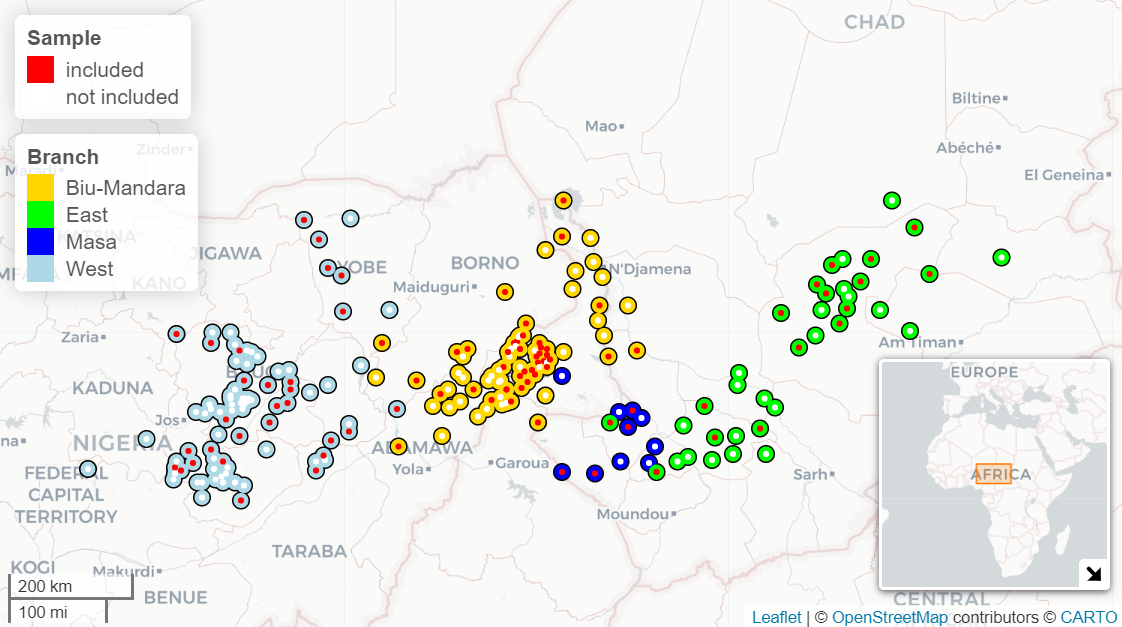
\includegraphics[width=\textwidth]{maps/Chadic.png}
	\caption{Map of Chadic languages based on Glottolog 5.0} \label{map:Chadic}
\end{figure}

The Chadic family is divided into four branches: West, Biu-Mandara, Masa, and East, as illustrated in Figure \ref{fig:Chadic} \citep{newmanComparativeChadicPhonology1966}.\footnote{One severely endangered Biu-Mandara language, Jilbe, has not been assigned to a subbranch of Biu-Mandara.} The geographic distribution of Chadic languages is shown in Figure \ref{map:Chadic}. The 84 West Chadic languages are spoken in the northeastern quadrant of Nigeria. The 80 Biu-Mandara languages (also known as Central Chadic) are spoken in a geographic area spreading across the Far North Region of Cameroon (\textit{Région de l'Extrême-Nord}) and extending westward over the Mandara mountains crossing the Nigerian border and eastward over the Chadian border. There are just ten Masa languages. They are geographically clustered around the southwestern part of Chad near the Cameroonian border. The 36 East Chadic languages are all spoken in the country of Chad.

The main issue of internal classification of Chadic languages has been the status of the Masa languages. \citet{shryockClassificationMasaGroup1997} summarizes the various perspectives on whether the Masa languages should be joined in a single branch with Biu-Mandara, or separated out at the branch level distinct from Biu-Mandara languages. He argues that Masa languages are a separate branch, based on phonological and lexical innovations which only occurred in the (non-Masa) Biu-Mandara languages, concluding that ``there is no conclusive evidence from shared innovations which supports the subclassification of the Masa group of languages in Biu-Mandara'' \citep[45]{shryockClassificationMasaGroup1997}. 

Studies of Chadic languages are mostly of fairly recent production. Only 14\% of the references on Chadic languages listed by Glottolog were published before 1960. There was a peak of publishing activity in the 1990s and early 2000s, as shown in Figure \ref{fig:publications}. This period of increased scholarly work on Chadic languages is all the more remarkable given the recurrent issues of restricted access due to periods of political instability in the region. In the last two decades there has been a decline in the number of publications on Chadic languages. This may be partially explained by a delay in incorporating recent publications into Glottolog's database, but it also coincidences with the retirement of a cohort of prominent Chadicists alongside very little evidence of continued institutional support for the study of African languages.

\begin{figure}
	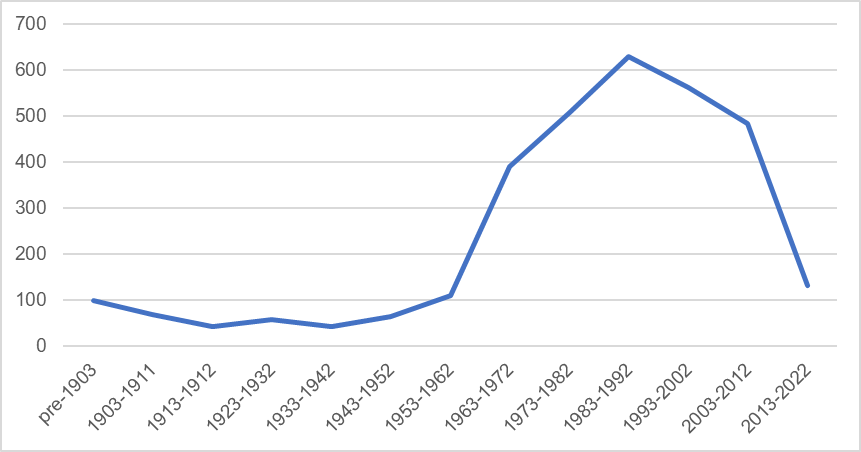
\includegraphics[width=\textwidth]{figures/publications.png}
	\caption{Number of publications on Chadic languages by decade} \label{fig:publications}
\end{figure}

In addition to publishing grammatical description of many Chadic languages, several authors have also published comparative overviews of the language family. Most of these are short summaries based on the author's own impression of general trends in the literature with clear bias toward languages that the author had firsthand experience studying \citep{newmanChadicLanguages2003,schuhChadicOverview2003,frajzyngierChadic2012,jaggarChadicLanguages2006,creisselsAfricaMorphosyntacticArea2008,jungraithmayrChadic2012,wolffChadicLanguages2014,caronChadic2020}.

The most substantial typological publication on Chadic languages is the unfinished work of \citet{schuhChadicCornucopia2017}, published posthumously. Schuh takes a historical-comparative approach, blending synchronic and diachronic analysis, and frequently proposing reconstructed forms based on a small sample of languages. By Schuh’s own admission, his work is somewhat biased toward the West Chadic languages he studied, and he had limited access to descriptions of East Chadic languages. Schuh’s overview of Chadic is illustrated by a small number of selected languages, and does not give a quantitative overview of how grammatical features are distributed among Chadic languages. It therefore remains uncertain how precisely Schuh's observations characterize Chadic languages as a family. 

The analysis of Chadic directional extensions in this book builds on the foundation of previous grammatical descriptions and typological generalizations. It provides a more precise quantitative approach to studying the distribution of grammatical features across Chadic languages. The intent is to align Chadic linguistics with typology in the sense of \citet[6]{bickelTypology21stCentury2007} who characterizes it as ``a discipline that develops variables for capturing cross-linguistic similarities and differences (qualitative typology), explores universal and local skewings in the distribution of these variables (quantitative typology) and proposes theories that explain the skewings (theoretical typology).''

By approaching the topic of motion in the grammar of Chadic languages from the perspective of modern typology, this work also provides a countermeasure to the relative lack of research being done on Chadic languages within Afroasiatic scholarship. Anecdotally, an online search of the contents of \textit{Brill's Journal of Afroasiatic Languages and Linguistics} brings up only four articles on Chadic languages in the 15 years since the inception of the journal in 2009. Using references in the Glottolog bibliography \citep{hammarstromGlottolog502024} as a measure of how thoroughly each language family has been studied, Ancient Egyptian is by far the most well-studied family with 254 references for just two languages. Three families have similar average numbers of references per language: Berber, 42.6; Cushitic, 47.4; Semitic, 39.2. The average number of references per language is much lower for Chadic languages at just 15.2.

Even for linguists with a more narrow focus on another family of Afroasiatic languages, parallel work on Chadic languages can provide crucial insights. As a relevant example of this, \citet[133]{fixSemanticsSemiticVentive2020} reviews over a century of studies of the ventive form of Akkadian verbs, including the work of no less than 30 scholars, concluding that: ``The reality is that despite some advances in terminology and categorization of ventive uses... the discussion of the Akkadian ventive has not actually progressed much from where Landsberger originally brought us with his [1924] article.'' The considerable effort given to the study of a single morphological form in a single extinct language did not prove to be a particularly fruitful approach. \citet[]{fixSemanticsSemiticVentive2020} instead proposes an approach that relies on insights from cross-linguistic studies. This book on directional extensions (including ventive forms) in Chadic languages provides a robust comparative picture of this topic, particularly from an Afroasiatic perspective. 

In addition, it is hoped that this work might kindle interest in the linguistic knowledge and creativity of the speakers of hundreds of understudied Afroasiatic languages spread across Africa. While there has been notable progress in describing and documenting Chadic languages, the reality is that the majority of Chadic languages have only minimal documentation, and many have never been studied. In some cases, their existence has only recently been documented \citep{blenchFiveUnexpectedChadic2016,blenchNewApproachesWest2017}. The opportunity to learn about Chadic languages may only be for a limited period of time, as speakers of the world's minoritized languages are under continual pressure to abandon their heritage languages leading to loss of linguistic knowledge within a few generations \citep{bromhamGlobalPredictorsLanguage2021,campbellNewKnowledgeFindings2013,simonsTwoCenturiesSpreading2019}.

\section{Comparing multi-functional morphemes} \label{sec:comparing}

As is now common practice in comparative linguistics (or typology), the concept of \textit{directional extensions} as applied in this cross-linguistic study is proposed as a \textit{comparative concept}, constructed by a linguist for the purpose of comparing linguistic systems, and not a \textit{cross-linguistic category}, a kind of naturally occurring entity that can be diagnosed as having the same set of properties across languages \citep{haspelmathPreestablishedCategoriesDont2007, haspelmathComparativeConceptsDescriptive2010}. Even very similar morphemes in different languages are not assumed to be identical in their morphosyntactic and semantic properties. For example, identifying morphemes in different languages as meeting the definition of \textit{ventive extensions} (as a comparative concept) does not entail that those morphemes will have the same range of functions, the same morphosyntactic distribution, or the same diachronic development. 

Given that directional extensions have not been central to theories of universal linguistic structures, there are no unnecessary controversies to unravel regarding the status of directionals as a cross-linguistic category. However, a linguist describing a particular language may find that the comparative concepts used in this book do not capture the particularities of that language's verbal morphology in a natural or insightful manner. This is unproblematic because comparative concepts are distinct from language-particular categories. 

For example, the West Chadic language \hyperref[kana]{Kanakuru} has two morphemes which meet the definition of the comparative concept \textit{ventive direction extension} described in Chapter \ref{ch:identifying}. One is a verbal suffix \textit{-tə(ru)} and the other is a preverbal particle \textit{bo}. Naturally, \citet{newmanKanakuruLanguage1974} distinguishes these forms, describing one as a ``ventive suffix'' and the other as a ``ventive equivalent auxiliary''. From a cross-linguistic perspective, it is noteworthy that this is the only example of a pre-verbal directional extension in the data. At the same time, it would not be worth refining the comparative concept to distinguish pre-verbal and post-verbal extensions for one outlier in the data. Therefore, the two distinct morphemes in Kanakuru are both treated as ventive extensions in regard to cross-linguistic generalizations.

While \textit{directional extension} as a comparative concept is narrowly defined without regard to the full semantic profile of each morpheme, the multi-functionality of directional extensions is not being ignored. Rather, a fundamental contribution of this research project is to provide a quantitative analysis of multi-functional morphemes. Once a set of verbal extensions with directional semantics is identified, it is then possible to ask what other functions these same forms have. The term ``co-expression'' is used to described ``the relation between a linguistic form in a given language and several functions that are expressed by different forms in some other language'' \citep[476]{hartmannIdentifyingSemanticRole2016}. 

For example, in \hyperref[huba]{Huba}, the same verbal extension that expresses downward direction in one context (in \ref{ex:huba3b} above) can express completive aspect in another context, as in (\ref{ex:huba02b}). In contrast, in most languages, aspectual meanings like completive are expressed by forms distinct from morphemes that express downward direction. Therefore, this one form in Huba is considered to co-express (at least) two functions. Nonetheless, the suffix \textit{-yà} is considered a directional extension because it has a directional function in (\ref{ex:huba3b}), irrespective of what functions it may co-express.

\ea\label{ex:huba02b}
\langinfo{\hyperref[huba]{Huba} verb \textit{wùr} `finish' with downward suffix}{}{\cite[108]{muazuGrammarKilbaLanguage2009}} \\
\gll wùr-yà	\\
finish-\gl{down}	\\
\glt `to finish completely'
\z 

\section{Motion in grammar} \label{sec:motion}

The universality, salience and complexity of motion in grammar has held the attention of linguists for decades. Motion entails a conceptualization of both space and time. Much of the work on motion in language has had an aim of gaining insights into human cognition by comparing how people from different cultures and languages might think differently about space and time. For example, well-known work of \citet{levinsonSpaceLanguageCognition2003} and \citet{levinsonGrammarsSpaceExplorations2006} highlights the diverse frames of reference (intrinsic, relative, absolute) applied to descriptions of location and motion, as well as the the diversity of how frame of reference is encoded in linguistic structures. They discuss how speakers of languages with grammaticalized forms for expressing cardinal directions are consistently able to identify cardinal directions and to recall the cardinal orientation of past events. Other researchers have focused on the morphosyntactic representation of the source and goal of motion events in adpositions and case marking or in adverbial interrogatives and demonstratives \citep{creisselsEncodingDistinctionLocation2006, kopeckaSourcegoalAsymmetriesLanguages2021, nintemannHereHitherHence2020, stolzCrosslinguisticsZeromarkingSpatial2014, stolzSpatialInterrogativesEurope2017}.

Much of the terminology commonly found in descriptive and comparative studies of motion events is drawn from the work of \citet{talmyLexicalizationPatternsSemantic1985}  \citep[see also][25--26]{talmyCognitiveSemantics2000}. Motion events exclude self-contained (or non-translational) motion, as in \textit{The log rolled over and over in water}, but include stationary (or stative) location. In a motion event, a person or object (the figure) is described as maintaining or changing location relative to some other entity (the ground). If the location changes (translational motion), the characterization of how the position of the figure changes with respect to the ground is known as the path of motion. 

Generally, linguistic expressions describing a change of location do not include a precise, detailed retracing of the geometry of the path of motion, but will rather reference a few relevant aspects of the path of motion. The description of the path might only give a single point of reference, for example, away from a source or towards a goal. The source or goal of the path may be identified with the notion of a deictic center: a fixed point of reference typically corresponding to the location of the speaker, as in `here'. More complex geometric notions can also be included in the description of the path of motion. For example, a boundary-crossing path is defined in reference to a bounded space (e.g., \textit{into a house} or \textit{out of a box}).%\footnote{\citet[53]{talmyCognitiveSemantics2000} refers to these components of describing a path of motion as ``Vector'', ``Deictic'' and ``Conformation''.}

Semantic content defining the path of motion can be included in the meaning of a motion verb. For example, the motion interpretation of the English verb \textit{enter} in the phrase \textit{They entered the house} entails that a figure (referenced by the subject) moves along a path of motion which begins outside of a bounded space (`the house') and crosses the boundary to an endpoint within the bounded space. It is also common for a verb of motion to be modified by some other morpheme which adds details about the path of motion. For example, the English preposition \textit{into} has a meaning similar to the verb \textit{enter}. The preposition can be combined with a generic motion verb as in \textit{move into the circle} to express an inward path of motion without the direction being defined by the verb itself.

\citet{talmyPathRealizationTypology1991} created a dichotomous typology by distinguishing cases where information about the path of motion is expressed by the main verb of a clause from all other possible ways of expressing a path of motion. In this approach, linguistic expressions of motion events are either ``verb-framed'' (the path is expressed by the main verb) or ``satellite-framed'' (the path is expressed elsewhere).\footnote{Talmy's original typology focused on categorizing language types. However, most languages allow for more than one way to express the path of motion, and so a typology of language types relies on an assessment of speakers' or signers' general tendencies when using the language. This rather vaguely defined notion was later made more precise by researchers who applied these concepts to describing types of linguistic expressions or grammatical constructions rather than types of languages \citep[e.g.][]{beaversTypologyMotionExpressions2010,croftRevisingTalmyTypological2010}.} Under Talmy's approach, ``satellites'' would include verbal morphology, adverbial expressions and subordinate verbs \citep[103]{talmyCognitiveSemantics2000}.\footnote{Talmy argues that even in the case of serial verb constructions where the syntactic relationship between the verbs in a clause does not have the grammatical properties typically associated with subordination it should, in principle, be possible to identify one of the verbs in the construction as the main verb and the other as a satellite \citep{talmyPropertiesMainVerbs2016}.}

Chapter \ref{ch:verbs} takes an alternate perspective on Talmy's typology of the expression of the directional meaning. Rather than examining speakers' preferences for choosing between forms which express directional meaning in the verb (verb-framed) or elsewhere (satellite-framed), this chapter looks at the availability of expressing direction either in the root of a motion verb or as a verbal extension. For certain types of direction, there is a pattern of complementary distribution within the verbal complex such that the direction is either lexicalized in the verb root or grammaticalized in the verbal morphology, but not both. This can be viewed as a type of efficiency in the grammar, avoiding redundant expression of the same meaning in multiple forms. However, for ventive and itive directional meaning, redundancy is more common than complementary distribution. 

While the research presented in this book relies on Talmy's conceptual and terminological work, it is not a Talmian typological analysis of the expression of motion in verbs and satellites. The starting point is not how the elements of motion are expressed across syntactic constructions, but rather the expression of path of motion in the verbal extensions. This set of morphemes is narrower than the broad concept of satellites. It does not include adverbs, subordinate verbs or serial verb constructions. Semantically, the primary interest in this work is the limited number of directional meanings that are frequently expressed in verbal extensions in Chadic languages.\footnote{The expression of these directional meanings in verb roots is discussed in Chapter \ref{ch:verbs}.}
 
Directional semantics have been included as an element of many previous typological studies; however, there has not been a particular focus on directional verbal morphology until recently. It was in the process of studying associated motion\index{associated motion} morphology that several authors noted the need to distinguish directional morphemes from associated motion, leading to the topic of directional morphology receiving more attention in its own right \citep{bourdinMarkingDirectionalDeixis2006,belkadiAssociatedMotionDeictic2015,guillaumeAssociatedMotionSouth2016}. It is in the context of discussing associated motion that \citet{rossCrosslinguisticSurveyAssociated2021,rossPseudocoordinationSerialVerb2021} provides a global cross-linguistic quantitative study of directional verbal morphology. Part of the research presented in this book contains a study similar to \citet{rossCrosslinguisticSurveyAssociated2021} but focused on Chadic languages (Chapters \ref{ch:identifying}, \ref{ch:identifying2} and \ref{ch:distribution}).

One of the particular areas of interest in the typology of directional verbal morphology has been the co-expression of associated motion\index{associated motion} with directionality \citep{dryerAssociatedMotionDirectionals2021,belkadiDeicticDirectionalityAssociated2021}. An example of this can be seen in \hyperref[zulg]{Zulgo-Gemzek} where the verbal extension \textit{-áha} can have a directional function (itive) with a motion verb, as in (\ref{ex:zulg4}), but can also have a subsequent associated motion meaning with a non-motion verb, as in (\ref{ex:zulg6b}). The crucial distinction is that in (\ref{ex:zulg6b}), the meaning of the verb does not entail any motion -- the motion event is due to the presence of the verbal extension. 

\ea\label{ex:zulg4}
\langinfo{\hyperref[zulg]{Zulgo} verb \textit{val} `run' with itive suffix}{}{\cite[47]{hallerVerbalComplexZulgo1981}} \\
\gll á-val-áha \\
he-ran-\gl{itive} \\
\glt `He ran there.'

\ex\label{ex:zulg6b}
\langinfo{\hyperref[zulg]{Zulgo} verb \textit{zə́m} `eat' with itive suffix}{}{\cite[47]{hallerVerbalComplexZulgo1981}} \\
\gll á-zə́m-áha daf \\
he-ate-\gl{itive} fufu \\
\glt `He ate fufu and went there.'
\z 

This issue is explored for Chadic languages in Chapters \ref{ch:functions} and \ref{ch:interpretation}. The database created for this research (Chapter \ref{ch:identifying2}, Section \ref{sec:database}) tracks what meanings are co-expressed with directional meaning, including associated motion\index{associated motion}, allowing a quantitative approach to studying the multi-functionality of motion morphology (Chapter \ref{ch:functions}) including which meanings occur with what verb roots (Chapter \ref{ch:interpretation}).

Another domain of motion research in linguistics that has recently been given more attention is the expression of bringing and taking events, which \citet{margettsCausedAccompaniedMotion2022} call \textit{directed caused accompanied motion} (directed CAM). Chapter \ref{ch:CAM} contributes to this relatively new area of focus by presenting a distributional typology of directed CAM in Chadic languages. 

Finally, this book contributes to the empirical study of motion in language by improving the state of art in the description of Chadic languages. The appendices present a brief description of the directional verbal morphology and other related aspects of 91 Chadic languages. A major aim of this book is to provide a tool that helps linguists have more appropriate concepts and vocabulary for understanding and describing the expression of motion in the grammars Chadic languages, thus contributing to the ``persistent need to document expressions of spatial relations and motion events in natural languages'' \citep[14]{robbersOrientationMotionWorld2023}. 

\section{Overview of this book} \label{sec:overview}

The remainder of this book is divided into seven core chapters followed by a brief summary chapter. Chapter \ref{ch:identifying} defines and exemplifies the semantic subtypes of directional extensions found across Chadic languages. Chapter \ref{ch:identifying2} is closely related in that it provides further clarification on how particular linguistic examples were classified, dealing with many-to-one and one-to-many form-function relationships as well as some borderline cases of motion events. This chapter also discusses the implications of these analytical choices for the database used in the quantitative analyses throughout this book.

Chapter \ref{ch:distribution} presents the results of the first quantitative study: how frequently each type of directional extension is found across the 91 Chadic languages included in this research. The most common type is ventive meaning, but among the Biu-Mandara languages many other types of directional meaning are found expressed in verbal extensions. The final section looks at what types of directional extensions co-occur in each language. Although ventive is the most common type, there is no (synchronic) implicational hierarchy that predicts the existence of a ventive directional extension in languages with more than two directional extensions. 

Chapter \ref{ch:diachrony} covers the diachrony of directional extensions in Chadic languages. Naturally, the synchronic comparative data raises questions about the history of these forms that led to their current distribution across Chadic languages. While no particular directional extensions can be reconstructed to a Proto-Chadic form, there are some general patterns that allow some basic hypotheses to be formed. Ventive directional extensions can be plausibly reconstructed for West Chadic languages, but it is uncertain that these forms share a historical relationship with ventive directional extensions in other branches. Most other types of directional extensions have only developed in Biu-Mandara languages and their forms suggest multiple innovations from various sources in different languages.

Chapter \ref{ch:verbs} examines patterns of efficiency and redundancy in grammatical systems by comparing the distribution of directional meaning in verbal extensions with the distribution of the same meaning in verb stems (i.e., directional verbs) in Chadic languages. The results show that vertical (upward, downward) and boundary-crossing (inward, outward) directional meanings have a strong tendency to occur in complementary distribution. Languages with vertical or boundary-crossing directional extensions rarely have these same meanings expressed by vertical or boundary-crossing directional verbs, and vice versa. The same is not true of ventive and itive extensions. These meanings are often redundantly expressed in both a verbal extension and in a verb stem. However, there is a correlation between the presence of a ventive directional extension and having a general motion verb (unspecified for direction). 

Chapter \ref{ch:functions} is an analysis of the non-directional functions co-expressed by directional extensions, including how frequently various functions are co-expressed with each type of directional meaning across the 91 languages in the sample. The most commonly reported meanings co-expressed with directional meaning in verbal extensions are other types of motion or location meaning, especially subsequent associated motion\index{associated motion}. In addition to these functions, a directional extension may lexicalize in combination with a particular verb to express an idiomatic or non-compositional predicate meaning, much like phrasal verbs in English. It is also commonly reported that directional extensions co-express an aspectual meaning or have other grammaticalized, non-motion functions; however, such claims are often made without the support of clear contrastive evidence from language data.  

Chapter \ref{ch:interpretation} expands on the study of co-expression of various meanings in verbal extensions to examine whether the lexical semantics of the verb stem is predictive of the interpretation of the verbal extension. As expected, a verbal extension that can express directional meaning nearly always does so when modifiying a motion verb, but this is not without exceptions. A number of verbs, such as verbs of hitting or removing, are not typical motion verbs but can be construed as happening along a path of motion when combined with a directional extension. However, verbal extensions combined with the same verbs are also frequently given other motion-related interpretations (such as subsequent or resultative motion). Overall, the conclusion is that the lexical semantics of the verb may correlate with a particular interpretation of a directional extension, but the meaning of the verb on its own does not fully determine how the verbal extension will be interpreted. 

Chapter \ref{ch:CAM} is the first of two chapters that take a broader perspective on directional extensions in Chadic languages by selecting a particular semantic domain (or function) in which directional extensions are frequently found, and then comparing how that semantic domain is linguistically structured across Chadic languages. The first domain examined is directed caused accompanied motion (CAM), as in the English verb `bring'. One of the two most frequent ways of expressing directed CAM is to combine a verb of possession, e.g., `take', with a directional extension. It is slightly more common to find directed CAM expressed by a directional verb with valency-increasing morphology. It is argued that both of these forms are lexicalized or idiomatic expressions of directed CAM, contrary to previous approaches that assume they can be synchronically parsed (i.e., semantically decomposed) maintaining a standard directional or causative interpretation of the verbal morphology. 

\largerpage
Chapter \ref{ch:buysell} presents a second semantic domain in which directional extensions are commonly found in Chadic languages: the distinction between the notions `buy' and `sell'. These notions differ only in regard to whether the primary argument is the one giving or receiving money in the transaction -- a distinction that would only have become relevant millenia after the Chadic languages began to spread across the Sahel region. In order to make this distinction, many Chadic languages have borrowed a verb for `sell' or extended the meaning of another verb to express `sell'. It is also common to find languages with a verb that can be translated as either `buy' or `sell' but which can take additional verbal morphology to make the distinction explicit. This morphology is typically either a directional extension or a valency-increasing morpheme. Which form is used (including which directional path is used in the case of directional extensions) is not predictable from language to language. This indicates that these are lexicalized verb-extension combinations created to fill the functional need that arose with the introduction of currency. 

\largerpage
Chapter \ref{ch:summary} is a brief summary. This is followed by an extended appendix which presents the analysis of the relevant data for each of the 91 languages included in this study. Throughout this book, the names of languages in the sample are hyperlinked to the section in the appendix that gives an overview of the data for that language.

 
\chapter{Defining directional extensions} \label{ch:identifying}

This chapter defines and exemplifies the types of directional extensions found in Chadic languages. Section \ref{sec:path} further defines the morphosyntactic notion \textit{verbal extension} and the semantic concept \textit{direction}. The remaining sections each describe and exemplify a particular sub-type of directional extension found in Chadic languages: ventive (Section \ref{sec:vent1}), itive (Section \ref{sec:itive1}), inward and outward (Section \ref{sec:bounded1}), upward and downward (Section \ref{sec:vertical1}), `onto' and `under' (Section \ref{sec:onto1}). A few marginal types are presented in Section \ref{sec:otherDIR1}: homeward, bushward and `side'. The results of a quantitative study looking at how common each subtype of directional extensions is across the branches of Chadic languages is presented in Chapter \ref{ch:distribution}. Before that chapter, Chapter \ref{ch:identifying2} further explains how types of directional extensions were identified in published sources and organized into a database for quantitative analysis. 

\section{Directional extensions} \label{sec:path}

In the analysis of Chadic languages, verbal morphology is typically organized into three categories. First, there is normally verbal morphology expressing notions related to tense-aspect. Second, there is often a type of verbal morphology that has argument agreement or pronominal functions. Third, verbal morphology not falling into one of those two categories are frequently described as \textit{verbal extensions}.

Verbal extensions may be affixes or particles (morphologically detached from the verb) but all extensions are morphosyntactically dependent on the verb. Non-concatenative verbal morphology and irregular verbal conjugations are also considered types of verbal extensions. Unlike adverbs, a verbal extension cannot modify a nonverbal predicate or be used independently of a verb. Even if the verb may be elided (e.g., in response to a question) a verbal extension cannot be uttered on its own without a verb. Verbal extensions have fixed positions in the verbal phrase (typically following the verb), and do not exhibit variable syntactic positioning such as being able to appear at the beginning of a clause. In principle, the distinction between verbal extensions and other categories is not fuzzy, but it is not always clear how to diagnose a particular morpheme from the available documentation and description.

Practically speaking, available descriptions are generally taken at face value, and any directional morpheme described as a part of the verbal morphology is usually considered an extension. However, there are a few disputable descriptions. In \hyperref[tera]{Tera}, \citet[18]{newmanGrammarTeraTransformational1970} describes the form \textit{ɓara} as a ``particle'' but \citet[314--315]{schuhChadicCornucopia2017} points out that it has the syntactic distribution of an adverb. Some \hyperref[masa]{Masana} morphemes are described as verbal extensions, but also have uses in nonverbal clauses which (at least in this book) places them in the category of adverbs \citep[226]{melisDescriptionMasaTchad1999}. In a description of \hyperref[bura]{Bura}, \citet[284--289]{hoffmannUntersuchungenZurStruktur1955} describes several forms as phonetic contractions of a verb and an adposition or noun, rather than as productive verbal morphology. These few examples are not considered verbal extensions in this work.

One common function of verbal extensions in Chadic languages is to add directional information about a path of motion.\footnote{In addition to directional extensions, another common function of verbal extensions in Chadic languages is to modify the argument structure or valency of the verb.} Directional extensions are verbal extensions that can (as at least one of their uses) be added to a verb expressing a (translocative) motion event in order to specify the orientation of the path of motion. Directionals are frequently shown to combine with intransitive verbs of motion, for example, a manner-of-motion verb, as in (\ref{ex:muse1}), or a directional verb, as in (\ref{ex:bura6}). Note that in (\ref{ex:bura6}), information about the direction of the path of motion comes from both the ventive directional verb as well as the downward directional extension.  

\ea\label{ex:muse1}
\langinfo{\hyperref[muse]{Musey} verb \textit{līŋ} `run' with ventive marker}{}{\cite[76]{dassidiMorphophonologicalStructureMusej2015}} \\
\gll Sánàmā līŋ-áj tá ànú	\\
Sanama run-\gl{vent} body \gl{1}\gl{sg}.\gl{obj} \\
\glt `Sanama ran towards me.'

\ex\label{ex:bura6}
\langinfo{\hyperref[bura]{Bura} verb \textit{si} ‘come’ with the downward suffix}{}{\cite[281]{hoffmannUntersuchungenZurStruktur1955}} \\
\gll si-hi \\
come-\gl{down} \\
\glt `come down' [German: `\textit{herunterkommen}']
\z 

Semantically there are eight predominant types of directional meaning expressed in verbal extensions in Chadic languages. These can be seen as four pairs of semantic counterparts: ventive-itive, inward-outward, upward-downward and onto-under. Ventive and itive direction are defined in relation to a deictic center. Ventive is movement toward a deictic center (deictic center is the goal) (Section \ref{sec:vent1}), and itive is motion away from a deictic center (Section \ref{sec:itive1}).\footnote{Note that itive motion is only the antonym of ventive motion if the source of the itive path of motion is the deictic center. See Section \ref{sec:itive1} for discussion of the itive directional extension in \hyperref[buwa]{Buwal} which has a source of motion other than the location of the speaker.} The deictic center is a relative notion, like the adverbial `here'. An understanding of where the deictic center is understood to be can only be derived from context. 

Upward and downward motion are defined in relationship to vertical space, with the earth's surface (or the direction of gravity) as the point of reference (Section \ref{sec:vertical1}). Inward and outward direction are defined in relation to a bounded or enclosed space (as in `enter' and `exit') (Section \ref{sec:bounded1}). Directional extensions meaning `onto' describe a path of motion which moves toward the uppermost surface of some object (Section \ref{sec:onto1}). The counterpart is a more rare `under' directional extension that describes a path of motion ending at or passing through a point below some object. There are also a few even rarer types of directional extensions discussed in Section \ref{sec:otherDIR1}.

\section{Ventive directional extensions} \label{sec:vent1}

A ventive directional extension combined with a motion verb has the function of indicating that the path of motion is directed toward the deictic center. In many contexts, the deictic center will be understood to be the location of the speaker, but this will not always be the case. Precisely how the deictic center is pragmatically interpreted will not be explored here. It will simply be inferred from available translations whether a particular form expresses movement toward or away from a deictic center.\footnote{Assuming that translations consistently reflect the deictic orientation is not without complications. In the descriptions of four languages, there is at least one example of a ventive extension that is given an exceptional itive translation (\hyperref[mina]{Mina}, \hyperref[mbuk]{Mbuku}, \hyperref[mbud]{Mbudum}, \hyperref[mada]{Mada}), and in two examples an itive extension is given a ventive translation (\hyperref[zulg]{Gemzek} and \hyperref[gaan]{Ga'anda}). These exceptions are left aside without explanation.} 

Several different labels are used for ventive directional extensions in descriptions of Chadic languages, including \textit{centripetal} and, in French, \textit{rapprochement}. They are sometimes simply called \textit{directional}. A ventive extension may be found with a manner-of-motion verb to indicate in which direction the motion occurs, as in (\ref{ex:vame1}) and (\ref{ex:mofu1}).

\ea\label{ex:vame1}
\langinfo{\hyperref[vame]{Vamé} verb \textit{hav} `fly' with ventive suffix}{}{\cite[56]{kinnairdVameVerbalSystem2006}} \\
\gll  fan hav-ki-ke	\\
bird fly-\gl{vent}-\gl{prf}	\\
\glt `The bird is flying (towards us).'

\ex\label{ex:mofu1}
\langinfo{\hyperref[mofu]{Mofu} verb \textit{há} `run' with ventive suffix}{}{\cite[70]{barreteauDescriptionMofuGudurLangue1983}} \\
\gll há-wa \\
run-\gl{vent} \\
\glt `Come here quickly!' [French: `\textit{Viens-vite ici} !']
\z 

A ventive extension can also combine with a directional motion verb that indicates a different parameter of direction, such as the downward motion verb in (\ref{ex:tang1}) which combines with a ventive extension indicating that the motion is both downward and toward the deictic center (the inverse pattern of \ref{ex:bura6}). 

\ea\label{ex:tang1}
\langinfo{\hyperref[tang]{Tangale} verb \textit{yẹk} `descend' with ventive suffix}{}{\cite[47]{jungraithmayrDictionaryTangaleLanguage1991}} \\
\gll n yẹk-tụ́-ngọ	\\
\gl{1}\gl{sg} descend-\gl{vent}-\gl{1}\gl{sg}	\\
\glt `I came down.'	
\z

In several languages, there is a general motion verb which does not entail any specific direction of its path (Chapter \ref{ch:verbs}, Section \ref{sec:motionV}). In a neutral context, the implied path might be itive (away from the deictic center) or ventive. In the two instances of the \hyperref[buwa]{Buwal} verb \textit{nda} in (\ref{ex:buwa1}) each token has a different interpretation (in the original text, one is glossed `come' and one is glossed `go'). The same verb can combine with a ventive extension to explicitly express ventive motion, as in (\ref{ex:buwa100}). 

\ea\label{ex:buwa1}
\langinfo{\hyperref[buwa]{Buwal} verb \textit{nda} meaning `come' and `go' }{}{\cite[365]{viljoenGrammaticalDescriptionBuwal2013}} \\
\gll  màdā māwàl ká-\textbf{ndā} āzá nèné-ná-\textbf{ndā} á eɡljz \\
if husband \gl{pfv}-go/come \gl{compl} \gl{1}\gl{excl}.\gl{sbj}-\gl{fut}-go/come \gl{prep} church \\
\glt `If my husband has come, we will go to church.'

\ex\label{ex:buwa100}
\langinfo{\hyperref[buwa]{Buwal} verb \textit{nda} `go/come' with ventive extension}{}{\cite[373]{viljoenGrammaticalDescriptionBuwal2013}} \\
\gll ná-\textbf{ndā}-xā ná-ndzā á bwāl \\
\gl{1}\gl{excl}.\gl{sbj}-go/come-\gl{vent} \gl{sbj}.\gl{1}\gl{pl}.\gl{excl}-stay \gl{prep} Buwal	\\
\glt `...we came, we stayed in Buwal village. (Speaker is located in Buwal village.)'
\z

Ventive extensions can also be used with transitive (caused) motion verbs where the object is a figure on a path of motion. In (\ref{ex:shaa2}), the translation describes an event in which both the subject and object are moving along a path of motion toward the deictic center.

\ea\label{ex:shaa2}
\langinfo{\hyperref[shaa]{Ron-Scha} verb \textit{də̀ŋ} `pull' with ventive suffix}{}{\cite[268]{jungraithmayrRonSprachenTaschadohamitischeStudien1970}} \\
\gll də̀ŋ-ó \\
pull-\gl{vent} \\
\glt `drag here' [German: `\textit{her-ziehen}']
\z 

\section{Itive directional extensions} \label{sec:itive1}

Itive direction is the counterpart of ventive, describing a path of motion that leads to a location farther from the deictic center. For example, in (\ref{ex:buwa10}), the \hyperref[buwa]{Buwal} itive extension \textit{āzà} combines with a manner-of-motion verb to express that the figure on the path of motion moves away. 

\ea\label{ex:buwa10}
\langinfo{\hyperref[buwa]{Buwal} verb \textit{xēj} `run' with itive extension}{}{\cite[280]{viljoenGrammaticalDescriptionBuwal2013}} \\
\gll ā-xēj āntā āzà skʷá	\\
\gl{3}\gl{sg}.\gl{sbj}-ran \gl{3}\gl{sg}.\gl{poss} \gl{itive} \gl{q}	\\
\glt `…did he run away?'	
\z

Itive directionals are generally presented as antonyms of ventive directionals, but this is not always the case. In \hyperref[buwa]{Buwal}, the ventive and itive directional extensions can co-occur, as in (\ref{ex:buwa01}). This is possible because they do not have the same deictic reference point.

\ea\label{ex:buwa01}
\langinfo{\hyperref[buwa]{Buwal} verb \textit{tàdàkʷ} `descend' with ventive and itive directionals}{}{\cite[378]{viljoenGrammaticalDescriptionBuwal2013}} \\
\gll xʷné-tàdàkʷ-xā āzà á tā xājāk \\
2\gl{pl}.\gl{sbj}-descend-\gl{vent} \gl{itive} \gl{prep} on ground\\ 
\glt `You come down from there onto the ground! (Speaker on the ground.)'
\z

According to \citet[378]{viljoenGrammaticalDescriptionBuwal2013}, the source of the `away' itive motion cannot be the speaker. In (\ref{ex:buwa01}), the source location is up in a tree while the speaker is on the ground. The goal of the ventive motion is the speaker, who is on the ground. The combination of ventive and itive can be analyzed as `move towards me (on the ground) [ventive] and away from that tree [itive]'. Other descriptions of Chadic languages do not necessarily contain this level of detail about the source of an itive path of motion. For this study, all directional extensions described as expressing that a path of motion is `away' are grouped together as itive irrespective of how the source of that path is defined.

As mentioned, some Chadic languages have a general motion verb without any inherent directional meaning, such as \textit{d} in \hyperref[cuvo]{Cuvok} which can be combined either with a ventive extension, as in (\ref{ex:cuvo1}), or an itive extension, as in (\ref{ex:cuvo2}).

\ea\label{ex:cuvo1}
\langinfo{\hyperref[cuvo]{Cuvok} verb \textit{d} `go/come' with ventive suffix}{}{\cite[303]{dadakGrammaireCuvokLangue2021}} \\
\gll d-ɛ́k	\\
go/come-\gl{vent} \\
\glt `Come here.'

\ex\label{ex:cuvo2}
\langinfo{\hyperref[cuvo]{Cuvok} verb \textit{d} `go/come' with itive suffix}{}{\cite[308]{dadakGrammaireCuvokLangue2021}} \\
\gll d-áɗ \\
go/come-\gl{itive} \\
\glt `Go over there.'
\z 

Itive extensions are also found with transitive motion verbs in which the patient is the figure on a path of motion away from the deictic center, as in (\ref{ex:marg3}). 

\ea\label{ex:marg3}
\langinfo{\hyperref[marg]{Margi} verb \textit{ndàl} `throw' with itive suffix}{}{\cite[131]{hoffmannGrammarMargiLanguage1963}} \\
\gll ndàl-nà	\\
throw-\gl{itive}		\\
\glt `to throw away'
\z 

\section{Boundary-crossing directional extensions} \label{sec:bounded1}

Boundary-crossing directional extensions express one of a pair of directional meanings: inward or outward. Inward and outward directional extensions can be combined with directional motion verbs, such as the ventive and itive verbs in (\ref{ex:psik12}) and (\ref{ex:saku5}). They can also be combined with manner-of-motion verbs, as in (\ref{ex:marg6b}).

\ea\label{ex:psik12}
\langinfo{\hyperref[psik]{Psikye} verb \textit{dze} `go' with inward suffix}{}{\cite[118]{smithKapsikiLanguage1969}} \\
\gll pa dze-mbé cɛ	\\
then go-\gl{into} house	\\
\glt `Then (he) went into the house...'

\ex\label{ex:saku5}
\langinfo{\hyperref[saku]{Sakun} verb \textit{ja} `come' with outward suffix}{}{\cite[126]{thomasGrammarSakunSukur2014}} \\
\gll má ja-vá-j ja-vá kwá ná … \\
when come-\gl{out}-\gl{prog} come-\gl{out} \gl{2}\gl{sg} \gl{top} \\
\glt `Immediately when you come out...'

\ex\label{ex:marg6b}
\langinfo{\hyperref[marg]{Margi} verb \textit{mə̀} `run' with outward suffix}{}{\cite[122]{hoffmannGrammarMargiLanguage1963}} \\
\gll mə̀-bá	\\
run-\gl{out}		\\
\glt `to start up and run out'
\z

Inward and outward extensions are also found with transitive motion events, as in (\ref{ex:marg12}) and (\ref{ex:bura16}).

\ea\label{ex:marg12}
\langinfo{\hyperref[marg]{Margi} verb \textit{f} `put' with inward suffix}{}{\cite[148]{hoffmannGrammarMargiLanguage1963}} \\
\gll  f-wá	\\
put-\gl{into} \\
\glt `to put (one) into'

\ex\label{ex:bura16}
\langinfo{\hyperref[bura]{Bura} verb \textit{buka} ‘push’ with outward suffix}{}{\cite[4]{blenchBuraVerbalExtensions2010}} \\
\gll  buka-ɓəla \\
push-\gl{out} \\
\glt `to push outside'
\z  

Inward and outward directional meanings are defined in relation to any space perceived as having an enclosed boundary. This can be as concretely defined as a jar or a house, as in (\ref{ex:psik12}), or it can be more abstractly defined, for example, as a fire which has no fixed borders, as in (\ref{ex:dghw800}).

\ea\label{ex:dghw800}
\langinfo{\hyperref[dghw]{Dghwede} verb \textit{ə̀yə̂} `fall' with inward suffix}{}{\cite[25]{frickVerbalSystemDghwede1978}} \\
\gll ə̀yə̂-me cé ne dá me kárà... \\
fall-\gl{into} \gl{past} ?? to ?? fire \\
\glt `when he had fallen into the fire'
\z 

In \hyperref[mata]{Matal}, there are two inward directional extensions which are semantically distinguished by whether the bounded area is enclosed (e.g., with a cover) or not. The form \textit{ába} is used for uncovered containers, such as the pipe in (\ref{ex:mata10}), and \textit{águ} is used for covered containers, as in (\ref{ex:mata11}) \citep[76]{dougopheGrammarMatal2021}.\footnote{Note that further data is needed to more definitively determine the morphosyntactic status of these morphemes---whether they are part of the verbal system or adverbials.}

\ea\label{ex:mata10}
\langinfo{\hyperref[mata]{Matal} verb \textit{d} `go' with inward extension}{}{\cite[180]{dougopheGrammarMatal2021}} \\
\gll áŋá ákàl à-dá-d ábà jkə̀nj á-s-àl=àw	\\
if fire \gl{3}\gl{sg}-\gl{pfv}-go inside too \gl{3}\gl{sg}-please-\gl{3}\gl{sg}.\gl{dat}=\gl{neg}	\\
\glt `If heat enters the pipe, it does not like/it is not good.'

\ex\label{ex:mata11}
\langinfo{\hyperref[mata]{Matal} verb \textit{sàkw} `put' with inward extension}{}{\cite[202]{dougopheGrammarMatal2021}} \\
\gll  wànáj xə̀ŋ ka mə̀-sàkw-àx-àj ka kwàndúrkú águ	\\
\gl{dem} (\gl{prox}) \gl{top} \gl{1}\gl{sg}-put-\gl{pl}-?? \gl{top} dolo inside		\\
\glt `As for this one, we put dolo (an unfermented sorghum beverage) inside.'
\z 

\section{Vertical directional extensions} \label{sec:vertical1}

Vertical directional extensions express upward or downward direction. Upward direction can be thought of as a path of motion that moves counter to the direction of gravity, and downward direction is a path of motion in which the figure moves in the same direction as gravity. Upward and downward extensions can combine with directional motion verbs, as in (\ref{ex:malg1}) and (\ref{ex:lama8}), and also with manner-of-motion verbs, as in (\ref{ex:lama15}). 

\ea\label{ex:malg1}
\langinfo{\hyperref[malg]{Malgwa} verb \textit{d} `go' with upward suffix }{}{\cite[153]{lohrSpracheMalgwaNara2002}} \\
\gll də́-tə́ \\
go-\gl{up} \\
\glt `to climb (e.g., up a tree)'

\ex\label{ex:lama8}
\langinfo{\hyperref[lama]{Lamang} verb \textit{s} ‘come’ with downward suffix}{}{\cite[144]{wolffLamangLanguageDictionary2015}} \\
\gll sa-gáa-tá	\\
come-\gl{down}-\gl{compl}	 \\
\glt `coming down'

\ex\label{ex:lama15}
\langinfo{\hyperref[lama]{Lamang} verb \textit{ndr} ‘fly’ with downward suffix}{}{\cite[283]{wolffLamangLanguageDictionary2015}} \\
\gll ɗíyák ndə̀rà-gáa-tá skwè-ɗè	\\
bird fly-\gl{down}-\gl{compl} come-\gl{down}		\\
\glt `The bird flew down.'
\z 

Like other directional extensions, vertical directional extensions are also used with transitive motion verbs, as in (\ref{ex:bura17}). 

\ea\label{ex:bura17}
\langinfo{\hyperref[bura]{Bura} verb \textit{ndzi} ‘throw’ with downward suffix}{}{\cite[281]{hoffmannUntersuchungenZurStruktur1955}} \\
\gll ndzi-hi \\
throw-\gl{down} \\
\glt `throw down' [German: `\textit{niederwerfen}'] 
\z 

\citet[141]{wolffLamangLanguageDictionary2015} describes the \hyperref[lama]{Lamang} upward extension \textit{-fi} as also expressing ``direction east'' and the downward extension \textit{-ɗi} as also expressing ``direction west''. This corresponds to Lamang speakers residing in plains to the west of the northernmost tip of the Mandara mountain range in eastern Nigeria. From this vantage point, moving upwards into the mountains is also moving eastward. Conversely, in \hyperref[glav]{Glavda}, \citet[662]{bubaGlavdaMorphology2007} describe the upward extension \textit{-dit} as having an additional meaning of ``westward'', as in (\ref{ex:glav7}). This corresponds to Glavda speakers residing in an area to the east of the same mountains, and so from their perspective movement into the mountains is movement westward.\footnote{However, \citet{nghagyiyaSketchGlavdaGrammar2011} contradicts \citet[662]{bubaGlavdaMorphology2007} and instead associates the upward extension with `eastward'.} 

\ea\label{ex:glav7}
\langinfo{\hyperref[glav]{Glavda} verb \textit{ɬəg} `push' with \textit{-dít}  suffix }{}{\cite[663]{bubaGlavdaMorphology2007}} \\
\gll ɬəg-a-d-ít-ɬəga \\
push-\gl{3}-\gl{tr}-\gl{up}-push \\
\glt `He pushed something up/from east to west.'
\z

Similar patterns of using geographic landmarks to associate cardinal direction with a relative deictic direction have been observed in several languages around the world. For example, in varieties of the Maasai language (Nilotic) words expressing `top' and `bottom' can co-express the cardinal notions `north' and `south' depending on the geographic position of the homeland of the speakers in relation to Mount Kilimanjaro \citep{mietznerSpatialOrientationNilotic2012}. \citet{barthDirectionalConstructionsMatukar2015} describe directional morphemes in Matukar Panau (Oceanic) in which `upward' meaning is co-expressed with `inland' while `downward' meaning is co-expressed with `seaward'. 

In Chadic languages, it is not clear how the cardinal directional meaning functions for speakers who travel away from these particular areas. Would the cardinal meaning be retained for speakers who traverse from one side of the mountain range to the other? Or is it only in a particular locality that upward movement and downward movement are extended to mean eastward and westward? 

\section{Directional extensions `onto' and `under'}  \label{sec:onto1}

The direction `onto' refers to a path of motion which ends at the uppermost surface of a particular object.\footnote{There is one example in the \hyperref[malg]{Malgwa} data where the `onto' extension \textit{ar} is given an `over' translation with the verb \textit{bə́z} `jump' \citep[159]{lohrSpracheMalgwaNara2002}. The same translation is also found with the upward extension \textit{tə́} and the same verb \citep[162]{lohrSpracheMalgwaNara2002}. In the database, these few instances of an `onto' extension with an `over' translation are included as examples of an `onto' extension.}  These most frequently appear in examples with transitive motion verbs, as in (\ref{ex:dghw13}), but also appear with intransitive motion verbs, as in (\ref{ex:bura8}).  

\ea\label{ex:dghw13}
\langinfo{\hyperref[dghw]{Dghwede} verb \textit{pàɗ} `pour' with `onto' suffix}{}{\cite[26]{frickVerbalSystemDghwede1978}} \\
\gll ká' tè pàɗ-àrə̀-gà páɗá yíwè nè kwíré yíwè \\
\gl{narr} ?? pour-\gl{dat}-\gl{onto} pour water ?? stone water	\\
\glt `They were repeatedly pouring water on the water stone.'

\ex\label{ex:bura8}
\langinfo{\hyperref[bura]{Bura} verb \textit{ndla} ‘fall’ with `onto' suffix}{}{\cite[7]{blenchBuraVerbalExtensions2010}} \\
\gll ndla-nkər \\
fall-\gl{onto} \\
\glt `to fall on top of something'
\z 

Three languages have an `under' directional extension which describes a path of motion toward the bottom side of object. There are only seven examples of these directional extensions in the data, one of which is with an intransitive motion verb, shown in (\ref{ex:park8}). The remaining examples are found with transitive motion verbs, as in (\ref{ex:glav8}).

\ea\label{ex:park8}
\langinfo{\hyperref[park]{Parkwa} verb \textit{d} `go' with `under' suffix}{}{\cite[315]{jarvisPodokoVerbalDirectionals1983}} \\
\gll D-asə mayə́ akə́ sla də́ zlə́ma \\
go-\gl{under} \gl{1}\gl{sg} \gl{prep} cow \gl{prep} stable	\\
\glt `I went into the cowshed. (Literally, I went under to the cow in the stable. The stable is lower than the rest of the house.)'

\ex\label{ex:glav8}
\langinfo{\hyperref[glav]{Glavda} verb \textit{f} `put' with `under' suffix }{}{\cite[24]{nghagyiyaSketchGlavdaGrammar2011}} \\
\gll f-àn-ár-s	fᵊ-g	k-ká:rá \\
put-\gl{1}\gl{sg}-??-\gl{under}	put-??	\gl{obj}-fire \\
\glt `I put fire under it.'
\z

\section{Homeward and bushward directional extensions} \label{sec:otherDIR1} \label{sec:home} \label{sec:bush}

The most commonly attested directional extensions are discussed in the preceding sections of this chapter. This section briefly describes a number of marginal examples of directional extensions that are only attested in a few examples in a few languages. A homeward directional extension is described in the grammar of two languages, and one language has a bushward directional extension, although it is only attested in this function with the itive motion verb `go'. 

The Biu-Mandara languages \hyperref[lama]{Lamang} and \hyperref[bura]{Bura} have a directional extension which describes a path of motion in a homeward direction, and two other languages (\hyperref[psik]{Psikye} and \hyperref[huba]{Huba}) have a nascent homeward morpheme which only occurs with the basic motion verbs (Chapter \ref{ch:diachrony}, Section \ref{sec:diachronyother}).\footnote{\citet{smithMuyangVerbPhrase2002} describes a verbal suffix \textit{-biyu} in \hyperref[muya]{Muyang} as `homeward' but its meaning is ventive, and in a subsequent publication \citet{smithDefinitenessTopicalisationTheme2003} labels the same suffix `hither'.} In his description of Lamang, Wolff uses the label ``ventive'' for the homeward extension, as in (\ref{ex:lama3}), but clarifies that the  meaning is ``movement into and/or towards an inhabited or sacred place'' \citep[140]{wolffLamangLanguageDictionary2015} and elsewhere states that the form is neither ventive nor itive \citep[234]{wolffEncodingTopographyDirection2006}. There are two homeward directional forms in Lamang. The suffix \textit{-gha} is the form of the homeward extension with the verb \textit{dza-} `go' and \textit{skwa-} `come'.\footnote{\citet[140]{wolffLamangLanguageDictionary2015} identifies this form as derived from the noun \textit{tə́ghà} `compound, residence, home'.} With other verbs, the homeward form is marked by vowel lengthening and a high-low tone pattern \citep[151]{wolffLamangLanguageDictionary2015}. Note that in (\ref{ex:lama3}) the homeward extension is used in an itive motion context with the verb \textit{dzá} `go' which shows that it is not expressing the contradictory ventive meaning.

\ea\label{ex:lama3}
\langinfo{\hyperref[lama]{Lamang} verb \textit{dzá} ‘go’ with homeward suffix}{}{\cite[211]{wolffLamangLanguageDictionary2015}} \\
\gll gú plís dzá-ghà dáa Wándàlà \\
\gl{narr} horse go-\gl{home} \textsc{prep} Wandala \\
\glt `And then the horse(man) went home to Wandala.'
\z 

One example of a transitive motion verb with a homeward suffix is found in \hyperref[bura]{Bura}, as shown in (\ref{ex:bura10}).\footnote{Blench's list of verbal extensions also includes the suffix \textit{-ha} which is translated as `to an inhabited place, home' but is elsewhere described as meaning `together, collectively'.}  \citet{hoffmannUntersuchungenZurStruktur1955} takes examples from a Bura translation of the New Testament. The context of (\ref{ex:bura10}) is a story in which the friends of a sick man carry his stretcher onto the roof of a crowded house and remove part of the roof in order to lower the friend into the house on the stretcher, thereby gaining access to Jesus who miraculously heals the man.

\ea\label{ex:bura10}
\langinfo{\hyperref[bura]{Bura} verb \textit{ha} ‘put’ with the homeward suffix}{}{\cite[301]{hoffmannUntersuchungenZurStruktur1955}} \\
\gll ha-vi \\ 
put-\gl{home} \\
\glt `let down (into the house)' [German: `\textit{hinunterlassen} (\textit{scil. ins Haus})'] 
\z

As a semantic parallel to homeward direction in verbal morphology, it is worth mentioning that the \hyperref[marg]{Margi} lexicon includes two motion verbs which can describe inward or homeward motion: \textit{lì}  `go in, go (home)' and \textit{sì}  `come in, come (home)'.

In African contexts, \textit{the bush} refers to uninhabited areas, in contrast with villages, towns and cities. In \hyperref[psik]{Psikye}, \citet[118]{smithKapsikiLanguage1969} describes a suffix \textit{-mté} which can combine with the motion verb \textit{dze} `go' to mean `go to the bush', as in (\ref{ex:psik13}). 

\ea\label{ex:psik13}
\langinfo{\hyperref[psik]{Psikye} verb \textit{dze} `go' with bushward suffix}{}{\cite[118]{smithKapsikiLanguage1969}} \\
\gll ntíŋú'yá ka-dze-mté \\
suddenly \gl{1}\gl{sg}-\gl{ipfv}-go-\gl{bush}	\\
\glt `I abruptly went to the bush.'
\z 

However, the bushward directional meaning of this verbal suffix is only attested with the verb \textit{dze} `go', and even with this verb, some translations give a more general itive interpretation, as in (\ref{ex:psik100}).

\ea\label{ex:psik100}
\langinfo{\hyperref[psik]{Psikye} verb \textit{dze} `go' with buswhward suffix}{}{\cite[118]{smithKapsikiLanguage1969}} \\
\gll dze-mté jaxaŋgalé zaaŋkɛ́	\\
go-\gl{bush} trip her.man	\\
\glt `Her husband has left on a trip.'
\z 

This chapter has presented the semantic types of directional extensions found in Chadic languages. Chapter \ref{ch:identifying2} provides additional details of how a database suitable for quantitative analysis was constructed on the basis of published sources, and then Chapter \ref{ch:distribution} presents a quantitative analysis of how many Chadic languages in each branch have evidence of various types of directional extensions. Note that since homeward and bushward directional extensions are so rare, they will not be included in the quantitative analysis. 

\chapter{Identifying directional extensions} \label{ch:identifying2}

This chapter covers particular issues that arose in the process of identifying examples of the types of directional extensions presented in Chapter \ref{ch:identifying} and in creating a database that provides the basis for a quantitative approach to describing their distribution across Chadic languages. Some readers may prefer to first read Chapter \ref{ch:distribution} to see the quantitative results before reviewing the technical details provided in this chapter.

From a qualitative and descriptive perspective, this chapter provides insights into rarities found in directional extensions that are not captured by the quantitative generalizations in Chapter \ref{ch:distribution}. Section \ref{sec:multiple} covers languages where more than one morpheme expresses the same type of directional meaning. Conversely, Section \ref{sec:onetomany} describes cases where a single morpheme can express more than one directional meaning. Section \ref{sec:motionevent} explains what type of predications were considered motion events, specifically dealing with cases of transitive (caused) motion and fictive motion. From a methodological perspective, this chapter provides details about the sampling (Section \ref{sec:data}) and data processing behind the database (Section \ref{sec:database}). 

\section{Multiple forms for the same directional meaning} \label{sec:multiple}

There are a number of languages in which a particular directional meaning is expressed by more than one form in the verbal morphology. In many cases, the different forms are phonological alternations that can be analyzed as allomorphs of a single morpheme. These cases are uncontroversial and not discussed in this section. In most of the cases discussed below, the distribution of the different forms can be treated as a type of morphosyntactically conditioned allomorphy. However, there are also some instances where the different forms expressing the same directional meaning can be distinguished by an additional semantic factor. These are treated as separate directional extensions.

\subsection{Morphosyntactically conditioned allomorphy} \label{sec:allomorphy}

Of the 15 West Chadic languages with a ventive extension (Chapter \ref{ch:distribution}, Section \ref{sec:vent2}), ten have two forms which are distinguished by the tense-aspect of the clause (See Figure \ref{fig:westventive} in Chapter \ref{ch:diachrony}). In these languages, there is a form featuring the consonant \textit{n} which is said to be used in perfective contexts, and another form, frequently featuring \textit{t}, for non-perfective contexts \citep[307--309]{schuhChadicCornucopia2017}. Since tense-aspect is regularly expressed through verbal morphology in Chadic languages, these forms are treated in this book as a type of allomorphy and categorized as a single directional extension in each language. 

In \hyperref[mada]{Mada}, there are two forms of the ventive extension which are used for different verb classes. Most verbs are marked for ventive with the suffix \textit{-re} while a minor class uses palatalization to indicate ventive forms \citep{ernstkurdiTenseAspectMood2016}. These are treated as lexically-conditioned allomorphy, and therefore as realizations of the same morpheme.

There is a unique feature of transitive motion constructions found in four North Biu-Mandara languages.\footnote{Three of these languages are in the Mandaraic group of North Biu-Mandara languages. There is also some evidence suggesting that this may be the case in Hdi (North Biu-Mandara) as well. If so, this could help clarify the morphological analysis of Hdi which is in need of additional research before reliable cross-linguistic comparisons can be made.} An alternate form of the directional extension may be used when the figure on the path of motion is the object. For example, \hyperref[glav]{Glavda} has at least five directional extensions. Two of these have alternate forms depending on the transitivity of the verb. The upward suffix is \textit{-it} with intransitive predicates, as in (\ref{ex:glav18}), and \textit{-dit} with transitive predicates, as in (\ref{ex:glav7b}). 

\ea\label{ex:glav18}
\langinfo{Glavda verb \textit{ďal-} `climb' with \textit{-it}  suffix }{}{\cite[]{owensGlavdaRuralUrban2011}} \\
\gll ďal-it	\\
climb-\gl{up}		\\
\glt `climb up something (tree, mountain)'

\ex\label{ex:glav7b}
\langinfo{Glavda verb \textit{ɬəg-} `push' with \textit{-dit}  suffix }{}{\cite[663]{bubaGlavdaMorphology2007}} \\
\gll ɬəg-a-d-ít-ɬəga \\
push-\gl{3}-\gl{tr}-\gl{up}-push \\
\glt `He pushed something up/from east to west.'
\z

In a similar pattern, the Glavda downward suffix is \textit{-xi} with intransitive predicates and \textit{-di} with transitive predicates. There are also two forms given for the inward suffix. The suffix \textit{-dəm} only appears in two examples, both transitive verbs, while the suffix \textit{-m} appears with both intransitive and transitive verbs. In addition, the itive suffix \textit{-da} is only used with transitive predicates. 

Similar patterns are also found in \hyperref[dghw]{Dghwede}, \hyperref[psik]{Psikye} and \hyperref[park]{Parkwa}. \hyperref[dghw]{Dghwede} has as many as 11 directional extensions. Five of these extensions have an alternate form preceded by \textit{d}. As \citet[19]{frickVerbalSystemDghwede1978} notes, the forms beginning with \textit{d} are only used with transitive predicates, and often add a ventive directional meaning to the translation. There are, however, also examples of forms without the initial \textit{d} used in transitive motion contexts. 

\hyperref[park]{Parkwa} has at least seven directional extensions, with multiple forms attested for the ventive, upward, downward, inward and outward extensions.  \citet[89, 92]{jarvisEsquisseGrammaticalePodoko1989} sometimes parses the forms into multiple morphemes and sometimes treats them as single units, but there is no overall explanation given for the distribution of the different forms. However, it does appear that transitivity is a key factor, and it seems that another relevant factor is whether the object is definite or indefinite. 

\hyperref[psik]{Psikye} has as many as nine directional extensions. These include two upward extensions, \textit{-(a)te} and \textit{-(a)me}, and two downward extensions, \textit{-(i)yi} and \textit{-a(w)a}, and an across (or outward) extension \textit{-ve}. Each of these forms also appear preceded by \textit{-ak} with a slight exception for the downward extension \textit{-(i)yi} which is preceded by \textit{-a} becoming \textit{-ayi}. The forms with \textit{-ak} are all found in transitive constructions, and they express directed caused accompanied motion, rather than having a purely directional function (Chapter \ref{ch:CAM}).  %For example, the \hyperref[psik]{Psikye} suffix \textit{-akate} used to expressed upward subsequent caused associated motion is treated as a case of co-expression in regards to the morpheme \textit{-ate} which can express upward directional meaning. 

In the current study, all alternations between forms of directional extensions that appear to be determined by transitivity are treated as allomorphs of the same directional extension.

\subsection{Semantically overlapping directional extensions}

In other languages, multiple forms expressing the same directional meaning are treated as different morphemes. In \hyperref[kana]{Kanakuru}, there is a ventive suffix \textit{-tə(ru)}, as in (\ref{ex:kana1}), as well as a ``ventive equivalent auxiliary'' \textit{bo} which has a different morphosyntactic distribution, occurring before the verb, as in (\ref{ex:kana9}) \citep[76]{newmanKanakuruLanguage1974}. In light of their different morphosyntactic profiles, these are treated as separate morphemes in spite of their overlapping directional semantics.

\ea\label{ex:kana1}
\langinfo{Kanakuru verb \textit{ma} `return' with ventive suffix}{}{\cite[73]{newmanKanakuruLanguage1974}} \\
\gll à	ma-tə-ni \\
\gl{pfv} return-\gl{vent}-\gl{pfv} \\
\glt `He returned here.'

\ex\label{ex:kana9}
\langinfo{Kanakuru verb \textit{ma} `return' with \textit{bo} auxiliary}{}{\cite[76]{newmanKanakuruLanguage1974}} \\
\gll shìi	bo	ma-ma	\\
\gl{3}\gl{sg}	\gl{vent}	return-return	 \\
\glt `He is returning (coming back).'
\z 

In \hyperref[buwa]{Buwal}, there are two ventive extensions described as having a distance-related semantic distinction: \textit{-ā} `ventive proximal' and \textit{-xā} `ventive distal' \citep{viljoenGrammaticalDescriptionBuwal2013}. No examples are given of a proximal-distal distinction in a directional function, but this distinction is demonstrated for the subsequent motion interpretation of the ventive markers (Chapter \ref{ch:functions}, Section \ref{sec:covent}). In addition, the ventive markers are described as having different aspectual functions (Chapter \ref{ch:functions}, Section \ref{sec:tense}). Since the two forms have distinct semantic profiles, and it is not clear that they can be further parsed into multiple morphemes, they are treated (in this book) as two different extensions which can both express ventive direction. 

Two other languages have developed extensions with unique semantic components. In \hyperref[psik]{Psikye}, there are two upward extensions with slightly different meanings. The suffix \textit{-me} is used for steep upward direction (e.g., up a tree), while \textit{-ate} is used for less steep inclines (e.g., up a hill) \citep{smithKapsikiLanguage1969}. In \hyperref[mata]{Matal}, as discussed in Chapter \ref{ch:identifying}, Section \ref{sec:bounded1}, there are two inward extensions. The form \textit{ába} is used for uncovered containers and \textit{águ} is used for covered containers \citep[76]{dougopheGrammarMatal2021}. In these cases, there is a relevant semantic component that distinguishes the two forms. For this reason, they are treated in this book as separate extensions. Therefore, \hyperref[psik]{Psikye} has two upward extensions and \hyperref[mata]{Matal} has two inward extensions. 

\section{One-to-many form-function relationships} \label{sec:onetomany}

There are several senses in which a directional extension can be said to express more than one function. Section \ref{sec:portmanteau} covers directional extensions that simultaneously express more than one directional axis of a path of motion (synexpression). Section \ref{sec:ambiguous} covers directional extensions that express different directional meanings in different contexts (co-expression). This section is only concerned with the expression of directional meanings. Co-expression of other meanings with directional meaning are described in Chapter \ref{ch:functions}. 

\subsection{Synexpressive directional extensions} \label{sec:portmanteau}

Typically, a directional marker is described as expressing direction along a single directional axis. In contrast, \citet{frickVerbalSystemDghwede1978} describes complex directional suffixes in \hyperref[dghw]{Dghwede} which combine ventive or itive direction with another directional axis. For example, in a few examples of the suffix \textit{-àwilè}, this suffix is shown to have an outward ventive directional meaning, as in (\ref{ex:dghw9}). 

\ea\label{ex:dghw9}
\langinfo{\hyperref[dghw]{Dghwede} verb \textit{xwáy} `run' with  ventive outward suffix}{}{\cite[23]{frickVerbalSystemDghwede1978}} \\
\gll kâ' xwáy-àwilè	\\
\gl{narr} run-\gl{vent}.\gl{out} \\
\glt `He came running out.'
\z 

\citet{haspelmathCoexpressionSynexpressionPatterns2023} refers to the simultaneous expression of two distinct meanings in a single form as \textit{synexpression} (in analogy with co-expression). In an example of synexpression involving two directional meanings, the verbal extension is counted as expressing both meanings. Therefore, (\ref{ex:dghw9}) is an example of both a ventive extension and an outward extension. Note that Dghwede also has a more standard ventive marker whose only directional meaning is solely to indicate a path of motion toward the deictic center. 

There are other suffixes in Dghwede that are said to be synexpressive. The suffix \textit{-dáyà} is said to be a downward ventive marker and the suffix \textit{-tígè} is said to be a downward itive marker. However, when examples are given of these suffixes in context, the translations provided do not explicitly substantiate this description of their meaning.

\subsection{Co-expression of more than one direction} \label{sec:ambiguous}

As already mentioned in Chapter \ref{ch:introduction}, Section \ref{sec:comparing}, directional extensions are frequently co-expressive. A single form is found to express different meanings in different contexts. As will be discussed in detail in Chapter \ref{ch:functions}, co-expression typically involves one type of directional meaning with some other non-directional meaning (e.g., associated motion or tense-aspect). However, in a few cases, a verbal extension has one type of directional meaning in one context but expresses a different type of directional meaning in another context.

In one language, \hyperref[gude]{Gude}, the same morph \textit{-gərə} that expresses inward direction is also said to express downward direction, as in (\ref{ex:gude6}) and (\ref{ex:gude7}), and the morph \textit{-gi} that expresses outward direction also expresses upward direction, as in (\ref{ex:gude8}) and (\ref{ex:gude9}). \citet{hoskinsonGrammarDictionaryGude1983} does not discuss how these directional meanings are disambiguated, but the language also has a verb \textit{dəmə} `go in or out' in addition to potentially having further adverbial phrases to clarify the direction when necessary. For the purposes of this study, \textit{-gərə} is counted as an inward or downward directional extension according to the translation given, and \textit{-gi} is likewise counted as an outward or an upward directional extension as indicated by the translation.

\ea\label{ex:gude6}
\langinfo{\hyperref[gude]{Gude} verb \textit{dəmə} `enter/exit' with inward/downward suffix }{}{\cite[100]{hoskinsonGrammarDictionaryGude1983}} \\
\gll dəmə-gərə	\\
enter/exit-\gl{into}/\gl{down} \\	
\glt `go in'

\ex\label{ex:gude7}
\langinfo{\hyperref[gude]{Gude} verb \textit{dzə} `go' with inward/downward suffix }{}{\cite[25]{hoskinsonGrammarDictionaryGude1983}} \\
\gll dzə-gərə	\\
go-\gl{into}/\gl{down}	\\
\glt `go down'

\ex\label{ex:gude8}
\langinfo{\hyperref[gude]{Gude} verb \textit{dəmə} `enter/exit' with outward/upward suffix }{}{\cite[100]{hoskinsonGrammarDictionaryGude1983}} \\
\gll dəmə-gi \\
enter/exit-\gl{out}/\gl{up}	\\
\glt `go out'

\ex\label{ex:gude9}
\langinfo{\hyperref[gude]{Gude} verb \textit{ndərə} `climb' with outward/upward suffix }{}{\cite[25]{hoskinsonGrammarDictionaryGude1983}} \\
\gll ndərə-gi	\\
climb-\gl{out}/\gl{up} \\
\glt `climb up'
\z 

In a few languages, the outward extension is said to have an `across' interpretation, as in the \hyperref[marg]{Margi} example in (\ref{ex:marg20}) compared with (\ref{ex:marg6c}). Also, in \hyperref[psik]{Psikye}, the suffix \textit{-ve} is described as meaning `to go or to come across, to come up out of' \citep[118]{smithKapsikiLanguage1969}. These descriptions of co-expression of an `across' meaning with outward direction are not well attested in the available data and so are not considered as a separate type of directional meaning. 

\ea\label{ex:marg6c}
\langinfo{\hyperref[marg]{Margi} verb \textit{mə̀̀} `run' with the outward suffix \textit{-bá}}{}{\cite[122]{hoffmannGrammarMargiLanguage1963}} \\
\gll mə̀-bá	\\
run-\gl{out}		\\
\glt `to start up and run out'

\ex\label{ex:marg20}
\langinfo{\hyperref[marg]{Margi} verb \textit{ŋkə̀} `swim' with outward suffix}{}{\cite[123]{hoffmannGrammarMargiLanguage1963}} \\
\gll ŋkə̀-bá \\
swim-\gl{out} \\
\glt `to take p. across the river by swimming (also: to swim across ?)'
\z 

%\subsection{Co-expression with other functions} \label{sec:coexpression}

%A final note on identifying directional extensions is that the approach of this study is strictly synchronic. In a description of {\hyperref[maka]{Makary Kotoko}, \citet[239]{allisonGrammarMakaryKotoko2020} identifies a number of ``locative particles''. Allison proposes that the particles in (\ref{ex:maka1}) may be analyzed as follows: ``\textit{=he} conveys a downward direction of the action of the verb... and \textit{yo} that the action of the verb occurs moving away from the point of reference.'' However, the translations of the examples given do not include a translocative motion event. 
	
%	\ea\label{ex:maka1}
%	\langinfo{\hyperref[maka]{Makary Kotoko} verb \textit{gá} ‘put’ with ``locative particles''}{}{\cite[240]{allisonGrammarMakaryKotoko2020}} \\
%	\ea
%	\gll  gá =he \\
%	put =L.P.	\\
%	\glt `build'
%	
%	\ex 
%	\gll gá yo	\\
%	put L.P.	\\
%	\glt `diminish, reduce (in quantity)'
%	\z
%	\z 
	
%What Allison identifies in these examples are idiomatic verb-extensions combinations, and it is entirely possible that the extensions used were once directional extensions in Makary Kotoko. As discussed in Chapter \ref{ch:functions}, it is fairly common for directorial extensions to also have idiomatic uses. For example, in \hyperref[saku]{Sakun}, the verb root \textit{tʃíɗ} `leak' with the downward suffix becomes \textit{tʃíɗ-xá} `filter' and with the upward suffix becomes \textit{tʃíɗ-má} `coil' \citep[119]{thomasGrammarSakunSukur2014}. However, in Makary Kotoko there are no available examples which show the verbal extensions \textit{he} and \textit{yo} contributing information about direction to a predicate that describes a translocative motion event. For this reason, they are not counted (synchronically) as directional extensions.
	
\section{Identifying motion events} \label{sec:motionevent}
	
Directional extensions are defined as specifying the orientation of the path of motion. This definition entails that a morpheme can only have a directional function when it combines with a predicate describing a motion event. In this sense, a directional function contrasts with the function of associated motion\index{associated motion} \citep{guillaumeAssociatedMotionSouth2016}, as briefly discussed in Chapter \ref{ch:introduction}, Section \ref{sec:motion} and discussed in detail in Chapter \ref{ch:functions}. In principle, the distinction between directional meaning and associate motion is clear, but it depends crucially on diagnosing motion events. This section covers two situations where there may be disagreement about what to consider a motion predicate: transitive motion and fictive motion. 
	
In transitive (caused) motion events the figure on the path of motion is not necessarily the agent.\footnote{For a detailed discussion of the parameters of transitive directed motion, see \citet{osswaldDescriptionTransitiveDirected2022}.} For example, in (\ref{ex:cuvo0}), (\ref{ex:cuvo01}) and (\ref{ex:bura03}) the event described involves the subject causing the object to move.
	
	\ea\label{ex:cuvo0}
	\langinfo{\hyperref[cuvo]{Cuvok} verb \textit{kɛ̀ɮ} `throw' with ventive suffix}{}{\cite[303]{dadakGrammaireCuvokLangue2021}} \\
	\gll kɛ̀ɮ-ɛ́k	\\
	throw-\gl{vent}	\\
	\glt `Throw it here.' [French: `\textit{jeter vers ici}']
	
	\ex\label{ex:cuvo01}
	\langinfo{\hyperref[cuvo]{Cuvok} verb \textit{kə̀ɗ} `hit' with itive suffix}{}{\cite[311]{dadakGrammaireCuvokLangue2021}} \\
	\gll Kàdàmà á-kə̀ɗ-áɗ bàlɔ̀ŋ	\\
	Kadama \gl{3}\gl{sg}.\gl{sbj}-hit-\gl{itive} ball	\\
	\glt `Kadama sends the ball away by hitting it.' [French: `\textit{Kadama envoie le ballon loin en le tapant}.']
	
	\ex\label{ex:bura03}
	\langinfo{\hyperref[bura]{Bura} verb \textit{bəl} `break' with inward suffix}{}{\cite[8]{blenchBuraVerbalExtensions2010}} \\
	\gll bəl-wa	\\
	break-\gl{into}		\\
	\glt `to break articles into a receptacle'
	\z 
	
In a cross-linguistic study of directional and associated motion\index{associated motion} in verbal morphology, \citet[62]{rossCrosslinguisticSurveyAssociated2021} takes the position that caused motion events, as found in (\ref{ex:cuvo0}), (\ref{ex:cuvo01}) and (\ref{ex:bura03}), are not cases of directional meaning, but should be considered associated motion, specifically subsequent motion of the object. In this view, there is a distinction to be made between describing a translocative motion event and describing an object being ``set in motion''. On the other hand, in a study of directional and associated motion meaning in Tibeto-Burman languages, \citet[357]{genettiDirectionAssociatedMotion2020} assume a very broad view of motion events coding as motion verbs those with meanings such as `cut (away)', `saw (off)', and `tear (out)', and others similar to (\ref{ex:cuvo0}), (\ref{ex:cuvo01}) and (\ref{ex:bura03}).
	
The approach taken in this study differs slightly from the approaches of \citet{rossCrosslinguisticSurveyAssociated2021,rossPseudocoordinationSerialVerb2021} and \citet{genettiDirectionAssociatedMotion2020}. In contrast with Ross's definition, any example with a verb glossed to indicate that the object is necessarily set in motion (e.g., `throw', `send', `pour') is considered to describe a translocative motion event, in which case it is possible for a verbal extension to specify the direction of that path (as in \ref{ex:cuvo0}). In addition, a verb glossed to indicate that force is applied to an object such that it could potentially be set in motion (e.g., `hit', `push', `pull') could be used either to describe an event involving translocative motion (e.g., `hit a ball') or a non-motion event (e.g., `hit a wall'). Each example must be examined on a case-by-case basis to assess whether the event described can be assumed to describe translocative motion, irrespective of the presence of a directional extension. If the event described does include the description of a figure on a path of motion, it is possible for an extension to have a directional function, as in (\ref{ex:cuvo01}). 

In addition, it is assumed that any verb glossed to indicate that it describes an event of breaking or cutting does not entail that the object is a figure on a path of motion. In (\ref{ex:bura03}) the verbal extension adds a translocative motion event that would not be a part of the description without the verbal extension. Following the definition of \citet{guillaumeAssociatedMotionSouth2016}, if a morpheme adds the fact of motion to the utterance that would not otherwise be a part of the meaning, it is not considered to have a directional function. For this reason, in examples like (\ref{ex:bura03}) where an extension appears with a verb of cutting or breaking, any motion meaning in the translation is considered a resultative meaning, not a directional meaning.\footnote{This contrasts with the view of \citet{goldbergEnglishResultativeFamily2004} who group all directional meaning as part of their category of resultative. For the purpose of this study, resultative meaning is not considered a type of associated motion\index{associated motion} either. Associated motion typically involves a figure depicted as moving autonomously, whereas the resultative meaning is limited to the context of caused motion.} 

There is another context where there have been different perspectives on what counts as a directional function. In (\ref{ex:haus01}) and (\ref{ex:lagw0}) the translation contains an apparent directional meaning, but no argument of the verb can be identified as a figure on the path of motion. 
	
	\ea\label{ex:haus01}
	\langinfo{\hyperref[haus]{Hausa} verb \textit{har̃b} `shoot' with ventive suffix}{}{\cite[662]{newmanHausaLanguageEncyclopedic2000}} \\
	\gll bā sā̀ har̃b-ô-wā	\\
	?? ?? shoot-\gl{vent}-\gl{nmlz}		\\
	\glt `They are not shooting (at it) in this direction.'
	
	\ex\label{ex:lagw0}
	\langinfo{\hyperref[lagw]{Lagwan} verb \textit{ŋgù} `see' with inward suffix}{}{\cite[49]{lukasLogoneSpracheImZentralen1936}} \\
	\gll wā́-ŋgù-lí	\\
	??-see-\gl{into}\\
	\glt `look inside' [German: `\textit{sah hinein}']
	\z 

In (\ref{ex:haus01}), the event described includes a physical object moving through space, as entailed by the verb `shoot'. In the few cases where examples like these are found in the data on Chadic languages, the contribution of path meaning to that motion by a verbal extension is considered a directional function, even though the moving figure is not necessarily a syntactic argument of the verb. In contrast, in (\ref{ex:lagw0}), there is no identifiable figure on a path of motion. This metaphorical motion, or fictive motion \citep[115]{talmyCognitiveSemantics2000}, does not describe a literal figure in motion. The few cases of fictive motion in the data are not counted as directional (or associated motion).

\section{Data sources} \label{sec:data}

This study takes a maximal approach to sampling  information about the morphosyntax of Chadic languages. The primary goal is to be broadly descriptive, and only secondarily to examine evidence for any statistically significant patterns where possible. 91 of the 207 Chadic languages were included, as listed in the appendices and quantified in Table \ref{tab:dataset}.\footnote{In Table \ref{tab:dataset}, the circles in the column labeled \% are pie charts in which the black portion represents the percentage of total languages in each row that are included in the dataset. The numbers for Biu-Mandara North also count Jilbe (not included in this study), which Glottolog lists as an unclassified Biu-Mandara language.} These represent all of the languages for which grammatical descriptions of reliable quality with relevant information were accessible. For each subbranch there is data available for around half of the languages in the subbranch with the exception of West Chadic B where data and analyses are scarce.\footnote{For several West Chadic B3 languages there are reports which suggest that they do not have any directional verbal extensions. However, the available data were not considered substantial enough to accept that claim at face value. For that reason, those West Chadic B3 languages were excluded from the sample for this research.}

\begin{table}
	\caption{Number of Chadic languages included in study by subbranch}
	\label{tab:dataset}
	\begin{tabular}{llll} % add l for every additional column or remove as necessary
		\lsptoprule
		Branch &  Included &  Not included & \% \\
		\midrule
		West A            &  22 & 23 &  \bwpie{22}{23} \\
		West B            &  7 & 28 &  \bwpie{7}{28} \\
		Biu-Mandara Hurza &  2 & 0 &  \bwpie{2}{0} \\
		Biu-Mandara North &  27 & 24 &  \bwpie{27}{24} \\
		Biu-Mandara South &  13 & 15 &  \bwpie{13}{15} \\
		Masa North        &  2 &  4 &  \bwpie{2}{4} \\
		Masa South        &  2 & 2 &  \bwpie{2}{2} \\
		East A            &  5 & 9 &  \bwpie{5}{9}\\
		East B            &  11 & 11 &  \bwpie{11}{11}  \\
		\midrule
		Total       &             91 &   116 &  \bwpie{91}{116} \\
		\lspbottomrule
	\end{tabular}
\end{table}

The number of languages included is only slightly less than the number of Chadic languages for which the Glottolog records that either a (reference) grammar or a grammar sketch has been published, as shown in Table \ref{tab:grammar}. The scale in Table \ref{tab:grammar} refers to the ``description level'' categories used in the GlottoScope feature of the Glottolog \citep{hammarstromSimultaneousVisualizationLanguage2018}.\footnote{Thanks to Harald Hammarström for compiling the numbers in Table \ref{tab:grammar}.} While less than half (44\%) of all Chadic languages are included in this study, the coverage is very close to maximizing all of the existing published resources. The amount of data available for this study indicates that \citet[242]{frajzyngierChadic2012} were somewhat pessimistic in their estimate that only a quarter of Chadic languages (40/160) have been described.

\begin{table}
	\caption{Descriptive coverage of the grammars of Chadic languages}
	\label{tab:grammar}
	\begin{tabular}{lll} % add l for every additional column or remove as necessary
		\lsptoprule
		Languages &	\%	& Highest state of documentation \\
		\midrule
		47	&	23.03\%	&	grammar  \\
		46	&	22.54\%	&	grammar sketch \\
		5	&	2.45\%	&	dictionary \\
		22	&	10.78\%	&	specific feature \\
		6	&	2.94\%	&	phonology \\
		2	&	0.98\%	&	text \\
		65	&	31.86\%	&	wordlist \\
		3	&	1.47\%	&	comparative \\
		1	&	0.49\%	&	socling \\
		7	&	3.43\%	&	overview \\
		\lspbottomrule
	\end{tabular}
\end{table}

Taking Glottolog’s reference list as a general measurement of descriptive coverage, it is clear that more publications have focused on Hausa than any other language. Of the 3,097 references related to Chadic languages, 1,487 (45\%) are related to Hausa, as shown in Figure \ref{fig:grammars}.\footnote{Note that these numbers may include some repeated entries and some erroneously classified references. I assume that these discrepancies are evenly distributed.} The number of publications on Hausa is 167 times higher than the average of 8.9 publications per language in the rest of the language family. The other 83 West Chadic languages have received the least attention in the descriptive literature (5.5 publications per language). The coverage of East Chadic (10 publications per language), Masa (9.4 references per languages) and Biu-Mandara languages (11.7 publications per language) is roughly similar when taking into account the number of languages in each branch. 

\pgfplotstableread{ % data 
	Label     Other Grammars
	{East (36)} 354 9
	{Biu-Mandara (80)} 878 57
	{Masa (10)} 59 5
	{West w/o Hausa (83)} 437 22
	{Hausa} 1401 86
}\testdata

\begin{figure}
	\begin{tikzpicture}
		\begin{axis}[
			xbar stacked,   % Stacked horizontal bars
			xmin=0,         % Start x axis at 0
			ytick=data,     % Use as many tick labels as y coordinates
			width= 10cm,
			height= 5cm,
			legend style={at={(0.97,0.4)}},{anchor=south east},
			yticklabels from table={\testdata}{Label}  % Get the labels from the Label column of the \datatable
			]
			\addplot [fill=blue!60] table [x=Other, meta=Label,y expr=\coordindex] {\testdata};
			\addplot [fill=green!80] table [x=Grammars, meta=Label,y expr=\coordindex] {\testdata};   % "First" column against the data index
			\legend{Other,Grammars}
		\end{axis}
	\end{tikzpicture} %width=6cm,
	\caption{Grammars and other publications listed in Glottolog 5.2} \label{fig:grammars}
\end{figure}

Filtering for references that Glottolog classifies as a grammar (the most in-depth level of grammatical description) there are considerably more grammars of Biu-Mandara languages than the other branches.\footnote{The number of ``grammar'' level descriptive works in Glottolog is potentially exaggerated by some cases where a publication is erroneously identified as a grammar. For example, a review of a grammar is sometimes mistakenly identified as a grammar. The Glottolog bibliography also contains some duplicate records.} This research on directionals in Chadic languages reflects this skewed coverage with more information available about the grammars of Biu-Mandara languages compared to West Chadic or East Chadic languages.

Reliance on published descriptions of grammars naturally means that this study is a comparison of \textit{doculects} as defined by \citet[342]{goodLanguoidDoculectGlossonym2013}: ``a linguistic variety as it is documented in a given resource''. The analysis is limited to what information is published, and thereby leaves some gaps, including potentially omitting relevant details about linguistic variation (whether intra-speaker or dialectal). While these descriptions are based primarily on published sources, they are made more accessible by being compiled (in the appendices) in a manner that provides transparency and reproducibility \citep{berez-kroekerReproducibleResearchLinguistics2018}. In most cases, no change is made to the published analyses other than adapting the terminology to that used in this book. In other cases, the previously published data are re-analyzed. For example, a claim that a morpheme has a particular function is occasionally refuted based on the data provided, or additional functions of a morpheme are found in the data which are not mentioned in a previously published description. In a few cases, the morphological parsing in the original analysis is critiqued and an alternate analysis is proposed.

\section{Database} \label{sec:database}

The quantitative cross-linguistic results reported in the following chapters are all calculated from a database that was populated from published sources. One of the files that make up the database contains the entire collection of linguistic examples extracted for this research. There are a total of 3,591 example sentences (or phrases) collated into the database. An effort was made not to collect duplicate sentences, or too many redundant examples. Table \ref{tab:examples} shows the number of sentences or phrases per directional extension included in this study for each subbranch of Chadic languages.\footnote{Not all of the examples included in the database were ultimately relevant for this study. There are 265 examples from Hdi (Biu-Mandara North) which was not included due to issues with the analysis and presentation of the data. There are also some examples of multiverb constructions, a topic excluded due to insufficient data.} Some morphemes only appear in a single example. At the other extreme, one morpheme (the ventive in \hyperref[mina]{Mina}) is attested in 83 examples in the database. The mean is 17.8 examples per directional extension. The average numbers of example sentences per morpheme shown in Table \ref{tab:examples} indicate the same pattern of more substantial documentation of Biu-Mandara languages, and more sparse documentation of West Chadic B and Masa South.

\begin{table}
	\caption{Number of example sentences per morpheme by branch}
	\label{tab:examples}
	\begin{tabular}{ll} % add l for every additional column or remove as necessary
		\lsptoprule
		Subbranch &  Average examples \\ & per morpheme \\
		\midrule
		West A            &       17.2 \\
		West B            &        6.5 \\
		Biu-Mandara Hurza &       20.0 \\
		Biu-Mandara North &       16.9 \\
		Biu-Mandara South &       24.2 \\
		Masa North        &       10.8 \\
		Masa South        &        5.0 \\
		East A            &       11.2 \\
		East B            &       29.0 \\
		\lspbottomrule
	\end{tabular}
\end{table}

Each example sentence collected from available sources was analyzed for the function of all directional extensions in the example. The database file labeled ``functions'' has a column ``morphemeID'' that identifies the relevant directional extension using a unique label, as shown in the sample of data in Table \ref{tab:database}.\footnote{The actual database contains additional non-essential columns with notes about the form and function which were used to help guide the process of building the database.} The columns ``verb'' and ``verbgloss'' indicate which verb that morpheme was found modifying, and the column ``Function'' indicates what function the morpheme has in the example. Where the function is labeled ``Unclear'', that example was excluded from any statistical counts for directional functions (see Chapter \ref{ch:interpretation}). Therefore, if all examples of a putative directional extension are labeled as ``Unclear'' in the database, that morpheme is excluded from the statistics completely.
	
	\begin{table}
		\caption{Example data rows from ``functions'' file in database}
		\label{tab:database}
		\begin{tabular}{llllll} % add l for every additional column or remove as necessary
			\lsptoprule
			morphemeID  & Function & Path & verb & verbgloss & exampleID \\
			\midrule
			zulgVENT &  Unclear &  & zlá & take & zulg016 \\
			zulgVENT &  SubsCAM & VENT & gə̀s & catch & zulg030 \\
			zulgVENT &  SubsCAM & VENT & tə̀f & draw(water) & zulg031 \\
			zulgVENT &  SubsCAM & VENT & sə̀kə́m & buy & zulg023 \\
			zulgVENT &  Unclear &  & p & put & gemz004 \\
			zulgVENT &  Unclear &  & pél & untie & gemz012 \\
			buraOUT &  DIR & OUT & buka & push & bura126 \\
			buraOUT	& DIR & 	OUT	& nkya	& swim	& bura016 \\
			buraOUT	& DIR	& OUT	& ntsu	& remove	& bura017\\
			buraOUT	& DIR	& OUT	& pwara	& lead	& bura020\\
			buraOUT	& DIR	& OUT	& si	& come	& bura021; bura129\\
			sokoVENT	& DIR	& VENT	& ən	& arrive	& soko001\\
			sokoVENT	& DIR	& VENT	& ot	& come	& soko005; soko006 \\
			\lspbottomrule
		\end{tabular}
	\end{table}

For motion-related functions, the column ``Path'' records the direction of the path of motion. Each unique combination of morpheme, verb, function and (where applicable) path, requires a new row in the database. In the column ``exampleID'', a unique ID is given for all of the examples in the database where this particular combination of properties is attested. 

	
	\begin{table}[t]
		\caption{Coding for function of directional extensions}
		\label{tab:code}
		\begin{tabular}{ll} % add l for every additional column or remove as necessary
			\lsptoprule
			{} & Function   \\ %table header
			\midrule
			1 &	Direction (DIR)     \\		\midrule
			2 & Prior associated motion (PriorAM) \\
			3 & Concurrent associated motion (ConcAM) \\
			4 &  Subsequent associated motion (SubsAM) \\
			5 &  Subsequent caused accompanied motion (SubsCAM) \\
			6 & Resultative motion (RESULT) \\ \midrule
			7 & Locative (LOC)  	\\ 	\midrule
			8 & Tense-aspect (TAM) \\
			9 & Totality (TOTAL) \\
			10 & Additive (ADD) \\
			11 & Beneficiary (BEN) \\
			12 & Split in two (SPLIT) \\ \midrule
			13 & Lexicalized (Lex) \\
			14	& Caused accompanied motion (CAM) \\
			15 & Buy or sell (BUY) \\
			16  & Sell (SELL) \\
			17 & Fact of motion (MOTION) \\  \midrule
			18 & Fictive motion (FICTIVE)  \\ 
			19 & Unclear \\
			\lspbottomrule
		\end{tabular}
	\end{table}
	
	%For directional and associated motion functions, and additional column identifies the direction of the path of motion. These are mainly the eight directions described above: ventive (VENT), itive (ITIVE), upward (UP), downward (DOWN), inward (INTO), outward (OUT), onto (ONTO) and under (UNDER). There are also some less common directions, discussed further in Chapter \ref{ch:distribution}, Section \ref{sec:otherDIR} including homeward (HOME), bushward (BUSH) and sideward (SIDE). In the case of portmanteau directionals, the two directional components are written together separated by a period, as in VENT.OUT. 
	
	%Each row in the database of functions also identifies what verb (its form and gloss) the verb occurs with when it has a particular function, and the identifying labels for each example where that extensions combines with that verb to express the function identified in the row. This database serves as the source of the statistical data presented in the following chapters. 

\largerpage[-1]
The list of functions used to categorize examples in the ``Function'' column is shown in Table \ref{tab:code} in parentheses following the full label used for that function throughout this book. In some of the quantitative results shown, the labels are conflated into broader categories, as indicated by the horizontal lines. The functions in rows two through six are all treated as subtypes of associated motion\index{associated motion}. The functions in rows eight through 12 are all treated as subtypes of grammaticalized meaning. The functions in rows 13 through 17 are all treated as lexicalized uses of extensions.\footnote{An
    additional function ``ADVERB'' appears in the database to mark morphemes that are not considered extensions and thereby excluded from this study. Morphemes marked ADVERB in the database are not counted in any of the statistical tables presented.
    }


The entire database is archived and available open access on Zenodo \citep{lovestrandDirectionalsChadic2023}. The Zenodo deposit also contains the Python scripts that were used to extract and calculate the statistics that appear throughout this book. These are included in an effort to further increase the reproducibility of this research \citep[48]{winterStatisticsLinguistsIntroduction2019}. Maps shown in the following chapters were created using the lingtypology package for R \citep{morozLingtypologyEasyMapping2017}.

\chapter{Distribution of directional extensions} \label{ch:distribution}

This chapter presents data on how many Chadic languages have each type of directional extension. In general, directional extensions are nearly twice as common in Chadic languages as they are in large cross-linguistic samples of languages. However, directional extensions are not evenly distributed across Chadic languages. There is a strong bias toward directional extensions in some branches, and a few subbranches show a bias against directional extensions. There is also an uneven distribution with regard to semantic types. Ventive directional extensions are by far the most common type and are found across all branches. In contrast, most other types of directional extensions are only found in Biu-Mandara languages. 

Section \ref{sec:diroverview} provides a brief overview of how frequently each type of directional extension appears in Chadic languages. The remainder of this chapter gives more details about the various types of directional extensions: ventive (Section \ref{sec:vent2}), itive (Section \ref{sec:itive2}), inward and outward (Section \ref{sec:bounded2}), upward and downward (Section \ref{sec:vertical2}) and `onto' and `under' (Section \ref{sec:onto2}). Naturally, many languages have more than one directional extension. The patterns of co-occurrence of directional extensions in particular languages are discussed in Section \ref{sec:co-occurrence}. Section \ref{sec:sumdir} is a brief conclusion.

The same morphemes that function as directional extensions also tend to have other functions. These functions are discussed in Chapter \ref{ch:functions}. This chapter only discusses the directional functions of these verbal extensions. 

\section{Overview} \label{sec:diroverview}

From a global perspective, \citet[277--283]{rossPseudocoordinationSerialVerb2021} finds directional morphology in 114 languages of a balanced sample of 325 languages (35\%). The Grambank sample of over 2,000 languages includes data on a grammatical feature of ``directional or locative morphological marking on verbs'' \citep{thegrambankconsortiumGrambankV12023}. Even by this broader definition, they find that only 38\% of languages have this feature (799 of 2,105 languages).

60 of the 91 Chadic languages in this study (65.9\%) have at least one type of directional extension. This is a significantly higher rate than that at which directional extensions are found in languages generally.\footnote{By binomial test, 60 of 91 is significantly higher than Ross' finding of 35\% cross-linguistically (p < 0.001) as well as being significantly higher than a null hypothesis of a random (50\%) distribution (p < 0.01).} However, directional extensions are not evenly distributed across the branches and subbranches of Chadic languages. Table \ref{tab:directionalsbybranch} shows the number of languages with and without directional extensions broken down by subbranch.\footnote{In Table \ref{tab:directionalsbybranch} and subsequent tables, the circles in the column labeled \% are pie charts in which the black portion represents the percentage of total languages in each row that have the feature under discussion.} 

%Table in tab:directionalsbybranch based on python script in Number file
\begin{table}
	\caption{Number of Chadic languages with a directional extension by subbranch}
	\label{tab:directionalsbybranch}
	\begin{tabular}{lrrc} % add l for every additional column or remove as necessary
		\lsptoprule
		Subbranch &  One or more &  	No directionals & \% \\
		\midrule
		West A            &   13 &  9 &  \bwpie{13}{9} \\
		West B            &    2 &   5 &  \bwpie{2}{5} \\
		Biu-Mandara Hurza &    2 &   0 &  \bwpie{2}{0} \\
		Biu-Mandara North &   25 &   2 &  \bwpie{25}{2} \\
		Biu-Mandara South &   12 &   1 &  \bwpie{12}{1} \\
		Masa North        &    2 &   0 &  \bwpie{2}{0} \\
		Masa South        &    1 &   1 &  \bwpie{1}{1} \\
		East A            &    2 &   3 &  \bwpie{2}{3} \\
		East B            &    1 &  10 &  \bwpie{1}{10} \\
		\midrule
		Total             &       60 &          31 &  \bwpie{60}{31} \\
		\lspbottomrule
	\end{tabular}
\end{table}

Biu-Mandara and Masa languages are the most likely to have a directional extension. Directional extensions are found in 39 of 42 Biu-Mandara languages and in three of four Masa languages (91\% overall).\footnote{By binomial test, this rate (42 of 46) is significantly higher (p < 0.001) than the rate at which directional exstensions are found in Chadic languages overall. The same result is found for the 39 of 42 Biu-Mandara languages that have a directional extension. The sample size for Masa languages is not large enough for statistical significance on its own.} Outside of Biu-Mandara and Masa languages, directional extensions are significantly less common, found in just 17 of 45 languages (37\%).\footnote{By binomial test, the rate of 17 of 45 is significantly lower than the overall rate of 64.8\% across the language family (p < 0.01).} Directional extensions are least common in East Chadic B (Guera region) languages, attested in only one of ten languages.

Of the 60 languages with a directional extension, most (44) have only one or two directional extensions, while 16 have three or more, as shown in Table \ref{tab:dirmorphs}. On the extreme end is \hyperref[dghw]{Dghwede} with 11 directional extensions attested, some with overlapping functions (Chapter \ref{ch:identifying2}, Section \ref{sec:portmanteau}). 

%Table created using Python script in file Number.ipynb
\begin{table}
	\caption{Directional extensions in Chadic languages}
	\label{tab:dirmorphs}
	\begin{tabular}{rr} % add l for every additional column or remove as necessary
		\lsptoprule
Number of directional & Number of \\
extensions & languages \\
\midrule
0  &	31 \\
1  &     31 \\
2  &     13 \\
3  &      3 \\
4  &      4 \\
5  &      4 \\
7  &      3 \\
8  &      1 \\
11 &      1 \\
		\lspbottomrule
	\end{tabular}
\end{table}


%4   &      1 \\
%5   &      1 \\
%15  &      1 \\
%117 &      1 \\

%The most common path expressed by a directional extension is ventive. Ventive directional extensions are attested in 46 languages, just over half of all of the languages in the dataset, as seen in Table \ref{tab:directionals}. Ventive directional extensions are found across all four branches of Chadic languages. The other seven types of directional extensions are only attested in Biu-Mandara and Masa languages with the exception of one marginal case of an itive extension in the East Chadic language \hyperref[kera]{Kera}. Itive directional extensions are the second most frequently attested, followed by the inward and outward extensions. Upward and downward extensions are less frequently attested, with downward extensions being more frequent than upward extensions. The `onto' extensions are as frequent as upward extensions, but `under' extensions are the rarest type.

%Table created using Python script in file Directionals.ipynb
%The following values are irrelevant as Dghwede is already counted for all types of directionality
%ITIVE.DOWN &     0 &            1 &     0 &     0 &      1 \\
%VENT.OUT   &     0 &            1 &     0 &     0 &      1 \\
%VENT.DOWN  &     0 &            1 &     0 &     0 &      1 \\
\begin{table}
	\caption{Directional extensions by directional meaning}
	\label{tab:directionals}
	\begin{tabularx}{\textwidth}{l Yrrr Y}
		\lsptoprule
	 & West (29)	&	Biu-M. (42)	&	Masa (4)	&	East (16)	&	Total (91)	\\
\midrule
VENT       &    15 &           26 &     3 &     3 &     47 \\
ITIVE      &     0 &           16 &     2 &     1 &     19 \\
INTO       &     0 &           16 &     0 &     0 &     16 \\
OUT        &     0 &           15 &     0 &     0 &     15 \\
UP         &     0 &            8 &     0 &     0 &      8 \\
DOWN       &     0 &           13 &     0 &     0 &     13 \\
ONTO       &     0 &            9 &     0 &     0 &      9 \\
UNDER      &     0 &            3 &     0 &     0 &      3 \\
		\lspbottomrule
	\end{tabularx}
\end{table}

All of the languages with three or more directional extensions are from the Biu-Mandara branch. So not only are Biu-Mandara languages more likely to have a directional extension, they also have more of them per language. Another way to understand the preference for directional extensions in Biu-Mandara languages is that of the 142 morphemes that have been identified as a directional extension, 117 of them are from Biu-Mandara languages. Biu-Mandara languages make up 46\% of the languages in the sample but have 82\% of the directional extensions. 

The bias toward directional extensions in Biu-Mandara correlates with a wider range of semantic types of directional extension. Table \ref{tab:directionals} shows how many languages in each branch have at least one of each semantic type of direction extensions. There is a sharp contrast between the many types of directional extensions attested in Biu-Mandara languages compared with other branches. Masa, West Chadic and East Chadic languages are mostly restricted to ventive extensions with the exception of three languages that have an itive extension. 

\section{Ventive directional extensions} \label{sec:vent2}

Ventive directional extensions are the most common type of directional extension. They are found in just over half of the 91 Chadic languages in the sample, as shown in Table \ref{tab:directionals} and broken down by subbranch in Table \ref{tab:ventive}. 

%Table in tab:ventive based on python script in Ventive file
\begin{table}
	\caption{Number of Chadic languages with a ventive extension}
	\label{tab:ventive}
	\begin{tabular}{lrrc}
		\lsptoprule
		Subbranch &  Ventive &  	No ventive & \% \\
		\midrule
West A            &       13 &          9  &  \bwpie{13}{9} \\
West B            &        2 &           5 &  \bwpie{2}{5} \\
Biu-Mandara Hurza &        2 &           0 &  \bwpie{2}{0} \\
Biu-Mandara North &       14 &          13 &  \bwpie{14}{13} \\
Biu-Mandara South &       10 &           3 &   \bwpie{10}{3} \\
Masa North        &        2 &           0 &   \bwpie{2}{0} \\
Masa South        &        1 &           1 &   \bwpie{1}{1} \\
East A            &        2 &           3 &   \bwpie{2}{3} \\
East B            &        1 &          10 &  \bwpie{1}{10} \\
\midrule
Total             &       47 &          44 &  \bwpie{47}{44} \\
		\lspbottomrule
	\end{tabular}
\end{table}

\begin{figure}
	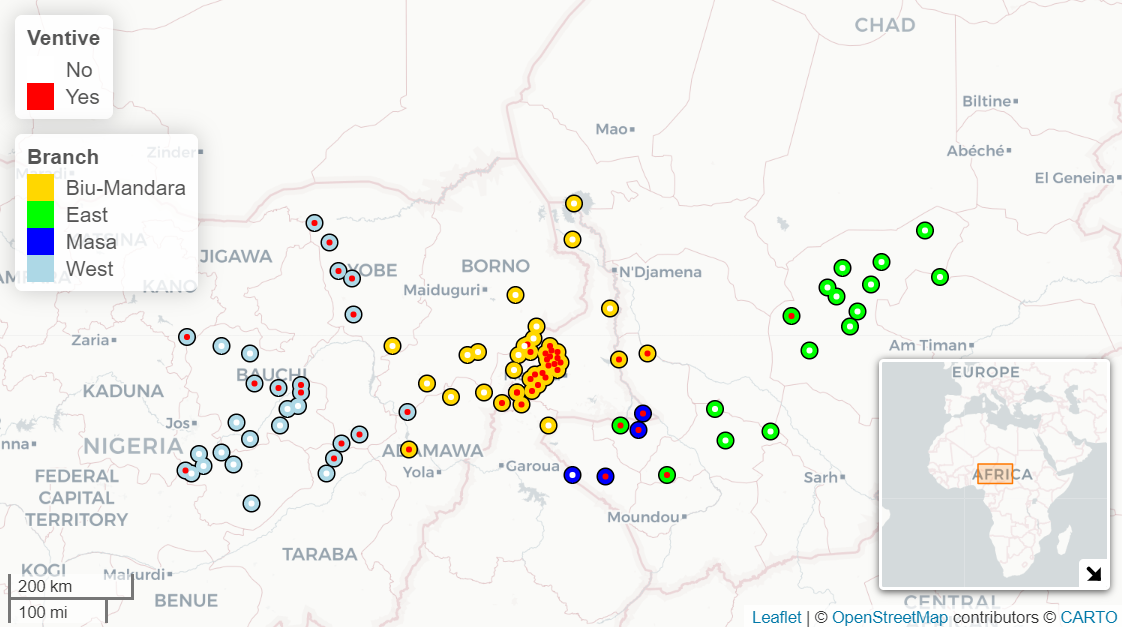
\includegraphics[width=\textwidth]{maps/ventive.png}
	\caption{Map of ventive directional extensions in Chadic languages}
	\label{fig:ventivemap}
\end{figure}



In the West branch, ventive extensions are the only attested type of directional extension and are found in 15 of the 29 West Chadic languages in the sample. Most of the examples of ventive extensions in West Chadic languages are from the West Chadic A group.\footnote{One additional West Chadic A language, \hyperref[beel]{Beele}, is said to have ventive extensions \citep[21]{schuhBoleTangaleLanguagesBauchi1978}, but it is not counted here since no examples are given to support the analysis.} Within the West Chadic B group, only two languages have evidence of a ventive extension. These are both part of the West B1 subgroup and are spoken in the northern part of Nigeria (Yobe State) in an area quite far from other West B languages. \citet[308]{schuhChadicCornucopia2017} states that there are no traces of directional extensions in West Chadic B2 or West Chadic B3.\footnote{\citet[]{schuhChadicCornucopia2017} uses the label \textit{West Chadic C} for West Chadic B3.} If this is correct, the distinction between West A and West B is even more stark than indicated in Table \ref{tab:ventive}. It is plausible that all West Chadic ventive directional extensions are cognate forms, but this cannot be extended to establish a historical relationship with ventive extensions in other branches (Chapter \ref{ch:diachrony}).

Among Biu-Mandara languages, 26 of 42 have a ventive extension (62\%). Ventive extensions are most common among the Biu-Mandara South subgroup (10 of 13). Within this subbranch, all six Dabaic languages have a ventive form that could be reconstructed as  $^\ast$\textit{-aha}. In the Biu-Mandara North subbranch, ventive extensions are not uncommon, found in 14 of 27 languages, but with a variety of forms. There is an areal dimension to the distribution of ventive extensions in North Biu-Mandara languages. As shown in the map in Figure \ref{fig:ventivemap}, there is a dense cluster of Biu-Mandara languages spoken in the area between the city of Maroua and the Mandara mountain range on the Cameroon-Nigerian border. The Biu-Mandara North languages spoken in this area all have a ventive extension. The North Biu-Mandara languages found to the west and north of this area do not have ventive extensions. 

Three of the four Masa languages in the sample have ventive extensions. The North Masa languages have similar suffixes featuring a palatal approximant, but the ventive extension \textit{-fi} in the South Masa language Herdé cannot be assumed to be a cognate form. 

Compared to other branches, there is a significant bias against ventive extensions in East Chadic languages with such morphemes attested in less than 20\% of languages (three of 16).\footnote{By binomial test, the rate of three of 16 is significantly lower than the rate of 47 of 91 languages (52\%) overall for all Chadic branches (p < 0.01).} Keeping in mind the limited data available for the East Chadic A group of languages (descriptions are available for only five of 15 languages), it appears that ventive extensions may be relatively common there compared to the East Chadic B subgroup (the easternmost cluster of Chadic languages) which stands out as having very few instances of ventive extensions attested (or any directional extensions at all). The two East Chadic A languages with directionals are spoken in the same geographical area as Masa languages, so language contact is a possible explanation for the appearance of directional extensions in these languages. This area is not far east of the dense cluster of Biu-Mandara languages with a ventive extension discussed above, as shown on the map in Figure \ref{fig:ventivemap}. 

\section{Itive directional extensions} \label{sec:itive2}

Itive directional extensions are almost exclusively found in Biu-Mandara and Masa languages, as seen in Table \ref{tab:itive}. They are attested in nearly 40\% of Biu-Mandara and Masa languages. No itive extensions are attested in West Chadic languages, and only one case has been identified in East Chadic languages. This strong correlation between subbranches and the presence of itive extensions essentially determines the geographic distribution of itive extensions as well, but it can be observed in the map in Figure \ref{fig:itivemap} that the Biu-Mandara languages spoken furthest north (the Kotoko-Buduma subgroup) do not have itive extensions.

%Data in tab:itive based on number from python script in Itive file
\begin{table}
	\caption{Numbers of Chadic languages with an itive extension}
	\label{tab:itive}
	\begin{tabular}{lrrc} % add l for every additional column or remove as necessary
		\lsptoprule
		Subbranch &  Itive &  	No itive & \% \\
		\midrule
West A            &      0 &        22 &  \bwpie{0}{22} \\
West B            &      0 &         7 &  \bwpie{0}{7}  \\
Biu-Mandara Hurza &      0 &         2 &  \bwpie{0}{2} \\
Biu-Mandara North &     12 &        15 &  \bwpie{12}{15} \\
Biu-Mandara South &      4 &         9 &  \bwpie{4}{9} \\
Masa North        &      2 &         0 &  \bwpie{2}{0} \\
Masa South        &      0 &         2 &  \bwpie{0}{2}  \\
East A            &      1 &         4 &   \bwpie{1}{4}  \\
East B            &      0 &        11 &  \bwpie{0}{11}  \\
\midrule
Total             &     19 &        72 &  \bwpie{19}{72}  \\
		\lspbottomrule
	\end{tabular}
\end{table}

\begin{figure}
	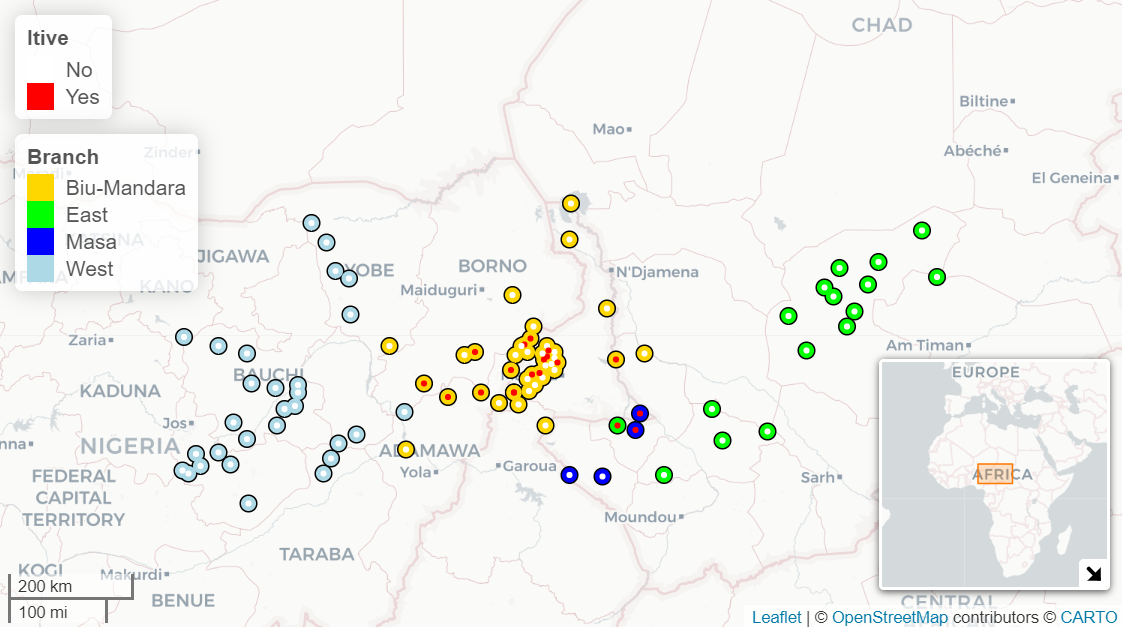
\includegraphics[width=\textwidth]{maps/itive.png}
	\caption{Map of itive extensions in Chadic by branch}
	\label{fig:itivemap}
\end{figure}

The only Chadic language outside of Biu-Mandara and Masa languages to have an itive extension is the East Chadic language \hyperref[kera]{Kera}. The morpheme \textit{-ná} is described as a counterpart of the ventive extension \textit{-dà}, but with distal meaning \citep[115]{ebertSpracheUndTradition1979}. In the few examples Ebert gives, the distal marker is either co-occurring with the totality marker \textit{wə́ra} or appears to have a postpositional function. However, in at least some contexts it is possible for \textit{-na} to appear suffixed to a verb of motion with an itive directional function, as in (\ref{ex:kera7}).  


\ea\label{ex:kera7}
\langinfo{\hyperref[kera]{Kera} verb \textit{kə́láŋ} ‘enter' with itive marker}{}{p.c., Jackie Hainaut} \\
\gll kə́láŋ-na	\\
enter-\gl{itive}	\\
\glt `went in'
\z 

%\subsection{Comparing ventive and itive extensions}

Given the complementary meanings of the itive and ventive extensions, it would be reasonable to expect some type of correlation between the presence of these two functions in particular languages. Table \ref{tab:directionals} shows that the ventive extension appears more frequently, in 47 languages, compared to the itive extension which appears in 19 languages. The higher frequency of ventive extensions follows if there is a default assumption that motion events described without a specific direction generally occur away from the deictic center \citep{wilkinsWhenGOMeans1995}, and therefore it is natural for a language to only specify ventive motion, leaving itive motion unmarked in the verbal morphology. By that line of reasoning, we would expect to find a one-way correlation such that languages are likely to have a grammaticalized ventive marker without having a grammaticalized itive marker, but not vice versa. This is, of course, the only possible pattern in West and East Chadic languages where itive extensions are absent. Among Biu-Mandara and Masa languages it is, as expected, more common to find languages with only a ventive extension than it is to find languages with only an itive extension, as shown in Figure \ref{fig:ventiveitivepie}. 17 languages have only a ventive extension with no itive extension, and 12 languages have both a ventive extension and an itive extension. However, there are six languages where an itive extension is attested, but not a ventive extension. Five of the six languages with an itive extension but no (attested) ventive extension are of the North Biu-Mandara subbranch and are geographically close to each other (\hyperref[bura]{Bura}, \hyperref[glav]{Glavda}, \hyperref[huba]{Huba}, \hyperref[marg]{Margi}, \hyperref[psik]{Psikye}).\footnote{In the case of \hyperref[psik]{Psikye}, \citet[113--114]{smithKapsikiLanguage1969} describes a verbal suffix \textit{-ke} which has a ventive subsequent motion interpretation with non-motion verbs, but no examples are given of this suffix with a motion verb. In the closely related \hyperref[bana]{Bana} language, there is a ventive extension \textit{-ke}, suggesting that Psikye likely does have a ventive extension which is yet unattested in the available data. \hyperref[gaan]{Ga'anda} is described as having an itive directional extension (and no ventive), but the same situation is found in the closely related language \hyperref[tera]{Tera} where there is enough evidence to consider the itive directional an adverb rather than a verbal extension.} In summary, it is fairly common to find an asymmetry in which languages have a ventive extension but no itive extension. The opposite asymmetry is less common.

%number in fig:ventiveitivepie are from python code in file VentItive
\begin{figure}
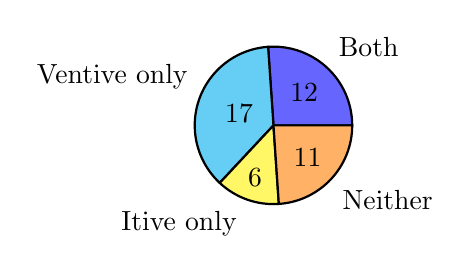
\begin{tikzpicture}
		\pie[radius = 1, sum = auto]{12/Both,
			17/Ventive only,
			6/Itive only,
			11/Neither}	
	\end{tikzpicture}
	\caption{Ventive and itive extensions in Biu-Mandara and Masa languages}
	\label{fig:ventiveitivepie}
\end{figure}

%\begin{figure}
%	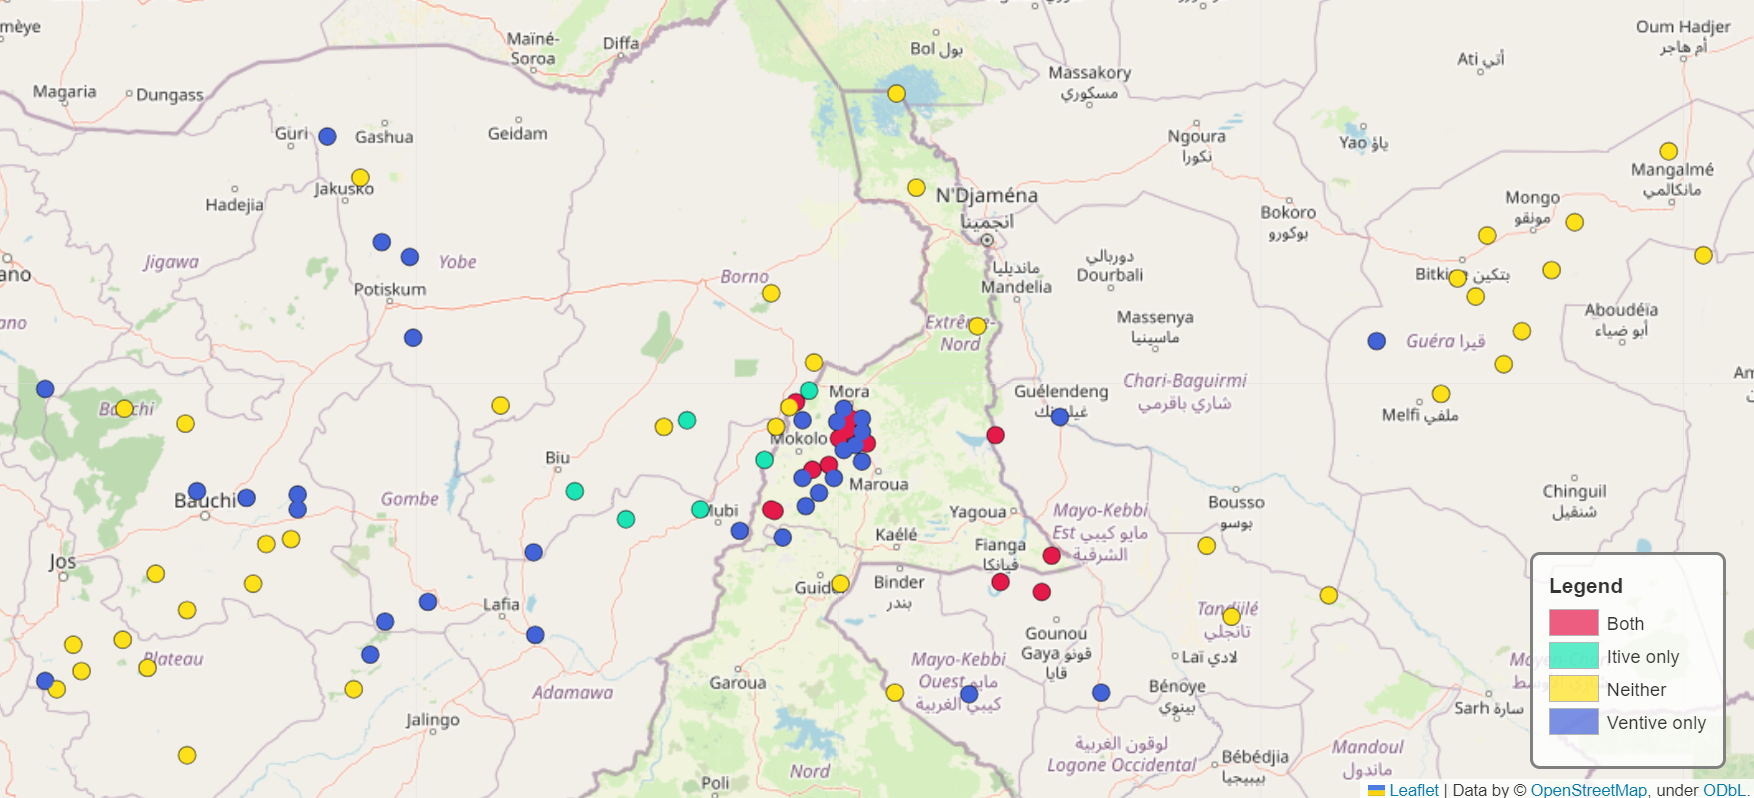
\includegraphics[width=\textwidth]{maps/ventive_itive.png}
%	\caption{Map of intersection of ventive and itive extensions in Chadic}
%	\label{fig:ventiveitivemap}
%\end{figure}	

\section{Boundary-crossing directional extensions} \label{sec:bounded2}

%\begin{figure}[h!]
%	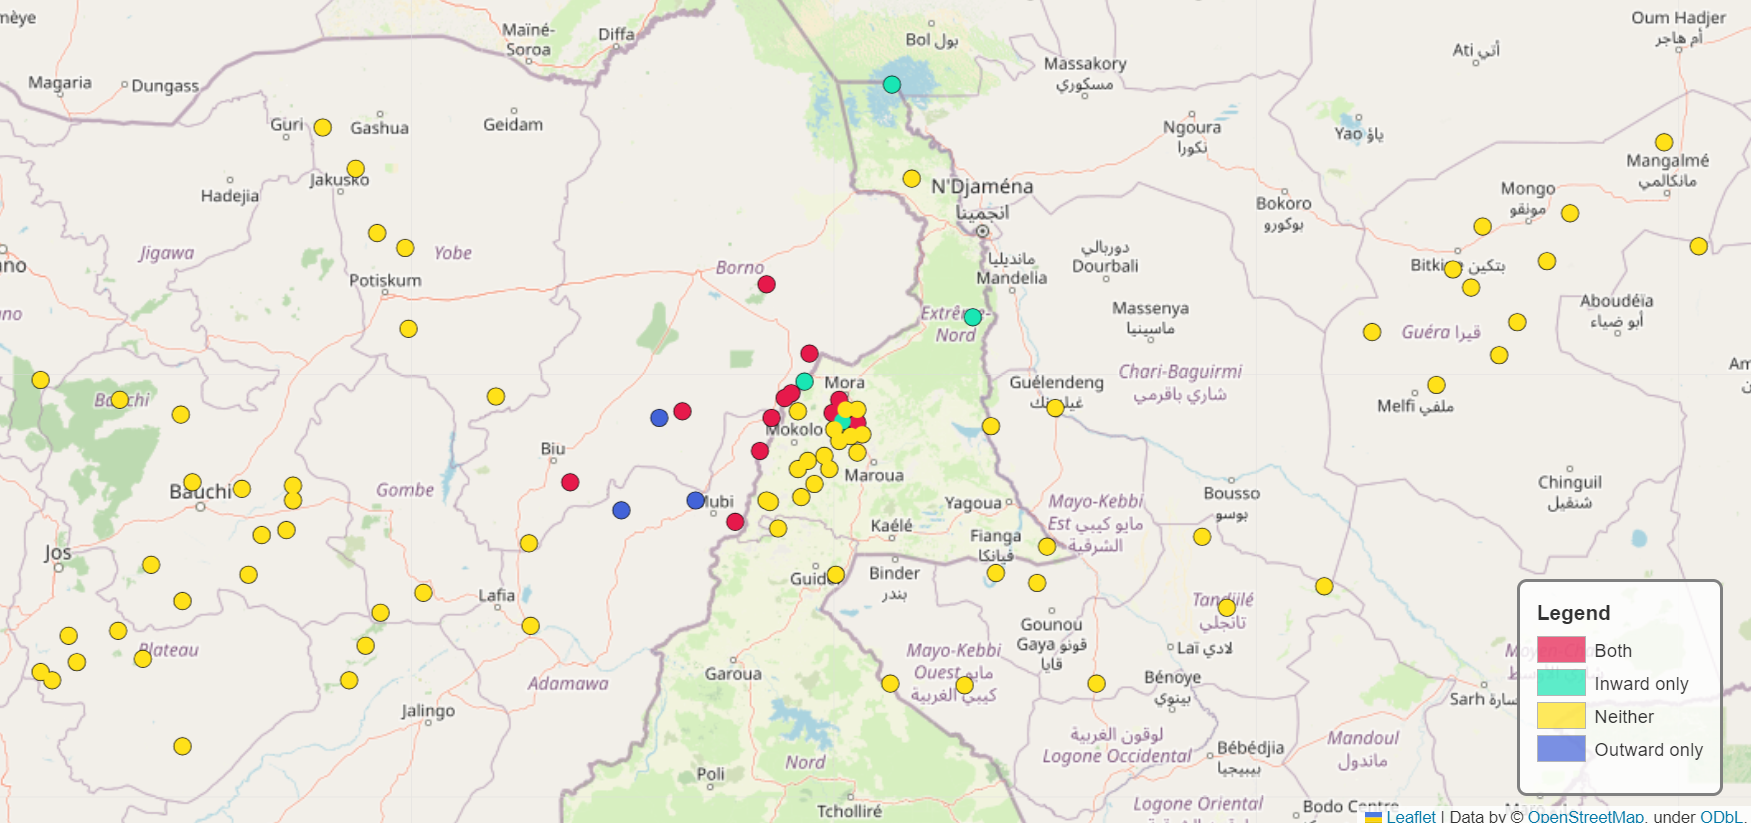
\includegraphics[width=\textwidth]{maps/in_out.png}
%	\caption{Map of boundary-crossing directional extensions in Chadic}
%	\label{fig:inoutmap}
%\end{figure}

Directional extensions expressing inward or outward motion are not as common as ventive or itive extensions. As seen in Table \ref{tab:directionals}, there are 16 languages out of the sample of 91 languages that have an inward extension, and 15 that have an outward extension. Nearly all of these languages are classified as part of the Biu-Mandara North group with only a few Biu-Mandara South languages included, as seen in Table \ref{tab:inward} and Table \ref{tab:outward}. As shown in Figure \ref{fig:inoutpie}, 12 languages have both an inward and an outward extension. Four languages only have an inward extension and three only have an outward extension. %The geographic distribution of boundary-crossing directional extensions in Chadic languages is shown on the map in Figure \ref{fig:inoutmap}.

%Data in tab:inward from python script file Inward 
\begin{table}
	\caption{Number of languages with an inward extension}
	\label{tab:inward}
	\begin{tabular}{lrrc} % add l for every additional column or remove as necessary
		\lsptoprule
		Subbranch &  Inward &  	No inward & \%\\
		\midrule
		West            &       0 &         29  &  \bwpie{0}{29} \\
%		West A            &       0 &         22  &  \bwpie{0}{22} \\
%		West B            &       0 &          7 &  \bwpie{0}{7} \\
		Biu-Mandara Hurza &       0 &          2 &   \bwpie{0}{2} \\
		Biu-Mandara North &      14 &         13 &  \bwpie{14}{13}  \\
		Biu-Mandara South &       2 &         11 &  \bwpie{2}{11} \\
		Masa 		        &       0 &         4 &  \bwpie{0}{4}  \\
%		Masa North        &       0 &         2 &  \bwpie{0}{2}  \\
%		Masa South        &       0 &          2 &   \bwpie{0}{2}  \\
		East            &       0 &          16 &   \bwpie{0}{16} \\
%		East A            &       0 &          5 &   \bwpie{0}{5} \\
%		East B            &       0 &         11 &   \bwpie{0}{11} \\
		\midrule
		Total             &      16 &         75 &   \bwpie{16}{75} \\
		\lspbottomrule
	\end{tabular}
\end{table}

%Data in tab:outward from python script file outward 
\begin{table}
	\caption{Number of languages with an outward extension}
	\label{tab:outward}
	\begin{tabular}{lrrc} % add l for every additional column or remove as necessary
		\lsptoprule
		Subbranch &  Outward &  	No outward & \%\\
		\midrule
West             &        0 &          29 &  \bwpie{0}{29} \\
%West A            &        0 &          22 &  \bwpie{0}{22} \\
%West B            &        0 &           7  &  \bwpie{0}{7} \\
Biu-Mandara Hurza &        0 &           2 &  \bwpie{0}{2} \\
Biu-Mandara North &       12 &          15 &  \bwpie{12}{15}  \\
Biu-Mandara South &        3 &          10 &   \bwpie{3}{10} \\
Masa 		        &       0 &         4 &  \bwpie{0}{4}  \\
%Masa North        &        0 &           2 &  \bwpie{0}{2}  \\
%Masa South        &        0 &           2 &  \bwpie{0}{2} \\
East             &        0 &           16 &  \bwpie{0}{16} \\
%East A            &        0 &           5 &  \bwpie{0}{5} \\
%East B            &        0 &          11 &  \bwpie{0}{11} \\
\midrule
Total             &       15 &          76 &  \bwpie{15}{76} \\
		\lspbottomrule
	\end{tabular}
\end{table}

\begin{figure}
	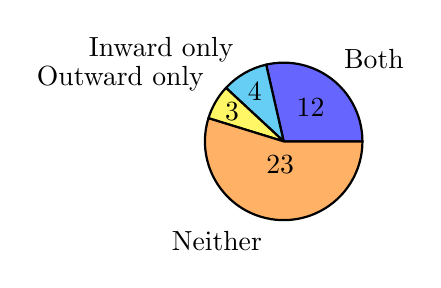
\begin{tikzpicture}
		\pie[radius = 1, sum = auto]{12/Both,
			4/Inward only,
			3/Outward only,
			23/Neither}	
	\end{tikzpicture}
	\caption{Boundary-crossing directional extensions in Biu-Mandara languages}
	\label{fig:inoutpie}
\end{figure}

\newpage
\section{Vertical directional extensions} \label{sec:vertical2}

As shown in Table \ref{tab:directionals}, only eight of the 91 languages in the sample have an upward extension. All of them are Biu-Mandara languages, mostly of the Biu-Mandara North subbranch, as shown in Table \ref{tab:upward}. 

%data in tab:upward from python script in file Upward
\begin{table}
	\caption{Number of Chadic languages with an upward extension}
	\label{tab:upward}
	\begin{tabular}{lrrc} % add l for every additional column or remove as necessary
		\lsptoprule
		Subbranch &  Upward &  	No upward & \% \\
		\midrule
West            &       0 &         29 &  \bwpie{0}{19} \\
%West A            &       0 &         22 &  \bwpie{0}{22} \\
%West B            &       0 &          7 &  \bwpie{0}{7} \\
Biu-Mandara Hurza &       0 &          2 &  \bwpie{0}{2} \\
Biu-Mandara North &       6 &         21 &  \bwpie{6}{21} \\
Biu-Mandara South &       2 &         11 &  \bwpie{2}{11} \\
Masa 		        &       0 &         4 &  \bwpie{0}{4}  \\
%Masa North        &       0 &         2 &  \bwpie{0}{2} \\
%Masa South        &       0 &          2 &  \bwpie{0}{2}\\
East             &         0 &            16&  \bwpie{0}{16} \\
%East A            &       0 &          5 &  \bwpie{0}{5} \\
%East B            &       0 &         11  &  \bwpie{0}{11} \\
		\midrule
Total       &     8 &       83 &  \bwpie{8}{83} \\
		\lspbottomrule
	\end{tabular}
\end{table}

A slightly higher number of languages, 13, have a downward extension. Again, all of these are Biu-Mandara languages, mostly of the Biu-Mandara North subbranch, as shown in Table \ref{tab:downward}. 

%data in tab:downward from python script in file Downward
\begin{table}
	\caption{Number of Chadic languages with a downward extension}
	\label{tab:downward}
	\begin{tabular}{lrrc} % add l for every additional column or remove as necessary
		\lsptoprule
		Branch &  Downward &  	No downward & \% \\
		\midrule
West            &       0 &         29 &  \bwpie{0}{19} \\
%West A            &         0 &           22&   \bwpie{0}{22}\\
%West B            &         0 &            7 &   \bwpie{0}{7} \\
Biu-Mandara Hurza &         0 &            2 &  \bwpie{0}{2} \\
Biu-Mandara North &        10 &           17 &  \bwpie{10}{17}\\
Biu-Mandara South &         3 &           10 &  \bwpie{3}{10} \\
Masa 		        &       0 &         4 &  \bwpie{0}{4}  \\
%Masa North        &         0 &            2 &  \bwpie{0}{2} \\
%Masa South        &         0 &            2 &  \bwpie{0}{2} \\
East             &         0 &            16&  \bwpie{0}{16} \\
%East A            &         0 &            5&  \bwpie{0}{5} \\
%East B            &         0 &           11 &  \bwpie{0}{11} \\
\midrule
Total             &        13 &           78&  \bwpie{13}{78} \\
		\lspbottomrule
	\end{tabular}
\end{table}

Chadic languages are more likely to have a downward extension without an upward extension than vice versa, as shown in Figure \ref{fig:updownpie}. Seven languages have both downward and upward extensions, six languages have only a downward extension, and just one language, \hyperref[malg]{Malgwi}, has an upward extension without also having a downward extension. 

\begin{figure}
	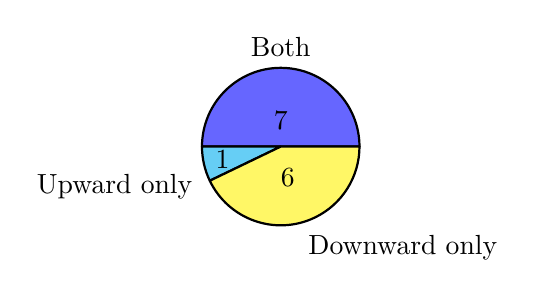
\begin{tikzpicture}
	\pie[radius = 1, sum = auto]{7/Both,
		1/Upward only,
		6/Downward only}	
\end{tikzpicture}
	\caption{Chadic languages with upward and/or downward extensions}
	\label{fig:updownpie}
\end{figure}

%The geographic distribution of vertical extensions is shown in Figure \ref{fig:updownmap}. 
Languages with vertical extensions are clustered around the Nigeria-Came\-roon border, precisely where the Mandara mountain range is located. While the correlation between vertical extensions and a mountainous environment is striking, it should be emphasized that other Chadic languages are spoken in mountainous areas without having developed any vertical directional extensions. The mountains of the Guera Massif in central Chad, where many East Chadic languages are spoken, and the Jos Plateau, where many West Chadic languages are spoken, are of similar elevation to the Mandara mountains.

%\begin{figure}
%	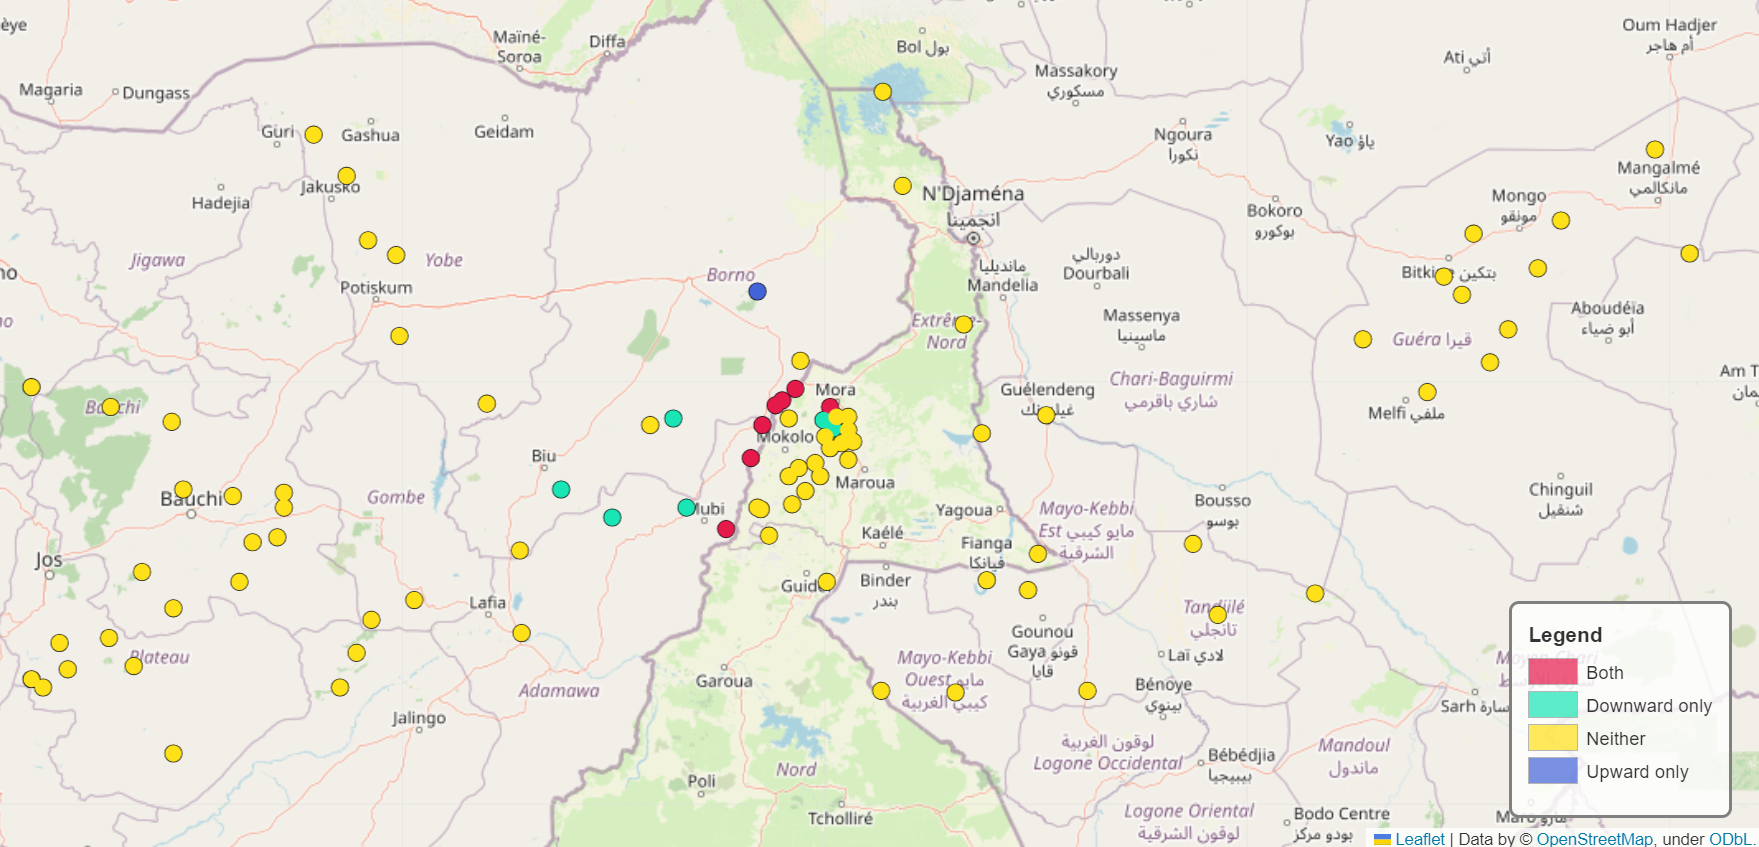
\includegraphics[width=\textwidth]{maps/up_down.png}
%	\caption{Map of upward and downward extensions in Chadic}
%	\label{fig:updownmap}
%\end{figure}

\section{Directional extensions `onto' and `under'}  \label{sec:onto2}

There are nine languages with an `onto' directional extension, as indicated in Table \ref{tab:directionals} above. All nine of these languages are in the Biu-Mandara North subbranch, and all but one are in the Margi-Mandara-Mofu group. The three languages with an `under' directional extensions are all Mandaraic languages (Biu-Mandara North). The forms of these extensions, shown in Table \ref{tab:under}, all share a segment \textit{s}, suggesting that they are cognate forms (Chapter \ref{ch:diachrony}).

%The geographic distribution of the nine languages with an `onto' extension is shown in Figure \ref{fig:ontomap}.

%\begin{figure}
%	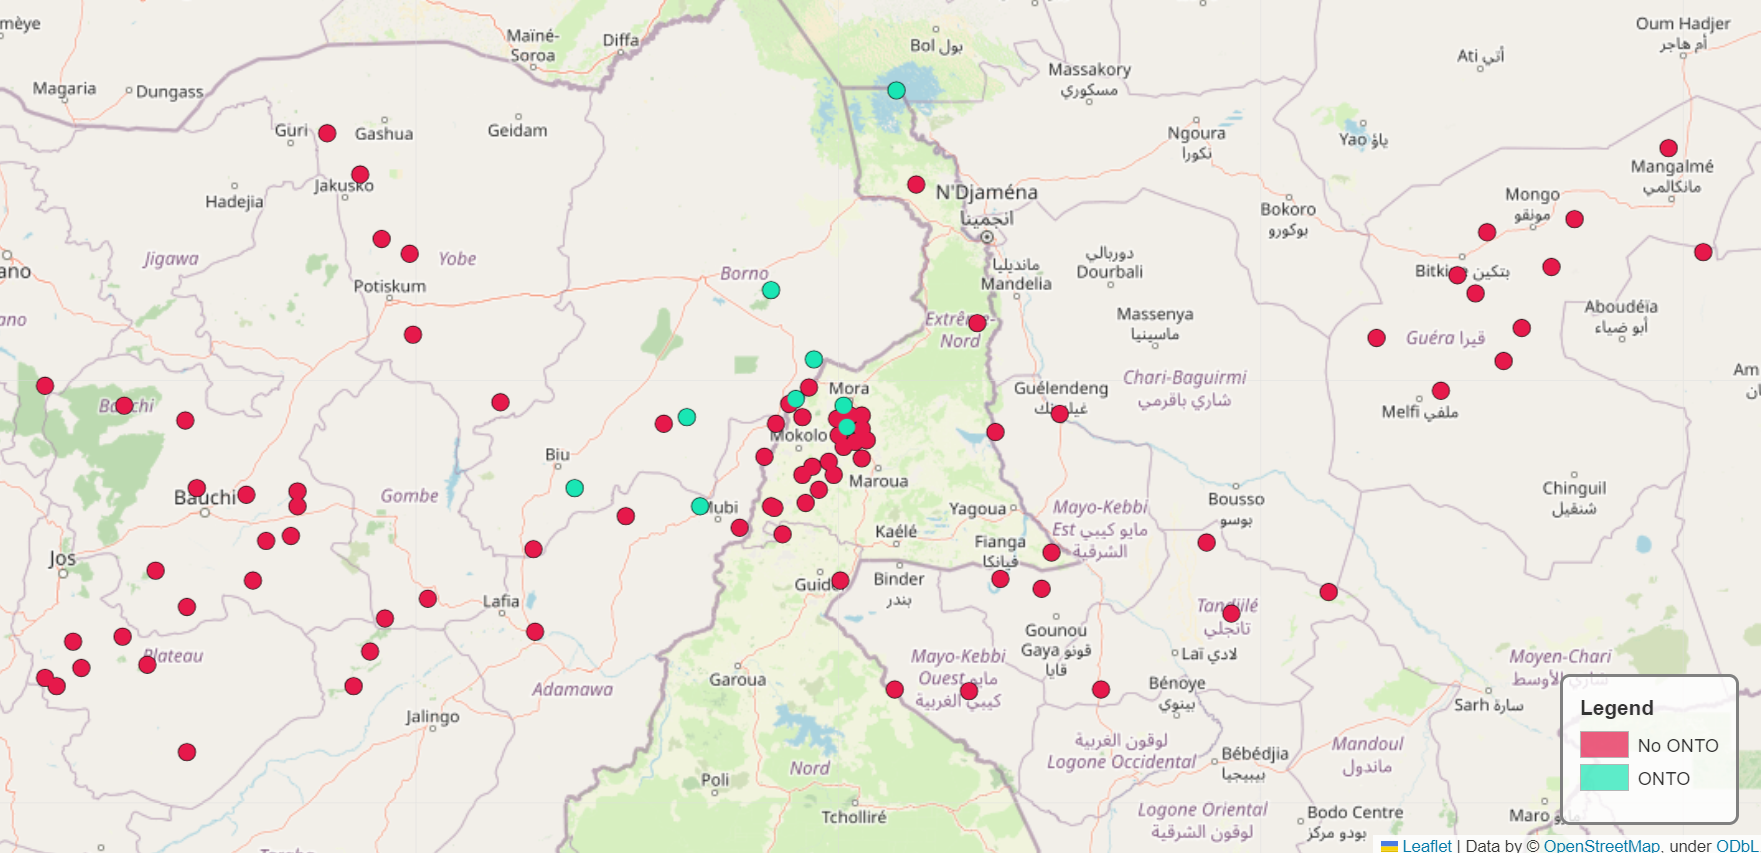
\includegraphics[width=\textwidth]{maps/onto.png}
%	\caption{Map of `onto' extensions in Chadic}
%	\label{fig:ontomap}
%\end{figure}

\begin{table}
	\caption{Forms of `under' extensions in Mandaraic subgroup}
	\label{tab:under}
	\begin{tabular}{ll}
		\lsptoprule
	Language	&     Form    \\ %&  Group & Subgroup         \\
		\midrule
%		\hyperref[bura]{Bura} & \textit{kəra}, \textit{nkir} ? & M.-M.-M. & Bura-Margi \\
		\hyperref[dghw]{Dghwede} & \textit{sege} \\ %& Margi-Mandara-Mofu & Mandaraic \\
		\hyperref[park]{Parkwa}	 & \textit{asə} \\ %& M.-M.-M. & Mandaraic \\
		\hyperref[glav]{Glavda} &	\textit{s}	\\ %&	M.-M.-M.	& Mandaraic \\	
		\lspbottomrule
	\end{tabular}
\end{table}

\section{Co-occurrence of directional extensions in particular languages} \label{sec:co-occurrence}

The above sections examined how frequently each particular semantic type of directional extension is attested across a sample of Chadic languages. This section looks at how many semantic types of directional extensions co-occur in a particular language. The directional meanings considered are the eight discussed in the above sections.\footnote{If including the more rarely attested semantic types, \hyperref[psik]{Psikye} also has a bushward extension bringing its total up from five to six, \hyperref[lama]{Lamang} also has a homeward extension bringing its total up from four to five, and Bura has both a homeward and a `side' extension bringing its total up from five to seven. } The number in the first column of Table \ref{tab:multiple} is the number of these eight directional meanings that are expressed through a verbal extension in a particular language, from zero up to eight. The remaining columns indicate how many languages of each branch of Chadic languages have that number of directional meanings attested in verbal extensions.\footnote{A direct comparison of Table \ref{tab:multiple} with Table \ref{tab:dirmorphs} shows a discrepancy in the row labeled `1'. This is because \hyperref[kana]{Kanakuru} has two directional extensions (post-verbal \textit{-tə(ru)} and pre-verbal \textit{bo}) which are each counted as separate morphemes in Table \ref{tab:dirmorphs}, but both directional extensions express the same meaning, ventive, and so are only counted once in Table \ref{tab:multiple} which tabulates how many of the main eight types of directional meaning each language can express.} 

%Data in tab:multiple is from python script in Number file 
\begin{table}
	\caption{Number of directional meanings expressed}
	\label{tab:multiple}
	\begin{tabular}{rrrrrc}
		\lsptoprule
{} &  West &  Biu-Mandara &  Masa &  East &  Total \\
\midrule
0 &    14 &            3 &     1 &    13 &     31 \\
1 &    15 &           14 &     1 &     2 &     32 \\
2 &     0 &            9 &     2 &     1 &     12 \\
3 &     0 &            3 &     0 &     0 &      3 \\
4 &     0 &            5 &     0 &     0 &      5 \\
5 &     0 &            6 &     0 &     0 &      6 \\
6 &     0 &            0 &     0 &     0 &      0 \\
7 &     0 &            1 &     0 &     0 &      1 \\
8 &     0 &            1 &     0 &     0 &      1 \\
%Including SIDE, BUSH, HOME
%0 &    15 &            3 &     1 &    13 &     32 \\
%1 &    14 &           14 &     1 &     2 &     31 \\
%2 &     0 &            9 &     2 &     1 &     12 \\
%3 &     0 &            3 &     0 &     0 &      3 \\
%4 &     0 &            4 &     0 &     0 &      4 \\
%5 &     0 &            5 &     0 &     0 &      5 \\
%6 &     0 &            1 &     0 &     0 &      1 \\
%7 &     0 &            2 &     0 &     0 &      2 \\
%8 &     0 &            1 &     0 &     0 &      1 \\
		\lspbottomrule
	\end{tabular}
\end{table}

Over half of the languages with a directional extension (32 of 60) have only one of the eight main semantic types of directional extension, as seen in Figure \ref{fig:multiple}. All but two of these are languages with a ventive directional extension. The others are \hyperref[lagw]{Lagwan} (only inward) and \hyperref[ciba]{Cibak} (only outward).\footnote{In a description of \hyperref[ciba]{Cibak}, \citet{hoffmannZurSpracheCibak1955} mentions a second directional extension, \textit{-nta}. However, the examples given do not substantiate the putative itive directional meaning of this extension.} Twelve languages have two types of directional extensions. Nearly all of these include ventive and itive directional meaning with the sole exception of \hyperref[budu]{Buduma} (inward and `onto'). 

\begin{figure}
	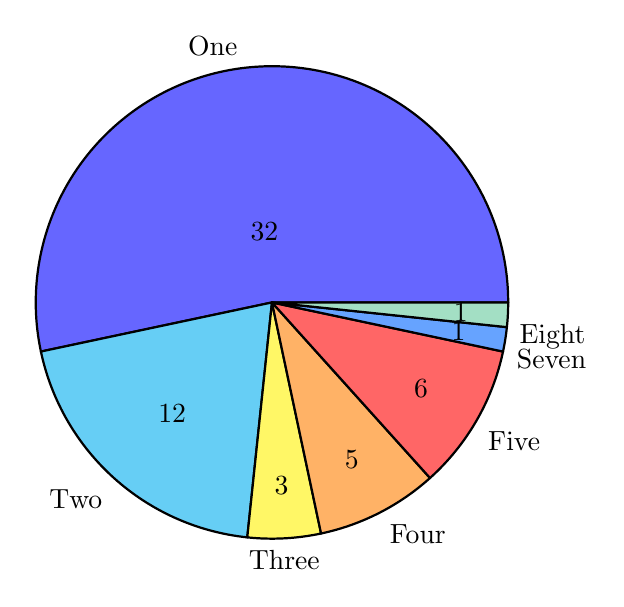
\begin{tikzpicture}
	\pie[radius = 3, sum = auto]{
		32/One,
		12/Two,
		3/Three,
		5/Four,
		6/Five,
		1/Seven,
		1/Eight}	
\end{tikzpicture}
	\caption{Number of directional meanings expressed in verbal extensions}
	\label{fig:multiple}
\end{figure}

In the 16 languages with more than two directional extensions, the ventive type is much less common. Only six of these 16 languages have a ventive extension. In languages with just one or two directional extensions, the ventive appears in 41 of 44 cases. Therefore, there is no implicational hierarchy such that the presence of one type of directional extension entails the existence of another type in the same language (at least from a synchronic perspective). 

Why are ventive extensions ubiquitous in languages with just one or two directional extensions, and much less common in languages with more than two directional extensions? One potential explanation for this pattern may be that there are cognitive motivations for not needing a ventive marker in a more complex system of directional extensions. The other directional extensions provide a rich set of directional notions that render the ventive meaning superfluous. Alternatively, from a diachronic perspective, it could be hypothesized that languages with more directional extensions have developed over an extended period of time, and that during this timespan erstwhile ventive directional extensions have shifted to another function. 

The hypothesis that some ventive forms have undergone reanalysis would be supported if languages without ventive extensions can be shown to have cognate extensions with other functions. For example, \hyperref[bura]{Bura} and \hyperref[marg]{Margi} are languages with multiple directional extensions but no ventive extension. Both languages have an inward extension of the form \textit{-wa}. Could this inward extension be historically related to the ventive extension \textit{-awa} found in other languages of the same subgroup of Margi-Mandara-Mofu languages? More historical reconstruction of each subgroup would be needed to substantiate these types of cognate relationships.

Whereas ventive directional meaning is less common in languages with more directional extensions, conversely, the rarest types of directional extensions (`under', homeward, bushward) are only attested in languages with at least four other types of directional extensions. Diachronically, this suggests that these semantic types have only developed as verbal extensions in languages which already have a robust system of directional extensions including at least some of the inward, outward, upward or downward directional extensions. 

\section{Conclusion} \label{sec:sumdir}

\citet[148]{creisselsAfricaMorphosyntacticArea2008} report that directional morphemes attached to the verb ``are not very common in African languages in general, but they are common in Nilo-Saharan languages.'' While not all verbal extensions in Chadic languages are affixes, it is still reasonable to say that directional verbal morphology is also common in Chadic languages, as the majority of Chadic languages have at least one verbal extension with a directional function, of which most are suffixes. 

The most common directional meaning among Chadic verbal extensions is ventive, toward the deictic center. This is the only type of directional meaning found in verbal extensions across all four branches of Chadic languages. Ventive directionals are also commonly found in the more distantly related Berber languages \citep{mettouchiGrammaticalizationDirectionalClitics2011}. Biu-Mandara languages have innovated beyond ventive meaning and added several other types of directional meaning to their inventory of verbal extensions. Most often, the meanings added are itive, inward, outward, upward and downward. In a global sample of directional morphemes in 114 languages, Ross finds ventive, itive, upward and downward motion to be the most common semantic types. Vertical directional extensions are found in 14 Chadic languages out of 59 Chadic languages with directional extensions (24\%). This is significantly lower than the global average from Ross' sample in which vertical directional semantics are found in 50 of 114 languages with directional morphemes (44\%).\footnote{By binomial test, the rate of 14 of 59 is significantly lower than the rate of 44\% in Ross' sample (p < 0.001). \citet[279]{rossPseudocoordinationSerialVerb2021} also examines the linear order of directional verbal morphology and the verb it modifies. The results are that directional morphology is post-verbal in 59\% of the sample. All directional morphology in Chadic languages is post-verbal with the exception of the \hyperref[kana]{Kanakuru} auxiliary \textit{bo} \citep[76]{newmanKanakuruLanguage1974}.} In Chadic languages that have multiple directional extensions, less common directional meanings are found, such as `onto' and `under', as well as homeward and bushward. This matches the global pattern in which less common types of directional meaning typically occur in languages that have a larger number of directional morphemes \citep[278]{rossPseudocoordinationSerialVerb2021}. 

\citet{bickelTypology21stCentury2007} describes linguistic typology as answering the multipart question ``What’s where why?'' As summarized above, this chapter has provided a robust response to the \textit{what} and \textit{where} questions of directional extensions in Chadic languages. Answering the \textit{why} question is an even more challenging task, and it ultimately cannot be fully addressed without expanding beyond Chadic languages to examine the genetic context of Afro-Asiatic languages and the areal context of the highly multilingual and linguistically diverse environments in which the Chadic languages are spoken. One step toward that goal in future research will be to construct a theory of \textit{how} Chadic languages came to be the way they are in the sense of understanding what the major processes of historical change have been. A historical reconstruction is not the main goal of this research, but the available evidence gleaned from the comparative synchronic picture is presented in Chapter \ref{ch:diachrony} awaiting further investigation when possible. 

\chapter{Diachrony of directional extensions} \label{ch:diachrony} 

This chapter compiles the available evidence for how directional extensions have developed historically in Chadic languages. Historical reconstruction has been a focus for many early scholars of Chadic languages, but beyond the general internal structure of the family proposed by \citet{newmanChadicClassificationReconstructions1977}, there has only been limited progress in developing an overall picture of the history of these languages. In the assessment of \citet[343--344]{guldemannHistoricalLinguisticsGenealogical2018}, ``the reconstructions [of lexical forms]... are not established transparently in a bottom-up procedure within a clear phylogenetic structure, and only a limited number of them involve the level of the proto-language'' and in regard to grammaticalized morphemes ``hardly any domain has received such a depth of research as to produce a concrete set of morphological proto-forms that are based either on subgroup reconstructions or, given the size of the family, at least on a representative language sample.''

\section{Previous reconstructions of directional extensions}

In regard to directional extensions, there have been a few proposals. \citet[275]{newmanChadicExtensionsPredative1977} claims that ventive extensions ``can be reconstructed for Proto-Chadic with a high degree of certainty.'' Two forms are reconstructed, each based on data from three West Chadic languages and three Biu-Mandara languages. Newman proposes that neither of these forms had a ventive function in Proto-Chadic. The proto-form $^\ast$\textit{(a)wa} is proposed to have been a distal demonstrative and the proto-form  $^\ast$\textit{in} is proposed to have been a benefactive marker.\footnote{Both distal location and benefactive meanings are co-expressed with ventive directionals in Chadic languages (Chapter \ref{ch:functions}, Sections \ref{sec:ventloc} and \ref{sec:beneficiary}), but it is unclear why the path of grammaticalization should be from location and beneficiary to ventive direction rather than the other way around. Since reflexes of Newman's ``distal'' $^\ast$\textit{(a)wa} can also express benefactive meaning, Newman suggests that the path of grammaticalization actually goes both ways. Not only can a benefactive marker become a ventive marker, but (a distal marker that becomes) a ventive marker can also become a benefactive marker.} It is left unexplained why many West Chadic languages have reflexes of both of these forms as aspect-related allomorphs. 

%\footnote{``The original meaning of the Distant extension would have been to indicate that the action of the verb was done ``there'' at some distance from the speaker... was probably entirely locative in nature'' \citep[276]{newmanChadicExtensionsPredative1977}.} 
%\footnote{``The primary meaning of this extension was to indicate that the action of a verb was destined for, done for the benefit of, or otherwise affected or pertained to someone'' \citep[281]{newmanChadicExtensionsPredative1977}.} 

\citet{frajzyngierVentiveCentrifugalChadic1987} takes a step forward by increasing the sample to 24 languages with ventive (and itive) directional extensions. Frajzyngier takes a more conservative approach by not proposing Proto-Chadic forms. For West Chadic ventive forms, the aspect-related allomorphy is explained by positing that these verbal extensions are derived from verbs in a directional multiverb construction. Frajzyngier notes that the forms of ventive and itive extensions in Biu-Mandara do not match the West Chadic forms and suggests that there may have been a variety of sources for directional extensions in Biu-Mandara in addition to the possible grammaticalization of verbs. The particular reconstructions proposed do not hold up to further scrutiny,\footnote{For example, \citet[35]{frajzyngierVentiveCentrifugalChadic1987} gives possible verbal sources of three itive directional extensions, but \hyperref[marg]{Margi} \textit{-ba} is an outward extension, \hyperref[musg]{Musgu} (Munjuk) \textit{-fu} was not found in other sources, and \hyperref[lagw]{Lagwan} \textit{-li} is an inward extension. \citet{heineWorldLexiconGrammaticalization2002} unfortunately refer to Frajzyngier's Lagwan data as an example of grammaticalization from a verb `go' to an itive directional marker. They also cite an example Frajzyngier gives from Hwana (hwan1240) but this data is from unpublished fieldnotes and cannot be verified.} but the key contribution of this paper is to observe that widespread use of ventive directional extensions does not necessarily entail a common etymological source, especially given the absence of cognate forms across branches of Chadic languages. 

\citet[306--318]{schuhChadicCornucopia2017} also recognizes the differences between directional extensions in each branch of Chadic languages. Three consonants are suggested as proto-forms of ventive directional extensions in West Chadic languages:  $^\ast$\textit{-w}, $^\ast$\textit{-n}, and $^\ast$\textit{-t}. Schuh tentatively suggests that these proto-forms may have shifted to other functions in Biu-Mandara languages, but largely concludes that Biu-Mandara languages ``share an areal feature of having developed complex systems of directional verbal extensions through reinterpretation and grammaticalization of verbs, nouns, adverbs, and prepositions'' \citep[316]{schuhChadicCornucopia2017}.\footnote{Schuh excludes the Kotoko-Buduma and Musguic languages from this description as part of his proposed ``Central Chadic B'' group.} 

\begin{figure}[t]
	\begin{forest}
		forked edges, for tree={grow=0,edge=thick, s sep=-4pt, anchor=base west,  font=\strut\footnotesize\sffamily, grow'=east} % s sep=0pt,
		[West Chadic  
		[A 
		[A1 [Hausa \textit{ō},fill={white!50!yellow}, tier=language] ]
		[A2 
		[Boleic 
		[Karekare \textit{(n)ee, tu} ,fill={white!50!yellow}, tier=language]
		[Beele \textit{u},fill={white!50!yellow}, tier=language]
		[Bole \textit{n, tV, aakoo},fill={white!50!yellow}, tier=language]
		[Geruma \textit{ìŋ},fill={white!50!yellow}, tier=language]
		[Giiwo \textit{(í)n, o},fill={white!50!yellow}, tier=language]
		[Ngamo \textit{no, n, t},fill={white!50!yellow}, tier=language]
		[Bure \textit{ín},fill={white!50!yellow}, tier=language]
		[Gera /L tone/, tier=language]
		[\textit{None} {(Nyam, Galambu)}, tier=language]
		]
		[Tangalic 
		[Kanakuru \textit{tə(ru), bo},fill={white!50!yellow}, tier=language]
		[Kushi \textit{na, ru},fill={white!50!yellow}, tier=language]
		[Pero \textit{na, tu},fill={white!50!yellow}, tier=language]
		[Tangale \textit{tu, na},fill={white!50!yellow}, tier=language]
		]
		]
		[A3 
		[\textit{None} {(Goemai, Mupun, Ngas)}]
		]
		[A4 
		[\textit{None} {(Fyer, Kulere, Ron-Daffo)}]
		[Ron-Scha \textit{ó} ,fill={white!50!yellow}]
		]
		] 
		[B 
		[B1 
		[Bade \textit{àawo, ìina} ,fill={white!50!yellow}]
		[Ngizim \textit{ay, iina} ,fill={white!50!yellow}]
		]
		[B2 
		[\textit{None} ({Pa'a, Miya})]
		]
		[B3 
		[\textit{None} ({Guruntum, Dass, Zaar})]
		]
		] 
		]
	\end{forest}
	\caption{Ventive forms in West Chadic} \label{fig:westventive}
\end{figure}

\section{Ventive}

Following previous work which has not established links between ventive directional extensions across the branches of Chadic languages, the history of directional extensions is discussed separately here for each branch. 

\subsection{West Chadic}

Nearly all ventive forms in West Chadic languages resemble at least one of the three proposed reconstructions, $^\ast$\textit{-w}, $^\ast$\textit{-n}, and $^\ast$\textit{-t}, as marked in yellow in Figure \ref{fig:westventive}. One outlier is \hyperref[gera]{Gera} where ventive direction is expressed by a low tone. \citet[309]{schuhChadicCornucopia2017} does not identify any source of ventive morphemes in West Chadic languages and assumes that languages without a ventive extension have lost this marker, or its function and form have changed beyond recognition. To support this hypothesis, more research is needed into whether West Chadic languages without ventive extensions show evidence of erstwhile ventive extensions that have shifted into another function. The alternative proposal, suggested by \citet{frajzyngierVentiveCentrifugalChadic1987}, is that ventive directional extensions developed from directional multiverb constructions. This leaves open the possibility that this innovation occurred after West Chadic languages split off and did not necessarily occur in all West Chadic languages (e.g., A3, B2, B3). The path of grammaticalization from ventive verb to ventive directional marker is attested in various languages around the world \citep[85--86]{heineWorldLexiconGrammaticalization2002}. However, the reconstruction of this ventive verb root is much less certain. Frajzyngier's proposal assumes a Proto-Chadic verb $^\ast$\textit{wat} as the source, but this is a very speculative reconstruction. Many West Chadic languages (and Biu-Mandara) languages have a motion verb beginning with \textit{w} or \textit{nd}/\textit{d}/\textit{dz}; however, these are most often itive or general motion verb roots (not ventive).  

\subsection{Biu-Mandara and Masa}

\begin{figure}[t]
	\begin{forest}
		forked edges, for tree={grow=0,edge=thick, s sep=-2.5pt, anchor=base west,  font=\strut\footnotesize\sffamily, grow'=east} % s sep=0pt,
		[Biu-Mandara
		[North 
		[Gidar [\textit{None} (Gidar)] ]
		[Higic 
		[Bana \textit{ke} ,fill={white!50!lightgray}]
		[Psikye \textit{ke}? ,fill={white!50!lightgray}]
		]
		[Kotoko-Buduma 
		[\textit{None} ({Buduma, Lagwan, Makary Kotoko})]
		]
		[Lamang-Hdi [\textit{None} (Lamang) ] ]
		[Ma.-Ma.-Mo.	 
		[Bura-Marghi
		[\textit{None} ({Bura, Cibak, Margi, Huba}), tier=language]
		]
		[Mandaraic
		[Dghwede	\textit{àwá} ,fill={white!50!cyan}, tier=language]
		[Matal	\textit{awâŋ} ,fill={white!50!cyan}, tier=language]
		[Parkwa	\textit{ətsa, atsa}, tier=language]
		[\textit{None} ({Glavda, Malgwa, Wandala}), tier=language]
		]
		[Mofuic
		[Merey	\textit{aw} ,fill={white!50!cyan}, tier=language]
		[Zulgo-Gemzek	\textit{ara, aw, ya} ,fill={white!50!cyan}, tier=language]
		[Mofu-Gudur	\textit{wa} ,fill={white!50!cyan}, tier=language]
		[Mada	\textit{re}, tier=language]
		[Moloko	\textit{alaj}, tier=language]
		[Muyang	\textit{biyu}, tier=language]
		[Wuzlam	\textit{ārá}, tier=language]
		]
		]
		[Maroua [North Giziga	\textit{áwà, óò, o} ,fill={white!50!cyan}] ]
		[Musguic 
		[Musgu	\textit{sí} ,fill={white!20!pink}]
		[Mbara	\textit{sì} ,fill={white!20!pink}]
		]
		]
		]
	\end{forest}
	\caption{Ventive forms in Biu-Mandara North} \label{fig:ventivenorthbm}
\end{figure}

It is not yet possible to reconstruct a ventive form for Biu-Mandara languages. The forms of ventive directional extensions in North Biu-Mandara languages are shown in Figure \ref{fig:ventivenorthbm}. There are several forms similar to West Chadic $^\ast$\textit{awa}, primarily found in Margi-Mandara-Mofu languages. These are marked in blue. The Higic languages have a different form, \textit{ke} (marked in grey), and the Musguic languages have a distinct form \textit{si} (marked in pink). This last form is notably similar to ventive directional verbs in Biu-Mandara languages which often have a single consonant \textit{s} as the verb root. There are also a number of forms that are not clearly cognate with any others. While the widespread use of ventive forms suggest that a ventive of some form was likely present in Proto-North-Biu-Mandara, there is not enough evidence available to construct its archaic form. 

The most common form of the ventive directional extension in Biu-Mandara South language is similar to \textit{aha}, as marked in blue in Figure \ref{fig:ventivesouthbm}. These forms are clearly cognate in Dabaic languages, and possibly in Bataic as well. It is tempting to posit a correspondence between \textit{w} and \textit{h} that would link the Dabiac ventive extensions to those in Biu-Mandara North, but \citet{wolffLexicalReconstructionCentral2023} does not find any evidence of such a reflex. A variant featuring \textit{k} appears in Matakam languages, marked in gray. Further information would be needed to decide whether any form can be reconstructed for all South Biu-Mandara languages. 

\begin{figure}
	\begin{forest}
		forked edges, for tree={grow=0,edge=thick, s sep=-3pt, anchor=base west,  font=\strut\footnotesize\sffamily, grow'=east} % s sep=0pt,
		[Biu-Mandara
		[Hurza 
		[Mbuko	\textit{ay} ,fill={white!50!yellow}]
		[Vamé	\textit{aya, ki} ,fill={white!50!yellow}]
		]
		[North ]
		[South 
		[Bataic [Bacama	\textit{á} ,fill={white!50!cyan}, tier=language]
		[Gude	\textit{ʸà} ,fill={white!50!cyan}, tier=language]
		]
		[Dabaic
		[Buwal\textit{	ā, xā} ,fill={white!50!cyan}, tier=language]
		[Gavar	\textit{(h)à} ,fill={white!50!cyan}, tier=language]
		[Daba	\textit{a, (á)ha} ,fill={white!50!cyan}, tier=language]
		[Mazagway	\textit{aha} ,fill={white!50!cyan}, tier=language]
		[Mbudum	\textit{áhà} ,fill={white!50!cyan}, tier=language]
		[Mina	\textit{á(hà)} ,fill={white!50!cyan}, tier=language]
		]
		[Matakam
		[Cuvok	\textit{ék} ,fill={white!50!lightgray}, tier=language]
		[Mafa	\textit{ká(ɗá)} ,fill={white!50!lightgray}, tier=language]
		]
		[Sukur [\textit{None} (Sakun)] , tier=language]
		[Teraic	[\textit{None} {(Ga'anda, Tera)}] , tier=language]
		]
		]
	\end{forest}
	\caption{Ventive forms in Biu-Mandara South and Hurza}  \label{fig:ventivesouthbm}
\end{figure}

The Hurza languages, marked in yellow in Figure \ref{fig:ventivesouthbm}, have their own form of the ventive directional extension. \citet[11]{gravinaVerbPhraseMbuko2001} points to an adverbial \textit{àhày} `to here -- toward deictic centre' as the source of the \hyperref[mbuk]{Mbuko} ventive suffix \textit{-ay}. The Hurza ventive extensions are similar in form to two of the three Masa languages with a ventive directional extension (\textit{áy} in \hyperref[muse]{Musey} and \textit{ey} in \hyperref[masa]{Masana}) while a different form \textit{fi} is found in the other Masa language, \hyperref[herd]{Herde}. The sporadic distribution of potential cognates within Biu-Mandara and between Biu-Mandara and West Chadic languages makes it unclear if these are distantly related forms or coincidental similarities.

\subsection{East}

The three East Chadic languages with a ventive directional extension all have different forms from each other. The East A language, \hyperref[lele]{Lele}, has the form \textit{yè} which could potentially be explained through contact with Masa languages. In East B, the \hyperref[kera]{Kera} form \textit{dà} and \hyperref[soko]{Sokoro} \textit{ti} both feature coronals stops, and so are not dissimilar to some of the West Chadic forms. However, this is not enough data to justify re-constructing a Proto-Chadic ventive extension.\footnote{Compare, for example, ventive directional markers in Berber languages which also tend to have a coronal stop. These are not considered cognates with Chadic ventive extensions, and likely have a more recent origin developed from demonstratives \citep{mettouchiGrammaticalizationDirectionalClitics2011}.} 

In at least three East Chadic languages, the verb `come' appears to be formed of a verb root `go' plus another morpheme: \textit{ɗe} `go' and \textit{ɗéːna} `come' in \hyperref[kwan]{Kwang}, \textit{há} `go' and \textit{háde} `come' in \hyperref[somr]{Somrai}, \textit{è} `go' and \textit{èjè} `come' \hyperref[lele]{Lele}. In Kwang and Somrai, there is no evidence that the syllable distinguishing `go' and `come' is a suffix, as it does not appear with other verbs. In Lele, the form is used as a ventive suffix elsewhere, while in the form \textit{èjè} `come' there is evidence that it is part of the verb root. Are the forms in Kwang and Somrai evidence of the development of ventive directional extensions in East Chadic, or of their loss which has left behind only fossilized traces of erstwhile verbal morphology?

\section{Itive}

\begin{figure}[b]
\fittable{
	\begin{forest}
		forked edges, for tree={grow=0,edge=thick, s sep=-3pt, anchor=base west,  font=\strut\footnotesize\sffamily, grow'=east} % s sep=0pt,
		[Biu-Mandara
		[North 
		[Gidar [\textit{None} (Gidar)] ]
		[Higic 
		[Bana \textit{ghe} ,fill={white!50!yellow}]
		[Psikye \textit{gu} ,fill={white!50!yellow}]
		]
		[Kotoko-Buduma 
		[\textit{None} ({Buduma, Lagwan, Makary Kotoko})]
		]
		[Lamang-Hdi [\textit{None} (Lamang) ] ]
		[Ma.-Ma.-Mo. 
		[Bura-Marghi
		[Bura \textit{mta} ,fill={white!50!cyan} ]
		[Cibak \textit{nta} ? ,fill={white!50!cyan}]
		[Margi \textit{nà} ,fill={white!50!cyan}]
		[Huba \textit{nà},fill={white!50!cyan} ]
		]
		[Mandaraic
		[Dghwede	\textit{dá} ,fill={white!50!lightgray}]
		[Glavda \textit{d(a)} ,fill={white!50!lightgray} ]
		[\textit{None} {(Parkwa, Malgwa, Wandala, Matal)}]
		]
		[Mofuic
		[Zulgo-Gemzek	\textcolor{red}{\textit{aha}} ]
		[Moloko	\textcolor{red}{\textit{ala}}]
		[Mada	\textit{ro},fill={white!50!lime}]
		[Wuzlam	\textit{ārāy, ə̄rə̄},fill={white!50!lime}]
		[\textit{None} ({Merey, Mofu-Gudur, Muyang})]
		]
		]
		[Maroua [\textit{None} (North Giziga)] ]
		[Musguic 
		[Musgu	\textcolor{red}{\textit{di}} ]
		[\textit{None} (Mbara) ]
		]
		]
%		[Hurza 
%		[\textit{None} {(Mbuko, Vamé)} ]
%		]
%		[South 
%		[Bataic [\textit{None} ({Bacama, Gude})	] ]
%		[Dabaic
%		[Buwal \textit{āzà} ,fill={white!20!pink}]
%		[Daba	\textit{ay} ,fill={white!20!pink}]
%		[\textit{None} {(Gavar, Mazagway, Mbudum, Mina)} ]
%		]
%		[Matakam
%		[Cuvok	\textcolor{red}{\textit{áɗ}}]
%		[\textit{None} (Mafa)	]
%		]
%		[Sukur [\textit{None} (Sakun)] ]
%		[Teraic	
%		[Ga'anda \textcolor{red}{\textit{kaɗe}} ] 
%		[\textit{None} (Tera)  ] ]
%		]
		]
	\end{forest}
	}
	\caption{Itive forms in Biu-Mandara North} \label{fig:itivebm}
\end{figure}

Itive directional extensions in Biu-Mandara languages have diverse forms, as shown in Figure \ref{fig:itivebm} and \ref{fig:itivesouthbm}. This presents a challenge for any effort to reconstruct such a marker for Proto-Biu-Mandara. There are plausible links to itive directional verb roots suggesting that at least some itive directional extensions may have formed in the context of multiverb constructions, as suggested by \citet{frajzyngierVentiveCentrifugalChadic1987}. The form \textit{-da} in \hyperref[dghw]{Dghwede} and \hyperref[glav]{Glavda} matches the itive verb root \textit{d-} found across all Mandaraic languages, but it is also similar to a preposition \textit{dà} `to(ward)' in Dghwede. Itive directionals are most commonly found within the Margi-Mandara-Mofuic subgroup, and within these languages there is a possibility that the coronal consonants seen in itive directional extensions are historically related.

There may be other historical links that have been obscured by semantic shift. The form of the itive directional extension \textit{-álâ} in \hyperref[molo]{Moloko} matches the form of a telicity-related aspectual suffix \textit{álâ} in Matal and a suffix \textit{-al} in \hyperref[glav]{Glavda} which often expresses the notion of separation. \citet[]{thomasGrammarSakunSukur2014} describes a ``centrifugal'' suffix \textit{-rá} in \hyperref[saku]{Sakun} which does not have an itive directional meaning in the examples given but could be historically related to itive directionals in other languages. In order to convincingly reconstruct a scenario in which directional extensions underwent a semantic shift, there would first need to be a comparative overview of verbal tense-aspect morphology in these languages.


\begin{figure}[t]
	\begin{forest}
		forked edges, for tree={grow=0,edge=thick, s sep=-3pt, anchor=base west,  font=\strut\footnotesize\sffamily, grow'=east} % s sep=0pt,
		[Biu-Mandara
		[Hurza 
		[\textit{None} {(Mbuko, Vamé)} ]
		]
		[North ]
		[South 
		[Bataic [\textit{None} ({Bacama, Gude})	] ]
		[Dabaic
		[Buwal \textit{āzà} ,fill={white!50!cyan}]
		[Daba	\textit{ay} ,fill={white!50!cyan}]
		[\textit{None} {(Gavar, Mazagway, Mbudum, Mina)} ]
		]
		[Matakam
		[Cuvok	\textit{áɗ} ,fill={white!50!lightgray}]
		[\textit{None} (Mafa)	]
		]
		[Sukur [\textit{None} (Sakun)] ]
		[Teraic	
		[Ga'anda \textit{kaɗe} ] 
		[Tera \textit{ɓara}] ]
		]
		]
	\end{forest}
	\caption{Itive forms in Biu-Mandara South and Hurza} \label{fig:itivesouthbm}
\end{figure}

The sole example of an itive directional extensions in East Chadic is found in \hyperref[kera]{Kera}. Notably, there is also a postposition of the same form. This suggests that the itive directional extension may be a recent innovation derived from the postposition. 

\section{Boundary-crossing}

There are some clusters of cognates for boundary-crossing directional extensions in Biu-Mandara languages, but it is not the case that one form can be identified as the etymological source of the majority of these directional extensions. Rather, it appears more likely that inward and outward directional extensions have developed independently several times, most often from adpositions, but perhaps also from verbs. 

\begin{table}[b]
	\caption{Forms of inward extensions (Biu-Mandara)}
	\label{tab:intolang}
	\begin{tabular}{lllll}
		\lsptoprule
		&     Forms    &  Subbranch & Group & Subgroup        \\
		\midrule
		Psikye	&	\textit{mbe}	&	North	&	Higic	&	\\
		Buduma	&	(\textit{a})\textit{l}	&	North	&	Kotoko-Buduma	&	\\
		Lagwan	&	\textit{li}	&	North	&	Kotoko-Buduma	& \\
		Lamang	&	\textit{ŋ}	&	North	&	Lamang-Hdi	& \\
		Bura	&	\textit{wa}, \textit{kwa}, \textit{u}	&	North	&	M.-M.-M.	& Bura-Marghi \\
		Margi	&	\textit{wá}	&	North	&	M.-M.-M.	& Bura-Marghi \\
		Dghwede	&	\textit{mè}	&	North	&	M.-M.-M.	& Mandaraic \\
		Parkwa	&	\textit{əkwa}, \textit{akwa}	&	North	&	M.-M.-M.	& Mandaraic \\
		Glavda	&	\textit{m}	&	North	&	M.-M.-M.	& Mandaraic \\
		Malgwa	&	\textit{ə́m}	&	North	&	M.-M.-M.	& Mandaraic \\
		Wandala	&	\textit{m}	&	North	&	M.-M.-M.	& Mandaraic \\
		Matal	&	\textit{ábà}, \textit{águ}	&	North	&	M.-M.-M.	& Mandaraic \\
		Mada	&	\textit{va}, \textit{a}	&	North	&	M.-M.-M.	& Mofuic \\
		Muyang 	&	\textit{iyu}	&	North	&	M.-M.-M.	& Mofuic \\
		Gude	&	\textit{gərə}	&	South	&	Bataic	& \\ 
		Sakun	&	\textit{ɣə}	&	South	&	Sukur	& \\
		\lspbottomrule
	\end{tabular}
\end{table}

\begin{table}[b]
	\caption{Forms of outward extensions (Biu-Mandara)}
	\label{tab:outlang}
	\begin{tabular}{lllll}
		\lsptoprule
		&     Forms    &  Subbranch & Group & Subgroup        \\
		\midrule
		Psikye 	&	(\textit{aka})\textit{ve}	&	North	&	Higic	&	\\	
		Lamang	&	\textit{b}(\textit{i})	&	North	&	Lamang-Hdi	&	\\	
		Bura	&	\textit{bila}, \textit{ɓəla}	&	North	&	M.-M.-M.	&	Bura-Marghi	\\
		Cibak	&	\textit{ba}	&	North	&	M.-M.-M.	&	Bura-Marghi	\\
		Margi	&	\textit{bá}	&	North	&	M.-M.-M.	&	Bura-Marghi	\\
		Huba	&	\textit{bìyà}	&	North	&	M.-M.-M.	&	Bura-Marghi	\\
		Dghwede	&	\textit{àwílè}	&	North	&	M.-M.-M.	&	Mandaraic	\\
		Parkwa	&	\textit{edá}, \textit{əlá}, \textit{adá}	&	North	&	M.-M.-M.	&	Mandaraic	\\
		Malgwa	&	\textit{sə́}	&	North	&	M.-M.-M.	&	Mandaraic	\\
		Wandala	&	\textit{s}	&	North	&	M.-M.-M.	&	Mandaraic	\\
		Mada	&	\textit{ra}	&	North	&	M.-M.-M.	&	Mofuic	\\
		Muyang	&	\textit{aya}	&	North	&	M.-M.-M.	&	Mofuic	\\
		Gude	&	\textit{gi}	&	South	&	Bataic	&		\\
		Sakun	&	\textit{va}	&	South	&	Sukur	&		\\
		Ga'anda	&	\textit{kaɗe}	&	South	&	Sukur	&		\\
		\lspbottomrule
	\end{tabular}
\end{table}

The forms of inward extension are shown in Table \ref{tab:intolang}. There are at least three clusters of likely cognate forms. The two Kotoko-Buduma languages have forms with a lateral: \textit{(a)l} (Buduma) and \textit{li} (Lagwan). These forms could be related to a \hyperref[marg]{Margi} verb \textit{li} which expresses inward direction. However, two other languages in the Bura-Margi cluster have the form \textit{li} as an itive directional verb root. This creates some uncertainty about the links between these forms, but also suggests possible diachronic links between itive and inward direction.

\hspace*{-1pt}The two Bura-Marghi languages have similar forms, \textit{wa} (Margi) and \textit{kwa} (Bura). This form also appears in the two other Bura-Marghi languages. In \hyperref[huba]{Huba}, the verb \textit{gwà(kwà)} `enter' is attested with and without the final syllable \textit{kwa} and in \hyperref[ciba]{Cibak} the verb \textit{lə̀kwá} `enter' is analyzed as a contraction of \textit{li} `go' and the preposition \textit{akwa} `into' \citep[136]{hoffmannZurSpracheCibak1955}. This syllable is not analyzed as a suffix in this language as it does not seem to appear with other verb roots. These forms appear to be cognates with \textit{akwə} in Parkwa. Other inward directional extensions with velar consonants could also be related, such as \textit{gərə} in Gude and \textit{ɣə} in Sakun.

The third cluster of cognates are the bilabial nasals founds in four of five Mandaraic languages. The more distantly related language Psikye has a form \textit{mbe} which also has a bilabial nasal. In Psikye, \citep[118]{smithKapsikiLanguage1969} points out that \textit{-mbe} is identical to the preposition \textit{mbe} `in' and is only attested with two verbs. The same form occurs in the closely related language \hyperref[bana]{Bana} but since it is only found with one verb, \textit{dzə̀mbə̀} `enter', it is not analyzed as a suffix. The Psikye and Bana forms may have more recently developed independently of the Mandaric inward directional extensions. Recent development from a preposition is also found in Sakun where the  inward suffix \textit{-ɣə} is similar to the preposition \textit{ɣi} ‘in’ \citep[273]{thomasGrammarSakunSukur2014}. The Mada inward directional extension \textit{-va} may have also recently developed from an adposition. The closely related language \hyperref[molo]{Moloko} has an ``adpositional enclitic'' \textit{ava} `in'.

Table \ref{tab:outlang} shows the forms of outward extensions. The Cibak and Margi forms are nearly identical, \textit{ba}.  \citet[125]{hoffmannGrammarMargiLanguage1963} suggests the Margi suffix (and presumably Cibak also) is derived from an outward directional verb \textit{bá}. Outward extensions in the other two languages in the Bura-Marghi subgroup (as well as Lamang) also begin with a bilabial voiced stop. Elsewhere, it is less clear what the sources of outward directional extensions may have been, with the possible exception of Psikye where the outward suffix is identical to a preposition \textit{ve} `to'. 

\section{Vertical}

The forms of upward extensions in Chadic languages are shown in Table \ref{tab:uplang} and downward extensions are shown in Table \ref{tab:downlang}. In both cases, the forms are diverse and the sporadic similarities cannot immediately be reconstructed into proto-forms. A cluster of possible cognate forms can be identified in the downward directional extensions of three languages of the Bura-Marghi subgroup: \textit{hi} (Bura), \textit{ía} (Margi) and \textit{yà} (Huba). For \hyperref[bura]{Bura}, \citet[282]{hoffmannUntersuchungenZurStruktur1955} compares the downward directional extension to a noun \textit{hi} `earth, soil' -- a path of grammaticalization attested in Oceanic languages and elsewhere \citep[121--122]{heineWorldLexiconGrammaticalization2002}. The two Biu-Mandara South languages, Sakun and Ga'anda, spoken in relatively close areas along the Nigeria-Cameroon border, both have a form \textit{xa} for the downward extension. In Sakun, the downward directional extension and the upwward directional extension are identical in form to prepositions with similar meanings \citep[273--274]{thomasGrammarSakunSukur2014}. 

\begin{table}
	\caption{Forms of upward extensions (Biu-Mandara)}
	\label{tab:uplang}
	\begin{tabular}{lllll}
		\lsptoprule
		&     Forms    &  Subbranch & Group & Subgroup        \\
		\midrule
		Psikye&	\textit{(a)me, ate}	& North & Higic & \\
		Lamang&	\textit{f(i)} &	North & Lamang-Hdi & \\
		Dghwede&	\textit{gwá, fè} &	North & M.-M.-M. & Mandaraic \\
		Parkwa&	\textit{u, əlu, alu} &	North & M.-M.-M. & Mandaraic  \\
		Glavda&	\textit{(i)t} &	North & M.-M.-M. & Mandaraic  \\
		Malgwa&	\textit{tə́} &	North & M.-M.-M. & Mandaraic  \\
		Gude&	\textit{gi} &	South & Bataic & \\
		Sakun&	\textit{rá, má} &	South & Sukur & \\
%		Masana&	\textit{kúló}	& Masa North & &  \\
		\lspbottomrule
	\end{tabular}
\end{table}

\begin{table}
	\caption{Forms of downward extensions (Biu-Mandara)}
	\label{tab:downlang}
	\begin{tabular}{lllll}
		\lsptoprule
		&     Forms    &  Subbranch & Group  & Subgroup       \\
		\midrule
		Psikye	& \textit{awa, (i)yi}	&	North	&	Higic &	\\
		Lamang	& \textit{gaa, ɗi}	&	North	&	Lamang-Hdi &	\\	
		Bura	& \textit{hi}	&	North		&	M.-M.-M. & Bura-Marghi			\\
		Margi & 	\textit{ía} & 		North		&	M.-M.-M. & Bura-Marghi			\\
		Huba	& \textit{yà}	& 	North		&	M.-M.-M. & Bura-Marghi			\\
		Dghwede&	\textit{tígè, àwáyà, àwí}	& BM	North	&	M.-M.-M. & Mandaraic	\\
		Parkwa&	\textit{aha, əla, ada}	& North	&	M.-M.-M. & Mandaraic  \\
		Glavda&	\textit{(x)i}	&	North	&	M.-M.-M.	& Mandaraic \\	
		Mada 	& \textit{ra}	&	North	&	M.-M.-M. & Mofuic	\\	
		Gude&	\textit{gərə, paa}	&	BM	&	Bataic &	\\	
		Sakun&	\textit{xá} &	South	&	Sukur	& \\
		Ga'anda &	\textit{xa}	&	South & Teraic & \\
%		Masana&	\textit{gà} &	Masa North	&	& \\		
		\lspbottomrule
	\end{tabular}
\end{table}

\newpage
\section{Other directional extensions} \label{sec:diachronyother}

The forms of the nine `onto' directional extensions are listed in Table \ref{tab:ontolang}. There are two clear sets of cognates. The Bura-Margi languages have an \textsc{onto} extension similar to \textit{nger}. \citet[292]{hoffmannUntersuchungenZurStruktur1955} notes that this extension is similar in form to the noun \textit{kir} `head' -- a path of grammaticalization that is well attested outside of Chadic languages \citep[169--170]{heineWorldLexiconGrammaticalization2002}. Three of the four \textsc{onto} extensions in Mandaraic languages have the form \textit{ar(ə)}. This could potentially be a shortened cognate form of the Bura-Margi `onto' extensions.

\begin{table}
	\caption{Biu-Mandara North languages with an ONTO extension}
	\label{tab:ontolang}
	\begin{tabular}{llll}
		\lsptoprule
		&     Form    &  Group & Subgroup         \\
		\midrule
		Buduma& \textit{gə̀rə́} & Kotoko-Buduma  & \\
		Bura& \textit{nkir} & M.-M.-M. & Bura-Margi \\
		Margi& \textit{ŋgéri} & M.-M.-M. & Bura-Margi \\
		Huba& \textit{ngərì} & M.-M.-M. & Bura-Margi \\
		Dghwede& \textit{gá} & M.-M.-M. & Mandaraic \\
		Parkwa& \textit{arə} & M.-M.-M. & Mandaraic \\
		Malgwa& \textit{ar} & M.-M.-M. & Mandaraic \\
		Wandala& \textit{ar} & M.-M.-M. & Mandaraic \\
		Mada& \textit{ka}, \textit{fa} & M.-M.-M. & Mofuic \\
		\lspbottomrule
	\end{tabular}
\end{table}

As already noted in Chapter \ref{ch:distribution}, Section \ref{sec:onto2}, the `under' directional extension has a form featuring \textit{s} in the three Mandaraic languages (Biu-Mandara North) where it appears. The source of these likely cognates is not immediately apparent. It is probably only a coincidence that the ventive directional verb roots in Mandaraic languages are all of the form \textit{s} or similar as well.\footnote{In addition, \citet[3]{blenchBuraVerbalExtensions2010} lists two forms of \hyperref[bura]{Bura} extensions meaning `under'. One is only shown combined with the verb \textit{lə} `go': \textit{ləkəra} `to go under'. The other is in a list of ``adpositional suffixes'' meaning ``under, below, beneath'' but without any example sentences. Due to the lack of examples, Bura has not been included as a language with an `under' directional extension.}

In regard to homeward extensions, there is good evidence that these are derived from a noun. The homeward directional suffix \textit{-gha} in \hyperref[lama]{Lamang} is said to be derived from the noun \textit{tə́ghà} `compound, residence, home' \citep[140]{wolffLamangLanguageDictionary2015}. This can be compared with \hyperref[psik]{Psikye}, where there is phonological evidence that the word \textit{gɛ} `compound, home' may be grammaticalizing since, when it occurs next to a basic motion verb, it can trigger palatalization of the verb, as seen in (\ref{ex:psik14}) (<š> = [ʃ]). However, there is no evidence that this form has generalized to other verbs as part of the verbal morphology. 

\ea\label{ex:psik14}
\langinfo{\hyperref[psik]{Psikye} verb \textit{sé} `come' phonologically attached to \textit{gɛ} `home'}{}{\cite[118]{smithKapsikiLanguage1969}} \\
\gll ša=gɛ ŋkɛ́ le yɛmú \\
come=home \gl{poss}.\gl{3}\gl{sg}.\gl{f} with water	\\
\glt `She is coming home with the water.'
\z 

The other language with a homeward directional extension is \hyperref[bura]{Bura}. In Bura, the homeward suffix \textit{-vi} is compared to a word \textit{avi} `in the house, at home' \citep[301]{hoffmannUntersuchungenZurStruktur1955} or to a noun \textit{vi} `place' \citep[7]{blenchBuraVerbalExtensions2010}. In the same subgroup, \citet[24]{muazuModernKilbaDictionary2015} list the \hyperref[huba]{Huba} verb \textit{gúví} `to go into a house or room' which seems to show a parallel with the homeward suffixes found in other Bura-Marghi languages, but in Huba it is not analyzed as a suffix. 

The one language that is said to have a suffix with a possible bushward directional interpretation is \hyperref[psik]{Psikye}. A close parallel to the \hyperref[psik]{Psikye} suffix is found in \hyperref[saku]{Sakun}. \citet[122]{thomasGrammarSakunSukur2014} reports: ``The directional extension \textit{-ᵐta} `to the bush' only combines with the root \textit{dza} ‘to go’ and its perfective form \textit{ra}.'' Since this form is only found with one verb, it is not considered part of the verbal morphology. \citet[163]{smithKapsikiLanguage1969} notes that the Psikye noun \textit{gambá} `bush' is a less likely source for the suffix than a prepositional phrase \textit{kwa mté} `in the bush' which is analyzed as containing the verbal stem \textit{mté} `die'. A similar situation is seen in Sakun where the noun is \textit{gaᵐbá} `bush' but the data contains another expression \textit{xaᵐtá} `bush' as well. 

Possible cognates of bushward suffixes are the itive suffix \textit{-mta} in \hyperref[bura]{Bura} \citep{hoffmannUntersuchungenZurStruktur1955,blenchBuraVerbalExtensions2010} and the \hyperref[ciba]{Cibak} suffix \textit{-nta} which may be cognate even though it is not attested with a directional function \citep[134]{hoffmannZurSpracheCibak1955}. On the connection between bushward and itive direction, there is a semantic (though not syntactic) parallel found in the East Chadic language \hyperref[lele]{Lele}. The locative adverbial \textit{cáaní} ‘in/at the bush’, as in (\ref{ex:lele7}), also has an itive directional function, as in (\ref{ex:lele0}), and a resultative itive function, as in (\ref{ex:lele9}).

\ea\label{ex:lele7}
\langinfo{\hyperref[lele]{Lele} adverbial \textit{cáaní} ‘in the bush’ }{}{\cite[211]{frajzyngierGrammarLele2001}} \\
\gll màdú	nè	ná	cáaní	lay \\
vitex	\gl{cop}	\gl{asoc}	field	also \\
\glt `The fruits of vitex are in the bush.'

\ex\label{ex:lele0}
\langinfo{\hyperref[lele]{Lele} verbs \textit{gìr è} `run go' with adverbial \textit{cáaní} }{}{\cite[184]{frajzyngierGrammarLele2001}} \\
\gll gú∫yé ɗeŋlí se jìb se gìr è cáani	\\
spider hear \gl{incept} push \gl{incept} run go bush\\
\glt `Spider heard it, got up, and ran away.'

\ex\label{ex:lele9}
\langinfo{\hyperref[lele]{Lele} verb \textit{sáde} ‘clean’ with adverbial \textit{cáaní}}{}{\cite[198]{frajzyngierGrammarLele2001}} \\
\gll ŋ	sáde	kùbàrò	cáaní \\
\gl{1}\gl{sg}	clean.\gl{fut}	blood	\gl{itive} \\
\glt `I will clean the blood away.'
\z 

Finally, in one language, \hyperref[bura]{Bura}, there are marginal examples of a directional extension meaning `toward the side, or next to' \citep{blenchBuraVerbalExtensions2010}. This suffix is attested with at least one intransitive motion verb, shown in (\ref{ex:bura12}), as well as transitive motion verbs, as in (\ref{ex:bura13}). \citet[275]{hoffmannUntersuchungenZurStruktur1955} also discusses the \textit{-dza} suffix but describes its meaning as more generally locative, etymologically related to a preposition \textit{adza} `to, at'. Hoffman raises doubts about the analysis of \textit{-dza} as a suffix and explicitly says that the form \textit{lidza}, as in (\ref{ex:bura12}), is not a suffix, but merely a phonetic amalgamation of the verb and preposition. 

\ea\label{ex:bura12}
\langinfo{\hyperref[bura]{Bura} verb \textit{li} `go' with the `beside' suffix}{}{\cite[4]{blenchBuraVerbalExtensions2010}} \\
\gll li-dza \\
go-\textsc{side} \\
\glt `to go close to'

\ex\label{ex:bura13}
\langinfo{\hyperref[bura]{Bura} verb \textit{bwal} `move' with the `beside' suffix}{}{\cite[4]{blenchBuraVerbalExtensions2010}} \\
\gll bwal-dza \\
move-\textsc{side} \\
\glt `to place an object beside another'
\z 

\section{Conclusion}

In a review of an etymological dictionary, \citet{takacsReviewArticlesFirst2017} comments that, in regard to the task of historical reconstruction, ``the quantity and the diversity of the Chadic daughter languages is all too enormous to overcome.'' While this pessimistic sentiment is relatable when considering the diachrony of directional extensions, there are some plausible generalizations that can be made about the sources of these morphemes. 

For West Chadic languages, earlier hypotheses regarding the reconstruction of ventive extensions seem to be on the right track, and there is a plausible scenario in which these ventive extensions were formed from multiverb constructions \citep{frajzyngierVentiveCentrifugalChadic1987}. It seems less likely that any ventive directional extensions can be reconstructed for Proto-Chadic. The origins of ventive extensions in Biu-Mandara, Masa and East Chadic languages are not certain, though there are some suggestions of adverbial or prepositional sources. 

Since the widest range of directional extensions only occur in Biu-Mandara languages, with no evidence of traces in other branches, it can be assumed that the vertical and boundary-crossing directional extensions are the result of innovation after the split of Biu-Mandara languages from other branches. The variety of forms for these extensions suggests multiple different sources which could be verbal, adverbial, prepositional or nominal. \citet[16]{blenchBuraVerbalExtensions2010} hypothesizes that this diversity can be explained by assuming that ``the concept of a complex semantics using verbal extensions is spread through metatypy, the diffusion of a strategy from language to language, rather than direct borrowing.'' The data on co-occurrence of directional extensions (Chapter \ref{ch:distribution}, Section \ref{sec:co-occurrence}) suggest that the less common `onto' and `under' directional extensions, as well as bushward and homeward extensions, only develop in languages that already have vertical and boundary-crossing directional extensions. 

Given that directional extensions commonly express other meanings, including tense-aspect, it is plausible that directional extensions in at least some languages have grammaticalized away from their directional function to only express a more abstract aspectual meaning. In order to investigate this possibility, there would need to be a systematic comparison of tense-aspect marking across Chadic languages. This would ideally be complemented by continued work on understand sound correspondences, especially in West Chadic, East Chadic and Masa. As \citet{souagEkkehardWolffHistorical2023} states in a review of \citet{wolffHistoricalPhonologyCentral2021}: ``Better documentation of these languages is thus all the more desirable for the purposes of historical linguistics, as well as in its own right.'' Morphosyntactic research, like the study of directionals, creates a valuable vantage point for comparing Chadic languages and reconstructing their histories. The data presented in this chapter has provided new insights and also raised new questions as an opportunity to develop a deeper understanding of the relationships between Chadic languages and beyond.


\chapter{Directional extensions and directional verbs} \label{ch:verbs}

%from Verkerk 2014:
%Wälchli	 (2009)	studies motion	 verb	
%choice	 in	 motion	 event	 descriptions	 in	 five	 path	 domains:	 enter,	 exit,	 ascend,	
%descend,	and	pass/cross.	He	uses	a	parallel	corpus	of	 translations	of the	Gospel	
%according	 to	Mark (a	 Bible	 text)	in	 a	 world-wide	 sample	 of	 117	languages.	 For	
%each	path	domain,	he	makes	an	assessment	of	how	often	path	verbs	are	used	in	
%the	 translations.	 Wälchli	 finds	 that	 about	 two-thirds	 of	 the	 languages	 in	 his	
%sample	use	path	verbs	to	encode	all	five	path	domains.

In this chapter, the expression of directional meaning in verbal extensions (as presented in the preceding chapters) is compared with the expression of directional meanings in verb roots. The comparison tests the hypothesis that, within the verbal system of a particular language, directional semantic content will be expressed either as a verbal extension or as a verb root, but not both. The results show that this holds true for some, but not all types of directional meaning within Chadic languages.

The pattern of complementary distribution is evident in the case of vertical directional meaning (upward and downward) and boundary-crossing directional meaning (inward and outward) as discussed in Sections \ref{sec:verticalV} and \ref{sec:boundedV}. In contrast, there is no evidence that ventive and itive directional extensions correlate with the absence of ventive or itive verb roots (or vice versa); however, there is a very strong one-way correlation with the presence of ventive extensions as a condition for the presence of a general motion verb with no directional meaning (Section \ref{sec:motionV}). Before discussing the results, Section \ref{sec:previous} reviews two previous publications comparing the expression of directional semantics in different parts of the grammar, and Section \ref{sec:motionverbs} provides an overview of how commonly various types of motion verbs are found in Chadic languages of each branch. Section \ref{sec:verbsummary} is a brief conclusion.

\section{Previous studies} \label{sec:previous}

The well-known studies of \citet{talmyLexicalizationPatternsSemantic1985,talmyCognitiveSemantics2000} on the syntax and semantics of motion have focused on the idea that directional information (path of motion) can be expressed either as part of the meaning of the main verb of a clause (verb-framed) or elsewhere in the clause (satellite-framed). The primary question in this line of research is about typical usage of whatever means are available for expressing information about the path of motion, and the data examined are corpora of extended speech acts (primarily narratives). 

In contrast, the research presented in this chapter is not concerned with usage, and therefore does not examine corpora. Rather, the focus is on what linguistic means are available for expressing specific types of directional meaning in the grammar of different languages. \citet[106--111]{verkerkEvolutionaryDynamicsMotion2014} reviews the relatively few previous publications which examine the means available for expressing path-related meaning across languages. Perhaps most prominently, \citet[458]{slobinMindCodeText1997} hypothesized that languages which characteristically express the path of motion in a part of the grammar other than the main verb (satellite-framed languages) will tend to have a higher number of manner-of-motion verbs in the lexicon. This proposal involves an underlying assumption that path and manner will rarely be co-lexicalized in the same verb root.\footnote{\citet[230]{slobinManyWaysSearch2004} discusses a Turkish verb glossed `climb' which is said to conflate manner-of-motion with upward direction. However, this is not the case for the English verb \textit{climb} \citep{levinLexicalizedMeaningManner2013}. The approach of  \citet{levinLexicalizedMeaningManner2013} treats manner/path complementarity as a subtype of manner/result complementarity.} The expression of path information in a satellite can be thought of as leaving available the main verb for expression of manner, which corresponds to having more manner-of-motion verbs in the lexicon \citep[463]{slobinMindCodeText1997}. This correlation suggests a dynamic relationship between what type of information is expressed in satellite forms, and what types of meanings are lexicalized in verb roots.

Whereas \citet{slobinMindCodeText1997} examines satellite-framed languages for trends in the lexicon, \citet[]{verkerkEvolutionaryDynamicsMotion2014} examines verb-framed languages hypothesizing that ``it could be the case that verb-framed languages have a larger lexicon of path of motion verbs (directional verbs) such as \textit{exit}, \textit{ascend}, and \textit{pass} as compared with satellite-framed languages'' \citep[111]{verkerkEvolutionaryDynamicsMotion2014}. This hypothesis is tested using a corpus of parallel translated texts for a set of 20 Indo-European languages to conclude that ``there exists a relationship between the motion encoding system... and the size of the manner verb lexicon and path verb lexicon'' \citep[137]{verkerkEvolutionaryDynamicsMotion2014}. 

The research question raised in this chapter is similar in that it is also about the distribution of directional meaning across different sub-components of the grammar of a particular language. The part of grammar under consideration is the relationship between lexicalization (verb roots) and grammaticalization (verbal extensions). As shown in the preceding chapters, most Chadic languages use a grammaticalized satellite form (verbal extensions) for the semantic function of expressing directional meaning. The hypothesis is that the existence of a verbal extension expressing a particular directional meaning correlates with the absence of a verb root expressing that same meaning in the lexicon (and vice versa). 

\section{Directional verbs} \label{sec:motionverbs}

While the research presented in this chapter investigates a similar issue to that explored by \citet{slobinMindCodeText1997} and \citet{verkerkEvolutionaryDynamicsMotion2014}, there are also some important differences. Rather than attempting to quantify an unbounded number of verb meanings, this study is restricted to six specific directional meanings.\footnote{The main reason for excluding manner-of-motion verbs is that the quality and quantity of lexical data varies considerably across the languages in the dataset. A study of manner-of-motion verbs would only include a small subset of the languages considered here, without any clear criteria for selection.} The meanings under investigation are the six directional meanings most commonly found in verbal extensions: ventive, itive, inward, outward, upward and downward (Chapters \ref{ch:identifying} and \ref{ch:distribution}). The restriction to these six directional meanings facilitates a granular comparison of the distribution of particular semantic concepts, rather than conflating these meanings in a count of the overall number of path-expressing motion verbs in various languages. 

Restricting the scope of examination to these six directional meanings allows for the inclusion of data from 90 Chadic languages. In comparison, \citet{verkerkEvolutionaryDynamicsMotion2014} uses a parallel translation corpus of 20 languages to quantify an unbounded number of motion verbs used by each language in the sample. This type of data is not immediately available for Chadic languages. One shortcoming of relying on lexicons and dictionaries (rather than texts) is that it is not possible to observe the usage of different linguistic means for expressing direction. This is particularly relevant in the cases where there are more than one means available for expressing the same directional meaning. For example, it is not completely redundant to have both a directional verb and a directional extension expressing the same path (compare English \textit{enter} and \textit{into}) as the two forms undoubtedly vary in their usage.

%It is also assumed, based on a few case studies, that the argument structure of motion verbs in Chadic languages can be distinguished from the argument structure of manner-of-motion verbs by how locative arguments are marked. For example, in Barayin, a manner-of-motion verb like \textit{d-ii} `walk' cannot take a locative argument, as shown in the ungrammatical phrase in (\ref{ex:bara01}). In contrast, directional motion verbs can take unmarked locative arguments, as in (\ref{ex:bara02}). In the case of Barayin, manner-of-motion and path are combined through the use of a serial verb construction, as in (\ref{ex:bara03}). (See \citet[251]{frajzyngierGrammarPero1989} for a similar observation about directional serial verb constructions in Pero.)

%\ea\label{ex:bara01} \langinfo{Barayin locative arguments}{}{\cite[141, 148]{lovestrandBarayinMorphosyntaxLexicalFunctional2022}} \\
%\ea 
%\gll \textbf{*} ane dee-gi (ŋ/iŋ) Andi \\
%{} {SBJ.1PL.EXCL} walk-{IPFV} ({PREP}/{ASOC}) Andi \\
%\glt `\textit{for:} We walked to Andi.'
%
%\ex \label{ex:bara02}
%\gll ka s-eyi Balal \\
%SBJ.\gl{3}\gl{sg}.M come-IPFV Balili \\
%\glt `He comes to/from Balili.'
%
%\ex \label{ex:bara03}
%\gll ane \textbf{dee-gi} \textbf{see-gi} Andi \\
%{} {SBJ.1PL.EXCL} walk-{IPFV} come-IPFV ({PREP}/{ASOC}) Andi \\
%\glt `We walked (here) to Andi.'
%\z
%\z

Three pairs of directional motion verbs are examined in this chapter: deictic motion verbs (ventive and itive), boundary-crossing motion verbs (inward and outward) and vertical motion verbs (upward and downward). In addition, this chapter also considers two related types of motion verbs. First, there are languages in which one of the basic motion verbs expresses general translocative motion without specifying any direction at all (as illustrated in Chapter \ref{ch:distribution}, Sections \ref{sec:vent1} and \ref{sec:itive1}). The same verb is used for ventive and itive motion. Second, there are verbs which express boundary-crossing motion but which are not specific as to whether the motion is inward or outward. The same verb can express either type of path.  

There are no clear-cut examples in the data from Chadic languages of a vertical motion verb which is underspecified as to whether the motion is upward or downward. A possible example of this type of verb is found in \hyperref[kera]{Kera} (East Chadic). The verb  \textit{lí} is glossed as `(\textit{be})\textit{steigen}, \textit{monter} [go up]'. However, in one example, shown in (\ref{ex:kera0}), this verb is translated as expressing downward motion, demonstrating that this verb apparently can be used for vertical motion in either direction. The ventive suffix in this example indicates that the motion is toward the deictic center, and evidently, in this context, the deictic center is understood to be at a lower elevation.\footnote{Note that \citet{ebertSpracheUndTradition1979} does not include interlinear glossing so these have been added to (\ref{ex:kera0}).} 

\ea\label{ex:kera0}
\langinfo{\hyperref[kera]{Kera} verb \textit{lí} `ascend/descend' with ventive suffix}{}{\cite[113]{ebertSpracheUndTradition1979}} \\
\gll lúŋ-dà	\\
ascend/descend-\gl{vent}	\\
\glt `descended' [German: `\textit{stieg herab}']
\z 

%data in tab:verbsbranch is from python code in file Verbs 
\begin{table}[t]
 \caption{Number of Chadic languages (by branch) with each type of motion verb}
	\label{tab:verbsbranch}
	\begin{tabularx}{\textwidth}{l Yrrr Y}
		\lsptoprule
{} &  West &  Biu-Mandara &  Masa &  East &  Total \\
\midrule
Languages in sample &    29 &           42 &     4 &    15 &     90 \\
\midrule
MOTION     &     5 &           12 &     2 &     0 &     19 \\
VENT    &    23 &           28 &     4 &    15 &     70 \\
ITIVE      &    25 &           30 &     3 &    14 &     72 \\
INTO/OUT     &     2 &            5 &     2 &     0 &      9 \\
INTO        &    25 &           16 &     2 &    15 &     58 \\
OUT        &    26 &           9 &     2 &    14 &     51 \\
UP         &    13 &           19 &     2 &    13 &     47 \\
DOWN       &    19 &           20 &     1 &    14 &     54 \\
		\lspbottomrule
	\end{tabularx}
\end{table}

\tabref{tab:verbsbranch} gives an overview of how many Chadic languages (by branch) have each type of motion verb attested in the available data. Data on motion verbs is available for 90 languages. The general motion verb (MOTION) and the boundary-crossing directional verb (INTO/OUT) are the least commonly found. Neither one is attested in East Chadic languages. Conversely, East Chadic languages are most likely to have the other six types of motion verbs. There is only one East Chadic language (of 15) without an itive verb, two without an upward verb and one without a downward verb (in the available data).

\section{Vertical directional verbs and extensions} \label{sec:verticalV}
\largerpage[2]
This section describes the cross-linguistic distribution of vertical directional meaning (upward and downward) whether expressed as part of the meaning of a motion verb root or as a verbal extension. There is a pattern of complementary distribution of upward and downward paths of motion in the verbal system of Chadic languages such that the vertical paths tend to be expressed either in the meaning of a verb or as a verbal extension, but not both. 

As discussed in Chapter \ref{ch:distribution}, Section \ref{sec:vertical2}, there are no vertical directional extensions outside of Biu-Mandara languages. Therefore, the other branches (West, Masa and East) will be excluded as it can be considered impossible for a vertical directional extension to co-occur with a vertical directional verb in those languages.\footnote{The number of vertical directional verbs in those branches is shown above in \tabref{tab:verbsbranch}. 13 of 15 East Chadic languages have an upward verb root. East Chadic languages generally do not have any directional extensions. Only 13 of 29 West Chadic languages have an upward verb root. West Chadic languages often have a ventive directional extension, but this does not correlate with the presence or absence of an upward verb root. A very similar pattern is found in regard to downward verb roots outside of Biu-Mandara languages.}
	
%data in tab:UPVandDIR is from python code in file VerticalVerbs 
\begin{table}
	\caption{Upward extensions in Biu-Mandara languages with and without an upward motion verb}
	\label{tab:UPVandDIR}
	\begin{tabular}{rrrc}
		\lsptoprule
		{} & UP ext & No UP ext & \% \\
		\midrule
		UP verb & 1 & 18   &  \bwpie{1}{18}\\
		No UP verb & 7 & 16  &  \bwpie{7}{16} \\
		\% &  \bwpie{1}{7} &  \bwpie{18}{16} & \\
		\lspbottomrule
	\end{tabular}
\end{table}

The matrix in \tabref{tab:UPVandDIR} shows how often upward directional verbs and upward directional extensions co-occur in Biu-Mandara languages.\footnote{The black and white pie charts in this table and similar tables throughout this chapter show the percentage of a present variable (e.g., has a UP verb) in black in relation to the total number of the relevant row or column the pie chart is aligned with.} There is just one language which has both an upward verb root and an upward extension, \hyperref[malg]{Malgwa}. In the other seven languages with an upward extension, there is no upward verb root. In Biu-Mandara languages without an upward directional extension, 18 have an upward verb root and 16 do not. Therefore, it is rare for any language to express upward directional meaning in both a verb root and a verbal extension.\footnote{Note that given the relatively low number of languages included in this subset of the data, it is not possible to test this pattern for statistical significance. However, see Section \ref{sec:verbsummary} for discussion of a statistically significant pattern when considering all vertical and boundary-crossing directional meanings.}
\clearpage

%data in tab:DOWNVandDIR is from python code in file VerticalVerbs 
\begin{table}
	\caption{Downward extensions in Biu-Mandara languages with and without a downward motion verb}
	\label{tab:DOWNVandDIR}
	\begin{tabular}{rrrc}
		\lsptoprule
		{} & DOWN ext & No DOWN ext & \% \\
		\midrule
		DOWN verb & 2 & 18 &  \bwpie{2}{18} \\
		No DOWN verb & 11 & 11 &  \bwpie{11}{11} \\
		\% &  \bwpie{2}{11} &  \bwpie{18}{11} &  \\
		\lspbottomrule
	\end{tabular}
\end{table}


A similar pattern can be seen in regard to downward motion, as shown in \tabref{tab:DOWNVandDIR}. Among Biu-Mandara languages with a downward verb root, two have a downward extension and 18 do not. In Biu-Mandara languages without a downward verb root, 11 have a downward extension and 11 do not. In conclusion, there is a pattern of near complementary distribution of vertical directional meaning in the verbal systems of Biu-Mandara languages, being expressed either as a verb stem or as a verbal extension.

The two languages with both a downward motion verb and a downward directional extension are \hyperref[lama]{Lamang} and \hyperref[gude]{Gude}. In the case of Gude, there are actually two verbal extensions that can express downward direction. The verbal extension \textit{-gərə} is shown to express either inward or downward direction. There is also an extension \textit{-paa} which ``is not productive in modern Gude and occurs only with a few words'' \citep[101]{hoskinsonGrammarDictionaryGude1983}.\footnote{\citet[359]{schuhChadicCornucopia2017} notes that historically the suffix ``derives from the locative adverb \textit{pà} ‘at the base of, down, under’ and a few of the verbs that bear this extension show a `downness' relation.'' }

One area of possible uncertainty in the data is the analysis of verbs that are glossed in English with the manner-of-motion verb \textit{climb},\footnote{See \citet{levinLexicalizedMeaningManner2013} for cases where the English verb \textit{climb} can be used either as a manner-of-motion verb or as a directional verb, but not as both simultaneously.} as in \hyperref[gude]{Gude} where the verb \textit{ndərə} `climb' can occur with an upward directional suffix, as in (\ref{ex:gude01}), or with a downward directional suffix, as in (\ref{ex:gude02}). Verbs glossed `climb' have not been included as vertical directional verbs, although the lexical semantics of these verbs in Chadic languages would ideally be subject to more scrutiny in future studies to make explicit whether they express vertical motion or manner-of-motion. 

\ea\label{ex:gude01}
\langinfo{\hyperref[gude]{Gude} verb \textit{ndərə} `climb' with upward suffix}{}{\cite[100]{hoskinsonGrammarDictionaryGude1983}} \\
\gll ndərə-gi	\\
climb-\gl{up}	\\
\glt `climb up'

\ex\label{ex:gude02}
\langinfo{\hyperref[gude]{Gude} verb \textit{ndərə} `climb' with downward suffix}{}{\cite[100]{hoskinsonGrammarDictionaryGude1983}} \\
\gll ndərə-gərə	\\
climb-\gl{down}/\gl{into}	\\
\glt `climb down'
\z 

\section{Boundary-crossing directional verbs and directional extensions} \label{sec:boundedV}

Turning to the distribution of inward and outward directional meaning, there is an inverse correlation (or near complementary distribution) between the presence of inward motion verbs and inward directional extensions, as well as between the presence of outward motion verbs and outward directional extensions. This is similar to the pattern seen in regard to vertical directional meaning (Section \ref{sec:verticalV}). Again, since boundary-crossing directional extensions are only found in Biu-Mandara languages, the other branches of Chadic languages will not be considered in this section.\footnote{The number of boundary-crossing directional verbs in those branches is shown above in \tabref{tab:verbsbranch}. Boundary-crossing verbs are ubiquitous outside of Biu-Mandara languages. All 15 East Chadic languages in the sample have both an inward verb root and an outward verb root. In West Chadic languages, 25 of 29 have an inward verb root and 26 of 29 have an outward verb root. Of the other three or four languages, two have a general boundary-crossing verb not specified for inward or outward direction.}

As shown in \tabref{tab:INTOVandDIR}, of the 16 languages with an inward directional extension, only three have an inward verb root. In the 26 languages without an inward directional extension, 13 have an inward verb root, and 13 do not. These numbers suggest a possible bias against the co-occurrence of inward verb roots and inward directional extensions in the same language.

%data in tab:INTOVandDIR is from python code in file BoundedVerbs 
\begin{table}
	\caption{Inward extensions in Biu-Mandara languages with and without an inward motion verb}
	\label{tab:INTOVandDIR}
	\begin{tabular}{rrrc}
		\lsptoprule
		{} & INTO ext & No INTO ext & \% \\
		\midrule
		INTO verb & 3 & 13  & \bwpie{3}{13} \\
		No INTO verb & 13 & 13   & \bwpie{13}{11} \\
		\% &  \bwpie{3}{13}	& \bwpie{13}{13} & \\
		\lspbottomrule
	\end{tabular}
\end{table}

The three languages that have both an inward verb root and an inward directional extension are \hyperref[budu]{Buduma}, \hyperref[dghw]{Dghwede} and \hyperref[marg]{Margi}. In Buduma, the inward suffix \textit{-al} is shown suffixed to an inward verb \textit{i} `\textit{hineingehen} [go in]', \textit{y-al}, with no change in meaning \citep[60]{lukasSpracheBudumaIm1939}. In the Dghwede data, there is just one example of the suffix \textit{-me} which appears to have inward directional meaning.

The case of \hyperref[marg]{Margi} is more complex. Margi has directional verbs which simultaneously express more than one dimension of the path of motion (cf. synexpression in Chapter \ref{ch:identifying2}, Section \ref{sec:portmanteau}). In the case of inward motion, the two verbs are the inward-itive \textit{lì} `go in, go (home)' and the inward-ventive \textit{sì} `come in, come (home)'. \citet[124, 149]{hoffmannGrammarMargiLanguage1963} notes the shared vowels in these verb forms, but treats this similarity as a question of etymology, not as part of the synchronic morphological system of Margi. As a further complexity, the inward directional extension in Margi only appears in contexts of transitive motion events (where the patient is the figure on a path of motion). In Margi, the inward verbs roots and the inward directional extension seem to have very different functions in the grammar. 

The patterns found in regard to outward direction are very similar to inward direction. Of 15 Biu-Mandara languages with an outward directional extension, only one also has an outward verb root, as shown in \tabref{tab:OUTVandDIR}. It is relatively common to find languages in which outward motion is not expressed in a motion verb or in a verbal extension (19 languages), but within the verbal system the pattern is one of complementary distribution where the outward directional meaning tends to be expressed either in a verb root or in a verbal extension, but not both.

%data in tab:OUTVandDIR is from python code in file BoundedVerbs 
\begin{table}
	\caption{Outward extensions in Biu-Mandara languages with an outward motion verb}
	\label{tab:OUTVandDIR}
	\begin{tabular}{rrrc}
		\lsptoprule
		{} & OUT ext & No OUT ext & \% \\
		\midrule
		OUT verb & 1 & 8  &  \bwpie{1}{8} \\
		No OUT verb & 14 & 19 &  \bwpie{14}{19} \\
		\% &  \bwpie{1}{14} &  \bwpie{8}{19} & \\
		\lspbottomrule
	\end{tabular}
\end{table}

The one language which has outward meaning expressed both as a verb root and also as a directional extension is \hyperref[marg]{Margi}, discussed above in regard to inward motion. There are two outward motion verbs in Margi: the outward-itive \textit{bà} `go out, go across' and the outward-ventive \textit{zə̀bà} `come out' \citep{hoffmannGrammarMargiLanguage1963}. The outward directional extension has the same form as the outward-itive verb root, which \citet[125]{hoffmannGrammarMargiLanguage1963} considers evidence of an etymological link. There is one example of the outward extension used with an intransitive motion verb, shown in (\ref{ex:marg6}). 

\ea\label{ex:marg6}
\langinfo{\hyperref[marg]{Margi} verb \textit{mə̀} `run' with the outward suffix \textit{-bá}}{}{\cite[122]{hoffmannGrammarMargiLanguage1963}} \\
\gll mə̀-bá	\\
run-\gl{out}		\\
\glt `to start up and run out'
\z 

In some Chadic languages, there is a motion verb that can be used to describe a path of motion across a boundary without lexically specifying whether the direction is inward or outward, as in (\ref{ex:gude100}). These verb roots will be called boundary-crossing motion verbs. Where the inward-outward distinction is not lexicalized in a verb root, it might logically be expected that this meaning would be expressed in a directional extension in order to provide a straightforward grammaticalized means of disambiguating whether a movement is inward (as in \ref{ex:gude101}) or outward (as in \ref{ex:gude102}). 

\ea\label{ex:gude1}
\ea\label{ex:gude100}
\langinfo{\hyperref[gude]{Gude} verb \textit{gim} `enter/exit' with ventive suffix }{}{\cite[100]{hoskinsonGrammarDictionaryGude1983}} \\
\gll gim-a	\\
enter/exit-\gl{vent}		\\
\glt `come in or out (toward speaker)'

\ex\label{ex:gude101}
\langinfo{\hyperref[gude]{Gude} verb \textit{gim} `enter/exit' with inward/downward suffix }{}{\cite[100]{hoskinsonGrammarDictionaryGude1983}} \\
\gll gim-a-gərə	\\
enter/exit-\gl{vent}-\gl{down}/\gl{into}		\\
\glt `come in (toward speaker)'

\ex\label{ex:gude102}
\langinfo{\hyperref[gude]{Gude} verb \textit{gim} `enter/exit' with outward/upward suffix }{}{\cite[100]{hoskinsonGrammarDictionaryGude1983}} \\
\gll gim-a-gi	\\
enter/exit-\gl{vent}-\gl{up}/\gl{out}		\\
\glt `come out (toward speaker)'
\z 
\z 

In the set of 90 Chadic languages, there are nine languages which have a boundary-crossing motion verb underspecified for inward or outward motion, as listed in \tabref{tab:inout}.\footnote{In addition, the East Chadic language \hyperref[kera]{Kera} uses the same verb stem to express inward and outward motion \citep{ebertSpracheUndTradition1976}. The verb root \textit{kélé} appears to always mean `enter' (inward motion) when used without a verbal extension. The verbal extension \textit{wə́ra} is described as a type of aspectual marker similar to ``totality'' markers described in many Chadic languages. To express outward motion, this verbal extension is combined with the verb \textit{kélé} `enter', in which case it becomes \textit{kél wə́ra} `exit'. However, since the verb \textit{kélé} on its own does not appear to be ambiguous between inward and outward motion meanings, it is not included in \tabref{tab:inout}.} Five of these languages are in the Biu-Mandara branch, two are Masa languages, and two are West Chadic languages. In languages with an underspecified boundary-crossing motion verb, there is not another verb root that expresses only inward motion or only outward motion.

%table tab:inout data from python script in file BoundedVerbs
\begin{table}
	\caption{Deictic and bound directional extensions in languages with a boundary-crossing motion verb}
	\label{tab:inout}
	\begin{tabular}{llllll}
		\lsptoprule
		Branch & Language 				&  VENT ext &  ITIVE ext &  INTO ext &  OUT ext \\
		\midrule
		Biu-Mandara &   \hyperref[musg]{Musgu}  &   Y &    Y &   N &  N \\
		Biu-Mandara &    \hyperref[buwa]{Buwal} &   Y &    Y &   N &  N \\
		Biu-Mandara &   \hyperref[mbud]{Mbudum} &   Y &    N &   N &  N \\
		Biu-Mandara &     \hyperref[gude]{Gude} &   Y &    N &   Y &  Y \\
		Biu-Mandara &     \hyperref[tera]{Tera} &   N &    N &   N &  N \\
		Masa &   		\hyperref[masa]{Masana} &   Y &    Y &   N &  N \\
		Masa &    \hyperref[muse]{Musey} 		&   Y &    Y &   N &  N \\
		West &	 \hyperref[shaa]{Ron-Scha} 		&   Y &    N &   N &  N \\
		West &    \hyperref[dass]{Dass} 		&   N &    N &   N &  N \\
		\lspbottomrule
	\end{tabular}
\end{table}

\tabref{tab:inout} indicates which of the four types of directional extensions are found in these nine languages. Contrary to what might be expected, only \hyperref[gude]{Gude} has an inward or outward directional extension (as illustrated in \ref{ex:gude1}). Ventive extensions are much more common. They are found in seven of these nine languages. It can be observed in several examples, such as (\ref{ex:buwa0}) and  (\ref{ex:mbud0}), that a ventive suffix may effectively disambiguate the inward-outward meaning assuming it is established whether the deictic center is inside or outside of the bounded space.

\ea\label{ex:buwa0}
\langinfo{\hyperref[buwa]{Buwal} verb \textit{dám} `enter/exit' with ventive suffix }{}{\cite[372]{viljoenGrammaticalDescriptionBuwal2013}} \\
\gll dám-xā á bzā	\\
enter/exit-\gl{vent} \gl{prep} outside		\\
\glt `Come outside. (Speaker is outside)'

\ex\label{ex:mbud0}
\langinfo{\hyperref[mbud]{Mbudum} verb \textit{təɗ} `enter/exit' with ventive suffix }{}{\cite[290] {fobakayyangPhonologieMorphologieSyntaxe2021}}  \\
\gll tə̀ɗ-àhà	\\
enter/exit-\gl{vent}	\\
\glt `Come out! [French: \textit{Sors !}]'
\z 

There are two languages, \hyperref[tera]{Tera} and \hyperref[dass]{Dass}, which have a boundary-crossing motion verb but do not have a ventive, inward or outward directional extension. Tera is reported to have an itive directional ``particle'' which is not considered a verbal extension, but which could conceivably be used in a manner parallel to the use of the ventive directional extension illustrated in (\ref{ex:buwa0}) and  (\ref{ex:mbud0}). There is limited information on these two languages, and so there are not any examples available which demonstrate how the inward-outward distinction might be made. It may be that in these languages the speakers use an adverbial phrase to make this distinction when necessary.

In conclusion, in regard to boundary-crossing motion, there is a tendency within the verbal system for inward and outward meaning to either be expressed in a verb root or to be expressed as a directional extension, but not both. However, in a minority of languages, boundary-crossing directional meaning is not expressed by either, and is presumably expressed adverbially when necessary. In languages that have an underspecified boundary-crossing motion verb which does not specify inward or outward direction, inward and outward directional extensions are surprisingly absent in all but one case. Where necessary, the inward-outward distinction could be made by the use of a ventive directional extension. 

\section{Ventive, itive and non-directional motion verbs}\label{sec:motionV}

Unlike vertical and boundary-crossing directional extensions, ventive directional extensions are found across all branches of Chadic languages (Chapter \ref{ch:distribution}, Section \ref{sec:vent2}). Ventive meaning is also very commonly expressed in a verb root. Whereas Sections \ref{sec:verticalV} and \ref{sec:boundedV} described an inverse correlation in the distribution of specific directional meanings expressed as verbal extensions or verb roots, in regard to ventive directional meaning, it is not uncommon for ventive directional extensions and ventive verb roots to co-occur in the same language. 

Of the 90 languages for which sufficient lexical data are available, 70 have a ventive verb root (\tabref{tab:verbsbranch}). As shown in \tabref{tab:VENTVandDIR}, among the 70 languages that have a ventive verb root, 29 also have a ventive directional extension. While there is still an overall tendency to avoid expressing ventive meaning in both forms, there is a sizeable minority of languages that do have both a ventive verbal extension and also a ventive verb root.\footnote{A Fisher Exact test shows the distribution to be statistically significant, p < 0.01.}

There are 17 languages with no ventive verb root. All of these languages instead have a motion verb which is not specified for any direction. As will be discussed in more detail below, all of these languages also have a ventive directional extension. This means that it is never the case that ventive meaning is absent from both verb roots and verbal extensions in any Chadic language (in this data set).

%data in tab:motionVandDIR is from python code in file Verbs 
\begin{table}
	\caption{Ventive extensions in Chadic languages with and without a ventive directional verb}
	\label{tab:VENTVandDIR}
	\begin{tabular}{rrrc}
		\lsptoprule
		{} & VENT ext & No VENT ext  & \% \\
		\midrule
		VENT verb 	 & 27 & 43  & \bwpie{27}{43} \\
		No VENT verb & 20 & 0  & \bwpie{20}{0} \\
		\%  & \bwpie{27}{20} & \bwpie{43}{0} &  \\
		\lspbottomrule
	\end{tabular}
\end{table}

\hspace*{-0.8pt}Unlike ventive directional extensions, itive directional extensions are restricted to Biu-Mandara and Masa languages with the exception of a marginal case in the East Chadic language \hyperref[kera]{Kera}. For the purpose of examining correlations between itive directional extensions and itive verb roots, only Biu-Mandara and Masa languages will be considered. As shown in \tabref{tab:ITIVEVandDIR}, of the 18 Biu-Mandara and Masa languages that have an itive directional extension 11 also have an itive verb root. In the 28 Biu-Mandara and Masa languages without an itive directional extension, 22 have an itive verb root. These numbers do not indicate any correlation between itive directional extensions and itive verb roots.

%data in tab:motionVandDIR is from python code in file Verbs 
\begin{table}
	\caption{Itive extensions in Biu-Mandara and Masa languages with and without an itive directional verb}
	\label{tab:ITIVEVandDIR}
	\begin{tabular}{rrrc}
		\lsptoprule
		{} & ITIVE ext & No ITIVE ext  & \% \\
		\midrule
		ITIVE verb 	 & 11 & 22  & \bwpie{11}{22} \\
		No ITIVE verb & 7 & 6  & \bwpie{7}{6} \\
		\%  & \bwpie{11}{7} & \bwpie{22}{6} &  \\
		\lspbottomrule
	\end{tabular}
\end{table}

As was mentioned in Chapter \ref{ch:identifying}, Sections \ref{sec:vent1} and \ref{sec:itive1}, a number of Chadic languages have a basic motion verb which is not lexically specified for any path of motion. The verb simply denotes the fact of motion, referred to here as MOTION. By default, the motion may be given an itive translation \citep[cf.][]{wilkinsWhenGOMeans1995}, as in (\ref{ex:mina3}), but the same verb is compatible with ventive semantics as well, such as when a ventive directional suffix is added, as in (\ref{ex:mina4}).

\ea\label{ex:mina3}
\langinfo{\hyperref[mina]{Mina} verb \textit{nd} `go/come' without ventive suffix}{}{\cite[174]{frajzyngierGrammarMina2005}} \\
\gll  à	ndə̀	zə́	vù \\
\gl{3}\gl{sg} go/come	\textsc{end-of-event}	\gl{q} \\
\glt `Will he go?'

\ex\label{ex:mina4}
\langinfo{\hyperref[mina]{Mina} verb \textit{nd} `go/come' with ventive suffix}{}{\cite[174]{frajzyngierGrammarMina2005}} \\
\gll  à	nd-á	zə́	vù \\
\gl{3}\gl{sg}	go/come-\gl{vent}	\textsc{end-of-event}	\gl{q} \\
\glt `Will he come?'
\z 

Motion verbs unspecified for direction are attested in 19 of the 90 languages for which information about the lexicon is available. These 19 languages are listed in \tabref{tab:motionV}. Most of the languages are of the Biu-Mandara branch, but two Masa languages and five West Chadic languages are also reported to have a general motion verb, as exemplified by \hyperref[pero]{Pero} in (\ref{ex:pero1}). All five of the West Chadic languages are of the West A2 group (Boleic and Tangalic languages).\footnote{In addition, in the East Chadic language \hyperref[lele]{Lele}, the verb \textit{èjè} `come' appears to be formed of the ventive extension \textit{jè} and the verb \textit{è} `go'. However, there is evidence that these forms have fused into a single verb root. So this is likely a language that formally had a MOTION verb which has lexicalized with the ventive extension as a ventive directional verb.}

\ea\label{ex:pero1}
\langinfo{\hyperref[pero]{Pero} verb \textit{wáatò} `go/come' with ventive suffix}{}{\cite[88]{frajzyngierGrammarPero1989}} \\
\gll  wát-tù	mìnáa-nò \\
go/come-\gl{vent}	house-\gl{1}\gl{sg} \\
\glt `come to my house'
\z

\begin{table}[p]
	\caption{Chadic languages with a general motion verb}
	\label{tab:motionV}
\begin{tabular}{lllll}
	\lsptoprule
	Branch & Language & MOTION V & ITIVE V & VENT V \\% &  UP & DOWN & OUT &  INTO& INTO/OUT  \\
	\midrule
	Biu-Mandara &   \hyperref[molo]{Moloko} &      Y &     N &       N  \\%&   Y &    Y &   Y &   Y &    \\
	Biu-Mandara &   \hyperref[gava]{Gavar} &      Y &     N &       N  \\%&   Y &    Y &   N &   N &  \\
	Biu-Mandara &   \hyperref[mbud]{Mbudum} &      Y &     N &       N  \\%&   N &    Y &   N &   N &      Y \\
	Biu-Mandara &   \hyperref[mina]{Mina} &      Y &     N &       N  \\%&   N &    Y &   N &   Y &    \\
	Biu-Mandara &   \hyperref[buwa]{Buwal} &      Y &     N &       N  \\%&   Y &    Y &   N &   N &      Y  \\
	Biu-Mandara &   \hyperref[cuvo]{Cuvok} &      Y &     N &       N  \\%&   Y &    Y &   Y &   Y &   \\
	Biu-Mandara &  	\hyperref[wuzl]{Wuzlam} &      Y &     N &       N  \\%&   Y &    N &   N &   N &   \\
	Biu-Mandara &   \hyperref[mbar]{Mbara} &      Y &     N &       N  \\%&   Y &    N &   Y &   Y &   \\
	Biu-Mandara &   \hyperref[musg]{Musgu} &      Y &   N &     N  \\%& N &  N & N & N &      Y \\
	Biu-Mandara &   \hyperref[mere]{Merey} &      Y &   N &     N  \\%& Y &  Y & N & N &      N \\
	Biu-Mandara	& 	\hyperref[muya]{Muyang}  &    Y &   N &     N  \\
	Biu-Mandara	& \hyperref[zulg]{Zulgo-Gemzek} 	&    Y &   N &     N \\
	Masa & 	\hyperref[muse]{Musey} & 		Y 	& Y	& Y \\
	Masa &   \hyperref[masa]{Masana} &   	Y 	&  N &       Y \\% &   N &    N &   N &   N &      Y \\
	West &   \hyperref[kare]{Karekare} &      Y &     Y &     N  \\%& N &    Y &   Y &   Y &    N  \\
	West &   \hyperref[tang]{Tangale} &      Y &     N &       N  \\%&   Y &    Y &   Y &   Y &    N \\
	West &   \hyperref[bole]{Bole} &      Y &     N &       N  \\%&   N &    Y &   Y &   Y &  \\
	West &   \hyperref[ngam]{Ngamo} &      Y &   N &     N  \\%&   Y &    Y &   Y &   Y &     \\
	West &   \hyperref[pero]{Pero} &      Y &   N &     N  \\%&   Y &    Y &   Y &   Y &  \\
	\lspbottomrule
\end{tabular}
\end{table}


%data in tab:motionVandDIR is from python code in file Verbs
\begin{table}[p]
	\caption{Ventive extensions in languages with and without a MOTION verb}
	\label{tab:motionVandVENT}
	\begin{tabular}{rrrc}
		\lsptoprule
		{} & VENT ext & No VENT ext  & \% \\
		\midrule
		MOTION verb 	 & 19 & 0  & \bwpie{19}{0} \\
		No MOTION verb & 28 & 43  & \bwpie{28}{43} \\
		\%  & \bwpie{19}{28} & \bwpie{0}{43} &  \\
		\lspbottomrule
	\end{tabular}
\end{table}


\tabref{tab:motionV} indicates whether each of these 19 languages also has an itive or ventive directional verb. Only three languages that have a general motion verb also have an itive or ventive directional verb. This includes the two Masa languages. \hyperref[masa]{Masana} has a ventive directional verb and \hyperref[muse]{Musey} has both itive and ventive directional verbs. The West Chadic language \hyperref[kare]{Karekare} has an itive directional verb.

Assuming a fundamental disposition to frame motion events in terms of deictic direction, it is expected that languages which do not have a ventive-itive directional distinction lexicalized as a verb stem will have some other means for making this distinction. As shown in \tabref{tab:motionVandVENT}, in Chadic languages, this distinction can always be made by means of a ventive directional extension.\footnote{A Fisher Exact test shows the distribution to be statistically significant, p < .01.} All 19 languages with a general motion verb root also have a ventive directional extension.

While the presence of a ventive directional extension is a necessary condition for a Chadic language to have a general motion verb, it is not the case that ventive directional extensions only occur where there is no ventive verb root (i.e., `come'). As seen in \tabref{tab:VENTVandDIR}, more than half of ventive directional extensions (27/47) are found in languages which also have a ventive directional verb.


In addition to all of the 19 languages with a general motion verb having a ventive directional extension, eight of them also have an itive directional extension. Taking into account that itive directional extensions are rarely found outside of Biu-Mandara and Masa languages, we can exclude West and East Chadic languages from consideration. As shown in \tabref{tab:motionVandTIVE}, among the 14 Biu-Mandara and Masa languages which have a general motion verb, eight of them have an itive directional extension (57\%). Among the 32 Biu-Mandara and Masa languages which do not have a general motion verb, ten have an itive extension (31\%). Therefore, there is no evidence of a correlation between the presence of a general motion verb and the presence of an itive directional extension.

%data in tab:motionVandDIR is from python code in file Verbs 
\begin{table}
	\caption{Itive extensions in Biu-Mandara and Masa languages with and without a MOTION verb}
	\label{tab:motionVandTIVE}
	\begin{tabular}{rrrc}
		\lsptoprule
		{} &  ITIVE ext & NO itive ext & \% \\
		\midrule
		MOTION verb 	 &  8 & 6 &  \bwpie{8}{6} \\
		No MOTION verb  & 10 & 22 &  \bwpie{10}{22} \\
		\% &  \bwpie{8}{10} &  \bwpie{6}{22} & \\
		\lspbottomrule
	\end{tabular}
\end{table}

In conclusion, among Chadic languages, general motion verbs are only found where there is also a ventive directional extension in the same language. However, the presence of a ventive directional extension does not necessarily correlate with the absence of a ventive directional verb root. Ventive direction is regularly found as both a verb and as an extension in the same language. There is no evidence of a correlation between the presence of itive directional extensions and general motion verbs. Likewise, the presence of an itive directional extension does not correlate with the absence of an itive directional verb, or vice versa. 

\section{Conclusion} \label{sec:verbsummary}

The hypothesis that directional meaning within the verbal system tends to be expressed either as a verb root or as a directional extension is found to be true for some types of directional meaning, but not all. The distribution of vertical and boundary-crossing directional paths confirms the hypothesis.\footnote{While it is not possible to check the statistical significance of these patterns for each specific semantic type of directional meaning, there is strong evidence of statistical significance when considering the relevant pattern of co-occurrence across all four types of vertical and boundary-crossing directional meanings. After conflating the data in Tables \ref{tab:UPVandDIR}, \ref{tab:DOWNVandDIR}, \ref{tab:INTOVandDIR} and \ref{tab:OUTVandDIR}, a chi-square test shows the distribution to be statistically significant: $\chi$² (1, N=160) = 21.3, p < .01 (without Yates' correction). The effect size is medium (Cohen's \textit{w} = 0.36) and statistical power is over 0.9.} These meanings tend to be either lexicalized as a verb root or as a verbal extension, but not both. 

This pattern can be viewed as the result of competition in the grammatical system between the use of a more specific directional verb root versus the use of a more general motion verb combined with a directional extension \citep{gardaniCompetitionMorphologyHistorical2019}. Once a vertical or boundary-crossing directional extension becomes part of the verbal morphology, the combination of that extension with the verb `go' is a possible synonym of a verb root that expresses an equivalent directional motion meaning.\footnote{The assumption is that vertical and boundary-crossing directional verb roots were previously present in those languages which later developed vertical and boundary crossing directional extensions. The reverse order, that directional extensions are more archaic, would be plausible if the forms of the relevant verb roots showed any sign of previously being morphologically composed before fossilizing into verb roots. One exception is \hyperref[bana]{Bana} but it unclear whether verbs forms are marked by nascent or erstwhile directional extensions.} Retention of the verb root would be expected if its use is frequent enough to block the use of the morphologically composed forms \citep{liebermanQuantifyingEvolutionaryDynamics2007,wuMorphologicalIrregularityCorrelates2019,smithRelationshipFrequencyIrregularity2023}. Evidently, this is not the case, and instead Biu-Mandara languages tend to drop the use of vertical or boundary-crossing directional verb roots in favor of regularized morphological patterns involving directional extensions.\footnote{No systematic studies of the relative frequencies of various verb roots across Chadic languages are available, but examination of a \hyperref[bara]{Barayin} corpus of about 30,000 words shows a large difference between the use of \textit{kolo} `go' (524) and \textit{sii}/\textit{ajo} `come' (368) compared with \textit{topo} `enter' (49), \textit{guso} `exit' (54), \textit{tado} `climb, ascend' (33) and \textit{jango} `descend' (17).}

In contrast with vertical and boundary-crossing, ventive and itive directional extensions are not found to be in complementary distribution with ventive and itive verb roots (respectively). Itive direction is the default interpretation of unmarked motion expressions \citep{wilkinsWhenGOMeans1995}, so itive directional extensions do not trigger the same competition as other types of direction in the verbal system. Ventive directional extensions can trigger the loss of a ventive directional verb root, but only under specific conditions. There are at least two reasons why the presence of a ventive directional extension does not usually trigger the loss of a ventive verb root. The first reason is that there may be semantic differences between verb roots that express ventive direction and verbal extensions. For example, in English, the ventive verb \textit{come} allows an interpretation in which the addressee is the deictic center: \textit{I'll come to you} \citep{goddardSemanticsComingGoing1997}. The same is not true of the adverbial \textit{here}. A similar semantic differences between ventive verb roots and ventive verbal extensions in Chadic languages could justify their co-occurrence.\footnote{This hypothesis implies that a similar semantic distinction would not be found when comparing verb roots and verbal extensions that express vertical or boundary-crossing directional meanings. Testing this hypothesis would require a significant amount of additional research on the lexical semantics of verb roots in Chadic languages.} The second reason is that there might not be a non-deictic verb root available for the ventive directional extension to combine with. In the case of vertical and boundary-crossing motion, these morphemes can freely combine with an itive verb root `go'. In contrast, a ventive verbal extension cannot combine with an itive verb root without a semantic clash. Only in languages which have a non-deictic verb root can there be a morphologically complex form to compete with the verb root `come'. In those cases where this does happen, the same process seems to take place -- the ventive verb root goes out of use, in spite of a relatively high rate of usage (See \tabref{tab:motionV} in Section \ref{sec:motionV}).

\chapter{Co-expression with directional extensions} \label{ch:functions}

When directional meaning is defined as path information attached to a motion event expressed elsewhere in an utterance, the result is a semantically constrained distribution of directional meaning. However, in Chadic languages, as elsewhere, morphemes that express directional meaning are not morphosyntactically restricted to only occurring in an utterance that describes a motion event. When directional extensions are used in contexts where the predicate is not describing a motion event, there are a number of non-directional functions that the verbal extension may express. This chapter examines the non-directional functions that are co-expressed with directional meaning in verbal extensions, adding to a growing body of literature on this topic covering languages from around the world \citep{bourdinMarkingDirectionalDeixis2006,belkadiAssociatedMotionDeictic2015,belkadiDeicticDirectionalityAssociated2021,dimmendaalAlloyingEconomyPrinciple2018,dryerAssociatedMotionDirectionals2021,genettiDirectionAssociatedMotion2020,rossCrosslinguisticSurveyAssociated2021}. 

%Given the diverse range of functions of directional extensions, it may be questioned in what sense a directional extension in one language is a comparable entity to a directional extension in another language. For example, a ventive extension in one language might be unique in that it does not share an identical range of functions with a ventive extension in any other language. In order to navigate this complexity, Chapter \ref{ch:distribution} first discusses the distribution of verbal extensions that have a directional function irrespective of any co-expressed function. Chapter \ref{ch:functions} then covers the frequency of various functions that tend to be co-expressed with each semantic type of directional meaning. This is made possible by the database that was constructed for this research in which individual linguistic examples containing a directional extension where coded for the function that the directional expresses in that example, as described in Section \ref{sec:database}. 

\section{Overview}

In Chadic languages, verbal extensions that express direction are frequently described as multifunctional morphemes. The same form may express different meanings depending on the context in which it is used. For an early example of this, in a description of \hyperref[park]{Parkwa}, \citet[315--316]{jarvisPodokoVerbalDirectionals1983} notes that ``directionals may be suffixed to verbs that do not themselves contain the idea of movement. In such cases the directional not only indicates the direction of movement but actually introduces the motion concept.'' Despite the natural inclination to look for motion-related meanings in every use of directional extensions, Jarvis admits that ``sometimes it is difficult to assign any particular meaning to the directional: its use is merely a matter of collocation, just as in English one can speak of ``washing up'' and ``waking up'', without any idea of upward motion.'' 

In light of this multifunctionality, some descriptive work includes very general descriptions of the meaning of directional extensions which are meant to capture the range of uses of the morpheme. \citet[73]{newmanKanakuruLanguage1974} describes a ventive extension in \hyperref[kana]{Kanakuru} as indicating ``that the action took place some distance from, in the direction of, or less often, for the benefit of the speaker.'' \citet[26]{schuhAspectsNgizimSyntax1972} describes the ventive extension in \hyperref[ngiz]{Ngizim} as indicating ``action which takes place in the direction of, or for the benefit of, some person or place of reference (often the speaker or the speaker's location). Sometimes the event itself may have taken place somewhere else, but it ultimately affects the place or person of reference, e.g., `ask' + Ventive = `ask and bring back the answer'.'' The limitations of such general definitions are quickly seen when trying to apply them to particular examples, and even more obvious when any attempt is made to use them to predict how various combinations of a verb and a directional extension will be interpreted (see Chapter \ref{ch:interpretation}).

%\citet[663]{newmanHausaLanguageEncyclopedic2000} on the \hyperref[haus]{Hausa} ventive: ``The ventive ending generally denotes action or movement in the direction of the speaker (or any other pragmatically established deictic center)...'' 

While it is often possible to identify logical or metaphorical connections across many of the functions co-expressed in a direction verbal extension, the range of uses of directional extensions appear to vary unpredictably across languages, even across closely related languages. From a typological perspective, it may be questioned in what sense a directional extension in one language is a comparable entity to a directional extension in another language. For this reason, this chapter avoids discussing each type of directional extension as if it were a natural kind \citep[see][]{haspelmathHowComparativeConcepts2018}. Rather, following the work of \citet{francoisSemanticMapsTypology2008} and \citet{hartmannIdentifyingSemanticRole2016}, the discussion is framed in terms of verbal extensions that co-express multiple meanings of which at least one is a directional meaning (see Chapter \ref{ch:identifying2}, Section \ref{sec:onetomany}). The co-expressed (non-directional) meanings found in the data from Chadic languages are organized into three groups for the purpose of presentation, not necessarily reflecting any typological patterns. 

The first group, discussed in Section \ref{sec:comotion}, gathers together meanings related to motion and location (other than direction). The most common type of motion meaning co-expressed with directional meaning is subsequent motion, as illustrated in (\ref{ex:bole5}).

\ea\label{ex:bole5}
\langinfo{\hyperref[bole]{Bole} verb \textit{gàtt} `get tired' with ventive suffix}{}{\cite[139]{gimbaBoleVerbMorphology2000}} \\
\gll à gàtt-àakóo \\
?? get.tired-\gl{vent} \\
\glt `He will get tired and come.'
\z

The second group, discussed in Section \ref{sec:cogrammatical}, consists of uses that modify the meaning of the predicate in other ways, not related to direction, motion or location. These may be related to tense and aspect, argument structure or other modification of the predicate. One example of this is shown in (\ref{ex:bura0}), where the same verbal extension that elsewhere expresses outward direction is shown here to express an aspectual meaning `thoroughly, completely'. Since these aspectual uses feature prominently in this category, this category will be referred to as aspectual uses, even though the actual range of uses extends beyond aspect. 

\ea\label{ex:bura0}
\langinfo{\hyperref[bura]{Bura} verb \textit{buci} `milk' with outward suffix}{}{\cite[4]{blenchBuraVerbalExtensions2010}} \\
\gll buci-ɓəla	\\
milk-\gl{out}		\\
\glt `to do a thorough job of milking'
\z 

It is also common to find specific combinations of a verb root and a particular verbal extension which have an idiomatic interpretation that does not preserve the core meaning of the verb, as discussed in Section \ref{sec:colexical}. In (\ref{ex:park0}) and (\ref{ex:malg0}), the meaning of the predicate cannot be semantically decomposed into the meaning of its parts. The predicate `answer' cannot be systematically derived by a compositional system that combines the meanings of \textit{mbəɗ} `pour' and the \textit{-arə} `onto' suffix, and likewise for the verb \textit{kə́ɮa} `break' combining with an upward extension \textit{-tə́} to mean `hem, wrap'.

\ea\label{ex:park0}
\langinfo{\hyperref[park]{Parkwa} verb \textit{mbəɗ} `pour' with onto suffix}{}{\cite[320]{jarvisPodokoVerbalDirectionals1983}} \\
\gll Mbəɗ-arə mayá.	\\
pour-\gl{onto} 1\gl{sg}		\\
\glt `I answered.'

\ex\label{ex:malg0}
\langinfo{\hyperref[malg]{Malgwa} verb \textit{kə́ɮa} `break' with upward suffix}{}{\cite[150]{lohrSpracheMalgwaNara2002}} \\
\gll kə́ɮa-tə́	\\
break-\gl{up}		\\
\glt `to hem something (< `to wrap around')'
\z

There are two uses of directional extensions that are discussed in detail in later chapters. One is a common pattern in which a directional extension combines with a verb of acquiring possession (e.g., `take') in order to describe a directed caused accompanied motion event, as in (\ref{ex:kera6}). In Chapter \ref{ch:CAM}, these examples are discussed in a wider context of other forms that express directed caused accompanied motion.

\ea\label{ex:kera6}
\langinfo{\hyperref[kera]{Kera} verb \textit{hàw} ‘take' with ventive extension}{}{\cite[116]{ebertSpracheUndTradition1979}} \\
\gll hàw-dà 	\\
take-\gl{vent}	\\
\glt `Bring it here!' [German: `\textit{Bring es her!}']
\z 

Another context in which it is common to find directional extensions is in making a distinction between the framing of a commercial exchange as a buying or selling event. For example, in \hyperref[gizi]{Giziga}, the verb \textit{hìɗík} can mean `trade, sell, buy', but in its ventive form, \textit{hìɗk-ò}, it explicitly means `buy' \citep[150]{shayGrammarGizigaChadic2021}. In Chapter \ref{ch:buysell}, this use of directional extensions is discussed as one of several strategies for distinguishing buying and selling events across Chadic languages. 

A cursory reading of most descriptions of the multifunctional nature of directional extensions in Chadic languages, considering only the few examples presented to exemplify particular meanings, could give the impression that linguists have a fairly clear grasp on how these verbal extensions are used by speakers of Chadic languages. However, when broadening the scope to examine a larger selection of examples with directional extensions, a different picture emerges. Of the approximately 2,000 unique combinations of a verb and a directional extension in the dataset, in around 1,000 cases the meaning contributed by the verbal extension is unclear or not made explicit in the translation, as in (\ref{ex:haus0}), (\ref{ex:park02}) and (\ref{ex:molo0}). The verbal extensions in each of these examples are elsewhere shown to have directional or subsequent motion meanings. However, in these and other contexts the translation given omits any directional or subsequent motion meaning, and there is no explicit indication in the prose of what the function of the verbal extension is.

\ea\label{ex:haus0}
\langinfo{\hyperref[haus]{Hausa} verb \textit{har̃b} `shoot' with ventive suffix}{}{\cite[662]{newmanHausaLanguageEncyclopedic2000}} \\
\gll  yā har̃b-ō	\\
he shot-\gl{vent}		\\
\glt `He shot (it).'

\ex \label{ex:park02}
\langinfo{\hyperref[park]{Parkwa} verb \textit{uz} `eat' with upward suffix}{}{\cite[94]{jarvisEsquisseGrammaticalePodoko1989}} \\
\gll uz-u mayə́ dafá	\\
eat-\gl{up} 1\gl{sg} boule	\\
\glt `I ate some boule.' [French: `\textit{Je mangeai de la boule}.']

\ex \label{ex:molo0}
\langinfo{\hyperref[molo]{Moloko} verb \textit{wats} `write' with ventive extension}{}{\cite[28]{friesenGrammarMoloko2017}} \\
\gll Hʊrmbʊlɔm à-wats=ala kə ɔkʷɔr aka	\\
God 3\gl{sg}.\gl{pfv}-write=\gl{vent} on stone on	\\
\glt `God wrote them on the stone [tablet].'
\z 

There may be several reasons for this prevalent lack of specificity regarding the function of verbal extensions in the data. It may be an issue of naturalness in translation. A verbal extension might contribute a motion-related meaning that does not translate naturally into the language of analysis (English, French or German) and so could be omitted for that reason. Alternatively, a verbal extension could be contributing a tense-aspect meaning or some other abstract grammatical function which does not have an equivalent in the target translation language, and so is not detectable unless explicitly analyzed by the linguist. A third reason why the function of an extension might be undetectable is that the linguist may incorporate the function of the extension into the gloss of the verb. Imagine, for example, that in (\ref{ex:park0}) the verb \textit{mbəɗ} was glossed `answer' instead of `pour'. In such a case, the function of the verbal extension would be completely obscured. 

It may also be the case that the linguist describing the grammar simply does not yet have a grasp of all of the possible functions of verbal extensions in the language. In a description of a ventive extension in \hyperref[pero]{Pero}, \citet[97]{frajzyngierGrammarPero1989} notes: ``even in simple sentences the functions as described above are not always obvious, or maybe it is the Indo-European background of this linguist that prevents the proper understanding of the choice of ventive rather than non-ventive variants...''

Whatever the reasons for so many examples of verbal extensions with an unclear function, it should be kept in mind that there are many examples that cannot be included in the analysis due to a lack of clarity about the function of the directional extension. Among the examples of directional extensions found in non-motion contexts, only about half of the available data specifies what the function of the extension is. It is unknown whether the other half would exhibit similar patterns if more precise translations were made available, or if the lack of specificity in the unclear cases is due to those extensions having more subtle functions that have not yet been consistently described across Chadic languages. 

Table \ref{tab:DIR_plus} provides an overview of how frequently various meanings are co-expressed with types of directional meaning across Chadic languages. The first column (DIR) repeats from Table \ref{tab:directionals} in Chapter \ref{ch:distribution} how many of the 91 languages in the data have a directional extension of each type of path (ventive, itive, etc.). The second column (+AM/LOC) indicates how many languages show a pattern of co-expressing an associated motion\index{associated motion} or locational meaning in the same verbal extension that expresses a directional meaning. This means that in the 47 languages with a ventive directional extension, that morpheme can also express a motion or location meaning in 40 of those languages. In contrast, in the 19 languages with an itive directional extension, only seven are shown to co-express another motion or location meaning. 

The third column (+Aspect) shows how many languages show evidence of aspectual (and other adverbial) meanings being co-expressed with each directional meaning. The fourth column (+Idiom) counts languages where a directional extension is attested in idiomatic uses. The fifth column (+CAM) tabulates co-expression of caused accompanied motion. The final column (+Unclear) gives the number of languages in which a directional extension is also attested in examples where the meaning contributed by the extension is not discernible in the available data. Note that the issue of an indiscernible function of a verbal extension is widespread across languages and paths of motion.\footnote{In some cases, the lack of any ``unclear'' examples is due to a limited amount of data, rather than an abundance of exceptionally explicit translations.} 

%data in tab:DR_plus is from Python code in Functions 
\begin{table}
	\caption{Number of languages with other meanings co-expressed in a directional extension}
	\label{tab:DIR_plus}
	\begin{tabular}{lrrrrrr} % add l for every additional column or remove as necessary
		\lsptoprule
		{} &  DIR &  +AM/LOC &  +Aspect &  +Idiom &  +CAM &  +Unclear \\
		\midrule
VENT &   47 &                40 &                 6 &             7 &    24 &        30 \\
ITIVE &   19 &                 7 &                 0 &             9 &    11 &        14 \\
INTO &   16 &                 4 &                 2 &             3 &     5 &        11 \\
OUT &   15 &                 3 &                 4 &             7 &    10 &        15 \\
UP &    8 &                 5 &                 1 &             5 &     4 &         8 \\
DOWN &   13 &                 4 &                 1 &             3 &    10 &        11 \\
ONTO &    9 &                 4 &                 4 &             6 &     0 &         7 \\
UNDER &    3 &                 2 &                 0 &             2 &     0 &         3 \\
		\lspbottomrule
%VENT &   47 &                40 &                 6 &             7 &    24 &        30 \\
%dghwOUT overlaps with VENT
%VENT.OUT &    1 &                 1 &                 0 &             1 &     0 &         1 \\ 
%dghwVENT.OUT overlaps with VENT 
%VENT.DOWN &    1 &                 1 &                 0 &             0 &     0 &         0 \\
%ITIVE &   19 &                 7 &                 0 &             9 &    11 &        14 \\
%ITIVE.DOWN &    1 &                 0 &                 0 &             0 &     0 &         0 \\
%INTO &   16 &                 4 &                 2 &             3 &     5 &        11 \\
%OUT &   15 &                 3 &                 4 &             7 &    10 &        15 \\
%UP &    8 &                 5 &                 1 &             5 &     4 &         8 \\
%DOWN &   13 &                 4 &                 2 &             3 &    10 &        11 \\
%ONTO &    9 &                 4 &                 4 &             6 &     0 &         7 \\
%UNDER &    3 &                 2 &                 0 &             2 &     0 &         3 \\
%BUSH &    1 &                 0 &                 1 &             1 &     1 &         1 \\
%HOME &    2 &                 0 &                 0 &             1 &     1 &         2 \\
%SIDE &    1 &                 1 &                 0 &             1 &     0 &         1 \\
%?? &    8 &                 6 &                 0 &             4 &     3 &         7 \\
	\end{tabular}
\end{table}

\section{Motion and location} \label{sec:comotion}

%The co-expression of resultative meaning with directional meaning is not very frequently found in the data on Chadic languages. It is found in 24 morphemes in 16 different languages. 

%data in tab:DR_plustable is from Python code in Functions 
%\begin{table}
%	\caption{Directional extensions with additional functions co-expressed}
%	\label{tab:DR_plusTABLE}
%	\begin{tabular}{llllll} % add l for every additional column or remove as necessary
	%		\lsptoprule
	%		{} &  DIR &  +PriorAM &  +ConcAM &  +Subs(C)AM &  +LOC \\
	%		\midrule
	%VENT &   49 &        4 &       1 &         29 &    5 \\
	%ITIVE &   22 &        0 &       0 &          6 &    1 \\
	%INTO &   17 &        0 &       0 &          1 &    1 \\
	%OUT &   17 &        0 &       0 &          2 &    0 \\
	%UP &   12 &        0 &       1 &          3 &    0 \\
	%DOWN &   16 &        0 &       0 &          3 &    0 \\
	%ONTO &   11 &        0 &       0 &          1 &    1 \\
	%UNDER &    3 &        0 &       0 &          0 &    2 \\
	%VENT.OUT &    1 &        0 &       0 &          1 &    0 \\
	%ITIVE.DOWN &    1 &        0 &       0 &          0 &    0 \\
	%		\lspbottomrule
	%	\end{tabular}
%\end{table}

Recent research has highlighted the cross-linguistic prevalence of another mo\-tion-related meaning found in verbal morphology called associated motion \citep{guillaumeAssociatedMotion2021}. Associated motion is defined in contrast to directional meaning. For the purpose of cross-linguistic comparison, the notion of directional meaning is restricted to cases where the morpheme contributes directional information to an utterance which describes a path of motion. In other words, the fact of motion is expressed somewhere other than the morpheme which expresses direction \citep{guillaumeAssociatedMotionSouth2016}. This is distinguished from the case of associated motion in which a verbal morpheme itself introduces the fact of motion to a construction.\footnote{See \citet{belkadiDeicticDirectionalityAssociated2021} for a proposed unified analysis of directionals and associated motion. Belkadi's approach treats the distinction not as one of grammatical category but as a matter of how the grammars of various languages temporally integrate the motion meaning of the grammaticalized morpheme with the meaning of the predicate. Practically speaking, the distinction still remains, whether it is described as separate functions or at the level of event composition.} For example, in (\ref{ex:Kaytetye1}), from the Pama-Nyungan (Australia) language Kaytetye, the verb \textit{are} ‘look’ is a non-motion verb and no motion is introduced elsewhere in the utterance other than the affix \textit{-yene}, which expresses that the subject changes locations (translocative motion) before the activity predicated by the verb occurs. Since a verbal suffix expresses the fact of motion, this is an instance of associated motion.

\ea\label{ex:Kaytetye1}
\langinfo{Kaytetye (Pama-Nyangan) verb \textit{are} ‘look’ with prior motion affix}{}{\cite[238]{kochAssociatedMotionPamaNyungan2021}} \\
\gll are-nke=lke re, wethapenye are-yene-nke weye-le=pe \\
look-\gl{prs}=then 3\gl{sg}.\gl{erg} thus look-\textsc{go}\&\textsc{do}-\gl{prs} animal-\gl{erg}=\gl{top} \\
\glt `It (euro) looks then, the animal goes and has a look.'
\z 

One parameter along which different types of associated motion\index{associated motion} meaning can be distinguished is whether the form expresses a  motion event prior to the activity of the main verb (as with \textit{-yene} in (\ref{ex:Kaytetye1})), or a  motion event subsequent to the activity of the main verb (as with \textit{-layte} in (\ref{ex:Kaytetye2})) or a motion event concurrent with the activity of the main verb (as with \textit{-larelarre} in (\ref{ex:Kaytetye3})).

\ea\label{ex:Kaytetye2}
\langinfo{Kaytetye (Pama-Nyangan) verb \textit{are} ‘look’ with subsequent motion affix}{}{\cite[241]{kochAssociatedMotionPamaNyungan2021}} \\
\gll well re atyenge atere-le are-layte-nhe \\
well 3\gl{sg}.\gl{erg} 1\gl{sg}.\gl{acc} frightened-\gl{erg} see-\textsc{do}\&\textsc{go}-\gl{pst} \\
\glt `Well, it (bird) saw me and flew off frightened.'

\ex\label{ex:Kaytetye3}
\langinfo{Kaytetye (Pama-Nyangan) verb \textit{are} ‘look’ with concurrent motion affix}{}{\cite[243]{kochAssociatedMotionPamaNyungan2021}} \\
\gll nharte=pe are-larelarre-yayne atye=pe, are-yernalpe-yayne atye \\
then=\gl{top} look-all.along-\gl{ipfv}.\gl{pst} 1\gl{sg}.\gl{erg}=\gl{top} look-coming-\gl{ipfv}.\gl{pst} 1\gl{sg}.\gl{erg} \\
\glt `Then I kept watching all the way along, I watched as we came this way.'
\z 

Table \ref{tab:DR_plusTABLE2} shows the number of languages that have a verbal extension in which directional meaning is co-expressed with a motion meaning or a location meaning. The column DIR shows the number of languages that have a directional extension of each of the most common types. The other columns indicate in how many languages a directional extension of that type co-expresses another meaning: Prior associated motion (+PriorAM), concurrent associated motion (+ConcAM), subsequent associated motion or subsequent caused accompanied motion (+Subs(C)AM), and location (+LOC).

%data in tab:DR_plustable2 is from Python code in Functions 
\begin{table}
	\caption{Directional extensions and motion/location co-expression}
	\label{tab:DR_plusTABLE2}
	\begin{tabular}{lrrrrr} % add l for every additional column or remove as necessary
		\lsptoprule
		{} &  DIR &  +PriorAM &  +ConcAM &  +Subs(C)AM &  +LOC \\
		\midrule
VENT &   47 &        3 &       0 &         30 &    7 \\
ITIVE &   19 &        0 &       0 &          7 &    0 \\
INTO &   16 &        0 &       0 &          1 &    3 \\
OUT &   15 &        0 &       0 &          3 &    0 \\
UP &    8 &        0 &       1 &          4 &    0 \\
DOWN &   13 &        0 &       0 &          4 &    0 \\
ONTO &    9 &        0 &       0 &          1 &    3 \\
UNDER &    3 &        0 &       0 &          0 &    2 \\
		\lspbottomrule
%OUT &   15 &        0 &       0 &          3 &    0 \\
%VENT.OUT &    1 &        0 &       0 &          1 &    0 \\
%VENT.DOWN &    1 &        0 &       0 &          1 &    0 \\
%VENT &   47 &        3 &       0 &         30 &    7 \\
%ITIVE &   19 &        0 &       0 &          7 &    0 \\
%?? &    8 &        0 &       0 &          4 &    2 \\
%ONTO &    9 &        0 &       0 &          1 &    3 \\
%INTO &   16 &        0 &       0 &          1 &    3 \\
%UP &    8 &        0 &       1 &          4 &    0 \\
%DOWN &   13 &        0 &       0 &          4 &    0 \\
%BUSH &    1 &        0 &       0 &          0 &    0 \\
%UNDER &    3 &        0 &       0 &          0 &    2 \\
%HOME &    2 &        0 &       0 &          0 &    0 \\
%ITIVE.DOWN &    1 &        0 &       0 &          0 &    0 \\
%SIDE &    1 &        0 &       0 &          0 &    1 \\
	\end{tabular}
\end{table}

As is clear from Table \ref{tab:DIR_plus}, verbal extensions that express ventive directional meaning are the most likely to co-express another motion or location meaning.\footnote{By binomial test, 40 of 47 (85\%) is significantly higher (p < 0.01) than the overall rate at which directional extensions are shown to co-express associated motion or location.} In 40 of the 47 languages (85\%) that have a verbal extension that expresses ventive directional meaning, the same form is also reported to have another motion or location meaning.\footnote{The \hyperref[baca]{Bacama} and \hyperref[mbud]{Mbudum} ventive extensions co-express both prior and subsequent motion. The \hyperref[muya]{Muyang}, \hyperref[haus]{Hausa}, \hyperref[bole]{Bole} and \hyperref[park]{Parkwa} ventive extensions co-express both subsequent motion and locative. The \hyperref[kana]{Kanakuru} ventive forms co-express prior motion, subsequent motion and locative.} Table \ref{tab:DR_plusTABLE2} reveals that the most commonly found meaning co-expressed with directional meaning is subsequent motion. It is rare to find other types of motion or location meaning co-expressed with directional meaning.

In Chadic languages, many (but not all) verbal extensions that have a directional function also have an associated motion\index{associated motion} function. Rarely (if ever) do verbal extensions express associated motion without co-expressing directional meaning.\footnote{There are three possible exceptions in the dataset. The \hyperref[psik]{Psikye} extension \textit{-ke} expresses ventive subsequent motion. It is not shown to have a ventive directional function in any examples, though the same form in a closely related language does. The \hyperref[glav]{Glavda} extension \textit{-al} is said to mean `separation or apart' \citep[25]{nghagyiyaSketchGlavdaGrammar2011}, but in one example it has a possible itive subsequent motion interpretation: ``stand and walk away''. The \hyperref[gaan]{Ga'anda} extension \textit{-in} `along' is twice given a ventive subsequent motion interpretation, but never a directional interpretation. In addition, the \hyperref[saku]{Sakun} suffixes \textit{-kə́} `ventive' and \textit{-rá} `centrifugal' are not found with directional interpretations, but they are used in directed CAM expressions with `take' which can be viewed as a type of subsequent associated motion.} For this reason, it is appropriate to consider these extensions primarily directional, with associated motion\index{associated motion} as an extended use of directional extensions. This stands in contrast to other language families that exhibit more robust associated motion morphology which might be extended to directional uses \citep{dryerAssociatedMotionDirectionals2021}.\footnote{For example, in a few Atlantic languages associated motion can be identified as the primary function with directional meaning as a secondary function \citep{voisinAssociatedMotionDeictic2021}, and in Choctaw directional morphemes and associated motion morphemes do not overlap in their functions at all \citep{broadwellChoctawDirectionalsSyntax2000}.}

The following subsections examine in more detail the types of motion and location meaning co-expressed with each type of directional meaning. Section \ref{sec:covent} discusses co-expression with ventive directional extensions. These cases exemplify the common pattern of co-expression of direction and subsequent motion, but also include the few languages in which there is a co-expression of direction and prior associated motion. It is of note that in the co-expression of prior associated motion the direction of the prior motion is itive, despite being co-expressed with a ventive directional extension.

Other types of directional meaning are typically only co-expressed with subsequent motion or, in a few cases, a static locative meaning. Co-expression with itive direction is discussed in Section \ref{sec:coitive}. Co-expression with boundary-crossing directions (inward and outward) is discussed in Section \ref{sec:cobounded}. Co-expression with vertical direction is discussed in Section \ref{sec:covert}. This includes the only attested case of concurrent motion co-expressed with directional meaning. Co-expression of motion meanings with `onto' and `under' direction are not discussed due to an insufficient number of examples in the data.

\subsection{Co-expression with ventive directional extensions} \label{sec:covent}

As summarized above in Table \ref{tab:DR_plusTABLE2}, the majority of ventive directional extensions are described as being co-expressive with other motion and location meanings. Table \ref{tab:vent_plusTABLE} shows how many languages provide evidence of each type of co-expressed meaning across the four branches of Chadic languages. Co-expression of subsequent motion with ventive direction is found to be much more common that prior or concurrent motion, as already observed by  \citet[253]{bourdinAllerVenirSomali2005}. There are, however, some exceptional cases of co-expression with prior associated motion\index{associated motion} or locative meaning attested in Biu-Mandara and West Chadic languages.

%Data in table vent_plusTABLE is tabulated in Python file FunctionsBranch
\begin{table}
	\caption{Ventive directional extensions and co-expression by branch}
	\label{tab:vent_plusTABLE}
	\begin{tabular}{lrrrrr} % add l for every additional column or remove as necessary
		\lsptoprule
           {} &  Ventive &  +PriorAM &  +ConcAM &  +Subs(C)AM &  +LOC \\
\midrule
West &       15 &         1 &        0 &          10 &     4 \\
Biu-Mandara & 26 &         2 &        0 &          18 &     3 \\
Masa &        3 &         0 &        0 &           0 &     0 \\
East &        3 &         0 &        0 &           2 &     0 \\
Total &       47 &         3 &        0 &          30 &     7 \\
		\lspbottomrule
	\end{tabular}
\end{table}

\subsubsection{Ventive direction and subsequent motion}

Where subsequent motion is co-expressed with a ventive directional extension, as in (\ref{ex:haus3}) and (\ref{ex:lele3}), the direction of the subsequent motion is also ventive. 

\ea\label{ex:haus3}
\langinfo{\hyperref[haus]{Hausa} verb \textit{shāf} `whitewash' with ventive suffix}{}{\cite[663]{newmanHausaLanguageEncyclopedic2000}} \\
\gll nā	shāf-ō	bangō	 \\
I	whitewash-\gl{vent}	wall \\
\glt `I whitewashed the wall and came back.'

\ex\label{ex:lele3}
\langinfo{\hyperref[lele]{Lele} verb \textit{lèé} ‘eat’ with ventive marker}{}{\cite[194]{frajzyngierGrammarLele2001}} \\
\gll ŋ	lèé	jè	sìí \\
1\gl{sg}	eat	\gl{vent}	meat \\
\glt `I ate the meat [somewhere else and came here].'
\z 

The subsequent motion function of a directional extension may be made less obvious if the same path of motion is also expressed elsewhere in the immediate discourse context.\footnote{The use of verbal morphology to indicate a subsequent motion event that is repeated in the immediate context is a pattern that has been observed in other languages with associated motion morphology (\citeauthor{guillaumeIntroductionAssociatedMotion2021} \citeyear[15]{guillaumeIntroductionAssociatedMotion2021}; \citeauthor{wilkinsSemanticsPragmaticsDiachronic1991} \citeyear[251]{wilkinsSemanticsPragmaticsDiachronic1991}).} For example, in \hyperref[cuvo]{Cuvok}, there are unambiguous examples of the ventive directional co-expressing subsequent motion; however, in (\ref{ex:cuvo02}) there is some ambiguity. If the ventive directional extension on the verb \textit{ndə̀v} `finish' is interpreted as expressing a subsequent motion event, then this meaning is redundant with the following clause. 

\ea\label{ex:cuvo02}
\langinfo{\hyperref[cuvo]{Cuvok} verb \textit{ndə̀v} `finish' with ventive suffix}{}{\cite[305]{dadakGrammaireCuvokLangue2021}} \\
\gll kɛ̀-ndə̀v-ɛ́k ɮɛ́lɛ̀j tá-kà, tá kɛ̀-vɛ̀h-ɛ́k vàrá pápáŋ \\
3\gl{sg}.\gl{sbj}.\gl{pst}-finish-\gl{vent} wealth \gl{asoc}-2\gl{sg}.\gl{poss} then 3\gl{sg}.\gl{sbj}.\gl{pst}-return-\gl{vent} \gl{loc} father.3\gl{sg}.\gl{poss} \\
\glt `(Before coming here) he wasted all his fortune and then returned (here) to his father.' \newline
[French: `\textit{Il a gaspillé toute ta richesse et il est retourné vers son père}.']
\z

The \hyperref[gava]{Gavar} example in (\ref{ex:gava0}) is similar. There are two non-motion verbs, both of which have a ventive directional extension which could potentially be expressing subsequent motion. The translation has just one subsequent motion event, which presumably takes place after the activities predicated by both verbs are completed. In other words, it is not the case that the subject returns after the field is clear, and then goes back out to burn the field before returning a second time. 

\ea\label{ex:gava0}
\langinfo{\hyperref[gava]{Gavar} verb \textit{tsax} `clear' with ventive suffix}{}{\cite[36]{viljoenGavarVerbPhrase2017}} \\
\gll ndə́ tsáx xì-tsax-xà là bə̀zà féŋ xì-feŋ-xà là bə̀zà	 \\
\gl{rel}.\gl{obj} clear 1\gl{incl}.\gl{sbj}-clear-\gl{vent} field \gl{compl} burn 1\gl{incl}.\gl{sbj}-burn-\gl{vent} field \gl{compl}	 \\
\glt `When we clear the field, we burn the field (before returning home).'
\z 

In this data, the category of \textit{subsequent motion} conflates the notionally distinct concepts of subsequent associated motion\index{associated motion} and subsequent caused accompanied motion. This is because there are no examples of a directional extension that is shown to co-express subsequent caused accompanied motion without also co-expressing subsequent associated motion. 

Examples (\ref{ex:haus3}) and (\ref{ex:lele3}) above are considered subsequent associated motion because the added meaning is simply that one of the arguments of the predicate (the subject) is also a figure moving along a path of motion. Caused accompanied motion (CAM) is a label used to describe `bring' events where the figure moving along a path of motion is described as causing another argument to move along the same path at the same time (Chapter \ref{ch:CAM}). In transitive sentences, as in (\ref{ex:haus5}) and (\ref{ex:baca5}), it is sometimes the case that a subsequent motion interpretation includes a caused accompanied motion meaning: the agent causes the patient to move concurrently on the path of subsequent motion. 

\ea\label{ex:haus5}
\langinfo{\hyperref[haus]{Hausa} verb \textit{say} `buy' with ventive suffix}{}{\cite[663]{newmanHausaLanguageEncyclopedic2000}} \\
\gll yā	say-ō	nāmā̀ \\
he	buy-\gl{vent}	meat \\
\glt `He bought some meat and brought it back here.'

\ex\label{ex:baca5}
\langinfo{\hyperref[baca]{Bacama} verb \textit{ɓay} `break' with ventive suffix}{}{\cite[102]{carnochanCategoriesVerbalPiece1970}} \\
\gll Hūn ɓay-a kàdē	\\
1\gl{sg} break-\gl{vent} sticks		\\
\glt `I have broken the sticks and brought them.'
\z 

In the above examples of the \hyperref[haus]{Hausa} ventive form, the interpretation in (\ref{ex:haus3}) is subsequent associated motion,\index{associated motion} while the interpretation in (\ref{ex:haus5}) is subsequent caused accompanied motion. The reason for the different interpretations appears to be pragmatic. The object `wall' in (\ref{ex:haus3}) is not something a person easily carries, and the assumption (based on knowledge of the world) is that the wall was painted in the place where it was meant to stand rather than being moved after being painted. In contrast, the object `meat' in (\ref{ex:haus5}) is presumably portable, and the buying event described is one often done with the intention of transporting the goods purchased. This can be compared with the \hyperref[lele]{Lele} example (\ref{ex:lele3}) where the object is also `meat', but since the predicate `eat' involves consuming the patient, a subsequent CAM interpretation would not be expected (even though technically the meat is transported in some form). In summary, the CAM interpretation of subsequent motion in Chadic languages is pragmatically inferred. 

\subsubsection{Ventive direction and itive prior motion}

In three languages, prior associated motion\index{associated motion} (`go and then...') is co-expressed with ventive directional meaning in the same verbal extension. In all three cases, the direction of prior motion does not match the ventive directional interpretation, but is rather itive, as in (\ref{ex:kana3}), (\ref{ex:mbud14}) and (\ref{ex:baca4}). 

\ea\label{ex:kana3}
\langinfo{\hyperref[kana]{Kanakuru} verb \textit{ɗop} `tie' with ventive suffix}{}{\cite[7]{newmanKanakuruLanguage1974}} \\
\gll a	ɗop-təru \\
\gl{pfv} tie-\gl{vent} \\
\glt `He went and tied it.'

\ex\label{ex:mbud14}
\langinfo{\hyperref[mbud]{Mbudum} verb \textit{sə̀kə̀m} `buy' with ventive suffix}{}{\cite[289]{fobakayyangPhonologieMorphologieSyntaxe2021}} \\
\gll à=sə̀kə̀m-àhà ndə̀rə̀j ə́ŋg lə́mà hwàsàm	 \\
3\gl{sg}.\gl{sbj}=buy-\gl{vent} millet \gl{prep} market Hosom	\\
\glt `He goes and buys millet at the market in Hosom.' \newline
[French: `\textit{Il part achèter le mil au marché de Hosom}.']

\ex\label{ex:baca4}
\langinfo{\hyperref[baca]{Bacama} verb \textit{ɗàw} `cut' with ventive suffix}{}{\cite[93]{carnochanCategoriesVerbalPiece1970}} \\
\gll Ndā ɗàw-á-go Pwèddon kadā	\\
3\gl{sg}.\gl{m} cut-\gl{vent}-\textsc{deprivative} Pweddon tree		\\
\glt `He went and cut down the tree without Pweddon's knowledge.'
\z 

In the case of \hyperref[baca]{Bacama} in (\ref{ex:baca4}), the use of the ventive suffix with non-motion verbs can also result in a subsequent motion interpretation, in which case the direction of the motion is ventive, as in (\ref{ex:baca3}). It is not known what factors condition whether the extension is given a prior or subsequent motion interpretation.

\ea\label{ex:baca3}
\langinfo{\hyperref[baca]{Bacama} verb \textit{ɗàw} `cut' with ventive suffix}{}{\cite[92]{carnochanCategoriesVerbalPiece1970}} \\
\gll Ndā ɗàw-á Victòr kadā	\\
3\gl{sg}.\gl{m} cut-\gl{vent} Victor tree		\\
\glt `He cut down the tree for Victor and returned.'
\z 

Not included in the statistics for prior motion are several cases where the translation indicates round-trip motion (e.g., went, did something, and came back), as in (\ref{ex:zulg3}) and (\ref{ex:mofu5}). 

\ea\label{ex:zulg3}
\langinfo{\hyperref[zulg]{Zulgo} verb \textit{tə̀f} `draw' with ventive suffix}{}{\cite[48]{hallerVerbalComplexZulgo1981}} \\
\gll á-tə̀f-ára yam-á \\
she-drew-\gl{vent} water-here \\
\glt `She went, drew water and brought it here.'

\ex\label{ex:mofu5}
\langinfo{\hyperref[mofu]{Mofu} verb \textit{səp} `search' with ventive suffix}{}{\cite[9]{hollingsworthTransitivityPragmaticsObject1995}} \\
\gll  a səp-ər-wa ɗakw aŋga	\\
3 search-\gl{obj}-\gl{vent} goat his		\\
\glt `(He goes and) looks for his goat (to bring it back).'
\z 

The round-trip motion interpretation is only found co-expressed in ventive directional extensions. In those Chadic languages where a round-trip motion interpretation is found, there are typically other examples showing that a subsequent motion interpretation is also possible (without expressing a round trip), as in (\ref{ex:zulg20}).

\ea\label{ex:zulg20}
\langinfo{\hyperref[zulg]{Zulgo} verb \textit{sə̀kə́m} `buy' with ventive suffix}{}{\cite[47]{hallerVerbalComplexZulgo1981}} \\
\gll á-sə̀kə́m-ára slú i kwàskwà-ya	\\
he-bought-\gl{vent} meat at market-here		\\
\glt `He bought meat at the market and brought it here.'
\z 

Given the pattern of co-expression of subsequent motion and round-trip motion, the attested cases of round-trip motion are treated here as subsequent motion meaning with a context-based inference that an itive path of motion must have taken place before the activity described by the verb in order for the moving figure to be able to make the ventive path of motion subsequent to that activity. Therefore round-trip motion is not treated as a separate semantic category in this analysis. It is considered a pragmatic inference.

The examples of round-trip inference in the context of subsequent motion offer a possible explanation for how ventive direction comes to be co-expressed with itive prior motion. The historical steps would progress from only expressing ventive subsequent motion, to expressing both itive prior and ventive subsequent motion (round trip), to only expressing itive prior motion. However, this path of semantic shift is by no means inevitable. 

In other language families, there are languages where a verbal morpheme co-expresses ventive directional meaning and ventive prior motion (rather than itive prior motion). For example, \citet[173]{mietznerSpatialOrientationNilotic2012} cites the case of Päri (Nilotic), shown in (\ref{ex:pari}). Notice that the Päri example in (\ref{ex:pari1}) shows that this language also allows the itive directional marker to co-express itive prior motion. \citet[79--80]{christinelamarreDeicticDirectionalsRevisited2022} document a similar pattern in Mandarin (Sino-Tibetan) and Sereer (Niger-Congo).

\ea\label{ex:pari}
\ea 
\langinfo{Päri (Nilotic) verb \textit{ŋùnn} `cut' with ventive suffix}{}{\cite[88]{andersenConsonantAlternationVerbal1988}} \\
\gll  ùbúr á-ŋùnn-ò \\
Ubur \gl{compl}-cut.\gl{vent}.\gl{antip}-\gl{intr} \\
\glt `Ubur came to cut.'

\ex  \label{ex:pari1}
\langinfo{Päri (Nilotic) verb \textit{ŋùnn} `cut' with itive suffix}{}{\cite[88]{andersenConsonantAlternationVerbal1988}} \\
\gll  ùbúr á-ŋùt-ò \\
Ubur \gl{compl}-cut.\gl{itive}.\gl{antip}-\gl{intr} \\
\glt `Ubur went to cut.'
\z 
\z

\subsubsection{Ventive direction and locative} \label{sec:ventloc}

There are seven languages in which a verbal extension that expresses ventive directional meaning is attested as co-expressing a locative meaning. As shown in Table \ref{tab:vent_plusTABLE}, three of those languages are Biu-Mandara languages (\hyperref[mina]{Mina}, \hyperref[muya]{Muyang} and \hyperref[mada]{Mada}) and four are West Chadic languages (\hyperref[kana]{Kanakuru}, \hyperref[bole]{Bole}, \hyperref[shaa]{Ron-Scha} and \hyperref[haus]{Hausa} in at least one example). In five of these languages, the locative meaning co-expressed with a ventive directional extension has an altrilocative (`there') interpretation, as in (\ref{ex:mada2}), (\ref{ex:mina7}) and (\ref{ex:kana8}).\footnote{The \hyperref[kana]{Kanakuru} ventive form is also shown to have an itive prior motion interpretation in some cases, as in (\ref{ex:kana3}). It is not known in what contexts the different interpretations are found.}

\ea\label{ex:mada2}
\langinfo{\hyperref[mada]{Mada} verb \textit{zlèc} `hit' with ventive suffix}{}{\cite[46]{ernstkurdiTenseAspectMood2016}} \\
\gll  zlèc-ēré \\
hit.\gl{imp}-\gl{vent}		\\
\glt `Hit (in another place)!'

\ex\label{ex:mina7}
\langinfo{\hyperref[mina]{Mina} verb \textit{màr} `shepherd' with ventive suffix}{}{\cite[175]{frajzyngierGrammarMina2005}} \\
\gll í	ndí	màr-áhà		\\
3\gl{pl}	\gl{hab}	shepherd-\gl{vent}	 \\
\glt `They have the habit of pasturing somewhere else.'

\ex\label{ex:kana8}
\langinfo{\hyperref[kana]{Kanakuru} verb \textit{àl} `see' with ventive suffix and pronominal suffix}{}{\cite[74]{newmanKanakuruLanguage1974}} \\
\gll mə̀	àl-də̀	ré \\
1\gl{pl}	see-\gl{vent}	3\gl{sg}.\gl{f}.\gl{obj} \\
\glt `We saw her (at a distance).'
\z 

In two languages, \hyperref[bole]{Bole} and \hyperref[shaa]{Ron-Scha}, the verbal extension that co-expresess ventive directional meaning and locative meaning has a cislocative (`here') interpretation in its locative use, as in (\ref{ex:bole20}) and (\ref{ex:bole2}). 

\ea\label{ex:bole20}
\langinfo{\hyperref[bole]{Bole} verb \textit{yòrú} `stop' with ventive suffix}{}{\cite[138]{gimbaBoleVerbMorphology2000}} \\
\gll yòrú-n nzònó	\\ 
stop-\gl{vent} yesterday		\\
\glt `He stopped here yesterday.'

\ex\label{ex:bole2}
\langinfo{\hyperref[bole]{Bole} verb \textit{ngòrú} `tie' with ventive suffix}{}{\cite[142]{gimbaBoleVerbMorphology2000}} \\
\gll íshí	ngòrú-ttùu-yì \\
he	tie-\gl{vent}-\gl{obj} \\
\glt `that he tie (it) here'
\z 

There is, however, some ambiguity concerning the cislocative interpretation in \hyperref[bole]{Bole}. The verb \textit{yòrú} `stop' with a ventive suffix is given a cislocative intepretation in (\ref{ex:bole20}) and (\ref{ex:bole2}), but there is a third example, in (\ref{ex:bole111}), where it is given an altrilocative translation. The same verbal extension is more commonly shown with a subsequent motion interpretation with non-motion verbs, as in (\ref{ex:bole1}). Note that the same verb appears in (\ref{ex:bole2}) and (\ref{ex:bole1}) in a similar morphosyntactic context. It is not clear what factors condition the interpretation of this verbal extension. 

\ea\label{ex:bole111}
\langinfo{\hyperref[bole]{Bole} verb \textit{'yòr} `stop' with ventive suffix}{}{\cite[139]{gimbaBoleVerbMorphology2000}} \\
\gll à 'yòr-aàkóo \\
? stop-\gl{vent}		\\
\glt `he will stop (there)'	

\ex\label{ex:bole1}
\langinfo{\hyperref[bole]{Bole} verb \textit{ngòrú} `tie' with ventive suffix}{}{\cite[143]{gimbaBoleVerbMorphology2000}} \\
\gll íshí	ngòrú-ttú	dóoshó \\
he	tie-\gl{vent}	horse \\
\glt `that he tie a horse and bring here'
\z 

In summary, while there are some clear examples of ventive extensions with a locative function, the available description and translations are often imprecise, creating some ambiguity around the details of what types of locative functions are co-expressed with ventive direction. 

\subsection{Co-expression with itive directional extensions} \label{sec:coitive}

As discussed in Chapter \ref{ch:distribution}, itive directional extensions are less common than ventive directional extensions. They are primarily limited to Biu-Mandara and Masa languages with one exception. Table \ref{tab:itive_plusTABLE} shows that, of the relevant types of meaning, only subsequent motion is found to be co-expressed with itive directional meaning in the same verbal extension, and only in Biu-Mandara languages.

%Data in table vent_plusTABLE is tabulated in Python file FunctionsBranch
\begin{table}
	\caption{Itive directional extensions and co-expression by branch}
	\label{tab:itive_plusTABLE}
	\begin{tabular}{lrrrrr} % add l for every additional column or remove as necessary
		\lsptoprule
	{} &  Itive &  +PriorAM &  +ConcAM &  +Subs(C)AM &  +LOC \\
		\midrule
West &      0 &         0 &        0 &           0 &     0 \\
Biu-Mandara &     16 &         0 &        0 &           7 &     0 \\
Masa &      2 &         0 &        0 &           0 &     0 \\
East &      1 &         0 &        0 &           0 &     0 \\
\midrule
Total &     19 &         0 &        0 &           7 &     0 \\
		\lspbottomrule
	\end{tabular}
\end{table}

The seven Biu-Mandara languages in which itive directional meaning is co-expressed with subsequent motion are \hyperref[buwa]{Buwal}, \hyperref[cuvo]{Cuvok}, \hyperref[glav]{Glavda}, \hyperref[psik]{Psikye}, \hyperref[zulg]{Zulgo-Gemzek} and \hyperref[bana]{Bana}. In all seven languages, the direction of the subsequent motion interpretation is itive, as in (\ref{ex:cuvo9}) and (\ref{ex:psik2}). 

\ea\label{ex:cuvo9}
\langinfo{\hyperref[cuvo]{Cuvok} verb \textit{hə̀v} `cultivate' with itive suffix}{}{\cite[308]{dadakGrammaireCuvokLangue2021}} \\
\gll  hə̀v-áɗ \\
cultivate-\gl{itive} \\
\glt `Cultivate and go there.'

\ex\label{ex:psik2}
\langinfo{\hyperref[psik]{Psikye} itive form of \textit{tle} `cut'}{}{\cite[113]{smithKapsikiLanguage1969}} \\
\gll  tle-gu le xwá	\\
cut-\gl{itive} \gl{ins} knife	\\
\glt `Cut it with the knife and take it away!'
\z

In the case of \hyperref[zulg]{Zulgo-Gemzek}, there are two examples of subsequent motion co-expression. In (\ref{ex:zulg6}) the direction is itive. In (\ref{ex:zulg7}) the direction is ventive. It is unclear why this is the case. 

\ea\label{ex:zulg6}
\langinfo{\hyperref[zulg]{Zulgo} verb \textit{zə́m} `eat' with itive suffix}{}{\cite[47]{hallerVerbalComplexZulgo1981}} \\
\gll á-zə́m-áha daf \\
he-ate-\gl{itive} fufu \\
\glt `He ate fufu and went there.'

\ex\label{ex:zulg7}
\langinfo{\hyperref[zulg]{Zulgo} verb \textit{vak} `roast' with itive suffix}{}{\cite[47]{hallerVerbalComplexZulgo1981}} \\
\gll á-vak-áha mendzíkwir \\
she-roasted-\gl{itive} chicken \\
\glt `She roasted a chicken and brought it here.'
\z 

\subsection{Co-expression with boundary-crossing directional extensions} \label{sec:cobounded}

Verbal extensions expressing boundary-crossing directional meaning (inward or outward) are only found in Biu-Mandara languages. Sixteen languages have inward directional extensions and 15 have outward directional extensions, as described in Chapter \ref{ch:distribution}, Section \ref{sec:bounded2}. In most cases, no motion- or location-related meanings are co-expressed with these boundary-crossing directional meanings. 

In regard to inward directional meaning, there is just one language where subsequent motion is shown to be co-expressed in the same verbal extension. \citet{jarvisPodokoVerbalDirectionals1983} gives several examples of the verb \textit{ngwad} `attach, bind' with a directional suffix that has a subsequent motion meaning, as in (\ref{ex:park6}). 

\ea\label{ex:park6}
\langinfo{\hyperref[park]{Parkwa} verb \textit{ngwad} `bind' with inward suffix}{}{\cite[315]{jarvisPodokoVerbalDirectionals1983}} \\
\gll Ngwaɗ-akwa mayə́ paní daká.	\\
bind-\gl{into} 1\gl{sg} stalk into.house	\\
\glt `I tied up the stalks and took them into the house.'
\z

However, one example of the same verb with a directional suffix does not have a subsequent motion interpretation, shown in (\ref{ex:park7}). In this case, the locative phrase is a container, so it is not interpreted as the destination of the agent's path of motion, but rather the patient is interpreted as the figure on the path of motion into the sack (`put the corn in the sack'). Logically, the binding event (`tied it up') predicated by the verb must take place after the motion event, so this cannot be a case of subsequent motion. This suggests that the subsequent motion interpretation is pragmatically determined. 

\ea\label{ex:park7}
\langinfo{\hyperref[park]{Parkwa} verb \textit{ngwad} `bind' with inward suffix}{}{\cite[315]{jarvisPodokoVerbalDirectionals1983}} \\
\gll ʸNgwaɗ-akwa mayə́ həyá da bəhwa\\
bind-\gl{into} 1\gl{sg} corn \gl{prep} sack \\
\glt `I put the corn in the sack and tied it up.'
\z

In three languages (\hyperref[glav]{Glavda}, \hyperref[mata]{Matal} and \hyperref[park]{Parkwa}) a verbal extension that expresses inward directional motion may co-express a locative meaning, as in (\ref{ex:glav144}). 

\ea\label{ex:glav144}
\langinfo{\hyperref[glav]{Glavda} verb \textit{ndz} `remain' with inward extension}{}{\cite{owensGlavdaRuralUrban2011}} \\
\gll ndz-əm	\\ 
remain-\gl{into}	\\
\glt `stay in'
\z 

In regard to outward directional meaning, there are three languages where this meaning may be co-expressed with subsequent outward motion: \hyperref[dghw]{Dghwede}, \hyperref[lama]{Lamang} and \hyperref[park]{Parkwa}, as shown in (\ref{ex:dghw}) and (\ref{ex:park}).

\ea\label{ex:dghw}
\langinfo{\hyperref[dghw]{Dghwede} verb \textit{tə́gə̀} `cook' with outward extension}{}{\cite[6]{frickVerbalSystemDghwede1978}} \\
\gll  kâ' tə́gə̀-díle kfì	\\
\gl{narr} cook-\gl{vent}.\gl{out} food	\\
\glt `She cooked food and brought it out.'

\ex\label{ex:park}
\langinfo{\hyperref[park]{Parkwa} verb \textit{ndwaɗ} `bind' with outward extension}{}{\cite[315]{jarvisPodokoVerbalDirectionals1983}} \\
\gll Ndwaɗ-əl-á mayə́ həyá	\\
bind-??-\gl{out} 1\gl{sg} corn		\\
\glt `I bound the corn and took it out.'
\z 

\hyperref[park]{Parkwa} stands out as the only language where both inward and outward extensions are found co-expressing another motion or locative meaning. Otherwise, this pattern appears to be rare (or rarely documented) among Chadic languages that have boundary-crossing directional extensions.

\subsection{Co-expression with vertical directional extensions} \label{sec:covert}

As discussed in Chapter \ref{ch:distribution}, Section \ref{sec:vertical2}, vertical directional extensions are only found in Biu-Mandara languages. Eight languages have an upward directional extension. Thirteen have a downward directional extension. As seen in Table \ref{tab:DR_plusTABLE2} above, in four languages upward direction is co-expressed with subsequent upward motion, and in four languages downward direction is co-expressed with subsequent downward motion. 

There was just one example found, in (\ref{ex:dghw5}), where a vertical directional extension is shown to co-express concurrent motion. In this case, the verb is a non-motion verb, and the translation indicates that the activity predicated by this verb continues while the subject concurrently moves along an upward path. Since (\ref{ex:dghw5}) is the only example of concurrent motion given in \hyperref[dghw]{Dghwede}, it should only tentatively be assumed that directional meaning and concurrent motion are co-expressed by this verbal extension until it is possibly to verify the analysis of Dghwede with further research. 

\ea\label{ex:dghw5}
\langinfo{\hyperref[dghw]{Dghwede} verb \textit{táwə̀} `weep' with upward suffix}{}{\cite[6]{frickVerbalSystemDghwede1978}} \\
\gll kâ' táwə̀-gwá táwà dà lùwá \\
\gl{narr} weep-\gl{itive}.\gl{up} \gl{cont} to home \\
\glt `He was crying all the way up home.'
\z

In one other example in the \hyperref[dghw]{Dghwede} data, upward subsequent motion is co-expressed with upward directional meaning, as in (\ref{ex:dghw50}).\footnote{The difference in the forms \textit{-gwá} and \textit{-də̀gwá} appears to correlate with whether the patient is a figure on the path of motion (see Chapter \ref{ch:identifying2}, Section \ref{sec:allomorphy}).} 

\ea\label{ex:dghw50}
\langinfo{\hyperref[dghw]{Dghwede} verb \textit{gwə́yə̀} `search' with upward suffix}{}{\cite[22]{frickVerbalSystemDghwede1978}} \\
\gll kâ' gwə́yə̀-də̀gwá də̀ge wàyá	\\
\gl{narr} search-\gl{vent}.\gl{up} ?? ??		\\
\glt `He looked for food (and brought it) up.'
\z 

In \hyperref[glav]{Glavda}, \hyperref[psik]{Psikye} and \hyperref[park]{Parkwa}, there is likewise a single example of upward subsequent motion in each language, as in (\ref{ex:psik17}) and (\ref{ex:park01}).\footnote{Smith translates the upward form in (\ref{ex:psik17}) as downward subsequent motion: ``...and brought it down.'' According to Psikye speaker Zra Kodji, Smith's translation is an error and the correct translation should involve upward motion.}

\ea\label{ex:psik17}
\langinfo{\hyperref[psik]{Psikye} upward form of \textit{l} `dig'}{}{\cite[120]{smithKapsikiLanguage1969}} \\
\gll a 'yá ké-l-ák-ate \\
\textsc{active} 1\gl{sg} \gl{ptcp}-dig-??-\gl{up}	\\
\glt `I dug (it) and brought it up.'

\ex\label{ex:park01}
\langinfo{\hyperref[park]{Parkwa} upward form of \textit{ʸngwaɗ} `bind'}{}{\cite[315]{jarvisPodokoVerbalDirectionals1983}} \\
\gll ʸngwaɗ-əl-u mayə́ həyá	\\
bind-??-\gl{up} 1\gl{sg} corn		\\
\glt `I bound the corn and took it up.'
\z

The four languages in which downward subsequent motion is attested are \hyperref[dghw]{Dghwede}, \hyperref[glav]{Glavda}, \hyperref[park]{Parkwa} and \hyperref[gude]{Gude}, as in (\ref{ex:dghw51}), (\ref{ex:gude15}) and (\ref{ex:park5}). Again, the data demonstrating that these verbal extensions can express subsequent downward motion are limited. There are just two examples in Parkwa and Glavda and one each in Dghwede and Gude. 

\ea\label{ex:dghw51}
\langinfo{\hyperref[dghw]{Dghwede} verb \textit{càcə̀} `chase' with upward suffix}{}{\cite[22]{frickVerbalSystemDghwede1978}} \\
\gll ká' mdà càcə̀-dáyà	\\
 \gl{narr} ?? chase-\gl{vent}.\gl{down}	\\
\glt `We chased them (and brought them) down.'

\ex\label{ex:gude15}
\langinfo{\hyperref[gude]{Gude} verb \textit{'anyə} `tie' with downward suffix }{}{\cite[362]{schuhChadicCornucopia2017}} \\
\gll  nyi 'anyə-pà \\
I tie-\gl{down}	\\
\glt `I tied (it) and laid (it) on the ground.'

\ex\label{ex:park5}
\langinfo{\hyperref[park]{Parkwa} verb \textit{t} `cook' with downward suffix}{}{\cite[322]{jarvisPodokoVerbalDirectionals1983}} \\
\gll t-ad-a mayə dafá	\\
cook-??-\gl{down} 1\gl{sg} fufu	 \\
\glt `I cooked some fufu and took it down.'
\z 

\section{Aspectual and adverbial meanings} \label{sec:cogrammatical}
%numbers in this section are from the Python file Functions 

The label \textit{aspectual} is used here in a very general sense to refer to a set of aspectual, adverbial or morphosyntactic functions of verbal extensions other than the motion and locative functions described above. The sections below give the examples of a set of meanings that are most clearly illustrated in the available data. Table \ref{tab:DIR_gram} gives a quantitative overview of how many languages show evidence of one of these co-expressed functions. These include a completive or totality function (COMPL) and other tense and aspect meanings (TAM, Section \ref{sec:tense}), marking a benefactive (BEN, Section \ref{sec:beneficiary}), additive meaning (ADD, Section \ref{sec:additive}) and marking the object as affected by the action such that it splits into parts (SPLIT, Section \ref{sec:objectsplit}).\footnote{Another function of directional extensions occasionally discussed in the literature is increasing or decreasing valency. Without a robust analysis of argument structure patterns it is difficult to discern whether an alternation is necessarily licensed by a verbal extension or if a verb root is ambitransitive (or labile), so there is generally not enough data available to illustrate how this may work in a particular language or to analyze from a cross-linguistic comparative perspective.}

%data in tab:DIR_gram from python script in Functions
\begin{table}
	\caption{Directional extensions and aspectual/adverbial uses}
	\label{tab:DIR_gram}
	\begin{tabular}{lrrrrrr} % add l for every additional column or remove as necessary
		\lsptoprule
     Path &  DIR &  COMPL &  TAM &  BEN &  ADD &  SPLIT \\
\midrule
VENT &   47 &      0 &    1 &    5 &    0 &      0 \\
ITIVE &   19 &      0 &    0 &    0 &    0 &      0 \\
INTO &   16 &      0 &    0 &    0 &    0 &      2 \\
OUT &   15 &      3 &    0 &    1 &    0 &      0 \\
UP &    8 &      1 &    0 &    0 &    0 &      0 \\
DOWN &   13 &      1 &    0 &    0 &    0 &      0 \\
ONTO &    9 &      0 &    0 &    0 &    4 &      0 \\
BUSH &    1 &      1 &    0 &    0 &    0 &      0 \\
		\lspbottomrule
	\end{tabular}
\end{table}

\subsection{Completive aspect} \label{sec:tense}

One meaning co-expressed by directional extensions in Chadic languages relates to an action being done completely or thoroughly, as in (\ref{ex:huba0}). This is attested in four languages.\footnote{In addition, the itive ``particle'' in \hyperref[tera]{Tera} and the bushward/itive adverb in \hyperref[lele]{Lele} (not considered verbal extensions) can also co-express completeness. However, itive directional extensions are not shown to co-express grammaticalized functions in any Chadic languages.} The main direction correlated with completeness is outward direction, as in (\ref{ex:huba0}). Co-expression of completeness with outward motion is attested in \hyperref[huba]{Huba}, \hyperref[bura]{Bura} and \hyperref[gude]{Gude}. The Gude verbal extension \textit{-gi} can express either outward or upward direction, and so is counted twice in Table \ref{tab:DIR_gram}. 

\ea\label{ex:huba0}
\langinfo{\hyperref[huba]{Huba} verb \textit{kwàs} `eat' with outward extension}{}{\cite[113]{muazuGrammarKilbaLanguage2009}} \\
\gll kwàs-bìyà	\\
eat-\gl{out}		\\
\glt `You eat all.'
\z 

There is also one example in Huba where a similar meaning is co-expressed with downward motion, shown in (\ref{ex:huba01}), so Huba is also counted twice in Table \ref{tab:DIR_gram}. In studies of \hyperref[bura]{Bura}, \citet[274]{hoffmannUntersuchungenZurStruktur1955} and \citet[3]{blenchBuraVerbalExtensions2010} compare the use of the outward directional extension to mean `thoroughly, completely' to phrasal verbs in English (e.g., `clean out'). 

\ea\label{ex:huba01}
\langinfo{\hyperref[huba]{Huba} verb \textit{wùr} `finish' with downward extension}{}{\cite[108]{muazuGrammarKilbaLanguage2009}} \\
\gll wùr-yà	\\
finish-\gl{down}	\\
\glt `to finish completely'
\z 

In \hyperref[psik]{Psikye}, the bushward directional extension can be used with non-motion verbs, in which case it is said to mean that ``the action is finished (emphatically)'' \citep[114, 163]{smithKapsikiLanguage1969}, as in (\ref{ex:psik20b}). The bushward direction could be considered a more specific case of outward direction, namely, moving out from an inhabited location. 

\ea\label{ex:psik20b}
\langinfo{\hyperref[psik]{Psikye} bushward form of \textit{séxwé} `wipe'}{}{\cite[163]{smithKapsikiLanguage1969}} \\
\gll 'a ke-séxwé-mte xwá	\\
\textsc{active} \gl{ptcp}-wipe-\gl{bush} knife	\\
\glt `(He) wiped the knife dry.'
\z 

While the co-expression of direction and completeness meaning is only explicitly attested in examples from four languages, prose descriptions of other languages refer to similar interpretations of directional extensions. In \hyperref[psik]{Psikye}, \citet[165]{smithKapsikiLanguage1969} mentions that a putative ventive suffix \textit{-ke} is ``often used with no discernible meaning other than to mark an action as completed.'' \citet[186]{newmanCaseGrammarGa1971} describes the \hyperref[gaan]{Ga'anda} particle \textit{xa} as having two meanings: ``The first is associated with a downward direction of the action... The second meaning denotes that the action is both well done and completely done...'' \citet[216--220]{melisDescriptionMasaTchad1999} states that ventive and itive markers have various aspectual functions mostly relating to viewing the activity as completed. In a description of Sakun, \citet[121]{thomasGrammarSakunSukur2014} mentions that ``Verbal extensions tend to exhibit a correlation with the telicity of events, or the viewing of the event as bounded or completed'' though this is said to be an ``indirect'' effect. 

Among other families of Afroasiatic languages, completive aspect of some type is also associated with ventive directional markers, including Berber languages \citep{mettouchiGrammaticalizationDirectionalClitics2011} and Semitic languages \citep{sjorsMotionVoiceMood2023}. It is interesting to note, however, that in Chadic languages it is not necessarily the ventive directional extension that takes on this function. If the completive interpretation is an extension of the goal-oriented nature of most directional semantics, then it is logical that other directions besides ventive could be extended to have a completive function.

Another type of TAM meaning is found co-expressed in \hyperref[buwa]{Buwal} directional extensions. Buwal is unique in having two ventive directional extensions (Chapter \ref{ch:identifying2}, Section \ref{sec:multiple}). \citet[375--376]{viljoenGrammaticalDescriptionBuwal2013} shows that, at least in some contexts, the two extensions can have contrastive aspectual meanings.\footnote{Viljoen describes the contrast in (\ref{ex:buwa03}) and (\ref{ex:buwa04}) as occurring in the context of past time reference. Note that these same extensions can also express subsequent motion.} In (\ref{ex:buwa03}) and (\ref{ex:buwa04}) the same verb \textit{mār} `begin' is used to describe the same event in history. However, in (\ref{ex:buwa03}) the adverbial phrase `on that day' frames the event as a punctual telic event (completed on that day), while in (\ref{ex:buwa04}) the adverbial phrase `in 1400' encourages an atelic interpretation. Correspondingly, in (\ref{ex:buwa03}) ``the distal [ventive] suffix indicates the situation is now finished'' and in (\ref{ex:buwa04}) ``the proximal [ventive suffix] indicates that it may be still ongoing'' \citep[376]{viljoenGrammaticalDescriptionBuwal2013}.

\ea\label{ex:buwa03}
\langinfo{\hyperref[buwa]{Buwal} verb \textit{mār} `begin' with distal ventive extension}{}{\cite[376]{viljoenGrammaticalDescriptionBuwal2013}} \\
\gll xājāk bwāl ā-mār-xā á pès wēsé	\\
country Buwal \gl{sbj}.3\gl{sg}-begin-\gl{vent}.\gl{dist} \gl{prep} day \gl{dem}.\gl{dist}		\\
\glt `The Buwal country began on that day. (That day is over.)'

\ex\label{ex:buwa04}
\langinfo{\hyperref[buwa]{Buwal} verb \textit{mār} `begin' with proximal ventive extension}{}{\cite[376]{viljoenGrammaticalDescriptionBuwal2013}} \\
\gll xājāk bwāl ā-mār-ā á tā blàkʷ téŋɡʷlèŋ á témérè nfáɗ	\\
country Buwal \gl{sbj}.3\gl{sg}-begin-\gl{vent}.\gl{prox} \gl{prep} on thousand one \gl{prep} hundred four		\\
\glt `The Buwal country began in 1400. (The Buwal country still continues to this day.)'
\z 

\subsection{Benefactive} \label{sec:beneficiary}

Another non-motion function co-expres\-sed with ventive direction in several languages is marking a benefactive. A benefactive function is shown to be co-expres\-sed with ventive direction in five languages. In one language, \hyperref[malg]{Malgwa}, a benefactive function is shown to be co-expressed with outward direction, as in (\ref{ex:malg01}).

\ea\label{ex:malg01}
\langinfo{\hyperref[malg]{Malgwa} verb \textit{ɠyə́ga} `stomp' with outward suffix}{}{\cite[152]{lohrSpracheMalgwaNara2002}} \\
\gll ɠyə́ga-sə́	\\
stomp-\gl{out}		\\
\glt `to stomp for someone'
\z 

In some examples, the benefactive meaning correlates with the presence of a pronominal suffix. In \hyperref[mofu]{Mofu-Gudur}, \citet[8, 10]{hollingsworthTransitivityPragmaticsObject1995} describes a benefactive meaning when the ventive directional extension co-occurs with a first- or second-person object suffix (compare \ref{ex:mofu3} and \ref{ex:mofu4}).

\ea\label{ex:mofu3}
\langinfo{\hyperref[mofu]{Mofu} verb \textit{jaw} `tie up' with 2nd-person object suffix}{}{\cite[10]{hollingsworthTransitivityPragmaticsObject1995}} \\
\gll ya jaw-ka. \\
1 tie.up-2\gl{sbj}.\gl{obj}	\\
\glt `I tie you up.'

\ex\label{ex:mofu4}
\langinfo{\hyperref[mofu]{Mofu} verb \textit{jaw} `tie up' with 2nd-person object suffix and ventive suffix}{}{\cite[10]{hollingsworthTransitivityPragmaticsObject1995}} \\
\gll ya jaw-ka-wa \\
1 tie.up-2\gl{sbj}.\gl{obj}-\gl{vent} \\
\glt `I tie for you.'
\z 

The \hyperref[kana]{Kanakuru} dative pronominal in (\ref{ex:kana7}) has a malefactive or source interpretation, but in (\ref{ex:kana6}) the pronominal suffix is followed by a ventive directional extension and is interpreted as benefactive.

\ea\label{ex:kana7}
\langinfo{\hyperref[kana]{Kanakuru} verb \textit{shit} `steal' with pronominal suffix}{}{\cite[73]{newmanKanakuruLanguage1974}} \\
\gll  à	shin-no	dok \\
\gl{pfv}	steal-1\gl{sg}.\gl{dat}	horse \\
\glt `He stole a horse from me.'

\ex\label{ex:kana6}
\langinfo{\hyperref[kana]{Kanakuru} verb \textit{shit} `steal' with ventive suffix and pronominal suffix}{}{\cite[73]{newmanKanakuruLanguage1974}} \\
\gll à	shit-tə-no	dok \\
\gl{pfv}	steal-\gl{vent}-1\gl{sg}.\gl{dat}	horse \\
\glt `He stole a horse for me.'
\z 

Beneficiary interpretations of ventive directional extensions are also found elsewhere in the Afroasitic phylum, including Berber languages \citep{belkadiDeicticDirectionalitySpace2015} and Semitic languages \citep{sjorsMotionVoiceMood2023}. 

\subsection{Additive} \label{sec:additive}

In four of the nine languages with an `onto' directional extension (Chapter \ref{ch:distribution}, Section \ref{sec:onto2}) there is evidence of a co-expressed additive function, often translated as `in addition' or `again', as in (\ref{ex:marg0}), (\ref{ex:bura01}) and (\ref{ex:park03}). 

\ea\label{ex:marg0}
\langinfo{\hyperref[marg]{Margi} verb \textit{ci} `tell' with `onto' suffix}{}{\cite[134]{hoffmannGrammarMargiLanguage1963}} \\
\gll ci-ŋgə́ri	\\
tell-\gl{onto}	\\
\glt `to tell people something again'

\ex\label{ex:bura01}
\langinfo{\hyperref[bura]{Bura} verb \textit{bwa} `boil' with `onto' suffix}{}{\cite[290]{hoffmannUntersuchungenZurStruktur1955}} \\
\gll bwa-nkir	\\
boil-\gl{onto}	\\
\glt `boil again' [German: `\textit{nochmals kochen}']

\ex\label{ex:park03}
\langinfo{\hyperref[park]{Parkwa} verb \textit{səkw} `buy' with `onto' suffix}{}{\cite[94]{jarvisEsquisseGrammaticalePodoko1989}} \\
\gll  səkw-arə mayə́ burə akə́ sləɓa	\\
buy-\gl{onto} 1\gl{sg} salt \gl{prep} meat	\\
\glt `I bought salt in addition to meat.' \newline [French: `\textit{J'achetai du sel en plus de la viande.}']
\z 

Of the four languages where this meaning is attested in the data, three (\hyperref[bura]{Bura}, \hyperref[marg]{Margi} and \hyperref[huba]{Huba}) are closely related members of the Bura-Margi subgroup in the Margi-Mandara-Mofu group of Biu-Mandara. The other, \hyperref[park]{Parkwa}, is a Mandaraic language, but also in the Margi-Mandara-Mofu group.

\subsection{Object split in parts} \label{sec:objectsplit}

In two languages, \hyperref[marg]{Margi} and \hyperref[malg]{Malgwa}, the inward verbal extension is shown to co-express a meaning related to how the object is affected by the predicate, shown in (\ref{ex:marg01}) and (\ref{ex:malg18}). According to \citet[149]{hoffmannGrammarMargiLanguage1963}, ``The derivatives in \textit{-wá} mostly indicate that the action is done in the direction `into' something... The suffix \textit{-wá} is also frequently used to indicate that the object is divided into (two or more) parts.''

\ea\label{ex:marg01}
\langinfo{\hyperref[marg]{Margi} verb \textit{ɓàts} `break' with inward suffix}{}{\cite[148]{hoffmannGrammarMargiLanguage1963}} \\
\gll ɓàts-wá	\\
break-\gl{into}	\\
\glt `to break in two pieces'

\ex\label{ex:malg18}
\langinfo{\hyperref[malg]{Malgwa} verb \textit{kya} `break' with inward suffix }{}{\cite[162]{lohrSpracheMalgwaNara2002}} \\
\gll kya-an-ə́m	\\
break-\gl{tr}-\gl{into}	\\
\glt `to break in two' [German: `\textit{in zwei Teile brechen}']
\z

\section{Idiomatic verb-extension combinations} \label{sec:colexical}

%Numbers in this paragraph from Python code in Functions. See alllanglex and alllangdir 
In 24 of the 60 Chadic languages which have a directional extension there is evidence of a directional extension being used in idiomatic expressions---the verb and extension form a predicate whose meaning is not composed from the sum of its parts.\footnote{The 24 languages include languages where the only attested idiomatic use is to distinguish `buy' and `sell' meanings (Chapter \ref{ch:buysell}). If these were excluded, there would still be 19 languages where directional extensions have an attested idiomatic function. These numbers exclude the use of directional extensions with a non-motion verb to express directed caused accompanied motion (CAM). In Chapter \ref{ch:CAM} it will be discussed whether these CAM expressions are also idiomatic expressions. Including these cases, there would be 40 of 60 languages where directional extensions have an idiomatic function.} An overview of how many languages show evidence of idiomatic combinations by type of directional extension is shown in Table \ref{tab:DIR_lex}. For every type of directional extension included in this study, there is at least one language where that same morpheme has an idiomatic function. Two particularly common idiomatic meanings are discussed in detail in following chapters: caused accompanied motion (Chapter \ref{ch:CAM}) and buying-selling events (Chapter \ref{ch:buysell}). Otherwise, there are not many clear semantic trends in the available data. 

%data in tab:DR_plustable2 is from Python code in Functions 
%Counted as OUT and VENT (Dghwede)
%VENT.OUT &    1 &             1 \\
\begin{table}
	\caption{Number of Chadic languages in which each type of directional extension is attested with an idiomatic use}
	\label{tab:DIR_lex}
	\begin{tabular}{lrr} % add l for every additional column or remove as necessary
		\lsptoprule
      Path &  DIR &  +Idiom \\
\midrule
VENT &   47 &             7 \\
ITIVE &   19 &             9 \\
INTO &   16 &             3 \\
OUT &   15 &             7 \\
UP &    8 &             5 \\
DOWN &   13 &             3 \\
ONTO &    9 &             6 \\
UNDER &    3 &             2 \\
HOME &    2 &             1 \\
BUSH &    1 &             1 \\
SIDE &    1 &             1 \\
		\lspbottomrule
	\end{tabular}
\end{table}

Although ventive directional extensions are the most common type of directional extension, they are not commonly found in idiomatic uses (not including CAM). Even within the seven languages that are counted as using a ventive directional extension idiomatically, the available examples are limited. In four languages (\hyperref[bole]{Bole}, \hyperref[gizi]{Giziga}, \hyperref[molo]{Moloko} and \hyperref[soko]{Sokoro}), the idiomatic use of ventive is only atttested in the context of making a distinction between buying and selling events (Chapter \ref{ch:buysell}). In the two Hurza (Biu-Mandara) languages, \hyperref[vame]{Vamé} and \hyperref[mbuk]{Mbuko}, the same extension that expresses ventive direction is used with a non-motion verb root glossed `be' to express ventive motion, `come', as in (\ref{ex:mbuk3}). 

\ea\label{ex:mbuk3}
\langinfo{\hyperref[mbuk]{Mbuko} verb \textit{n-} `be' with ventive suffix}{}{\cite[8]{gravinaVerbPhraseMbuko2001}} \\
\gll a-n-ay ahay a-juvok \\	
3\gl{sg}.\gl{pfv}-be-\gl{vent} to.here to-guest.hut	\\
\glt `He came to the guest hut.'
\z 

In the case of \hyperref[gude]{Gude} there is just one example of an idiomatic use of the ventive directional extension, shown in (\ref{ex:gude0b}). Notably, the verb in this example is a manner-of-motion verb. 

\ea\label{ex:gude0b}
\langinfo{\hyperref[gude]{Gude}  verb \textit{hwa} `run' with ventive suffix}{}{\cite[203]{hoskinsonGrammarDictionaryGude1983}} \\
\gll hwa-ya	\\ 
run-\gl{vent}	\\ 
\glt `grow horizontally (of vine)'
\z 

In \hyperref[dghw]{Dghwede}, one example of the outward-ventive extension, shown in (\ref{ex:dghw0}), could be interpreted as a motion-related metaphor or as an idiomatic collocation. 

\ea\label{ex:dghw0}
\langinfo{\hyperref[dghw]{Dghwede} verb \textit{pày} `show' with ventive outward suffix}{}{\cite[23]{frickVerbalSystemDghwede1978}} \\
\gll ngá pày-awíle páyá và	\\
?? show-\gl{vent}.\gl{out} show ??	\\
\glt `It did not show forth (was not obvious).'
\z 

Overall, given that only seven of 47 languages with a ventive directional extension have any evidence of idiomatic usage, it appears that non-ventive directional extensions are more prone to taking on fixed idiomatic meanings than ventive directional extensions. This is another way in which ventive directional extensions differ from other directional extensions in Chadic languages. 

In general, the meanings of attested idiomatic combinations vary considerably, as illustrated in (\ref{ex:glav0}), (\ref{ex:malg02}), (\ref{ex:bura02}) and (\ref{ex:psik24}). At least from an outsider's perspective, the meanings of these combinations of verb and verbal extension are not predictable from their parts, and the event described is often a completely different type of event than that normally predicated by the verb. 

\ea\label{ex:glav0}
\langinfo{\hyperref[glav]{Glavda} verb \textit{xən} `spend the day' with upward suffix}{}{\cite[]{owensGlavdaRuralUrban2011}} \\
\gll xən-it	\\
spend.day-\gl{up}		\\
\glt `spend the night'

\ex\label{ex:malg02}
\langinfo{\hyperref[malg]{Malgwa} verb \textit{ja} `hit' with upward suffix}{}{\cite[166]{lohrSpracheMalgwaNara2002}} \\
\gll ja-n-an-t-áá-və́-je	\\
hit-1\gl{sg}.\gl{prf}-\gl{obj}-\gl{tr}-\gl{up}-\gl{appl}-hit	\\
\glt `I walked around.' [German: `\textit{Ich bin herumgegangen}.']

\ex\label{ex:bura02}
\langinfo{\hyperref[bura]{Bura} verb \textit{dzib} `fill with food' with `side' suffix}{}{\cite[4]{blenchBuraVerbalExtensions2010}} \\
\gll dzib-dza	\\
fill.w.food-\textsc{side} \\
\glt `to plaster a mat house'

\ex\label{ex:psik24}
\langinfo{\hyperref[psik]{Psikye} verb \textit{mene} `do' with outward suffix}{}{\cite[114]{smithKapsikiLanguage1969}} \\
\gll  'a ké-mene-vé tlené	\\
\textsc{active} \gl{ptcp}-do-\gl{out} work	\\
\glt `He did the work for wages.'
\z
 
It is also reported in several languages that there are certain verb roots that do not occur without a verbal extension. For example, in \hyperref[shaa]{Ron-Scha}, there are three verb roots for which the ventive suffix \textit{-o} is obligatory, as in (\ref{ex:shaa4}). The verb roots in these cases are not known to have any other function. These appear to be lexicalized combinations, but the verb root without the verbal extension has gone out of use. 
 
 \ea\label{ex:shaa4}
 \langinfo{\hyperref[shaa]{Ron-Scha} verb \textit{wo'} `wake up' with (obligatory) ventive suffix}{}{\cite[269]{jungraithmayrRonSprachenTaschadohamitischeStudien1970}} \\
 \gll wo'-ó(h) \\
 ??-\gl{vent} \\
 \glt `wake up' [German: `{``}\textit{her}''-\textit{aufwecken}']
 \z 

\section{Conclusion}

It is not surprising that verbal extensions expressing direction also have non-directional functions when used with non-motion verbs. A similar pattern has been discussed extensively in regard to verbal particles with a directional meaning in English and other European languages in constructions known as phrasal verbs or verb-particle constructions \citep{deheVerbparticleExplorations2002,luoParticleVerbsEnglish2019}. In terms of morphosyntax, directional extensions in Chadic languages appear to be less complex than English verb-particle constructions, but semantically there are many similarities. For example, the particle \textit{up} in English can have a directional meaning, as in \textit{toss up (in the air)}, an aspectual meaning, as in \textit{eat up}, or appear in idiomatic verb-particle combinations, as in \textit{blow up} (= \textit{explode}) \citep{jackendoffEnglishParticleConstructions2002}.\footnote{Outside of Chadic and Germanic languages, idiomatic combinations of a verb root and directional verbal morphology are also attested in Nilotic languages \citep[728]{payneExtensionAssociatedMotion2021}.}

While the similarities are apparent, there is also a major difference. Directional verbal particles in English do not co-express associated motion. Among Chadic languages, associated motion, especially subsequent motion, is the most common meaning to find co-expressed in a directional extension. Co-expression of associated motion with (ventive) directional meaning is also commonly found in other families of African languages, including in Berber languages and Akkadian (Semitic) within the Afroasiatic phylum \citep{belkadiAssociatedMotionDeictic2015,kovalAssociatedMotionOld2024}.

From a global perspective, there is no clear preference for or against the co-expression of associated motion and direction. In a cross-linguistically balanced sample of 114 languages with directional morphemes, half of the directional morphemes are found to co-express associated motion\index{associated motion} \citep{rossCrosslinguisticSurveyAssociated2021,rossPseudocoordinationSerialVerb2021}. Globally, the co-expression of associated motion appears to be more common with ventive directional extensions. For example, in languages with vertical directional extensions, \citet[281]{rossPseudocoordinationSerialVerb2021} finds that only six of 50 (12\%) co-express associated motion. Therefore, it may be the lack of ventive directional particles in English that helps explain the absence of the co-expression of associated motion. 

There is also variation within Chadic languages regarding what meanings tend to be co-expressed with which types of directional extensions. Nevertheless, some patterns do emerge. In particular, the additive interpretation (Section \ref{sec:additive}) appears to be found co-expressed only with `onto' directional extensions, and the `split' interpretation (Section \ref{sec:objectsplit}) appears only with inward directional extensions. Beneficiary interpretations (Section \ref{sec:beneficiary}) are most common with ventive directional extensions, but are also attested with the \hyperref[malg]{Malgwa} outward directional extension. While ventive directional extensions are commonly found to co-express a beneficial meaning and/or subsequent associated motion, they are less likely to be found in an idiomatic verb-extension combination compared to other types of directional extensions. Another area of research to explore regarding the multifunctionality of directional extensions is the role that the lexical semantics of the verb root plays in influencing how a directional extension will be interpreted. This question is explored in the next chapter. 

%Berber languages also exhibit aspectual or adverbial meaning co-expressed with directional meaning in verbal morphology \citep{mettouchiGrammaticalizationDirectionalClitics2011,belkadiDeicticDirectionalitySpace2015}. For example, \citet[55]{kossmannGrammaticalSketchGhadames2013a} describes uses of directional morphology in Ghadames Berber including marking the relative distance between speaker and hearer with verbs of saying or marking events that include a change from invisibility to visibility. 

%The pattern of co-expression of direction and aspectual meaning is also found in other languages around the world. For example, \citet{hooperDeixisAspectTokelauan2002} presents a comprehensive overview of aspectual uses of directional particles in Tokelauan. A similar pattern can be found in Australian Kriol where an upward directional suffix can also express that ``the action carried out to its fullest extent'' and a downward directional suffix can also express ``cessation of one state and at the same time, change to a different state'' \citep[43--44]{hudsonGrammaticalSemanticAspects1981}. 

\chapter{Interpreting co-expressive verbal extensions} \label{ch:interpretation}

Chapter \ref{ch:functions} provides a detailed description of the meanings that are found to be co-expressed with directional meaning in verbal extensions in Chadic languages. These include meanings in the categories of associated motion\index{associated motion}, location, tense-aspect and benefactive, as well as idiomatic combinations of extensions and verb roots. In a purely compositional approach to morphosyntax, it might be assumed that it would be possible to predict what non-directional meaning would appear in different contexts, perhaps depending on the lexical subclass of the predicate or the type of event described. While there are clear trends as to how directional extensions are used across Chadic languages, the interpretation of directional extensions seems to be a highly context-sensitive affair which is often idiosyncratic and seemingly unpredictable. 

As a simplified starting point, it is sometimes assumed that when a morpheme that can have a directional function occurs with a motion verb, it will express direction. For example, in a study of directionals in six African languages,  \citet[62]{belkadiAssociatedMotionDeictic2015} notes that ``most of the languages surveyed seem to have a clear-cut dichotomy whereby motion verbs trigger directional uses, while other classes of verbs trigger [associated motion] uses.'' However, Belkadi notes some exceptions, including (\ref{ex:taqb}) from Taqbaylit (Berber). In Taqbaylit, the clitic \textit{d} typically has a directional function with motion verbs, and can have a subsequent associated motion\index{associated motion} interpretation in other contexts. However, in (\ref{ex:taqb}), the verb \textit{ʕum} `swim' combined with \textit{d} does not allow a directional interpretation in spite of the verb denoting an event typically thought of as a type of motion event \citep[see also][]{belkadiDeicticDirectionalitySpace2015}. 

\ea\label{ex:taqb}
\langinfo{Taqbaylit verb \textit{ʕum} `swim' with ventive marker}{}{\cite[53]{belkadiAssociatedMotionDeictic2015}} \\
\gll i-ʕum =d \\
\gl{3}\gl{sg}.\gl{m}-swim.\gl{prf} =\gl{vent} \\
\glt `He (went somewhere) swam and came back (to the location of the speaker or to his house).' \newline
\textbf{not:} `He swam (towards or to the location of the speaker).'
\z

Another complication is that there are verb-directional combinations that allow more than one interpretation. This is even the case in English where the combination \textit{throw up} could either be used directionally to describe the path of motion of a thrown object or be used idiomatically to refer to vomiting. Compare the example in (\ref{ex:huba2}) where the outward extension combined with the verb \textit{vàk} `throw' can either be translated with a directional meaning (the path of the thrown object is outward) or with an aspectual (totality) meaning. 

\ea\label{ex:huba2}
\langinfo{\hyperref[huba]{Huba} verb \textit{vàk} `throw' with outward suffix}{}{\cite[113]{muazuGrammarKilbaLanguage2009}} \\
\gll vàk-bìyà	 \\
throw-\gl{out} \\
\glt `You throw out/all.'
\z 

This chapter looks at the translations of directional extensions across Chadic languages to examine which verb glosses are more likely to be found with a directional interpretation of the verbal extension, and which non-directional co-expressed meanings appear with which verb roots. Since the data for this study is taken from a variety of sources, a significant caveat is that the verbs are categorized according to whatever gloss each linguist gave them, and in some cases, these had to be translated into English from French or German. Since there are no objective criteria for establishing how to gloss verbs across Chadic languages, these classifications by gloss are only approximations of verbal semantics. Some glosses were slightly modified for clarity, and three standardized glosses have been introduced. The gloss `\textsc{motion}' replaces the source gloss where it is clear that the verb is a general motion verb without entailing any directional meaning (=`go/come'). The gloss `enter/exit' is used where it is clear that the verb is a general boundary-crossing motion verb which expresses crossing a bounded space without entailing whether the direction is inward or outward. The gloss `buy/sell' is used where a verb can have either meaning (without verbal morphology marking the distinction, see Chapter \ref{ch:buysell}).  

A second caveat is that there is not an equal amount of data from each language in the sample. Each source presents a different set of combinations of verbs and directionals, and these do not overlap enough for there to be a subset of verb-extension combinations that are found across most sources. For this reason, the results presented here are not representative in any statistically significant sense. This descriptive overview of the available data serves two purposes. First, it presents a general picture of how directional extensions are interpreted across a wide range of verbs. Second, this overview lays out some of the issues that arise in the description of Chadic languages, particularly drawing attention to how a systematic study of the semantic variation that occurs when verbs interact with directional extensions can be an insightful approach to understanding the lexical semantics of verbs. 

Table \ref{tab:interpretation1} and Table \ref{tab:interpretation2} show the 65 glosses that appear most frequently on a verb with a directional extension in the data. The first column in each row shows the gloss, and the number in the column ``Total'' is the total number of unique triples of verb root, directional extension, and interpretation of the directional extension for that gloss across all languages in the data. In cases where a single language has more than one verb root with the same gloss, each verb root is counted separately. If the same verb root occurs with more than one kind of directional extension, these are also counted as separate types. For example, if a verb glossed `put' in a particular language is attested with a ventive extension and with an itive extension, that is counted as two examples of a verb glossed `put' combining with a directional extension. If the same verb-extension pair allows more than one interpretation of the directional extension, as in (\ref{ex:huba2}), these are also counted as separate types. 

The column labeled DIR shows how many unique verrb-extension pairs are found with a directional interpretation. If a verb root appears in multiple examples from a particular language with the same directional extension and the same interpretation, these are only counted once per language. In order to display the data more succinctly, the other columns in each table cluster together related interpretations of verb-extension combinations. The column labeled ``AM/LOC'' includes all verb-extension combinations with a translation that is locative, associated motion\index{associated motion} or resultative (caused) motion. The column CAM counts pairs that have a caused accompanied motion interpretation (Chapter \ref{ch:CAM}). The column ``Non-motion'' combines all non-motion interpretations including aspectual interpretations, idiomatic uses and a few cases of fictive motion. The final category, the one in which the majority of unique combinations of a verb and a directional extension are found, are cases where it is unclear what the function of the directional extension is. The data from Table \ref{tab:interpretation1} and Table \ref{tab:interpretation2} are visualized in a horizontal bar graph in Figure \ref{fig:interpretation}.

%data in tab:interpretation1 from python file Interpretation
\begin{table}
	\caption{Interpretations of directional extensions by verb gloss (1/2)}
	\label{tab:interpretation1}
	\begin{tabular}{lrrrrrr} % add l for every additional column or remove as necessary
		\lsptoprule
	gloss &   	DIR &  AM/LOC &   CAM &  Non-motion &  Unclear &  Total \\
\midrule
put         &   49 &             0 &    0 &           3 &       12 &     64 \\
come        &   43 &             0 &    2 &           1 &        6 &     52 \\
go          &   42 &             0 &    1 &           2 &        5 &     50 \\
return      &   38 &             0 &    0 &           0 &        7 &     45 \\
throw       &   35 &             0 &    0 &           1 &        3 &     39 \\
pour        &   27 &             0 &    0 &           2 &        5 &     34 \\
\textsc{motion}      &   27 &             0 &    0 &           0 &        5 &     32 \\
run         &   21 &             0 &    0 &           1 &        2 &     24 \\
carry       &   19 &             0 &    0 &           0 &        2 &     21 \\
fall        &   17 &             1 &    0 &           1 &       11 &     30 \\
send        &   17 &             0 &    0 &           0 &        3 &     20 \\
arrive      &   15 &             0 &    0 &           0 &        0 &     15 \\
push        &   15 &             0 &    0 &           1 &        2 &     18 \\
leave       &   14 &             0 &    0 &           1 &        3 &     18 \\
exit        &   13 &             0 &    0 &           0 &        1 &     14 \\
jump        &   13 &             0 &    0 &           0 &        3 &     16 \\
enter       &   12 &             0 &    0 &           0 &        2 &     14 \\
pull        &   12 &             0 &    0 &           0 &        2 &     14 \\
climb       &    9 &             0 &    0 &           0 &        3 &     12 \\
give        &    8 &             0 &    0 &           1 &        8 &     17 \\
descend     &    8 &             0 &    0 &           0 &        3 &     11 \\
go-\textsc{caus}     &    7 &             0 &    0 &           0 &        0 &      7 \\
enter/exit  &    7 &             0 &    0 &           0 &        0 &      7 \\
move(tr.)   &    6 &             0 &    0 &           0 &        1 &      7 \\
sweep       &    5 &             0 &    0 &           0 &        4 &      9 \\
gather      &    3 &             0 &    2 &           0 &       14 &     19 \\
shoot       &    2 &             2 &    0 &           0 &        4 &      8 \\
close       &    2 &             2 &    0 &           1 &        3 &      8 \\
hit         &    2 &             1 &    0 &           5 &        4 &     12 \\
remove      &    2 &             1 &    1 &           0 &        5 &      9 \\
open        &    2 &             0 &    0 &           0 &        8 &     10 \\
search      &    1 &             5 &    0 &           0 &        7 &     13 \\
draw(water) &    1 &             4 &    0 &           0 &        7 &     12 \\
		\lspbottomrule
	\end{tabular}
\end{table}

\begin{table}
	\caption{Interpretations of directional extensions by verb gloss (2/2)}
	\label{tab:interpretation2}
	\begin{tabular}{lrrrrrr} % add l for every additional column or remove as necessary
		\lsptoprule
		gloss &   DIR &  AM/LOC &   CAM &  Non-motion &  Unclear &  Total \\
		\midrule
sow         &    1 &             2 &    0 &           2 &        3 &      8 \\
call        &    0 &            15 &    0 &           0 &        7 &     22 \\
buy         &    0 &            11 &    0 &           7 &       10 &     28 \\
bind        &    0 &             9 &    0 &           0 &        3 &     12 \\
eat         &    0 &             9 &    0 &           2 &       11 &     22 \\
catch       &    0 &             9 &    2 &           2 &       12 &     25 \\
cut         &    0 &             8 &    0 &           3 &       19 &     30 \\
steal       &    0 &             7 &    0 &           1 &        7 &     15 \\
tie         &    0 &             7 &    1 &           5 &        5 &     18 \\
cook        &    0 &             6 &    0 &           2 &        7 &     15 \\
buy/sell    &    0 &             5 &    0 &           6 &        2 &     13 \\
wash        &    0 &             4 &    0 &           1 &        5 &     10 \\
break       &    0 &             3 &    0 &           7 &       22 &     32 \\
burn        &    0 &             3 &    0 &           1 &        4 &      8 \\
kill        &    0 &             3 &    0 &           0 &        5 &      8 \\
drink       &    0 &             3 &    0 &           2 &        5 &     10 \\
do          &    0 &             3 &    1 &           5 &       17 &     26 \\
plant       &    0 &             2 &    0 &           0 &        5 &      7 \\
find        &    0 &             2 &    1 &           1 &        8 &     12 \\
finish      &    0 &             1 &    0 &           2 &        8 &     11 \\
make        &    0 &             1 &    0 &           0 &        6 &      7 \\
see         &    0 &             1 &    0 &           1 &       10 &     12 \\
leave(tr.)   &    0 &             1 &    0 &           0 &        8 &      9 \\
know        &    0 &             1 &    0 &           1 &        6 &      8 \\
untie       &    0 &             1 &    0 &           1 &        5 &      7 \\
die         &    0 &             0 &    0 &           0 &        7 &      7 \\
tell        &    0 &             0 &    0 &           0 &        7 &      7 \\
give.birth  &    0 &             0 &    0 &           0 &        7 &      7 \\
build       &    0 &             0 &    0 &           0 &        8 &      8 \\
seek        &    0 &             0 &    0 &           1 &        6 &      7 \\
take        &    0 &             0 &   59 &           4 &       16 &     79 \\
		\lspbottomrule
	\end{tabular}
\end{table}

\begin{figure}
	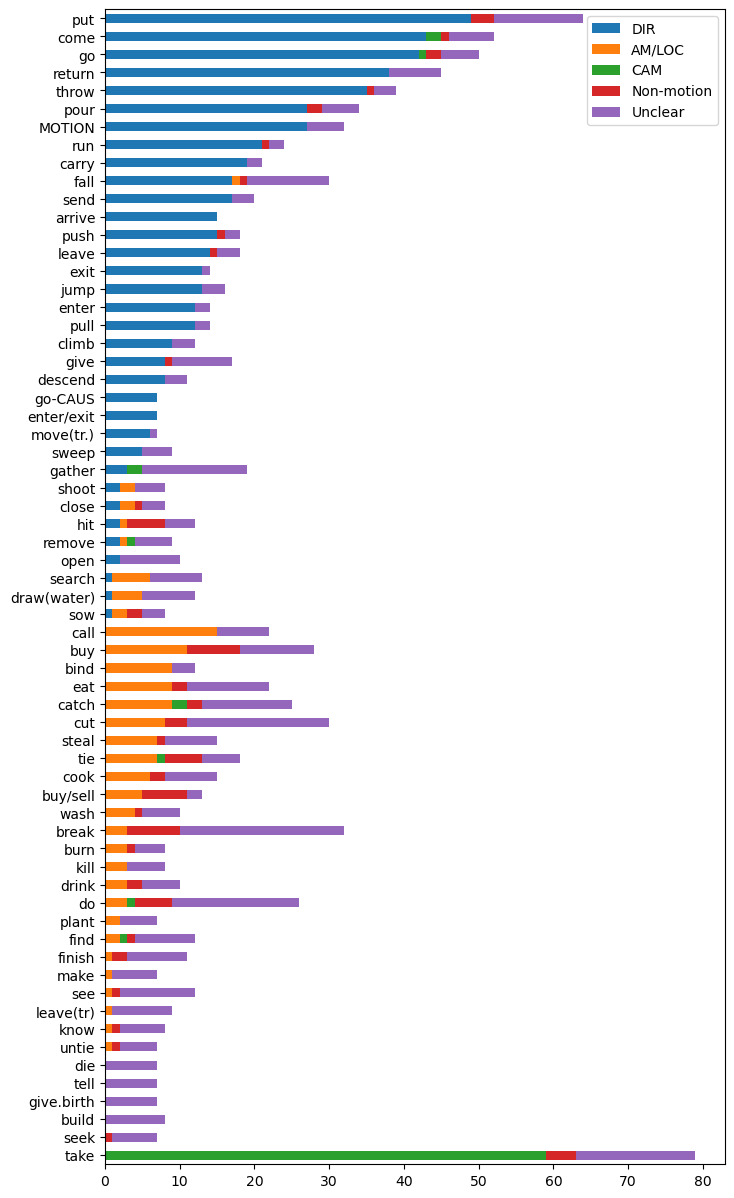
\includegraphics[width=0.85\textwidth]{figures/interpretation.png}
	\caption{Interpretations of extensions by verb gloss}
	\label{fig:interpretation}
\end{figure}

There are three general trends in how directional extensions tend to be interpreted when combined with a particular class of verb roots. First, directional extensions combined with prototypical motion verbs, unsurprisingly, nearly always result in a directional interpretation. However, there are a number of exceptions to this in the data. These are discussed in Section \ref{sec:interpretingmotion}. There is another group of verbs which are not typical motion verbs, but which can be given a directional reading in which some aspect of the event is construed as occurring along a literal path of motion. These verbs are discussed in Section \ref{sec:orientation}. They do not necessarily always have a directional interpretation, and are also commonly found with a subsequent motion interpretation. Finally, there are several verbs which are often presented as typical cases where a directional extension is given a subsequent motion interpretation. However, as discussed in Section \ref{sec:interpretingAM}, the same verb roots combined with directional extensions are also frequently found with non-motion interpretations. It cannot be assumed that the combination of a directional extensions with such verbs will always result in a subsequent motion interpretation.

\section{Motion verbs} \label{sec:interpretingmotion}

At the top of Table \ref{tab:interpretation1} and the top of Figure \ref{fig:interpretation} it can be seen that directional extensions most frequently have a directional interpretation when combined with prototypical verbs of motion such as `go', `return', `run' ,`jump', `exit' and `throw'. The high frequency of examples with a verb glossed `put' is possibly due to Chadic languages having several verbs for specific types of putting events which are all translated by English `put'. Directional extensions show a very strong bias toward a directional function when combined with motion verbs, but there are a number of exceptions. The exceptions are mostly idiomatic verb-extension combinations, as shown in (\ref{ex:mada0}), (\ref{ex:psik0}) and (\ref{ex:gude0}).  

\ea\label{ex:mada0}
\langinfo{\hyperref[mada]{Mada} verb \textit{pā} `put' with `side' suffix}{}{\cite[62]{ernstkurdiTenseAspectMood2016}} \\
\gll Ná-pā-fā-ŋ-và ma ...	\\
1\gl{sg}-put-\gl{side}-\gl{appl}-\gl{refl}.\gl{ipfv} \gl{top}	\\
\glt `I start...'

\ex\label{ex:psik0}
\langinfo{\hyperref[psik]{Psikye} verb \textit{dze} `go' with upward suffix}{}{\cite[117]{smithKapsikiLanguage1969}} \\
\gll nya malé dze-mé va cɛ	\\
\gl{dem} woman go-\gl{up} near house \\
\glt `This woman is standing near her house.'

\ex\label{ex:gude0}
\langinfo{\hyperref[gude]{Gude} verb \textit{hwa} `run' with ventive suffix}{}{\cite[203]{hoskinsonGrammarDictionaryGude1983}} \\
\gll hwa-ya	\\ 
run-\gl{vent}	\\ 
\glt `grow horizontally (of vine)'
\z 

Only in one case, shown in (\ref{ex:huba2}) above, is there a clear aspectual interpretation of a combination of a motion verb and directional extension. There is also only one example of a motion verb combining with a directional extension with an associated motion\index{associated motion} interpretation, rather than a directional interpretation. In (\ref{ex:pero4}), the \hyperref[pero]{Pero} verb \textit{cúg} `fall' combines with a ventive extension and is translated with a subsequent motion interpretation.\footnote{In the \hyperref[haus]{Hausa} data, there is also an example in which the verb \textit{sāw-ō} `put-\textsc{vent}' is translated as `put here, put on and come' \citep[662]{newmanHausaLanguageEncyclopedic2000}. The first translation is taken as a directional meaning when the verb has a transitive (caused) motion meaning. The second translation is taken as a separate meaning of the verb root which could be paraphrased as `dress'. In this case, the predicate is describing a non-motion event, and so the subsequent motion interpretation of the directional is as expected.} 

\ea\label{ex:pero4}
\langinfo{\hyperref[pero]{Pero} verb \textit{cúg} `fall' with ventive suffix}{}{\cite[94]{frajzyngierGrammarPero1989}} \\
\gll  cúg-ínà	tù	púccù \\
fall-\gl{compl}.\gl{vent}	\gl{prep} there	 \\
\glt `He fell there and subsequently came here.'
\z 

Finally, in \hyperref[glav]{Glavda}, the motion verbs \textit{s} `come' and \textit{d} `go' can combine with directional extensions to express caused accompanied motion. However, it should be noted that this meaning only arises with the transitive directional extensions which are distinguished from other extensions by beginning with \textit{d} (Chapter \ref{ch:identifying2}, Section \ref{sec:allomorphy}). Compare (\ref{ex:glav01}), where the verb \textit{s} `come' combines with the regular downward suffix and has a directional interpretation, with (\ref{ex:glav02}), where the same verb is combined with the transitive downward suffix and has a caused accompanied motion interpretation (`bring'), as further discussed in Chapter \ref{ch:CAM}. 

\ea\label{ex:glav01}
\langinfo{\hyperref[glav]{Glavda} verb \textit{s-} `come' with downward suffix}{}{\cite[]{owensGlavdaRuralUrban2011}} \\
\gll sə-xi	\\
come-\gl{down} \\
\glt `come down'

\ex\label{ex:glav02}
\langinfo{\hyperref[glav]{Glavda} verb \textit{s-} `come' with transitive downward suffix}{}{\cite[]{owensGlavdaRuralUrban2011}} \\
\gll sə-dií	\\
come-\gl{down}.\gl{tr}		\\
\glt `bring down'
\z 

\section{Orientation of an event} \label{sec:orientation}

There are a number of verb roots that are not typical motion verbs, but which can have a directional interpretation where the event they describe is construed as occurring along a path of motion. These include `shoot', `close', `remove', `hit', `open', `search', `draw (water)' and `sow'. Alternatively, these verbs can combine with a directional extension which is interpreted as a subsequent motion following the main event. 

For example, in (\ref{ex:haus02}), a \hyperref[haus]{Hausa} verb root glossed `shoot' is combined with a ventive marker and the interpretation is that the event takes place along a ventive path of motion, specifically that the projectile moves along a path of motion toward the speaker. Note that the existence of this projectile is entailed by the meaning of the verb, but it is not necessarily an argument of the verb. In (\ref{ex:bole0}), a \hyperref[bole]{Bole} verb root glossed `shoot' is combined with a ventive marker, but here the interpretation is subsequent ventive motion (or no translocative motion at all), rather than a directional interpretation.

\ea\label{ex:haus02}
\langinfo{\hyperref[haus]{Hausa} verb \textit{har̃b} `shoot' with ventive extension}{}{\cite[662]{newmanHausaLanguageEncyclopedic2000}} \\
\gll bā sā̀ har̃b-ô-wā	\\
?? ?? shoot-\gl{vent}-\gl{nmlz} \\
\glt `They are not shooting (at it) in this direction.'

\ex\label{ex:bole0}
\langinfo{\hyperref[bole]{Bole} verb \textit{màt} `shoot' with ventive extension}{}{\cite[39]{schuhBoleTangaleLanguagesBauchi1978}} \\
\gll mù màt-ín-kò	\\
1\gl{pl} shoot-\gl{vent}-\gl{pfv} \\
\glt `We shot (and brought).' or simply `We shot.'		
\z 

As another example, compare (\ref{ex:ngiz0}) and (\ref{ex:gude03}). In (\ref{ex:ngiz0}), a \hyperref[ngiz]{Ngizim} verb root glossed `close' is combined with a ventive extension with a directional interpretation. The path of motion that the door moves along is toward the deictic center. In (\ref{ex:gude03}), a \hyperref[gude]{Gude} verb root glossed `close' is combined with a ventive extension and the interpretation is subsequent ventive motion, rather than directional. 

\ea\label{ex:ngiz0}
\langinfo{\hyperref[ngiz]{Ngizim} verb \textit{cim} `close' with ventive extension}{}{\cite[81]{schuhAspectsNgizimSyntax1972}} \\
\gll miya mavgi da-cim-ayi	\\
mouth door \textsc{stative}-close-\gl{vent}		\\
\glt `The door is closed (this way).'

\ex\label{ex:gude03}
\langinfo{\hyperref[gude]{Gude} verb \textit{pya'} `close' with ventive extension}{}{\cite[98]{hoskinsonGrammarDictionaryGude1983}} \\
\gll  pya'-a	\\
close-\gl{vent}	\\
\glt `close and come'	
\z 

In data from \hyperref[bana]{Bana}, the verb root \textit{pla} `search' combined with a ventive extension can have either a directional or a subsequent motion interpretation. In (\ref{ex:bana0}), the interpretation is directional, while in (\ref{ex:bana01}), the interpretation is subsequent motion. 

\ea\label{ex:bana0}
\langinfo{\hyperref[bana]{Bana} verb \textit{pla} `search' with ventive extension}{}{\cite[44]{zuchGrammaireExercicesLangue1977}} \\
\gll  pla-ke vlé	\\
seek-\gl{vent} rabbit	\\
\glt `Go after the rabbit (in our direction)!' \newline
[French: `\textit{Chasse le lapin} (\textit{dans notre direction}) !']

\ex\label{ex:bana01}
\langinfo{\hyperref[bana]{Bana} verb \textit{pla} `search' with ventive extension}{}{\cite[44]{zuchGrammaireExercicesLangue1977}} \\
\gll pla-ke zer̂we!	\\
seek-\gl{vent} child	\\
\glt `Go look for the child (and bring him toward me)!' \newline 
[French: `\textit{Va chercher l'enfant} (\textit{et amène-le vers moi}) !']
\z 

The Bara examples in (\ref{ex:bana0}) and (\ref{ex:bana01}) are particularly interesting because both examples are of the same verb root from the same language, yet with two different interpretations of the directional extension. \citet[184]{belkadiDeicticDirectionalityAssociated2021} observes that ``motion and directional or path interpretations appear to be in complementary distributions across single languages.'' In other words, in most cases the available evidence allows an assumption that speakers of a particular language tend to be consistent in whether they allow a directional interpretation or an associated motion interpretation of a particular verb root -- even if there is variation across languages in regard to which verb roots fall into which category. As the Bara examples are the only counterexample in the dataset, \citet[184]{belkadiDeicticDirectionalityAssociated2021} appears to be correct that it is ``extremely rare for a form to be ambiguous between a directional interpretation and an additional motion event interpretation with a single verb [in a single language].'' However, it it also very possible that with more research on this topic, more counterexamples will be discovered.

\section{Subsequent motion and non-motion interpretations} \label{sec:interpretingAM}

Among those cases where a directional extension combines with a non-motion verb, one attested result is for the directional extension to receive a motion interpretation (other than directional) such as subsequent motion (Chapter \ref{ch:functions}, Section \ref{sec:comotion}). This interpretation is extremely common with verb roots that have glosses like `call', `buy', `bind', `eat', `catch', `cut' and `steal'. However, it is not the case that directional extensions always have a subsequent motion interpretation when combined with a non-motion verb. There are several non-motion verb roots that occur (cross-linguistically) with a directional extension that is given a non-motion interpretation. In other words, there is not a simple dichotomy between direction and associated motion in the interpretation of directional extensions across Chadic languages. 

A common case of non-motion interpretations of directional extensions is the idiomatic interpretation of specific verb-extension combinations. The most commonly found idiomatic use of directional extensions is the case of verbs glossed `buy' or `buy/sell'. In these cases, directional extensions take on the function of distinguishing between buying and selling events (Chapter \ref{ch:buysell}). In languages where this has not occurred, directional extensions tend to have a subsequent motion interpretation with a `buy' verb. 

Aspectual functions can also create a situation in which non-motion interpretations appear rather than subsequent motion interpretations. For example, in (\ref{ex:dghw01}) from \hyperref[dghw]{Dghwede}, the outward extension combined with the verb `cook' has a subsequent motion interpretation. In contrast, in \hyperref[bura]{Bura} the outward extension allows a aspectual interpretation, as shown in (\ref{ex:bura04}) where it combines with a verb glossed `cook'. 

\ea\label{ex:dghw01}
\langinfo{\hyperref[dghw]{Dghwede} verb \textit{tə́gə̀} `cook' with ventive outward extension}{}{\cite[6]{frickVerbalSystemDghwede1978}} \\
\gll kâ' tə́gə̀-díle kfì	\\
\gl{narr} cook-\gl{vent}.\gl{out} food		\\
\glt `She cooked food and brought it out.'

\ex\label{ex:bura04}
\langinfo{\hyperref[bura]{Bura} verb \textit{bwa} `cook' with outward extension}{}{\cite[4]{blenchBuraVerbalExtensions2010}} \\
\gll bwa-ɓəla	\\
cook-\gl{out}	\\
\glt `to cook thoroughly'
\z 

In \hyperref[bole]{Bole}, the ventive extension has a number of possible interpretations. In addition to a directional function, it can have a subsequent motion interpretation, a locative interpretation, a beneficiary interpretation or an idiomatic interpretation. In (\ref{ex:bole01}), the ventive form of the verb `eat' has a subsequent motion interpretation. In contrast, in (\ref{ex:bole02}), the ventive form of the verb `eat' has a beneficiary interpretation. Note that in (\ref{ex:bole02}) the verb also has a pronominal suffix referencing the beneficiary. This is part of the context that suggests (or perhaps even requires) a benefactive interpretation of the ventive extension. 

\ea\label{ex:bole01}
\langinfo{\hyperref[bole]{Bole} verb \textit{tíish} `eat' with ventive extension}{}{\cite[146]{gimbaBoleVerbMorphology2000}} \\
\gll à tíish-àakí-d-dí	\\
?? eat-\gl{vent}-\gl{vent}-\gl{add}	\\
\glt `He eats with it and comes.'

\ex\label{ex:bole02}
\langinfo{\hyperref[bole]{Bole} verb \textit{tíish} `eat' with ventive extension}{}{\cite[142]{gimbaBoleVerbMorphology2000}} \\
\gll tí-n-ní-n-tì	\\
eat-\gl{vent}-3SG.M-\gl{vent}-\gl{compl}	\\
\glt `He has eaten for him here.'
\z 

\section{Predicting interpretation through verbal semantics}

\citet{belkadiAssociatedMotionConstructions2016,belkadiDeicticDirectionalityAssociated2021} proposes an implicational hierarchy of verbs by lexical semantic types, shown in (\ref{ex:hierarchy}). Where verbal morphology can co-express either directional meaning or associated motion\index{associated motion} (DIR/AM), the hypothesis is that DIR/AM morphemes are more likely to have a directional interpretation with the verbs higher (further left) on this hierarchy and, conversely, are more likely to have an associated motion interpretation with the verbs lower on the hierarchy. 

\ea \langinfo{\textbf{Hierarchy of verbs by semantic type}}{}{\cite[191]{belkadiDeicticDirectionalityAssociated2021}} \label{ex:hierarchy} \\
Path motion > Motion translational > Causative motion > Perception >  Activities not involving translational motion > States 
\z 

The aim of the hierarchy in (\ref{ex:hierarchy}) is to go beyond a binary division between motion events and non-motion events in predicting the interpretation of morphemes that co-express directionality and associated motion\index{associated motion}. Belkadi's ``Path motion'' category includes directional motion events encoded in verbs with meanings like `descend', `enter' and `arrive'. The ``Motion translational'' category includes manner-of-motion verbs like `run', `jump' or `swim' where the event described involves a figure moving from one location to another. 

Belkadi does not provide any quantitative results of her study of 20 African languages. The hypothesis can be applied to the data in Table \ref{tab:interpretation1} and Table \ref{tab:interpretation2} but with a null result. Looking at the interpretations of DIR/AM verbal extensions in this dataset, it can be seen that all motion verbs elicit directional interpretations. Only one ``Motion translational'' verb (`fall') and one ``Causative motion'' verb (`remove') are additionally attested with an associated motion meaning. The rarity of associated motion interpretations among motion verbs in the data means that it is not possible to establish a statistically significant difference between ``Path motion'', ``Motion translation'' and ``Causative motion'' verbs. 

Non-motion verb roots in this dataset are nearly all ``Activities not involving translational motion.'' There is only one ``Perception'' verb root and one ``States'' verb root. For this reason, it is not possible to establish whether one subtype of non-motion verb root is more likely to elicit a directional or associated motion interpretation of a DIR/AM morpheme based on this data from Chadic languages. The only significant distinction in this dataset is a dichotomy between motion and non-motion verbs. 

\citet[368]{genettiDirectionAssociatedMotion2020} also tested Belkadi's hypothesis by applying a simplified version of Belkadi's hierarchy to data from 23 Tibeto-Burman languages. They provide quantitative data in regard to the first three types of motion verbs in (\ref{ex:hierarchy}). They conclude that ``although we must be tentative due to the small number of examples, overall the Tibeto-Burman data seem to confirm Belkadi’s proposed ranking'' \citep[371]{genettiDirectionAssociatedMotion2020}. However, there are a number of issues with that claim.

According to their coding of the data, DIR/AM morphemes are least likely to have an associated motion\index{associated motion} interpretation with manner-of-motion verbs. This interpretation is found in just 1 of 26 examples (4\%). DIR/AM morphemes have an associated motion interpretation when combined with directional (path-of-motion) verbs in seven of 65 examples (11\%). Causative motion verbs combined with DIR/AM morphology result in an associated motion interpretation in 11 of 53 examples (21\%).\footnote{\citet[370]{genettiDirectionAssociatedMotion2020} do not present the percentages as given here, but instead calculate what percentage of the 19 examples of associated motion interpretations with motion verbs are from each subclass, without regard to how many total examples there are of each subclass.} According to these statistics, DIR/AM morphology is least likely to have an associated motion interpretation when combined with manner-of-motion verb roots, and, therefore, manner-of-motion verbs should actually be highest on the hierarchy ahead of directional (path-of-motion) verbs. Causative motion verbs (or transitive motion verbs) most commonly result in an associated motion interpretation of DIR/AM morphemes, and are therefore the lowest of three motion types on the hierarchy, as predicted.

Furthermore, there are three issues with the coding of data in \citet{genettiDirectionAssociatedMotion2020}. First, several activity verbs are questionably classified as (translocative) motion verbs, including verbs glossed `hunt', `plough' and `search'. Second, several instances of directional meaning are classified as concurrent associated motion\index{associated motion}. In a footnote, \citet[370]{genettiDirectionAssociatedMotion2020} acknowledge that Antoine Guillaume made them aware of this issue, but they appeal to the ``exact translation'' as the basis of their classification. Having examined the relevant examples, it appears that the distinction between directional and associated motion was made on the basis of the syntactic structure of the English translation, rather than whether the event predicated by the verb is a translocative motion event \citep[as defined by][]{guillaumeAssociatedMotionSouth2016}. Third, they include examples translated as `leave behind' as associated motion, even though the examples do not necessarily make it clear that the relevant verbal morphology predicates a motion event (although it may be implied). In summary, upon closer scrutiny, \citet{genettiDirectionAssociatedMotion2020} do not have sufficient evidence to support the idea that motion verbs can be subcategorized semantically as to whether a co-expressive DIR/AM verbal morpheme is more likely to have an associated motion or directional interpretation. 



\section{Conclusion}

The data presented in this chapter on Chadic languages support the general notion that if a co-expressive verbal morpheme can express directional meaning, it will nearly always do so when modifying a motion verb. Most exceptions involve aspectual or idiomatic interpretations. Only very rarely does an associated motion interpretation appear with a motion verb. However, the data do not support Belkadi's \citeyear{belkadiAssociatedMotionConstructions2016} proposed fine-grained universal hierarchy of semantic types of verb roots in regard to interpreting co-expressive directional morphology. 

The data from Chadic languages also highlight the diversity of possible functions other than associated motion which may be co-expressed with directional meaning. The same morphemes that co-express direction and associated motion might also co-express a third function, as discussed in Section \ref{sec:interpretingAM}. There are 26 morphemes which, in addition to expressing direction, co-express associated motion as well as at least one other non-motion function, as in the \hyperref[bole]{Bole} examples in (\ref{ex:bole01}) and (\ref{ex:bole02}) above. This complexity cannot be captured in a simple dichotomy: if motion, direction; if not, associated motion. At this point, very little is known about how speakers interpret such multi-functional morphemes. There appears to be a considerable amount variation.

The other area of complexity is that there are events which involve some type of movement that is not linguistically structured as a translocative motion event (in the sense that none of the verb's arguments are a figure on a path of motion), but which can be construed as translocative motion when a directional extension is used, as discussed in Section \ref{sec:orientation}. Speakers have considerable flexibility to either construe the event as a motion event and interpret the verbal extension as directional, or to treat the verb root as non-motion and give another interpretation to the verbal extension such as subsequent motion. 

On the one hand, there is a very clear pattern in the grammar of Chadic languages allowing a great deal of certainty in predicting how directional extensions will be interpreted when used with a motion verb. On the other hand, there is a great deal of complexity in how directional extensions are interpreted when not used with a motion verb. The complexity involved in the interpretation of co-expressive verbal extensions does not lend itself to a straightforward compositional semantic analysis and requires a richer view of how speakers compose and interpret meaning. Verbal semantics alone are not always sufficient for predicting the interpretation of co-expressive directional extensions. Whether from language to language, or within a particular language, the interpretation of directional extensions depends not only on the lexical semantics of the verb, but on other factors, including grammatical context (such as other verbal morphology) and real-world context.

\chapter{Directed caused accompanied motion} \label{ch:CAM}

%is cam.verb-DIR much more common that I recorded? go through all 70 languages to check data? 

%Dryer 136
%It is not always clear, however, whether a morpheme is adding a separate motion
%event. One situation where there can be uncertainty is cases where a verb is glossed
%with something like `carry, take, bring'. Consider (16) from Huasteca Nahuatl.
%In (16), a ventive suffix (glossed `come') combines with a verb glossed as `bring'.
%One possibility is that the ventive suffix here is simply a directional, coding the
%direction of the bringing. The English verb bring is inherently ventive, but there
%are other Huasteca Nahuatl examples cited by Beller and Beller (1979) with the
%same verb walika that occurs in (16) but which Beller and Beller gloss as `take', so
%it could be that it is really the ventive suffix that yields the meaning `bring' rather
%than `take'.
%If the verb walika really does represent a motion event, then the ventive suffix
%in (16) is probably best viewed as a directional. However, a second possibility
%is that the event of bringing and the event of coming should be considered two
%separate motion events, in which case the ventive suffix in (16) is a marker of AM,
%not a directional. We must be careful, however, not to read too much into the
%way a verb is glossed. The English verbs carry, take, and bring all inherently code
%motion, but there may be cases where a verb that is glossed as `carry', `take' or
%`bring' can be used to include instances of holding, where there is no motion. If a
%ventive or andative morpheme combines with a verb of this sort, then it probably
%should be treated as a marker of AM rather than as a directional. In this chapter,
%I treat morphemes that combine with verbs glossed as `carry' or `take' as directionals rather than as markers of AM. However, some of these cases may turn
%out to be cases where the verb can mean something like `hold', in which case the
%morpheme should be treated as a marker of AM.

This chapter examines one functional domain in which some Chadic languages use directional extensions, namely, the expression of directed caused accompanied motion (e.g., `bring (here)', `take away'). By examining what means are used cross-linguistically to express a particular function, the use of directional extensions in this context is put into perspective as one morphosyntactic strategy among several that are found in various Chadic languages. 

\section{Expressing directed caused accompanied motion}

\citet{hellwigBringingTakingCrosslinguistic2022} introduce the notion of caused accompanied motion (CAM) as a cover term for the study of linguistic descriptions of bringing and taking events.  They focus on CAM events that are described as happening in a particular direction: directed CAM. They analyze directed CAM events as including four components of meaning: (translocative) motion, causation, accompaniment and directedness. Directed CAM events are frequently expressed through specialized morphosyntactic means. Among the morphosyntactic means for expressing directed CAM, \citet{hellwigBringingTakingCrosslinguistic2022} include four that are commonly found in Chadic languages. 

First, all components of directed CAM (including the directional component) may be expressed in a single verb root, as in the Barayin ventive CAM verb root \textit{sar} `bring' in (\ref{ex:bara0}), which contrasts with the Barayin itive CAM verb root \textit{kor} `take away'. This means for expressing directed CAM is discussed in \sectref{sec:dcamverb}.

\ea\label{ex:bara0}
\langinfo{\hyperref[bara]{Barayin} directed (ventive) CAM verb \textit{sar-} `bring' }{}{\cite[128]{lovestrandLinguisticStructureBarain2012}} \\
\gll kà sár-gì dō \\
3\gl{sg}.\gl{m}.\gl{sbj} bring-3\gl{sg}.\gl{m}.\gl{obj} \gl{neg} \\
\glt `He didn't bring it.'
\z

Second, a verb root which expresses general (non-directional) caused accompanied motion (e.g., `carry') may be modified by an additional element to express direction, as in the use of ventive directional morphology in (\ref{ex:kare8}). The use of this means for expressing directed CAM is discussed in \sectref{sec:modcamverb}.

\ea\label{ex:kare8}
\langinfo{\hyperref[kare]{Karekare} verb \textit{wula} `carry' with ventive suffix}{}{\cite[]{abareTCNN16Suleiman2016}} \\
\gll mendau yi 'wule-ne waɗa a mizitau \\
woman the carry-\gl{vent} food \gl{prep} male	\\
\glt `The woman brought food to her husband.'
\z 

Third, a directional motion verb may be modified to include the causation and accompaniment components of directed CAM meaning. This modification can be syntactic, as in the use of a comitative prepositional phrase in \hyperref[peve]{Pévé}, shown in (\ref{ex:peve7}), or it can be morphological, as in the use of a causative suffix in \hyperref[lama]{Lamang}, shown in (\ref{ex:lama09}). These means for expressing directed CAM are discussed in \sectref{sec:dirCAM}.

\ea\label{ex:peve7}
\langinfo{\hyperref[peve]{Pévé} directional verb with prepositional phrase}{}{\cite[217]{shayGrammarPeve2020}} \\
\gll ha mbə́ kə sə̀lày si su \\
2.\gl{m} come \gl{asoc} money \textsc{assertive} \gl{q} \\
\glt `Did you bring (lit. `come with') money?'

\ex\label{ex:lama09}
\langinfo{\hyperref[lama]{Lamang} directional verb with causative suffix}{}{\cite[142]{wolffLamangLanguageDictionary2015}} \\
\gll sá-ŋá-ghà \\
come-\gl{caus}-\gl{home} \\
\glt `bringing home'
\z 

Fourth, the use of a verb of acquisition (e.g., `take', `get') may be modified by a directional extension in order to express directed CAM, as in the ventive form of the verb \textit{hàw} ‘take' in \hyperref[kera]{Kera}, shown in (\ref{ex:kera06}). The use of this means for expressing directed CAM is discussed in \sectref{sec:takecam}.

\ea\label{ex:kera06}
\langinfo{\hyperref[kera]{Kera} verb \textit{hàw} ‘take' with ventive suffix}{}{\cite[116]{ebertSpracheUndTradition1979}} \\
\gll hàw-dà 	\\
take-\textsc{vent}	\\
\glt `Bring it here!'
\z 

\largerpage
To summarize, the four morphosyntactic means for expressing directed CAM that are examined for Chadic languages in this chapter are as follows:

\begin{enumerate} \itemsep0em 
	\item	Directed CAM verb root (e.g., `bring')
	\item	CAM verb root (e.g., `carry') + directional extension 
	\item	Directional verb root (e.g., `go', `come') + valency-increasing morphosyntax 
	\item	Verb of acquisition (e.g., `get', `take') + directional extension
\end{enumerate}

\tabref{tab:CAM} shows the number of languages (by branch) in which each of the four strategies for expressing directed CAM appear. For this study, a subset of 79 languages were included as the remaining languages were not considered to have sufficient information available to make any judgment on how directed CAM is expressed in the grammar. In 21 languages, more than one morphosyntactic means of expressing CAM are attested, so the totals  in \tabref{tab:CAM} show 100 means of expressing CAM across 79 languages. For nine of the 79 languages, no evidence of a morphosyntactic means of expressing directed CAM was found in the available data. The geographic distribution of these strategies for expressing directed CAM in Chadic languages is shown in \figref{fig:CAM}.

%data in tab:verbsbranch is from python code in file CAM 
\begin{table}
	\caption{Forms of directed CAM in Chadic languages (by branch)}
	\label{tab:CAM}
	\begin{tabularx}{\textwidth}{l Yrrr Y}
		\lsptoprule
{} &  West (21) &  Biu-M. (41) &  Masa (3) &  East (13) & Total \\
\midrule
Directed CAM verb     &     0 &            6 &     0 &     2 & 8 \\
Modified CAM verb &     4 &            9 &     0 &     0 & 13\\
Modified DIR verb   &    14 &           16 &     2 &     5 & 37 \\
Modified TAKE verb   &     6 &           25 &     1 &     1 & 32 \\
Not found     &     2 &            2 &     0 &     5 & 9 \\
\midrule
Total    &    26 &           58 &     3 &    13 & 100 \\
		\lspbottomrule
	\end{tabularx}
\end{table}

%see R code in file 'CAM map R code' 
\begin{sidewaysfigure}
	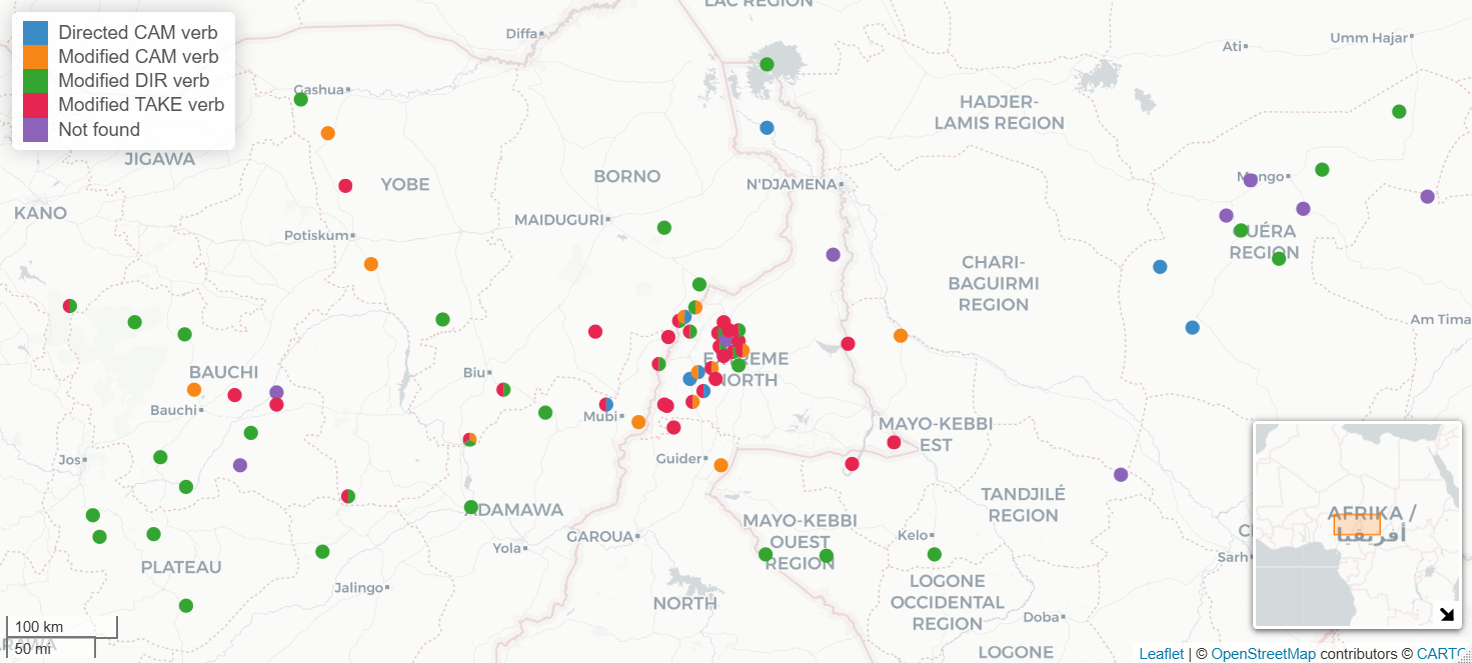
\includegraphics[width=\textwidth]{maps/CAM.png}
	\caption{Geographic distribution of forms for expressing directed CAM} \label{fig:CAM}
\end{sidewaysfigure}

\citet{hellwigBringingTakingCrosslinguistic2022} also discuss multiverb constructions used for the expression of directed CAM \citep[see also][104--106]{lovestrandSerialVerbConstructions2021a}. Multiverb constructions are not included in this study of Chadic languages due to the limited number of available descriptions. However, in those cases where grammatical descriptions do include multiverb constructions, no directed CAM functions are discussed.\footnote{Descriptions of multiverb constructions in Chadic languages include \citet[185--189]{shayGrammarPeve2020} on \hyperref[peve]{Pevé}, \citet[445]{frajzyngierGrammarGidar2008} on \hyperref[gida]{Gidar}, \citet[409]{allisonGrammarMakaryKotoko2020} on \hyperref[maka]{Makary Kotoko}, \citet[146]{wolffLamangLanguageDictionary2015} on \hyperref[lama]{Lamang}, \citet[210]{hoffmannGrammarMargiLanguage1963} on \hyperref[marg]{Margi}, \citet[269]{friesenGrammarMoloko2017} on \hyperref[molo]{Moloko}, \citet[215--218]{shayGrammarGizigaChadic2021} on \hyperref[gizi]{Giziga}, \citet[65]{viljoenGavarVerbPhrase2017} on \hyperref[gava]{Gavar}, \citet[2--3]{lienhardDabaGrammarClause1978} on \hyperref[daba]{Daba}, \citet[373--376]{frajzyngierGrammarMina2005} on \hyperref[mina]{Mina}, \citet[131--134]{thomasGrammarSakunSukur2014} on \hyperref[saku]{Sakun}, \citet[183--187]{frajzyngierGrammarLele2001} on \hyperref[lele]{Lele}, \citet[217]{peustSupplementsWestDangla2016} on \hyperref[dang]{Dangla}, \citet[250]{frajzyngierGrammarPero1989} on \hyperref[pero]{Pero}, \citet[412]{hellwigGrammarGoemai2011} on \hyperref[goem]{Goemai}, and \citet{lovestrandSerialVerbConstructions2018} on \hyperref[bara]{Barayin}. The most commonly reported function of multiverb constructions is the expression of prior motion, as is also commonly found cross-linguistically \citep{lovestrandSerialVerbConstructions2021a}.} This suggests that multiverb constructions are not a common syntactic structure used for expressing directed CAM in Chadic languages.

\section{Verb root expressing directed CAM} \label{sec:dcamverb}

The use of a directed CAM verb root is the least frequently attested means of expressing directed CAM, found in only eight languages.\footnote{These numbers potentially reflect under-reporting in the available data. Verb roots were only counted as lexicalization of directed CAM where the evidence made it clear that the verb stem could not be used as a general (non-directional) CAM verb (e.g., `carry') or as a verb of possession (e.g., `take'). General CAM verbs and verbs of possession are discussed separately as they often take on directed CAM meanings when modified by a directional extension.} In four of those languages, both a ventive and an itive CAM verb root are attested. In the other four languages, the only attested directed CAM verb root is ventive. The forms of directed CAM verb roots in the data are shown in \tabref{tab:dcamverbs}.

\begin{table}
	\caption{Forms of directed CAM verb roots} 
	\label{tab:dcamverbs}
	\begin{tabular}{llll} % add l for every additional column or remove as necessary
		\lsptoprule
		Language & Branch & VENT CAM & ITIVE CAM   \\ %table header
		\midrule
		\hyperref[dghw]{Dghwede} & Biu-Mandara & \textit{náxa} & \\
		\hyperref[maka]{Makary Kotoko} & Biu-Mandara & \textit{ɗō} &  \textit{do}  \\
		\hyperref[buwa]{Buwal} & Biu-Mandara & \textit{dā} & \textit{ɮāɗ} \\
		\hyperref[gava]{Gavar} & Biu-Mandara & \textit{daa} & \textit{dʒaɓ} \\
		\hyperref[mbud]{Mbudum} & Biu-Mandara & \textit{daha} & \\
		\hyperref[huba]{Huba} & Biu-Mandara & \textit{shìlnì} & \\
		\hyperref[bara]{Barayin} & East &  \textit{sèeró}, \textit{ajuro} & \textit{kóoro} \\
		\hyperref[soko]{Sokoro} & East & \textit{aaya} &  \\
		\lspbottomrule
	\end{tabular}
\end{table}

Three closely related Biu-Mandara languages, \hyperref[buwa]{Buwal}, \hyperref[gava]{Gavar} and \hyperref[mbud]{Mbudum}, show similar forms of verb roots for expressing directed CAM. There is likely an etymological link between the forms of these ventive CAM verbs and the ventive extension \textit{aha} which is still productive in these three languages. In \hyperref[bara]{Barayin}, there is a transparent etymological relationship between the directed CAM verb roots and the directional verb roots \textit{kóló} `go', \textit{ājó} `come' and \textit{síi} `come'. The stem-final \textit{-r} is probably from an erstwhile ``oblique'' suffix which likely had a valency increasing function \citep{robertsObliquesMawa2016}. 

In four of the seven languages with directed CAM verb roots, this strategy exists alongside another morphosyntactic means of expressing directed CAM. In \hyperref[buwa]{Buwal} and \hyperref[dghw]{Dghwede}, there is also evidence that general CAM verb roots can be modified by a directional extension to express directed CAM (\sectref{sec:modcamverb}). In \hyperref[mbud]{Mbudum} and \hyperref[huba]{Huba}, it is also possible to express directed CAM using a modified `take' verb (\sectref{sec:takecam}).

\section{Modified CAM verb} \label{sec:modcamverb}

In at least 13 languages, directed CAM may be expressed by a general CAM verb root (e.g., `carry', `transport') modified by a directional extension. For example, in \hyperref[bole]{Bole}, the general CAM verb root \textit{àlā} `carry, take from one place to another' has a ventive form \textit{èlen} `bring' \citep{gimbaBoleenglishhausaDictionaryAlhaji2004}. This may be an under-reported strategy, as many descriptions of languages with directional extensions only provide a limited number of examples. The absence of examples of CAM verbs modified by a directional extension may be a gap in the data. In regard to East Chadic languages, there are very few languages with directional extensions, so it is unsurprising that this strategy for expressing directed CAM is not reported in the East Chadic branch. 

In six languages, the use of a modified CAM verb appears to be the only morphosyntactic means of expressing directed CAM (in the available data). In the other seven languages, at least one of the other three strategies for expressing directed CAM are also attested. 

\section{Modified directional verb} \label{sec:dirCAM}

Nearly half of the languages in the sample, 37 of 79, can use a modified directional verb root (e.g., `come', `go') to express directed CAM. These can be divided into two categories. In 13 languages, the transported item is expressed in a prepositional phrase, as in (\ref{ex:nyam2}) and (\ref{ex:lele16}). In many languages, this preposition is identified as an associative preposition, as in (\ref{ex:lele16}). Associative is a label used in Chadic languages for a comitative preposition that also conjoins noun phrases. 

\ea\label{ex:nyam2}
\langinfo{\hyperref[nyam]{Nyam} verb \textit{tò} `come' with comitative prepositional phrase}{}{\cite[127]{andreasGrammatischeBeschreibungNyam2012}} \\
\gll mùdùk tò-wá yà kɔ̀lɔ́ŋ \\
woman come-\textsc{perf} with food \\
\glt `The woman has brought food.'

\ex\label{ex:lele16}
\langinfo{\hyperref[lele]{Lele} verb \textit{èje} `come' with associative prepositional phrase}{}{\cite[203]{frajzyngierGrammarLele2001}} \\
\gll èje dí ná kama \\
come 3\gl{sg} \gl{asoc} water \\
\glt `He brought water.'
\z 

In the other 24 languages, the directional verb root is used transitively so that the object of the verb is the transported item in the directed CAM event. Where directed CAM is expressed through increasing the valency of a directional motion verb, this is often described as a function of causative morphology, as in (\ref{ex:budu3}) and (\ref{ex:lama9}). In (\ref{ex:lama9}) the verb is further modified by an upward directional. 

\ea\label{ex:budu3}
\langinfo{\hyperref[budu]{Buduma} verb \textit{wú} `come' with causative suffx}{}{\cite[61]{lukasSpracheBudumaIm1939}} \\
\gll u-wú-re̤ \\
1\gl{sg}-come-\gl{caus} \\
\glt `I bring.' [German: `\textit{Ich bringe.}']

\ex\label{ex:lama9}
\langinfo{\hyperref[lama]{Lamang} verb \textit{s} ‘come’ with causative suffixes}{}{\cite[142]{wolffLamangLanguageDictionary2015}} \\
\gll
sá-ŋé-fé \\
come-\gl{caus}-\gl{up} \\
\glt `bringing up'
\z 

In other cases, verbal morphology with a similar function is described as marking transitivity rather than causation, as in the case of \hyperref[malg]{Malgwa} in (\ref{ex:malg13}). Alternatively, a valency-increasing suffix with a similar function may be described as an ``oblique'' marker \citep{robertsObliquesMawa2016}. Further comparative study would be needed to determine if there is any substantial variation in the functions of verbal morphology labeled `causative', `transitive' or `oblique'. 

\ea\label{ex:malg13}
\langinfo{\hyperref[malg]{Malgwa} verb \textit{d} `go' with transitive and outward suffixes}{}{\cite[139]{lohrSpracheMalgwaNara2002}} \\
\gll d-an-sé \\
go-\gl{tr}-\gl{out} \\
\glt `take away' [German: `\textit{wegnehmen}']
\z 

In at least two languages, \hyperref[mafa]{Mafa} and \hyperref[mbuk]{Mbuko}, directional verbs are labile and can be used in transitive contexts (expressing directed CAM) with no valency-increasing morphology on the verb, as in (\ref{ex:mbuk5}) where the noun phrase headed by \textit{zana} `cloth' is the direct object of the directional verb \textit{zla} `go'. 

\ea\label{ex:mbuk5}
\langinfo{\hyperref[mbuk]{Mbuko} verb \textit{zla} `go' as a transitive predicate}{}{\cite[22]{gravinaVerbPhraseMbuko2001}} \\
\gll Ta-zla anan zana a-tinen ahay pə-tila aga njavan ahay\\
3\gl{pl}.\gl{pfv}-go \gl{foc} cloth of-they \gl{pl} on-tailor house.of guinea-fowl \gl{pl}\\
\glt `They took their clothes from the tailor to the guinea-fowls’ house.'
\z 

\section{TAKE verb with a directional extension} \label{sec:takecam}

Besides modifying a directional verb, the other common strategy for expressing directed CAM is through the combination of a verb of possession (often glossed as `take') combined with a directional extension, as in (\ref{ex:haus7}) and (\ref{ex:mata12}).

\ea\label{ex:haus7}
\langinfo{\hyperref[haus]{Hausa} verb \textit{kāw} `take' with ventive extension}{}{\cite[663]{newmanHausaLanguageEncyclopedic2000}} \\
\gll kāw-ō \\
take-\gl{vent} \\
\glt `bring'

\ex\label{ex:mata12}
\langinfo{\hyperref[mata]{Matal} verb \textit{xə̀l} `take' with ventive extension}{}{\cite[294]{dougopheGrammarMatal2021}} \\
\gll  tá-xə̀l gwàʦàk àwáŋ áŋà  mà-ʦə̀ɗ-àj 	\\
3.\gl{pl}-take hen \gl{vent} \gl{purp} \gl{inf}-cut-??		\\
\glt `They bring a hen to slaughter...'
\z 

In languages with multiple directional extensions, it is possible for directionals other than ventive to be used to specify the direction of a CAM event, as in the use of the \hyperref[lama]{Lamang} downward suffix in (\ref{ex:lama12}). 

\ea\label{ex:lama12}
\langinfo{\hyperref[lama]{Lamang} verb \textit{ksa} ‘catch’ with downward extension}{}{\cite[78, 153]{wolffLamangLanguageDictionary2015}} \\
\gll ksa-gáa-tá	\\
catch-\gl{down}-\gl{compl}		\\
\glt `catching and taking downhill'
\z 

The strategy of modifying a `take' verb is particularly common among Biu-Mandara languages (25/41, 61\%). The higher frequency of the use of `take' verbs to express directed CAM in Biu-Mandara languages corresponds to the frequency at which directional extensions are found in each branch. However, this does not mean that all languages with directional extensions use a modified `take' verb for expressing directed CAM. Of the 79 languages in this sample, 54 have directional extensions. The modified `take' verb strategy is attested in 33 (61\%) of those languages.

\section{Conclusion}

Given the range of possible ways of expressing directed CAM, even among related languages, it is worth exploring the factors that may explain the distribution of various strategies for expressing directed CAM in Chadic languages. Two strategies are most commonly found: the use of a modified `take' verb root and the use of a modified directional verb root. The other two strategies are more rarely found: a directed CAM verb root and a modified CAM verb root. 

There is a pattern that correlates with the use of `take' verb roots in this context. As discussed in Chapter \ref{ch:functions}, directional extensions are typically multifunctional and one of the most common functions alongside direction is the expression of subsequent associated motion\index{associated motion}. Depending on the semantics of the event, it is possible for the subsequent motion to include a caused accompanied motion meaning, as in (\ref{ex:mafa3}).

\ea\label{ex:mafa3}
\langinfo{\hyperref[mafa]{Mafa} verb \textit{ta} `cook' with ventive suffix}{}{\cite[46]{barreteauLexiqueMafaLangue1990}} \\
\gll  n ta-ká mávə́r tə gáy	\\
3\gl{sg}.\gl{acc} cook-\gl{vent} boule in hut \\
\glt `She cooked the boule in the hut and brought it.' \newline
[French: `\textit{Elle a cuit la boule de mil dans la case et l'a apportée}.']
\z

%number in this paragraph from phyton code in CAM file
There are 34 languages with a directional extension that co-expresses subsequent associated motion\index{associated motion}. These include 32 of 33 languages which use the modified `take' verb strategy to express directed CAM.\footnote{The one exception is \hyperref[gizi]{Giziga} where most examples with non-motion verbs do not provide any indications of the function of the ventive directional suffix.} Since the use of `take' verbs for directed CAM is correlated with the subset of languages in which directional extensions co-express subsequent motion, it can reasonably be stated that (for Chadic languages) the use of `take' verbs to express directed CAM is a natural extension of the subsequent motion interpretation of directional extensions. This explains why not all Chadic languages with directional extensions use this strategy. Not all Chadic languages co-express subsequent motion meaning with a directional extension. 

This pattern indicates that (in Chadic languages) the motion component of the CAM expression is derived from the directional extension, not from the `take' verb root. By this account, there is no need to assume that the verb roots involved in these constructions have any inherent translocative motion meaning \citep[see discussion in][]{narasimhanPuttingTakingEvents2012}. If verb roots glossed `take' are assumed to be motion verbs, then it would be difficult to explain why many Chadic languages that have a directional extension do not use a modified `take' verb to express directed CAM. The explanation is that these Chadic languages have not developed the co-expression of subsequent motion that allows the use of `take' verbs to express directed CAM.

The use of valency-increasing morphosyntax with directional motion verbs is the other common strategy for expressing directed CAM, but its distribution is more difficult to account for. According to  \citet[][9]{jaggarHausaGrade52014}, the existence of causative forms of directional verbs expressing directed CAM can be taken as evidence that CAM expressions are semantically the causative counterpart of intransitive motion.\footnote{Contrast this view with \citet[31]{dixonTypologyCausativesForm2000} who assumes that a form in Yidiny which elsewhere has a causative function should be considered an applicative when used with a motion verb to express CAM.} From this point of view, there is nothing surprising about the presence of this strategy for expressing directed CAM. However, if this where a (universal) semantic structure, then it would be difficult to explain why it is not used in many languages where it is morphosyntactically possible. In addition, \citet[14]{hellwigBringingTakingCrosslinguistic2022} point out that, in the expression of CAM, other means of increasing the valency of intransitive motion verbs are just as common (or more common) than causativization. The use of causative forms in the expression of CAM is just one of several ways in which valency-increasing strategies may be repurposed to express a salient function. These appear to be idiomatic combinations that extend the meanings of productive morphology, and should not necessarily be subjected to synchronic semantic decomposition.  

We can also ask why the other two directed CAM strategies are relatively rare. Given the prevalence of directional morphology in Chadic languages, it might be expected that the combination of directional extensions with general CAM verb roots (e.g., `carry') would be a more commonly attested strategy for expressing directed CAM. As mentioned above, the apparent infrequency of this strategy may be an accidental gap in the data. However, another possible explanation is that some general CAM verb roots also specify the manner in which an item is transported. This additional semantic detail may fit the description of some types of directed CAM events, but it could make this strategy less ideal for the more general function of describing directed CAM without regard to manner. 

In regard to the rarity of verb roots that express all of the semantic components of directed CAM events (e.g., `bring'), there may be a more widespread cross-linguistic dispreference for maintaining directed CAM verb roots in the lexicon. In their sample of 13 languages from diverse language families, \citet[11]{hellwigBringingTakingCrosslinguistic2022} identify only two languages that express directed CAM as a verb stem. 

\chapter{BUY and SELL in Chadic languages} \label{ch:buysell}

Like the preceding chapter, this chapter focuses on a particular functional domain in which many Chadic languages employ directional extensions. Chapter \ref{ch:CAM} covers the domain of directed caused accompanied motion. This chapter covers the domain of commercial transactions, specifically buying and selling events. 

The ancestors of speakers of Chadic languages entered the Sahel region around 6,000 years ago \citep[71]{maceachernUnderstandingDistributionsChadic2018a}. They developed their languages in a context where commerce was predominantly done through trading goods. At some point in the last few millennia, the use of currency became the dominant mode of commerce. Speakers of Chadic languages began adapting to a new distinction: framing a commercial exchange in terms of which party gives or receives money (BUY or SELL).

Various strategies are used to make the distinction between buying and selling: the meaning of an existing verb may be extended, a verb may be borrowed from another language, or existing morphosyntactic forms can be co-opted to mark the distinction. The particular means used vary within each branch of Chadic languages in a way that does not align with genetic subgroupings. Yet, in this diversity, there is a remarkably consistent pattern of nearly always using an innovative form to overtly mark the SELL meaning, rather than BUY. This asymmetry reflects a goal-oriented bias in the expression of transfer of possession events \citep{lakustaStartingEndImportance2005,georgakopoulosFramingDifferenceSources2015}.

This chapter presents a study of the distribution of the various grammatical strategies that evolved for expressing these currency-related concepts in the grammars of 85 Chadic languages. Section \ref{sec:distinguishing} gives an overview of how many languages use each means of distinguish BUY and SELL. Cases of borrowed verbs or semantic shift to express SELL are discussed in Section \ref{sec:borrow}. Selling events can also be marked by verbal morphology (Section \ref{sec:SELLmorph}) or syntactic means (Section \ref{sec:SELLsyntax}). The rare instances of forms overtly marked for a BUY meaning are discussed in Section \ref{sec:BUYmorph}. Finally, Section \ref{sec:BUYsummary} provides a summary and discussion of the implications of this analysis.

\section{Distinguishing BUY and SELL} \label{sec:distinguishing}

Buying and selling events entail the exchange of money for goods. In a buying framing of the event (BUY), the person receiving the goods and giving money is the subject and the other participant is not necessarily a core argument, e.g., \textit{I bought a new car} (\textit{from my neighbor}). In a selling framing of the event (SELL), the person giving the goods and receiving the money is the subject and the buyer is not necessarily a core argument, e.g., \textit{I sold my car} (\textit{to my neighbor}). The distinction between BUY and SELL is an example that has been used by several linguists to illustrate how the same real world event can be construed differently by linguistic structures. \citet[25--26]{fillmoreTopicsLexicalSemantics1977} uses BUY and SELL to illustrate how different verbs can provide alternative ``perspectives'' on the same ``scene''.  \citet[77]{talmyCognitiveSemantics2000} refers to the choice between BUY and SELL as ``mapping of attention''. \citet[81]{geeraerts2000salience} refers to it as ``variational salience''. 

Many Chadic languages have a verb root that is ambivalent; it can be used for either BUY or SELL framing of a commercial transaction. For example, in \hyperref[dang]{Dangla}, the verb root \textit{gídy} (glossed `trade' in the original) occurs in the context of describing both BUY events (the subject is the buyer), as in (\ref{ex:dang0}), as well as SELL events, (the subject is the seller), as in (\ref{ex:dang1}). 

\ea\label{ex:dang0}
\langinfo{\hyperref[dang]{Dangla} verb \textit{gídy} `buy/sell' translated as BUY}{}{\cite[140]{shayGrammarEastDangla1999}} \\
\gll ŋu gidiy bèrka \\
3\gl{pl} buy/sell.\gl{pst} cow \\
\glt `They bought a cow.'

\ex\label{ex:dang1}
\langinfo{\hyperref[dang]{Dangla} verb \textit{gídy} `buy/sell' translated as SELL}{}{\cite[146]{shayGrammarEastDangla1999}} \\
\gll ŋa gidày-tʸa bèrka súgín-írá \\
3\gl{m} buy/sell.\gl{pst}-3\gl{f}.\gl{obj} cow market-\gl{loc} \\
\glt `He sold the cow at the market.'
\z

The label TRADE (in all capital letters) is used here for an unmodified verb root that can be used to express either BUY or SELL. In Dangla, the available data does not reveal any lexicalized or morphosyntactic mechanism for distinguishing BUY and SELL. This is the case for nine of the 85 Chadic languages in the sample. It may be that speakers rarely find themselves describing a context where there is ambiguity about the buyer and seller roles in a transaction, or such contexts may be so rare that non-grammaticalized means can be used, such as adding another phrase or clause to explicitly state who gave money and who received money in the transaction. It should be noted, however, there is limited documentation available for these nine languages, and so there is a strong possibility of a gap in the data.  

More commonly, languages with a TRADE verb root have a mechanism for distinguishing BUY and SELL. For example, the TRADE verb root \textit{pá} `buy/sell' in \hyperref[psik]{Psikye} is found in examples where it is translated `buy', as in (\ref{ex:psik28}), and also where it is translated `sell', as in (\ref{ex:psik29}). However, with the bushward suffix, as in (\ref{ex:psik25}), the verb can only express SELL.

\ea\label{ex:psik28}
\langinfo{\hyperref[psik]{Psikye} verb \textit{pá} `buy/sell'}{}{\cite[65]{smithKapsikiLanguage1969}} \\
\gll pa Hunter nde-ke ɗá cɛɗɛ ka-pa xá	\\
then Hunter give-\gl{vent} me money \gl{ipfv}-buy/sell millet \\
\glt `Then Hunter gave me money to buy millet.'

\ex\label{ex:psik29}
\langinfo{\hyperref[psik]{Psikye} verb \textit{pá} `buy/sell'}{}{\cite[60]{smithKapsikiLanguage1969}} \\
\gll pa xɛ́ vi-yi kweté wundú ka-pá nda ka xɛ́ 	\\
then 3\gl{pl} ??-put certain person \gl{ipfv}-buy/sell for ?? 3\gl{pl} \\
\glt `Then they put a certain person to sell (it) for them.'
\z 

\ea\label{ex:psik25}
\langinfo{\hyperref[psik]{Psikye} bushward form of \textit{pá} `buy/sell'}{}{\cite[114]{smithKapsikiLanguage1969}} \\
\gll 'a 'ya ké-pá-mte marure kwélékwelé	\\
\textsc{active} 1\gl{sg} \gl{ptcp}-buy/sell-\gl{bush} rice much \\
\glt `I sold a lot of rice.'
\z 

In Chadic languages, there are variety of means for distinguishing between BUY and SELL. \tabref{tab:BUYSELL} gives an overview of the how many languages have evidence of each of the strategies for distinguishing BUY and SELL. As seen in (\ref{ex:psik25}), one common strategy is to co-opt existing verbal morphology to modify a TRADE verb and designate the modified form as SELL. This is found in 29 of the 85 languages in the sample. Within this strategy, there is variation in which grammatical means are used to distinguish the meanings. The other common strategy, attested in 38 languages, is to incorporate a new verb root to make the distinction, either through borrowing or semantic shift. In this approach, the innovative verb root expresses SELL, and the meaning of an erstwhile TRADE verb may be restricted to only mean BUY.

Less commonly found means of making the distinction between BUY and SELL include the use of syntactic constructions with an adverbial or prepositional phrase (found in eight languages), and, in just four languages, the use of morphology to overtly mark a BUY event.

\begin{table}[H]
	\caption{Number of Chadic languages using each means for distinguishing BUY and SELL}
	\label{tab:BUYSELL}
	\begin{tabular}{l@{}rrrrr} % add l for every additional column or remove as necessary
		\lsptoprule
	{}	      &  West (26) &  Biu-M. (41) &  Masa (4) &  East (14) &  Total \\
	\midrule
No distinction       &     6 &            0 &     0 &     3 &      9 \\
%TRADE verb           &     9 &           12 &     0 &     7 &     28 \\
%BUY verb             &    17 &           28 &     4 &     7 &     56 \\
SELL verb            &     9 &           22 &     1 &     6 &     38 \\
SELL via syntax     &     3 &            2 &     1 &     2 &      8 \\
SELL via morphology &     8 &           16 &     2 &     3 &     29 \\
BUY via morphology  &     0 &            4 &     0 &     0 &      4 \\
		\lspbottomrule
	\end{tabular}
\end{table}

The geographic distribution of languages using various strategies for expressing SELL or BUY are shown in Figure \ref{fig:buysell}. The lack of clear geographical patterns suggest that there has not been a significant amount of contact or areal influence on the means for distinguishing BUY and SELL.

%see R code in file 'CAM map R code' 
\begin{sidewaysfigure}
	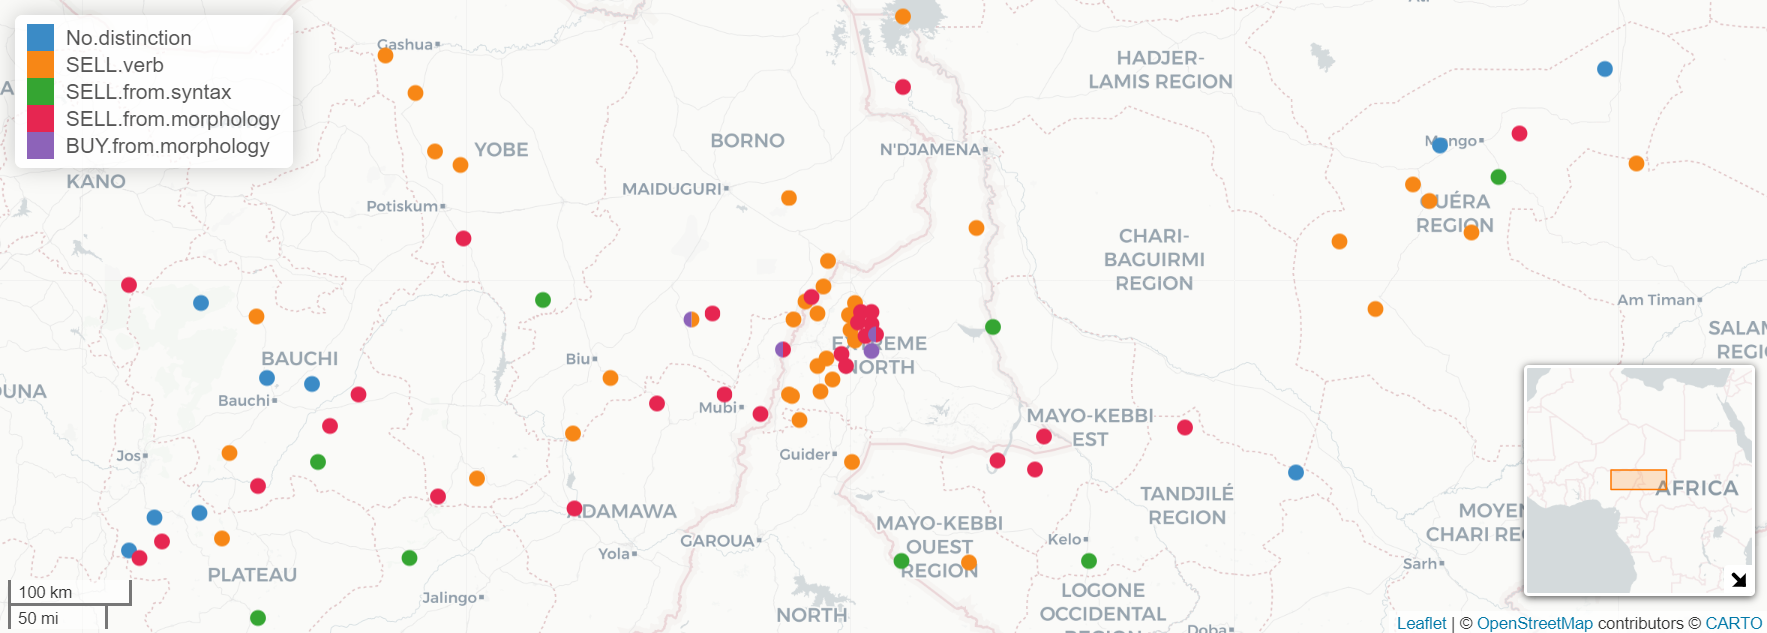
\includegraphics[width=\textwidth]{maps/buy-sell.png}
	\caption{Geographic distribution of forms for distinguishing BUY and SELL} \label{fig:buysell}
\end{sidewaysfigure}

\section{Borrowed verbs or semantic shift}  \label{sec:borrow}

Of the 85 Chadic languages in this sample, 57 have a verb root that expresses BUY. There are two reasons to assume that these BUY verb roots are erstwhile TRADE verb roots which have been restricted in their meaning.\footnote{The number of BUY verb roots may be over-reported relative to TRADE verbs. In multiple descriptions, a verb glossed as `buy' is found to actually be a TRADE verb which can also be used to express SELL. If this is a common oversimplification of how the lexical semantics of these verbs are documented, then it may be the case that more of the BUY verbs will turn out to actually be TRADE verbs.} The first reason is that TRADE and BUY verbs tend to be cognates. The clearest examples of cognates are from 20 Biu-Mandara languages where verb roots that have the consonantal structure \textit{*skm} or similar are frequently found to express TRADE or BUY, as shown in \tabref{tab:cognates}. Reflexes of this form are found in most Biu-Mandara subgroups including all six Dabaic languages, at least six Mofuic languages, six Mandaraic languages and both Hurza languages. Also shown in \tabref{tab:cognates} are likely cognates of the form \textit{*kl} expressing TRADE or BUY in four East Chadic A languages, and the form \textit{*st} for the same meanings in West Chadic A3 languages.  Other likely cognates for any verbs expressing TRADE, BUY or SELL are generally restricted to a single subgroup and only attested in two or three languages.\footnote{As discussed in Chapter \ref{ch:diachrony}, very few lexical items have been reliably reconstructed for Proto-Chadic.}

\begin{table}
	\caption{Verb root cognates expressing TRADE or BUY in Chadic languages}
	\label{tab:cognates}
	\begin{tabular}{llll}
		\lsptoprule
	Branch &	 Language 				&  TRADE &  BUY \\
		\midrule
Biu-Mandara & \hyperref[mbuk]{Mbuko} &   sukom &     \\
Biu-Mandara & \hyperref[vame]{Vamé} &  		  &    səm-  \\
Biu-Mandara & \hyperref[dghw]{Dghwede} &  	  &    skwá  \\
Biu-Mandara & \hyperref[park]{Parkwa} &  		  &    səkw  \\
Biu-Mandara & \hyperref[malg]{Malgwa} &  		  &    shə́kwa  \\
Biu-Mandara & \hyperref[zulg]{Zulgo-Gemzek} &    &    sékém  \\
Biu-Mandara & \hyperref[mada]{Mada} &  	skóm	  &      \\
Biu-Mandara & \hyperref[muya]{Muyang} &  	səkum	  &      \\
Biu-Mandara & \hyperref[wuzl]{Wuzlam} &  	sə̄kə̄m	  &      \\
Biu-Mandara & \hyperref[glav]{Glavda} &  	səgw	  &      \\
Biu-Mandara & \hyperref[molo]{Moloko} &  	skom	  &      \\
Biu-Mandara & \hyperref[mere]{Merey} &  			  &  səkəm    \\
Biu-Mandara & \hyperref[mata]{Matal} &  			  &  sə̀kw    \\
Biu-Mandara & \hyperref[buwa]{Buwal} &  	skām	  &     \\
Biu-Mandara & \hyperref[daba]{Daba} &  	səkəm	  &     \\
Biu-Mandara & \hyperref[gava]{Gavar} &  	 		  &  skəm   \\
Biu-Mandara & \hyperref[mafa]{Mafa} &  	 		  &  súm-   \\
Biu-Mandara & \hyperref[maza]{Mazagway} &  	 		  &  súm-   \\
Biu-Mandara & \hyperref[mbud]{Mbudum} &  	 		  &  sə̀kə̀m   \\
Biu-Mandara & \hyperref[mina]{Mina} &  	 		  &  skəm   \\
\midrule
East A & \hyperref[lele]{Lele} &  	kil 		  &     \\
East A & \hyperref[ndam]{Ndam} &  	kə́lə 		  &     \\
East A & \hyperref[somr]{Somrai} &  	 		  &    kələ  \\
East A & \hyperref[kwan]{Kwang} &  	 		  &    kèle  \\
\midrule
West A3 & \hyperref[mupu]{Mupun} &  	seet 		  &     \\
West A3 & \hyperref[ngas]{Ngas} &  	 		  &    síit  \\
West A3 & \hyperref[goem]{Goemai} &  s'éét	 		  &      \\
		\lspbottomrule
	\end{tabular}
\end{table}

The second reason to assume that BUY verb roots are erstwhile TRADE verb roots is that TRADE and BUY verb roots do not co-occur in the same language. As shown in \tabref{tab:TRADEV}, of the 56 languages with a BUY verb root, none of them have a TRADE verb root. This pattern is naturally explained if the development of BUY verb roots is a semantic restriction of verb roots that previously expressed TRADE.

%data in tab:TRADEV is from python code in file BUYSELL 
\begin{table}
	\caption{Number of languages with a TRADE, BUY or SELL verb roots}
	\label{tab:TRADEV}
	\begin{tabular}{rrrc}
		\lsptoprule
		{} & Has TRADE verb & No TRADE verb  & \% \\
		\midrule
		Has BUY verb 	 & 0 & 56  & \bwpie{0}{56} \\
		Has SELL verb & 6 & 32  & \bwpie{6}{32} \\
		\%  & \bwpie{0}{6} & \bwpie{56}{32} &  \\
		\lspbottomrule
	\end{tabular}
\end{table}

In contrast, as shown in \tabref{tab:TRADEV}, a SELL verb root co-occurs with a TRADE verb root in six languages. Unlike BUY verb roots which are frequently cognates with TRADE, there is just one likely cognate for TRADE and SELL. In the Bura-Marghi subgroup of Biu-Mandara,  we find \hyperref[marg]{Margi} \textit{ɗə̀l} TRADE and \hyperref[huba]{Huba} \textit{ɗəlá} BUY as well as \hyperref[bura]{Bura} \textit{dila} SELL and \hyperref[ciba]{Cibak} \textit{dəl} SELL.

Verb roots that express SELL are regularly described as expressing a range of meanings that include at least one meaning that possibly served as a historically prior meaning that was extended to express SELL. These can be divided into three groups: GIVE/SEND, THROW and LOSE. Four Mandaraic languages use a verb root \textit{vəl} to express SELL. There is evidence that this use is an extension of an older meaning related to transfer of possession. In \hyperref[glav]{Glavda}, the verb also means `give' and in \hyperref[wand]{Wandala} it also means `send'  \citep[155]{frajzyngierGrammarWandala2012}. In other languages, the verb for SELL also means `throw'. This is also the case for SELL verb roots \textit{daw} in \hyperref[mata]{Matal} and \textit{kal} in \hyperref[mere]{Merey}. The closely-related \hyperref[zulg]{Zulgo-Gemzek} verb \textit{kel} `sell' likely has the same history. Two East Chadic languages and one West Chadic language have verbs for SELL which also mean `lose' or `be lost'. This is true for \hyperref[bara]{Barayin} \textit{bito} `be lost' as well as \hyperref[mawa]{Mawa}. In \hyperref[tang]{Tangale} the notion SELL can  be expressed by the verbs \textit{sọgị} `spend, get rid of, lose, sell' and \textit{wayị} `let go, release, sell' \citep[146, 161]{jungraithmayrDictionaryTangaleLanguage1991}.\footnote{In \hyperref[lama]{Lamang}, the verbs \textit{skwa} ‘buy’ and \textit{dzawa} `sell' bear a resemblance to the verb roots \textit{skwa-} `come' and \textit{dza-} `go'. It is unclear whether this is a coincidence or evidence of a historical link.}

It is also possible that forms used to express SELL were borrowed from other languages. This is reported by some \hyperref[buwa]{Buwal} speakers for the verb \textit{bér} `sell' (Melanie Viljoen, personal communication), though it is not clear what the source language would be. This same form is used for SELL in all Dabaic languages. In the closely-related \hyperref[mafa]{Mafa} language, the verb for sell \textit{pə̀r-} `délier, vendre [untie, sell]’ is similar to the Buwal form, but its translation suggests that its use may be derived through a semantic shift. 

In summary, the comparative data provide evidence that verb forms that express TRADE or BUY are likely historical retentions, with BUY verb roots directly derived from erstwhile TRADE verb roots. In contrast, languages that have a verb root dedicated to expressing SELL have likely innovated this form through semantic extension or borrowing. 

\section{Verbal morphology distinguishing SELL}	 \label{sec:SELLmorph}

Besides innovating a new verb root for SELL, the second most common means of distinguishing SELL from TRADE or BUY is to use existing verbal morphology to derive a SELL verb from a TRADE/BUY verb root. This strategy is seen in 30 languages. In 12 of those languages, the morphology used to modify a TRADE/BUY verb root is used elsewhere as a valency-increasing device. In nine languages, the morphology used is used elsewhere as a directional extension. Finally, in nine other languages it is not clear what the function of the verbal morphology is outside of modifying a TRADE/BUY verb to mean SELL. This is either because of the limited data available or because the relevant morpheme is fossilized having lost any other function it previously had in the language. These fossilized forms will not be discussed in this section, as too little is currently known about their likely historical sources. 

\subsection{Valency-increasing morphology distinguishing SELL}	
\largerpage
Among the 12 languages that use a valency-increasing morphological alternation to mark SELL, the relevant morphological form is typically described as a causative. For example, in \hyperref[cuvo]{Cuvok}, the use of the ``causative'' suffix \textit{-dá} with the verb root \textit{husàm} `buy, sell' enforces the meaning `sell' \citep[315]{dadakGrammaireCuvokLangue2021}. This pattern raises the question of whether the concept SELL should be considered a semantically causative predicate (`cause to BUY'). The assumption that SELL is semantically causative is apparent in a description of \hyperref[paaa]{Pa'a} when \citet[189]{skinnerAspectsPaanciGrammar1979} states that, in regard to the verb \textit{kwan} `buy, sell', ``context determines meaning, no ± caus. difference''. Another example of assuming a causative semantic relationship between `buy' and `sell' is Schuh's proposed analysis of the \hyperref[ngam]{Ngamo} verb \textit{bò’ota} `sold' as the causative form of the verb \textit{kàja} `bought' despite the lack of any morphological evidence for this analysis \citep[332]{schuhChadicCornucopia2017}.\footnote{The same assumption is found in an analysis of German \textit{kaufen} `buy' and \textit{verkaufen} `sell'. The \textit{ver-} prefix is not productive and not used in causative contexts, yet \citet[270--271]{kastovskyCausatives1973} classifies the German example as an ``implicit causative''.} 

\largerpage
In \hyperref[haus]{Hausa}, the verb \textit{sàyaa} `buy' in a ``Grade 5'' form becomes \textit{sayar̃} `sell'.  \citet{jaggarHausaGrade52014} cites several scholars as authoritative sources that agree with his conclusion that SELL in Hausa is a semantic causative of BUY.\footnote{If we allow that the seller can be viewed as a causer, then it is equally plausible to view the buyer as a causer. This is precisely what \citet[191]{jackendoffSemanticStructures1990} proposes in giving Lexical Conceptual Structures for English \textit{buy} and \textit{sell} which differ only in which roles are linked to the argument of the outermost CAUSE function which instigates the event. Rather than analyzing \textit{sell} as the causative form of \textit{buy}, both verbs are seen as predicating caused events.} The only clear objection to this analysis is from \citet[398]{newmanEfferentialAliasCausative1983} who judges this analysis to be ``totally inaccurate and without justification.'' One of Newman's arguments is that within the Hausa language \textit{sayar̃} `sell' is not semantically equivalent to `cause to buy' which would be expressed by a periphrastic causative using the verb \textit{saà} `put, cause' \citep[402]{newmanEfferentialAliasCausative1983}.\footnote{The pattern in Hausa can be contrasted with Japhug (Sino-Tibetan) where \citet[17]{jacquesGrammarJaphug2021} uses the label ``inversive'' to refer to the use of a causative form to derive a SELL interpretation from the verb `buy': \textit{sɯ-χtɯ} [buy-\textsc{caus}]. However, this form is said to be translatable as either `cause to buy' or as `sell'.}

A cross-linguistic perspective on Chadic verbal morphology supports Newman's rejection of the analysis of SELL as a causative event. Morphemes that are labeled ``causative'' in Chadic languages often show patterns of use that do not map directly onto a semantic notion of causation as a relationship between a causal and caused event \citep{kulikovCausatives2001} or as the addition of a causer argument to a basic predicate \citep{dixonTypologyCausativesForm2000}. For example, in \hyperref[pero]{Pero}, the suffix \textit{-n} distinguishes \textit{pílù} `buy' from \textit{pílù-n} `sell'. The same suffix \textit{-n} is described as having a causative function in contexts like (\ref{ex:pero100}) where the agent-subject can be seen as causing the patient-object to act (`cause to eat'). 

\ea\label{ex:pero100}
\langinfo{\hyperref[pero]{Pero} verb \textit{cíyyó} `eat' with \textit{-n} suffix}{}{\cite[173]{frajzyngierGrammarPero1989}} \\
\gll cíyyó-n kà míjibà-ì \\
eat.\gl{pl}-\gl{caus} \gl{asoc} stranger-\gl{def} \\
\glt `Feed the strangers.'
\z 

The same \textit{-n} suffix also has a ``benefactive'' function in examples like (\ref{ex:pero101}). 

\ea\label{ex:pero101}
\langinfo{\hyperref[pero]{Pero} verb \textit{cíyyó} `eat' with \textit{-n} suffix}{}{\cite[173]{frajzyngierGrammarPero1989}} \\
\gll n-wálù-n ɓwé \\
and-cook-\gl{ben} gruel \\
\glt `...and the gruel was made for her.'
\z 

The general pattern within Chadic languages is that ``causative affixation is restricted to deriving transitive verbs from verbs that can only be used intransitively in their basic forms'' \citep[287]{schuhChadicCornucopia2017}. Rather than using the specific label \textit{causative} for such multi-functional forms, the more generic label \textit{valency-increasing} is more appropriate.\footnote{However, even this label does not capture all the uses of such morphology, as there is no difference in valency between BUY and SELL.} Given the fact that these valency-increasing morphemes are often found to express meanings other than causative, there is no compelling reason to assume that such morphemes are semantically or morphosyntactically causative in their function when they distinguish SELL from BUY. As \citet[175]{frajzyngierGrammarPero1989} notes in a comparison of Pero and Hausa, ``such an explanation would be purely ad hoc.''

The more likely explanation of why valency-increasing morphology comes to function as a means of distinguishing BUY and SELL stems from its applicative-like function as a marker of a beneficiary or other non-core argument. In the context of a transfer-of-possession event, such marking can refer to a recipient. Marking a non-subject recipient is incompatible with the BUY framing of a commercial transaction, and therefore must express a SELL framing. This underlying logic would explain why this form became conventionalized as a morphological means of making this distinction.\footnote{It remains to be seen whether this explanation has wider validity in other language families where forms labeled \textit{causative} distinguish SELL from BUY. A parallel case can be found in Puyuma (Formosoan) where a beneficiary suffix (glossed \textsc{cv}) is used to express the notion SELL: \textit{trima'-anay} `sell' [trade-\textsc{cv}]'. \citet[156]{kuoArgumentAlternationArgument2015} points out a similar pattern in Formosoan languages, but in those cases the suffix is labeled \textit{causative}: Amis, \textit{pa-qaca} `sell [\textsc{caus}-buy]' and Seediq, \textit{se-m-barig} `sell [\textsc{caus-av}-buy]'. \citet[387]{van1999generalized} mentions the German example alongside Lakhota \textit{ophéthų} `buy' and \textit{iyópheya} `sell' and Tagolog \textit{bili} `buy' and \textit{mag-bili} `sell'.}

Note, however, that not all Chadic languages with valency-increasing morphology use this strategy for distinguishing BUY and SELL. For example, in \hyperref[marg]{Margi} there is a valency-increasing (or causative) verbal suffix \textit{-ani}, but it is the itive directional extension that is used to distinguish SELL from TRADE \citep[119]{hoffmannGrammarMargiLanguage1963}.\footnote{Evidence from Kimaragang (Austronesian) provides further support for the notion that the combination of valency-increasing morphology and BUY verb roots only results in a SELL interpretation when this is lexically specified. There are two Kimaragang verbs for BUY: \textit{boli} and \textit{dagang} \citet[270]{kroegerCaseMarkingKimaragang1988}. While the ``two seem to be perfect synonyms'' the causative verb \textit{po-boli} means `cause to buy' and the causative verb \textit{pa-dagang} means `sell'. The most straightforward explanation of this pattern is that the form \textit{pa-dagang} `sell' is idiomatic.}  

\subsection{Directional extensions distinguishing SELL}	

Other than the valency-increasing (``causative'') forms used to distinguish SELL from TRADE or BUY, there are also at least nine languages that use directional extensions in the same way. Most of these languages use an itive directional extension to distinguish SELL from TRADE or BUY. For example, in \hyperref[wuzl]{Wuzlam}, the verb \textit{sə̄kə̄m} `\textit{acheter} [buy]' with the itive suffix becomes \textit{sə̄kə̄m-arə} `\textit{vendre} [sell]' \citep[162]{colombelLangueOuldemeNordCameroun2005}. In these cases the logic appears to be that the good exchanged is moving away from the seller toward a goal (the recipient).\footnote{The reason that the goods exchanged would be the moving object, and not the money exchanged, is that the exchange of money is lexically entailed and not expressed as a core argument. Therefore, it is the goods that are more likely to be seen as a figure on a path of motion.} \citet[134]{dryerAssociatedMotionDirectionals2021} notes the same pattern in Tamashek (Berber) and treats it as a directional since the ``metaphorical motion of what is bought or sold involves motion towards the buyer/seller or away from them.''

However, there are several reasons that BUY and SELL events should not be treated as motion events. It turns out that it is not always itive direction that is used to mark a SELL interpretation. Three languages use a different directional extension for this purpose. In \hyperref[gude]{Gude}, the verb \textit{ɗərə} `buy, trade' means `sell' when used with an upward/outward suffix: \textit{ɗərəgi} \citep[182]{hoskinsonGrammarDictionaryGude1983}. In \hyperref[psik]{Psikye}, it is the bushward suffix \textit{-mte}, as in (\ref{ex:psik25}).\footnote{The \textit{-mte} suffix in Psikye is also used for itive caused accompanied motion expressions with a `take' verb (Chapter \ref{ch:CAM}).} While the above can all generally be construed as depictions of SELL as an event moving away from a deictic center, the pattern in \hyperref[bole]{Bole} is the opposite. The verb \textit{gójju}  is translated `buy', and the ventive form of the verb, \textit{gòjùttù}, is translated `sell' \citep[36]{gimbaBoleenglishhausaDictionaryAlhaji2004}. As a West Chadic language, Bole has no directional extensions other than ventive. Nonetheless, this one exception demonstrates that there is nothing inherently itive or outward about the semantic relationship between SELL and BUY. A ventive directional extension can equally well distinguish the two concepts. 

Furthermore, if the combination of a BUY verb with itive direction was to be treated compositionally (BUY+ITIVE=SELL), some explanation would be needed for languages which have an itive directional extension and yet do not use it to distinguish BUY and SELL. Two languages, \hyperref[cuvo]{Cuvok} and \hyperref[dghw]{Dghwede}, have an itive extension and yet rather use a valency-increasing form to distinguish SELL. In addition, other directional extensions can be used to mark a BUY predicate. 

\section{Verbal morphology distinguishing BUY}	\label{sec:BUYmorph}

In four Biu-Mandara languages, there is a means of marking a verb meaning TRADE or SELL to instead mean BUY. In two of the languages, the directional extensions used align with the notion that BUY and SELL can be viewed as motion events in which the goods are moving away from or toward the subject. In Giziga, the verb \textit{hìɗík} can mean `trade, sell, buy', but in its ventive form, \textit{hìɗk-ò}, it explicitly means `buy' \citep[150]{shayGrammarGizigaChadic2021}. In \hyperref[molo]{Moloko}, a verb meaning TRADE marked with a ventive directional means BUY, as in (\ref{ex:molo13}). The same verb marked with an itive directional means SELL, as in (\ref{ex:molo14}). 

\ea\label{ex:molo13}
\langinfo{\hyperref[molo]{Moloko} verb \textit{skom} `buy/sell' with ventive marker }{}{\cite[240]{friesenGrammarMoloko2017}} \\
\gll nə̀-sʊkʷɔm=ala awak\\
1\gl{sg}.\gl{pfv}-buy/sell=\gl{vent} goat	\\
\glt `I bought a goat.'	

\ex\label{ex:molo14}
\langinfo{\hyperref[molo]{Moloko} verb \textit{skom} `buy/sell' with itive marker }{}{\cite[240]{friesenGrammarMoloko2017}} \\
\gll nə̀-sʊkʷɔm=alaj awak\\
1\gl{sg}.\gl{pfv}-buy/sell=\gl{itive} goat	\\
\glt `I sold my goat.'
\z

\hyperref[psik]{Psikye} is the one other language with morphological marking of both BUY and SELL meanings. As shown in (\ref{ex:psik25}) in Section \ref{sec:SELLmorph}, the SELL meaning appears with a rare bushward extension on a TRADE verb. The BUY meaning occurs when the same verb is marked with an outward extension, as in (\ref{ex:psik26}). This use of outward motion does not align with the view of BUY as describing goods moving toward the subject. 

\ea\label{ex:psik26}
\langinfo{\hyperref[psik]{Psikye} \textit{pá} `buy/sell' with outward extension}{}{\cite[114]{smithKapsikiLanguage1969}} \\
\gll  pá-ve ɗá wusú \\
buy/sell-\gl{out} 1\gl{sg} thing	\\
\glt `Buy me the thing!'
\z 

In \hyperref[ciba]{Cibak}, it is also the outward suffix that is used to mark a SELL verb root to express BUY, as in (\ref{ex:ciba4}). 

\ea\label{ex:ciba4}
\langinfo{\hyperref[ciba]{Cibak} verb \textit{də̀l} ‘sell’ with outward suffix}{}{\cite[133]{hoffmannZurSpracheCibak1955}} \\
\gll də́l-bà \\
sell-\gl{out} \\
\glt `buy' [German: `\textit{kaufen}']
\z 

In the use of verbal morphology to make a BUY-SELL distinction, there is a a clear asymmetry in the preferred marking of SELL rather than BUY, these four languages show that this is not without exception. Cibak is particularly exceptional in being the only language of the 85 in the data which does not have a verb root that can express BUY or TRADE on its own without a modifier. The data from these four languages also challenge the notion that BUY events are intrinsically linked with motion toward the deictic center. 

\section{Syntactic elements distinguishing SELL}  \label{sec:SELLsyntax}

In seven languages, the grammatical form that distinguishes a SELL interpretation from TRADE or BUY is said to be an independent element that is not part of the verbal morphology, although it is not always clear how consistently these criteria are applied cross-linguistically. In \hyperref[musg]{Musgu}, the adverbial \textit{àdí}, glossed as `\textit{en brousse, hors du village; vers l'extérieur} [in the bush, out of the village; toward the outside]' \citep[71]{tourneuxLexiquePratiqueMunjuk1991}, is used for this purpose. The adverbial is said to be the form that the itive verbal extension \textit{-di} is derived from \citep[133--134]{meyer-bahlburgStudienZurMorphologie1972}. In \hyperref[bidi]{Bidiya}, the adverb used for this function is \textit{ùnda} `\textit{devant} [in front of]' as in \textit{gìdày ùnda} `\textit{vendre} [sell]' \citep[78]{alioLexiqueBidiya1989}. In \hyperref[lele]{Lele}, it is also a bushward (and itive) adverbial that marks SELL events, as in (\ref{ex:lele12}). 

\ea\label{ex:lele12}
\langinfo{\hyperref[lele]{Lele} verb \textit{kil} `buy/sell' with itive adverbial \textit{cáaní}}{}{\cite[161]{frajzyngierGrammarLele2001}} \\
\gll kil	gé	kàmyá	tùmò	cáaní \\
buy/sell	3\gl{pl}	milk	before	to.bush/\gl{itive} \\
\glt `They used to sell milk.'
\z

In \hyperref[tera]{Tera}, the verb \textit{masa} `buy' combines with an itive particle \textit{masa ɓara} `sell' \citep[19]{newmanGrammarTeraTransformational1970}. Rather than grouping this form with the verbal morphology, \citet[314--315]{schuhChadicCornucopia2017} argues that it is better considered an adverbial, based on its syntactic distribution. In \hyperref[guru]{Guruntum}, the relevant form is said to be a preposition \textit{gʷǎi} `away'  \citep[173]{jaggarGuruntumGurdungWest1988}, but there is no further data showing its distribution. 

Causative forms are often described as a verbal suffix or postverbal particle, but in the case of \hyperref[peve]{Pévé} there is a periphrastic causative which is used to distinguish `sell' from `buy/trade', as in (\ref{ex:peve8}).

\ea\label{ex:peve8}
\langinfo{\hyperref[peve]{Pévé} multiword expression for `sell'}{}{\cite[59]{shayGrammarPeve2020}} \\
\gll  na ráʔ tímbì kunə kə́dàn gi tsoɓ rum(-u) \\
1\gl{sg} take calabash \gl{pl} \gl{purp} make purchase 3\gl{sg}(-\textsc{final.vowel}) \\
\glt `I took the calabashes in order to sell them.'
\z

There are also two West Chadic languages where the presence of a particular type of prepositional phrase used with a TRADE or BUY verb root signals a SELL interpretation. Parallel to the use of comitative phrases to express CAM (Chapter \ref{ch:CAM}, Section \ref{sec:dirCAM}), in \hyperref[nyam]{Nyam} a comitative prepositional phrase with the verb \textit{kemd-} `\textit{kaufen} [buy]' becomes `\textit{verkaufen} [sell]', as in (\ref{ex:nyam3}). \citet[127]{andreasGrammatischeBeschreibungNyam2012} describes this as a causative construction.

\ea\label{ex:nyam3}
\langinfo{\hyperref[nyam]{Nyam} verb \textit{kemd} `buy' with comitative prepositional phrase}{}{\cite[127]{andreasGrammatischeBeschreibungNyam2012}} \\
\gll mùdùk kémd-ì yà brédì \\
woman sell-\gl{hab} with bread \\
\glt `The woman usually sells bread.' [German: `\textit{Die Frau verkauft gewöhnlich Brot}.']
\z 

In \hyperref[goem]{Goemai}, the verb \textit{s'éét} `buy/sell' has a SELL interpretation when the item traded is expressed in a comitative prepositional phrase, as in (\ref{ex:goem2}).

\ea\label{ex:goem2}
\langinfo{\hyperref[goem]{Goemai} verb \textit{s'eet} `buy/sell' with comitative prepositional phrase}{}{\cite[217]{hellwigGrammarGoemai2011}} \\
\gll mòe=s'èèt m̠ép góe lá=kè \\
l\gl{pl}.\gl{sbj}=buy/sell(\gl{sg}) 3\gl{pl}.\gl{obj} with \gl{dem}.\gl{sg}.\gl{gen}=chicken \\
\glt `We sold them the little chicken.'
\z 

In these syntactic expressions we see the notions of movement away and causation (or increased valency) used to distinguish SELL from TRADE/BUY, as is commonly found where verbal morphology is used for the same function. There is a possibility that some of these examples are residue resulting from the lack of a clear method for distinguishing morphology and syntax. That ambiguity does not have a significant impact on the overall typology since it is only relevant for a small number of languages, and the semantic patterns of co-expression are similar to those found in verbal extensions. At least some of these cases, however, are quite clear examples of the use of syntactic constructions for this function. The semantic distinction between BUY and SELL can be made in verb roots, through verbal morphology or in a syntactic construction. 

\section{Conclusion}  \label{sec:BUYsummary}

The data from Chadic languages show that there are a variety of ways that languages may choose to distinguish SELL from BUY. A new verb root may be borrowed or the meaning of an existing verb root expressing transfer of possession (e.g., `give', `throw', `lose') may be extended to express SELL. There are two common morphological strategies used. One is to mark a SELL interpretation using valency-increasing morphology that evokes a non-subject recipient. The other is to use a motion metaphor of goods moving away from the subject to mark the SELL framing. These same strategies, valency-increasing and motion metaphor, are also seen in cases where syntactic constructions are employed to express SELL. 

Each of these strategies for expressing SELL are principled in their own right, but the choice of strategy is unpredictable from language to language, even within subgroups of closely related languages. \tabref{tab:SELLsemantics} shows, for each subbranch, how many languages use each of a particular semantic source for developing a means of distinguishing SELL from a TRADE or BUY verb root (including both morphological and syntactic constructions). This diversity confirms that these forms are recent innovations, not inherited from proto-forms.

\begin{table}[H]
	\caption{Number of Chadic languages using each type of semantic source to develop an overt marker for SELL events}
	\label{tab:SELLsemantics}
	\begin{tabular}{lrrrrr} % add l for every additional column or remove as necessary
		\lsptoprule
		Subbranch	      &  ITIVE/BUSH & VENT & OUT & Valency &  Other \\
		\midrule
West Chadic A	& 0 & 1 & 0 & 4 & 4 \\
West Chadic B	& 1 & 1 & 0 & 1 & 0 \\
Biu-Mandara Hurza & 0 & 0 & 0 & 2 & 0 \\
Biu-Mandara North & 2 & 0 & 2 & 3 & 1 \\
Biu-Mandara South & 2 & 0 & 1 & 2 & 0 \\
Masa			  & 0 & 0 & 0 & 1 & 2 \\
East Chadic A	& 1 & 0 & 0 & 2 & 2 \\
East Chadic B	& 0 & 0 & 0 & 1 & 1 \\
		\lspbottomrule
	\end{tabular}
\end{table}

The choice of strategy for distinguishing BUY and SELL cannot be predicted from morphosyntactic properties of each language. These expressions are best viewed as idiomatic expressions. While there are clear metaphorical principles that motivate the use of some forms more than others, the adoption of a particular strategy seems mostly arbitrary. Therefore, complex forms that distinguish BUY and SELL should not be incorporated into a decompositional semantic analysis.

Another pattern that emerges from these data is the striking asymmetry in the overt marking of forms to express SELL. There is substantial evidence of SELL verb roots being innovated, while BUY verb roots appear to be retentions of TRADE verb roots. Morphologically, it is nearly always the SELL form that is marked in comparison to a BUY or TRADE form. Only in four languages is there a BUY form that is overtly marked by verbal morphology, and, in three of those, the marked BUY form exists alongside a marked SELL form. Syntactically, it is also the case that overtly marked forms express SELL, and not BUY.

There are two possible explanations for this pattern. It may be that BUY is less marked (``zero coding'' vs ``overt coding'') because it is the more frequently used expression \citep[43--44]{haspelmathMarkednessWhatReplace2006}. In a cash economy, it is more common to discuss buying than selling. Even farmers or pastoralists who sell their goods would only periodically act as vendors, while they would act as consumers on a much more regular basis. In such a context, the more frequently used meaning may become the default interpretation. 

A second possible explanation for the markedness of SELL is that there is a cognitive bias towards expressing the ``goal'' or recipient argument of transfer of possession events \citep{lakustaStartingEndImportance2005,georgakopoulosFramingDifferenceSources2015}. The BUY interpretation expresses the recipient as subject, thereby matching the speakers' expectation. In contrast, SELL verbs do not express the recipient as a core argument, and so are marked to signal that they go against the default interpretation. 

This comparative study of BUY and SELL forms across Chadic languages provides insights into how to best analyze individual Chadic languages. Morphologically complex forms and syntactic constructions for distinguishing SELL from TRADE or BUY (and, in rare cases, for marking BUY) can be treated as idiosyncratic expressions that were relatively recently adopted. These exceptional forms are the linguistic traces of the socio-economic shift to currency as the dominate means of commercial transaction. 

\chapter{Summary and future directions} \label{ch:summary}

The goals of this book as outlined in the introductory chapter are to improve the state of description of the grammars of Chadic languages, contribute to the typology of Chadic and Afroasiatic languages, and to provide insights into the nature of how motion is expressed through linguistic structures.

\section{Chadic languages}

The concepts outlined in this book, especially the types of directional meaning (Chapter \ref{ch:distribution}) and the typology of co-expression with directional meaning (Chapter \ref{ch:functions}) provide a framework for describing and comparing this frequently attested element of Chadic verbal morphology. The use of consistent comparative concepts applied to each of the Chadic languages covered in this book have made their descriptions more cohesive and accessible, and the process also provided an occasion to review and correct some of the inconsistencies found in past publications (as detailed in the appendices). 

One improvement needed in future descriptive work is a more explicit and consistent analyses of the function of directional extensions with all kinds of verbs. Our understanding of how speakers of Chadic languages use directional extensions is significantly limited due to the fact that in half of the examples of directional extensions it is not clear what the function is (Chapter \ref{ch:functions}). It is possible that many of the translations that lack an explicit translation of the directional extension's function are cases of aspectual uses of directional extensions. This is a topic that deserves more attention in future descriptive work. Another area of particular interest for future description is to have more detailed descriptions of the few languages where different forms of directional extensions are used for intransitive and transitive predicates (Chapter \ref{ch:identifying2}, Section \ref{sec:allomorphy}). This type of morphology is attested in associated motion paradigms, but not frequently discussed in regard to directional extensions.

The quantitative results presented in Chapter \ref{ch:distribution} give a clear picture of the distribution of directional extensions in Chadic languages which provide a set of general expectations for anyone describing the verbal morphology of Chadic languages. Directional extensions are common, but not ubiquitous. Ventive directional extensions are widespread. Other types of directional extensions are mostly limited to Biu-Mandara. Most languages with directional extensions have only one or two types, usually ventive and itive. In the minority of languages with three or more types of directional extensions (all from Biu-Mandara), less common types, such as bushward and `onto' directions, are attested, while the more common ventive type may actually be absent. 

In the large-scale typological approach of Grambank \citep{thegrambankconsortiumGrambankV12023}, directional verbal morphology is addressed by the single binary question ``Is there directional or locative morphological marking on verbs?'' By comparison, this study of directional verbal morphology in Chadic language is fine-grained and considers variation in the semantic types of directional extensions and their multi-functionality. \citet{martenParametersMorphosyntacticVariation2007} use the term ``micro-variation'' to describe the study of morphosyntactic variation within the context of a family of languages with many shared morphosyntactic features. A statistical approach to micro-variation is what allows this study of directional extensions to affirm the classification of Biu-Mandara languages as a distinct branch. The sub-classification of Chadic languages relies primarily on comparing lexical items. 

Observations about classification naturally raise diachronic questions about how these differences came to be over time. As \citet[5]{schuhChadicCornucopia2017} observes, ``comparative Chadic studies are at an early stage... Aside from some broad areas of agreement, such as the genetic unity of West Chadic or the reconstructability of grammatical gender, there is no `received knowledge' that everyone agrees on.'' In the case of West Chadic languages, the patterns observed suggest that ventive directional extensions are an old type of directional extensions. This analysis is supported by the plausible reconstruction of ventive directional extensions for West Chadic languages (Chapter \ref{ch:diachrony}). However, the fact that ventive directional extensions cannot be reconstructed for Proto-Chadic leaves open the possibility that their frequent appearance could be due to areal influence and might not be a reliable indicator of genetic affiliation. This also applies to the parallels found in other Afroasiatic families, Berber and Semitic, where ventive forms are common \citep{belkadiAssociatedMotionDeictic2015,belkadiAssociatedMotionConstructions2016,fixSemanticsSemiticVentive2020}.

\section{Motion in grammar}

This book makes three main contributions to the study of motion in grammar. First, the comparison of verb roots and verbal morphology in Chapter \ref{ch:verbs} presents a new perspective on the verb-satellite distinction proposed by \citet{talmyLexicalizationPatternsSemantic1985}. It is demonstrated that within the verbal complex of Chadic languages a complementary distribution tendency can be identified such that certain directional meanings (boundary-crossing and vertical) are either found lexicalized in a verb root or grammaticalized in a verbal extension, but not both. This result provides insights into ways in which grammars can evolve to be more efficient and avoid redundancy. However, the same pattern does not hold for ventive and itive directional extensions. This suggests a fundamental distinction between ventive and itive and other types of directional meaning. This type of distinction would not be apparent in research that conflates all types of path of motion into one category. 

The second contribution to the study of motion in grammar is the analysis in Chapter \ref{ch:interpretation} of how co-expressive directional extensions are interpreted. Directional extensions in Chadic languages are multi-functional (Chapter \ref{ch:functions}). The most common function co-expressed with direction is subsequent associated motion. There are also cases of grammaticalized functions co-expressed with direction, and there are many lexicalized uses of combinations of a verb root and a directional extension. Generally speaking, directional extensions have a directional interpretation when used with predicates that describe motion events, with only a limited number of exceptions. Most of these exceptions are cases where a verbal extensions that expresses direction also co-expresses a grammaticalized non-motion meaning, such as aspect. When directional extensions are used with non-motion verbs, the patterns are much more complex -- even unpredictable. Previous studies have focused on the prevalence of associated motion\index{associated motion} interpretations in this context \citep{belkadiAssociatedMotionDeictic2015,belkadiAssociatedMotionConstructions2016,genettiDirectionAssociatedMotion2020,rossCrosslinguisticSurveyAssociated2021}. However, in Chadic languages, other interpretations are possible, especially aspectual meaning and lexicalized combinations.

Where more than one interpretation is possible, the lexical semantics of the verb root is not always sufficient for predicting the interpretation of the directional extension. This is due (in part) to the flexibility that speakers have to frame events with movement (e.g., shooting, closing) as translocative motion events with a moving figure that is not necessarily an argument of the verb. A straightforward analytical approach to composing the meanings of verbs and directional extensions cannot account for this feature of directional extensions without taking into account pragmatic factors \citep{nikitinaPragmaticFactorsVariation2008}. Across linguistic phyla the picture becomes even more complex. Whereas directional extensions in Chadic languages tend to co-express subsequent associated motion (except for those cases where a ventive directional expresses itive prior motion), directional morphology in other languages may tend to co-express prior motion, concurrent motion or some combination \citep{dryerAssociatedMotionDirectionals2021}. Other languages, like English, do not co-express associated motion with directional markers at all. The reasons for these various patterns are not immediately apparent.  

The third contribution to the study of motion in grammar is the correction of previous suggestions that verbs of acquisition (e.g., `take') should be analyzed as motion verbs (Chapter \ref{ch:CAM}) and that buying and selling can be analyzed as motion events (Chapter \ref{ch:buysell}). Since directional morphemes are used in these contexts in Chadic languages, it is not unreasonable to hypothesize that these verbs describe motion events. However, by looking at how these functions are expressed across Chadic languages, it can be seen that this is not a consistent cross-linguistic feature of Chadic languages. Rather, it is one way that these meanings have been lexicalized. Another common form used to lexicalize these meanings is a valency-increasing form, such as a causative. Likewise, treatments that suggest that the use of causative (or valency-increasing) forms in this context is an example of semantic causation are an over-analysis of the grammar. 

The final point to be made is that this book is designed with the assumption that it likely contains some omissions or errors. In case the need for any substantial changes to the data is discovered, the database has been archived in an online deposit in Zenodo \citep{lovestrandDirectionalsChadic2023} so that a new, updated version can be created. Since the same deposit includes the Python scripts used for the calculations, these can be redone in a straightforward manner. Likewise, the publisher, Language Science Press, was chosen for this book because of their online, open access approach to publishing which allows authors the opportunity to update their publications in new editions. Another reason for choosing an online publisher is that this permits the inclusion of an extended set of appendices. The appendices include an account of how the data for each language included in the study were interpreted, and to allow anyone with expertise in a particular Chadic language to offer constructive feedback to the author on any points that need improvement. 


\appendix
\renewcommand{\thesection}{\arabic{section}} 
\renewcommand{\thesubsection}{\thesection.\arabic{subsection}}
\chapter{West Chadic (29/84)}

West Chadic languages are divided into two subbranches. Descriptions are available for the grammar of 22 of the 46 West Chadic A languages. Descriptive coverage of the West Chadic B languages is much poorer with descriptions available for only seven of 38 languages. 

\section{West Chadic A (22/46)}

The 46 West Chadic A languages are divided into four groups. In each group, grammatical descriptions are available for half of the languages or more, with the exception of West Chadic A3. 

\subsection{West Chadic A1 (1/2)}

No description of the morphosyntax of Gwandara (gwan1268) is available, so only Hausa is included here.

\paragraph*{Hausa (haus1257)} \label{haus}

Information on Hausa grammar comes mainly from a reference grammar \citep{newmanHausaLanguageEncyclopedic2000}. 

\largerpage
\subparagraph{Directional verbs}~
~


\begin{table}[H]
	\caption{Hausa directional verbs} 
	\label{tab:hausV}
	\begin{tabular}{lll} % add l for every additional column or remove as necessary
		\lsptoprule
		DIR & verb & gloss   \\ %table header
		\midrule
		ITIVE & \textit{tafi} & `go' \\
		VENT & \textit{zo} & `come' \\
		UP & \textit{hawa} & `go up, climb' \\
		DOWN & \textit{sauka} & `descend' \\
		INTO& \textit{shiga} & `enter' \\
		OUT & \textit{fita} & `exit' \\
		\lspbottomrule
	\end{tabular}
\end{table}

\subparagraph{Directional extensions}~



\begin{table}[H]
	\caption{Hausa directional morphology}
	\label{tab:haus}
	\begin{tabular}{llll} % add l for every additional column or remove as necessary
		\lsptoprule
		forms & source gloss & directional  & other functions  \\ %table header
		\midrule
		\textit{-ō}  & Grade 6  &   \textsc{vent} &  \textsc{subs.vent, loc}  \\
		\lspbottomrule
	\end{tabular}
\end{table} 

The Hausa ventive suffix is a long vowel \textit{-ō} traditionally called ``Grade 6'' in the study of Hausa verbal morphology. ``The ventive ending generally denotes action or movement in the direction of the speaker (or any other pragmatically established deictic center)…'' \citep[663]{newmanHausaLanguageEncyclopedic2000}, as in (\ref{ex2:haus1}) and (\ref{ex2:haus2}).

\ea\label{ex2:haus1}
\langinfo{Hausa verb \textit{fit} `exit' with ventive suffix}{}{\cite[663]{newmanHausaLanguageEncyclopedic2000}} \\
\gll fit-ō \\
exit-\gl{vent} \\
\glt `come out'

\ex\label{ex2:haus2}
\langinfo{Hausa verb \textit{jany} `drag' with ventive suffix}{}{\cite[663]{newmanHausaLanguageEncyclopedic2000}} \\
\gll jany-ō \\
drag-\gl{vent} \\
\glt `drag in this direction'
\z 

The same suffix also ``sometimes indicates `do some action and come'{''} \citep[663]{newmanHausaLanguageEncyclopedic2000}, in other words, subsequent associated motion, as in (\ref{ex2:haus3}) and (\ref{ex2:haus4}). 

\ea\label{ex2:haus3}
\langinfo{Hausa verb \textit{shāf} `whitewash' with ventive suffix}{}{\cite[663]{newmanHausaLanguageEncyclopedic2000}} \\
\gll nā	shāf-ō	bangō	 \\
I	whitewash-\gl{vent}	wall \\
\glt `I whitewashed the wall and came back.'

\ex\label{ex2:haus4}
\langinfo{Hausa verb \textit{said} `sell' with ventive suffix}{}{\cite[664]{newmanHausaLanguageEncyclopedic2000}} \\
\gll said-ō \\ 
sell-\gl{vent} \\
\glt `sell and come back'
\z 

In one example, shown in (\ref{ex2:haus5}), the interpretation of the ventive suffix is subsequent caused accompanied motion.

\ea\label{ex2:haus5}
\langinfo{Hausa verb \textit{say} `buy' with ventive suffix}{}{\cite[663]{newmanHausaLanguageEncyclopedic2000}} \\
\gll yā	say-ō	nāmā̀ \\
he	buy-\gl{vent}	meat \\
\glt `He bought some meat and brought it back here.'
\z 

In at least one case, a verb with a ventive suffix can be interpreted as either directional or subsequent associated motion. In (\ref{ex2:haus6}), the verb `put' with a ventive suffix can either be directional in a transitive sense where the object is moving towards the deictic center, or as subsequent associated motion where the verb is interpreted (intransitively) as `getting dressed'. 

\ea\label{ex2:haus6}
\langinfo{Hausa verb \textit{sāw} `put' with ventive suffix}{}{\cite[662]{newmanHausaLanguageEncyclopedic2000}} \\
\gll sāw-ō \\
put-\gl{vent} \\
\glt `put here, put on and come'
\z 

The are also some uses of ventive forms that have no motion meaning including \textit{ɓull-ō} `appear suddenly' and \textit{far̃faɗ-ō} `revive' \citep[663]{newmanHausaLanguageEncyclopedic2000}.

There is another verbal suffix that is sometimes translated with a directional meaning. The suffix \textit{-ar̃} is the ``Grade 5'' form which is traditionally labeled a causative form. \citet{jaggarHausaGrade52014} discusses the many uses of this suffix, including a few examples where the suffix is used with a transitive verb and given an itive translation such as \textit{jeef-ar̃} `throw away', \textit{zub-ar̃} `pour/throw away', \textit{tuur-ar̃} `push away' and \textit{wur̃gar̃} `fling away, dismiss' (from \textit{wur̃gàa} `throw'). In other cases, the same suffix has an outward directional translation such as \textit{gus-ar̃} `move out, remove' and \textit{juuy-ar̃} `dump out'.

\citet{parsonsFurtherObservationsCausative1962} observes that these forms carry a sense of ``disposal'' or ``riddance''. It is therefore unclear whether these forms express literal itive direction, or if the itive forms in the English translations are metaphorical ways that English speakers refer to acts of disposal. Since there are no unambiguous cases of a literal motion use of this suffix, Hausa is not considered to have an itive or outward directional extension.

\subparagraph{Caused accompanied motion (CAM)}



The Hausa verb \textit{kai} `take' has a caused accompanied motion interpretation with a ventive suffix, as in (\ref{ex2:haus7}). 

\ea\label{ex2:haus7}
\langinfo{Hausa verb \textit{kāw} `take' with ventive suffix}{}{\cite[663]{newmanHausaLanguageEncyclopedic2000}} \\
\gll kāw-ō \\
take-\gl{vent} \\
\glt `bring'
\z 

A similar interpretation is found with the ventive form of the verb `take out', \textit{fidd-ō} `bring out' \citep[664]{newmanHausaLanguageEncyclopedic2000}. Note in (\ref{ex2:haus5}) that the interpretation also includes caused accompanied motion (i.e., brought the meat), although this is an implicature rather than an entailment. 

\subparagraph{Buy-sell verbs}



	The verb \textit{sàyaa} `buy' in a causative form (``Grade 5'') becomes \textit{sayar̃} `sell' \citep[][]{jaggarHausaGrade52014}. The ventive form of the verb remains `buy' as in (\ref{ex2:haus5}).

\subsection{West Chadic A2 (14/22)}

There are two subgroups of West Chadic A2: Boleic and Tangalic.

\subsubsection{Boleic, West Chadic A2 (10/15)}


Relevant publications are available for ten of the Boleic languages excluding Daza (daza1244),
Deno (deno1239),
Kubi (kubi1239),
Kholok (khol1240)
and Maaka (maak\-1236). Information about many Boleic languages is primarily from notes in \citet{schuhBoleTangaleLanguagesBauchi1978}, based on a few hours of elicitation with speakers of each language.

\paragraph*{Karekare (kare1348)} \label{kare} 

Information on the grammar of Karekare is from \citet{zochVerbalmorphologieBoleTangaleSprachenWesttschadisch2014}, unpublished manuscripts of Russell Schuh \citep{schuhKarekareVerbalParadigmsn.d.,schuhKarekareVerbalSystemn.d.}, a recent MA thesis \citep{abareVerbalMorphosyntaxKaraiKarai2020}, and a dictionary \citep{gamboKarekareEnglishHausaDictionary2004}. 

\subparagraph{Directional verbs}~



\begin{table}[H]
	\caption{Karekare directional verbs}
	\label{tab:kareV}
	\begin{tabular}{lll} % add l for every additional column or remove as necessary
		\lsptoprule
		DIR & verb & gloss   \\ %table header
		\midrule
		MOTION & \textit{ndu} & `go, come' \\
		ITIVE & \textit{wā̀lu} & `go' \\
		INTO& \textit{rā} & `enter' \\
		OUT & \textit{fàtā} & `exit' \\
		DOWN & \textit{(w)ùru} & `descend' \\
		\lspbottomrule
	\end{tabular}
\end{table}

Verb forms in Table \ref{tab:kareV} are from \citet{gamboKarekareEnglishHausaDictionary2004}.

\subparagraph{Directional extensions}~



\begin{table}[H]
	\caption{Karekare directional morphology}
	\label{tab:kare}
	\begin{tabular}{llll} % add l for every additional column or remove as necessary
		\lsptoprule
		forms & source gloss & direction  & other functions  \\ %table header
		\midrule
		\textit{-(n)ee, -tu}  &    &   \textsc{vent} &   ??  \\
		\lspbottomrule
	\end{tabular}
\end{table} 

The available descriptions of Karekare verbal morphosyntax are somewhat limited. \citet[viii]{gamboKarekareEnglishHausaDictionary2004} and \citet[287]{zochVerbalmorphologieBoleTangaleSprachenWesttschadisch2014} describe the ventive as having the form \textit{-(n)ee} in Perfective aspect and \textit{-tu} in Imperfective aspect and Subjunctive mood. Schuh's manuscripts and \citet[48]{abareVerbalMorphosyntaxKaraiKarai2020} confirm these forms in several paradigms without providing translations or example sentences.

The only glossed and translated linguistic examples available are from the field notes of Suleiman Abare.\footnote{Thanks to Matthew Harley for making these data accessible.} These include a clear distinction between a motion verb with and without a ventive suffix. The verbs in (\ref{ex2:kare1}) and (\ref{ex2:kare3}), without a ventive suffix, have an itive interpretation. In contrast, those same verbs in (\ref{ex2:kare2}) and (\ref{ex2:kare4}) with a ventive suffix are given a ventive interpretation---indicating that the direction of the motion is toward the deictic center.

\ea \label{ex2:kare1}
\langinfo{Karekare verb \textit{r} `enter' without ventive suffix}{}{\cite[]{abareTCNN16Suleiman2016}} \\
\gll lewi ra-kau a benu	\\
child enter-\gl{pfv} \gl{prep} room	\\
\glt `The child went into the room.'

\ex\label{ex2:kare2}
\langinfo{Karekare verb \textit{r} `enter' with ventive suffix}{}{\cite[]{abareTCNN16Suleiman2016}} \\
\gll lewi re-ne-kau a benu \\
child enter-\gl{vent}-\gl{pfv} \gl{prep} room	\\
\glt `The child came into the room.'

\ex\label{ex2:kare3}
\langinfo{Karekare verb \textit{yar} `move' without ventive suffix}{}{\cite[]{abareTCNN16Suleiman2016}} \\
\gll raɓjau yi yar-kau ka gi-nau \\
lady the move-\gl{pfv} from place-my	\\	
\glt `The lady moved away from me.'

\ex\label{ex2:kare4}
\langinfo{Karekare verb \textit{yar} `move' with ventive suffix}{}{\cite[]{abareTCNN16Suleiman2016}} \\
\gll raɓjau yi yar-ne-kau a gi-nau	\\
lady the move-\gl{vent}-\gl{pfv} \gl{prep} place-my	\\
\glt `The lady moved towards me.'
\z 

The verb root \textit{nd} is a general motion verb root that does not indicate direction, but can be modified by the ventive suffix to indicate ventive direction, as in (\ref{ex2:kare5}) and (\ref{ex2:kare6}). There is some variability in the form of the vowel at the end of the verb root. Before a ventive suffix it is often \textit{e}, but elsewhere \textit{a} appears to be more common, and this vowel is retained in (\ref{ex2:kare6}).  

\ea\label{ex2:kare5}
\langinfo{Karekare verb \textit{nd} `go/come' without ventive suffix}{}{\cite[]{abareTCNN16Suleiman2016}} \\
\gll badine yi nde-ne-kau	\\
	 girl the go/come-\gl{vent}-\gl{pfv}	\\
\glt `The girl has come.'

\ex\label{ex2:kare6}
\langinfo{Karekare verb \textit{nd} `go/come' with ventive suffix}{}{\cite[]{abareTCNN16Suleiman2016}} \\
\gll musa ka dauda nda-ne-kau \\
Moses and David go/come-\gl{vent}-\gl{pfv}	\\
\glt `Moses and David came.'
\z 

\subparagraph{Caused accompanied motion (CAM)}



A pair of example sentences show that the ventive suffix can be used with the verb \textit{wula} `carry' to indicate ventive caused accompanied motion. Without the ventive suffix, in (\ref{ex2:kare7}), the translation is itive. With the ventive suffix, in (\ref{ex2:kare8}), the translation is ventive.

\ea\label{ex2:kare7}
\langinfo{Karekare verb \textit{wula} `carry' without ventive suffix}{}{\cite[]{abareTCNN16Suleiman2016}} \\
\gll mendau yi 'wula waɗa a mizitau	\\ 
woman the carry food \gl{prep} male \\
\glt `The woman carried food to her husband.'

\ex\label{ex2:kare8}
\langinfo{Karekare verb \textit{wula} `carry' with ventive suffix}{}{\cite[]{abareTCNN16Suleiman2016}} \\
\gll mendau yi 'wule-ne waɗa a mizitau \\
woman the carry-\gl{vent} food \gl{prep} male	\\
\glt `The woman brought food to her husband.'
\z 

\subparagraph{Buy-sell verbs}



There are two verb roots in Karekare: \textit{jànā} `buy' and \textit{bàutu} `sell' \citep[6, 28, 62, 81]{gamboKarekareEnglishHausaDictionary2004}. 

\paragraph*{Beele (beel1236)}  \label{beel}

A very limited amount of information about the grammar of Beele is from a short grammar sketch \citep{schuhBoleTangaleLanguagesBauchi1978}. 

\subparagraph{Directional verbs}~



\begin{table}[H]
	\caption{Beele directional verbs} 
	\label{tab:beelV}
	\begin{tabular}{lll} % add l for every additional column or remove as necessary
		\lsptoprule
		DIR & verb & gloss   \\ %table header
		\midrule
		ITIVE & \textit{jíi-kò} & `go' \\
		VENT & \textit{ndûŋ} & `come' \\
		OUT & \textit{fétí-kò}  &  `go out' \\
		\lspbottomrule
	\end{tabular}
\end{table}

\subparagraph{Directional extensions}


%\begin{table}[H]
%	\caption{Beele directional morphology}
%	\label{tab:beel}
%	\begin{tabular}{llll} % add l for every additional column or remove as necessary
%		\lsptoprule
%		forms & source gloss & direction  & other functions \\ %table header
%		\midrule
%		\textit{-u}  &  ventive  &   ?? &   ??  \\
%		\lspbottomrule
%	\end{tabular}
%\end{table} 
On Beele, \citet[21]{schuhBoleTangaleLanguagesBauchi1978} writes: ``The ventive has the form Verb Root + u''. The only examples given are \textit{pán-ũ̂} `carry-\textsc{vent}' and \textit{bàah-ũ̂} `shoot-\textsc{vent}'. Presumably both are cases of ventive directional meaning, but no translations are given. No further relevant data on Beele is available \citep[cf.][292]{zochVerbalmorphologieBoleTangaleSprachenWesttschadisch2014}. Due to this lack of examples, Beele is not counted as a language with a ventive directional extension.

\subparagraph{Caused accompanied motion (CAM)}



\citet[26]{schuhBoleTangaleLanguagesBauchi1978} includes a lexicon with the verbs \textit{àlũ̂} `bring' (presumably ventive?) and \textit{ál-kò} `take (from one place to another)' but no other information is given about directed caused accompanied motion.

\subparagraph{Buy-sell verbs}



The Beele wordlist includes \textit{gòjjú-kò} `buy' but no verb for `sell'. 
 
\paragraph*{Bole (nucl1695)} \label{bole} 

Bole is described in a dissertation by \citet{gimbaBoleVerbMorphology2000} and an unpublished draft of a grammar \citep{schuhBoleReferenceGrammar2005}. There is also a Bole dictionary \citep{gimbaBoleenglishhausaDictionaryAlhaji2004}.

\subparagraph{Directional verbs}~



\begin{table}[H]
	\caption{Bole directional verbs} 
	\label{tab:boleV}
	\begin{tabular}{lll} % add l for every additional column or remove as necessary
		\lsptoprule
		DIR & verb & gloss   \\ %table header
		\midrule
		MOTION & \textit{ndà} & `go/come' \\
		DOWN & \textit{yàwwu} & `descend, go downward' \\
		INTO& \textit{rá} & `enter' \\
		OUT & \textit{pàtà} & `go out' \\
		\lspbottomrule
	\end{tabular}
\end{table}

\subparagraph{Directional extensions}~



\begin{table}[H]
	\caption{Bole directional morphology}
	\label{tab:bole}
	\begin{tabular}{llll} % add l for every additional column or remove as necessary
		\lsptoprule
		forms & source gloss & direction  & other functions  \\ %table header
		\midrule
		\textit{-n, -tV, -aakoo}  &  \textsc{vent}  &   \textsc{vent} &  \textsc{subs.vent}, \textsc{loc.here}, \textsc{ben}  \\
		\lspbottomrule
	\end{tabular}
\end{table} 

\citet{gimbaBoleVerbMorphology2000} and \citet{schuhBoleReferenceGrammar2005} describe ventive verbal forms in Bole. There are three ventive suffixes distributed according to the tense-aspect of the verb: \textit{-n} with Perfective verbs, \textit{-tV} (where \textit{V} stands for a vowel) with Subjunctive{\slash}Imperative verbs and \textit{-aakoo} with Future and Progressive verbs. The Future and Progressive/Habitual are said to be ``nominal in origin'' \citep[307]{schuhChadicCornucopia2017}. Nominal verbs are segmentally identical, but the verb is preceded by a marker \textit{á}, and they differ in tone.

As in other Chadic languages, the ventive form with motion verbs can give a ventive directional meaning, as in (\ref{ex2:bole3}) and (\ref{ex2:bole4}).

\ea\label{ex2:bole3}
\langinfo{Bole verb \textit{pàt} `exit' with ventive suffix}{}{\cite[135]{gimbaBoleVerbMorphology2000}} \\
\gll íshí	à	pàt-àakóo \\
he	??	exit-\gl{vent} \\
\glt `He will come out.'

\ex\label{ex2:bole4}
\langinfo{Bole verb \textit{tùbbú} `push' with ventive suffix}{}{\cite[135]{gimbaBoleVerbMorphology2000}} \\
\gll ítá	tùbbú-n	kúlà \\
she	push-\gl{vent}	calabash \\
\glt `She pushed the calabash here.'
\z 

With non-motion verbs, the ventive suffix can have a ventive subsequent motion interpretation, as in (\ref{ex2:bole5}). 

\ea\label{ex2:bole5}
\langinfo{Bole verb \textit{gàtt} `get tired' with ventive suffix}{}{\cite[139]{gimbaBoleVerbMorphology2000}} \\
\gll à gàtt-àakóo \\
?? get.tired-\gl{vent} \\
\glt `He will get tired and come.'
\z 

\citet{gimbaBoleVerbMorphology2000} and \citet{schuhBoleReferenceGrammar2005} also includes examples translated with subsequent caused accompanied motion, i.e., `bring', as in (\ref{ex2:bole6}) and (\ref{ex2:bole1}). 

\ea\label{ex2:bole6}
\langinfo{Bole verb \textit{bèsé} `shoot' with ventive suffix}{}{\cite[135]{gimbaBoleVerbMorphology2000}} \\
\gll màté	bèsé-t-tùu	sá \\
they	shoot-\gl{vent}-\gl{vent}	\gl{neg} \\
\glt `They should not shoot (it) and bring.'
\z

The caused accompanied motion element of the translation appears to be an implicature rather than part of the meaning of the ventive suffix in these contexts. Compare the ventive form of ‘tie’ in (\ref{ex2:bole1}) with a ventive subsequent motion translation to the same verb in (\ref{ex2:bole2}) with a locative translation not explicitly indicating any motion. The translations of many examples of ventive forms in Bole do not include any motion meaning, but rather a locative meaning translated by the adverbial `here'. This may indicate some variation in the use of these markers, or some translations might simply be less explicit. 

\ea\label{ex2:bole1}
\langinfo{Bole verb \textit{ngòrú} `tie' with ventive suffix}{}{\cite[143]{gimbaBoleVerbMorphology2000}} \\
\gll íshí	ngòrú-t-tú	dóoshó \\
he	tie-\gl{vent}-\gl{vent}	horse \\
\glt `That he tie a horse and bring here.'

\ex\label{ex2:bole2}
\langinfo{Bole verb \textit{ngòrú} `tie' with ventive suffix}{}{\cite[142]{gimbaBoleVerbMorphology2000}} \\
\gll íshí	ngòrú-t-tùu-yì \\
he	tie-\gl{vent}-\gl{vent}-\gl{obj} \\
\glt `That he tie (it) here.'
\z 

Gimba points out a particular semantic pattern when the ventive is used with a pronominal suffix. Pronominal suffixes can either have a direct or indirect object function in Bole. When a ventive co-occurs with a pronominal suffix, the interpretation is that the referent of the pronominal is a beneficiary. In most cases, the translations Gimba provides still include a ventive meaning alongside the beneficiary, as in (\ref{ex2:bole7}) and (\ref{ex2:bole8}) (cf. \ref{ex2:bole1} and \ref{ex2:bole2}).\footnote{Note that the suffix \textit{-yi} glossed \textsc{obj} in (\ref{ex2:bole2}) is not considered a pronominal suffix.}

\ea\label{ex2:bole7}
\langinfo{Bole verb \textit{ngòrú} `tie' with ventive suffix and pronominal suffix}{}{\cite[138]{gimbaBoleVerbMorphology2000}} \\
\gll  a	ngòr-àakí-n-nì-n-gó \\
?	tie-\gl{vent}-\gl{vent}-3\gl{sg}.\gl{m}-\gl{vent}-\gl{pfv} \\
\glt `He will tie and bring (for) him.'

\ex\label{ex2:bole8}
\langinfo{Bole verb \textit{tí} `eat' with ventive suffix}{}{\cite[142]{gimbaBoleVerbMorphology2000}} \\
\gll tí-n-ní-n-tì \\
eat-\gl{vent}-3\gl{sg}.\gl{m}-\gl{vent}-\gl{tot} \\
\glt `He has eaten for him here.'
\z 

\subparagraph{Caused accompanied motion (CAM)}



The verb \textit{àlā} `carry, take from one place to another' is said to have a ventive form \textit{èlen} `bring' \citep{gimbaBoleenglishhausaDictionaryAlhaji2004}.

\subparagraph{Buy-sell verbs}



The verb \textit{gójju}  is translated `buy' in verbal form and `trading' in nominal form. The ventive form of the verb, \textit{gòjùttù}, is translated `sell' \citep[36]{gimbaBoleenglishhausaDictionaryAlhaji2004}.

\paragraph*{Galambu (gala1264)} 

The limited information available about Galambu grammar is from a chapter in a book of short grammar sketches \citep{schuhBoleTangaleLanguagesBauchi1978}. 

\subparagraph{Directional verbs}~



\begin{table}[H]
	\caption{Galambu directional verbs} 
	\label{tab:galaV}
	\begin{tabular}{lll} % add l for every additional column or remove as necessary
		\lsptoprule
		DIR & verb & gloss   \\ %table header
		\midrule
		ITIVE & \textit{nj-áalà} & `go' \\
		VENT & \textit{ndw-áalà} & `come' \\
		INTO&  \textit{ry-àalá} & `go in' \\
		OUT & \textit{páz-àalá} & `go out' \\
		\lspbottomrule
	\end{tabular}
\end{table}

\subparagraph{Directional extensions}

\citet[67]{schuhBoleTangaleLanguagesBauchi1978} reports that the Galambu speakers he worked with ``maintained that Galambu did not overtly express a ventive/neutral distinction.'' 

\subparagraph{Caused accompanied motion (CAM)}



Galambu has directed caused accompanied motion verbs derived from directional verbs ``by means of a suffix \textit{-z-} (< *\textit{t})'' \citep[76]{schuhBoleTangaleLanguagesBauchi1978}, as in (\ref{ex2:gala1}) and (\ref{ex2:gala2}). No other examples are given of this morpheme, but \citet[309]{schuhChadicCornucopia2017} proposes *\textit{t} as a proto-from of causative morphology in Bole-Tangale languages. 

\ea\label{ex2:gala1}
\langinfo{Gala itive caused accompanied motion}{}{\cite[76]{schuhBoleTangaleLanguagesBauchi1978}} \\
\gll  shì njíi-z-áalà \\
3\gl{sg} go-??-\gl{pfv} \\
\glt `He took.'

\ex\label{ex2:gala2}
\langinfo{Gala ventive caused accompanied motion}{}{\cite[76]{schuhBoleTangaleLanguagesBauchi1978}} \\
\gll  shì ndóo-z-áalà \\
3\gl{sg} come-??-\gl{pfv} \\
\glt `He brought.'
\z 
\subparagraph{Buy-sell verbs}



The verb \textit{bày-áalà} `buy' is similar in form to \textit{bàyáa kə̀rí} `sell' \citep[82]{schuhBoleTangaleLanguagesBauchi1978}, but it is not clear what the function of \textit{kə̀rí} is elsewhere in the language. 

\paragraph*{Gera (gera1246)} \label{gera}

The limited information available about the grammar of Gera is from a chapter in a book of short grammar sketches \citep{schuhBoleTangaleLanguagesBauchi1978}. 

\subparagraph{Directional verbs}~



\begin{table}[H]
	\caption{Gera directional verbs} 
	\label{tab:geraV}
	\begin{tabular}{lll} % add l for every additional column or remove as necessary
		\lsptoprule
		DIR & verb & gloss   \\ %table header
		\midrule
		ITIVE & \textit{ndíi-mí} & `go' \\
		VENT & \textit{ndûu-mí} & `come' \\
		INTO& \textit{ríi-mí} & `go in' \\
		OUT & \textit{fíɗ-mí} & `go out' \\
		\lspbottomrule
	\end{tabular}
\end{table}

\subparagraph{Directional extensions}~



\begin{table}[H]
	\caption{Gera directional morphology}
	\label{tab:gera}
	\begin{tabular}{llll} % add l for every additional column or remove as necessary
		\lsptoprule
		forms & source gloss & direction  & other functions  \\ %table header
		\midrule
		L tone  &  ventive  &   \textsc{vent} &   \textsc{subs.vent}  \\
		\lspbottomrule
	\end{tabular}
\end{table} 

\citet[99--100]{schuhBoleTangaleLanguagesBauchi1978} gives several examples of ventive verbs and comments on the morphological form: ``[Gera] does have a ventive, but the ventive and neutral forms are neutralized in many cases. For disyllabic verbs the ventive is shown by low tone on the verb. Therefore, the only cases where the ventive is distinct from the neutral form is for high tone CVC- verbs with singular subjects.''  These ventive forms can express ventive directional meaning when combined with a motion verb, as in (\ref{ex2:gera1}). 

\ea\label{ex2:gera1}
\langinfo{Gera verb \textit{rôomí} `enter' in ventive form}{}{\cite[100]{schuhBoleTangaleLanguagesBauchi1978}} \\
\gll sì rôomí \\
3\gl{sg} enter.\gl{vent}	\\
\glt `He came in.'
\z 

There are just two non-motion verbs in ventive form in the data. In one example, shown in (\ref{ex2:gera2}), the translation expresses subsequent ventive (caused accompanied) motion. 

\ea\label{ex2:gera2}
\langinfo{Gera verb \textit{zòomí} `buy' in ventive form}{}{\cite[100]{schuhBoleTangaleLanguagesBauchi1978}} \\
\gll sì	zòomí \\
3\gl{sg}	buy.\gl{vent}	 \\
\glt `He bought (and brought).'
\z 

The other non-motion verb shown in a ventive form is glossed ‘see’, shown in (\ref{ex2:gera3}). This form is said to be ambiguous between a ventive and non-ventive form. In this case, the free translation does not make explicit what the meaning of the ventive form is.

\ea\label{ex2:gera3}
\langinfo{Gera verb \textit{nêemí} `see' in ventive form}{}{\cite[100]{schuhBoleTangaleLanguagesBauchi1978}} \\
\gll sì	nêemí \\
3\gl{sg}	see(.\gl{vent}) \\
\glt `They saw.'
\z 

\subparagraph{Caused accompanied motion (CAM)}



It appears that a verb glossed `catch' can express ventive caused accompanied motion when in the ventive form, as in (\ref{ex2:gera4}). Another verb, glossed `take' and `carry', also expresses ventive CAM in the ventive form, as in (\ref{ex2:gera5}).

\ea\label{ex2:gera4}
\langinfo{Gera verb \textit{tàwmí} `catch' in ventive form}{}{\cite[100]{schuhBoleTangaleLanguagesBauchi1978}} \\
\gll sì	tàwmí \\
3\gl{sg}	catch.\gl{vent} \\
\glt `He caught (and brought it).'

\ex\label{ex2:gera5}
\langinfo{Gera verb \textit{gìɗmí} `take, carry' in ventive form}{}{\cite[100]{schuhBoleTangaleLanguagesBauchi1978}} \\
\gll  sì	gìɗmí \\
3\gl{sg}	carry.\gl{vent} \\
\glt `He carried (it) here.'
\z 

\subparagraph{Buy-sell verbs}



The verb \textit{zôo-mí} can mean `buy' or `sell' \citep[121]{schuhBoleTangaleLanguagesBauchi1978}. In the few examples where this verb appears in a ventive form it is translated `buy', as in (\ref{ex2:gera2}), but the ventive appears to express subsequent motion, rather than serving to distinguish the buying/selling interpretations of the verb.

\paragraph*{Geruma (geru1240)} 

The limited information available about the grammar of Geruma is from a chapter in a book of short grammar sketches \citep{schuhBoleTangaleLanguagesBauchi1978}. 

\subparagraph{Directional verbs}~



\begin{table}[H]
	\caption{Geruma directional verbs} 
	\label{tab:geruV}
	\begin{tabular}{lll} % add l for every additional column or remove as necessary
		\lsptoprule
		DIR & verb & gloss   \\ %table header
		\midrule
		VENT & \textit{ni-ŋŋ-álà} & `come' \\
		ITIVE & \textit{yóo-là} & `go' \\
		INTO& \textit{ríi-lá} & `go in' \\
		OUT & \textit{fát-álà} & `go out' \\
		\lspbottomrule
	\end{tabular}
\end{table}

The \textit{ŋŋ} morpheme in the verb `come' is not explained, and this morpheme does not appear in all the conjugations of the verb. 

\subparagraph{Directional extensions}~



\begin{table}[H]
	\caption{Geruma directional morphology}
	\label{tab:geru}
	\begin{tabular}{llll} % add l for every additional column or remove as necessary
		\lsptoprule
		forms & source gloss & direction  & other functions  \\ %table header
		\midrule
		\textit{-ìŋ}  & ventive   &   \textsc{vent} &     \\
		\lspbottomrule
	\end{tabular}
\end{table} 

The only relevant information available on the ventive suffix in Geruma is a brief description of its form: ``When no object is expressed, the ventive is formed by (a) giving low tone to the verb root, (b) adding a suffix -ìŋ'' \citep[127]{schuhBoleTangaleLanguagesBauchi1978}. This is exemplified with one verb root, e.g., \textit{nà gyátálà} ‘I carried (it)’ compared with \textit{nà gyàtìŋálà} ‘I brought (it)’. There is discussion of the form of the ventive when co-occuring with pronominals, but no further discussion of its functions.

\subparagraph{Caused accompanied motion (CAM)}



As seen above, the ventive form of the verb `carry' can express directed caused accompanied motion. No additional data on directed CAM in Geruma are available. 

\subparagraph{Buy-sell verbs}



The verb \textit{jáw-álà} can mean `buy' or `sell' \citep[136]{schuhBoleTangaleLanguagesBauchi1978}. There is no data available concerning how the interpretations might be distinguished. 

\paragraph*{Giiwo (giiw1236)} \label{giiw} 

The limited information available about the grammar of Giiwo is from a chapter in a book of short grammar sketches \citep{schuhBoleTangaleLanguagesBauchi1978}. 

\subparagraph{Directional verbs}~



\begin{table}[H]
	\caption{Giiwo directional verbs} 
	\label{tab:giiwV}
	\begin{tabular}{lll} % add l for every additional column or remove as necessary
		\lsptoprule
		DIR & verb & gloss   \\ %table header
		\midrule
		ITIVE & \textit{yów-wò} & `go' \\
		VENT & \textit{nón-kò} & `come' \\
		INTO & \textit{ríi-wò}  & `go in' \\
		OUT &  \textit{fák-kò}  & `go out' \\
		\lspbottomrule
	\end{tabular}
\end{table}

\subparagraph{Directional extensions}~



\begin{table}[H]
	\caption{Giiwo directional morphology}
	\label{tab:giiw}
	\begin{tabular}{llll} % add l for every additional column or remove as necessary
		\lsptoprule
		forms & source gloss & direction  & other functions  \\ %table header
		\midrule
		\textit{-(í)n}  &  ventive &   \textsc{vent}  &   \textsc{subs.vent}  \\
		\lspbottomrule
	\end{tabular}
\end{table} 

\citet[39]{schuhBoleTangaleLanguagesBauchi1978} includes a short description of the ventive form in Giiwo: ``The ventive extension is identical to the plural subject suffix in form, viz. \textit{-n} on monosyllabic verbs, \textit{-in} on all others. All verbs except monosyllabic take low tone. Since the plural subject suffix and the ventive extension are mutually exclusive, there can be no neutral/ventive distinction when the subject is plural.'' Six examples of ventive forms are given. These include intransitive and transitive motion verbs with ventive directional interpretation, as in (\ref{ex2:giiw1}) and (\ref{ex2:giiw2}). 

\ea\label{ex2:giiw1}
\langinfo{Giiwo verb \textit{rí} `enter' with ventive suffix}{}{\cite[39]{schuhBoleTangaleLanguagesBauchi1978}} \\
\gll shì	rí-n-kò \\
3\gl{sg}	enter-\gl{vent}-\gl{pfv} \\
\glt `He came in.'

\ex\label{ex2:giiw2}
\langinfo{Giiwo verb \textit{bàr} `give' with ventive suffix}{}{\cite[39]{schuhBoleTangaleLanguagesBauchi1978}} \\
\gll  shì	bàr-ín-kò \\
3\gl{sg}	give-\gl{vent}-\gl{pfv} \\
\glt `He gave (it) here.'
\z 

\newpage
Note that in (\ref{ex2:giiw3}) it is not clear that any particular argument of the verb is the figure on the path of motion, but rather the ventive meaning refers to the orientation of the stabbing event (or the path of motion of the unexpressed instrument). 

\ea\label{ex2:giiw3}
\langinfo{Giiwo verb \textit{tùɗ} `stab' with ventive suffix}{}{\cite[39]{schuhBoleTangaleLanguagesBauchi1978}} \\
\gll  shì	tùɗ-ín-kò \\
3\gl{sg}	stab-\gl{vent}-\gl{pfv} \\
\glt `He stabbed (in this direction).'
\z 

One example indicates that it is also possible for the ventive suffix to be used to express subsequent (caused accompanied) motion, shown in (\ref{ex2:giiw4}).

\ea\label{ex2:giiw4}
\langinfo{Giiwo verb \textit{màt} `shoot' with ventive suffix}{}{\cite[39]{schuhBoleTangaleLanguagesBauchi1978}} \\
\gll  mù	màt-ín-kò \\
1\gl{pl}	shoot-\gl{vent}-\gl{pfv} \\
\glt `We shot (and brought).' or `We shot.'
\z 

\subparagraph{Caused accompanied motion (CAM)}



The verb \textit{ɗé} `get' can have a ventive caused accompanied motion meaning in its ventive form, as in (\ref{ex2:giiw5}). 

\ea\label{ex2:giiw5}
\langinfo{Giiwo verb \textit{ɗé} `get' with ventive suffix}{}{\cite[39]{schuhBoleTangaleLanguagesBauchi1978}} \\
\gll  shì	ɗé-n-kò \\
3\gl{sg}	get-\gl{vent}-\gl{pfv} \\
\glt `He got (it and brought it).'
\z 

\subparagraph{Buy-sell verbs}



The verb \textit{bàayú-wò} ‘buy’ is similar in form to \textit{bàyíté} ‘sell’. \citet[52]{schuhBoleTangaleLanguagesBauchi1978} includes a note ``(? form)'' next to the verb \textit{bàyíté} ‘sell’ in the Giiwo wordlist, indicating that he was not able to identify the apparent suffix that distinguishes the two verbs. 

\paragraph*{Ngamo (ngam1282)} \label{ngam}

Information on the grammar of Ngamao is from several sources. Schuh published a journal article on the morphology \citep{schuhDegeminationCompensatoryLengthening2005} and included Ngamo in sections of his book on Chadic languages \citep[332--353]{schuhChadicCornucopia2017} in addition to making unpublished field notes and drafts available online \citep{schuhNgamoVerbalSystem2004,schuhGudiNgamoVerb2010}. There is also a chapter on Ngamo verbs in an edited volume \citep{ibriszimowVerbNgamo2006}.

\subparagraph{Directional verbs}~



\begin{table}[H]
	\caption{Ngamo directional verbs} 
	\label{tab:ngamV}
	\begin{tabular}{lll} % add l for every additional column or remove as necessary
		\lsptoprule
		DIR & verb & gloss   \\ %table header
		\midrule
		MOTION & \textit{ndu} & `go/come' \\
		UP & \textit{ɗâ} & `climb, mount' \\
		DOWN & \textit{ùr-kô} & `get down, descend' \\
		INTO& \textit{rukò} & `enter' \\
		OUT & \textit{hàtâ/fàtâ} & `go out' \\
		\lspbottomrule
	\end{tabular}
\end{table}

\citet[336]{schuhChadicCornucopia2017} glosses the verb root \textit{ndu-} as `go/come'. The verb root can also have a ventive form in which case it can only express ventive directional motion. \citet{schuhNgamoVerbalSystem2004} notes that the ventive paradigm of this verb includes several irregular forms.

\subparagraph{Directional extensions}~



\begin{table}[H]
	\caption{Ngamo directional morphology}
	\label{tab:ngam}
	\begin{tabular}{llll} % add l for every additional column or remove as necessary
		\lsptoprule
		forms & source gloss & direction  & other functions  \\ %table header
		\midrule
		\textit{-no, -n, -t}  &  ventive  &  \textsc{vent} &   \textsc{subs.vent}, \textsc{ben}  \\
		\lspbottomrule
	\end{tabular}
\end{table} 

\citet{schuhDegeminationCompensatoryLengthening2005} and \citet[332--353]{schuhChadicCornucopia2017} describe the morphology of Ngamo verbs including a few translations of ventive forms. The function of the ventive is defined as ``indicating action initiated at a distance with effect at the place of reference.'' Schuh’s \citeyearpar{schuhNgamoVerbalSystem2004,schuhGudiNgamoVerb2010} field notes and \citet{ibriszimowVerbNgamo2006} also include ventive forms, but without translations. In (\ref{ex2:ngam1}) the ventive form of an intransitive motion verb has a directional interpretation. 

\ea\label{ex2:ngam1}
\langinfo{Ngamo verb \textit{hete} `exit' with ventive suffix}{}{\cite[335]{schuhChadicCornucopia2017}} \\
\gll baɗi wuya, sai shapsu hete-tu a ramte zugonsu.	 \\
?? ?? ?? ?? exit.\gl{sbjv}-\gl{vent} ?? ?? ??		\\
\glt `When night ended, both of them came out and readied themselves.'
\z 

%In (\ref{ex2:ngam2}), the ventive form of the transitive verb `call' has a directional interpretation (with the patient as the figure on a path of motion).
%\ea\label{ex2:ngam2}
%\langinfo{Ngamo verb \textit{èeʃè} `call' with ventive suffix}{}{\cite[3]{schuhDegeminationCompensatoryLengthening2005}} \\
%\gll èeʃè-n-tò \\
%call-\gl{vent}-3\gl{sg}.\gl{f}.\gl{dat} \\
%\glt `He called hither for her.'
%\z 

\newpage
In (\ref{ex2:ngam3}), the ventive form of the verb `tie' has a subsequent caused accompanied motion interpretation. However, when an indirect object pronoun occurs with the ventive suffix, as in (\ref{ex2:ngam6}), the ventive form has a benefactive interpretation.

\ea\label{ex2:ngam3}
\langinfo{Ngamo verb \textit{ŋgàr} `tie' with ventive suffix}{}{\cite[3]{schuhDegeminationCompensatoryLengthening2005}} \\
\gll ŋgàr-nô \\
tie-\gl{vent} \\
\glt `He tied and brought.'

\ex\label{ex2:ngam6}
\langinfo{Ngamo verb \textit{ŋgàr} `tie' with ventive suffix}{}{\cite[3]{schuhDegeminationCompensatoryLengthening2005}} \\
\gll à ŋgàr-ii-tò \\
?? tie-\gl{vent}-3\gl{sg}.\gl{f}.\gl{dat}	\\
\glt `That he tie for her.'
\z 

\subparagraph{Caused accompanied motion (CAM)}



Very limited information is available about directed CAM in Ngamo. The causative forms of the upward and downward directional verbs can have a directed CAM interpretation, as in (\ref{ex2:ngam4}) and (\ref{ex2:ngam5}), but no examples were found of causative forms of the basic motion verb \textit{ndu-} `go/come'. 

\ea\label{ex2:ngam4}
\langinfo{Ngamo verb \textit{ɗâ} `climb, mount' with causative suffix}{}{\cite[333]{schuhChadicCornucopia2017}} \\
\gll ɗā̀-t-â  \\
climb-\gl{caus}-?? \\
\glt `put onto'

\ex\label{ex2:ngam5}
\langinfo{Ngamo verb \textit{ùr} `get down, descend' with causative suffix}{}{\cite[333]{schuhChadicCornucopia2017}} \\
\gll ùr-t-â \\
descend-\gl{caus}-?? \\
\glt `take down a load'
\z

\subparagraph{Buy-sell verbs}


\sloppy
\citet[332]{schuhChadicCornucopia2017} describes the verb \textit{bò’ota} `sold' as the caus\-a\-tive form of the verb \textit{kàja} `bought', but causative forms are normally marked by the affix \textit{-t}. This appears to be an over-analysis based on the use of causative forms in other languages. The two verbs are here treated as separate, unrelated forms.
\fussy

\paragraph*{Bure (bure1242)}

Information on the grammar of Bure is from a grammar sketch \citep{baticGrammaticalSketchBure2014}. 

\subparagraph{Directional verbs}~



\begin{table}[H]
	\caption{Bure directional verbs} 
	\label{tab:bureV}
	\begin{tabular}{lll} % add l for every additional column or remove as necessary
		\lsptoprule
		DIR & verb & gloss   \\ %table header
		\midrule
		ITIVE & \textit{yo'} & `go, leave' \\
		INTO & \textit{ri'-} & `enter' \\
		OUT & \textit{pat-} & `go out' \\
		DOWN & \textit{ndur-} & `descend' \\
		\lspbottomrule
	\end{tabular}
\end{table}

Where English `come' appears in translations, the corresponding Bure verb is \textit{maɗ-} `return' with a ventive extension. 

\subparagraph{Directional extensions}~



\begin{table}[H]
	\caption{Bure directional morphology}
	\label{tab:bure}
	\begin{tabular}{llll} % add l for every additional column or remove as necessary
		\lsptoprule
		forms & source gloss & direction  & other functions  \\ %table header
		\midrule
		\textit{-ín}  &  \textsc{vt}  &  \textsc{vent} &  \textsc{subs.vent}  \\
		\lspbottomrule
	\end{tabular}
\end{table} 

\citet[70]{baticGrammaticalSketchBure2014} briefly describes a ventive extension \textit{-ín}. Not many examples are given, but the suffix is shown to have ventive directional meaning with some intransitive motion verbs, as in (\ref{ex2:bure1}) and (\ref{ex2:bure2}). 

\ea\label{ex2:bure1}
\langinfo{Bure verb \textit{rí'} `enter' with ventive suffix}{}{\cite[64]{baticGrammaticalSketchBure2014}} \\
\gll kà máa bán-rù mìmmíŋ sú-ntì rí'-ín-kò	\\
\gl{prf}:2\gl{sg}.\gl{m} \gl{neg} know-\gl{neg} men 3\gl{pl}-\gl{rel} enter-\gl{vent}-\gl{prf}		\\
\glt `You don’t know the men who came in.'

\ex\label{ex2:bure2}
\langinfo{Bure verb \textit{màɗ} `return' with ventive suffix}{}{\cite[70]{baticGrammaticalSketchBure2014}} \\
\gll màɗ-ín-kò	\\
return-\gl{vent}-\gl{prf}		\\
\glt `We came back.'
\z 

With one non-motion verb there is an apparent subsequent (caused accompanied) motion translation, shown in (\ref{ex2:bure3}).

\ea\label{ex2:bure3}
\langinfo{Bure verb \textit{mòr} `steal' with ventive suffix}{}{\cite[70]{baticGrammaticalSketchBure2014}} \\
\gll mòr-ín-kò	\\
steal-\gl{vent}-\gl{prf}	\\
\glt `We stole and brought [it].'
\z 

\subparagraph{Caused accompanied motion (CAM)}



The ventive suffix \textit{-ín} is shown with several verbs expressing caused accompanied motion. The verb stems are often glossed `take', but other examples of these same verb roots show that they are able to express CAM without the ventive suffix, and so are inherently motion verbs. 

\subparagraph{Buy-sell verbs}



\citet[99]{baticGrammaticalSketchBure2014} includes one example with the verb \textit{jò} `buy' but the expression for the notion `sell' is not given. 

\paragraph*{Nyam (nyam1285)} \label{nyam}

Information on the grammar of Nyam is from a doctoral dissertation \citep{andreasGrammatischeBeschreibungNyam2012}. 

\subparagraph{Directional verbs}~



\begin{table}[H]
	\caption{Nyam directional verbs} 
	\label{tab:nyamV}
	\begin{tabular}{lll} % add l for every additional column or remove as necessary
		\lsptoprule
		DIR & verb & gloss   \\ %table header
		\midrule
		ITIVE & \textit{sí} & `\textit{gehen} [go]' \\
		VENT & \textit{tò} & `\textit{kommen} [come]' \\
		UP & \textit{ʔɔ̀nd} & `\textit{aufsteigen} [ascend]' \\
		\lspbottomrule
	\end{tabular}
\end{table}

\subparagraph{Directional extensions}~



\citet[212]{andreasGrammatischeBeschreibungNyam2012} notes that ``\textit{Einige traditionelle Merkmale von Bole-Tangale-Sprachen wie beispielsweise ein binäres Aspektsystem bei den Verben, logophorische Pronomina oder auch} ,Intransitive Copy Pronouns‘ (ICPs) \textit{sowie Verbalerweiterungen wie z.B. Ventiv oder Destinativ besitzt das Nyam nicht}. [Nyam does not have some traditional features of Bole-Tangale languages such as a binary aspect system for verbs, logophoric pronouns or `Intransitive Copy Pronouns' (ICPs) and verbal extensions such as ventive or destinative.]''

\subparagraph{Caused accompanied motion (CAM)}



Directed caused accompanied motion may be expressed by using a motion verb \textit{tò} `\textit{kommen} [come]' with a comitative prepositional phrase, as can be seen by comparing (\ref{ex2:nyam1}) and (\ref{ex2:nyam2}).

\ea\label{ex2:nyam1}
\langinfo{Nyam verb \textit{tò} `come'}{}{\cite[127]{andreasGrammatischeBeschreibungNyam2012}} \\
\gll mùdùk tò-wá \\
woman come-\gl{prf} \\
\glt `The woman has come.' [German: `\textit{Die Frau ist gekommen}.']

\ex\label{ex2:nyam2}
\langinfo{Nyam verb \textit{tò} `come' with comitative prepositional phrase}{}{\cite[127]{andreasGrammatischeBeschreibungNyam2012}} \\
\gll mùdùk tò-wá yà kɔ̀lɔ́ŋ \\
woman come-\gl{prf} with food \\
\glt `The woman has brought food.' [German: `\textit{Die Frau hat das Essen gebracht}.']
\z 

\subparagraph{Buy-sell verbs}



In addition to the use of comitative phrases to express CAM, as mentioned above, there are a number of verbs in which a comitative prepositional phrase gives an interpretation that \citet[127]{andreasGrammatischeBeschreibungNyam2012} describes as causative. This includes \textit{ʔilg-} `awaken' (becomes `wake (someone)'), \textit{so} `eat' (becomes `feed') and \textit{kemd-} `buy' (becomes `sell'), as in (\ref{ex2:nyam3}). 

\ea\label{ex2:nyam3}
\langinfo{Nyam verb \textit{kemd} `buy' with comitative prepositional phrase}{}{\cite[127]{andreasGrammatischeBeschreibungNyam2012}} \\
\gll mùdùk kémd-ì yà brédì \\
woman sell-\gl{hab} with bread \\
\glt `The woman usually sells bread.' [German: `\textit{Die Frau verkauft gewöhnlich Brot}.']
\z 

\subsubsection{Tangalic, West Chadic A2 (4/7)}

Information on the grammar of Tangalic languages is available for Kanakuru, Kushi, Pero and Tangale. \citet{legerGrammatikKwamiSpracheNordostnigeria1994} describes the grammar of Kwaami (kwaa1269) including a suffix labeled ``\textit{Ventiv}''. However, the examples given do not show any clear cases of directional meaning, and without glosses or a lexicon, it is not possible to gain any insight into the lexical semantics of the language either. No information was found for Piya-Kwonci (piya1245) or Kutto (kutt1236).

\paragraph*{Kanakuru (dera1248)} \label{kana}

Kanakuru (or Dera) is described in a short book that focuses on a transformational analysis of the grammar \citep{newmanKanakuruLanguage1974}. 

\subparagraph{Directional verbs}~



\begin{table}[H]
	\caption{Kanakuru directional verbs} 
	\label{tab:kanaV}
	\begin{tabular}{lll} % add l for every additional column or remove as necessary
		\lsptoprule
		DIR & verb & gloss   \\ %table header
		\midrule
		ITIVE & \textit{tál} & `go' \\
		VENT & \textit{dol} & `come' \\
		UP & \textit{yíll} & `rise, raise' \\
		DOWN &  \textit{kèeɓé/w-} & `get down' \\
		INTO& \textit{gàl} & `enter' \\
		OUT & \textit{púl} & `go out' \\
		\lspbottomrule
	\end{tabular}
\end{table}

\citet[131]{newmanKanakuruLanguage1974} notes that it is more common to express outward motion using the intransitive form of the labile verb \textit{pòrí} `take out, go out'.

\subparagraph{Directional extensions}~



\begin{table}[H]
	\caption{Kanakuru directional morphology}
	\label{tab:kana}
	\begin{tabular}{llll} % add l for every additional column or remove as necessary
		\lsptoprule
		forms & source gloss & direction  & other functions  \\ %table header
		\midrule
		\textit{-tə(ru)}  &  ventive  &   \textsc{vent} &   \textsc{subs.vent}, \textsc{prior.itive}, \textsc{ben}, \textsc{loc} \\
		\textit{bo}  &   ventive aux  &   \textsc{vent} &   \textsc{prior.itive}, \textsc{loc}  \\
		\lspbottomrule
	\end{tabular}
\end{table} 

The ventive suffix in Kanakuru is said to have three allomorphs depending on the phonological and morphological context. With intransitive and transitive motion verbs, the ventive suffix has a ventive directional interpretation, as in (\ref{ex2:kana1}) and (\ref{ex2:kana2}). 

\ea\label{ex2:kana1}
\langinfo{Kanakuru verb \textit{ma} `return' with ventive suffix}{}{\cite[73]{newmanKanakuruLanguage1974}} \\
\gll à	ma-tə-ni \\
\gl{pfv}	return-\gl{vent}-\gl{pfv} \\
\glt `He returned here.'

\ex\label{ex2:kana2}
\langinfo{Kanakuru verb \textit{àm} `pull' with ventive suffix}{}{\cite[74]{newmanKanakuruLanguage1974}} \\
\gll nà	àm-tə̀ wú \\
1\gl{sg}	pull-\gl{vent}	3\gl{pl}.\gl{obj} \\
\glt `I pulled them (here).'
\z 

With non-motion verbs, there are a few different interpretations given of the ventive suffix. Newman gives several examples of the ventive suffix expressing prior itive associated motion with a non-motion verb, as in (\ref{ex2:kana3}), (\ref{ex2:kana4}), (\ref{ex2:kana5}). Newman does not discuss the semantics of these examples, but the translations were confirmed by a Kanakuru speaker via social media.\footnote{Personal communication with Joel Solomon Douro Talum in the Facebook group National Association of Dera (Kanakuru) Student Union (NADSU).}

\ea\label{ex2:kana3}
\langinfo{Kanakuru verb \textit{ɗop} `tie' with ventive suffix}{}{\cite[7]{newmanKanakuruLanguage1974}} \\
\gll a	ɗop-təru \\
\gl{pfv}	tie-\gl{vent} \\
\glt `He went and tied it.'

\ex\label{ex2:kana4}
\langinfo{Kanakuru verb \textit{shak} `found' with ventive suffix}{}{\cite[7]{newmanKanakuruLanguage1974}} \\
\gll  a	shak-təru \\
\gl{pfv}	found-\gl{vent} \\
\glt `He went and founded it.'

\ex\label{ex2:kana5}
\langinfo{Kanakuru verb \textit{lok} `hang' with ventive suffix}{}{\cite[9]{newmanKanakuruLanguage1974}} \\
\gll  a	lok-təru \\
\gl{pfv}	hang-\gl{vent} \\
\glt `He (went) and hung it.'
\z 

A different meaning is found when the ventive form of a non-motion verb is followed by a dative pronominal suffix. In (\ref{ex2:kana6}) the ventive has benefactive meaning in regard to the dative pronominal. In contrast, the dative pronominal in (\ref{ex2:kana7}) (without a ventive suffix) has a malefactive or source interpretation.

\ea\label{ex2:kana6}
\langinfo{Kanakuru verb \textit{shit} `steal' with ventive suffix and pronominal suffix}{}{\cite[73]{newmanKanakuruLanguage1974}} \\
\gll à	shit-tə-no	dok \\
\gl{pfv}	steal-\gl{vent}-1\gl{sg}.\gl{dat}	horse \\
\glt `He stole a horse for me.'

\ex\label{ex2:kana7}
\langinfo{Kanakuru verb \textit{shit} `steal' with pronominal suffix}{}{\cite[73]{newmanKanakuruLanguage1974}} \\
\gll  à	shin-no	dok \\
\gl{pfv}	steal-1\gl{sg}.\gl{dat}	horse \\
\glt `He stole a horse from me.'
\z 

The translation in (\ref{ex2:kana8}) suggests that the ventive marker has a possible function of expressing the distance of a direct object from the deictic center. This function is not discussed by Newman.

\ea\label{ex2:kana8}
\langinfo{Kanakuru verb \textit{àl} `see' with ventive suffix}{}{\cite[74]{newmanKanakuruLanguage1974}} \\
\gll mə̀	àl-də̀	ré \\
1\gl{pl}	see-\gl{vent}	3\gl{sg}.\gl{f}.\gl{obj} \\
\glt `We saw her (at a distance).'
\z 

\citet[76]{newmanKanakuruLanguage1974} also presents a ``ventive equivalent'' auxiliary \textit{bo} which appears before a deverbal predicate in certain tenses where the ventive suffix is not available, as in (\ref{ex2:kana9}). Newman notes that with motion verbs, the use of \textit{bo} is parallel to the ventive forms in Kanakuru and Hausa. 

\ea\label{ex2:kana9}
\langinfo{Kanakuru verb \textit{ma} `return' with \textit{bo} auxiliary}{}{\cite[76]{newmanKanakuruLanguage1974}} \\
\gll shìi	bo	ma-ma	\\
3\gl{sg}	\gl{vent}.\gl{aux}	return-return	 \\
\glt `He is returning (coming back).'
\z 

Newman remarks that with non-motion verbs “a \textit{bo} construction was considered somewhat different from a corresponding ventive stem, the denotation being primarily action at some distance from the speaker rather than in the direction of or for the benefit of the speaker” \citep[76]{newmanKanakuruLanguage1974}. In these cases, the translations given are either expressing prior associated motion, as in (\ref{ex2:kana10}), or translocative `there', as in (\ref{ex2:kana11}). It is not clear why the translations vary in this regard, though it is noteworthy that the prior motion interpretations match the translations of the ventive suffix with non-motion verbs described above (although Newman does not comment on this parallel). 

\ea\label{ex2:kana10}
\langinfo{Kanakuru verb \textit{wupe} `sell' with \textit{bo} auxiliary}{}{\cite[76]{newmanKanakuruLanguage1974}} \\
\gll àm	bo	wupe	kurei \\
1\gl{pl}	\gl{vent}.\gl{aux}	sell	corn \\
\glt `We will (go) sell the corn.'

\ex\label{ex2:kana11}
\langinfo{Kanakuru verb \textit{wuɗ} `herd' with \textit{bo} auxiliary}{}{\cite[76]{newmanKanakuruLanguage1974}} \\
\gll jítò	bo	wuɗ-mai \\
3\gl{sg}.\gl{f}.\gl{pst}.\gl{cont}	\gl{vent}.\gl{aux}	herd-3\gl{sg}.\gl{m}.\gl{obj} \\
\glt `She used to herd it (there).'
\z 

\subparagraph{Caused accompanied motion (CAM)}



The caused accompanied motion (CAM) verb \textit{gət} `carry' can take a ventive directional suffix, as in (\ref{ex2:kana12}).  The ventive form of the verb \textit{ko} ‘catch’ also has a ventive CAM interpretation, as in (\ref{ex2:kana13}).

\ea\label{ex2:kana12}
\langinfo{Kanakuru verb \textit{gət} `carry' with ventive suffix}{}{\cite[7]{newmanKanakuruLanguage1974}} \\
\gll a	gət-təru \\
\gl{pfv}	carry-\gl{vent} \\
\glt `He carried it here.'

\ex\label{ex2:kana13}
\langinfo{Kanakuru verb \textit{ko} `catch' with ventive suffix}{}{\cite[73]{newmanKanakuruLanguage1974}} \\
\gll à	ko-ru \\
\gl{pfv}	catch-\gl{vent} \\
\glt `He caught it (there and brought it here).'
\z

There are also labile motion verbs that can express directed CAM in their transitive form: \textit{pòrí} `take out, go out' and \textit{kèeɓé}/\textit{-w-} `get down, take down'. Other motion verbs can take the associative suffix \textit{-nú} which transitivizes them and gives them a CAM interpretation, as in (\ref{ex2:kana14}).

\ea\label{ex2:kana14}
\langinfo{Kanakuru verb \textit{dol} `come' with associative suffix}{}{\cite[25]{newmanKanakuruLanguage1974}} \\
\gll  à do-to-nu \\
\gl{pfv} come-3\gl{sg}.\gl{f}-\gl{asoc} \\
\glt `She brought (it).'
\z 

\subparagraph{Buy-sell verbs}



There are two separate verbs in Kanakuru, \textit{ɗìbəré} `buy' and \textit{wùpé} `sell' \citep[124, 134]{newmanKanakuruLanguage1974}.

\paragraph*{Kushi (kush1236)} \label{kush}

Information on the grammar of Kushi is from a grammar sketch of the verbal system included as a chapter in an edited volume \citep{baticVerbClassesTAM2019}.

\subparagraph{Directional verbs}~

\begin{table}[H]
	\caption{Kushi directional verbs} 
	\label{tab:kushV}
	\begin{tabular}{lll} % add l for every additional column or remove as necessary
		\lsptoprule
		DIR & verb & gloss   \\ %table header
		\midrule
		ITIVE & \textit{kʰɔ̀ɔ} & `go' \\
		VENT & \textit{wàr-} & `come' \\
		INTO& \textit{rè} & `enter' \\
		OUT & \textit{pɛ̀rɔ̀} & `go out' \\
		\lspbottomrule
	\end{tabular}
\end{table}

\newpage
\subparagraph{Directional extensions}~

\begin{table}[H]
	\caption{Kushi directional morphology}
	\label{tab:kush}
	\begin{tabular}{llll} % add l for every additional column or remove as necessary
		\lsptoprule
		forms & source gloss & direction  & other functions \\ %table header
		\midrule
		\textit{-na, -ru}  &  \textsc{vent}  &  \textsc{vent} &     \\
		\lspbottomrule
	\end{tabular}
\end{table} 

The ventive suffix in Kushi has various forms depending on the TAM of the verb. \citet{baticVerbClassesTAM2019} present examples of the suffix with intransitive motion verbs where it has a directional function, as in (\ref{ex2:kush1}) and (\ref{ex2:kush2}).

\ea\label{ex2:kush1}
\langinfo{Kushi verb \textit{ʔàm} `climb' with ventive suffix}{}{\cite[78]{baticVerbClassesTAM2019}} \\
\gll shɪ̀ɪ ʔàm-nà shɪ̀k-nɔ̀	\\
3\gl{sg}.\gl{m} climb-\gl{pfv}.\gl{vent} body-1\gl{sg}.\gl{poss}		\\
\glt `He climbed towards me.'

\ex\label{ex2:kush2}
\langinfo{Kushi verb \textit{pì} `exit' with ventive suffix}{}{\cite[79]{baticVerbClassesTAM2019}} \\
\gll pì-rù	\\
exit-\gl{vent}		\\
\glt `Come out.'
\z 

\subparagraph{Caused accompanied motion (CAM)}



No information available. 

\subparagraph{Buy-sell verbs}



One example in \citet[75]{baticVerbClassesTAM2019} includes the verb \textit{pɪ̀l-ànì} `he is buying' but the expression for the notion `sell' in Kushi was not found. 

\paragraph*{Pero (pero1241)} \label{pero}

Information on the grammar of Pero is from a reference grammar \citep{frajzyngierGrammarPero1989}. 

\largerpage
\subparagraph{Directional verbs}~



\begin{table}[H]
	\caption{Pero directional verbs} 
	\label{tab:peroV}
	\begin{tabular}{lll} % add l for every additional column or remove as necessary
		\lsptoprule
		DIR & verb & gloss   \\ %table header
		\midrule
		MOTION & \textit{ẃaatò} & `go, come' \\
		UP & \textit{ámbó} & `go up, come up' \\
		DOWN & \textit{cáa} & `descend' \\
		INTO& \textit{rí} & `enter' \\
		OUT & \textit{pétò} & `go out, leave'  \\
		\lspbottomrule
	\end{tabular}
\end{table}

\subparagraph{Directional extensions}~



\begin{table}[H]
	\caption{Pero directional morphology}
	\label{tab:pero}
	\begin{tabular}{llll} % add l for every additional column or remove as necessary
		\lsptoprule
		forms & source gloss & direction  & other functions \\ %table header
		\midrule
		\textit{-na, -tu}  &  \textsc{vent}  &  \textsc{vent} &  \textsc{subs.vent}  \\
		\lspbottomrule
	\end{tabular}
\end{table} 

Pero is described by \citet[95]{frajzyngierGrammarPero1989} as having two ventive verbal suffixes which vary according to aspect: the completive ventive form \textit{-na} and the non-completive ventive form \textit{-tu}. The general motion verb \textit{ẃaatò} has an itive `go' default interpretation, and with a ventive suffix it means `come', as in (\ref{ex2:pero1}). 

\ea\label{ex2:pero1}
\langinfo{Pero verb \textit{ẃaatò} `go/come' with ventive suffix}{}{\cite[88]{frajzyngierGrammarPero1989}} \\
\gll  wát-tù	mìnáa-nò	 \\
go/come-\gl{vent}	house-1\gl{sg}	 \\
\glt `Come to my house.'
\z

Ventive directional meaning can also be seen in the contrasting pair in (\ref{ex2:pero2}) and (\ref{ex2:pero3}). In (\ref{ex2:pero2}), the motion ‘climb’ is understood to be on a path toward the deictic center (the location of the speaker). In contrast, in (\ref{ex2:pero3}), the same verb without a ventive suffix is translated as motion away from the deictic center. 

\ea\label{ex2:pero2}
\langinfo{Pero verb \textit{ámb} `climb' with ventive suffix}{}{\cite[95]{frajzyngierGrammarPero1989}} \\
\gll  ámb-ínà	tì	pókáyà \\
climb-\gl{compl}.\gl{vent}	\gl{prep}	west \\
\glt `He came from the west. (The speaker is at the place to which x arrived.)'

\ex\label{ex2:pero3}
\langinfo{Pero verb \textit{ámb} `climb' without ventive suffix}{}{\cite[95]{frajzyngierGrammarPero1989}} \\
\gll  ámbì-kò	itì	pókáyà \\
climb-\gl{compl}	\gl{prep}	west \\
\glt `He came from the west. (The speaker is not at the place to which x arrived.)'
\z 

\citet[94]{frajzyngierGrammarPero1989} describes subsequent associated motion as another possible function of the ventive suffix: ``There are two crucial components of the function of the ventive. One is that the action, process or event takes place outside of the place of speech or some other previously defined place, and the other is that there be a subsequent movement toward the place of speech.'' Only one unambiguous example of subsequent associated motion is given, shown in (\ref{ex2:pero4}). However, there are two other examples of the same verb in a ventive form, as in (\ref{ex2:pero5}), where the given translation does not indicate any motion meaning related to the ventive suffix \citep[see also][242]{frajzyngierGrammarPero1989}.

\ea\label{ex2:pero4}
\langinfo{Pero verb \textit{cúg} `fall' with ventive suffix}{}{\cite[94]{frajzyngierGrammarPero1989}} \\
\gll  cúg-ínà	tù	púccù \\
fall-\gl{compl}.\gl{vent}	\gl{prep}	there	 \\
\glt `He fell there and subsequently came here.'

\ex\label{ex2:pero5}
\langinfo{Pero verb \textit{cúg} `fall' with ventive suffix}{}{\cite[241]{frajzyngierGrammarPero1989}} \\
\gll nì-íkkà	wáatò	mínà	nì-n-cúg-ínà \\
1\gl{sg}-\gl{prog}	go/come	home	1\gl{sg}-and-fall-\gl{compl}.\gl{vent} \\
\glt `I was going home and I fell down.'
\z

There are at least 20 other verbs in a ventive form for which no motion-related meaning in given in the translation, as in (\ref{ex2:pero6}) and (\ref{ex2:pero7}).

\ea\label{ex2:pero6}
\langinfo{Pero verb \textit{tákl} `rub' with ventive suffix}{}{\cite[133]{frajzyngierGrammarPero1989}} \\
\gll  n-tákl-ínà	kòngò-ì	n-ɓál-éetò \\
and-rub-\gl{vent}	stomach-\gl{def}	and-burst-3\gl{f} \\
\glt `And the stomach was rubbed and it burst.'

\ex\label{ex2:pero7}
\langinfo{Pero verb \textit{áɗɗ} `eat' with ventive suffix}{}{\cite[133]{frajzyngierGrammarPero1989}} \\
\gll n-káw-tù	mùngbúddínà n-wáat-tù	ɓwá'irò	n	tì	mùngbúddínà-i n-áɗɗ-ínà \\
and-gather-\gl{vent}	elders and-go/come-\gl{vent}	divide.\gl{pl}	\gl{ben}	\gl{prep}	elders-\gl{def} and-eat.\gl{pl}-\gl{compl}.\gl{vent} \\
\glt `(He) will gather the elders and (when) they have gathered he will distribute to the elders (all the meat) and they will eat it.'
\z

\citet[250]{frajzyngierGrammarPero1989} also describes a directional serial verb construction in which the motion verb \textit{ẃaatò} follows a manner of motion verb, as in (\ref{ex2:pero8}) and (\ref{ex2:pero9}).  It is unknown why the manner-of-motion predicates used in Frajzyngier’s examples are preceded by a verb glossed `make'. 

\ea\label{ex2:pero8}
\langinfo{Pero directional multiverb construction}{}{\cite[251]{frajzyngierGrammarPero1989}} \\
\gll yù	káyò	wáatò	pòk-kómbò	 \\
make	swim	go/come	edge-shore \\
\glt `Swim to the other shore.'

\ex\label{ex2:pero9}
\langinfo{Pero directional multiverb construction}{}{\cite[251]{frajzyngierGrammarPero1989}} \\
\gll nì-yí-nà	káyò	wáat-tù	píccè \\
1\gl{sg}-make-\gl{compl}.\gl{vent}	swim	go/come-\gl{vent}	here	 \\
\glt `I swam from there here.'
\z 

\subparagraph{Caused accompanied motion (CAM)}



The ventive form of the verb \textit{íp} `catch' expresses directed caused accompanied motion (CAM), as in (\ref{ex2:pero16}). \citet[96]{frajzyngierGrammarPero1989} suggests that the CAM translation may be an implicature: ``Presumably in this set of sentences the objects have been subsequently brought to the place of speech…''

\ea\label{ex2:pero16}
\langinfo{Pero verb \textit{íp} `catch' with ventive suffix}{}{\cite[99]{frajzyngierGrammarPero1989}} \\
\gll nì-mà-wée-kò	cígí-nì	nì-tà-íp-tù \\
1\gl{sg}-\gl{cond}-see-\gl{compl}	body-3\gl{m}	1\gl{sg}-\gl{fut}-catch-\gl{vent} \\
\glt `If I see him I will catch him and bring him here.'
\z 

The Pero data also shows three possible ways of modifying the motion verb \textit{ẃaatò} `go/come' to express directed CAM: adding an associative prepositional phrase, as in (\ref{ex2:pero17}), using a ``causative'' suffix \textit{-in}, as in (\ref{ex2:pero18}), and the use of a dative (benefactive) pronominal suffix, as in (\ref{ex2:pero19}).

\ea\label{ex2:pero17}
\langinfo{Pero verb \textit{ẃaatò} `go/come' with associative prepositional phrase}{}{\cite[174]{frajzyngierGrammarPero1989}} \\
\gll nì-tá-ẃaat-tù kà cándè	\\
l\gl{sg}-\gl{fut}-go/come-\gl{vent} \gl{asoc} yam		\\
\glt `I will bring yam.'

\ex\label{ex2:pero18}
\langinfo{Pero verb \textit{ẃaatò} `go/come' with causative suffix}{}{\cite[266]{frajzyngierGrammarPero1989}} \\ 
\gll mà-wáat-nà-n mínà wát-tù píppúnò cígí-cù ɗóè  \\
\gl{cond}-go/come-\gl{vent}.\gl{compl}-\gl{tr} home go/come-\gl{vent} wash-\gl{pl} body-\gl{pl} all \\
\glt `When they bring them home they wash themselves completely.'

\ex\label{ex2:pero19}
\langinfo{Pero verb \textit{ẃaatò} `go/come' with dative pronoun}{}{\cite[111]{frajzyngierGrammarPero1989}} \\ 
\gll cì-tà-wát-tù-éenò	\\
2\gl{f}-\gl{fut}-go/come-\gl{vent}-1\gl{sg}(.\gl{dat})	\\	
\glt `You should bring for me.'
\z 	

\newpage
The ``causative'' suffix \textit{-n} is a valency-increasing suffix with several related functions. The functions ascribed to this suffix include causation, benefactive, transitivizing and anaphora \citep[169--176]{frajzyngierGrammarPero1989}. \citet[173]{frajzyngierGrammarPero1989} only gives one unambiguous example of the causative function of \textit{-ni} and notes that the causative function does not appear with transitive verbs. In expressing directed CAM, the \textit{-n} suffix often co-occurs with an associative prepositional phrase, as in (\ref{ex2:pero20}).\footnote{\citet[174]{frajzyngierGrammarPero1989} claims that the ``causative'' suffix indicates that the subject does not accompany the item moving, in which case these should be examples of caused motion rather than caused accompanied motion. However, the translations consistently indicate a caused accompanied motion interpretation, contradicting the proposed analysis.} 

\ea\label{ex2:pero20}
\langinfo{Pero verb \textit{ẃaatò} `go/come' with causative suffix and associative prepositional phrase}{}{\cite[104]{frajzyngierGrammarPero1989}} \\
\gll íkkà wát-tù-n kà cíinà	\\
\gl{prog} go/come-\gl{vent}-\gl{caus} \gl{prep} food \\		
\glt `She is bringing food.'
\z 

\subparagraph{Buy-sell verbs}



The verb \textit{pílù} is glossed `buy' and when it takes the valency-increasing suffix \textit{-n} it is glossed `sell' \citep[175]{frajzyngierGrammarPero1989}. The suffix was earlier labeled a ``causative'' suffix but a more recent analysis labels it an ``additional argument marker'' \citep[84]{frajzyngierLocativePredicationsChadic2024}.

The ventive suffix \textit{-tù} appears in one example,  on the verb \textit{pílù} `buy' with no apparent change in meaning, as shown in (\ref{ex2:pero21}). However, \citet[89]{frajzyngierLocativePredicationsChadic2024} claims that in this example ``the ventive implies movement of the thing bought to the subject.''\footnote{See \citet{lovestrandreview2025} for a review of \citet[]{frajzyngierLocativePredicationsChadic2024}.}

\ea\label{ex2:pero21}
\langinfo{Pero verb \textit{pílù} `buy' with ventive suffix}{}{\cite[9.]{frajzyngierGrammarPero1989}} \\
\gll à píl-tù cándè-m	\\
\gl{neg} buy-\gl{vent} yam-\gl{neg} \\		
\glt `He didn't buy a yam.'
\z 

\paragraph*{Tangale (nucl1696)}  \label{tang}

Information on Tangale grammar is from a lexicon with a grammar sketch \citep{jungraithmayrDictionaryTangaleLanguage1991}. 

\newpage
\subparagraph{Directional verbs}~



\begin{table}[H]
	\caption{Tangale directional verbs} 
	\label{tab:tangV}
	\begin{tabular}{lll} % add l for every additional column or remove as necessary
		\lsptoprule
		DIR & verb & gloss   \\ %table header
		\midrule
		MOTION & \textit{war} & `go' \\
		INTO& \textit{kẹn-} & `enter' \\
		OUT & \textit{pọd-} & `go out' \\
		UP & \textit{ádị} & `climb, go up' \\
		DOWN & \textit{yẹk-} & `go down' \\
		\lspbottomrule
	\end{tabular}
\end{table}

\subparagraph{Directional extensions}~



\begin{table}[H]
	\caption{Tangale directional morphology}
	\label{tab:tang}
	\begin{tabular}{llll} % add l for every additional column or remove as necessary
		\lsptoprule
		forms & source gloss & direction  & other functions \\ %table header
		\midrule
		\textit{-tu, -na}  &  altrilocal-ventive  &  \textsc{vent}  &     \\
		\lspbottomrule
	\end{tabular}
\end{table} 

\citet[46--47]{jungraithmayrDictionaryTangaleLanguage1991} describes ``the altrilocal-ventive or distance stem'' in Tangale. The ventive forms of several intransitive motion verbs illustrate the directional meaning of this suffix, as in (\ref{ex2:tang1}) and (\ref{ex2:tang2}). 

\ea\label{ex2:tang1}
\langinfo{Tangale verb \textit{yẹk} `go down' with ventive suffix}{}{\cite[47]{jungraithmayrDictionaryTangaleLanguage1991}} \\
\gll n yẹk-tụ́-ngọ	\\
1\gl{sg} descend-\gl{vent}-1\gl{sg}	\\
\glt `I came down.'

\ex\label{ex2:tang2}
\langinfo{Tangale verb \textit{pọ́} `go out' with ventive suffix}{}{\cite[47]{jungraithmayrDictionaryTangaleLanguage1991}} \\
\gll pọ́-tụ́-kọ	\\
exit-\gl{vent}-??	\\
\glt `Come out!'
\z 

There are a number of non-motion verbs shown with a ventive suffix, but no translations are given so it is unclear how the ventive forms of these verbs are interpreted in actual use. 

\subparagraph{Caused accompanied motion (CAM)}



The verb \textit{adị} `pass, take, carry' can express caused accompanied motion but no examples were found of directed CAM.

\subparagraph{Buy-sell verbs}



The verb \textit{payị} can have the meanings `trade, buy, sell' \citep[129]{jungraithmayrDictionaryTangaleLanguage1991}. The notion `sell' can also be expressed by the verbs \textit{sọgị} `spend, get rid of, lose, sell' and \textit{wayị} `let go, release, sell' \citep[146, 161]{jungraithmayrDictionaryTangaleLanguage1991}.

\subsection{West Chadic A3 (3/14)}

\citet[308]{schuhChadicCornucopia2017} notes that there is no evidence of directional verbal morphology in West Chadic A3, West Chadic B2, or West Chadic B3 (Schuh’s West Chadic C). \citet{schuhChadicCornucopia2017} discusses four of the 14 West Chadic A3 languages: Goemai (goem1240), Mushere (cakf1236), Mupun (mwag1236) and Ngas (ngas1240). Only three of those are discussed here, as the available analysis of Mushere grammar is limited. In regard to the other ten West Chadic A3 languages, the sparse documentation available does not give evidence of directional verbal morphology, so Schuh's claim is likely correct. For reference, the other ten A3 languages are: Belneng (beln1234), Jakkatoe (jort1240), Koenoem (koen1239), Miship (mish1244), Montol (mont1280), Nteng (nucl1698), Pan (kofy1242), Pyapun (pyap1239), Tal (tall1250) and Yiwom (yiwo1237). 

\paragraph*{Goemai (goem1240)} \label{goem}

Information on the grammar of Goemai is from a reference grammar \citep{hellwigGrammarGoemai2011}.

\subparagraph{Directional verbs}~


\begin{table}[H]
	\caption{Goemai directional verbs} 
	\label{tab:goemV}
	\begin{tabular}{lll} % add l for every additional column or remove as necessary
		\lsptoprule
		DIR & verb & gloss   \\ %table header
		\midrule
		ITIVE & \textit{mu̠ààn} & `go' \\
		VENT & \textit{dóe} & `come' \\
		INTO& \textit{rú} & `enter' \\
		OUT & \textit{p'ét} & `exit' \\
		UP & \textit{hààn} & `climb, ascend' \\
		DOWN & \textit{sàm} & `descend' \\
		\lspbottomrule
	\end{tabular}
\end{table}

\subparagraph{Directional extensions}~

There are no directional extensions in Goemai \citep[10, 172]{hellwigGrammarGoemai2011}.

\subparagraph{Caused accompanied motion (CAM)}



Directed caused accompanied motion can be expressed by the use of a directional verb with a comitative prepositional phrase, as in (\ref{ex2:goem1}). 

\ea\label{ex2:goem1}
\langinfo{Goemai verb \textit{bà} `return' with comitative prepositional phrase}{}{\cite[496]{hellwigGrammarGoemai2011}} \\
\gll D'à góe=kát s'óe, bà ǹ-ní ǹ-lú. \\
\gl{cond} 2\gl{sg}.\gl{m}.\gl{sbj}=find food return(\gl{sg}) with-3\gl{sg} \gl{loc}-settlement \\
\glt `If you find food, you bring it back to the village.'
\z 

\subparagraph{Buy-sell verbs}



\citet[214]{hellwigGrammarGoemai2011} analyzes the disambiguation of the meanings of the verb \textit{s'éét} `buy/sell'. In (\ref{ex2:goem2}), the `sell' interpretation is required by the number agreement between the verb and the comitative prepositional phrase. This agreement with a non-core argument can only occur in the ``causative construction'' which gives rise to a `sell' interpretation rather than `buy'. 

\ea\label{ex2:goem2}
\langinfo{Goemai verb \textit{s'eet} `buy/sell' with comitative prepositional phrase}{}{\cite[217]{hellwigGrammarGoemai2011}} \\
\gll mòe=s'èèt m̠ép góe lá=kè \\
l\gl{pl}.\gl{sbj}=buy/sell(\gl{sg}) 3\gl{pl}.\gl{obj} with \gl{dem}(\gl{sg}).\gl{gen}=chicken \\
\glt `We sold them the little chicken.'
\z 

However, strictly speaking, the presence of a comitative prepositional phrase on its own does not force the `sell' interpretation, as the comitative phrase could (in the right context) still be interpreted as an adjunct, rather than as a non-core argument. This interpretation is the second translation of (\ref{ex2:goem3}).

\ea\label{ex2:goem3}
\langinfo{Goemai verb \textit{s'eet} `buy/sell' with comitative prepositional phrase}{}{\cite[216]{hellwigGrammarGoemai2011}} \\
\gll  ní s'éét hèn góe shím \\
3\gl{sg}.\gl{sbj} buy/sell(\gl{sg}) 1\gl{sg}.\gl{obj} with yam \\
\glt `He sold me yam.' or `He bought me (over) with yam.'
\z 

\paragraph*{Mupun (Mwaghavul) (mwag1236)} \label{mupu}

\citet{frajzyngierGrammarMupun1993} is a reference grammar of a dialect of Mwaghavul called Mupun.

\newpage
\subparagraph{Directional verbs}~



\begin{table}[H]
	\caption{Mupun directional verbs} 
	\label{tab:mupuV}
	\begin{tabular}{lll} % add l for every additional column or remove as necessary
		\lsptoprule
		DIR & verb & gloss   \\ %table header
		\midrule
		ITIVE & \textit{dəm} & `go' \\
		VENT & \textit{ji} & `come' \\
		UP & \textit{ka} & `ascend' \\
		DOWN & \textit{siam} & `descend' \\
		INTO& \textit{ɗel} & `enter' \\
		OUT & \textit{pūt} & `go out' \\
		\lspbottomrule
	\end{tabular}
\end{table}

\subparagraph{Directional extensions}



There are no directional extensions in Mupun, but both directional meaning and prior associated motion can be expressed through serial verb constructions. There are examples of directional serial verb constructions which show a directional verb following another motion verb. The directional verb can indicate itive motion, as in (\ref{ex2:mupu6}), ventive motion, as in (\ref{ex2:mupu7}), or downward motion, as in (\ref{ex2:mupu8}). 

\ea\label{ex2:mupu6}
\langinfo{Mupun itive directional serial verb construction}{}{\cite[241]{frajzyngierGrammarMupun1993}} \\
\gll  an	mbə	wa	dəm	n-tul \\
1\gl{sg}	\gl{fut}	return	go	\gl{prep}-home \\
\glt `I will return home.'

\ex\label{ex2:mupu7}
\langinfo{Mupun ventive directional serial verb construction}{}{\cite[241]{frajzyngierGrammarMupun1993}} \\
\gll  wa	n-baa	n-ji	n-tul \\
return	1\gl{sg}-return	1\gl{sg}-come	\gl{prep}-home \\
\glt `I returned home. (If the first person subject is already at the place.)'

\ex\label{ex2:mupu8}
\langinfo{Mupun downward directional serial verb construction}{}{\cite[229]{frajzyngierGrammarMupun1993}} \\
\gll  wa	mu	siam	n-tulu \\
return	1\gl{pl}	descend	\gl{prep}-home \\
\glt `We went down home.'
\z 

\subparagraph{Caused accompanied motion (CAM)}



It appears that caused accompanied motion in Mupun is expressed using a motion verb and a prepositional phrase, as in (\ref{ex2:mupu13}).

\ea\label{ex2:mupu13}
\langinfo{Mupun caused accompanied motion}{}{\cite[277]{frajzyngierGrammarMupun1993}} \\
\gll wu ji a kə daam məndoŋ ɓejee/dak \\
3M come \gl{cop} \gl{prep} bag one ?? \\
\glt `He brought only one bag.'
\z 

\subparagraph{Buy-sell verbs}



The verb \textit{seet} is glossed `buy' and `sell'. There is no evidence of a grammaticalized means of distinguishing the two interpretations.

\paragraph*{Ngas (ngas1240)} \label{ngas} Information on Ngas grammar is primarily from a lexicon and text collection with a short grammar sketch \citep{jungraithmayrNgasLanguageShik2016}. 

\subparagraph{Directional verbs}~



\begin{table}[H]
	\caption{Ngas directional verbs} 
	\label{tab:ngasV}
	\begin{tabular}{lll} % add l for every additional column or remove as necessary
		\lsptoprule
		DIR & verb & gloss   \\ %table header
		\midrule
		ITIVE & \textit{dəm, met} & `go' \\
		VENT & \textit{ji} & `come' \\
		DOWN & \textit{tum, dam} & `descend' \\
		INTO& \textit{sit} & `enter' \\
		OUT & \textit{put} & `go out' \\
		\lspbottomrule
	\end{tabular}
\end{table}

Upward motion is expressed using an adverbial expression \textit{kə ɠyéeŋ} \citep[104]{jungraithmayrNgasLanguageShik2016}.

\subparagraph{Directional extensions}~



Publications on Ngas do not mention any ventive or other directional marker \citep{burquestGrammarAngas1973,jungraithmayrNgasLanguageShik2016}. 

\subparagraph{Caused accompanied motion (CAM)}



Ventive caused accompanied motion (CAM) is expressed by a ventive motion verb with a prepositional phrase of accompaniment: \textit{jə kə} `come with, bring' \citep[182]{jungraithmayrNgasLanguageShik2016}. The Ngas lexicon includes the verb \textit{ɓam} `to take away, snatch, seize; rescue, help, save' \citep[162]{jungraithmayrNgasLanguageShik2016} which could conceivably be construed as an itive CAM verb. However, since most of the words used to describe its meaning relate to the idea of possession rather than translational motion, it has not been included as a CAM verb.

\subparagraph{Buy-sell verbs}



In Ngas, the verb \textit{sit} [síit] means `buy' and \textit{ser} [séer] means `sell' \citep[216--217]{jungraithmayrNgasLanguageShik2016}. 

\subsection{West Chadic A4 (4/8)}

Four of the eight West Chadic A4 languages are discussed here. For Tambas (tamb1267), Mangar (mang1417), Duhwa (duhw1236) or Mindat (mund1334), no relevant descriptions were found.

\paragraph*{Fyer (fyer1241)}

Information on the grammar of Fyer is from a grammar sketch included as a chapter in a book on several West Chadic A4 languages \citep{jungraithmayrRonSprachenTaschadohamitischeStudien1970}.

\subparagraph{Directional verbs}~



\begin{table}[H]
	\caption{Fyer directional verbs} 
	\label{tab:fyerV}
	\begin{tabular}{lll} % add l for every additional column or remove as necessary
		\lsptoprule
		DIR & verb & gloss   \\ %table header
		\midrule
		ITIVE & \textit{wu, gan} & `\textit{gehen} [go]' \\
		VENT & \textit{'èl} & `\textit{kommen} [come]' \\
        INTO& \textit{ton} & `\textit{eintreten}, \textit{betreten} [go in, enter]' \\		OUT &  \textit{saŋ} & `\textit{ausgehen} [go out]' \\
		UP & \textit{ɗoo} & `\textit{klettern}, \textit{aufsteigen} [climb, rise up]' \\
		DOWN & \textit{ɗwaŋ} & `\textit{absteigen} [go down]' \\
		\lspbottomrule
	\end{tabular}
\end{table}

\subparagraph{Directional extensions}


No description of motion-related verbal morphology was found in the sketch of Fyer grammar by \citet[15--96]{jungraithmayrRonSprachenTaschadohamitischeStudien1970}.

\subparagraph{Caused accompanied motion (CAM)}



Insufficient information found. 

\subparagraph{Buy-sell verbs}



Fyer has a verb \textit{gon} `buy and sell, trade' [German: `\textit{kaufen und verkaufen, handeln}'] but no explanation is given for how the notions BUY and SELL might be differentiated in the language \citep[85]{jungraithmayrRonSprachenTaschadohamitischeStudien1970}. 

\paragraph*{Kulere (kule1247)}

Information on the grammar of Kulere is from a grammar sketch included as a chapter in a book on several West Chadic A4 languages \citep{jungraithmayrRonSprachenTaschadohamitischeStudien1970}.

\subparagraph{Directional verbs}~



\begin{table}[H]
	\caption{Kulere directional verbs} 
	\label{tab:kuleV}
	\begin{tabular}{lll} % add l for every additional column or remove as necessary
		\lsptoprule
		DIR & verb & gloss   \\ %table header
		\midrule
		ITIVE & \textit{fa} & `\textit{gehen} [go]' \\
		VENT & \textit{bo} & `\textit{kommen} [come]' \\
		INTO& \textit{ra} & `\textit{eintreten} [go in]' \\
		OUT & \textit{laŋ} & `\textit{ausgehen} [go out]' \\
		UP & \textit{regy} & `\textit{klettern}, \textit{aufsteigen} [climb, rise up]' \\
		DOWN & \textit{ɗor-o} & `\textit{absteigen} [go down]' \\
		\lspbottomrule
	\end{tabular}
\end{table}

\subparagraph{Directional extensions}



No description of motion-related verbal morphology was found in the sketch of Kulere grammar by \citet[295--360]{jungraithmayrRonSprachenTaschadohamitischeStudien1970}.

\subparagraph{Caused accompanied motion (CAM)}



Insufficient information found. 

\subparagraph{Buy-sell verbs}



The verb \textit{dyef} is glossed `buy, trade' [German: `\textit{kaufen, handeln}'] and its entry in the lexicon notes a derived form \textit{dyef ɗes} `sell' \citep[351]{jungraithmayrRonSprachenTaschadohamitischeStudien1970}, however, it is unclear what type of morpheme \textit{ɗes} is.

\paragraph*{Ron-Daffo (ronn1241)}

Information on the grammar of Ron-Daffo is from a grammar sketch included as a chapter in a book on several West Chadic A4 languages \citep{jungraithmayrRonSprachenTaschadohamitischeStudien1970} and from a reference grammar \citep[43]{seibertRonDaffoJosPlateau1998}.

\subparagraph{Directional verbs}~



\begin{table}[H]
	\caption{Ron-Daffo directional verbs} 
	\label{tab:rondV}
	\begin{tabular}{lll} % add l for every additional column or remove as necessary
		\lsptoprule
		DIR & verb & gloss   \\ %table header
		\midrule
		ITIVE & \textit{yû} & `\textit{gehen} [go]'  \\
		VENT & \textit{yes} & `\textit{kommen} [come]' \\
		UP & \textit{ɗu, lâŋ} & `(\textit{be})\textit{steigen} [ascend]' \\
		DOWN & \textit{ɗor} & `\textit{herabsteigen} [descend]' \\
		\lspbottomrule
	\end{tabular}
\end{table}

\subparagraph{Directional extensions}



\citet[119]{jungraithmayrRonSprachenTaschadohamitischeStudien1970} and \citet[43]{seibertRonDaffoJosPlateau1998} state that there are no productive directional verbal extensions in Ron-Daffo, but there are three cases where directional motion predicates are formed from the verb \textit{lâŋ} `go up, get up' combined with a particle or adposition: \textit{láŋ na} `come in' [German: `\textit{hereinkommen}'], \textit{lâŋ ti} `enter', \textit{lâŋ lá} `go out' [German: `\textit{ausgehen}']. This is not a productive process and the semantics of the composed predicates are not transparently compositional. 

\subparagraph{Caused accompanied motion (CAM)}



Caused accompanied motion can be expressed by the verb \textit{kùl} `bring'. Directed CAM can be expressed by the use of a directional verb with an adposition \textit{ti} `with' as in: \textit{yû ti} `bring here' [German: `\textit{hinbringen}'] and \textit{yes ti} `bring along' [German: `\textit{mitbringen}'] \citep[43]{seibertRonDaffoJosPlateau1998}. 

\subparagraph{Buy-sell verbs}



The verb \textit{gôn} is glossed `buy'. With the particle \textit{lá} (equivalent to the Hausa totality form ``Grade 4'', but also expressing itive direction), the predicate \textit{gôn lá} means `sell'. 

\paragraph*{Ron-Scha (shaa1247)} \label{shaa}

Information on the grammar of Ron-Scha is from a grammar sketch included as a chapter in a book on several West Chadic A4 languages \citep{jungraithmayrRonSprachenTaschadohamitischeStudien1970}.

\subparagraph{Directional verbs}~



\begin{table}[H]
	\caption{Ron-Scha directional verbs} 
	\label{tab:shaaV}
	\begin{tabular}{lll} % add l for every additional column or remove as necessary
		\lsptoprule
		DIR & verb & gloss   \\ %table header
		\midrule
		ITIVE & \textit{du, fay} & `\textit{gehen} [go]' \\
		VENT & \textit{bol} & `\textit{kommen} [come]' \\
		UP & \textit{'âg} & `\textit{hinaufsteigen} [ascend]' \\
		DOWN & \textit{dôh} & `\textit{absteigen} [descend]' \\
		INTO/OUT & \textit{ḥoh} & `\textit{eintreten} [enter]' \\
		\lspbottomrule
	\end{tabular}
\end{table}

Outward motion is expressed as \textit{ḥóh kweŋ}. Since the verb \textit{ḥóh} `enter' can express outward motion when combined with the adverbial \textit{kweŋ} `out' [German: `\textit{hinaus}'], it appears to be a general boundary-crossing verb. It is possible that the expression \textit{ḥóh kweŋ} `exit' should be treated as a lexicalized form, but here it is assumed to be evidence that in the right semantic context the verb \textit{ḥóh} can be shown to be ambiguous between inward and outward motion.

\subparagraph{Directional extensions}~



\begin{table}[H]
	\caption{Ron-Scha directional morphology}
	\label{tab:shaa}
	\begin{tabular}{llll} % add l for every additional column or remove as necessary
		\lsptoprule
		forms & gloss & direction  & other functions \\ %table header
		\midrule
		\textit{-ó}  & \textsc{vent} &  \textsc{vent} &  \textsc{loc}  \\
		\lspbottomrule
	\end{tabular}
\end{table} 

Ron-Scha (or Sha) is described by \citet[268–269]{jungraithmayrRonSprachenTaschadohamitischeStudien1970} as having a ventive suffix \textit{-ó} comparable to the Hausa ventive form \citep[cf.][308]{schuhChadicCornucopia2017}. Examples are given of ventive forms of intransitive and transitive motion verbs, as in (\ref{ex2:shaa1}) and (\ref{ex2:shaa2}). 

\ea\label{ex2:shaa1}
\langinfo{Sha verb \textit{doḥ} `descend' with ventive suffix}{}{\cite[268]{jungraithmayrRonSprachenTaschadohamitischeStudien1970}} \\
\gll doḥ-ó	\\ 
descend-\gl{vent} \\
\glt `descend here' [German: `\textit{her-absteigen}']

\ex\label{ex2:shaa2}
\langinfo{Sha verb \textit{də̀ŋ} `pull' with ventive suffix}{}{\cite[268]{jungraithmayrRonSprachenTaschadohamitischeStudien1970}} \\
\gll də̀ŋ-ó \\
pull-\gl{vent} \\
\glt `drag here' [German: `\textit{her-ziehen}']
\z 

The examples given of the \textit{-ó} suffix are all with motion verbs with the exception of three verb roots that are not attested without the ventive suffix. This is taken as lexicalization of the ventive form, as in (\ref{ex2:shaa3}) and (\ref{ex2:shaa4}). 

\ea\label{ex2:shaa3}
\langinfo{Sha verb \textit{cə̀l} `catch' with (obligatory) ventive suffix}{}{\cite[269]{jungraithmayrRonSprachenTaschadohamitischeStudien1970}} \\
\gll cə̀l-ó \\
??-\gl{vent} \\
\glt `catch here' [German: `{``}\textit{her}-''\textit{fangen}']

\ex\label{ex2:shaa4}
\langinfo{Sha verb \textit{wo'} `wake up' with (obligatory) ventive suffix}{}{\cite[269]{jungraithmayrRonSprachenTaschadohamitischeStudien1970}} \\
\gll wo'-ó(h) \\
??-\gl{vent} \\
\glt `wake up' [German: `{``}\textit{her}''-\textit{aufwecken}']
\z 

\subparagraph{Caused accompanied motion (CAM)}



There is no information available about caused accompanied motion in Sha. 

\subparagraph{Buy-sell verbs}



Both buying and selling are expressed by the same verb, \textit{hyù} `\textit{kaufen} [buy], \textit{verkaufen} [sell]' \citep[292, 294]{jungraithmayrRonSprachenTaschadohamitischeStudien1970}, with no data given on how the two interpretations might be disambiguated. 

\section{West Chadic B (7/38)}

\subsection{West Chadic B1 (2/5)}

Two West Chadic B1 languages are included here: Bade and Ngizim. No relevant descriptions were found for Duwai (duwa1244), Auyokawa (auyo1240) or Teshenawa (tesh1239). The latter two are considered dormant. 

\paragraph*{Bade (bade1248)} \label{bade} Information on Bade grammar is primarily from a chapter in an edited volume giving an overview of the morphology \citep[]{schuhBadeMorphology2007}. 

\subparagraph{Directional verbs}~



\begin{table}[H]
	\caption{Bade directional verbs} 
	\label{tab:badeV}
	\begin{tabular}{lll} % add l for every additional column or remove as necessary
		\lsptoprule
		DIR & verb & gloss   \\ %table header
		\midrule
		ITIVE & \textit{ju} & `go' \\
		VENT & \textit{dàawau} & `come' \\
		INTO& \textit{ə̀fku} & `enter' \\
		OUT & \textit{və̀ru} & `go out' \\
		\lspbottomrule
	\end{tabular}
\end{table}

\subparagraph{Directional extensions}~



\begin{table}[H]
	\caption{Bade directional morphology}
	\label{tab:bade}
	\begin{tabular}{llll} % add l for every additional column or remove as necessary
		\lsptoprule
		forms & source gloss & direction  & other functions \\ %table header
		\midrule
		\textit{-àawo, -ìina}  &  ventive  &   \textsc{vent} &   \textsc{subs.vent}  \\
		\lspbottomrule
	\end{tabular}
\end{table} 

\citet[620–621]{schuhBadeMorphology2007} describes ventive forms in Bade giving just a few examples with translations (but not interlinear glossing) such as \textit{gə və̀rā̀wo} `you came out (speaker is outside)' and \textit{nə̂-bzā̀wo} `I left (it back there and came here)'. (The macron denotes a long vowel.) The former example appears to be a directional interpretation with a motion verb, and the latter appears to be a subsequent motion interpretation with a non-motion verb. \citet[307]{schuhChadicCornucopia2017} also includes two examples of ventive forms: the Perfective form of the verb `go out, exit' with a ventive suffix, \textit{və̀r-àawo}, and the ``second subjunctive'' form of the same verb with a ventive suffix, \textit{də̀ və̀r-ìina}. \citet[14]{ziegelmeyerVerbalSystemGashua2014} identifies a similar form in the Gashua dialect of Bade which he describes as a suffix: \textit{-àawo}. 

\subparagraph{Caused accompanied motion (CAM)}



It appears that motion verbs can combine with a valency-increasing suffix \textit{-du} to express directed caused accompanied motion. For example, the verb \textit{ju} `go' becomes \textit{jə-dù} `take, transport, carry' \citep[618]{schuhBadeMorphology2007}, and the verb \textit{vǝ̀lu} `go out' becomes \textit{vǝ̀lǝ-dù} `bring out something' \citep[13]{ziegelmeyerVerbalSystemGashua2014}.

\subparagraph{Buy-sell verbs}



Bade has two separate verbs for buying and selling: \textit{màsu} `buy' and \textit{ɗə̀bdiu} `sell'. 

\paragraph*{Ngizim (ngiz1242)} \label{ngiz} Information on Ngizim grammar is from the PhD dissertation of \citet{schuhAspectsNgizimSyntax1972}.

\subparagraph{Directional verbs}~



\begin{table}[H]
	\caption{Ngizim directional verbs} 
	\label{tab:ngizV}
	\begin{tabular}{lll} % add l for every additional column or remove as necessary
		\lsptoprule
		DIR & verb & gloss   \\ %table header
		\midrule
		ITIVE & \textit{jú-w} & `go' \\
		VENT & \textit{dee-w, nài} & `come' \\ 
		INTO& \textit{tə̀fi} & `enter' \\
		OUT & \textit{və̀rà} & `go out' \\
		\lspbottomrule
	\end{tabular}
\end{table}

\subparagraph{Directional extensions}~



\begin{table}[H]
	\caption{Ngizim directional morphology}
	\label{tab:ngiz}
	\begin{tabular}{llll} % add l for every additional column or remove as necessary
		\lsptoprule
		forms & source gloss & direction  & other functions \\ %table header
		\midrule
		\textit{-ay, -iina}  &  \textsc{vent}  &   \textsc{vent} &   \textsc{subs.vent}  \\
		\lspbottomrule
	\end{tabular}
\end{table} 

\citet[26]{schuhAspectsNgizimSyntax1972} describes ventive forms in Ngizim as a set of irregular TAM suffixes and possible tone change: \begin{quote}The Ventive is always indicated by replacement of the neutral verb suffix by a special suffix, characterizable as AY, or in some aspects, \textit{-iina}. There are slight variations on AY conditioned by aspect. In addition to this suffix change, all verbs in the Subjunctive and Imperative take low tone, regardless of lexical tone, when the Ventive is added.\end{quote} 

The function of the ventive is broadly described as follows: \begin{quote}
This extension indicates action which takes place in the direction of, or for the benefit of, some person or place of reference (often the speaker or the speaker's location). Sometimes the event itself may have taken place somewhere else, but it ultimately affects the place or person of reference, e.g., `ask' + Ventive = `ask and bring back the answer' \citep[26]{schuhAspectsNgizimSyntax1972}.\end{quote} This definition indicates that not only does the ventive have a directional function, as in (\ref{ex2:ngiz1}) and (\ref{ex2:ngiz2}), but that the subsequent motion interpretation can be found with the ventive form of non-motion verbs such as `buy' in (\ref{ex2:ngiz3}). 

\ea\label{ex2:ngiz1}
\langinfo{Ngizim verb \textit{tə̀f} `enter' with ventive suffix}{}{\cite[26]{schuhAspectsNgizimSyntax1972}} \\
\gll  tə̀f-éew \\
enter-\gl{vent}.\gl{pfv} \\
\glt `He came in.'

\ex\label{ex2:ngiz2}
\langinfo{Ngizim verb \textit{wàn} `send' with ventive suffix}{}{\cite[27]{schuhAspectsNgizimSyntax1972}} \\
\gll  á	wàn-ìiná \\
\gl{aux}	send-\gl{vent}.\gl{imp}.\gl{pl} \\
\glt `Send [\textsc{pl}] (here)!'

\ex\label{ex2:ngiz3}
\langinfo{Ngizim verb \textit{màs} `buy' with ventive suffix}{}{\cite[26]{schuhAspectsNgizimSyntax1972}} \\
\gll jà	màs-ée	máraû \\
1\gl{pl}	buy.\gl{vent}-\gl{pfv}	millet \\
\glt `We bought (and brought) millet.'
\z 

\subparagraph{Caused accompanied motion (CAM)}



Directed caused accompanied motion can be expressed by the ventive form of the verb \textit{jìb} `catch', as in (\ref{ex2:ngiz4}).

\ea\label{ex2:ngiz4}
\langinfo{Ngizim verb \textit{jìb} `catch' with ventive suffix}{}{\cite[91]{schuhAspectsNgizimSyntax1972}} \\
\gll ...ká	jìb-ài	ácî \\
2\gl{sg}	catch-\gl{vent}.\gl{sbjv}	3\gl{sg} \\
\glt `...that you catch (and bring) him.'
\z 

\subparagraph{Buy-sell verbs}



There are two separate verbs for buying and selling: \textit{másə} `buy' and \textit{ɗə́bdə} `sell' \citep[14]{schuhAspectsNgizimSyntax1972}.

\subsection{West Chadic B2 (2/10)}

Grammatical descriptions are available for only two of the West Chadic B2 languages (also called North Bauchi): Pa'a and Miya. The languages not included here are: Ciwogai (ciwo1236), Diri (diri1259), Mburku (mbur1239), Kariya (kari1316), Siri (siri1278), Warji (warj1253), Zumbun (zumb1240), and the dormant language Ajawa (ajaw1236). 

\paragraph*{Pa'a (paaa1242)} \label{paaa}

Information on Pa'a grammar is from a doctoral dissertation \citep{skinnerAspectsPaanciGrammar1979}. 

\subparagraph{Directional verbs}~



\begin{table}[H]
	\caption{Pa'a directional verbs} 
	\label{tab:paaaV}
	\begin{tabular}{lll} % add l for every additional column or remove as necessary
		\lsptoprule
		DIR & verb & gloss   \\ %table header
		\midrule
		ITIVE & \textit{ĥwòcú} & `go' \\
		VENT & \textit{dàvá} & `come' \\ 
		INTO& \textit{zaa} & `enter' \\
		OUT & \textit{mba} & `go out' \\
		DOWN & \textit{ɗʉbu} & `descend' \\
		\lspbottomrule
	\end{tabular}
\end{table}

\subparagraph{Directional extensions}


No discussion of motion-related verbal morphology was found in the analysis of \citet{skinnerAspectsPaanciGrammar1979}.

\subparagraph{Caused accompanied motion (CAM)}



The verb \textit{ciyè} `bring' expresses caused accompanied motion (CAM) \citep[171]{skinnerAspectsPaanciGrammar1979}. Directed CAM can be expressed by a motion verb in a causative form. For example, the causative form of \textit{mba} `go' is \textit{mbei} `take out' and the causative form of \textit{zaa} `enter' is \textit{zei} `put in' \citep[131]{skinnerAspectsPaanciGrammar1979}. 

\subparagraph{Buy-sell verbs}



\citet[189]{skinnerAspectsPaanciGrammar1979} notes that in regard to the verb \textit{kwan} `buy, sell s.t.' ``context determines meaning, no ± caus. difference.'' 

\paragraph*{Miya (miya1266)}

Information on the grammar of Miya is from a reference grammar \citep{schuhGrammarMiya1998}. 

\subparagraph{Directional verbs}~



\begin{table}[H]
	\caption{Miya directional verbs} 
	\label{tab:miyaV}
	\begin{tabular}{lll} % add l for every additional column or remove as necessary
		\lsptoprule
		DIR & verb & gloss   \\ %table header
		\midrule
		ITIVE & \textit{ba} & `go' \\
		VENT & \textit{buw} & `come' \\
		INTO& \textit{z} & `enter' \\
		OUT & \textit{baw} & `go out' \\
		UP & \textit{ghəma} & `climb, mount' \\
		DOWN & \textit{daw} & `get down; lodge' \\
		\lspbottomrule
	\end{tabular}
\end{table}

\subparagraph{Directional extensions}



\citet[169]{schuhGrammarMiya1998} notes that Miya does not have directional verbal morphology: ``Particularly notable is the absence of a \textit{ventive} stem or \textit{Distanzstamm}, such as Hausa Grade VI marked by an \textit{-oo} termination.'' It is worth noting that the final \textit{w} in the stems of some of the motion verbs in Table \ref{tab:miyaV} do suggest a possible fossilized suffix related to motion meaning. 

\subparagraph{Caused accompanied motion (CAM)}



Transitivized forms of motion verbs can expressed directed CAM as in \textit{buw} `come' and \textit{buway} `bring', \textit{ba} `go' and \textit{bay} `take' and \textit{baw} `go out' and \textit{baway} `take out' \citep[178]{schuhGrammarMiya1998}.

\subparagraph{Buy-sell verbs}



The verb roots for the notions BUY and SELL are unrelated in Miya: \textit{kə̀na} `buy' and \textit{mə́tsə̀} `sell' \citep[169]{schuhGrammarMiya1998}.

\subsection{West Chadic B3 (3/23)}
\sloppy
The West Chadic B3 languages, also called South Bauchi, are divided into a West and an East group. The only B3-West language included here is Guruntum. The remaining B3-West languages are Boghom (bogh1241), Chaari (dans1239), Dokshi (lush1256), Kir-Balar (kirb1236), Mangas (mang1416), Jimi (jimi1255), Ju (juuu1243), Tala (tala1295), Tulai (nucl1693) and Zangwal (zang1255). Two B3-East languages are included: Dass and Saya (or Zaar). The other languages of this subgroup are
Bu (zara1252),
Gyaazi (nucl1692),
Buli (buli1260),
Zul (zull1239),
Dir-Nyamzak-Mbarimi (lund1276),
Pesse (polc1243),
Dyarim (dyar1234) and three languages considered dormant: Luri (luri1256), Zari (zari1242) and Zeem (zeem1242). Several other languages in this group are considered moribund. For several languages there are notes available on some features of the grammar, especially those published by Bernard Caron or Roger Blench. These notes do not mention any sign of directional verbal morphology, but were not considered thorough enough descriptions to be included in the current data set.
\fussy

\paragraph*{Guruntum (guru1271)} \label{guru}

Information on Guruntum grammar is from an extended grammar sketch by \citet{harunaGrammaticalOutlineGurdung2003} and a short sketch by \citet{jaggarGuruntumGurdungWest1988}. 

\subparagraph{Directional verbs}~



\begin{table}[H]
	\caption{Guruntum directional verbs} 
	\label{tab:guruV}
	\begin{tabular}{lll} % add l for every additional column or remove as necessary
		\lsptoprule
		DIR & verb & gloss   \\ %table header
		\midrule
		ITIVE & \textit{karmi} & `go' \\
		VENT & \textit{wari} & `come' \\
		INTO& \textit{ndàa} & `enter' \\
		OUT & \textit{tài} & `go out' \\
		DOWN & \textit{shiwi} & `descend' \\
		\lspbottomrule
	\end{tabular}
\end{table}

Note the verb \textit{taà} `climb' could potentially be an upward motion verb but is glossed as a manner-of-motion verb.

\subparagraph{Directional extensions}



\citet{harunaGrammaticalOutlineGurdung2003} and \citet{jaggarGuruntumGurdungWest1988} do not describe any motion-related verbal morphology in Guruntum. Where directional glosses appear, the morphemes used are described as prepositions. 

\subparagraph{Caused accompanied motion (CAM)}



The verbs \textit{yili} `take' and \textit{wuri} `bring' expressed caused accompanied motion, but it is not clear what expressions are available for expressing directed CAM. 

\subparagraph{Buy-sell verbs}



The notion SELL is derived from the verb \textit{yab} `buy'. According to \citet[173]{jaggarGuruntumGurdungWest1988}, ``The verb + preposition \textit{yab}(\textit{i}) \textit{gʷǎi} ‘sell’ (lit: buy away) is the semantic analogue of the Hausa ‘efferential’ (alias ‘causative’) ‘grade 5’.''

\newpage
\paragraph*{Dass (dass1243)} \label{dass}

Information on the grammar of Dass is from a grammar sketch published as a journal article \citep{caronDottAkaZodi2002}. 

\subparagraph{Directional verbs}~



\begin{table}[H]
	\caption{Dass directional verbs} 
	\label{tab:dassV}
	\begin{tabular}{lll} % add l for every additional column or remove as necessary
		\lsptoprule
		DIR & verb & gloss   \\ %table header
		\midrule
		ITIVE & \textit{rə́s} & `go' \\
		VENT & \textit{tʃetti} & `coming' \\
		INTO/OUT & \textit{tá} & `enter, come out' \\
		UP & \textit{tswaa} & `climb' \\
		DOWN & \textit{ʃi} & `get down' \\
		\lspbottomrule
	\end{tabular}
\end{table}

Since the causative/transitive form of \textit{tswaa} `climb' is \textit{tswár} `take up', it is assumed that the verb is an upward motion verb despite being glossed as a manner-of-motion verb \citep[3]{caronDottAkaZodi2002}. 

\subparagraph{Directional extensions}



\citet[3]{caronDottAkaZodi2002} mentions that no verbal extensions were found in Dass apart from a series of causative/transitivized forms. 

\subparagraph{Caused accompanied motion (CAM)}



In addition the CAM verb \textit{sə́ndər} `bring', \citet[3]{caronDottAkaZodi2002} describes the use of the causative form of motion verbs to express directed CAM, such as \textit{ta} `come out' and \textit{tár} `get out', \textit{ʃi} `get down' and \textit{ʃír} `take down', and \textit{tswaa} `climb' and \textit{tswár} `take up'. 

\subparagraph{Buy-sell verbs}



There are two separate verbs for these notions in Dass: \textit{yep} `buy' and \textit{mándər} `sell'. 

\paragraph*{Zaar (Saya) (saya1246)}

Information on the grammar of Zaar is from an unpublished grammar sketch available as an online manuscript \citep{caronZaarGrammaticalSketch2011}. 

\newpage
\subparagraph{Directional verbs}~



\begin{table}[H]
	\caption{Zaar directional verbs} 
	\label{tab:zaarV}
	\begin{tabular}{lll} % add l for every additional column or remove as necessary
		\lsptoprule
		DIR & verb & gloss   \\ %table header
		\midrule
		ITIVE & \textit{slə} & `go' \\
		VENT & \textit{man} & `come' \\
		INTO/DOWN & \textit{shiː} & `enter' \\
		OUT &\textit{pòtè} &`exit' \\	
		OUT &\textit{nyol} &`go out' \\
		DOWN & \textit{sapká} & `get down' \\
		\lspbottomrule
	\end{tabular}
\end{table}

\subparagraph{Directional extensions}



\citet{caronZaarGrammaticalSketch2011} does not describe any motion-related verbal morphology in Zaar.

\subparagraph{Caused accompanied motion (CAM)}


 
Directed CAM may be expressed by the causative forms of motion verbs, as in \textit{slə} `go' in the causative form \textit{slə́ːr} `take to', \textit{shiː} `enter, get down' in the causative form \textit{shíːr} `take sth. down' or  \textit{nyol} `go out' in the causative form \textit{nyolár} `bring out' \citep[10]{caronZaarGrammaticalSketch2011}.

\subparagraph{Buy-sell verbs}



The notion `sell' is derived from the verb \textit{ɗiːp} `buy' in its causative form \textit{ɗiːbár} `sell' \citep[10]{caronZaarGrammaticalSketch2011}.


\chapter{Biu-Mandara (42/80)}

The 80 Biu-Mandara languages make up the largest branch of Chadic languages. There are two major subbranches, North and South, and a minor subbranch consisting of two Hurza languages. In addition, there is one unclassified (and reportedly severely endangered) Biu-Mandara language, Jilbe [jilb1238], for which no relevant data are available. Within the Biu-Mandara North subbranch, there is a relatively large group of 25 languages called Margi-Mandara-Mofu. The tripartite name refers to its three subgroups: Bura-Marghi, Mandaraic and Mofuic. 

\section{Hurza (2/2)}

Grammatical descriptions are available for both Hurza languages. The two languages are fairly similar in the aspects of their grammars examined here. Both have a ventive extension of the form \textit{-ay(a)}, and in both languages the ventive extension is combined with a verb root \textit{n-} `be' to express ventive motion. %Both languages can express ventive CAM using a verb glossed `take' with the ventive suffix, and each has one additional strategy for expressing directed CAM. For distinguish BUY and SELL, both using a valency-increasing strategy with the root meaning BUY/TRADE: \textit{sukam} (Mbuko), \textit{səm-} (Vamé). 

%\begin{table}[H]	
%\caption{Hurza directional verb s}
%\label{tab:HurzaV}
%\begin{tabular}{lllllll} % add l for every additional column or remove as necessary
%	\lsptoprule
%	Language & VENT & ITIVE  & UP & DOWN & INTO & OUT  \\ %table header
%	\midrule
%	Mbuko (mbuk1243)&\textit{n-ay, nga} & \textit{zla}  & & \textit{dazay} & & \\	
%	Mbuko (mbuk1243)&\textit{nga} &  & &  & & \\	
%	Vamé (vame1236) & \textit{n-ay} & \textit{le} & & \textit{fat-} & \textit{li-de} & \textit{n-ay-ade} \\	
%	\lspbottomrule
%\end{tabular}
%\end{table}

\paragraph*{Mbuko (mbuk1243)} \label{mbuk}

Information on Mbuko is from a manuscript published online \citep{gravinaVerbPhraseMbuko2001} and from an online Mbuko lexicon \citep{gravinaMbukoLexicon2003,webonaryDictionnaireMbuko2016}. 

\subparagraph{Directional verbs}~

\begin{table}[H]
	\caption{Mbuko directional verbs} 
	\label{tab:mbukV}
	\begin{tabular}{lll} % add l for every additional column or remove as necessary
		\lsptoprule
		DIR & verb & gloss   \\ %table header
		\midrule
		ITIVE & \textit{zla} & `go, walk' \\
		DOWN & \textit{dazay} & `descend' \\
		\lspbottomrule
	\end{tabular}
\end{table}

As discussed below, the verb \textit{n-} `be' in Mbuko combines with a ventive suffix to express ventive directional motion. 

\subparagraph{Directional extensions}~

\begin{table}[H]
	\caption{Mbuko directional morphology}
	\label{tab:mbuk}
	\begin{tabular}{llll} % add l for every additional column or remove as necessary
		\lsptoprule
		forms & source gloss & direction  & other functions  \\ %table header
		\midrule
		\textit{-ay}  &  \textsc{ing}  &   \textsc{vent}  &   \textsc{subs.vent}  \\
		\lspbottomrule
	\end{tabular}
\end{table} 

\citet[7--8]{gravinaVerbPhraseMbuko2001} describes two ``direction'' suffixes in Mbuko: \textit{-ay} `ingressive' and \textit{-ák} `egressive'. These suffixes are transparently related (etymologically) to the adverbial ``destination markers'': \textit{àhày} `to here -- toward deictic centre' and \textit{áyāk} `to there -- away from deictic centre' \citep[18]{gravinaVerbPhraseMbuko2001}. The direction suffixes are said to increase the valency of verbs in that they allow verbs to take a locative complement \citep[11]{gravinaVerbPhraseMbuko2001}.

The suffix \textit{-ák} `eggressive' is ``found on a smaller number of verbs'' and is only shown with the verbs \textit{njaɗ-} `find' and \textit{təmah-} `receive'. It appears to have a translocative function (`there'), although one of the two examples given suggests a possible prior motion interpretation. More data are needed to determine if this suffix has a directional function`   . 

The more common suffix is \textit{-ay} `ingressive' which functions as a ventive directional with motion verbs, as in (\ref{ex2:mbuk1}).

\ea\label{ex2:mbuk1}
\langinfo{Mbuko verb \textit{ngəm} `leave' with ventive suffix}{}{\cite[9]{gravinaVerbPhraseMbuko2001}} \\
\gll a-ngəm-ay a-kutov wa	\\
\gl{3}\gl{sg}.\gl{pfv}-leave-\gl{vent} to-stomach \textsc{source}	\\
\glt `He came out of the stomach.'
\z

Exceptionally, the ventive suffix is said to have an itive directional interpretation with the verb \textit{haw} `run': \textit{haw-ay} `run away', in which case \citet[7]{gravinaVerbPhraseMbuko2001} says it ``functions as a derivational affix.''  With the verb `climb' the interpretation is that the motion can be taking place in several different directions: \textit{jən-ay} `climb up/down/out' \citep[8]{gravinaVerbPhraseMbuko2001}. So while the suffix \textit{-ay} is described as primarily a ventive extension, it is described as having a range of possible interpretations.
 
There are a few cases of the ventive suffix with non-motion verbs which can be interpreted as subsequent ventive motion, normally with a CAM component as well. The clearest example is the verb `buy': \textit{sukum-ay} `buy and bring back'. 

In a pattern not seen in any other Chadic language besides the closely-related Vamé, Gravina analyzes the verb \textit{nay} `come' as composed of the verb \textit{na} `be (somewhere)' and the ventive suffix, as in (\ref{ex2:mbuk3}). In this analysis, the ventive suffix can be seen as contributing not only the ventive direction, but also the fact of motion itself.

\ea\label{ex2:mbuk3}
\langinfo{Mbuko verb \textit{n-} `be' with ventive suffix}{}{\cite[8]{gravinaVerbPhraseMbuko2001}} \\
\gll a-n-ay ahay a-juvok \\	
\gl{3}\gl{sg}.\gl{pfv}-be-\gl{vent} to.here to-guest.hut	\\
\glt `He came to the guest hut.'
\z 

\subparagraph{Caused accompanied motion (CAM)}

Verbs expressing (non-directed) CAM include \textit{ray} `carry (several things)' [French: `\textit{apporter} (\textit{plusieurs choses})'] and \textit{tavak} `carry on the head' [French: `\textit{porter sur la tête}'] \citep{gravinaMbukoLexicon2003,webonaryDictionnaireMbuko2016}. Ventive CAM may be expressed by the ventive form of the verb \textit{gəɓ-} `take', as in (\ref{ex2:mbuk4}).

\ea\label{ex2:mbuk4}
\langinfo{Mbuko verb \textit{gəɓ-} `take' with ventive suffix}{}{\cite[8]{gravinaVerbPhraseMbuko2001}} \\
\gll  a-gəɓ-ay anan ahay dədew uho	\\
\gl{3}\gl{sg}.\gl{pfv}-take-\gl{vent} it to.here snake outside	\\
\glt `He brought the snake outside.'
\z 

It is also possible for the motion predicates \textit{zla} `go' and \textit{n-ay} `come (< be-\textsc{vent})' to be used transitively (without any morphological marking of valency change) in order to express itive and ventive CAM, as in (\ref{ex2:mbuk5}) and (\ref{ex2:mbuk6}).\footnote{In example (\ref{ex2:mbuk6}) Gravina analyzes the low tone on the 2\textsc{pl} suffix to be evidence that there is an underlying ventive suffix that has been deleted due to the following suffix.}

\ea\label{ex2:mbuk5}
\langinfo{Mbuko verb \textit{zla} `go' as a transitive predicate}{}{\cite[22]{gravinaVerbPhraseMbuko2001}} \\
\gll Ta-zla anan zana a-tinen ahay pə-tila aga njavan ahay\\
\gl{3}\gl{pl}.\gl{pfv}-go \gl{obj}.\gl{foc} cloth of-they \gl{pl} on-tailor house.of guinea-fowl \gl{pl}\\
\glt `They took their clothes from the tailor to the guinea-fowls’ house.'

\ex\label{ex2:mbuk6}
\langinfo{Mbuko verb \textit{nay} `come' as a transitive predicate}{}{\cite[18]{gravinaVerbPhraseMbuko2001}} \\
\gll ki n-èn anan ahay sla ahay a-guvo uno sabay \\
2\gl{pl}.\gl{imp} be-\gl{vent}.2\gl{pl} \gl{obj}.\gl{foc} to.here cow \gl{pl} to-field my no.longer	\\
\glt `Don’t bring your cows here to my field again.'
\z 

\subparagraph{Buy-sell verbs}

The verb \textit{sukom} can mean `buy' and `sell'. If followed by a causative marker \textit{sukom anan} then it means `sell' \citep{gravinaMbukoLexicon2003,webonaryDictionnaireMbuko2016}. Note that the verb can occur with the ventive suffix and still mean `buy', as in \textit{sukum-ay} `buy and bring back' \citep[8]{gravinaVerbPhraseMbuko2001}.

\paragraph*{Vamé (vame1236)} \label{vame}

Vamé grammar is described in a manuscript published online \citep{kinnairdVameVerbalSystem2006}.

\subparagraph{Directional verbs}~

\begin{table}[H]
	\caption{Vamé directional verbs} 
	\label{tab:vameV}
	\begin{tabular}{lll} % add l for every additional column or remove as necessary
		\lsptoprule
		DIR & verb & gloss   \\ %table header
		\midrule
		ITIVE & \textit{le} & `go' \\
		DOWN & \textit{fat} & `climb down, get down' \\
		\lspbottomrule
	\end{tabular}
\end{table}

As discussed below, just as in Mbuko, the verb \textit{n-} `be' in Vamé combines with a ventive suffix to express ventive directional motion. This complex form can be further combined with a morpheme \textit{-ade} to express outward motion, but this morpheme is not shown to be a productive suffix in the available data. Likewise, the verb \textit{le} `go' can combine with a morpheme \textit{-de} to express inward motion, but this suffix is not attested elsewhere. As these verb stems are potentially composed of multiple morphemes they are not counted as directional verb roots. 

\subparagraph{Directional extensions}~

\begin{table}[H]
	\caption{Vamé directional morphology}
	\label{tab:vame}
	\begin{tabular}{llll} % add l for every additional column or remove as necessary
		\lsptoprule
		forms & source gloss & direction  & other functions  \\ %table header
		\midrule
		\textit{-aya, -ki}  &  \textsc{cp}  &   \textsc{vent} &   \textsc{subs.vent}  \\
		\lspbottomrule
	\end{tabular}
\end{table} 

\citet{kinnairdVameVerbalSystem2006} describes a ``directional'' suffix with a ``centripetal'' function glossed \textsc{cp}, which is a ventive suffix. The suffix \textit{-aya} becomes \textit{-ki} before the present tense suffix \textit{-ke}.\footnote{\citet[56]{kinnairdVameVerbalSystem2006} proposes that the ventive suffix is \textit{-ayà} with intransitive verbs and \textit{-iyá} with transitive verbs. This pattern does not appear to hold in all the examples given, and often no suffix-initial vowel appears.} With a manner-of-motion verb, this suffix can have a ventive directional function, as in (\ref{ex2:vame1}).

\ea\label{ex2:vame1}
\langinfo{Vamé verb \textit{hav} `fly' with ventive suffix}{}{\cite[56]{kinnairdVameVerbalSystem2006}} \\
\gll  fan hav-ki-ke	\\
bird fly-\gl{vent}-\gl{prs}	\\
\glt `The bird is flying (towards us).'
\z 

As in Mbuko, the same suffix is used with the verb stem \textit{n-} `be' to express ventive directional motion, as in (\ref{ex2:vame2}).

\ea\label{ex2:vame2}
\langinfo{Vamé verb \textit{n-} `be, come' with ventive suffix}{}{\cite[56]{kinnairdVameVerbalSystem2006}} \\
\gll  na eveŋ ni-ki-ke	\\
behold rain be-\gl{vent}-\gl{prs}	\\
\glt `Look, the rain is coming.'
\z 

The same suffix occurs in many contexts where it is not clear that it has ventive meaning. For example, the verb \textit{mə} `remain' occurs with a ventive suffix in (\ref{ex2:vame3}) and the translation suggests a distal rather than directional interpretation.

\ea\label{ex2:vame3}
\langinfo{Vamé verb \textit{mə} `remain' with ventive suffix}{}{\cite[21]{kinnairdVameVerbalSystem2006}} \\
\gll m-aya Malataŋgwe saha	\\
remain-\gl{vent} Malatangwe \gl{dem}	\\
\glt `There was only left (there), Malatangwe.'
\z

In comparison with Wuzlam (Ouldemé), \citet[48]{kinnairdVameVerbalSystem2006} describes several other ``spatial'' suffixes in Vamé. Some of these are used in directional contexts, for example, compare the verb \textit{le} `go' with \textit{lide} `go into'. However, \citet[50]{kinnairdVameVerbalSystem2006} shows that the suffix \textit{-de} does not consistently have the same directional meaning across verb stems. There are likely etymological explanations for some of the patterns Kinnaird identifies, but none of the suffixes are considered to be productive motion-related verbal morphology in a synchronic analysis of the grammar. 

\subparagraph{Caused accompanied motion (CAM)}

In addition to a verb root \textit{mə-} `bring', CAM can be expressed using the ventive suffix with one of several possible verb roots including \textit{gi-} `do' (as in \ref{ex2:vame6}),  \textit{təv-} `take' (as in \ref{ex2:vame7}) and \textit{buri} `catch'.

\ea\label{ex2:vame6}
\langinfo{Vamé verb \textit{gi-} `do' with ventive suffix}{}{\cite[11]{kinnairdVameVerbalSystem2006}} \\
\gll ɗa gi-yə-nə-ka ahwam bunə-ɗi-l-pə-na səlay	\\
3\gl{pl} do-\gl{vent}-3\gl{sg}.\gl{dat}-\gl{pst} water wash-\gl{inf}-\gl{ins}-\gl{loc}-3\gl{sg}.\gl{dat} foot \\
\glt `They brought him water with which to wash his feet.'

\ex\label{ex2:vame7}
\langinfo{Vamé verb \textit{təv-} `take' with ventive suffix}{}{\cite[55]{kinnairdVameVerbalSystem2006}} \\
\gll  na bəskur ga əŋ təv-ya-la-ka ɗu kuza	\\
here.is bike which I take-\gl{vent}-\gl{ins}-\gl{pst} person illness \\
\glt `Here is the bike with which I brought the sick person.'
\z 

Itive CAM can be expressed by the use of an ``instrumental{\slash}comitative'' suffix \textit{-la} (also called ``causative/instrumental'') with the verb \textit{le} `go': \textit{lila} `take away' \citep[43]{kinnairdVameVerbalSystem2006}.

\subparagraph{Buy-sell verbs}

The verb \textit{səm-} is glossed `buy'. Adding the ``instrumental{\slash}comitative'' suffix \textit{-la} is said to result in a ``causative'' form, \textit{səməla} `sell' \citep[47]{kinnairdVameVerbalSystem2006}.

\section{North Biu-Mandara (27/50)}

North Biu-Mandara is the largest subbranch, consisting of 50 languages of which 27 are included here. It is further divided into seven groups, the largest one being the 25 languages of the Margi-Mandara-Mofu group. 

%\begin{table}[H]
%	\caption{North Biu-Mandara group directional extensions}
%	\label{tab:North}
%	\begin{tabular}{lllllll} % add l for every additional column or remove as necessary
%		\lsptoprule
%		language & VENT & ITIVE  & UP & DOWN & INTO & OUT  \\ %table header
%		\midrule
%		Gidar	(gida1247) & \textit{-i} & & & & & \\
%		Bana	(bana1305) & \textit{-ke}  & \textit{-r̂e}/\textit{-ghe} & & & & \\
%		Psikye	(psik1239) & 	\textit{-ke} & \textit{-gu} & \textit{-(a)me} & \textit{-awa} & \textit{-mbe}? & \textit{-mte} \\
%		Psikye	(psik1239) & &  & \textit{-ate} & \textit{-(i)yi} &  &  \\
%		Buduma	(budu1265) & & & & & \textit{-(a)l} & \\
%		Lagwan	(lagw1237) & & & & & \textit{-li} & \\
%		Makary Kotoko	(mpad1242) & & & & & & \\
%		Lamang	(lama1288) & \textit{-gha} & & \textit{-f(i)} & \textit{-gaa} & & \textit{-b(i)}  \\
%		Lamang	(lama1288) & & & & \textit{-ɗi} & &  \\
%		Bura	(bura1292) &  & \textit{-mta} & & \textit{-hi} & \textit{-(k)wa}  & \textit{-bila} \\
%		Bura	(bura1292) &  &  & &  & \textit{-u}  & \textit{-ɓəla} \\
%		Cibak	(ciba1236) & & \textit{-nta} ? & & & &  	\textit{-ba} \\
%		Margi	(marg1265) & & \textit{-nà} & & \textit{-ía} & \textit{-wá} & \textit{-bá}  \\
%		Huba	(huba1236) & & \textit{-nà} & & \textit{-yà}  & & \textit{-bìyà} \\
%		Dghwede	(dghw1239) & \textit{-àwá} & \textit{-dá} & \textit{-gwá}  & \textit{-tígè} & \textit{-mè} & \textit{-àwílè} \\
%		Dghwede	(dghw1239) & &  & \textit{-fè}  & \textit{-àwáyà} &  &  \\
%		Dghwede	(dghw1239) & &  & \textit{-fè}  & \textit{-àwí} &  &  \\
%		Parkwa	(park1239) & \textit{-ətsa} & & \textit{-u} & \textit{-aha} &  \textit{-əkwa}  & \textit{-edá} \\
%		Parkwa	(park1239) & \textit{-atsa} & & \textit{-əlu} & \textit{-əla} &  \textit{-akwa}  & \textit{-əlá} \\
%		Parkwa	(park1239) & \textit{-atsa} & & \textit{-alu} & \textit{-ada} &    & \textit{adá} \\
%		Glavda	(glav1244) & & \textit{-d(a)} & \textit{-(i)t}  & 	\textit{-(x)i} & \textit{-m} & \\
%		Malgwa	(malg1251) & & &\textit{-tə́} & &\textit{-ə́m} & \textit{-sə́} \\
%		Wandala	(wand1278) & & & & &\textit{-m} &\textit{-s}  \\
%		Merey	(mere1246) & \textit{-aw} & & & & & \\
%		Zulgo-Gemzek	(zulg1242) & \textit{-ara} & \textit{aha} & & & & \\
%		Zulgo-Gemzek	(zulg1242) &  \textit{-aw} &  & & & & \\
%		Zulgo-Gemzek	(zulg1242) & \textit{-ya} &	 & & & & \\
%		Mofu-Gudur	(mofu1248) & \textit{-wa} & & & & & \\
%		Mada	(mada1293) & \textit{-re} &\textit{-ro} & & \textit{-ra} & \textit{-(v)a} & 	\textit{-ra} \\
%		Moloko	(molo1266) &\textit{alaj} & \textit{ala} & & & & \\
%		Muyang	(muya1243) & 	\textit{-biyu} & & & & 	\textit{-iyu}  & \textit{-aya} \\
%		Wuzlam	(wuzl1236) & \textit{-ārá} & \textit{-ārāy}  & & & & \\
%		Wuzlam	(wuzl1236) & \textit{-ārá} & \textit{ə̄rə̄}  & & & & \\
%		North Giziga	(nort3047) & \textit{-áwà} & & & & & \\
%		North Giziga	(nort3047) & \textit{-óò} & & & & & \\
%		North Giziga	(nort3047) & \textit{-o} & & & & & \\
%		Mbara	(mbar1260) & \textit{-sì} & & & & & \\
%		Musgu	(musg1254) & 	\textit{sí}  &\textit{di}  & & & & \\	
%		\lspbottomrule
%	\end{tabular}
%\end{table}
	
\subsection{Gidar (1/1)}

\paragraph*{Gidar (gida1247)} \label{gida}

Gidar is described in a reference grammar \citep{frajzyngierGrammarGidar2008}. 

\subparagraph{Directional verbs}~

\begin{table}[H]
	\caption{Gidar directional verbs} 
	\label{tab:gidaV}
	\begin{tabular}{lll} % add l for every additional column or remove as necessary
		\lsptoprule
		DIR & verb & gloss   \\ %table header
		\midrule
		ITIVE & \textit{(n)d, mbat} & `go' \\
		VENT & \textit{zá} & `come' \\
		INTO& \textit{tóŋ} & `enter' \\
		OUT & \textit{gil} & `get out' \\
		\lspbottomrule
	\end{tabular}
\end{table}

\subparagraph{Directional extensions}~

%\begin{table}[H]
%	\caption{Gidar directional morphology}
%	\label{tab:gida}
%	\begin{tabular}{llll} % add l for every additional column or remove as necessary
%		\lsptoprule
%		forms & source gloss & direction  & other functions  \\ %table header
%		\midrule
%		\textit{-i} &  \textsc{vent}  & \textsc{dir.vent} (lexically restricted)  &  no data  \\
%		\lspbottomrule
%	\end{tabular}
%\end{table}

\citet[196--198]{frajzyngierGrammarGidar2008} describes a ``ventive extension'' in the form of a suffix \textit{-i}. The ventive is only found in interlinear glosses of three verbs, \textit{(n)d} `go', as in (\ref{ex2:gida1}), \textit{z} `come' (also glossed `go'), as in (\ref{ex2:gida2}) and \textit{k} `take, bring' (see caused accompanied motion below). Note that for two of these examples the form described as ventive does not actually have the phonetic form [i]. The putative \textit{-i} suffix only appears with one verb stem and so there is not sufficient evidence available to consider it part of the verbal morphology.  

\ea\label{ex2:gida1}
\langinfo{Gidar (putative) ventive form of \textit{d} ‘go’}{}{\cite[197]{frajzyngierGrammarGidar2008}} \\
\gll tə̀-ddé-kè \\
3\gl{f}-go.\gl{vent}-\gl{prf} \\
\glt `She arrived.'

\ex\label{ex2:gida2}
\langinfo{Gidar (putative) ventive form of \textit{z} ‘go, come’}{}{\cite[197]{frajzyngierGrammarGidar2008}} \\
\gll tə̀-zzé \\
3\gl{f}-go.\gl{vent}-\gl{prf} \\
\glt `She returned home.'
\z

\citet[50]{frajzyngierGrammarGidar2008} proposes a phonological alternation that could hypothetically account for this, however, \citet[313]{schuhChadicCornucopia2017} mentions in a footnote that he published an (inaccessible) review in which he shows that ``this cannot be part of Gidar phonology'' as it contradicts the data. The earlier field notes of \citet{schuhDonneesLangueGidar1984} also mention a ventive form, but only provide a few examples and a suggestion that palatal prosody may be associated with ventive direction.

\subparagraph{Caused accompanied motion (CAM)}

The ``ventive'' form of the verb \textit{k} `take' (also glossed `take away' \citep[196]{frajzyngierGrammarGidar2008}) can be used to express ventive caused accompanied motion, as in (\ref{ex2:gida6}). The verb \textit{k} `take' appears to be a CAM verb, in contrast with \textit{rmà} `take' and \textit{gə̀mə̀} `take' which express taking possession of an object. 

\ea\label{ex2:gida6}
\langinfo{Gidar ventive form of \textit{k} ‘take’}{}{\cite[196]{frajzyngierGrammarGidar2008}} \\
\gll	nə̀-k-í-ì-ká \\
1\gl{sg}-take-\gl{vent}-3\gl{pl}-\gl{prf} \\
\glt `I brought them.'
\z 

\subparagraph{Buy-sell verbs}

There are two different verb roots in Gidar: \textit{ə́lbàhà} `buy' and \textit{ə̀və́l} `sell'. 

\subsection{Higic (2/5)}

Of the five Higic languages, an analysis of the grammar is only available for two. The three languages not discussed here are: Hya (hyaa1239), Kamwe (kamw1239; formerly known as Higi) and Kirya-Konzel (kiry1234). %The languages included, Bana and Psikye, both have ventive and itive extensions. Psikye has a considerable number of additional directional extensions, and, strikingly, the forms of the directional extensions match the forms of directional verbs in Bana. The difference is that in Bana these forms appear to be restricted to one verbal stem (at most two) and so they are not productive morphology. Both languages use directional extensions with a `take' verb to express Caused Accompanied Motion. Psikye also uses directional extensions to distinguish BUY and SELL, whereas Bana uses two distinct verb stems. 

\paragraph*{Bana (bana1305)} \label{bana}

Information on Bana is from a pedagogical grammar \citep{zuchGrammaireExercicesLangue1977}, a short journal article \citep{wente-lukasZurSprachlichenStellung1973}, an MA thesis with an appended lexicon \citep{hofmannPreliminaryPhonologyBana1990}, and an unpublished lexicon \citep{gigerBanaProvisionalLexicon2003}. 

\subparagraph{Directional verbs}~

\begin{table}[H]
	\caption{Bana directional verbs} 
	\label{tab:banaV}
    \fittable{
	\begin{tabular}{lll} % add l for every additional column or remove as necessary
		\lsptoprule
		DIR & verb & gloss   \\ %table header
		\midrule
		ITIVE & \textit{dzà} & `\textit{aller} [go]' \\
		VENT & \textit{sə́kə́} & `\textit{venir} [come]' \\
		UP & \textit{dzə́mə̀} & `\textit{aller} (\textit{montant beaucoup}) [go (sharply upwards)]' \\
		UP & \textit{dzàtì} & `\textit{aller} (\textit{en montant un peu}) [go (slightly upwards)]' \\
		ITIVE.DOWN 	& \textit{dzghwà} &	`\textit{aller} (\textit{descendant beaucoup}) [go (sharply downwards)]' \\ 
		ITIVE.DOWN 	& \textit{dzì} &	`\textit{aller} (\textit{descendant un peu}) [go (slightly downwards)]' \\ 
		VENT.DOWN & \textit{skwá} & `\textit{venir en bas} [come down]' \\
		INTO & \textit{dzə̀mbə̀} & `\textit{entrer} [enter]' \\
		ITIVE.OUT & \textit{dzə̀vrì} & `\textit{sortir}, \textit{aller} (\textit{assez loin}) [go out, go (fairly far)]' \\	
		VENT.OUT & \textit{sə́vrí} & `\textit{venir dehors}, \textit{venir de loin} [come out, come from far]' \\
		\lspbottomrule
	\end{tabular}
	}
\end{table}

The verbs in Table \ref{tab:banaV} are taken from \citet{gigerBanaProvisionalLexicon2003} and are generally described in the same way in other sources.\footnote{Slightly different definitions are offered by \citet[72]{zuchGrammaireExercicesLangue1977} who proposes that a crucial element of the meaning is whether the path of motion involves a river. For example, one downward verb \textit{dzeghwà} is defined as `\textit{on descend vers un fleuve} [we descend towards a river]' and the other downward verb \textit{dzì} is defined as `\textit{on descend, mais on ne traverse pas de fleuve} [we descend, but we do not cross a river]'.} While the obvious pattern in the roots of Bana directional verbs suggests that these may be decomposed morphologically, in most cases particular verb endings are only attested once and not found with other verb stems. The one exception is the outward motion verbs which end in  \textit{-vri}. This ending is similar to the outward directional extension in the closely-related Psikye language, but in the available Bana data, no other verbs are found ending in \textit{-vri}.

\subparagraph{Directional extensions}~

\begin{table}[H]
	\caption{Bana directional morphology}
	\label{tab:bana}
	\begin{tabular}{llll} % add l for every additional column or remove as necessary
		\lsptoprule
		forms & source gloss & direction  & other functions  \\ %table header
		\midrule
		\textit{-ke}  & \textit{rapprochement}  &  \textsc{dir.vent} &   \textsc{subs.vent.cam}  \\
		\textit{-r̂e}/\textit{-ghe}  &  \textit{éloignement}  & \textsc{dir.itive}  & \textsc{subs.itive.cam}  \\
		\lspbottomrule
	\end{tabular}
\end{table} 

Bana has a ventive suffix \textit{-ke} which \citet[44]{zuchGrammaireExercicesLangue1977} says expresses ``\textit{rapprochement}'' and an itive suffix \textit{-gha} which \citet[44]{zuchGrammaireExercicesLangue1977} transcribes as \textit{-r̂a} and says expresses ``\textit{eloignement}''. Examples are included of these suffixes with six different verb stems, all transitive. With a transitive motion verb, as in (\ref{ex2:bana3}) and (\ref{ex2:bana4}), the suffix indicates the direction of the path of motion of the patient. 

\ea\label{ex2:bana3}
\langinfo{Bana ventive form of \textit{r̂uni} ‘send’}{}{\cite[44]{zuchGrammaireExercicesLangue1977}} \\
\gll a r̂uni-ke zer̂we	\\
3\gl{sg}.\gl{f} send-\gl{vent} child \\
\glt `She sent the child (towards me).' \newline [French: `\textit{Elle a envoyé l'enfant} (\textit{vers moi}).']

\ex\label{ex2:bana4}
\langinfo{Bana itive form of \textit{r̂uni} ‘send’}{}{\cite[44]{zuchGrammaireExercicesLangue1977}} \\
\gll a r̂uni-r̂e zer̂we	\\
3\gl{sg}.\gl{f} sent-\gl{itive} child	\\
\glt `She took the child away from me.' [French: `\textit{Elle m'a enlevé l'enfant}.']
\z 

Translations of some non-motion verb stems with a directional extension, as in (\ref{ex2:bana5}), (\ref{ex2:bana6}), (\ref{ex2:bana7}) and (\ref{ex2:bana8}), show an interpretation of (ventive or itive) subsequent motion. In these examples, both the agent and the patient appear to change locations after the activity predicated by the verb has ended, giving the predicate a type of caused accompanied motion sense as well. 

\ea\label{ex2:bana5}
\langinfo{Bana ventive form of \textit{pla} ‘find’}{}{\cite[44]{zuchGrammaireExercicesLangue1977}} \\
\gll Pla-ke zer̂we!	\\
seek-\gl{vent} child \\
\glt `Go look for the child (and bring him to me)!' \newline [French: `\textit{Va chercher l'enfant} (\textit{et amène-le vers moi}) !']

\ex\label{ex2:bana6}
\langinfo{Bana itive form of \textit{pla} ‘find’}{}{\cite[44]{zuchGrammaireExercicesLangue1977}} \\
\gll Pla-r̂e zer̂we! \\
seek-\gl{itive} child \\
\glt `Go look for the child and take him (to his mother, for example)!' \newline [French: `\textit{Va chercher l'enfant et emmène-le} (\textit{à sa mère par ex.}) !']

\ex\label{ex2:bana7}
\langinfo{Bana ventive form of \textit{r̂eli} ‘steal’}{}{\cite[44]{zuchGrammaireExercicesLangue1977}} \\
\gll e r̂eli-ke gena \\
1\gl{sg} steal-\gl{vent} money \\
\glt `I stole some money. (I stole it elsewhere and I kept it at my place.)' \newline [French: `\textit{J'ai volé de l'argent} (\textit{je l'ai volé ailleurs et je l'ai gardé chez moi}).']

\ex\label{ex2:bana8}
\langinfo{Bana itive form of \textit{r̂eli} ‘steal’}{}{\cite[44]{zuchGrammaireExercicesLangue1977}} \\
\gll e r̂eli-r̂e gena	\\
1\gl{sg} steal-\gl{itive} argent	\\
\glt `I stole some money. (I stole it here and I took it elsewhere.)' \newline [French: `\textit{J'ai volé de l’argent} (\textit{je l'ai volé ici et je l'ai transporté ailleurs}).']
\z 

\subparagraph{Caused accompanied motion (CAM)}

Directed CAM can be expressed by using the ventive or itive suffix with the verb \textit{ɓe} `take' [French: `\textit{prendre}'] as in (\ref{ex2:bana1}) and (\ref{ex2:bana2}). Another verb whose ventive and itive forms can express directed CAM is \textit{ime} `gather' [French: `\textit{ramasser}'].

\ea\label{ex2:bana1}
\langinfo{Bana ventive form of \textit{ɓe} ‘take’}{}{\cite[44]{zuchGrammaireExercicesLangue1977}} \\
\gll ɓe-ke shi va	\\
take-\gl{vent} thing \gl{dem}	\\
\glt `Bring (me) those things!' [French: `\textit{Apporte} (\textit{moi}) \textit{ces choses} !']

\ex\label{ex2:bana2}
\langinfo{Bana itive form of \textit{ɓe} ‘take’}{}{\cite[44]{zuchGrammaireExercicesLangue1977}} \\
\gll ɓe-r̂e shi va	\\
take-\gl{itive} things \gl{dem} \\	
\glt `Take those things away (from me)!' [French: `\textit{Enlève} (\textit{moi}) \textit{ces choses} !']
\z 

\subparagraph{Buy-sell verbs}

Buying and selling are expressed with different verbs stems: \textit{ɗə́l} `sell' and \textit{pá} `pay' or \textit{wá} `pay, buy' \citep{gigerBanaProvisionalLexicon2003}.

 \paragraph*{Psikye (psik1239)} \label{psik}

Information on Psikye grammar is from a doctoral dissertation \citep{smithKapsikiLanguage1969}.

\subparagraph{Directional verbs}~

\begin{table}[H]
	\caption{Psikye directional verbs} 
	\label{tab:psikV}
	\begin{tabular}{lll} % add l for every additional column or remove as necessary
		\lsptoprule
		DIR & verb & gloss   \\ %table header
		\midrule
		ITIVE & \textit{dze} & `go' \\
		VENT & \textit{sé} & `come' \\
		\lspbottomrule
	\end{tabular}
\end{table}

In contrast with the closely related language Bana, Psikye appears to have only two basic directional verbs. Inward/outward and upward/downward motion are expressed by adding directional suffixes to the basic directional motion verbs, as discussed below. 

\subparagraph{Directional extensions}~

\begin{table}[H]
	\caption{Psikye directional morphology}
	\label{tab:psik}
	\begin{tabular}{llll} % add l for every additional column or remove as necessary
		\lsptoprule
		forms & gloss & direction  & other functions  \\ %table header
		\midrule
		\textit{-ke}  &  \textsc{vent}  &  no data &  \textsc{subs.vent}  \\
		\textit{-gu}  &  \textsc{itive}  & \textsc{itive}  &   \textsc{subs.itive}  \\
		\textit{-(aka)me}  &  \textsc{up1}  &    \textsc{up} &  lexicalized  \\
		\textit{-(aka)ate}  &  \textsc{up2}  &   \textsc{up}  &  \textsc{subs.up}, lexicalized \\
		\textit{-(ak)awa}, \textit{-(ak)aa}   &  \textsc{down1}  &  \textsc{down}  &    \\
		\textit{-(i)yi} &  \textsc{down2}  &   \textsc{down}  &    \\
		\textit{-(aka)ve}  &  \textsc{across}  &    \textsc{out}  & lexicalized \\
		\textit{-(aka)mbe}  &  \textsc{into}  &   \textsc{into} &       \\
		\textit{-mte}  &  \textsc{bush}  &   \textsc{bush}   &   \textsc{compl}  \\
		\lspbottomrule
	\end{tabular}
\end{table} 

\citet{smithKapsikiLanguage1969} describes nine motion-related verbal suffixes in Psikye, as shown in Table \ref{tab:psik}. Smith recognizes that these suffixes have different functions with motion and non-motion verbs, but confusingly treats identical forms as unrelated suffixes based on whether they are ``used normally only with verbs of motion'' \citep[113]{smithKapsikiLanguage1969}. At the end of the dissertation, \citet[163--164]{smithKapsikiLanguage1969} briefly considers how some of these identical forms might be related. 

The suffix \textit{-ke} is described as meaning ``to do something and bring here'' and the suffix \textit{-gu} as meaning ``to do something and go away with it, or do something at one place when the effect will be felt elsewhere'' \citep[113--114]{smithKapsikiLanguage1969}. Only a few examples of these forms are found in Smith's data, and none with intransitive motion verbs. The ventive suffix \textit{-ke} is only shown in a subsequent motion/CAM interpretation, as in (\ref{ex2:psik3}), and does not appear in any examples where it has a directional function.\footnote{Note that the ventive directional suffix in the closely related language Bana has the same form \textit{-ke}.} \citet[165]{smithKapsikiLanguage1969} also mentions that a suffix \textit{-ke} is ``often used with no discernible meaning other than to mark an action as completed.'' 

\ea\label{ex2:psik3}
\langinfo{Psikye ventive form of \textit{gú} `dip'}{}{\cite[114]{smithKapsikiLanguage1969}} \\
\gll pá bde gú-ke ŋ'yɛ́ yɛmú	\\
then 3\gl{sg}.\gl{f} dip-\gl{vent} 1\gl{pl} water	\\
\glt `Then she dipped and brought us water.'
\z 	

The itive suffix \textit{-gu} is shown in a directional function in one example with a transitive motion verb, in (\ref{ex2:psik1}), and in a subsequent motion (or subsequent CAM) interpretation in another, shown in (\ref{ex2:psik2}).

\ea\label{ex2:psik1}
\langinfo{Psikye itive form of \textit{gene} `send'}{}{\cite[113]{smithKapsikiLanguage1969}} \\
\gll ’a ’yá ké-gene-gu ndá 'wú'we \\
\textsc{active} 1\gl{sg} \gl{ptcp}-send-\gl{itive} ?? 3\gl{sg}.\gl{m}	\\
\glt `I sent money to him.'

\ex\label{ex2:psik2}
\langinfo{Psikye itive form of \textit{tle} `cut'}{}{\cite[113]{smithKapsikiLanguage1969}} \\
\gll  tle-gu le xwá	\\
cut-\gl{itive} \gl{ins} knife	\\
\glt `Cut it with the knife and take it away!'
\z 

There are two suffixes described as expressing upward motion, and two described as expressing downward motion. One upward suffix \textit{-(a)me} (here glossed \textsc{up1}), as in (\ref{ex2:psik4}), is said to mean ``to go or come up precipitously'', and the other upward suffix \textit{-ate} means ``to come or go up but not too steeply'' (glossed \textsc{up2}), as in (\ref{ex2:psik5}).\footnote{Compare the directional verbs in Bana that are also described as differentiating vertical paths of motion for steepness.} Note that the steepness of the upward motion is generally not made explicit in free translations, but can be inferred from the context in a few cases.

\ea\label{ex2:psik4}
\langinfo{Psikye (steeply) upward form of \textit{dze} `go'}{}{\cite[117]{smithKapsikiLanguage1969}} \\
\gll  a ké-dze-mé va cɛ	\\
\textsc{active} \gl{ptcp}-go-\gl{up}1 tree	\\
\glt `(He) climbed the tree.'

\ex\label{ex2:psik5}
\langinfo{Psikye (slightly) upward form of \textit{sé} `come'}{}{\cite[116]{smithKapsikiLanguage1969}} \\
\gll ka-s-até xɛ́ \\
\gl{ipfv}-come-\gl{up}2 up \\
\glt `They are coming up.'
\z

Smith also notes that the \textit{-ate} `(slightly) upward' forms have additional idiomatic interpretations: `stand up' with the verb \textit{sé} `come', as in (\ref{ex2:psik6}), and  `be standing' with the verb \textit{dze} `go', as in (\ref{ex2:psik7}).

\ea\label{ex2:psik6}
\langinfo{Psikye (slightly) upward form of \textit{sé} `come'}{}{\cite[117]{smithKapsikiLanguage1969}} \\
\gll pá 'yá s-áte \\
then 1\gl{sg} come-\gl{up}2 \\
\glt `Then I got up.'

\ex\label{ex2:psik7}
\langinfo{Psikye (slightly) upward form of \textit{dze} `go'}{}{\cite[117]{smithKapsikiLanguage1969}} \\
\gll nya malé dze-mé va cɛ \\
\gl{dem} woman go-\gl{up}1 near house \\
\glt `This woman is standing near her house.'
\z

The (steep) upward suffix \textit{-amé} appears at least once with a non-motion verb, \textit{men} `do', as shown in (\ref{ex2:psik8}). There is no motion-related meaning in the translation.

\ea\label{ex2:psik8}
\langinfo{Psikye (steep) upward form of \textit{men} `do'}{}{\cite[79]{smithKapsikiLanguage1969}} \\
\gll a ké-men-amé ǹši mbe zewé	\\
\textsc{active} \gl{ptcp}-do-\gl{up}1 knot in rope	\\
\glt `He made a knot in the rope.'
\z 

The (steep) downward suffix is \textit{-awa} or \textit{-aa}. The suffix \textit{-iyi} is described as a (slightly) downward suffix (glossed \textsc{down2}) but it is unclear that there is actually any vertical dimension to its meaning. The majority of the examples found of this suffix (12/13) are translated with adverbs like `by', `over' and `across', as in (\ref{ex2:psik9}). The only case where a `down' translation is given appears to be an elicited form of the verb in isolation. \citet[139]{smithKapsikiLanguage1969} comments that ``\textit{-yi} indicates action downward in some semiological contexts and over in others'' though it is not made clear what contexts are relevant to each meaning. \citet[114--115]{smithKapsikiLanguage1969} also describes a suffix \textit{-yi}, as in (\ref{ex2:psik19}), used with non-motion verbs meaning ``to do something and leave it, not to take it up again---at least not soon; to do something and not expect to receive direct benefit from the action.'' This is presumably the (slightly) downward suffix being used with non-motion verbs, in which case it does not have any motion-related meaning. 

\ea\label{ex2:psik9}
\langinfo{Psikye (slightly) downward form of \textit{dze} `go'}{}{\cite[118]{smithKapsikiLanguage1969}} \\
\gll dz-iyí 'yá vaké \\
go-\gl{down}2 1\gl{sg} by.here \\
\glt `I am going by here...'

\ex\label{ex2:psik19} 
\langinfo{Psikye (slightly) downward form of \textit{tli} `cut'}{}{\cite[115]{smithKapsikiLanguage1969}} \\
\gll  tli-yí le xwá \\
cut-\gl{down}2 with knife \\
\glt `Cut it with a knife (grass, for example)!'
\z 

The suffix \textit{-ve} means ``to go or to come across, to come up out of'' \citep[118]{smithKapsikiLanguage1969}. The `across' meaning is found with the root \textit{dze} `go', as in (\ref{ex2:psik10}), and the outward meaning is found with the root \textit{sé} `come', as in (\ref{ex2:psik11}). Note that this suffix is identical in form to a preposition \textit{ve} `to'. 

\ea\label{ex2:psik10}
\langinfo{Psikye outward form of \textit{dze} `go'}{}{\cite[118]{smithKapsikiLanguage1969}} \\
\gll kwembɛwalé ašɛ́ ji-vé te gwa nya\\
boat \gl{dem} go-\gl{out} on river \gl{dem}	\\
\glt `That boat is going across this river.'

\ex\label{ex2:psik11}
\langinfo{Psikye outward form of \textit{sé} `come'}{}{\cite[66]{smithKapsikiLanguage1969}} \\
\gll a ké-š-avé mbe cɛ	\\
\textsc{active} \gl{ptcp}-come-\gl{out} in house	\\
\glt `(He) came out of the house.'
\z 

The \textit{-ve} suffix is also found with non-motion verbs, without a motion meaning, as in (\ref{ex2:psik24}). See also the use of \textit{-ve} to express caused accompanied motion and to express buying, as discussed below. 

\ea\label{ex2:psik24}
\langinfo{Psikye outward form of \textit{mene} `do'}{}{\cite[114]{smithKapsikiLanguage1969}} \\
\gll  'a ké-mene-vé tlené	\\
\textsc{active} \gl{ptcp}-do-\gl{out} work	\\
\glt `He did the work for wages.'
\z

The inward suffix \textit{-mbe} (identical to the preposition \textit{mbe} `in') is only attested with two verbs. It occurs with the verb \textit{dze} `go', as in (\ref{ex2:psik12}) \citep[118]{smithKapsikiLanguage1969}, and it occurs with the `take' verb to express caused accompanied motion, as discussed below. 

\ea\label{ex2:psik12}
\langinfo{Psikye inward form of \textit{dze} `go'}{}{\cite[118]{smithKapsikiLanguage1969}} \\
\gll pa dze-mbé cɛ	\\
then go-\gl{into} house	\\
\glt `Then (he) went into the house...'
\z 

The bushward suffix \textit{-mté} is only found with a directional meaning when used with the verb root \textit{dze} `go', as in (\ref{ex2:psik13}). It is sometimes translated either as `towards the bush' or, more generally, `away'. It is also found with the `take' verb to express itive caused accompanied motion, as in (\ref{ex2:psik16}) below. 

\ea\label{ex2:psik13}
\langinfo{Psikye bushward form of \textit{dze} `go'}{}{\cite[118]{smithKapsikiLanguage1969}} \\
\gll ntíŋú 'yá ka-dze-mté \\
suddenly 1\gl{sg} \gl{ipfv}-go-\gl{bush}	\\
\glt `I abruptly went to the bush.'
\z 

In addition, a suffix \textit{-mte} with non-motion verbs, as in (\ref{ex2:psik20}), is said to mean that ``the action is finished (emphatically)'' \citep[114, 163]{smithKapsikiLanguage1969}. \citet[163]{smithKapsikiLanguage1969} notes that this suffix is identical in form to the word \textit{mté} `die' which can also be used in an expression to refer to the bush.  

\ea\label{ex2:psik20}
\langinfo{Psikye bushward form of \textit{séxwé} `wipe'}{}{\cite[163]{smithKapsikiLanguage1969}} \\
\gll 'a ke-séxwé-mte xwá	\\
\textsc{active} \gl{ptcp}-wipe-\gl{bush} knife	\\
\glt `(He) wiped the knife dry.'
\z 

Finally, there is some evidence that the word \textit{gɛ} `compound, home' may be grammaticalizing since when it occurs next to a basic motion verb it can trigger palatalization of the verb (<š> = [ʃ]), as seen in (\ref{ex2:psik14}).

\ea\label{ex2:psik14}
\langinfo{Psikye verb \textit{sé} `come' phonologically bound to \textit{gɛ} `home'}{}{\cite[118]{smithKapsikiLanguage1969}} \\
\gll ša=gɛ ŋkɛ́ le yɛmú \\
come=home \gl{poss}.3\gl{sg}.\gl{f} with water	\\
\glt `She is coming home with the water.'
\z 

As indicated in Table \ref{tab:psik} some of the directional extensions in Psikye are occasionally preceded by the form \textit{ak} which has no known function elsewhere. The \textit{ak} form never appears where the suffix has a directional interpretation, and it occurs most frequently with the verb `take' to express caused accompanied motion (as discussed below) or when the interpretation is subsequent CAM, as with the verb \textit{l} `dig' in (\ref{ex2:psik17}).\footnote{Smith translates the upward form in (\ref{ex2:psik17}) as downward subsequent motion (or CAM): ``...and brought it down.'' According to Psikye speaker Zra Kodji (personal communication), Smith's translation is an error and the correct translation should involve upward motion.} However, in one example the \textit{ak} form is found with an apparently intransitive verb \textit{nef} `boil', shown in (\ref{ex2:psik18}).

\ea\label{ex2:psik17}
\langinfo{Psikye (slighty) upward form of \textit{l} `dig'}{}{\cite[120]{smithKapsikiLanguage1969}} \\
\gll a 'yá ké-l-ák-ate \\
\textsc{active} 1\gl{sg} \gl{ptcp}-dig-\textsc{ak}-\gl{up}2	\\
\glt `I dug (it) and brought it up.'

\ex\label{ex2:psik18}
\langinfo{Psikye downward form of \textit{nef} `boil'}{}{\cite[120]{smithKapsikiLanguage1969}} \\
\gll  pa ka-nef-ak-áá	\\
then ??-boil-\textsc{ak}-\gl{down}1	\\
\glt `Then (it) boiled over.'
\z 

\subparagraph{Caused accompanied motion (CAM)}

There are several ways to express directed CAM in Psikye. Most prevalent in Smith's data is the use of directional suffixes with the verbs \textit{kélé} `take (\textsc{sg})' and \textit{fu} `take (\textsc{pl})'. In two examples, the verb occurs directly with a directional suffix (no use of \textit{-ak}), as in the `across' suffix in (\ref{ex2:psik15}) and the bushward suffix in (\ref{ex2:psik16}).

\ea\label{ex2:psik15}
\langinfo{Psikye outward form of \textit{fu} `take (plural)'}{}{\cite[119]{smithKapsikiLanguage1969}} \\
\gll  fu-vé wuši	\\
take.\gl{pl}-\gl{out} things \\
\glt `Bring the things.'

\ex\label{ex2:psik16}
\langinfo{Psikye bushward form of \textit{kélé} `take (singular)'}{}{\cite[119]{smithKapsikiLanguage1969}} \\
\gll pa kélé-mté wusu mɛ	\\
then take.\gl{sg}-\gl{bush} thing mouth	\\
\glt `Then she took off the lid.'
\z 

In other examples, the directional suffix is preceded by \textit{-ak} when occurring with one of the verbs glossed `take'. This is attested with the `across/out' suffix (as in \ref{ex2:psik21}), both of the upward suffixes, the (steep) downward suffix (\textsc{down1}) and the inward suffix (as in \ref{ex2:psik22}). Note that the use of \textit{-ak} in (\ref{ex2:psik21}) contrasts with the same verb root and suffix without \textit{-ak} in (\ref{ex2:psik15}). Also, the inward suffix in (\ref{ex2:psik22}) is given an unexplained outward motion translation. 

\ea\label{ex2:psik21}
\langinfo{Psikye outward form of \textit{fu} `take (plural)'}{}{\cite[120]{smithKapsikiLanguage1969}} \\
\gll  a 'yá kē-fu-ak-avɛ xa pelɛ́ melemé	\\
\textsc{active} 1\gl{sg} \gl{ptcp}-take.\gl{pl}-\textsc{ak}-\gl{out} millet over village		\\
\glt `I brought the millet over from the village.'
\z 

\ea\label{ex2:psik22}
\langinfo{Psikye inward form of \textit{kélé} `take (singular)'}{}{\cite[120]{smithKapsikiLanguage1969}} \\
\gll a 'yá ké-ḱl-aka-mbe šagá mbe cɛ	\\
\textsc{active} 1\gl{sg} \gl{ptcp}-take.\gl{sg}-\textsc{ak}-\gl{into} pot in house	\\
\glt `I took the pot out of the house.'
\z 

One example, shown in (\ref{ex2:psik23}), indicates that directed CAM can also be expressed by combining a dative argument (recipient) with a directional motion verb (used in a transitive context).

\ea\label{ex2:psik23}
\langinfo{Psikye directional motion verb with dative recipient}{}{\cite[117]{smithKapsikiLanguage1969}} \\
\gll  s-ame ɗá yɛmú kwálinɛ́	\\
come-\gl{up}1 1\gl{sg}.\gl{dat} water cold		\\
\glt `Bring me some cold water.'
\z 

\subparagraph{Buy-sell verbs}

The verb \textit{pá} (without a directional suffix) is found translated as both `buy' and `sell' \citep[60--61, 65, 80, 123]{smithKapsikiLanguage1969}. According to \citet[114]{smithKapsikiLanguage1969} ``The verb root \textit{pá} means `sell' when used with the suffix \textit{-mte} and 'buy' when used with the suffix \textit{-ve},'' as seen in (\ref{ex2:psik25}) and (\ref{ex2:psik26}). Note, however, that in one example it appears that the ventive suffix \textit{-ke} can also be used in the context of a buying event, as shown in (\ref{ex2:psik27}).

\ea\label{ex2:psik25}
\langinfo{Psikye bushward form of \textit{pá} `buy/sell'}{}{\cite[114]{smithKapsikiLanguage1969}} \\
\gll 'a 'ya ké-pá-mte marure kwélékwelé	\\
\textsc{active} 1\gl{sg} \gl{ptcp}-buy/sell-\gl{bush} rice much \\
\glt `I sold a lot of rice.'

\ex\label{ex2:psik26}
\langinfo{Psikye `across' form of \textit{pá} `buy/sell'}{}{\cite[114]{smithKapsikiLanguage1969}} \\
\gll  pá-ve ɗá wusú \\
buy/sell-\gl{out} 1\gl{sg} thing	\\
\glt `Buy me the thing... !'

\ex\label{ex2:psik27}
\langinfo{Psikye ventive form of \textit{pá} `buy/sell'}{}{\cite[80]{smithKapsikiLanguage1969}} \\
\gll  ka-pa-ké yɛ kelepé le gwené \\
\gl{ipfv}-buy/sell-\gl{vent} \gl{pl} fish with salt \\
\glt `...(she) will buy fish and salt.'
\z 

\subsection{Kotoko-Buduma (3/10)} 

Sufficient data is only available for three of the ten Kotoko-Buduma languages. No sufficient description was found of Mser (mser1242), Jina (jina1244),\footnote{In regards to Jina, the collection of articles in \citet{schmidtAspectsGrammarZina2002} do not explicitly address the issues relevant here, and the piecemeal approach to describing the language leaves a greater degree of uncertainty about possible gaps in the description of the grammar.} Majera (maje1243), Afade (afad1236)\footnote{For Afade, \citet[91]{solkenSeetzensAffadehBeitrag1967} mentions a verbal suffix \textit{-li} which is compared to the inward suffix in Lagwan, however, no clear examples were found.} or Maslam (masl1241). I also do not include the dormant and minimally-documented language, Ngala of Lake Chad (ngal1301).

\paragraph*{Buduma (budu1265)} \label{budu}

Information on Buduma grammar is from a journal article \citep{gaudicheLangueBoudouma1938} and two grammar sketches \citep{lukasSpracheBudumaIm1939,awaganaGrammatikBudumaPhonologie2001}.

\newpage
\subparagraph{Directional verbs}~

\begin{table}[H]
	\caption{Buduma directional verbs} 
	\label{tab:buduV}
	\begin{tabular}{lll} % add l for every additional column or remove as necessary
		\lsptoprule
		DIR & verb & gloss   \\ %table header
		\midrule
		ITIVE & \textit{wa lu} & `\textit{je vais} [I go]' \\
		VENT & \textit{ua aw} & `\textit{je viens} [I come]' \\
		UP & \textit{u lugu} & `\textit{je monte} [I go up]' \\
		DOWN & \textit{wa hay} & `\textit{je descends} [I descend]' \\
		INTO & \textit{i} & `\textit{hineingehen} [go in]' \\
		\lspbottomrule
	\end{tabular}
\end{table}

The directional verbs in Table \ref{tab:buduV} are from \citet{gaudicheLangueBoudouma1938} and \citet{lukasSpracheBudumaIm1939}.

\subparagraph{Directional extensions}~

\begin{table}[H]
	\caption{Buduma directional morphology}
	\label{tab:budu}
	\begin{tabular}{llll} % add l for every additional column or remove as necessary
		\lsptoprule
		forms & gloss & direction  & other functions  \\ %table header
		\midrule
		\textit{-(a)l}  &  \textsc{into}  &  \textsc{into} &    \\
		\textit{-gə̀rə́}  &  \textsc{onto}  & \textsc{onto}   &    \\
		\lspbottomrule
	\end{tabular}
\end{table} 

There are several verbal extensions in Buduma, a few of which have motion-related translations with at least some verbs. Based on the limited data available from \citet{lukasSpracheBudumaIm1939} and \citet{awaganaGrammatikBudumaPhonologie2001}, two suffixes seem to consistently have directional interpretations: \textit{-(a)l} `inward' and \textit{-gə̀rə́} `onto'. Most of the relevant examples are of transitive motion verbs, as in (\ref{ex2:budu1}) and (\ref{ex2:budu2}).

\ea\label{ex2:budu1}
\langinfo{Buduma inward form of \textit{ta} `put' [German: `\textit{stecken}']}{}{\cite[60]{lukasSpracheBudumaIm1939}} \\
\gll ta-l \\
put-\gl{into} \\
\glt `put in' [German: `\textit{hineintun}']

\ex\label{ex2:budu2}
\langinfo{Buduma `onto' form of \textit{tà} `set' [German: `\textit{setzen}']}{}{\cite[96]{awaganaGrammatikBudumaPhonologie2001}} \\
\gll tà-gə̀rə́ àtáw lwú	\\
\gl{imp}:set-\gl{onto} there ground	\\
\glt `Set (it) there on the ground.' [German: `\textit{Setz} (\textit{es}) \textit{dort auf den Boden}.']
\z

The inward suffix is also shown with a direction verb \textit{i} glossed `\textit{hineingehen} [go in]', \textit{y-al}, with no change in meaning \citep[60]{lukasSpracheBudumaIm1939}. Both \citet[60]{lukasSpracheBudumaIm1939} and \citet{awaganaGrammatikBudumaPhonologie2001} analyze the verb \textit{kol} or \textit{kul} `be' as ending with the inward suffix, but it is unclear what the root verb would be in this case.

\subparagraph{Caused accompanied motion (CAM)}

Caused accompanied motion can be expressed by the verb \textit{ru} `bring' \citep[49]{lukasSpracheBudumaIm1939}, and directed CAM can be expressed by the causative form of a motion verb, as in (\ref{ex2:budu3}).

\ea\label{ex2:budu3}
\langinfo{Buduma causative form of \textit{wú} `come'}{}{\cite[61]{lukasSpracheBudumaIm1939}} \\
\gll u-wú-re̤ \\
1\gl{sg}-come-\gl{caus} \\
\glt `I bring.' [German: `\textit{Ich bringe}.']
\z 

\subparagraph{Buy-sell verbs}

From various passing references in \citet{lukasSpracheBudumaIm1939}, there appear to be two separate verbs in Buduma: \textit{tu} `buy' and \textit{uhi} `sell'.

\paragraph*{Lagwan (lagw1237)} \label{lagw}

Information on Lagwan grammar is from a grammar sketch \citep{lukasLogoneSpracheImZentralen1936} and a lexicon \citep{shryockLagwanFrenchEnglish2020}.

\subparagraph{Directional verbs}~

\begin{table}[H]
	\caption{Lagwan directional verbs} 
	\label{tab:lagwV}
	\begin{tabular}{lll} % add l for every additional column or remove as necessary
		\lsptoprule
		DIR & verb & gloss   \\ %table header
		\midrule
		ITIVE & \textit{gɨr, lu} & `\textit{aller}, \textit{marcher} [go, walk]' \\
		VENT & \textit{lo} & `\textit{venir} [come]' \\	
		\lspbottomrule
	\end{tabular}
\end{table}

Upward, downward, inward and outward motion are expressed by a combination of the verb \textit{sa} and a directional adverb or extension: \textit{sa ghwaa, sa kal} `climb, ascend', \textit{sa watɨn} `descend, go down', \textit{sa li} `enter', \textit{sa fɨne} `exit' \citep{shryockLagwanFrenchEnglish2020}. \citet{shryockLagwanFrenchEnglish2020} do not give a gloss for the verb \textit{sa} on its own, but \citet[116]{lukasLogoneSpracheImZentralen1936} gives the German glosses `\textit{steigen}, \textit{treten} [climb, step]'.  

\newpage
\subparagraph{Directional extensions}~

\begin{table}[H]
	\caption{Lagwan directional morphology}
	\label{tab:lagw}
	\begin{tabular}{llll} % add l for every additional column or remove as necessary
		\lsptoprule
		forms & gloss & direction  & other functions  \\ %table header
		\midrule
		\textit{-li}  &  \textsc{into}  &  \textsc{into} &    \\
		\lspbottomrule
	\end{tabular}
\end{table} 

\citet[49--50]{lukasLogoneSpracheImZentralen1936} describes a verbal suffix \textit{-li} with inward directional meaning. All motion examples given are of transitive motion verbs, as in (\ref{ex2:lagw1}). The suffix is also used with a verb of perception, as in (\ref{ex2:lagw2}). 

\ea\label{ex2:lagw1}
\langinfo{Lagwan inward form of \textit{ks̰ì} `pour out' [German: `\textit{ausgießen}']}{}{\cite[50]{lukasLogoneSpracheImZentralen1936}} \\
\gll wá-ks̰ì-lí-ya \\
1\gl{sg}-pour-\gl{into}-??	\\
\glt `I poured in.' [German: `\textit{Ich habe eingegossen}.']

\ex\label{ex2:lagw2}
\langinfo{Lagwan inward form of \textit{ŋgù} `see'}{}{\cite[49]{lukasLogoneSpracheImZentralen1936}} \\
\gll wā́-ŋgù-lí \\
??-see-\gl{into}	\\
\glt `looked in' [German: `\textit{sah hinein}']
\z 

\subparagraph{Caused accompanied motion (CAM)}

The verb \textit{do} `bring' expresses caused accompanied motion \citep{shryockLagwanFrenchEnglish2020}. No further discussion was found of ways of expressing directed CAM in the verbal morphology. 

\subparagraph{Buy-sell verbs}

There are two separate verb roots in Lagwan: \textit{tuwa} `buy' and \textit{ghwi} `sell' \citep{shryockLagwanFrenchEnglish2020}.

\paragraph*{Makary Kotoko (Mpade, mpad1242)} \label{maka}

Makary Kotoko (or Mpade) is described by \citet{allisonAspectsGrammarMakary2012,allisonGrammarMakaryKotoko2020}. Allison describes ``locative particles'' which may have historically had a directional function, but no longer systematically modify verbs to add directional meaning. Directional meaning is instead expressed through adverbials. %Motion verbs in a multiverb construction appear to express purposive motion, rather than prior motion. Ventive and itive caused accompanied motion are lexicalized as separate verbs. There is one buy-sell verb, and the `sell' meaning of the verb can be reinforced by a causative form. 

\newpage
\subparagraph{Directional verbs}~

\begin{table}[H]
	\caption{Makary Kotoko directional verbs} 
	\label{tab:makaV}
	\begin{tabular}{lll} % add l for every additional column or remove as necessary
		\lsptoprule
		DIR & verb & gloss   \\ %table header
		\midrule
		ITIVE & \textit{də́} & `go' \\
		VENT & \textit{lū} & `come' \\
		INTO& \textit{só} & `enter' \\
		\lspbottomrule
	\end{tabular}
\end{table}

No downward/upward motion verbs and no outward motion verb (e.g., `exit') were seen in the data available. 

\subparagraph{Directional extensions}~

%\begin{table}[H]
%	\caption{Makary Kotoko directional morphology}
%	\label{tab:maka}
%	\begin{tabular}{llll} % add l for every additional column or remove as necessary
%		\lsptoprule
%		forms & source gloss & direction  & other functions  \\ %table header
%		\midrule
%		\textit{ní}  &  \textsc{l.p.}  &   ?? & N/A  \\
%		\textit{=ho}  &  \textsc{l.p.}  & lexicalized (< \textsc{vent/up} ?) &   ?? \\
%		\textit{yo}  &  \textsc{l.p.}  &   lexicalized (< \textsc{itive} ?) &  ?? \\
%		\textit{=he}  &  \textsc{l.p.}  &   lexicalized (< \textsc{down} ?) &   ??  \\
%		\lspbottomrule
%	\end{tabular}
%\end{table} 

\citet[239]{allisonGrammarMakaryKotoko2020} describes four ``locative particles'', all glossed \textsc{l.p.}. The particle \textit{ní} is said to only occur with four verbs \textit{də̄} ‘go’, \textit{do} ‘take (sth/s.o.) swh’, \textit{fō} ‘run’, and \textit{kə} ‘accompany', as in (\ref{ex2:maka3}) and (\ref{ex2:maka2}).

\ea\label{ex2:maka3}
\langinfo{Makary Kotoko verb \textit{də̄} ‘go’ with ``locative particle''}{}{\cite[247]{allisonGrammarMakaryKotoko2020}} \\
\gll ē də̄ ní =wo lábā nde wo dó \\
3\gl{pl}:\gl{compl} go \textsc{l.p.} =\gl{q} or be.at.\gl{pl} village \gl{det}.\gl{f} \\
\glt `Have they left or are they (still) in the village?'

\ex\label{ex2:maka2}
\langinfo{Makary Kotoko verb \textit{fō} ‘run’ with ``locative particle''}{}{\cite[247]{allisonGrammarMakaryKotoko2020}} \\
\gll kˈani= n-ō fō ní n-ō to ro-gə́-də\\
and= 3\gl{sg}.\gl{f}-\gl{compl} run \textsc{l.p.} 3\gl{sg}.\gl{f}-\gl{compl} return.home \gl{rel}.\gl{f}-\gl{poss}-3\gl{sg}.\gl{f}		\\
\glt `Then she ran away and returned (to her) home.'
\z 

The particle \textit{ní} is analyzed as ``a syntactic requirement for the four verbs in question when no other expression of location is given to indicate in which direction the action of the motion verb is carried out'' \citep[239]{allisonGrammarMakaryKotoko2020}.\footnote{\citet[267]{allisonGrammarMakaryKotoko2020} notes an exception in which ``the reciprocal marker fulfills the requirement of a locative complement for these verbs.''} The particle \textit{ní} is often used in the context of itive directional motion, but it does not necessarily add this meaning to the predicate. 

The other three ``locative particles'' combine with a wider set of verbs, and not necessarily in the context of a motion event. When one of these three particles combines with a verb, the meaning of the predicate is not predictable based on the meaning of the verb root. In other words, there are many cases in which the ``locative particles'' have co-lexicalized with a verb root. This is illustrated by the examples Allison provides for the verb \textit{gá} ‘put’ shown in (\ref{ex2:maka1}). 

\ea\label{ex2:maka1}
\langinfo{Makary Kotoko verb \textit{gá} ‘put’ with ``locative particles''}{}{\cite[240]{allisonGrammarMakaryKotoko2020}} \\
\ea
\gll  gá =he \\
put =\textsc{l.p.}	\\ 	
\glt `build'

\ex
\gll gá =ho	\\ 
put =\textsc{l.p.}	\\
\glt `wrap up, roll up'

\ex 
\gll gá yo	\\
put \textsc{l.p.}	\\
\glt `diminish, reduce (in quantity)'
\z
\z 

\citet[239]{allisonGrammarMakaryKotoko2020} proposes that these three particles' ``primary function... is to provide spatial orientation for the situation described'' suggesting that these are downward, ventive and itive directionals: ``\textit{=he} conveys a downward direction of the action of the verb, \textit{=ho} indicates that the action of the verb occurs toward some point of reference, and \textit{yo} that the action of the verb occurs moving away from the point of reference.''\footnote{The locative particles also function as adpositions in combination with a preposition, resulting in meanings translated as ‘by’ or ‘at’ \citep[171]{allisonGrammarMakaryKotoko2020}.} There is no evidence in the data provided that these are semantically productive, creating predictably composed meanings in combination with motion predicates, so Allison’s analysis is better understood as metaphorical or etymological. 

Directional meaning in Makary Kotoko is expressed by adverbial phrases such as \textit{ʦˈe} `outside' for outward motion, \textit{tə́n} `ground' for downward motion and \textit{wō} `summit' for upward motion \citep[208, 235]{allisonGrammarMakaryKotoko2020}.

\subparagraph{Caused accompanied motion (CAM)}

The itive-ventive directional distinction is lexicalized in the CAM verbs \textit{ɗō} `bring' and \textit{do} `take away'. 

\subparagraph{Buy-sell verbs}

The Makary Kotoko verb \textit{də́wo} `buy' expresses SELL in the causative form of the verb: \textit{də́wo-l} \citep[222--223]{allisonGrammarMakaryKotoko2020}. However, the \textit{-l} does not appear when the verb is followed by an object pronoun, and in this case the verb can mean `sell' without being in a causative form. 

\subsection{Lamang-Hdi (1/3)} 

Of the three Lamang-Hdi languages, only Lamang is included here.  No description is available for Vemgo-Mabas (vemg1240). Hdi has an elaborate system of motion related verbal morphology, however the major source on Hdi grammar \citep{frajzyngierGrammarHdi2002} cannot be taken at face value due to its ``ad hoc categories and highly creative terminology'' and ``many inconsistencies with regard to the interlinear translations''  \citep[215]{wolffLanguageVariationTheoretical2011}. 

\paragraph*{Lamang (lama1288)} \label{lama}

Lamang is described by \citet{wolffGrammarLamangLanguage1983,wolffEncodingTopographyDirection2006,wolffLamangLanguageDictionary2015}. Lamang has extensive motion morphology including upward{\slash}downward and outward{\slash}inward suffixes.

\subparagraph*{\textbf{Directional verbs}}
~
\begin{table}[H]
	\caption{Lamang directional verbs} 
	\label{tab:lamaV}
	\begin{tabular}{lll} % add l for every additional column or remove as necessary
		\lsptoprule
		DIR & verb & gloss   \\ %table header
		\midrule
		ITIVE & \textit{la-, dza-} & `go' \\
		VENT & \textit{sa-, skwa-} & `come' \\
		DOWN & \textit{tsgha} & `go down' \\
		\lspbottomrule
	\end{tabular}
\end{table}

\subparagraph{Directional extensions}~

\begin{table}[H]
	\caption{Lamang directional morphology}
	\label{tab:lamang}
	\begin{tabular}{llll} % add l for every additional column or remove as necessary
		\lsptoprule
		forms & source gloss & direction  & other functions  \\ %table header
		\midrule
		\textit{-VV-}, \textit{-gha}  &  \textsc{vent}  & \textsc{home} &  lexicalized \\
		\textit{-f(i)}  &  \textsc{up}  &     \textsc{up} &   \\
		\textit{-gaa}, \textit{-ɗi}  &  \textsc{down}    & \textsc{down} &   \\
		\textit{-ŋ}  &  \textsc{ill}  &  \textsc{into}   &  \\
		\textit{-b(i)}  &  \textsc{eff}  &   \textsc{out} &   \textsc{subs.out} \\
		\lspbottomrule
	\end{tabular}
\end{table}

There are four primary directional suffixes which \citet[140--145]{wolffLamangLanguageDictionary2015} calls ``locative-directional (‘topographic') extensions.''\footnote{Elsewhere, Wolff refers to a larger category of suffixes with categorically distinct semantic properties \citep[150--153, 158, 161]{wolffLamangLanguageDictionary2015}. Here, only the shorter list of four morphemes are considered directional extensions.} These suffixes can vary in their form depending on the class of verb they occur with.\footnote{These morphemes will appear as suffixes in all examples shown here, but in the ``Subjunctive II'' form of Lamang verbs, they appear as prefixes \citep[131, 174]{wolffLamangLanguageDictionary2015}.} The most relevant verb class is formed of just two verbs, \textit{dza-} ‘go’ and \textit{skwa-} ‘come’ which cannot occur without a directional suffix \citep[139]{wolffLamangLanguageDictionary2015}. These two verbs have the exceptional form of the homeward suffix \textit{-gha}, as in (\ref{ex2:lama1}) and (\ref{ex2:lama2}), instead of a long vowel as with other verbs \citep[140]{wolffLamangLanguageDictionary2015}.

\ea\label{ex2:lama1}
\langinfo{Lamang verb \textit{dza-} ‘go’ with homeward suffix}{}{\cite[141]{wolffLamangLanguageDictionary2015}} \\
\label{lama1}
\glll dzághà \\
dza-́ghà \\
go-\gl{home}  \\
\glt `going home, going to a populated place'
\z

\ea\label{ex2:lama2}
\langinfo{Lamang verb \textit{skwa-} ‘come’ with homeward suffix}{}{\cite[141]{wolffLamangLanguageDictionary2015}} \\
\glll skwághà \\
skwa-́ghà \\
come-\gl{home} \\
\glt `coming home; coming here, hither'
\z

Wolff calls the homeward suffixes ``ventive'' but the suffixes are semantically distinct from ventive directionals in other Chadic languages. The verb in (\ref{ex2:lama1}) has an itive translation, so the fact that it can unproblematically combine with the \textit{-gha} suffix indicates that the suffix does not express the semantically contradictory notion of ventive motion (see also \ref{ex2:lama333}). The meaning of the suffix is described as ``movement into and/or towards an inhabited or sacred place'' \citep[140]{wolffLamangLanguageDictionary2015} and is elsewhere explicitly said to be neither ventive nor itive \citep[234]{wolffEncodingTopographyDirection2006}. Rather, this suffix appears more semantically similar to the homeward directional extension in Bura. With verbs other than \textit{dza-} ‘go’ and \textit{skwa-} ‘come’, the homeward form of the verb is marked by vowel lengthening and a high-low tone pattern \citep[151]{wolffLamangLanguageDictionary2015}. This form is used with the  motion verbs \textit{la-} `go' (as in \ref{ex2:lama3}) and \textit{sa-} `come'.

\ea
\langinfo{Lamang verb \textit{la-} ‘go’ with homeward suffix}{}{\cite[211]{wolffLamangLanguageDictionary2015}} \\
\ea\label{ex2:lama333}
\gll 
gú plís dzá-ghà dáa Wándàlà \\
\gl{narr} horse go-\gl{home} \gl{prep} Wandala \\
\glt `And then the horse(man) went home to Wandala.' 

\ex\label{ex2:lama3}
\gll \textbf{l-áa-kéghə̀-ɗ} dáa Wándàl ná ámghàm ká-kà \\
go-\gl{home}-and-\gl{3}\gl{sg} \gl{prep} Wandala \gl{top} chief \gl{quot}-\gl{3}\gl{sg}	 \\
\glt `When he had gone home to Wandala, ‘Sultan!’ he said.'
\z
\z 

Three other suffixes have a directional function when combined with motion verbs: the outward suffix \textit{-b(i)} (Wolff calls this ``efferential'' glossed \textsc{eff}), as in (\ref{ex2:lama6}), the upward suffix \textit{-f(i)} (in \ref{ex2:lama7}) and the downward suffix \textit{-gaa} (in \ref{ex2:lama8}).\footnote{The downward suffix is \textit{-ɗi} with the two irregular motion verbs \textit{dza-} ‘go’ and \textit{skwa-} ‘come’.}

\ea\label{ex2:lama6}
\langinfo{Lamang verb \textit{s-} ‘come’ with outward suffix}{}{\cite[223]{wolffLamangLanguageDictionary2015}} \\
\gll 
hà-ɗ únd-áa sìɗ kə̀ sə́-b-tà gùléŋ-úwó sé Kádù ŋ̀gáná-yá	\\
\gl{neg}-3\gl{sg} person-\gl{asoc} certain and come-\gl{out}-\gl{compl} also-\gl{neg} only Kadu \gl{dem}-\gl{dist}		\\
\glt `Again there was nobody to come out, only that Kadu.'
\z

\ea\label{ex2:lama7}
\langinfo{Lamang verb \textit{s-} ‘come’ with upward suffix}{}{\cite[273]{wolffLamangLanguageDictionary2015}} \\
\gll 
skwé-f-á-mb-ìn ná sə́-f-gə̀ Mə́lgwà-hàŋ	\\
come-\gl{up}-\gl{asoc}-\gl{coll}-3\gl{sg}.\gl{poss} \gl{top} come-\gl{up}-\gl{prep} Mulgwi-3\gl{pl}.\gl{excl}	\\
\glt `Their (collective) arrival to up here, they came up from Mulgwi.'
\z

\ea\label{ex2:lama8}
\langinfo{Lamang verb \textit{s-} ‘come’ with downward suffix}{}{\cite[144]{wolffLamangLanguageDictionary2015}} \\
\gll 
sa-gáa-tá	\\
come-\gl{down}-\gl{compl} \\
\glt `coming down'
\z

There are a few examples of the outward suffix used with transitive verbs in which the object can be interpreted as a figure on a path of motion, as in (\ref{ex2:lama10}) and (\ref{ex2:lama11}).

\ea\label{ex2:lama10}
\langinfo{Lamang verb \textit{pás-} ‘scrape’ with outward suffix}{}{\cite[277]{wolffLamangLanguageDictionary2015}} \\
\gll 
vítá pásá-p-pása-l-iya	\\
when \gl{pfv}.scrape-\gl{out}-scrape-3\gl{pl}.\gl{incl}-\gl{dist}	\\
\glt `When one has scraped (it) out...'
\z 

\ea\label{ex2:lama11}
\langinfo{Lamang verb \textit{ɓìts-} ‘press’ with outward suffix}{}{\cite[332]{wolffLamangLanguageDictionary2015}} \\
\gll
ɓìtsə̀-b-kégə̀-ɗè t’ síf-ín-ìyà	\\
press-\gl{out}-\gl{seq}-3\gl{sg}.\gl{excl} \gl{obj} liquid-3\gl{sg}.\gl{poss}-\gl{dist}		\\
\glt `When she has pressed out its \textit{sifi} (the sieved-through liquid)...'
\z

With the majority of verbs, directional forms do not appear to have any motion meaning, as in (\ref{ex2:lama4}), (\ref{ex2:lama13}) and (\ref{ex2:lama5}). There were no examples found of a non-motion verb with the downward suffix.

\ea\label{ex2:lama4}
\langinfo{Lamang verb \textit{d-} ‘cook’ with homeward morphology}{}{\cite[200]{wolffLamangLanguageDictionary2015}} \\
\gll 
víté-yá ŋgáné tá-d-áa-tə̀-l tə̀ {mə́gh dzásl}	 \\
day-\gl{dist} \gl{dem} \gl{ipfv}-cook-\gl{vent}-\gl{compl}-3\gl{pl}.\gl{incl} ?? {magh dzasla}	\\
\glt `On that day, \textit{magh dzasla} (i.e., beer mash) is prepared.'
\z

\ea\label{ex2:lama13}
\langinfo{Lamang verb \textit{hàn-} ‘slaughter’ with outward morphology}{}{\cite[246]{wolffLamangLanguageDictionary2015}} \\
\gll 
ùnd-úndà hànə́-b tə́ Ighə̀ŋ-úw ná	\\
person-\gl{rel} slaughter.\gl{pl}-\gl{out} \gl{obj} bull-\gl{neg} \gl{top}		\\ 
\glt `A person who had not killed a bull...'
\z

\ea\label{ex2:lama5}
\langinfo{Lamang verb \textit{yə-} ‘give  birth’ with upward morphology}{}{\cite[411]{wolffLamangLanguageDictionary2015}} \\
\gll 
gú lə̀-ŋ-Də̀gháh yə́-f-tá tə́ Kámbà	\\
\gl{narr} people-\gl{prep}-Dghaha give.birth-\gl{up}-\gl{compl} \gl{prep} Kamba		\\
\glt `The Dghaha people multiplied at Kamba.'
\z 

In addition to the above directional suffixes, there are also a few other suffixes with possible directional interpretations. The inward suffix \textit{-ŋ} (with a high-low tonal pattern) is called the ``illative extension'', glossed \textsc{ill} \citep[153]{wolffLamangLanguageDictionary2015}. The suffix can have an inward interpretation, but only in reference to an object, as in (\ref{ex2:lama18}). This suffix is not found with intransitive motion verbs, and with many transitive verbs there is no indication of any motion meaning related to the suffix, as in (\ref{ex2:lama19}). %In all of these characteristics, the inward suffix is more similar to the ``additive extensions'' \citep[158]{wolffLamangLanguageDictionary2015} than it is to the directional suffixes.

\ea\label{ex2:lama18}
\langinfo{Lamang verb \textit{dz-} ‘beat’ with inward suffix}{}{\cite[265]{wolffLamangLanguageDictionary2015}} \\
\gll 
ɘ̀=ŋ-sə́rá-ta=haŋ=uwo	\\
beat=\gl{into}-foot-\gl{compl}=3\gl{pl}=\gl{neg} \\
\glt `They did not put a foot into it.'
\z 

\ea\label{ex2:lama19}
\langinfo{Lamang verb \textit{kùzl-} ‘feel pain’ with inward suffix}{}{\cite[270]{wolffLamangLanguageDictionary2015}} \\
\gll 
ɓátsá-ɓátsá kùzlə́-ŋ-t-âa ín-áná kéy ná	\\
\gl{pfv}.diminish-diminish feel.pain-\gl{into}-\gl{compl}-\gl{asoc} thing-\gl{prox} \gl{dem} \gl{top}		\\
\glt `(As) the pain from that thing (i.e., scorpion’s sting) had diminished...'
\z 

Finally, \citet[159]{wolffLamangLanguageDictionary2015} describes a vowel lengthening process with high tone called the ``reductive-causative-downward extension''. This form is said to be used to express downward directionality with the caused accompanied motion (CAM) forms of motion verbs, but other than the isolated illustrative examples given, elsewhere the CAM motion verbs use the downward suffix \textit{-ɗ}, as in (\ref{ex2:lama20}) \citep[see also][271]{wolffLamangLanguageDictionary2015}. In other examples, the function of this vowel lengthening is opaque with no indication of a motion-related function in the translation. 

Another particularity of the Lamang directional suffixes is that the data available does not show them freely being used with manner-of-motion verbs. Rather, the directionality of a manner-of-motion verbs is primarily expressed through a multiverb construction (MVC) which \citet[146]{wolffLamangLanguageDictionary2015} calls the ``adverbial use'' of the motion verbs \textit{dza-} ‘go’ and \textit{skwa-} ‘come’. Like serial verb constructions, these constructions do not use any morphological marking of dependency relations between the verbs. In example (\ref{ex2:lama14}), the verb `run' is followed by the itive motion verb with an outward directional suffix indicating that the running occurred along a path both away from the deictic center and outward from an enclosed space.

\ea\label{ex2:lama14}
\langinfo{Lamang verb \textit{rg-} ‘run’ in a directional MVC}{}{\cite[143]{wolffLamangLanguageDictionary2015}} \\
\gll 
ɗíŋ gà-háŋ ná tə́-rg yâgh dzè-b	\\
\gl{ideo} \gl{quot}-3\gl{pl} \gl{top} \gl{ipfv}-run squirrel go-\gl{out}	\\
\glt `(While) they looked closely, squirrel kept running away (out of a hole in the ground).'
\z

A similar construction is seen in example (\ref{ex2:lama15}). In this case, the manner-of-motion verb `fly' has the same directional suffix (\textsc{down}) as the following directional verb. This is the only context where a manner-of-motion verb is seen with a directional suffix in the data examined.

\ea\label{ex2:lama15}
\langinfo{Lamang verb \textit{ndr-} ‘fly’ in a directional MVC}{}{\cite[283]{wolffLamangLanguageDictionary2015}} \\
\gll ɗíyák ndə̀rà-gáa-tá skwè-ɗè	\\
bird fly-\gl{down}-\gl{compl} come-\gl{down}	\\
\glt `The bird flew down.'
\z 


\subparagraph{Caused accompanied motion (CAM)}
\largerpage[2]

There are at least three different possible strategies for expressing caused accompanied motion (CAM) in Lamang: a causative form of motion verbs, the use of directional morphology with the verb \textit{ksa-} `catch', and the use of the verb \textit{kl-} ‘take’ in a directional multiverb construction. 

The motion verbs  \textit{la-} `go' and \textit{sa-} `come' have a CAM form in which a suffix \textit{-ŋa} is added to the stem. Wolff calls this a ``causative'' suffix, but this form is limited to these two verbs and apparently only used to express CAM. The CAM forms behave in the same way as the motion verbs when occurring with any of the four directional suffixes, as in (\ref{ex2:lama9}). 

\ea\label{ex2:lama9}
\langinfo{Lamang verb \textit{s-} ‘come’ with causative and directional suffixes}{}{\cite[142]{wolffLamangLanguageDictionary2015}} \\

\ea
\gll 
sá-ŋá-ghà \\
come-\gl{caus}-\gl{home} \\
\glt `bringing home (coming)'

\ex
\gll
sá-ŋé-bè \\
come-\gl{caus}-\gl{out} \\
\glt `bringing out (coming)'

\ex
\gll
sá-ŋé-fé \\
come-\gl{caus}-\gl{up} \\
\glt `bringing up (coming)'

\ex \label{ex2:lama20}
\gll
sá-ŋé-ɗé \\
come-\gl{caus}-\gl{down} \\
\glt `bringing down (coming)'
\z 
\z 

It is also possible to derive a CAM meaning by the use of directional morphology with the verb \textit{ksa-} `catch', as in (\ref{ex2:lama12}).

\ea\label{ex2:lama12}
\langinfo{Lamang verb \textit{ksa-} ‘catch’ with directional suffix and CAM meaning}{}{\cite[78, 153]{wolffLamangLanguageDictionary2015}} \\

\ea
\gll
káa-ksà	\\
\gl{pfv}.catch.\gl{home}-catch	\\
\glt `have caught (and brought hither)'

\ex
\gll
ksa-gáa-tá	\\
catch-\gl{down}-\gl{compl}		\\
\glt `catching and taking downhill'
\z 
\z

\largerpage
The directional MVC described above can be used to express CAM when the first verb is \textit{kl-} ‘take’. The second verb specifies both a deictic orientation (ventive or itive) and another directional feature, such as the outward motion in (\ref{ex2:lama16}).

\ea\label{ex2:lama16}
\langinfo{Lamang verb \textit{kl-} ‘take’ in a directional MVC}{}{\cite[260]{wolffLamangLanguageDictionary2015}} \\
\gll hə́má bò-l t-kə́l skwé-b m-d-e wo	\\
repeat \gl{neg}.\gl{foc}-2\gl{pl}.\gl{incl} \gl{ipfv}-take come-\gl{out} \gl{prep}-3\gl{sg}-\gl{dist} \gl{neg} \\
\glt `Never again will one take (it) out from within it.'
\z 

\subparagraph{Buy-sell verbs}

Two separate verbs are used in Lamang: \textit{skwa} ‘buy’ and \textit{dzawa} `sell'. Note that these forms are very similar to the verb roots \textit{skwa-} `come' and \textit{dza-} `go'. 

\subsection{Margi-Mandara-Mofu (17/25)}

The Margi-Mandara-Mofu languages form the largest group in this classification of Chadic languages. They are further divided into three subgroups: Bura-Marghi, Mandaraic and Mofuic. 

\subsubsection{Bura-Marghi (4/7)}

The Bura-Margi languages can be further split into two clusters: four Buraic languages and three Marghic languages. Of the four Buraic languages, Bura and Cibak are included here. No information was found for Nggwahyi (nggw1242) or Putai (puta1243). Of the three Marghic languages, Huba (Kilba) and Margi Central are included below, but no information was found for Margi South (marg1266).

\paragraph*{Bura (bura1292)} \label{bura}

Bura grammar was described by \citet{hoffmannUntersuchungenZurStruktur1955} then again by \citet{blenchBuraVerbalExtensions2010} without reference to Hoffmann's data.

\subparagraph{Directional verbs}~

\begin{table}[H]
	\caption{Bura directional verbs} 
	\label{tab:buraV}
	\begin{tabular}{lll} % add l for every additional column or remove as necessary
		\lsptoprule
		DIR & verb & gloss   \\ %table header
		\midrule
		ITIVE & \textit{li} & `go' \\
		VENT & \textit{si} & `come' \\
		\lspbottomrule
	\end{tabular}
\end{table}

\largerpage[2]
\subparagraph{Directional extensions}~

\begin{table}[H]
	\caption{Bura directional morphology}
	\label{tab:bura}
	\begin{tabular}{llll} % add l for every additional column or remove as necessary
		\lsptoprule
		forms & gloss & direction  & other functions  \\ %table header
		\midrule
		\textit{-mta}  &  \textsc{itive}  &  \textsc{itive} &   lexicalized  \\
		\textit{-hi}  &  \textsc{down}  &   \textsc{down}  &    \\
		\textit{-wa, -kwa, -u}  &  \textsc{into}  & \textsc{into}  &    \\
		\textit{-bila, -ɓəla}  &  \textsc{out}  &  \textsc{out} & \textsc{compl}  \\
		\textit{-nkir, -nkər}  &  \textsc{onto}  &   \textsc{onto}  &  \textsc{loc, add} \\		
		\textit{-vi}  &  \textsc{home}  &   \textsc{home}  &   \\	
		\textit{-dza}  &  \textsc{side}  &   \textsc{side}  & \textsc{loc}, lexicalized  \\			
		\lspbottomrule
	\end{tabular}
\end{table} 

The inventory of motion-related verbal suffixes in Bura is fairly large, and stands out in not having a ventive suffix.\footnote{\citet[3]{blenchBuraVerbalExtensions2010} lists extensions with the verb `go' of which several only appear once in the data: \textit{-kəra} `under', \textit{-ma} `somewhere', \textit{-nda} `yonder'. The suffix \textit{-kəma} `forward' is apparently the same as what \citet[284]{hoffmannUntersuchungenZurStruktur1955} transcribes as \textit{-kuma}. Hoffmann gives a few examples of this form, proposes that it is related to the noun \textit{kuma} `face' and concludes ``\textit{Es bleibt aber fraglich, ob es sich bei} -kuma \textit{um ein echtes Suffix handelt}... [However, it remains questionable whether -\textit{kuma} is a real suffix...]'' Blench's list also includes the suffix \textit{-ha} which is translated as `to an inhabited place, home' but is elsewhere described as meaning `together, collectively'.} The itive suffix \textit{-mta} is attested with an itive interpretation when used with transitive motion verbs, as in (\ref{ex2:bura1}) and (\ref{ex2:bura2}). 

\ea\label{ex2:bura1}
\langinfo{Bura verb \textit{ndzi-} ‘throw’ with itive suffix}{}{\cite[287]{hoffmannUntersuchungenZurStruktur1955}} \\
\gll ndzi-mta \\
throw-\gl{itive}	\\
\glt `to throw away' [German: `\textit{wegwerfen}']

\ex\label{ex2:bura2}
\langinfo{Bura verb \textit{carə-} ‘knock down’ with suffix}{}{\cite[6]{blenchBuraVerbalExtensions2010}} \\
\gll carə-mta \\
knock.down-\gl{itive} \\
\glt `to be knocked away from you'
\z 

\citet[289]{hoffmannUntersuchungenZurStruktur1955} also records the form \textit{limta} `go up, rise' from the verb \textit{li} `go'. According to Hoffmann, this is not the itive suffix, but a phonetic contraction of the verb with the word \textit{amta} `above' and etymologically unrelated to the itive suffix \textit{-mta}. More research would be needed to verify that analysis. 

The inward suffix has several forms, \textit{-kwa}, \textit{-wa}, and \textit{-u}. The first form in particular is similar to the preposition \textit{akwa} `in', and as such \citet[285]{hoffmannUntersuchungenZurStruktur1955} raises doubts about whether \textit{-kwa} should be treated as a verbal suffix at all. Notably, the \textit{-kwa} form is the only one found with intransitive motion verbs, as in (\ref{ex2:bura3}). 

\ea\label{ex2:bura3}
\langinfo{Bura verb \textit{li-} ‘go’ with inward suffix}{}{\cite[285]{hoffmannUntersuchungenZurStruktur1955}} \\
\gll lu-kwa \\
go-\gl{into}	\\
\glt `go into' [German: `\textit{hineingehen in}']
\z 

The \textit{-wa} form appears to be the most broadly used, but both \textit{-wa} and \textit{-u} are found with directional inward meaning when occurring with transitive motion verbs, as in (\ref{ex2:bura4}) and (\ref{ex2:bura15}). \citet{blenchBuraVerbalExtensions2010} characterizes the use of \textit{-wa} with non-motion verbs as meaning `to fix, repair, repay' although this pattern is only clear for a handful of verbs \citep[see also][320]{hoffmannUntersuchungenZurStruktur1955}.  

\ea\label{ex2:bura4}
\langinfo{Bura verb \textit{psu-} ‘throw’ with inward suffix}{}{\cite[301]{hoffmannUntersuchungenZurStruktur1955}} \\
\gll psu-wa \\
throw-\gl{into}	\\
\glt `throw in' [German: `\textit{hineinwerfen}']

\ex\label{ex2:bura15}
\langinfo{Bura verb \textit{fi-} ‘blow’ with inward suffix}{}{\cite[300]{hoffmannUntersuchungenZurStruktur1955}} \\
\gll fi-u \\
blow-\gl{into} \\
\glt `to blow in, to breathe in' [German: `\textit{einblasen, einhauchen}']
\z 

A similar pattern is seen with the outward suffix, \textit{-bila} (in Hoffmann) or \textit{-ɓəla} (in Blench), as in (\ref{ex2:bura5}) and (\ref{ex2:bura16}). Both \citet[274]{hoffmannUntersuchungenZurStruktur1955} and \citet[3]{blenchBuraVerbalExtensions2010} generalize the use of the outward suffix with non-motion verbs as meaning `thoroughly, completely' and note the similar extended use of \textit{out} in English. 

\ea\label{ex2:bura5}
\langinfo{Bura verb \textit{si-} ‘come’ with outward suffix}{}{\cite[274]{hoffmannUntersuchungenZurStruktur1955}} \\
\gll  si-bila \\
come-\gl{out} \\
\glt `come out' [German: `\textit{herauskommen}']

\ex\label{ex2:bura16}
\langinfo{Bura verb \textit{buka-} ‘push’ with outward suffix}{}{\cite[4]{blenchBuraVerbalExtensions2010}} \\
\gll  buka-ɓəla \\
push-\gl{out} \\
\glt `to push outside'
\z

The downward suffix \textit{-hi} can have a directional function with both intransitive and transitive motion verbs, as in (\ref{ex2:bura6}) and (\ref{ex2:bura17}). \citet[282]{hoffmannUntersuchungenZurStruktur1955} notes that the downward suffix is identical in form to the noun \textit{hi} `earth, soil'. 

\ea\label{ex2:bura6}
\langinfo{Bura verb \textit{si-} ‘come’ with downward suffix}{}{\cite[281]{hoffmannUntersuchungenZurStruktur1955}} \\
\gll si-hi \\
come-\gl{down} \\
\glt `come down' [German: `\textit{herunterkommen}']

\ex\label{ex2:bura17}
\langinfo{Bura verb \textit{ndzi-} ‘throw’ with downward suffix}{}{\cite[281]{hoffmannUntersuchungenZurStruktur1955}} \\
\gll ndzi-hi \\
throw-\gl{down} \\
\glt `throw down' [German: `\textit{niederwerfen}']
\z 

The `onto' suffix \textit{-nkir, -nkər} is mostly found with transitive motion verbs (like the itive suffix), as in (\ref{ex2:bura7}), but one example is given of an apparent use of this suffix with an intransitive motion verb, (\ref{ex2:bura8}). It occurs with several non-motion verbs without a clear pattern in its semantic contribution. \citet[292]{hoffmannUntersuchungenZurStruktur1955} notes that the suffix is similar in form to the noun \textit{kir} `head'. 

\ea\label{ex2:bura7}
\langinfo{Bura verb \textit{ndzihi-} ‘throw’ with `onto' suffix}{}{\cite[291]{hoffmannUntersuchungenZurStruktur1955}} \\
\gll ndzihi-nkir \\
throw-\gl{onto} \\
\glt `throw on' [German: `\textit{werfen auf}']

\ex\label{ex2:bura8}
\langinfo{Bura verb \textit{si-} ‘come’ with `onto' suffix}{}{\cite[7]{blenchBuraVerbalExtensions2010}} \\
\gll ndla-nkər \\
fall-\gl{onto} \\
\glt `to fall on top of something'
\z 

Both Hoffmann and Blench describe a verbal suffix \textit{-vi} which has a homeward meaning when used with intransitive or transitive motion verbs, as in (\ref{ex2:bura9}) and (\ref{ex2:bura10}).\footnote{Hoffmann takes his examples from a Bura translation of the New Testament, so the context of this example is a story in which friends of a sick man carry his stretcher onto the roof of a crowded house and remove part of the roof in order to lower the friend into the house on a stretcher, thereby gaining access to Jesus who miraculously heals the man.} It is also shown with non-motion verbs in which case its semantic contribution is not transparent, as in (\ref{ex2:bura11}). \citet[301]{hoffmannUntersuchungenZurStruktur1955} also describes a word \textit{avi} `in the house, at home' and \citet[7]{blenchBuraVerbalExtensions2010} cites a noun \textit{vi} `place'. 

\ea\label{ex2:bura9}
\langinfo{Bura verb \textit{li-} ‘go’ with homeward suffix}{}{\cite[301]{hoffmannUntersuchungenZurStruktur1955}} \\
\gll li-vi \\
go-\gl{home} \\
\glt `go in, go home' [German: `\textit{hineingehen, heimgehen}']

\ex\label{ex2:bura10}
\langinfo{Bura verb \textit{ha-} ‘put’ with homeward suffix}{}{\cite[301]{hoffmannUntersuchungenZurStruktur1955}} \\
\gll ha-vi \\ 
put-\gl{home} \\
\glt `let down (into the house)' [German: `\textit{hinunterlassen} (\textit{scil. ins Haus})']

\ex\label{ex2:bura11}
\langinfo{Bura verb \textit{ntsi-} ‘squeeze’ with homeward suffix}{}{\cite[7]{blenchBuraVerbalExtensions2010}} \\
\gll ntsi-vi \\
squeeze-\gl{home}\\
\glt `to crowd out'
\z

Finally, Blench discusses a suffix \textit{-dza} `beside'. This suffix also occurs with at least one intransitive motion verb, as in (\ref{ex2:bura12}), as well as transitive motion verbs, as in (\ref{ex2:bura13}). It also occurs with non-motion verbs in which case it does not have a straightforward directional meaning, as in (\ref{ex2:bura14}). \citet[275]{hoffmannUntersuchungenZurStruktur1955} also discusses the \textit{-dza} suffix but describes its meaning as more generally locative, and etymologically related to a preposition \textit{adza} `to, at'. Hoffmann raises doubts about the analysis of \textit{-dza} as a suffix and explicitly says that the form \textit{lidza}, as in (\ref{ex2:bura12}), is not a suffix but merely a phonetic amalgamation of the verb and preposition. 

\ea\label{ex2:bura12}
\langinfo{Bura verb \textit{li-} ‘go’ with `beside' suffix}{}{\cite[4]{blenchBuraVerbalExtensions2010}} \\
\gll li-dza \\
go-\textsc{side} \\
\glt `to go close to'

\ex\label{ex2:bura13}
\langinfo{Bura verb \textit{bwal-} ‘move’ with `beside' suffix}{}{\cite[4]{blenchBuraVerbalExtensions2010}} \\
\gll bwal-dza \\
move-\textsc{side} \\
\glt `to place an object beside another'

\ex\label{ex2:bura14}
\langinfo{Bura verb \textit{dzib-} ‘to fill to repletion with food’ with `beside' suffix}{}{\cite[4]{blenchBuraVerbalExtensions2010}} \\
\gll dzib-dza \\
fill.w.food-\textsc{side} \\
\glt `to plaster a mat house'
\z 

\subparagraph{Caused accompanied motion (CAM)}

There are several ways to express CAM meaning in Bura. In addition to verbs glossed `bring', there is also a causative form of the motion verb \textit{si} `come', \textit{sinta} `bring (here)' \citep[294]{hoffmannUntersuchungenZurStruktur1955}. Finally, there are also several examples of the verb \textit{fa} `take' translated with directed CAM meaning when combined with a directional suffix, as in (\ref{ex2:bura18}), (\ref{ex2:bura19}) and (\ref{ex2:bura20}).

\ea\label{ex2:bura18}
\langinfo{Bura verb \textit{fa-} ‘take’ with itive suffix}{}{\cite[287]{hoffmannUntersuchungenZurStruktur1955}} \\
\gll fa-mta \\
take-\gl{itive} \\
\glt `take away' [German: `\textit{wegnehmen}']

\ex\label{ex2:bura19}
\langinfo{Bura verb \textit{fa-} ‘take’ with inward suffix}{}{\cite[301]{hoffmannUntersuchungenZurStruktur1955}} \\
\gll fa-wa \\
take-\gl{into} \\
\glt `take (and put in another place)' [German: `\textit{nehmen} (\textit{und an einen andern Platz legen})']

\ex\label{ex2:bura20}
\langinfo{Bura verb \textit{fa-} ‘take’ with outward suffix}{}{\cite[273]{hoffmannUntersuchungenZurStruktur1955}} \\
\gll  fa-bila \\
take-\gl{out} \\
\glt `take out, get out' [German: `\textit{herausnehmen, -holen}']
\z

\subparagraph{Buy-sell verbs}

There are two separate verbs in Bura: \textit{masa} `buy' and \textit{dila} `sell'. The verbs can take various extensions without changing their root meaning, as \textit{dilə-mta} `to sell out, to sell away' \citep[6]{blenchBuraVerbalExtensions2010}.

	\paragraph*{Cibak (ciba1236)} \label{ciba}

Information on Cibak grammar is from a 29-page sketch \citep{hoffmannZurSpracheCibak1955}. 

\subparagraph{Directional verbs}~

\begin{table}[H]
	\caption{Cibak directional verbs} 
	\label{tab:cibaB}
	\begin{tabular}{lll} % add l for every additional column or remove as necessary
		\lsptoprule
		DIR & verb & gloss   \\ %table header
		\midrule
		ITIVE & \textit{li} & `go' \\
		VENT & \textit{si} & `come' \\
		\lspbottomrule
	\end{tabular}
\end{table}

\subparagraph{Directional extensions}~

\begin{table}[H]
	\caption{Cibak directional morphology}
	\label{tab:ciba}
	\begin{tabular}{llll} % add l for every additional column or remove as necessary
		\lsptoprule
		forms & source gloss & direction  & other functions  \\ %table header
		\midrule
%		\textit{-nta}  &  \textsc{itive}  &  ?? &   ??  \\
		\textit{-ba}  &  \textsc{out}  &  \textsc{out}  &   \\
		\lspbottomrule
	\end{tabular}
\end{table} 

Just two examples are given of the outward suffix \textit{-ba}. One is with a buy/sell verb (see below) and the other with the ventive motion verb \textit{si} `come', shown in (\ref{ex2:ciba2}). 

\ea\label{ex2:ciba2}
\langinfo{Cibak verb \textit{si} ‘come’ with outward suffix}{}{\cite[133]{hoffmannZurSpracheCibak1955}} \\
\gll su-ba  \\
come-\gl{out} \\
\glt `come out'
\z

In addition, the form \textit{-nta} is compared to the Bura itive suffix \textit{-mta} \citep[134]{hoffmannZurSpracheCibak1955}. Six examples are given, including three transitive motion verbs, but none of the translations give an explicit directional meaning. In (\ref{ex2:ciba1}), Hoffman includes in the free translation a comparison to a similar form in Margi which is explicitly translated with directional meaning.

\ea\label{ex2:ciba1}
\langinfo{Cibak verb \textit{dàl} ‘throw’ with itive suffix}{}{\cite[137]{hoffmannZurSpracheCibak1955}} \\
\gll dàl-ntà \\
throw-\gl{itive} \\
\glt `throw' [German: `\textit{werfen}'], cf. Margi \textit{ndalna} `throw (away)' [German: `(\textit{weg})\textit{werfen}']
\z 

\citet[136]{hoffmannZurSpracheCibak1955} discusses several other forms with directional meaning but is hesitant to analyze them as suffixes. The most relevant example is the verb \textit{lə̀kwá} `enter' which is treated as a contraction of \textit{li} `go' and the preposition \textit{akwa} `into' (cf. Bura example (\ref{ex2:bura3}) above). It appears that Hoffmann did not have enough data to further describe this aspect of the verbal morphology. 

\citet[140]{hoffmannZurSpracheCibak1955} briefly mentions a particular combination of verbs involving a directional verb and a motion verb, shown in (\ref{ex2:ciba5}). The example resembles a directional multiverb construction, but no further information is given.

\ea\label{ex2:ciba5}
\langinfo{Cibak directional multiverb construction?}{}{\cite[140]{hoffmannZurSpracheCibak1955}} \\
\gll in yi kə̀ hùy ā́ tə́rà \\
?? 1\gl{sg} ?? run \gl{prep} go.away \\
\glt `I ran away.'
\z 

\subparagraph{Caused accompanied motion (CAM)}

Expressions of (directed) CAM are not sufficiently covered by \citet{hoffmannZurSpracheCibak1955} to make any generalizations about how CAM is expressed in Cibak.

\subparagraph{Buy-sell verbs}

Hoffmann's few examples of the Cibak outward extension show that a verb root \textit{dəl} which means `sell' on its own, as in (\ref{ex2:ciba3}), is interpreted as `buy' with an outward suffix, as in (\ref{ex2:ciba4}). This contrasts with the closely related Bura language where the verb root \textit{dila} `sell' can take directional extensions without this semantic change, and instead a different verb root is used to express `buy'.

\ea\label{ex2:ciba3}
\langinfo{Cibak verb \textit{də̀l} ‘sell’ with TAM suffix}{}{\cite[133]{hoffmannZurSpracheCibak1955}} \\
\gll də̀l-tì \\
sell-?? \\
\glt `sell'

\ex\label{ex2:ciba4}
\langinfo{Cibak verb \textit{də̀l} ‘sell’ with outward suffix}{}{\cite[133]{hoffmannZurSpracheCibak1955}} \\
\gll də́l-bà \\
sell-\gl{out} \\
\glt `buy'
\z 

\paragraph*{Margi Central (marg1265)} \label{marg}

Information on Margi grammar is from a reference grammar \citep{hoffmannGrammarMargiLanguage1963}. The description of Margi does not provide morpheme breaks or interlinearized glossing, so it is not always clear whether a particular verb ending is a directional suffix or not. For this reason, the discussion of Margi data is primarily limited to sections of the grammar where Hoffmann directly discusses relevant parts of the grammar. I add segmentation and glosses (as possible) to the examples below, using the directional concepts Hoffmann refers to as labels for the suffixes \citep[121--149]{hoffmannGrammarMargiLanguage1963}. 

\subparagraph{Directional verbs}~

\begin{table}[H]
	\caption{Margi directional verbs} 
	\label{tab:margV}
	\begin{tabular}{lll} % add l for every additional column or remove as necessary
		\lsptoprule
		DIR & verb & gloss   \\ %table header
		\midrule
		ITIVE & \textit{mái} & `go (away)' \\
		VENT & \textit{shìlí} & `come' \\
		ITIVE.UP & \textit{dù} & `go up' \\
		VENT.UP & \textit{sə̀dù} & `come up' \\
		DOWN & \textit{dzìa} & `go down, come down' \\
		ITIVE.INTO & \textit{lì} & `go in, go (home)' \\
		VENT.INTO & \textit{sì} & `come in, come (home)' \\
		ITIVE.OUT & \textit{bà} & `go out, go across' \\
		VENT.OUT & \textit{zə̀bà} & `come out' \\ 
		\lspbottomrule
	\end{tabular}
\end{table}

\citet[124, 149]{hoffmannGrammarMargiLanguage1963} notes the shared forms in \textit{dù} `go up' and \textit{sə̀dù} `come up', in \textit{bà} `go out, go across'  and \textit{zə̀bà} `come out', as well as the shared vowel of \textit{lì} `go in, go (home)' and \textit{sì} `come in, come (home)', but treats this similarity as a question of etymology, not as part of the synchronic morphological system of Margi. 

\newpage
\subparagraph{Directional extensions}~

\begin{table}[H]
	\caption{Margi directional morphology}
	\label{tab:marg}
	\begin{tabular}{llll} % add l for every additional column or remove as necessary
		\lsptoprule
		forms &  source gloss & direction  & other functions  \\ %table header
		\midrule
		\textit{-nà}  &  & \textsc{itive}  &  lexicalized  \\
		\textit{-ía}  &   &   \textsc{down}  &    \\
		\textit{-wá}  &    & \textsc{into}   &  lexicalized  \\		
		\textit{-bá}  &   &  \textsc{out}  &  \\
		\textit{-ŋgéri}  &    &  \textsc{onto}  &  \textsc{add}, lexicalized  \\
		%\textit{-ari}  &   & lexicalized?   &   lexicalized? \\
		\lspbottomrule
	\end{tabular}
\end{table} 

\citet{hoffmannGrammarMargiLanguage1963} describes six motion-related suffixes in Margi, but the directional functions of these suffixes are lexically restricted to a relatively small class of verbs. With most verbs, the suffixes have a lexicalized, non-motion meaning. It is also worth noting that no forms are described as ventive. 

The suffixes that show evidence of having directional meaning with a manner-of-motion verb are the itive (with an obligatory de-transitivizing morpheme), outward and downward suffixes. All the directional suffixes are shown to be able to have a directional function when the patient of a transitive verb is interpreted as a figure on a path of motion.

The itive suffix \textit{-nà} can have a directional interpretation with a manner-of-motion verb, but only when the de-transitivizing morpheme \textit{kə́r} (elsewhere meaning `head') is present, as in (\ref{ex2:marg1}). Under the same restriction, the itive suffix can also appear with the intrinsically itive directional verb \textit{mái} `go (away)', as in (\ref{ex2:marg2}). This is the only example found of a directional suffix with an intransitive directional motion verb.

\ea\label{ex2:marg1}
\langinfo{Margi verb \textit{vəl} `fly' with itive suffix}{}{\cite[153]{hoffmannGrammarMargiLanguage1963}} \\
\gll  vəl-ná *(kə́r) \\
fly-\gl{itive} head	\\
\glt `to fly away'

\ex\label{ex2:marg2}
\langinfo{Margi verb \textit{mái} `go' with itive suffix}{}{\cite[153]{hoffmannGrammarMargiLanguage1963}} \\
\gll mái-ná *(kə́r)	\\
go-\gl{itive} head		\\
\glt `to go away'
\z

The itive suffix can also express itive direction when referring to the path of motion of the patient of a transitive verb, as in (\ref{ex2:marg3}).

\ea\label{ex2:marg3}
\langinfo{Margi verb \textit{ndàl} `throw' with itive suffix}{}{\cite[131]{hoffmannGrammarMargiLanguage1963}} \\
\gll ndàl-nà	\\
throw-\gl{itive}		\\
\glt `to throw away'
\z 

The other place where the suffix \textit{-ná} has a directional meaning is in a caused accompanied motion context, discussed below. Otherwise, the suffix frequently appears with no discernible motion-related meaning, as in (\ref{ex2:marg4}) and (\ref{ex2:marg5}).

\ea\label{ex2:marg4}
\langinfo{Margi verb \textit{dlà} `fall' with itive suffix}{}{\cite[130]{hoffmannGrammarMargiLanguage1963}} \\
\gll dlà-nà	\\
fall-\gl{itive}		\\
\glt `to overthrow'

\ex\label{ex2:marg5}
\langinfo{Margi verb \textit{ghə̀ɗá} `get tired' with itive suffix}{}{\cite[130]{hoffmannGrammarMargiLanguage1963}} \\
\gll ghə̀ɗá-ná	\\
get.tired-\gl{itive}		\\
\glt `to make tired; to tire, to fatigue'
\z

Like the itive suffix, the outward suffix \textit{-bá} can have a directional function with manner-of-motion verbs (but without needing the de-transitivizer), as in (\ref{ex2:marg6}), with a transitive verb whose patient is the figure on a path of motion, as in (\ref{ex2:marg7}), or in a CAM context (discussed below).\footnote{\citet[125]{hoffmannGrammarMargiLanguage1963} notes that the outward suffix is the same form as the outward directional verb \textit{bá} and likely etymologically related.} 

\ea\label{ex2:marg6}
\langinfo{Margi verb \textit{mə̀̀} `run' with outward suffix}{}{\cite[122]{hoffmannGrammarMargiLanguage1963}} \\
\gll mə̀-bá	\\
run-\gl{out}\\
\glt `to start up and run out'

\ex\label{ex2:marg7}
\langinfo{Margi verb \textit{ndàl} `throw' with outward suffix}{}{\cite[123]{hoffmannGrammarMargiLanguage1963}} \\
\gll ndàl-bá	\\
throw-\gl{out}	\\
\glt `to throw out'
\z

However, with most verbs, the outward suffix does not add any directional meaning, as in (\ref{ex2:marg8}).

\ea\label{ex2:marg8}
\langinfo{Margi verb \textit{ŋá} `hear' with outward suffix}{}{\cite[123]{hoffmannGrammarMargiLanguage1963}} \\
\gll ŋá-bá	\\
hear-\gl{out} \\
\glt `to understand; to hear'
\z

Like the outward suffix, the downward suffix \textit{-ía} can have a directional interpretation with a manner-of-motion verb, as in (\ref{ex2:marg9}), or when the patient of a transitive verb is the figure on a path of motion, as in (\ref{ex2:marg10}), or in a CAM context (discussed below). 

\ea\label{ex2:marg9}
\langinfo{Margi verb \textit{və̀l} `jump' with downward suffix}{}{\cite[128]{hoffmannGrammarMargiLanguage1963}} \\
\gll  və̀l-ía	\\
jump-\gl{down}		\\
\glt `to jump down'

\ex\label{ex2:marg10}
\langinfo{Margi verb \textit{p} `put' with downward suffix}{}{\cite[127]{hoffmannGrammarMargiLanguage1963}} \\
\gll p-ía	\\
put-\gl{down}	\\
\glt `to put down (many)'
\z

Again, with most verbs, the downward suffix does not have a motion-related meaning, as in (\ref{ex2:marg11}). 

\ea\label{ex2:marg11}
\langinfo{Margi verb \textit{ts} `kill' with downward suffix}{}{\cite[127]{hoffmannGrammarMargiLanguage1963}} \\
\gll ts-ía	\\
kill-\gl{down} \\
\glt `to kill, slaughter'
\z 

The suffixes \textit{-wá} `into' and \textit{-ŋgéri} `onto' are only found with directional meaning in examples where the patient of a transitive verb is the figure on the path of motion, as in (\ref{ex2:marg12}) and (\ref{ex2:marg13}).  In other contexts they do not appear to have any motion related meaning.

\ea\label{ex2:marg12}
\langinfo{Margi verb \textit{f} `put' with inward suffix}{}{\cite[148]{hoffmannGrammarMargiLanguage1963}} \\
\gll  f-wá	\\
put-\gl{into}		\\
\glt `to put (one) into'

\ex\label{ex2:marg13}
\langinfo{Margi verb \textit{ndàl} `throw' with `onto' suffix}{}{\cite[135]{hoffmannGrammarMargiLanguage1963}} \\
\gll  ndàl-ŋgə́ri	\\
throw/twist-\gl{onto} \\
\glt `to throw on top, over; to twist (p.'s neck)'
\z

The inward suffix can also indicate that the object is split into parts as a result of the action of the predicate, as in (\ref{ex2:marg02}). 

\ea\label{ex2:marg02}
\langinfo{Margi verb \textit{ɓàts} `break' with inward suffix}{}{\cite[148]{hoffmannGrammarMargiLanguage1963}} \\
\gll ŋàhyú-wá \\
trample-\gl{into}	\\
\glt `to trample on something and divide into parts'
\z 

%The upward suffix \textit{-ari} only appears with motion meaning in the context of CAM, as discussed below. Even with a manner-of-motion verb, as in (\ref{ex2:marg14}), or a transitive motion verb, as in (\ref{ex2:marg15}), the suffix \textit{-ari} does not appear to convey upward directional meaning.

%\ea\label{ex2:marg14}
%\langinfo{Margi verb \textit{ɓ} `walk' with upward suffix \textit{-arí}}{}{\cite[120]{hoffmannGrammarMargiLanguage1963}} \\
%\gll   ɓ-àr ɓù	\\
%walk-\gl{up} walk	\\
%\glt `to walk a bit'
%
%\ex\label{ex2:marg15}
%\langinfo{Margi verb \textit{ŋə̀rz} `push' with upward suffix \textit{-arí}}{}{\cite[120]{hoffmannGrammarMargiLanguage1963}} \\
%\gll   ŋə̀rz-àrì	\\
%push-\gl{up}	\\
%\glt `to push along'
%\z

\subparagraph{Caused accompanied motion (CAM)}

Caused accompanied motion (CAM) can be expressed by the combination of a motion suffix with the verb \textit{hù} take' (\textit{fá} in the plural form). This is attested with the itive suffix (\ref{ex2:marg16}), outward suffix (\ref{ex2:marg17}) and downward suffix (\ref{ex2:marg18}). 

\ea\label{ex2:marg16}
\langinfo{Margi verb \textit{hù} `take' with itive suffix}{}{\cite[114]{hoffmannGrammarMargiLanguage1963}} \\
\gll  hɘ̀-nà \\
take-\gl{itive} \\
\glt `to take away'

\ex\label{ex2:marg17}
\langinfo{Margi verb \textit{hù} `take' with outward suffix}{}{\cite[114]{hoffmannGrammarMargiLanguage1963}} \\
\gll hə́-bá \\
take-\gl{out} \\
\glt `to take out'

\ex\label{ex2:marg18}
\langinfo{Margi verb \textit{hù} `take' with downward suffix}{}{\cite[114]{hoffmannGrammarMargiLanguage1963}} \\
\gll hy-ía	\\
take-\gl{down}	\\
\glt `to take down'
%
%\ex\label{ex2:marg19}
%\langinfo{Margi verb \textit{hù} `take' with upward suffix}{}{\cite[114]%{hoffmannGrammarMargiLanguage1963}} \\
%\gll h-àrì	\\
%take-\gl{up}	\\
%\glt `to lift up (a bit)'
\z

There is one example of a manner-of-motion verb `swim' with an outward suffix, shown in (\ref{ex2:marg20}), in which the translation suggests a caused accompanied motion function. 

\ea\label{ex2:marg20}
\langinfo{Margi verb \textit{ŋkə̀} `swim' with outward suffix}{}{\cite[123]{hoffmannGrammarMargiLanguage1963}} \\
\gll ŋkə̀-bá \\
swim-\gl{out} \\
\glt `to take p. across the river by swimming (also: to swim across ?)'
\z

Caused accompanied motion can also be expressed by combining the same verb \textit{hù} `take' with a motion verb in a form that Hoffmann calls ``adverbial present'' indicated by a prefix \textit{a-}, as in (\ref{ex2:marg21}).

\ea\label{ex2:marg21}
\langinfo{Margi verb \textit{hù} `take' multiverb construction}{}{\cite[267]{hoffmannGrammarMargiLanguage1963}} \\
\gll ỳo! mà mə̀mù̥ kam, hə̀r-ɗà á-shìlí  \\
?? if honey indeed(Hausa) take-\gl{obj}.1\gl{sg} \textsc{adv}.\gl{prs}-come \\
\glt `All right! if (it is) honey, bring me (it)!'
\z 

\subparagraph{Buy-sell verbs}

The verb \textit{ɗə̀l} can mean `buy' or `sell', but with an itive directional suffix, \textit{ɗə̀lnà}, it means `sell' \citep[122]{hoffmannGrammarMargiLanguage1963}.

\paragraph*{Huba (Kilba) (huba1236)} \label{huba}

Information on Huba grammar is from a grammar sketch \citep{muazuGrammarKilbaLanguage2009} and a lexicon \citep{muazuModernKilbaDictionary2015}.

\subparagraph{Directional verbs}~

\begin{table}[H]
	\caption{Huba directional verbs} 
	\label{tab:hubaV}
	\begin{tabular}{lll} % add l for every additional column or remove as necessary
		\lsptoprule
		DIR & verb & gloss   \\ %table header
		\midrule
		ITIVE & \textit{mai} & `to go' \\
		VENT & \textit{àndà} & `come' \\
		INTO& \textit{gwà(kwà)} & `enter' \\
		UP & \textit{igí} & `to go up' \\
		\lspbottomrule
	\end{tabular}
\end{table}

\citet[40--41]{muazuModernKilbaDictionary2015} give three separate entries for a verb glossed `to go': \textit{ma'i}, \textit{máí} and \textit{mai}. The English-Kilba section of the dictionary lists \textit{àndà} as `come', but this word is not found in the Kilba-English section. The closest word is \textit{àndá} `there, yonder'. \citet[24]{muazuGrammarKilbaLanguage2009} lists another word, \textit{siya} `come down' which would appear to be a downward suffix attached to a root verb \textit{si} `come' (cf. Bura and Cibak), but this analysis cannot be confirmed. A very similar word, \textit{síyí} `to go down' appears in \citet[61]{muazuModernKilbaDictionary2015}. The same gloss is given to \textit{màìse} `go down' \citep[81]{muazuModernKilbaDictionary2015}. 

In addition to \textit{gwà} `enter', the dictionary also lists \textit{gwákwà} `to enter, to go in or among' and \textit{gwàkwà} `to go into, to enter' \citep[25, 80]{muazuModernKilbaDictionary2015}. As in other Bura-Marghi languages, there is some doubt as to whether this should be analyzed as a verbal suffix or as a verb plus the preposition \textit{akwa} `into'. 

\newpage
\subparagraph{Directional extensions}~

\begin{table}[H]
	\caption{Huba directional morphology}
	\label{tab:huba}
	\begin{tabular}{llll} % add l for every additional column or remove as necessary
		\lsptoprule
		forms & source gloss & direction  & other functions  \\ %table header
		\midrule
		\textit{-nà}  &  \textsc{itive}  &  \textsc{itive} &     \\
		%\textit{-wa, -kwa, -u}  &  \textsc{into}  & \textsc{into}  &    \\
		\textit{-yà}  &  \textsc{down}  &   \textsc{down}  &  \textsc{compl}   \\
		\textit{-bìyà}  &  \textsc{out}  &  \textsc{out}   & \textsc{compl} \\
		\textit{-ngərì}  &  \textsc{onto}  &   \textsc{onto}   &  \textsc{loc, add}, lexicalized \\		
		%\textit{-vi}  &  \textsc{home}  &   \textsc{home}  &   \\	
		\lspbottomrule
	\end{tabular}
\end{table} 

The itive suffix \textit{-nà}, the outward suffix \textit{-bìyà} and the \textsc{onto} suffix \textit{-ngərì} are shown with directional meanings with transitive motion verbs, as in (\ref{ex2:huba1}) and (\ref{ex2:huba2}). No examples are given of these suffixes with intransitive motion verbs. With other verbs, the meanings of the suffixes are not transparent, although in several cases the outward suffix has a meaning similar to `completely' (as in \ref{ex2:huba2}) and the \textsc{onto} suffix can mean `additional'. 

\ea\label{ex2:huba1}
\langinfo{Huba verb \textit{pù} `pour' with itive suffix}{}{\cite[109]{muazuGrammarKilbaLanguage2009}} \\
\gll pù-nà \\
pour-\gl{itive} \\
\glt `to pour away'

\ex\label{ex2:huba2}
\langinfo{Huba verb \textit{vàk} `throw' with outward suffix}{}{\cite[113]{muazuGrammarKilbaLanguage2009}} \\
\gll vàk-bìyà	 \\
throw-\gl{out} \\
\glt `you throw out/all'
\z 

The one directional suffix shown with an intransitive motion verb is the downward suffix in (\ref{ex2:huba3}). The downward suffix can also have a directional meaning with transitive motion verbs, as in (\ref{ex2:huba4}). 

\ea\label{ex2:huba3}
\langinfo{Huba verb \textit{fəl} `jump' with downward suffix}{}{\cite[108]{muazuGrammarKilbaLanguage2009}} \\
\gll fəl-yà \\
jump-\gl{down} \\
\glt `to jump down'

\ex\label{ex2:huba4}
\langinfo{Huba verb \textit{pù} `put' with downward suffix}{}{\cite[108]{muazuGrammarKilbaLanguage2009}} \\
\gll pù-yà \\
put-\gl{down} \\
\glt `to put down (many)'
\z 

In addition to the four directional suffixes described by \citet{muazuGrammarKilbaLanguage2009}, there is other verbal morphology with similarities to directional extensions described in Bura-Marghi languages. The example of \textit{gwákwà} `to enter, to go in or among' is mentioned above as possible evidence of an inward suffix (although the verb \textit{gwà} already means `to enter'). \citet[24]{muazuModernKilbaDictionary2015} give the form \textit{gúví} `to go into a house or room' which seems to show a parallel with the homeward suffixes found in other Bura-Marghi languages, but in Kilba it is not analyzed as a suffix.

\subparagraph{Caused accompanied motion (CAM)}

The verb \textit{shìlnì} `bring' expresses (ventive) caused accompanied motion \citep[79]{muazuModernKilbaDictionary2015}. It also appears that CAM may be expressed by combining a directional suffix with a verb glossed `take' such as \textit{hù-ya} `take down' and \textit{hù-nà} `take away'  \citep[108--109]{muazuGrammarKilbaLanguage2009}. These examples are not given in the context of a full sentence so it is somewhat uncertain that they necessarily express a translational motion event. 

\subparagraph{Buy-sell verbs}

A verb transcribed as \textit{ɗəlá} or \textit{dəlà} or \textit{dùlà} means `buy' \citep[19, 79]{muazuModernKilbaDictionary2015}. This verb root is found with an outward suffix, \textit{ɗələ-bíyà}, in which case it still means `buy' but possibly with an additional meaning of `completely'. With the itive suffix, \textit{dúl-nà}, the meaning is `sell' \citep[17]{muazuModernKilbaDictionary2015}.

\subsubsection{Mandaraic (6/9)}

Six of nine Mandaric languages are discussed here. Short grammar sketches of Cineni (cine1238) and Gvoko (gvok1239) do not address directional extensions \citep{kimChineneCineneBugdong2010,kimBugdongNaijiliaChadigeodeului2013}. There is no available description of the grammar of Guduf-Gava (gudu1252).

\paragraph*{Dghwede (dghw1239)} \label{dghw}

Most information on Dghwede grammar is from a journal article \citep{frickVerbalSystemDghwede1978} which describes many motion-related verbal suffixes in Dghwede. However, the analysis contains a few unsubstantiated claims, and there are no morpheme breaks or glosses included, nor is there a lexicon of the language available. This makes it difficult, and, in some cases, impossible, to determine the lexical semantics of the verb roots appearing in each example sentence. Where possible, glosses are added based on \citet{hartmannInformationStructureLeft2006}.

\subparagraph{Directional verbs}~

\begin{table}[H]
	\caption{Dghwede directional verbs} 
	\label{tab:dghwV}
	\begin{tabular}{lll} % add l for every additional column or remove as necessary
		\lsptoprule
		DIR & verb & gloss   \\ %table header
		\midrule
		ITIVE & \textit{jə̀wá, dá} & `go' \\
		VENT & \textit{sá} & `come' \\
		INTO& \textit{tá} & `enter' \\
		\lspbottomrule
	\end{tabular}
\end{table}

The verb roots \textit{dá} `go', \textit{sá} `come' and \textit{tá} `descend' are said to be ``defective'' in that they do not occur without a suffix \citep[12]{frickVerbalSystemDghwede1978}. The verb \textit{tá} `descend' is transcribed \textit{txá} by \citet[27]{frickPhonologyDghwede1977}.

\subparagraph{Directional extensions}~

\begin{table}[H]
	\caption{Dghwede directional morphology}
	\label{tab:dghw}
	\begin{tabular}{llll} % add l for every additional column or remove as necessary
		\lsptoprule
		forms & source gloss & direction  & other functions  \\ %table header
		\midrule
		\textit{-(d)àwá}  &  \textsc{vent.across}  &   \textsc{vent}  &   \textsc{subs.vent}  \\		
		\textit{-gré}  &  \textsc{dir}  &   \textsc{itive} &   \textsc{subs.vent}?  \\
		\textit{-dá}  &  \textsc{itive.across}  &  \textsc{itive}  &    \\
		\textit{-(de)gwá}  &  \textsc{up}  & \textsc{up}  &  \textsc{conc.up}, \textsc{subs.up} \\
		\textit{-(de)fè} & \textsc{up2} & \textsc{up}  &  \\
		\textit{-tígè}  &  \textsc{itive.down}  &   \textsc{dir.itive.down} &   \\
		\textit{-àwáyà, -dáyà,}  &  \textsc{vent.down}  &  \textsc{dir.(vent.)down}  & \textsc{subs.vent.down}   \\
		\textit{-àwí, -dí} & & & \\
		\textit{-mè}  &  \textsc{into}  &   \textsc{into}  &    \\		
		\textit{-àwílè, -dílè}  &  \textsc{out}  &  \textsc{(vent.)out}  &  \textsc{subs.vent.out}, lex. \\	
		\textit{-ségè}  &  \textsc{under}  &  \textsc{under}   &   \textsc{loc} \\
		\textit{-gá}  &  \textsc{onto}  &  \textsc{onto}   &  \\
		\lspbottomrule
	\end{tabular}
\end{table} 

\citet{frickVerbalSystemDghwede1978} describes many directional extensions in Dghwede. Of these, several have two forms, one of which has an additional initial consonant \textit{d} and some other morphophonological alternation, as shown in Table \ref{tab:dghw}. Possible analyses of these forms will be discussed at the end of this section. 

The suffix \textit{-dá} is described as an itive directional used for paths without a significant change in the vertical dimension.\footnote{There appears to be an error in one place where \textit{-dá} is labeled ``across to [the speaker]'' \citep[20]{frickVerbalSystemDghwede1978}. Elsewhere the description is ``away from the speaker'' \citep[5, 18, 19]{frickVerbalSystemDghwede1978}.} Translations for examples with \textit{-dá} are often not explicitly itive (e.g., ``away''), but are compatible with itive interpretations, as in (\ref{ex2:dghw10}). The suffix is similar in form to the preposition \textit{dà} `to(ward)'. 

\ea\label{ex2:dghw10}
\langinfo{Dghwede verb \textit{wə̀rə̀} `return' with itive suffix}{}{\cite[20]{frickVerbalSystemDghwede1978}} \\
\gll kâ' wə̀rə̀-dá dà lùwá	\\
\gl{narr} return-\gl{itive} to home \\
\glt `He went across back home.'
\z 

Frick presents the suffix \textit{-àwá} as the ventive counterpart of \textit{-dá}. The example in (\ref{ex2:dghw11}) seems to show an explicit ventive interpretation of \textit{-àwá} though the meaning of the verb root has not been verified. 

\ea\label{ex2:dghw11}
\langinfo{Dghwede verb \textit{mbə́r} `hurry?' with ventive suffix}{}{\cite[22]{frickVerbalSystemDghwede1978}} \\
\gll ʽà mbə́r-èn-áwá gè \\
\gl{narr} ??-\gl{tr}-\gl{vent} ?? \\
\glt `I hurried across here.'
\z 

Frick describes the upward suffix \textit{-gwá} as occurring in both itive and ventive contexts. The sentence in (\ref{ex2:dghw3}) is used twice, once with a ventive translation, and once with a translation meant to illustrate itive motion. The simplest analysis of this data is that this upward suffix \textit{-gwá} expresses neither itive nor ventive directional meaning. 

\ea\label{ex2:dghw3}
\langinfo{Dghwede verb \textit{xwáyə̀} `run' with upward suffix}{}{\cite[20, 23]{frickVerbalSystemDghwede1978}} \\
\gll ká' gà lə́kúve cì xwáyə̀-gwá	\\
\gl{narr} ?? baboon ?? run-\gl{up}	\\
\glt `The baboons ran upwards.'  \citep[20]{frickVerbalSystemDghwede1978} \\
`The baboons came running up.'	\citep[23]{frickVerbalSystemDghwede1978}	 	
\z 

There is one example of \textit{-gwá} with a non-motion verb where the translation indicates an upward concurrent motion meaning, shown in (\ref{ex2:dghw5}). Other examples of this suffix with non-motion verbs do not give any clear motion-related interpretation. 

\ea\label{ex2:dghw5}
\langinfo{Dghwede verb \textit{táwə̀} `weep' with upward suffix}{}{\cite[6]{frickVerbalSystemDghwede1978}} \\
\gll kâ' táwə̀-gwá táwà dà lùwá \\
\gl{narr} weep-\gl{up} \gl{cont} to home \\
\glt `He was crying all the way up home.'
\z 

Frick describes two downward motion directional suffixes: the itive downward suffix, \textit{-tígè}, and the ventive downward suffix, \textit{-àwáyà} or \textit{-àwí}. However, the translations given in the relevant examples do not always make the itive-ventive distinction explicit, as seen in (\ref{ex2:dghw6}) and (\ref{ex2:dghw7}). 

\ea\label{ex2:dghw6}
\langinfo{Dghwede verb \textit{bə̀l'} `escape' with (itive?) downward suffix}{}{\cite[20]{frickVerbalSystemDghwede1978}} \\
\gll  ski cé gè bə́l'ə́-tíge dà mbé \\
thing \gl{pst} ?? escape-\gl{itive}.\gl{down} to ?? \\
\glt `My thing has escaped down into it.'

\ex\label{ex2:dghw7}
\langinfo{Dghwede verb \textit{bə̀l'} `escape' with (ventive?) downward suffix}{}{\cite[22]{frickVerbalSystemDghwede1978}} \\
\gll  ká' bə̀l'-àwí dà xáyà \\
\gl{narr} escape-\gl{vent}.\gl{down} to ground	\\
\glt `He escaped down to the ground.'
\z

There is a pair of suffixes that express inward-outward directional meaning. \citet[19]{frickVerbalSystemDghwede1978} expresses some uncertainty about the inward suffix, \textit{-mè}.\footnote{ ``...\textit{-mè}, -\textit{gá}, \textit{-sə́gè}, \textit{-défè} and \textit{-fè} do have some directional meaning, although it is not as clearly definable...'' \citep[19]{frickVerbalSystemDghwede1978}.} This may be because it is only shown with one motion verb, seen in (\ref{ex2:dghw8}), and its function with non-motion verbs is not transparent. 

\ea\label{ex2:dghw8}
\langinfo{Dghwede verb \textit{ə̀yə̂} `fall' with inward suffix}{}{\cite[25]{frickVerbalSystemDghwede1978}} \\
\gll ə̀yə̂-me cé ne dá me kárà... \\
fall-\gl{into} \gl{pst} ?? to ?? fire \\
\glt `When he had fallen into the fire.'
\z

The suffix \textit{-àwílè} expresses outward directional meaning, but is also translated with ventive direction, as in (\ref{ex2:dghw9}).

\ea\label{ex2:dghw9}
\langinfo{Dghwede verb \textit{xwáy} `run' with (ventive?) outward suffix}{}{\cite[23]{frickVerbalSystemDghwede1978}} \\
\gll kâ' xwáy-àwilè	\\
\gl{narr} run-\gl{vent}.\gl{out} \\
\glt `He came running out.'
\z 

The suffixes \textit{-fè} `up', \textit{-sege} `under' and \textit{-ga} `upon' may function as directional markers, at least with transitive motion verbs, as shown in (\ref{ex2:dghw14}), (\ref{ex2:dghw12}) and (\ref{ex2:dghw13}). 

\ea\label{ex2:dghw14}
\langinfo{Dghwede verb \textit{ndə́ɗə́} `pull?' with upward suffix}{}{\cite[25]{frickVerbalSystemDghwede1978}} \\
\gll kâ' ndə́ɗə́-nə́-fe ɬágə́là	\\
\gl{narr} ??-\gl{tr}-\gl{up}2 grass \\
\glt `He pulled up grass.'

\ex\label{ex2:dghw12}
\langinfo{Dghwede verb \textit{kàt} `push?' with `under' suffix}{}{\cite[26]{frickVerbalSystemDghwede1978}} \\
\gll kàt-àrə̀-sə́ge kátá kárà	\\
??-\gl{dat}-\gl{under} ?? fire	 \\
\glt `Push the fire under it!'

\ex\label{ex2:dghw13}
\langinfo{Dghwede verb \textit{pàɗ} `pour' with `onto' suffix}{}{\cite[26]{frickVerbalSystemDghwede1978}} \\
\gll ká' tè pàɗ-àrə̀-gà páɗá yíwè nè kwíré yíwè \\
\gl{narr} ?? pour-\gl{dat}-\gl{onto} pour water ?? stone water	\\
\glt `They were repeatedly pouring water on the water stone.'
\z 

Finally, the suffix \textit{-gré} is described as meaning both ``away from the speaker'' and ``toward the speaker''. Note that in examples (\ref{ex2:dghw1}) and (\ref{ex2:dghw2}) the same suffix is used with the same verb, \textit{xwáyə̀} `run'. In (\ref{ex2:dghw1}) an itive interpretation is given, while in (\ref{ex2:dghw2}) a ventive interpretation is given. Since (\ref{ex2:dghw2}) is the only ventive use of \textit{-gré}, it may be mistranslated. 

\ea\label{ex2:dghw1}
\langinfo{Dghwede verb \textit{xwáyə̀} `run' with \textit{-gré}}{}{\cite[20]{frickVerbalSystemDghwede1978}} \\
\gll 	kâ' də́gwe cì xwáyə̀-gŕe dà lùwá	\\
\gl{narr} ?? ?? run-\textsc{gre} to home	\\
\glt `The girl ran away home(wards).'

\ex\label{ex2:dghw2}
\langinfo{Dghwede verb \textit{xwáyə̀} `run' with \textit{-gré}}{}{\cite[21]{frickVerbalSystemDghwede1978}} \\
\gll nîne xwáyə̀-gr̀e m̀dá dà màná \\
?? run-\textsc{gre} ?? to ?? 	\\
\glt `This is why we (\textsc{excl}) have run toward here.'
\z 

%\begin{table}[H]
%	\caption{Dghwede transitive (ventive) directional morphology}
%	\label{tab:dghwD}
%	\begin{tabular}{llll} % add l for every additional column or remove as necessary
%		\lsptoprule
%		forms & gloss & \textit{d}-form  & \textit{d-}form function  \\ %table header
%		\midrule
%		\textit{-gré}  &  \textsc{dir}  &  \textit{-də̀-gré} &  \textsc{vent.(subs.)cam}, ?? \\
%		\textit{-dá}  &  \textsc{itive.across}  &  NA  &    \\
%		\textit{-àwá}  &  \textsc{vent.across}  &  \textit{-d-àwá}  &   \textsc{vent.(subs.)cam}  \\		
%		\textit{-gwá}  &  \textsc{up}  & \textit{-də̀-gwá}  & \textsc{vent.up.(subs.)cam}, ?? \\
%		\textit{-fè}  & \textsc{up2} & \textit{-də́-fè} & \textsc{dir.up} ?  \\
%		\textit{-tígè}  &  \textsc{itive.down}  &   NA &   \\
%		\textit{-àwáyà, -àwí}  &  \textsc{vent.down}  &   \textit{d-áyà, d-í}  &    \textsc{vent.down.(subs.)cam},  \textsc{dir.vent.down} (trans.)  \\
%		\textit{-àwílè}  &  \textsc{out}  & \textit{d-ílè}  &  \textsc{vent.out.(subs.)cam},  \textsc{dir.vent.out} (trans.) \\
%		\textit{-mè}  &  \textsc{into}  &   NA  &    \\		
%		\textit{-ségè}  &  \textsc{under}  & NA  &  \\
%		\textit{-gá}  &  \textsc{onto}  & NA  &  \\
%		\lspbottomrule
%	\end{tabular}
%\end{table} 

As shown in Table \ref{tab:dghw}, some of the directional extensions have a form which begins with an initial consonant \textit{d}.\footnote{\citet[19]{frickVerbalSystemDghwede1978} also discusses a causative suffix, \textit{-(d)úwè} in this group. It is not considered here because it does not have motion-related meaning.} As \citet[19]{frickVerbalSystemDghwede1978} notes, the forms beginning with \textit{d} are only used with transitive predicates, and correspond to translations with ventive motion (except perhaps in the case of \textit{-də́-fè} where the translations of the available examples do not make an explicit itive-ventive distinction). The ventive meaning of the \textit{d}-forms is clear when we compare the ventive (subsequent motion) interpretation of the suffix \textit{-də̀gŕe} in (\ref{ex2:dghw18}) with the itive interpretations of \textit{-gré} in most examples. 

\ea\label{ex2:dghw18}
\langinfo{Dghwede verb \textit{pàɗə̀} `draw (water)' with transitive ventive suffix}{}{\cite[21]{frickVerbalSystemDghwede1978}} \\
\gll  ká' tè pàɗə̀-də̀gŕe yíwè \\
\gl{narr} ?? draw-\gl{tr}.\gl{vent} water \\
\glt `They drew water (and brought it here).'
\z 

Likewise, compare the ventive interpretation of the suffix \textit{-də̀gwá} in (\ref{ex2:dghw19}) with the (non-ventive) interpretation of \textit{-gwá} in (\ref{ex2:dghw3}).

\ea\label{ex2:dghw19}
\langinfo{Dghwede verb \textit{yáxàgə̀} `call' with transitive ventive upward suffix}{}{\cite[22]{frickVerbalSystemDghwede1978}} \\
\gll  kâ' Kálákwà yáxàgə̀-də̀gwá \\
\gl{narr} Kalakwa call-\gl{tr}.\gl{vent}.\gl{up} \\
\glt `Kalakwa called me (to come) up.'
\z 

It appears to be the case that the \textit{-d} morpheme only (but not always) appears when the object (or patient) is a figure on the path of motion. The following examples show various interpretations of the suffix \textit{-dáyà} (transitive ventive downward) according to the semantics of the verb it attaches to. In (\ref{ex2:dghw15}), the verb is a transitive (caused) motion verb, and it is only the object that is moving. In (\ref{ex2:dghw16}), the meaning of the verb dictates that both the subject and object are moving (caused accompanied motion). In (\ref{ex2:dghw17}), the translation indicates that the motion occurs after the event predicated by the verb (subsequent motion) and includes both the subject and object (caused accompanied motion). 

\ea\label{ex2:dghw15}
\langinfo{Dghwede verb \textit{wə̀jə̀} `throw' with transitive ventive downward suffix}{}{\cite[22]{frickVerbalSystemDghwede1978}} \\
\gll  kâ' plíse dà wə̀jə̀-dáyà \\ 
\gl{narr} horse ?? throw-\gl{vent}.\gl{down} \\
\glt `The horse will throw him off.'

\ex\label{ex2:dghw16}
\langinfo{Dghwede verb \textit{zə̀} `carry' with transitive ventive downward suffix}{}{\cite[5]{frickVerbalSystemDghwede1978}} \\
\gll ʽà zə̀-dáyà	\\
3\gl{sg} carry-\gl{vent}.\gl{down}	\\
\glt `He brought it down.'

\ex\label{ex2:dghw17}
\langinfo{Dghwede verb \textit{càcə̀} `chase' with transitive ventive downward suffix}{}{\cite[22]{frickVerbalSystemDghwede1978}} \\
\gll  ká' mdà càcə̀-dáyà \\
\gl{narr} ?? chase-\gl{vent}.\gl{down}	\\
\glt `We chased them (and brought them) down.'
\z 

When a \textit{d}-form is used with a non-motion verb, there is a subsequent (ventive) CAM interpretation, as in (\ref{ex2:dghw18}), (\ref{ex2:dghw17}) and (\ref{ex2:dghw21}). This contrasts with the use of the shorter directional suffixes (without \textit{d}) with non-motion verbs. In most cases the translations of these examples do not have any clear motion meaning, but in two examples the translation is of subsequent ventive motion of the subject/agent (not accompanied by the object/patient), as in (\ref{ex2:dghw23}). Note that (\ref{ex2:dghw23}) also includes a `partial' suffix \textit{-n}.\footnote{\citet[27]{frickVerbalSystemDghwede1978} refers to \textit{-n} in (\ref{ex2:dghw23}) as a transitivizing suffix resulting in a perplexing analysis of the data. Dghwede has both a transitivizing suffix \textit{-n} and a `partial' suffix of the same form \citep[14, 16]{frickVerbalSystemDghwede1978}. Whether this is a case of polysemy or homophony is not completely clear, but, in any case, the assumption that the \textit{-n} here has `partial' meaning seems to offer a much simpler explanation of the data.} Semantically, it makes sense that if the releasing event was not completed, the patient would not be free to accompany the agent's path of motion subsequent to the event. In contrast, in (\ref{ex2:dghw22}), there is no partial suffix and the transitive form of the directional suffix is used giving a subsequent ventive CAM interpretation. 

\ea\label{ex2:dghw23}
\langinfo{Dghwede verb \textit{və́də̀} `release?' with partial and ventive suffixes}{}{\cite[27]{frickVerbalSystemDghwede1978}} \\
\gll ʽà və́də̀-n-àwà gə̀rà cè nè me fŕsə́nà \\
\gl{narr} release?-\textsc{partial}-\gl{vent} friend ?? ?? ?? prison \\
\glt He released his friend from prison (and came) across.

\ex\label{ex2:dghw22}
\langinfo{Dghwede verb \textit{və́də̀} `release?' with transitive ventive suffix}{}{\cite[27]{frickVerbalSystemDghwede1978}} \\
\gll ʽà və̀də̀-dàwà gə̀rà cè nè me fŕsə́nà \\
\gl{narr} release?-\gl{tr}.\gl{vent} friend ?? ?? ?? prison \\
\glt He released his friend from prison (and brought him) across.
\z 

\subparagraph{Caused accompanied motion (CAM)}

There is a verb, \textit{náxa}, glossed `bring!' \citep[14]{frickPhonologyDghwede1977}, but not seen in any example sentences. More commonly, caused accompanied motion (CAM) is expressed with the verbs \textit{za} `carry' and \textit{xə̀l} `move'. Both verbs are found with  directional suffixes to express directed CAM, as in (\ref{ex2:dghw16}) and (\ref{ex2:dghw20}).\footnote{In most examples, a transitive \textit{d}-form of the directional suffix is used, but Frick also gives examples with the suffixes \textit{dá} `\textsc{itive.across}', \textit{-tígè} `\textsc{itive.down}', \textit{-gwá} `\textsc{up}' and \textit{-gré} `\textsc{dir}'. When attached to CAM verbs, \textit{-gré} is translated with an itive interpretation contrasting with the ventive interpretation of \textit{-də̀gré}. }

\ea\label{ex2:dghw20}
\langinfo{Dghwede verb \textit{xəl} `move' with transitive ventive outward suffix}{}{\cite[23]{frickVerbalSystemDghwede1978}} \\
\gll xə̀lə̀-mə̀-díle xə́lá kfì \\
move-2\gl{pl}.\gl{imp}-\gl{tr}.\gl{vent}.\gl{out} move food	\\
\glt `Bring (\textsc{pl}) the food out!'
\z

\subparagraph{Buy-sell verbs}

The verb \textit{skwá} is glossed `buy' and maintains this meaning with a transitive ventive suffix, interpreted as subsequent (caused accompanied) motion, as in (\ref{ex2:dghw21}). The same verb has a `sell' meaning with the (transitive) causative suffix, \textit{'à skwə̀-dúwè} `he sold it' \citep[43]{frickVerbalSystemDghwede1978}. There is also one example of another verb in a causative form meaning `sell', but it is unclear what the meaning of the verb root is in other contexts \citep[25]{frickVerbalSystemDghwede1978}. 

\ea\label{ex2:dghw21}
\langinfo{Dghwede verb \textit{skwə̀} `buy' with transitive ventive suffix}{}{\cite[21]{frickVerbalSystemDghwede1978}} \\
\gll skwə̀-də̀gr̀e mè kàskwà gè	\\
buy-\gl{vent} ?? ?? ??	\\
\glt `I bought it in the market (and brought it here).'
\z 

\paragraph*{Matal (mata1306)} \label{mata}

The grammar of Matal is described in a PhD thesis \citep{dougopheGrammarMatal2021}. There is also a BA thesis describing Matal grammar based on texts from a New Testament translation \citep{verdizadeSelectedTopicsGrammar2018}. Data below will primarily be taken from \citet{dougopheGrammarMatal2021} given that it based on first-hand observation of oral use of the language, but some differences found in the translated texts used by \citet{verdizadeSelectedTopicsGrammar2018} will be noted as well.

\subparagraph{Directional verbs}~

\begin{table}[H]
	\caption{Matal directional verbs} 
	\label{tab:mataV}
	\begin{tabular}{lll} % add l for every additional column or remove as necessary
		\lsptoprule
		DIR & verb & gloss   \\ %table header
		\midrule
		ITIVE & \textit{d-} & `go' \\
		VENT & \textit{s-} & `come' \\
		\lspbottomrule
	\end{tabular}
\end{table}

\citet{dougopheGrammarMatal2021} also lists a verb \textit{mapiyay} glossed `to continue, to move on, to enter' but confirmed via personal communication that this is not likely a translocative motion verb. 

\subparagraph{Directional extensions}~

\begin{table}[H]
	\caption{Matal directional morphology}
	\label{tab:mata}
	\begin{tabular}{llll} % add l for every additional column or remove as necessary
		\lsptoprule
		forms & source gloss & direction  & other functions  \\ %table header
		\midrule
		\textit{awâŋ}  &  \textsc{vnt}  &  \textsc{vent} &   \\
%		\textit{álâ} & \textsc{itv} & & \\
		\textit{həŋ}  &  {down}  &    \textsc{down} &  lexicalized \\
		\textit{ábà} & {inside} & \textsc{into} (uncovered) & \textsc{loc}  \\
		\textit{águ} & {inside} & \textsc{into} (covered) &   \\
		\textit{àwdá} & {out} & \textsc{out} &   \\
		\lspbottomrule
	\end{tabular}
\end{table} 

\citet{dougopheGrammarMatal2021} describes two directional extensions: the ventive \textit{awâŋ} and the itive \textit{álâ} (sometimes glossed `away'). The latter is not given in any examples that clearly demonstrate a directional function, so it is not included as a directional extension in Table \ref{tab:mata}. Rather, examples given of \textit{álâ} seem to frequently involve events which have a transforming effect on the object, similar in distribution to aspectual markers sometimes called ``totality'' markers, as in (\ref{ex2:mata4}).

\ea\label{ex2:mata4}
\langinfo{Matal verb \textit{pàɗ} `eat' with putative itive extension}{}{\cite[219]{dougopheGrammarMatal2021}} \\
\gll à-dá-pàɗ-àx-àl-àŋ álá	\\
3\gl{sg}-\gl{pfv}-eat-\gl{pl}-3\gl{sg}.\gl{dat}-3\gl{sg}.\gl{obj} away \\
\glt `She had eaten him up.'
\z 

Most examples of the ventive extension occur with the verb stem \textit{s-} `come', as in (\ref{ex2:mata1}). In this case, the semantic contribution of the extension appears to be redundant. The verb \textit{s-} nearly always occurs with a directional extension of some type, but there are a few exceptions showing that this is not a morphosyntactic requirement. 

\ea\label{ex2:mata1}
\langinfo{Matal verb \textit{s} `come' with ventive extension}{}{\cite[26]{dougopheGrammarMatal2021}} \\
\gll  kà-s-àwáŋ mà là mtə̀gà=áj \\
2\gl{sg}-come-\gl{vent} \gl{top} \gl{loc} home=\gl{q} \\
\glt `Are you coming from home?'
\z 

There are also a few examples of the ventive extension occurring with other motion verbs, as in (\ref{ex2:mata2}), in which case its directional function is more evident. 

\ea\label{ex2:mata2}
\langinfo{Matal verb \textit{nə́f} `follow' with ventive extension}{}{\cite[188]{dougopheGrammarMatal2021}} \\
\gll ánw kə̀njj à-dá-də̀ mə̀tə́gá ɮà mə̀-nə́f-ák-àwáŋ 	\\
1\gl{pl} too 3\gl{sg}-\gl{pfv}-go home then 1\gl{sg}-follow-2\gl{sg}.\gl{obj}-\gl{vent}		\\
\glt `As for us, we thought you went home and we followed you this way.'
\z 

The ventive extension is normally transcribed as a suffix on the verb, in some cases following other verbal suffixes, as in (\ref{ex2:mata2}). There are also a couple examples where an object noun phrase occurs between the verb and the ventive extension, as in (\ref{ex2:mata3}). 

\ea\label{ex2:mata3}
\langinfo{Matal verb \textit{tə̀ɗ} `fetch' with ventive extension}{}{\cite[190]{dougopheGrammarMatal2021}} \\
\gll tá-tə̀ɗ-nì jàw àwáŋ mà-dàb-ə̀ŋ à bə́zj ágàj	\\
3\gl{pl}-fetch.\gl{prs}-\textsc{partitive} water \gl{vent} \gl{inf}-taste-3\gl{sg}.\gl{obj} to child already		\\
\glt `They fetch some water and give it to the child already.'
\z 

The directional morphemes \textit{həŋ} `down' and \textit{àwdá} `out' could also be considered directional extensions, at least in some cases (Séraphine Dougophe, personal communication). The directional use of the downward extension can be seen with intransitive verbs, as in (\ref{ex2:mata5}), as well as with transitive verbs, as in (\ref{ex2:mata6}).\footnote{The morpheme \textit{həŋ} also has other functions, including being used as part of an existential predicate and in demonstrative phrases \citep[39, 95, 157]{dougopheGrammarMatal2021}.} 

\ea\label{ex2:mata5}
\langinfo{Matal verb \textit{d} `go' with downward extension}{}{\cite[208]{dougopheGrammarMatal2021}} \\
\gll áfàʦ á-d xə̀ŋ là gàj gwə́də̀ŋ rə́əzj àdágàj \\
sun 3\gl{sg}-go.\gl{prs} down \gl{loc} mouth mountain \gl{ideo} already \\ 
\glt `The sun is setting. (lit., As the sun was going down the mouth of the mountain.)'

\ex\label{ex2:mata6}
\langinfo{Matal verb \textit{bək} `put' with downward extension}{}{\cite[421]{dougopheGrammarMatal2021}} \\
\gll Ma-bək həŋ	\\
\gl{inf}-put \gl{down}	\\
\glt `to put down'
\z 

The outward extension \textit{àwdá} is also used in a directional function with intransitive verbs, as in (\ref{ex2:mata7}), and transitive verbs, as in (\ref{ex2:mata8}). 

\ea\label{ex2:mata7}
\langinfo{Matal verb \textit{vàl} `jump' with outward extension}{}{\cite[206]{dougopheGrammarMatal2021}} \\
\gll gə̀-vàl àwdá káŋà mà-d-àj mà-də́ɮ àzə́g wànáj	\\
1\gl{sg}-jump \gl{out} \gl{purp} \gl{inf}-go-?? \gl{inf}-collect okra \gl{dem}	\\
\glt `I jumped out to go and collect this okra.'

\ex\label{ex2:mata8}
\langinfo{Matal verb \textit{vàl} `jump' with outward extension}{}{\cite[69]{dougopheGrammarMatal2021}} \\
\gll təla masok yaw awudâ 		\\
month pour water \gl{out} \\
\glt `month to pour water outside'
\z 

There also appear to be two inward directional extensions. The form \textit{ába} is used for uncovered containers and \textit{águ} is used for covered containers \citep[76]{dougopheGrammarMatal2021}. Their use as directional extensions can be seen in (\ref{ex2:mata10}) and (\ref{ex2:mata11}).\footnote{Another possible directional extensions is the morpheme \textit{afik} which is variously glossed, `up', `on' or `top'. However, the available examples are somewhat ambiguous as to the function and morphosyntactic properties of this morpheme.}

\ea\label{ex2:mata10}
\langinfo{Matal verb \textit{d} `go' with inward extension}{}{\cite[180]{dougopheGrammarMatal2021}} \\
\gll áŋá ákàl à-dá-d ábà jkə̀nj á-s-àl=àw	\\
if fire 3\gl{sg}-\gl{pfv}-go \gl{into} too 3\gl{sg}-please-3\gl{sg}.\gl{dat}=\gl{neg}	\\
\glt `If heat enters (the pipe), it does not like/it is not good.'

\ex\label{ex2:mata11}
\langinfo{Matal verb \textit{sàkw} `put' with inward extension}{}{\cite[202]{dougopheGrammarMatal2021}} \\
\gll  wànáj xə̀ŋ ka mə̀-sàkw-àx-àj ka kwàndúrkú águ	\\
\gl{dem} \gl{down} \gl{top} 1\gl{sg}-put-\gl{pl}-?? \gl{top} dolo \gl{into}		\\
\glt `As for this one, we put dolo (an unfermented sorghum beverage) inside.'
\z 

In one example, an inward suffix is used with a static verb \textit{xə̀ŋ} `stay', shown in (\ref{ex2:mata17}). In this case, the interpretation is locative rather than directional. It may be possible to analyze \textit{ábà} as a post-position in this context, especially if the verb \textit{xə̀ŋ} `stay' is an intransitive verb. However, this would not fit with descriptions of Matal as a prepositional language.

\ea\label{ex2:mata17}
\langinfo{Matal verb \textit{xə̀ŋ} `stay' with inward extension}{}{\cite[291]{dougopheGrammarMatal2021}} \\
\gll hwə̀jp à-dá-xə̀ŋ jáw ábà kà	\\
\gl{ideo}(spend.one.day) 3\gl{sg}-\gl{pfv}-stay water inside \gl{top}		\\
\glt `After it spends one day in the water...'
\z 

There is some ambiguity about the morphosyntactic status of these directional extensions. The ventive and itive extensions are described as ``full phonological words that can stand alone but are not immune to phonological reductions that transform them into proclitics.'' In certain syntactic contexts, these morphemes might not be considered directional extensions, such as (\ref{ex2:mata9}) where the outward extensions is preceded by a preposition and has a locative interpretation. In the same example, the downward extension appears following a demonstrative and is also used in combination with a preposition to function as an existential predicate. 

\ea\label{ex2:mata9}
\langinfo{Matal outward extension in prepositional phrase}{}{\cite[110]{dougopheGrammarMatal2021}} \\
\gll lábátáj xə̀ŋ là àwdá ka ákàl là=xə̀ŋ	\\
\gl{dem}.\gl{dist} \gl{down} \gl{loc} \gl{out} \gl{top} fire \gl{prep}=\gl{down}		\\
\glt `There outside, there is fire.'
\z 

\citet[35]{verdizadeSelectedTopicsGrammar2018} describes these morphemes as ``locative adverbs'' which must be preceded by a preposition \textit{la} or \textit{à}. This restrictive pattern from the Matal New Testament translation data used by \citet[]{verdizadeSelectedTopicsGrammar2018} does not hold for Dougophe's Matal data. 

\subparagraph{Caused accompanied motion (CAM)}

Directed CAM can be expressed in Matal by the combination of a directional extension with a verb meaning `take', as in (\ref{ex2:mata12}) and (\ref{ex2:mata13}).

\ea\label{ex2:mata12}
\langinfo{Matal verb \textit{xə̀l} `take' with ventive extension}{}{\cite[294]{dougopheGrammarMatal2021}} \\
\gll  tá-xə̀l gwàʦàk àwáŋ áŋà  mà-ʦə̀ɗ-àj 	\\
3\gl{pl}-take hen \gl{vent} \gl{purp} \gl{inf}-cut-??		\\
\glt `They bring a hen to slaughter...'

\ex\label{ex2:mata13}
\langinfo{Matal verb \textit{kap} `take' with downward extension}{}{\cite[162]{dougopheGrammarMatal2021}} \\
\gll ma-kap həŋ 		\\
\gl{inf}-take \gl{down} \\
\glt `to take down'
\z 

There are also examples which appear to express directed CAM by the use of motion verbs with a comitative prepositional phrase, as in (\ref{ex2:mata14}). 

\ea\label{ex2:mata14}
\langinfo{Matal verb \textit{d} `go' with comitative phrase}{}{\cite[219]{dougopheGrammarMatal2021}} \\
\gll  à-dá-də̀-là-àtà mjà \\
3\gl{sg}-\gl{pfv}-go-with-3\gl{pl} where \\ 
\glt `where had she gone with them (where had she taken them)'
\z

\subparagraph{Buy-sell verbs}

There are two separate verb stems in Matal, \textit{sə̀kw} `buy' and \textit{daw} `sell, throw'. In one case, example (\ref{ex2:mata15}), the verb \textit{sə̀kw} `buy' appears with a ventive extension. There is also one case, example (\ref{ex2:mata16}), in which the verb \textit{daw} `sell' appears with the putative itive extension. This is said to be ``because when something is sold, it is taken away from the vendor'' \citep[189]{dougopheGrammarMatal2021}. However, in most examples these verbs appear without an extension. 

\ea\label{ex2:mata15}
\langinfo{Matal verb \textit{sə̀kw} `buy' with ventive extension}{}{\cite[188]{dougopheGrammarMatal2021}} \\
\gll ʣá 	dájdàj  ábàj 	 kà á-dàj	 à 	kwàsə̀kwà 	ábàj	 à-sə̀kw-àwàŋ \\
person	any	too	\gl{top} 3\gl{sg}-go	to	market 		too	3\gl{sg}-buy.\gl{prs}-\gl{vent} \\
\glt `Anyone can go and get it from the market.'

\ex\label{ex2:mata16}
\langinfo{Matal verb \textit{də̀w} `sell' with putative itive extension}{}{\cite[189]{dougopheGrammarMatal2021}} \\
\gll ŋgàxà ká 	ká-dàj 	bj 	jsə́ŋw 	kwə̀lw 	bj 	ʣə́mj	tá-də̀w-àkà 	álá \\
and 	\gl{top} 	2\gl{sg}-go 	either	 money 	ten 	or 	five 	3\gl{pl}-sell-2\gl{sg}.\gl{dat} \gl{itive} \\
\glt `Then you go with ten or five francs they will sell it (give away) to you.'
\z 

\paragraph*{Parkwa/Podoko (park1239)} \label{park}

Information on Parkwa (also known as Podoko) is from two journal articles by the same author \citep{jarvisPodokoVerbalDirectionals1983,jarvisEsquisseGrammaticalePodoko1989}. The two publications take slightly different approaches to parsing the verbal morphology which complicates the discussion of directional extensions below. 

\subparagraph{Directional verbs}~

\begin{table}[H]
	\caption{Parkwa directional verbs} 
	\label{tab:parkV}
	\begin{tabular}{lll} % add l for every additional column or remove as necessary
		\lsptoprule
		DIR & verb & gloss   \\ %table header
		\midrule
		ITIVE & \textit{d-} & `go' \\
		VENT & \textit{s-} & `come' \\
		\lspbottomrule
	\end{tabular}
\end{table}

\subparagraph{Directional extensions}~

\begin{table}[H]
	\caption{Parkwa directional morphology}
	\label{tab:park}
	\begin{tabular}{llll} % add l for every additional column or remove as necessary
		\lsptoprule
		forms & source gloss & direction  & other functions  \\ %table header
		\midrule
		\textit{-ətsa, -atsa}  &  {to here}  &  \textsc{vent} & \textsc{subs.vent}  \\
		\textit{-u, -əlu, -alu}  &  {up}  & \textsc{up}  &  \textsc{subs.up}, lexicalized \\
		\textit{-aha, -əla, -ada}  &  {down}  &    \textsc{down} &  \textsc{subs.down} \\
		\textit{-əkwa, -akwa}  &  {in}  &   \textsc{into}  &  \textsc{subs.into}, \textsc{loc}   \\
		\textit{-edá, -əlá, -adá} & {out} & \textsc{out} &  \textsc{subs.out}  \\
		\textit{-arə} & on & \textsc{onto} & \textsc{subs.onto}, lexicalized \\
		\textit{-asə} & under & \textsc{under} &  \textsc{loc}, lexicalized   \\
		\lspbottomrule
	\end{tabular}
\end{table} 

\citet{jarvisPodokoVerbalDirectionals1983} and \citet{jarvisEsquisseGrammaticalePodoko1989} both describe motion-related verbal morphology in Parkwa (or Podoko) with slightly different approaches to the morphological parsing. \citet[322--323]{jarvisPodokoVerbalDirectionals1983} simplifies the view of directional morphology segmenting the phonemes that are common to each of the verbal endings in Table \ref{tab:park} and treating only those segments as directional suffixes. This results in the suffixes \textit{-tsa} `to here', \textit{-u}, `up', \textit{-a} `down', \textit{-kwa} `in' and \textit{dá} `out'. However, the preceding morphemes \textit{ə}, \textit{a}, \textit{əl} and \textit{ad} are left unexplained. 

\citet[89, 92]{jarvisEsquisseGrammaticalePodoko1989} takes two approaches to these verbal endings. On the one hand, \textit{-əl} and \textit{-ad} are analyzed as marking the (in)definiteness of the object, which Jarvis describes (in French) as \textit{-əl} `\textit{entier} [whole]' for definite and \textit{-ad} `\textit{partiel} [partial]' for indefinite. When the (in)definite object marker analysis is applied, \citet[92]{jarvisEsquisseGrammaticalePodoko1989} essentially ignores the fact that there is always a vowel following the \textit{-əl}/\textit{-ad} which makes the form identical to a directional suffix: \textit{á} `\textsc{out}', \textit{a} `\textsc{down}' or \textit{u} `\textsc{up}'. This is written off as a case of lexically-conditioned allomorphy (``\textit{selon le verbe} [according to the verb]'').\footnote{There are actually several exceptions to this where the final vowel is glossed as a directional suffix \citep[94, 96, 117]{jarvisEsquisseGrammaticalePodoko1989}. None of the exceptions have translations that include motion meaning.} 

The second approach that \citet[92]{jarvisEsquisseGrammaticalePodoko1989} applies is reflected in Table \ref{tab:park} in which the verbal endings are not segmented so that \textit{-əl} and \textit{-ad} are treated as part of a directional suffix. The result of applying two different analyses to the same verbal endings is that the ``\textit{partiel}'' and ``\textit{entier}'' suffixes are identical to forms of the upward, downward and outward directional suffixes. \citet[89]{jarvisEsquisseGrammaticalePodoko1989} admits that this dual-meaning analysis of the verbal endings results in a certain amount of subjectivity.\footnote{{}``\textit{Il est souvent difficile de savoir si la voyelle finale fait partie des marques du l'entier et du partiel, ou si c'est un suffix directionnel qui a perdu son sens premier.} [It is often difficult to know if the final vowel is part of the markers of the whole (definite) and the partial (indefinite), or if it is a directional suffix that has lost its primary sense.]'' } \citet[92]{jarvisEsquisseGrammaticalePodoko1989} further claims that five of the directional suffixes have intranstive and transitive forms, but her approach does not account for all of the directional forms shown in Table \ref{tab:park}. 

%\begin{table}[H]
%	\caption{Parkwa directional morphology (Jarvis 1989)}
%	\label{tab:parkJarvis}
%	\begin{tabular}{lll} % add l for every additional column or remove as necessary
	%		\lsptoprule
	%	 source gloss & intransitive  & transitive \\ %table header
	%		\midrule
	%	  {to here}  &	\textit{-ətsa}  &  	\textit{-atsa}   \\
	%	  {up}  & \textit{-u}  &  \textit{-əlu} \\
	%	 {down}  &    \textit{-aha} &  \textit{-əla} \\
	%	  {in}  &   	\textit{-əkwa}  &  	\textit{-akwa}  \\
	%	{out} & \textit{-edá} &   \textit{-əlá}  \\
	%		\lspbottomrule
	%	\end{tabular}
%\end{table} 

An improved account of the different forms of directional suffixes in Parkwa is shown in Table \ref{tab:park2}. In this approach, it is assumed that directional extensions may have allomorphs depending on whether the verb is intranstive, transitive with a definite object, or transitive with an indefinite object. Note that for some directional extensions, the same form is used in two or three of these contexts. 

\begin{table}
	\caption{Parkwa directional morphology (re-analyzed)}
	\label{tab:park2}
	\begin{tabular}{llll} % add l for every additional column or remove as necessary
		\lsptoprule
		source gloss & intransitive  & definite object & indefinite object \\ %table header
		\midrule
		\textsc{vent}  &	\textit{-ətsa}  &  	\textit{-atsa}  & no data  \\
		{\textsc{up}}  & \textit{-u}  &  \textit{-əlu, -alu} & \textit{-u} \\
		{\textsc{down}}  &    \textit{-aha} &  \textit{-əla} & \textit{-ada} \\
		{\textsc{in}}  &   	\textit{-əkwa}  &  	\textit{-əkwa, -akwa} & no data \\
		{\textsc{out}} & \textit{-edá} &   \textit{-əlá} & \textit{-adá}  \\
		{\textsc{onto}} & \textit{-arə} &  \textit{-arə}  & \textit{-arə}   \\
		{\textsc{under}} & \textit{-asə} &  \textit{-asə} &  \textit{-asə}   \\
		\lspbottomrule
	\end{tabular}
\end{table} 

One exception to the pattern is shown in (\ref{ex2:park1}) where the verb \textit{p-} `put' (here glossed `take') has the outward suffix \textit{-adá} despite the translation indicating a definite object.

\ea\label{ex2:park1}
\langinfo{Parkwa verb \textit{p} `put' with transitive ventive suffix}{}{\cite[115]{jarvisEsquisseGrammaticalePodoko1989}} \\
\gll  dá p-adá pə bwərngwə-bwərngwa məná sərá	\\
\gl{fut} take-\gl{out} take fetish 3\gl{sg}.\gl{poss} two \\
\glt `[When you go into the granary,] take his two fetishes.'
\z 

It is also left unexplained why the inward suffix \textit{-əkwa} is used for both intransitive predicates and those with a definite object despite their apparently being a separate form \textit{-akwa} which is only used when a definite object is present. Without more data, it is unclear how to further improve on Jarvis's analyses. 

The first five suffixes in Table \ref{tab:park} (ventive, upward, downward, inward, outward) can have a directional meaning with intransitive or transitive motion verbs, as in (\ref{ex2:park2}) and (\ref{ex2:park3}). 

\ea\label{ex2:park2}
\langinfo{Parkwa verb \textit{mbar} `leave' with ventive suffix}{}{\cite[93]{jarvisEsquisseGrammaticalePodoko1989}} \\
\gll   ʸmbar-ətsa mətá	\\
leave-\gl{vent} 3\gl{pl}	\\
\glt `They came here.'

\ex\label{ex2:park3}
\langinfo{Parkwa verb \textit{p} `put' with ventive suffix}{}{\cite[92]{jarvisEsquisseGrammaticalePodoko1989}} \\
\gll a ʸp-atsa ʸpá	\\
\gl{foc} put.\gl{prf}-\gl{vent} put \\
\glt `He put it here.'
\z 

With the verb \textit{kəs-} `take', they have a directed caused accompanied motion (CAM) meaning, as discussed below, and with non-motion verbs they can have either no motion meaning, as in (\ref{ex2:park4}), or subsequent directed CAM meaning, as in (\ref{ex2:park5}).  

\ea\label{ex2:park4}
\langinfo{Parkwa verb \textit{rəw} `die' with downward suffix}{}{\cite[95]{jarvisEsquisseGrammaticalePodoko1989}} \\
\gll rəw-aha mətá	\\
die.\gl{pl}-\gl{down} 3\gl{pl} \\
\glt `They died.'

\ex\label{ex2:park5}
\langinfo{Parkwa verb \textit{t} `cook' with downward suffix}{}{\cite[322]{jarvisPodokoVerbalDirectionals1983}} \\
\gll t-ad-a mayə dafá	\\
cook-??-\gl{down} 1\gl{sg} fufu	 \\
\glt `I cooked some fufu and took it down.'
\z 

Jarvis gives several examples of the verb stem \textit{ngwad} `attach, bind' with a directional suffix that has a subsequent directed CAM meaning, as in (\ref{ex2:park6}). However, one example of the same verb with a directional suffix does not have a subsequent directed CAM interpretation, shown in (\ref{ex2:park7}). In this case, the locative phrase is a container, so it is not interpreted as the destination of the agent's path of motion, but rather the predicate is interpreted as a type of motion in which the patient alone is moving along a path. This indicates that the subsequent directed CAM interpretation is, at least to some degree, dependent on a particular context. 

\ea\label{ex2:park6}
\langinfo{Parkwa verb \textit{ngwad} `bind' with inward suffix}{}{\cite[315]{jarvisPodokoVerbalDirectionals1983}} \\
\gll ngwaɗ-akwa mayə́ paní daká.	\\
bind-\gl{into} 1\gl{sg} stalk into.house	\\
\glt `I tied up the stalks and took them into the house.'

\ex\label{ex2:park7}
\langinfo{Parkwa verb \textit{ngwad} `bind' with inward suffix}{}{\cite[315]{jarvisPodokoVerbalDirectionals1983}} \\
\gll ʸngwaɗ-akwa mayə́ həyá da bəhwa \\
bind-\gl{into} 1\gl{sg} corn \gl{prep} sack \\
\glt `I put the corn in the sack and tied it up.'
\z

The suffix \textit{-arə} `onto' has the same functions as other directionals, except that no CAM examples found. The suffix \textit{-asə} `under' can have a directional interpretation with motion verbs, as in (\ref{ex2:park8}). In most cases where it occurs with non-motion verbs, there is no motion-related meaning,\footnote{\citet[320]{jarvisPodokoVerbalDirectionals1983} notes that the `under' suffix may be used when referring to any part of the body below the waist.} but in just one example, shown in (\ref{ex2:park9}), the interpretation appears to be locative. 

\ea\label{ex2:park8}
\langinfo{Parkwa verb \textit{d} `go' with `under' suffix}{}{\cite[315]{jarvisPodokoVerbalDirectionals1983}} \\
\gll d-asə mayə́ akə́ sla də́ zlə́ma \\
go-\gl{under} 1\gl{sg} \gl{prep} cow \gl{prep} stable	\\
\glt `I went into the cowshed. (Literally, `I went under to the cow in the stable.'' The stable is lower than the rest of the house.)'

\ex\label{ex2:park9}
\langinfo{Parkwa verb \textit{ngwad} `bind' with `under' suffix}{}{\cite[320]{jarvisPodokoVerbalDirectionals1983}} \\
\gll vats-asə mayə́ kará. \\
light-\gl{under} 1\gl{sg} fire \\
\glt `I lit the fire underneath.'
\z 

%324 "Whether or not -əl- can be rightly termed the 3rd.sg. object marker in series with the object marker for other persons, it is certainly some sort of object marker, for it occurs only with transitive verbs and never co-occurs (at least not in any unambiguous examples) with one of the other object markers. In contrast with -d- it carries an idea of definiteness or wholeness as opposed to indefiniteness or partitiveness... Whatever the precised meaning of these markers, the directionals -a and -á cannot occur without them if there is no other suffix present in the verb." 

%325 DOWN "It occurs in particular with verbs that have to do with the passing of time."

\subparagraph{Caused accompanied motion (CAM)}

Five of the directional suffixes (ventive, upward, downward, inward, outward) are shown to have a directed caused accompanied motion (CAM) meaning when attached to the verb \textit{kəs-} `take', as in (\ref{ex2:park10}) and (\ref{ex2:park11}). However, the directional suffix is not required for this verb to take on a directed CAM meaning. In (\ref{ex2:park12}) the verb \textit{kəs-} `take' with no directional suffix still has an outward CAM interpretation when it occurs with a prepositional phrase expressing outward motion. 

\ea\label{ex2:park10}
\langinfo{Parkwa verb \textit{kəs} `take' with downward suffix}{}{\cite[93]{jarvisEsquisseGrammaticalePodoko1989}} \\
\gll kəs-əla mayə́ kwərá \\
take-\gl{down} 1\gl{sg} stone	\\
\glt `I carried the stone down.'

\ex\label{ex2:park11}
\langinfo{Parkwa verb \textit{kəs} `take' with outward suffix}{}{\cite[314]{jarvisPodokoVerbalDirectionals1983}} \\
\gll kəs-əlá mayə́ həyə́ da udá \\
take-\gl{out} I corn to outside \\
\glt `I carried the corn outside.'

\ex\label{ex2:park12}
\langinfo{Parkwa verb \textit{kəs} `take' with outward prepositional phrase}{}{\cite[314]{jarvisPodokoVerbalDirectionals1983}} \\
\gll a ʸkəsə həyə́ yá da udá \\
\gl{foc} take corn 1\gl{sg} \gl{prep} outside \\
\glt `I am carrying the corn outside.'
\z 

With non-motion verbs, directional suffixes may have a subsequent direct CAM interpretation, as discussed in regard to (\ref{ex2:park5}) and (\ref{ex2:park6}) above.

%315 ``Some of the directionals have figurative as well as literal usages. For instance, -arə "on" can have the figurative meaning of "in addition to"''

%316 ``Another, -asə `under', sometimes seems to have the figurative meaning of `under the direction or leadership of someone'.''

%CAM metaphor? Kəs-ad-á mayə́ ɗalá	take-?-\gl{out} 1\gl{sg} song		I chose a song.		325

\subparagraph{Buy-sell verbs}

There are two verb roots in Parkwa, \textit{vəl-} `sell' and \textit{səkw-} `buy'. As seen in the following examples, both verbs may be used with directional suffixes without any change to their main meaning. The suffix \textit{-asə} `under' in (\ref{ex2:park14}) is said to be used because a skirt is worn on the lower part of the body. The \textit{-arə} `onto' in (\ref{ex2:park15}) is said to contribute the meaning `in addition to'. 

\ea\label{ex2:park13}
\langinfo{Parkwa verb \textit{vəl} `sell' with upward suffix}{}{\cite[319]{jarvisPodokoVerbalDirectionals1983}} \\
\gll ʸvəl-əlu mayə́ ndərə mayá 	\\
sell-\gl{up} 1\gl{sg} peanut 1\gl{sg}.\gl{poss}	\\
\glt `I sold my peanuts.'

\ex\label{ex2:park14}
\langinfo{Parkwa verb \textit{səkw-} `buy' with `under' suffix}{}{\cite[320]{jarvisPodokoVerbalDirectionals1983}} \\
\gll səkw-asə mayə́ patari akə́ nəs-ála. \\
buy-\gl{under} 1\gl{sg} skirt \gl{prep} wife-1\gl{sg}.\gl{poss}	\\
\glt `I bought a skirt for my wife to wear.'

\ex\label{ex2:park15}
\langinfo{Parkwa verb \textit{səkw-} `buy' with `onto' suffix}{}{\cite[94]{jarvisEsquisseGrammaticalePodoko1989}} \\
\gll  səkw-arə mayə́ burə akə́ sləɓa \\
buy-\gl{onto} 1\gl{sg} salt \gl{prep} meat	\\
\glt `I bought salt in addition to meat.'
\z 

\paragraph*{Glavda (glav1244)} \label{glav}

There are three short sketches of aspects of Glavda morphosyntax \citep{rappDictionaryGlavdaLanguage1968,bubaGlavdaMorphology2007,nghagyiyaSketchGlavdaGrammar2011} and a collection of word lists and transcribed texts with partial glossing \citep{owensGlavdaRuralUrban2011}.\footnote{In particular, the document ``verb\_vocab-final''. See also https://www.arabistik.uni-bayreuth.de/en/research/previous-research-projects/glavda/index.html [accessed 5 April 2022].} Note that these sources do not agree on the phonological inventory of the language, particularly its vowels. \citet{bubaGlavdaMorphology2007} include an appendix which shows that Glavda has three to five short vowels and four or five long vowels. This sharply contrasts with \citet[8]{nghagyiyaSketchGlavdaGrammar2011} who analyzes Glavda as only having one phonemic vowel /a/ occurring in long and short form. All other vowels are said to be allophones or epenthetic vowels. The sources do not claim to present a comprehensive analysis of the verbal morphology, and not only do they differ in which morphemes they analyze, but they also occasionally contradict each other in their semantic analyses. This could potentially be (dialect) variation or there may be gaps in the available data which would explain the apparent discrepancies. 

\subparagraph{Directional verbs}~

\begin{table}[H]
	\caption{Glavda directional verbs} 
	\label{tab:glavV}
	\begin{tabular}{lll} % add l for every additional column or remove as necessary
		\lsptoprule
		DIR & verb & gloss   \\ %table header
		\midrule
		ITIVE & \textit{d-} & `go' \\
		VENT & \textit{s-} & `come' \\
		\lspbottomrule
	\end{tabular}
\end{table}

\newpage
\subparagraph{Directional extensions}~

\begin{table}[H]
	\caption{Glavda directional morphology}
	\label{tab:glav}
	\begin{tabular}{llll} % add l for every additional column or remove as necessary
		\lsptoprule
		forms & source gloss & direction  & other functions  \\ %table header
		\midrule
		%\textit{-al}  &  \textsc{v.ex}  &  ?  &   ? \\
		\textit{-da}  &  \textsc{ext, v.ex}  &  \textsc{itive}  &  \textsc{subs.itive}, lexicalized   \\
		\textit{-m, -dəm}  &  \textsc{ext, v.ex}  & \textsc{into}   &  \textsc{loc}  \\	
		\textit{-it, -dit}  &  \textsc{ext, up}  & \textsc{up}  & \textsc{subs.up}, lexicalized    \\
		\textit{-xi, -di}  &  \textsc{ext, down}  &  \textsc{down}  & \textsc{subs.down}  \\
		%\textit{-di}  &  \textsc{down, di}  &   &   \\
		\textit{-s}  &  \textsc{v.ex, s}  & \textsc{under, itive}   &  lexicalized  \\
		\lspbottomrule
	\end{tabular}
\end{table} 

\citet[125--126]{rappDictionaryGlavdaLanguage1968} list eight extensions in Glavda. \citet[662]{bubaGlavdaMorphology2007} “collected about 30 unanalyzed verbal extensions” in Glavda.\footnote{A note on glossing and segmentation: \citet{bubaGlavdaMorphology2007} use \textsc{ext} to gloss all verbal ``extensions'', \citet{nghagyiyaSketchGlavdaGrammar2011} uses \textsc{v.ex} for most with the exception of \textsc{up} and \textsc{down}. I resegment their examples according to the analysis explained in this section, separating the \textit{-d(a)} from the directional suffixes. The directional suffixes are labeled \textsc{itive}, \textsc{up}, \textsc{down} and \textsc{into}. Other suffixes are labeled by their form, as in \textsc{al} for \textit{-al}.} \citet[22--27]{nghagyiyaSketchGlavdaGrammar2011} has a list of 16 Glavda verbal extensions. In all three sources, several of the verbal extensions have directional meanings. In this section, those forms said to have directional meaning are discussed. It is noteworthy that none of the extensions described are said to express ventive direction.

The suffix \textit{-da} is said to express itive directional meaning, but it appears that \textit{-da} only has a directional interpretation when it combines with a transitive verb root whose patient can be construed as a figure on a path of motion, as in (\ref{ex2:glav1}). All examples of \textit{-da} involve transitive verbs with the exception of examples where it combines with the verb \textit{d-} `go' or \textit{s-} `come' to express caused accompanied motion, discussed below.

\ea\label{ex2:glav1}
\langinfo{Glavda verb \textit{ɬəg-} `push' with \textit{-da} suffix }{}{\cite[662]{bubaGlavdaMorphology2007}} \\
\gll ɬəg-a-dá-ɬəga\\
push-3-\textsc{da}-push \\
\glt `He has pushed away.'
\z

In two examples, the translation indicates a subsequent motion interpretation of \textit{-da}, as in (\ref{ex2:glav11}). 

\ea\label{ex2:glav11}
\langinfo{Glavda verb \textit{čag-} `choose' with \textit{-da} suffix }{}{\cite[]{owensGlavdaRuralUrban2011}} \\
\gll čag-da	\\ 
choose-\gl{itive}	\\
\glt `pick and carry away'
\z 

There are also many examples where the form \textit{-da} combines with a non-motion verb and makes no discernible change to the meaning of the predicate, as in (\ref{ex2:glav10}), or forms a seemingly unrelated predicate, as in (\ref{ex2:glav100}). 

\ea\label{ex2:glav10}
\langinfo{Glavda verb \textit{mbəď-} `converse' with \textit{-da} suffix }{}{\cite[]{owensGlavdaRuralUrban2011}} \\
\gll mbəď-da	 \\
converse-\gl{itive}	 \\
\glt `converse'

\ex\label{ex2:glav100}
\langinfo{Glavda verb \textit{badz-} `spoil' with \textit{-da} suffix }{}{\cite[]{owensGlavdaRuralUrban2011}} \\
badz-da	\\
spoil-\gl{itive} \\
\glt `anger'
\z 

Upward directional motion with an intransitive verb is expressed by the suffix \textit{-it}, as in (\ref{ex2:glav17}) and (\ref{ex2:glav18}). 

\ea\label{ex2:glav17}
\langinfo{Glavda verb \textit{d-} `go' with \textit{-ít} suffix }{}{\cite[]{owensGlavdaRuralUrban2011}} \\
\gll d-it	\\
go-\gl{up} \\
\glt `go up, go up into, climb up'

\ex\label{ex2:glav18}
\langinfo{Glavda verb \textit{ďal-} `climb' with \textit{-ít} suffix }{}{\cite[]{owensGlavdaRuralUrban2011}} \\
\gll ďal-it	\\
climb-\gl{up}		\\
\glt `climb up something (tree, mountain)'
\z

\citet[662]{bubaGlavdaMorphology2007} describe a morpheme \textit{-dit} as having a meaning of either ‘upward’ or ‘westward’, as in (\ref{ex2:glav7}), since Glavda speakers live immediately to the east of the Mandara mountains.\footnote{Nghagyiya associates the ‘upward’ morphology with ‘eastward’ which is presumably a mistranslation given the geography of the region.} As was the case with \textit{-da} above, the distribution of \textit{-dit} appears to be limited to cases where the patient of a transitive verb is a figure on the path of motion. The suffix \textit{-dit} therefore appears to be an alternate from of the upward suffix \textit{-it} with their distribution determined by the transitivity of the verb.

\ea\label{ex2:glav7}
\langinfo{Glavda verb \textit{ɬəg-} `push' with upward suffix }{}{\cite[663]{bubaGlavdaMorphology2007}} \\
\gll ɬəg-a-dít-ɬəga \\
push-3-\gl{up}-push \\
\glt `He pushed s.t. up/from east to west.'
\z

\citet[26]{nghagyiyaSketchGlavdaGrammar2011} proposes the form \textit{-t} for upward motion when preceded by \textit{-d} (glossed `go') and as expressing `on' otherwise. \citet[662]{bubaGlavdaMorphology2007} describe \textit{-it} as expressing `on, partitive, reflexive' in addition to its upward function. These descriptions are likely due to the fact that most occurrences of \textit{-it} do not show any motion meaning related to the suffix, as in (\ref{ex2:glav19}), (\ref{ex2:glav20}) and (\ref{ex2:glav21}).

\ea\label{ex2:glav19}
\langinfo{Glavda verb \textit{łəg-} `push' with upward suffix }{}{\cite[]{owensGlavdaRuralUrban2011}} \\
\gll łəg-it	\\
push-\gl{up}	\\
\glt `it is pushable, it is enough'

\ex\label{ex2:glav20}
\langinfo{Glavda verb \textit{n-} `become' with upward suffix }{}{\cite[]{owensGlavdaRuralUrban2011}} \\
\gll n-it	\\
become-\gl{up} \\
\glt `become spoiled (of a person)'

\ex\label{ex2:glav21}
\langinfo{Glavda verb \textit{gat-} `seek' with upward suffix }{}{\cite[]{owensGlavdaRuralUrban2011}} \\
\gll gat-it	\\
seek-\gl{up} \\
\glt `find s.t.'
\z 

The suffix \textit{-xi} expresses downward motion, as in (\ref{ex2:glav4}). In (\ref{ex2:glav5}) the suffix is combined with a verb of breaking. The translation suggests that the directional meaning is applied to the orientation of the event, construing the object doing the breaking as a figure on a path of motion. 

\ea\label{ex2:glav4}
\langinfo{Glavda verb \textit{s} `come' with downward suffix }{}{\cite[24]{nghagyiyaSketchGlavdaGrammar2011}} \\
\gll s-àn-xí	sᵊ-g-à \\
come-1\gl{sg}-\gl{down}	come-??-\textsc{final.vowel}	\\
\glt `I came down.'

\ex\label{ex2:glav5}
\langinfo{Glavda verb \textit{kəl-} `break' with downward suffix }{}{\cite[]{owensGlavdaRuralUrban2011}} \\
\gll kəl-xi	\\
break-\gl{down}	\\
\glt `break downwards'
\z

\citet[24]{nghagyiyaSketchGlavdaGrammar2011} presents another downward motion suffix \textit{-di}, suggesting that it might be parsed \textit{-d} `go' and \textit{-i} `downward'. Note that, like the suffix \textit{-dit} above, verbs with a \textit{-di} form seem to only occur with transitive verbs, as in (\ref{ex2:glav6}). 

\ea\label{ex2:glav6}
\langinfo{Glavda verb \textit{ɗù:l} `throw' with downward suffix }{}{\cite[24]{nghagyiyaSketchGlavdaGrammar2011}} \\
\gll ɗù:l-á-dì	ɗú:l-g-à \\
throw-1\gl{sg}-\gl{down}	throw-??-\textsc{final.vowel}	 \\
\glt `I threw it downwards.'
\z 

It is also possible for the \textit{-di} to have an idiomatic interpretation as in (\ref{ex2:glav6a}). 

\ea\label{ex2:glav6a}
\langinfo{Glavda verb \textit{ts} `clap/strike' with \textit{-di}  suffix }{}{\cite[125]{rappDictionaryGlavdaLanguage1968}} \\
\gll ts-di \\
clap/strike-\gl{down}	\\
\glt `to subdue'
\z

%In support of an analysis of \textit{-di} as two morphemes,  \citet[125]{rappDictionaryGlavdaLanguage1968} show a suffix \textit{-i} with the verb root \textit{s} `come' with downward directional meaning, `to come down'. There are no other examples of the \textit{-i} suffix occurring on its own, but this may be due to a phonological rule deleting the /x/ phoneme. 

Nghagyiya includes two examples of a verbal suffix \textit{-m} with inward directional meaning, one with an intransitive verb, in (\ref{ex2:glav14}), and one with a transitive verb, as in (\ref{ex2:glav9}).

\ea\label{ex2:glav14}
\langinfo{Glavda verb \textit{d-} `go' with inward suffix }{}{\cite[27]{nghagyiyaSketchGlavdaGrammar2011}} \\
\gll dᵊ-m dᵊ-g dámá ɬó:dʒìà	\\
go-\gl{into} go-?? go.in soldier	\\
\glt `He has joined the army.'

\ex\label{ex2:glav9}
\langinfo{Glavda verb \textit{f-} `put' with inward suffix }{}{\cite[27]{nghagyiyaSketchGlavdaGrammar2011}} \\
\gll f-àrᵊ-m	fᵊ-g-à \\
put-3\gl{pl}-\gl{into}	put-?-FV \\
\glt `They put it in.'
\z 

\citet[663]{bubaGlavdaMorphology2007} propose two forms for the inward extension describing the form \textit{-im} as `in, into, reflexive' and \textit{-dəm} as `inside, in, inner surface', but do not include examples using these suffixes. Two examples of \textit{-dəm} appear in \citet{owensGlavdaRuralUrban2011}, including (\ref{ex2:glav22}). Note that the same verb appears in (\ref{ex2:glav9}). The two examples given of \textit{-dəm} are with transitive predicates which suggests a pattern as above where a \textit{d} morpheme appears with transitive predicates, however, there are other transitive predicates shown with the suffix \textit{-m} in both sources. This leaves the distributions of \textit{-m} and \textit{-dəm} unclear. 

\ea\label{ex2:glav22}
\langinfo{Glavda verb \textit{tal-} `put' with inward suffix }{}{\cite[]{owensGlavdaRuralUrban2011}} \\
\gll f-dəm \\
put-\gl{into} \\
\glt `put into'
\z 

Nghagyiya analyzes a verbal suffix \textit{-s} as having a direction-related meaning `under', as in (\ref{ex2:glav8}). The morpheme \textit{-s} is described by \citet[126]{rappDictionaryGlavdaLanguage1968} as having itive directional meaning when combined with the root \textit{ḅil} ‘send’, and when combined with the non-motion verb \textit{ngwud} ‘tie’ it has the idiomatic meaning ‘wear’. Examples of the \textit{-s} suffix in \citet{owensGlavdaRuralUrban2011} do not indicate any motion-related meaning.

\ea\label{ex2:glav8}
\langinfo{Glavda verb \textit{f-} `put' with \textit{-s}  suffix }{}{\cite[24]{nghagyiyaSketchGlavdaGrammar2011}} \\
\gll f-àn-ár-s	fᵊ-g	k-ká:rá \\
put-1\gl{sg}-??-\gl{under}	put-??	\gl{obj}-fire \\
\glt `I put fire under it.'
\z

\citet[25]{nghagyiyaSketchGlavdaGrammar2011} also describes \textit{-al} as a suffix that ``conveys the idea of `separation or apart'{''}, giving two examples with possible itive motion translations, shown in (\ref{ex2:glav3}) and (\ref{ex2:glav2}). \citet{bubaGlavdaMorphology2007} describe the function of \textit{-al} as ``apart, -able, reflexive, north–south or south–north direction'' but do not offer any examples with a directional meaning. \citet{owensGlavdaRuralUrban2011} has at least 25 examples of a verb root combining with \textit{-al}, none of which express itive motion, including the verb \textit{d-} `go', as in (\ref{ex2:glav13}). Note that the use of \textit{-al} correlates with intransitive verbs. This suggests a possible analysis of \textit{-al} as an intransitive allomorph of the itive directional \textit{-da}, but (\ref{ex2:glav24}) shows that the two suffixes can apparently co-occur.

\ea\label{ex2:glav3}
\langinfo{Glavda verb \textit{kl-} `break' with \textit{-al} suffix }{}{\cite[25]{nghagyiyaSketchGlavdaGrammar2011}} \\
\gll kl-ál	kᵊl-g-à \\
break-\textsc{al}	break-?-\textsc{final.vowel}	 \\
\glt `It broke away.'

\ex\label{ex2:glav2}
\langinfo{Glavda verb \textit{t͡ʃì-} `stand' with \textit{-al}  suffix }{}{\cite[25]{nghagyiyaSketchGlavdaGrammar2011}} \\
\gll t͡ʃì-ál	t͡ʃí:-g-à \\
stand-\textsc{al}	stand-?-\textsc{final.vowel} \\
\glt `He stood up and went away.'

\ex\label{ex2:glav13}
\langinfo{Glavda verb \textit{d-} `go' with \textit{-al}  suffix }{}{\cite[]{owensGlavdaRuralUrban2011}} \\
\gll d-al \\
go-\textsc{al} \\
\glt `finish (of an event), be over'
\z 

\subparagraph{Caused accompanied motion (CAM)}

Data from \citet{owensGlavdaRuralUrban2011} contains several morphological variations of the verbs \textit{d-} `go' and \textit{s-} `come' translated as itive and ventive caused accompanied motion, respectively. This usually involves the suffix \textit{-da}, as in (\ref{ex2:glav23}) and (\ref{ex2:glav12}). 

\ea\label{ex2:glav23}
\langinfo{Glavda verb \textit{d-} `go' with \textit{-da}  suffix }{}{\cite[]{owensGlavdaRuralUrban2011}} \\
\gll də-da \\
go-\gl{itive} \\
\glt `carry away, take away'

\ex\label{ex2:glav12}
\langinfo{Glavda verb \textit{s-} `come' with \textit{-da} suffix }{}{\cite[]{owensGlavdaRuralUrban2011}} \\
\gll s-da \\
come-\gl{itive} \\
\glt `bring, bring out, cause, explain'
\z 

Other suffixes can also be used in combination with \textit{-da}, as in (\ref{ex2:glav24}). 

\ea\label{ex2:glav24}
\langinfo{Glavda verb \textit{s-} `come' with \textit{-da}  suffix }{}{\cite[]{owensGlavdaRuralUrban2011}} \\
\gll d-al-da \\
go-\textsc{al}-\gl{itive} \\
\glt `carry off to'
\z 

When combined with an intransitive motion verb, the (transitive) downward suffix \textit{-di} also has a CAM interpretation, as in (\ref{ex2:glav16}) \citep[cf.][125]{rappDictionaryGlavdaLanguage1968}. This morphological analysis is complicated by a verb phrase identical except for tone which has the translation `get down', shown in (\ref{ex2:glav17a}). 

\ea\label{ex2:glav16}
\langinfo{Glavda verb \textit{s-} `come' with \textit{-di}  suffix (high tone) }{}{\cite[]{owensGlavdaRuralUrban2011}} \\
\gll sə-dií	\\
come-\gl{down}		\\
\glt `bring down'

\ex\label{ex2:glav17a}
\langinfo{Glavda verb \textit{s-} `come' with \textit{-di}  suffix (low tone) }{}{\cite[]{owensGlavdaRuralUrban2011}} \\
\gll sə-dii	\\
come-\gl{down}	\\
\glt `get down'
\z 

A suffix \textit{-v} with directional motion verbs can also have a CAM interpretation as in (\ref{ex2:glav25}) and (\ref{ex2:glav26}). \citet[22]{nghagyiyaSketchGlavdaGrammar2011} describes \textit{-v} as meaning `on or around oneself' and \citet[662]{bubaGlavdaMorphology2007} describe it as meaning `on, benefactive, reflexive'. 

\ea\label{ex2:glav25}
\langinfo{Glavda verb \textit{d-} `go' with \textit{-v}  suffix }{}{\cite[]{owensGlavdaRuralUrban2011}} \\
\gll d-əv \\
go-\textsc{v} \\
\glt `carry to, take away to, be gone'

\ex\label{ex2:glav26}
\langinfo{Glavda verb \textit{s-} `come' with \textit{-v}  suffix }{}{\cite[]{owensGlavdaRuralUrban2011}} \\
\gll sә-sә-v	\\ 	
come-??-\textsc{v} \\
\glt `bring with'
\z

\subparagraph{Buy-sell verbs}

The verb root \textit{səgw-} can mean both `buy' and `sell' \citep[648, 672]{bubaGlavdaMorphology2007}. Selling can also be expressed by the verb \textit{və̀l} `give, sell' \citep[642]{bubaGlavdaMorphology2007}.

\paragraph*{Malgwa (malg1251)} \label{malg}

Information on Malgwa grammar is from a reference grammar \citep{lohrSpracheMalgwaNara2002}.

\subparagraph{Directional verbs}~

\begin{table}[H]
	\caption{Malgwa directional verbs} 
	\label{tab:malgV}
	\begin{tabular}{lll} % add l for every additional column or remove as necessary
		\lsptoprule
		DIR & verb & gloss   \\ %table header
		\midrule
		ITIVE & \textit{də́} & `\textit{gehen} [go]' \\
		VENT & \textit{sa} & `\textit{kommen} [come]' \\
		UP & \textit{ɗála} & `\textit{hinaufgehen}, \textit{aufsteigen}, \textit{klettern} [go up, rise, climb]' \\
		DOWN & \textit{tsə́kwa} & `\textit{heruntersteigen} [descend]' \\
		\lspbottomrule
	\end{tabular}
\end{table}

\subparagraph{Directional extensions}~

\begin{table}[H]
	\caption{Malgwa directional morphology}
	\label{tab:malg}
	\begin{tabular}{llll} % add l for every additional column or remove as necessary
		\lsptoprule
		forms & gloss & direction  & other functions  \\ %table header
		\midrule
		\textit{-tə́}  &  \textsc{up}  &   \textsc{up}   &    lexicalized \\
		\textit{-ə́m}  &  \textsc{into}  & \textsc{into}  &  \textsc{split}, lexicalized  \\
		\textit{-sə́}  &  \textsc{out}  &    \textsc{out} &  \textsc{ben}, lexicalized \\
		\textit{-ar}  &  \textsc{onto}  &   \textsc{onto}  &  lexicalized   \\
		\lspbottomrule
	\end{tabular}
\end{table} 

There are four verbal suffixes in Malgwa that are shown to have a directional function with motion verbs: upward, as in (\ref{ex2:malg1}), inward, as in (\ref{ex2:malg2}), outward, as in (\ref{ex2:malg3}), and `onto', as in (\ref{ex2:malg4}). Notably, none of these are a ventive suffix. 

\ea\label{ex2:malg1}
\langinfo{Malgwa verb \textit{d-} `go' with upward suffix }{}{\cite[153]{lohrSpracheMalgwaNara2002}} \\
\gll də́-tə́ \\
go-\gl{up} \\
\glt `to climb (e.g., up a tree)'

\ex\label{ex2:malg2}
\langinfo{Malgwa verb \textit{d-} `go' with inward suffix }{}{\cite[154]{lohrSpracheMalgwaNara2002}} \\
\gll  yaa d-ə́m adə́m bəré	 \\
1\gl{sg}.\gl{pfv} go-\gl{into} \gl{prep} house \\
\glt `I entered a house.' [German: `\textit{Ich betrat ein Haus}.']

\ex\label{ex2:malg3}
\langinfo{Malgwa verb \textit{d-} `go' with outward suffix }{}{\cite[161]{lohrSpracheMalgwaNara2002}} \\
\gll də́-sə́ \\
go-\gl{out} \\
\glt `to go out' [German: `\textit{hinausgehen}']

\ex\label{ex2:malg4}
\langinfo{Malgwa verb \textit{d-} `go' with \textsc{onto} suffix }{}{\cite[159]{lohrSpracheMalgwaNara2002}} \\
\gll bə́za-ár \\
jump-\gl{onto} \\
\glt `to jump over' [German: `\textit{darüberspringen}']
\z 

The above examples show the suffixes with intransitive motion verbs. Examples with transitive motion verbs were found with the inward and outward suffixes, as in (\ref{ex2:malg5}) and (\ref{ex2:malg6}), and possibly the `onto' suffix depending on the interpretation of (\ref{ex2:malg7}), but not the upward suffix. 

\ea\label{ex2:malg5}
\langinfo{Malgwa verb \textit{f-} `put' with inward suffix }{}{\cite[151]{lohrSpracheMalgwaNara2002}} \\
\gll fa-n-ə́m-fá \\
put-1\gl{sg}.\gl{prf}-\gl{into}-put \\
\glt `I put it in.'

\ex\label{ex2:malg6}
\langinfo{Malgwa verb \textit{f-} `put' with outward suffix }{}{\cite[152]{lohrSpracheMalgwaNara2002}} \\
\gll tá púwa-sə́ \\
3\gl{pl}.\gl{prs} pour-\gl{out} \\
\glt `They pour it out.'

\ex\label{ex2:malg7}
\langinfo{Malgwa verb \textit{f-} `put' with `onto' suffix }{}{\cite[151]{lohrSpracheMalgwaNara2002}} \\
\gll fa-́∅-tər-ár-fé \\
put-3\gl{sg}.\gl{prf}-\gl{obj}-\gl{onto}-put	\\
\glt `He raised it for her.'
\z 

When the directional suffixes combine with non-motion verbs, they receive non-motion interpretations which are frequently idiomatic, as in (\ref{ex2:malg8}) and (\ref{ex2:malg9}). 

\ea\label{ex2:malg8}
\langinfo{Malgwa verb \textit{sha} `drink' with upward suffix }{}{\cite[139]{lohrSpracheMalgwaNara2002}} \\
\gll sha-n-án-tə́-sha \\
drink-1\gl{sg}.\gl{prf}-\gl{tr}-\gl{up}-drink \\
\glt `I have received.' [German: `\textit{Ich habe erhalten}.']

\ex\label{ex2:malg9}
\langinfo{Malgwa verb \textit{pəsha} `sprinkle' with outward suffix }{}{\cite[152]{lohrSpracheMalgwaNara2002}} \\
\gll pəsha-r-sə́-pə́sha ə́ɬa \\
sprinkle-3\gl{pl}.\gl{prf}-\gl{out}-sprinkle cow \\
\glt `They milked the cow.' [German: `\textit{Sie haben die Kuh gemolken}.']
\z 

In example (\ref{ex2:malg18}), the inward directional suffix results in an interpretation that the object is split in two parts. 

\ea\label{ex2:malg18}
\langinfo{Malgwa verb \textit{kya} `break' with inward suffix }{}{\cite[162]{lohrSpracheMalgwaNara2002}} \\
\gll kya-an-ə́m	\\
break-\gl{tr}-\gl{into}	\\
\glt `to break in two' [German: `\textit{in zwei Teile brechen}']
\z

In at least some cases, directional suffixes can have an idiomatic non-motion interpretation even when suffixed to a motion verb, as in (\ref{ex2:malg10}), (\ref{ex2:malg11}) and (\ref{ex2:malg12}) (cf. \ref{ex2:malg6} and \ref{ex2:malg7}).

\ea\label{ex2:malg10}
\langinfo{Malgwa verb \textit{f-} `put' with outward suffix }{}{\cite[151]{lohrSpracheMalgwaNara2002}} \\
\gll yaa fá-n-sə́-fá \\
1\gl{sg}.\gl{pfv} put-\gl{dat}-\gl{out}-put \\
\glt `I built it for him' [German: `\textit{Ich baute es für ihn}.']

\ex\label{ex2:malg11}
\langinfo{Malgwa verb \textit{f-} `put' with upward and `onto' suffixes}{}{\cite[139]{lohrSpracheMalgwaNara2002}} \\
\gll fə̄-té-re \\
put-\gl{up}-\gl{onto}	\\
\glt `trust' [German: `\textit{vertrauen}']

\ex\label{ex2:malg12}
\langinfo{Malgwa verb \textit{f-} `put' with `onto' suffix }{}{\cite[160]{lohrSpracheMalgwaNara2002}} \\
\gll fa-́∅-tər-ár-fé \\
put-3\gl{sg}.\gl{prf}-\gl{dat}-\gl{onto}-put \\
\glt `He increased it for them.' [German: `\textit{Er hat es für sie} (\gl{pl}) \textit{erhöht}.']
\z 

\subparagraph{Caused accompanied motion (CAM)}

Directed caused accompanied motion (CAM) appears to be most regularly expressed by the use of two verbal suffixes that increase the valency of the intranstive motion verbs `go' and `come', as in (\ref{ex2:malg13}) and (\ref{ex2:malg14}). 

\ea\label{ex2:malg13}
\langinfo{Malgwa verb \textit{d-} `go' with transitive and outward suffixes}{}{\cite[139]{lohrSpracheMalgwaNara2002}} \\
\gll d-an-sé \\
go-\gl{tr}-\gl{out} \\
\glt `take away' [German: `\textit{wegnehmen}']

\ex\label{ex2:malg14}
\langinfo{Malgwa verb \textit{s-} `come' with applicative suffix}{}{\cite[156]{lohrSpracheMalgwaNara2002}} \\
\gll yá sa-kur-áá ɗáfa \\ 
1\gl{sg}.\gl{prs} come-\gl{dat}-\gl{appl} food \\
\glt `I bring you food.' [German: `\textit{Ich bringe euch Speisen}.']
\z 

\subparagraph{Buy-sell verbs}

There are two separate verbs in Malgwa: \textit{shə́kwa} `buy' and \textit{və́la} `sell'. The verb  \textit{və́la} `sell' is mostly attested with the totality suffix \textit{-úú}, as in (\ref{ex2:malg15}), and the verb \textit{shə́kwa} `buy' is mostly found with a suffix not found elsewhere, \textit{-fə́}, as in (\ref{ex2:malg16}), though this is not obligatory, as seen in (\ref{ex2:malg17}) \citep[158, 160]{lohrSpracheMalgwaNara2002}. 

\ea\label{ex2:malg15}
\langinfo{Malgwa verb \textit{və́la} `sell' with totality suffix}{}{\cite[159]{lohrSpracheMalgwaNara2002}} \\
\gll tá vəla-tər-úú-vəlé \\
3\gl{pl}.\gl{prs} sell-\gl{dat}-\gl{tot}-sell \\
\glt `They will sell it to you.' [German: `\textit{Sie werden es ihnen verkaufen}.']

\ex\label{ex2:malg16}
\langinfo{Malgwa verb \textit{shakwa} `buy' with fossilized \textit{-fə́} suffix}{}{\cite[190]{lohrSpracheMalgwaNara2002}} \\
\gll itäre shakwa-r-fa-ga näyaba \\
\gl{sbj} buy-3\gl{pl}.\gl{prf}-\textsc{fa}-\gl{neg} banana  \\
\glt `they didn't buy bananas.' [German: `\textit{Sie kauften keine Bananen}.']

\ex\label{ex2:malg17}
\langinfo{Malgwa verb \textit{shakwa} `buy' }{}{\cite[232]{lohrSpracheMalgwaNara2002}} \\
\gll yaa shə́kwa baúwəkəní ɓáŋa ba náyaba \\
1\gl{sg}.\gl{pfv} buy \gl{indf} ?? \gl{foc} banana \\
\glt `I bought everything but bananas.' [German: `\textit{Ich kaufte alles außer Bananen}.']
\z 

\paragraph*{Wandala (wand1278)} \label{wand}

Information on Wandala grammar is primarily from a reference grammar \citep{frajzyngierGrammarWandala2012}.

\subparagraph{Directional verbs}~

\begin{table}[H]
	\caption{Wandala directional verbs} 
	\label{tab:wandV}
	\begin{tabular}{lll} % add l for every additional column or remove as necessary
		\lsptoprule
		DIR & verb & gloss   \\ %table header
		\midrule
		ITIVE & \textit{d-} & `go' \\
		VENT & \textit{s-} & `come' \\
		\lspbottomrule
	\end{tabular}
\end{table}

\subparagraph{Directional extensions}~

\begin{table}[H]
	\caption{Wandala directional morphology}
	\label{tab:wand}
	\begin{tabular}{llll} % add l for every additional column or remove as necessary
		\lsptoprule
		forms & source gloss & direction  & other functions  \\ %table header
		\midrule
		\textit{-m}  &  \textsc{in}  & \textsc{into}  &  \\
		\textit{-s}  &  \textsc{s}  &    \textsc{out} &   \\
		\textit{-ar}  &  \textsc{on}  &  \textsc{onto} &   lexicalized  \\
		\lspbottomrule
	\end{tabular}
\end{table} 

There are three motion-related verbal suffixes in Wandala: \textit{-m} `inward', \textit{-s} outward and \textit{-ar} `onto'.\footnote{\citet{frajzyngierGrammarWandala2012} refers to the inward suffix as the ``inner-space extension'' glossed \textsc{in}, the outward suffix as the ``source-oriented extension'' glossed \textsc{s} and the `onto' suffix as the ``role-changing extension'' glossed \textsc{on}. The abbreviations list also has \textsc{out} for ``Extension `out'{''} but this gloss does not appear elsewhere. Frajzyingier's descriptions of the meanings of each of these are difficult to diagnose and, in some cases, are contradicted by the data.} These suffixes have directional meaning with intransitive and transitive motion verbs, as shown with the inward suffix in (\ref{ex2:wand1}) and (\ref{ex2:wand2}).

\ea\label{ex2:wand1}
\langinfo{Wandala verb \textit{d-} `go' with inward suffix}{}{\cite[140]{frajzyngierGrammarWandala2012}} \\
\gll má də́-m tàtá-r kínì má nábà ɮàlà \\
\textsc{hypothetical} go-\gl{into} place-\gl{q} \gl{foc} 1\gl{incl} then go \\
\glt `No matter into what place, we can go there.'

\ex\label{ex2:wand2}
\langinfo{Wandala verb \textit{pu} `pour' with inward suffix}{}{\cite[269]{frajzyngierGrammarWandala2012}} \\
\gll pù-m-pwà \\
pour-\gl{into}-pour.\gl{tr}	\\
\glt `pour in'
\z 

At times, the same Wandala phrase is given different translations, and in a few cases it can be seen that at least some free translations of examples with directional suffixes are omitting directional information in the English translation. The same phrase, \textit{má də́m tàtàr}, that has an inward motion translation in (\ref{ex2:wand1}) also appears in (\ref{ex2:wand3}) but without an inward directional meaning in the translation. This raises the possibility that directional semantics are lost in translation elsewhere as well. 

\ea\label{ex2:wand3}
\langinfo{Wandala verb \textit{d-} `go' with inward suffix}{}{\cite[96]{frajzyngierGrammarWandala2012}} \\
\gll má də́-m tàtà-r kínì á wà-mì kà ɮyáwà \\
1\gl{incl} go-\gl{into} place-\gl{q} \gl{foc} 3\gl{sg} bite-1\gl{incl} \gl{neg} fear \\
\glt `Wherever we would go the fear will not bite us.'
\z 

In addition to the above suffixes, there is a suffix \textit{-t} called a ``target extension'' described as ``indicating movement toward a target'' and meaning ``that an object or subject has a new location as the result of the event'' \citep[16, 286]{frajzyngierGrammarWandala2012}. This analysis is not supported by the examples given of verbs with the suffix \textit{-t}. It is more likely that \textit{-t} is a cognate of the Malgwa upward suffix \textit{-tə́} \citep[153]{lohrSpracheMalgwaNara2002}. In the Wandala data, the \textit{-t} suffix is most frequently found with the verb \textit{tsə́} `rise, get up' and is described as having a ``perfectivizing effect'' similar to other upward suffixes \citep[285]{frajzyngierGrammarWandala2012}. Since no examples are given showing \textit{-t} with upward directional meaning in Wandala, it will be assumed that this suffix has grammaticalized away from directional meaning. 

\citet[248--256]{frajzyngierGrammarWandala2012} describes the suffix \textit{-w} as a ``ventive extension'' claiming that, in its locative function, the suffix can ``indicate movement toward the place of the speaker''. The only examples of this suffix with ventive directional meaning are when it is suffixed to the ventive directional verb \textit{s-} `come'. This suffix appears to actually be an aspectual marker, most likely related to the Malgwa ``totality'' suffix \textit{-úú} \citep[158]{lohrSpracheMalgwaNara2002}. 

\subparagraph{Caused accompanied motion (CAM)}

Directed caused accompanied motion (CAM) is expressed in transitivized forms of the basic directional verbs \textit{s-} `come' and \textit{d-} `go', as in (\ref{ex2:wand5}) and (\ref{ex2:wand6}). \citet[271--272]{frajzyngierGrammarWandala2012} calls these forms the ``goal extension'' glossed \textsc{go}, but that label is misleading as the forms are not related to locative arguments or anything specifically motion-related, but do appear to alter the valency of the verb root. For that reason Frajzyingier's ``goal marker'' is glossed as a transitive form.

\ea\label{ex2:wand5}
\langinfo{Wandala verb \textit{s-} `come' in transitive form}{}{\cite[78]{frajzyngierGrammarWandala2012}} \\
\gll tà s-á wè\\
3\gl{pl} come-\gl{tr} what\\
\glt `What did they bring?'

\ex\label{ex2:wand6}
\langinfo{Wandala verb \textit{d-} `go' in transitive form}{}{\cite[612]{frajzyngierGrammarWandala2012}} \\
\gll
tá d-á názù tá də́ ndàvà-ŋ-án ŋànè\\
3\gl{pl} go-\gl{tr} that 3\gl{sg} \gl{fut} ask-3\gl{sg}-\gl{asoc} 3\gl{sg} \\
\glt `They should bring that with which they are going to ask for her.'
\z 

These directed CAM verbs can further be modified by a directional suffix, as in the outward suffix \textit{-s} in (\ref{ex2:wand7}). 

\ea\label{ex2:wand7}
\langinfo{Wandala verb \textit{s-} `come' in transitive form with outward suffix}{}{\cite[272]{frajzyngierGrammarWandala2012}} \\
\gll tà də̀ sə̀-s-á dàdà á-m úvgè \\
3\gl{pl} \gl{seq} come-\gl{out}-\gl{tr} father \gl{prep}-into grave \\
\glt `They raised the father from the grave.'
\z

\subparagraph{Buy-sell verbs}

There are two distinct verb roots in Wandala: \textit{və̀lə̀} `sell' and \textit{ʃkwà} `buy', as in (\ref{ex2:wand4}). The verb \textit{və̀lə̀} `sell' is also said to mean `send' \citep[155]{frajzyngierGrammarWandala2012}.

\ea\label{ex2:wand4}
\langinfo{Wandala verbs \textit{və̀lə̀} `sell' and \textit{ʃkwà} `buy'}{}{\cite[156]{frajzyngierGrammarWandala2012}} \\
\gll ká və̀lə̀ mtú ká ʃkwà hè \\
2\gl{sg} sell or 2\gl{sg} buy \gl{q} \\
\glt `Are you selling or are you buying?'
\z 

\subsubsection{Mofuic (7/9)}

The Mofuic languages are subdivided into three groups. Of the three Meri languages, Merey and Zulgo-Gemzek are discussed below. No information is available about Dugwor (dugw1239). Of the two Mofu languages, Mofu-Gudur is discussed below, but there is no information about verbal morphology in North Mofu (nort3046). All four Tokombere languages are included: Mada, Moloko, Muyang and Wuzlam. 

\paragraph*{Merey (mere1246)} \label{mere}

Information on Merey grammar is primarily from a grammar sketch published as an online manuscript \citep{gravinaVerbPhraseMerey2007} and a lexicon \citep{gravinaMereyProvisionalLexicon2003}.

\newpage
\subparagraph{Directional verbs}~

\begin{table}[H]
	\caption{Merey directional verbs} 
	\label{tab:mereV}
	\begin{tabular}{lll} % add l for every additional column or remove as necessary
		\lsptoprule
		DIR & verb & gloss   \\ %table header
		\midrule
		MOTION & \textit{de} & `\textit{aller} [go]' \\
		UP & \textit{tsal} & `\textit{monter} [go up]' \\
		DOWN & \textit{mbəzla} & `\textit{descendre} [descend]' \\
		\lspbottomrule
	\end{tabular}
\end{table}

Merey directional verbs are from \citet{gravinaMereyProvisionalLexicon2003}. The translation of \textit{de} suggests that it is an itive verb, but since it is compatible with a ventive directional extensions (see below) and since there does not appear to be a ventive directional verb root (e.g., `come'), it is assumed that \textit{de} is actually a general motion verb unspecified for direction. 

\subparagraph{Directional extensions}~

\begin{table}[H]
	\caption{Merey directional morphology}
	\label{tab:mere}
	\begin{tabular}{llll} % add l for every additional column or remove as necessary
		\lsptoprule
		forms & source gloss & direction  & other functions  \\ %table header
		\midrule
		\textit{-aw}  &  \textsc{dir}  &  \textsc{vent} &   \textsc{subs.vent}  \\
		\lspbottomrule
	\end{tabular}
\end{table} 

\citet[14--15]{gravinaVerbPhraseMerey2007} describes one directional suffix \textit{-aw} with ventive meaning: ``The direction of the verb is always to ‘here’.'' Six examples are given of this ventive suffix. One example has a translation indicating ventive directional meaning with an intransitive motion verb, shown in (\ref{ex2:mere1}). 

\ea\label{ex2:mere1}
\langinfo{Merey verb \textit{y} `leave' with ventive suffix}{}{\cite[17]{gravinaVerbPhraseMerey2007}} \\
\gll na y-aw mə-tə-ɗe yam.	\\
1\gl{sg}.\gl{compl} leave-\gl{vent} \gl{inf}-draw-\gl{inf} water	\\
\glt `I came to draw water.'
\z 

In (\ref{ex2:mere2}), the verb form \textit{do} is glossed as a combination of the verb \textit{d} `go/come' with the ventive suffix \textit{-aw}. Presumably the form of the verb can be explained by a phonological process (/d-aw/ → [do]) but this is not explained and no morpheme breaks are given in the source text. Confusingly, the translation is itive rather than ventive direction, contradicting Gravina's analysis.

\ea\label{ex2:mere2}
\langinfo{Merey verb \textit{d} `go/come' in ventive form }{}{\cite[12]{gravinaVerbPhraseMerey2007}} \\
\gll d-o a gay i Maɗaf mә Gemzek.	\\
go/come-\gl{vent} to house of Maɗaf in Gemzek		\\
\glt `Go to Maɗaf’s house in Gemzek.'
\z 

With non-motion verbs, two examples have no motion-related translation, and in one, shown in (\ref{ex2:mere3}), there is a subsequent (caused accompanied) ventive motion translation.

\ea\label{ex2:mere3}
\langinfo{Merey verb \textit{səkəm} `buy' with ventive suffix}{}{\cite[15]{gravinaVerbPhraseMerey2007}} \\
\gll  na d-iye mata səkəm-aw wah ka təv i Mbəzum hay	\\
1\gl{sg}.\gl{incl} go-\gl{incl} for buy-\gl{vent} milk on place of Fulani \gl{pl}	\\
\glt `I am going in order to buy milk at the place where the Fulani are (and bring it back).'
\z 

\subparagraph{Caused accompanied motion (CAM)}

It appears (in one example) that ventive caused accompanied motion can be expressed by the use of the ventive suffix with the verb, as shown in (\ref{ex2:mere4}).

\ea\label{ex2:mere4}
\langinfo{Merey verb \textit{zla} `take' with ventive suffix}{}{\cite[18]{gravinaVerbPhraseMerey2007}} \\
\gll  ti ye faya wunaka a Matakam mə-zl-aw \\
3\gl{pl}.\gl{compl} go on.him ?? to Mafa \gl{inf}-take-\gl{vent} \\
\glt `They went to Mafa to bring back [a wife].'
\z 

\subparagraph{Buy-sell verbs}

The verb \textit{səkəm} means `buy' and maintains that meaning with a ventive suffix, as in (\ref{ex2:mere3}). The concept of `sell' is expressed by the verb \textit{kal} `throw' followed by a verbal particle \textit{ha} which has a transitivizing function \citep[14]{gravinaVerbPhraseMerey2007}.

\paragraph*{Zulgo-Gemzek (zulg1242)} \label{zulg}

Zulgo and Gemzek are listed together as a single language in the Ethnologue and Glottologue, but \citet[5]{gravinaOutlineSketchGemzek2005} considers them separate languages on phonological grounds. The two lects have slightly different forms of motion-related verbal morphology as well. They will be discussed side-by-side here as available descriptions of each lect are somewhat limited. 

Information on Zulgo-Gemzek grammar is from a grammar sketch in a journal article \citep{hallerVerbalComplexZulgo1981}, two sketches published as online manuscripts \citep{gravinaOutlineSketchGemzek2005,scherrerOverviewGemzekNarrative2012} and an unpublished lexicon \citep{amadouZulgoLexicon1986}.

\subparagraph{Directional verbs}~

\begin{table}[H]
	\caption{Zulgo-Gemzek directional verbs} 
	\label{tab:zulgV}
	\begin{tabular}{lll} % add l for every additional column or remove as necessary
		\lsptoprule
		DIR & verb & gloss   \\ %table header
		\midrule
		MOTION & \textit{d-} & `go' \\
		INTO & \textit{péts} & `enter' \\
		UP & \textit{tsə́l} &  `\textit{monter} [go up]' \\
		DOWN & \textit{tàr} & `\textit{descendre} [descend]'   \\
		\lspbottomrule
	\end{tabular}
\end{table}

In \citet{amadouZulgoLexicon1986}, subentries for the verb \textit{dá} `\textit{aller }[go]' include the expressions \textit{dá (ádəm)} `\textit{entrer} [enter]' and \textit{dá (iɗə́m á)} `\textit{sortir} [exit]'. In these cases, inward and outward motion are indicated by the apparent adverbial expressions \textit{áɗəm} `\textit{dedans} [inside]' and \textit{iɗə́m á} `\textit{dehors} [outside]'.

\subparagraph{Directional extensions}~

\begin{table}[H]
	\caption{Zulgo-Gemzek directional morphology}
	\label{tab:zulg}
	\begin{tabular}{llll} % add l for every additional column or remove as necessary
		\lsptoprule
		forms & source gloss & direction  & other functions  \\ %table header
		\midrule
		\textit{-ara} (Zulgo)  &  \textsc{egr}  &  \textsc{vent} &  \textsc{subs.vent} \\
		\textit{-aw, -ya} (Gemzek)  &  \textsc{dir}  &  \textsc{vent}  &  \textsc{subs.vent} \\
		\textit{aha}  &  \textsc{ingr}, \textsc{dir}  & \textsc{itive} & \textsc{subs.vent/itive} \\
		\lspbottomrule
	\end{tabular}
\end{table} 

The ventive form in Zulgo is \textit{-ára} and in Gemzek it is \textit{-aw} (which suppletes to \textit{-ya} following a habitual suffix).\footnote{\citet[46--48]{hallerVerbalComplexZulgo1981} use the term ``egressive'' (outward) for the ventive suffix. Their description of the meaning of motion suffixes refers to an undefined ``reference point'' other than the deictic center: ``the motion is away from the reference point and towards the location of the speaker or original observer.'' Following this pattern, they use ``ingressive'' to describe the itive marker in Zulgo.} In both lects, it can be seen that the verb \textit{d-} glossed `go' is a non-directional motion verb which may take an itive reading in the unmarked case, but can also have a ventive directional meaning, as in (\ref{ex2:zulg1}). In just a few examples of transitive motion verbs with a ventive suffix, there is no directional interpretation. 

\ea\label{ex2:zulg1}
\langinfo{Zulgo verb \textit{d-} `go/come' with ventive suffix}{}{\cite[48]{hallerVerbalComplexZulgo1981}} \\
\gll  á-dá-ára á gá-yá \\
he-go/come-\gl{vent} into house-here \\
\glt `He came into the house.'
\z 

With non-motion verbs, there can be a subsequent motion interpretation of the ventive suffix, as in (\ref{ex2:zulg2}). The translations of these examples typically include a caused accompanied motion meaning.

\ea\label{ex2:zulg2}
\langinfo{Gemzek verb \textit{sékém} `buy' with ventive suffix}{}{\cite[11]{gravinaOutlineSketchGemzek2005}} \\
\gll na sékém-aw sla ya\\
1s buy-\gl{vent} cow here	\\
\glt `I bought a cow (and brought it home).'
\z 

\citet{hallerVerbalComplexZulgo1981} also describe a round-trip interpretation of the ventive suffix, as in (\ref{ex2:zulg3}). However, the same verbs appear in \citet{scherrerOverviewGemzekNarrative2012} with a ventive suffix and no motion meaning in the translation. This could be a difference between Zulgo and Gemzek, an issue of context-dependent interpretation or information lost in the translation of the Gemzek text. 

\ea\label{ex2:zulg3}
\langinfo{Zulgo verb \textit{sékém} `buy' with ventive suffix}{}{\cite[48]{hallerVerbalComplexZulgo1981}} \\
\gll á-tə̀f-ára yam-á \\
she-drew-\gl{vent} water-here \\
\glt `She went, drew water and brought it here.'
\z 

In both Gemzek and Zulgo, there is an itive marker \textit{aha} which is described as a suffix in Zulgo and as a particle in Gemzek. It is shown to express itive directional meaning with intransitive and transitive motion verbs, as in (\ref{ex2:zulg4}) and (\ref{ex2:zulg5}).\footnote{When the marker \textit{aha} occurs the verb \textit{d-} `go', it usually  has an itive translation, but both \citet[47]{hallerVerbalComplexZulgo1981} and \citet[18]{gravinaOutlineSketchGemzek2005} include one example each of this form with ventive translation. I assume these are mistranslated examples.}

\ea\label{ex2:zulg4}
\langinfo{Zulgo verb \textit{val} `run' with itive suffix}{}{\cite[47]{hallerVerbalComplexZulgo1981}} \\
\gll á-val-áha \\
he-ran-\gl{itive} \\
\glt `He ran there.'

\ex\label{ex2:zulg5}
\langinfo{Gemzek verb \textit{slér} `send' with  itive marker}{}{\cite[11]{gravinaOutlineSketchGemzek2005}} \\
\gll Na slér aha kéla ga a tév kurom. \\
1\gl{sg} send \gl{itive} child my at place your	\\
\glt `I sent my child to your house.'
\z 

The itive marker can also have a subsequent (caused accompanied) motion interpretation, at least in Zulgo, as seen in (\ref{ex2:zulg6}) and (\ref{ex2:zulg7}). However, note that the translations inexplicably differ as to whether the direction of the subsequent motion is itive or ventive. When the itive marker appears with non-motion verbs in examples from \citet{scherrerOverviewGemzekNarrative2012}, it does not receive any motion interpretation in the translation. 

\ea\label{ex2:zulg6}
\langinfo{Zulgo verb \textit{zə́m} `eat' with itive suffix}{}{\cite[47]{hallerVerbalComplexZulgo1981}} \\
\gll á-zə́m-áha daf \\
he-ate-\gl{itive} fufu \\
\glt `He ate fufu and went there.'

\ex\label{ex2:zulg7}
\langinfo{Zulgo verb \textit{zə́m} `eat' with itive suffix}{}{\cite[47]{hallerVerbalComplexZulgo1981}} \\
\gll á-vak-áha mendzíkwir \\
she-roasted-\gl{itive} chicken \\
\glt `She roasted a chicken and brought it here.'
\z 

\subparagraph{Caused accompanied motion (CAM)}

In one example, (\ref{ex2:zulg8}), a transitivized form of the basic motion verb is combined with a ventive suffix to express ventive caused accompanied motion. 

\ea\label{ex2:zulg8}
\langinfo{Gemzek verb \textit{d-} `go/come' with ventive suffix and transitivizer}{}{\cite[11]{gravinaOutlineSketchGemzek2005}} \\
\gll ka d-aw di ya a ma ya \\
2\gl{sg} go/come-\gl{vent} \gl{tr} here to house here \\
\glt `You bring it to the house.'
\z 

Directed CAM can also be expressed by combining the ventive suffix with the verb \textit{zla} `take', as in (\ref{ex2:zulg9}).

\ea\label{ex2:zulg9}
\langinfo{Gemzek verb \textit{zla} `take' with ventive suffix}{}{\cite[23]{gravinaOutlineSketchGemzek2005}} \\
\gll kage ka yah ti kéver duñgway ti, ka méma, na ta zla-k-aw di ya \\
if 2 seek \gl{top} liver that \gl{top} 1\gl{pl} return-1\gl{du} 1\gl{sg} \gl{fut} take-2\gl{sg}.\gl{dat}-\gl{vent} \gl{tr} here	\\
\glt `If you are looking for that liver, we will return, I will bring you it.'
\z 

\subparagraph{Buy-sell verbs}

There are two separate verbs, \textit{sékém} `buy' (as in \ref{ex2:zulg2}) and \textit{kel} `sell' \citep[50]{hallerVerbalComplexZulgo1981}.

\paragraph*{Mofu-Gudur (mofu1248)} \label{mofu}

Information on Mofu-Gudur grammar is primarily from a grammar sketch and lexicon \citep{barreteauDescriptionMofuGudurLangue1983} with additional data from an unpublished grammar sketch \citep{hollingsworthTransitivityPragmaticsObject1995}. 

\subparagraph{Directional verbs}~

\begin{table}[H]
	\caption{Mofu-Gudur directional verbs} 
	\label{tab:mofuV}
	\begin{tabular}{lll} % add l for every additional column or remove as necessary
		\lsptoprule
		DIR & verb & gloss   \\ %table header
		\midrule
		ITIVE & \textit{daw} & `\textit{aller} [go]' \\
		VENT & \textit{sawa} & `\textit{venir} [come]' \\
		INTO& \textit{mbəz} & `\textit{entrer} [enter]' \\
		OUT & \textit{b} & `\textit{sortir}, \textit{quitter} (\textit{un endroit}) [exit, leave]' \\
		UP & \textit{təp} & `\textit{monter} [go up]' \\ 
		DOWN & \textit{bə́rŋg} & `\textit{descendre} [descend]' \\
		\lspbottomrule
	\end{tabular}
\end{table}

\subparagraph{Directional extensions}~

\begin{table}[H]
	\caption{Mofu-Gudur directional morphology}
	\label{tab:mofu}
	\begin{tabular}{llll} % add l for every additional column or remove as necessary
		\lsptoprule
		forms & source gloss & direction  & other functions  \\ %table header
		\midrule
		\textit{-wa}  &  \textit{rapprochement}, \textsc{dir}  &  \textsc{vent} &  \textsc{subs.vent}, \textsc{ben}  \\
		\lspbottomrule
	\end{tabular}
\end{table} 

The suffix \textit{-wa} is described as an \textit{extension de rapprochement} expressing centripetal (or ventive) motion \citep[424]{barreteauDescriptionMofuGudurLangue1983}. Ventive directional meaning can be seen in at least a small number of examples of this suffix, as in (\ref{ex2:mofu1}) and (\ref{ex2:mofu2}). 

\ea\label{ex2:mofu1}
\langinfo{Mofu verb \textit{há} `run' with ventive suffix}{}{\cite[70]{barreteauDescriptionMofuGudurLangue1983}} \\
\gll há-wa \\
run-\gl{vent} \\
\glt `Come here quickly!' [French: `\textit{Viens-vite ici} !']

\ex\label{ex2:mofu2}
\langinfo{Mofu verb \textit{bəl} `chase' with ventive suffix}{}{\cite[9]{hollingsworthTransitivityPragmaticsObject1995}} \\
\gll ta', a bəl-tər-wa \\
then 3 exit-\gl{obj}.\gl{pl}-\gl{vent} \\
\glt `Then, he chased them (sheep) back.'
\z 

There is also one example, shown in (\ref{ex2:mofu5}), with a subsequent (caused accompanied) motion interpretation that also triggers a possible round-trip interpretation.

\ea\label{ex2:mofu5}
\langinfo{Mofu verb \textit{səp} `search' with ventive suffix}{}{\cite[9]{hollingsworthTransitivityPragmaticsObject1995}} \\
\gll  a səp-ər-wa ɗakw aŋga	\\
3 search-\gl{obj}-\gl{vent} goat his		\\
\glt `(He goes and) looks for his goat (to bring it back).'
\z 

However, in the majority of cases, the suffix \textit{-wa} appears to have grammaticalized away from a directional function. \citet[8, 10]{hollingsworthTransitivityPragmaticsObject1995} describes a beneficiary meaning when the ventive co-occurs with a first- or second-person object suffix (compare \ref{ex2:mofu3} and \ref{ex2:mofu4}) and an ``individuated'' meaning when co-occurring with a third-person object suffix. 

\ea\label{ex2:mofu3}
\langinfo{Mofu verb \textit{jaw} `tie up' with  object suffix}{}{\cite[10]{hollingsworthTransitivityPragmaticsObject1995}} \\
\gll ya jaw-ka \\
1 tie.up-2\gl{sg}.\gl{obj}	\\
\glt `I tie you up.'

\ex\label{ex2:mofu4}
\langinfo{Mofu verb \textit{jaw} `tie up' with object suffix and ventive suffix}{}{\cite[10]{hollingsworthTransitivityPragmaticsObject1995}} \\
\gll ya jaw-ka-wa \\
1 tie.up-2\gl{sg}.\gl{obj}-\gl{vent} \\
\glt `I tie for you.'
\z 

%One peculiarity of the distribution of the suffix \textit{-wa} is that it has become part of the verb root \textit{sawa} `come' \citep[155]{barreteauDescriptionMofuGudurLangue1983}.

\citet{barreteauDescriptionMofuGudurLangue1983} also describes a second directional verbal suffix. The suffix \textit{-fá} is said to be quite rare and is identical in form to the preposition \textit{fá} `on (top of)'. Its function is described as orienting an event onto something,\footnote{{}``\textit{Le locatif -fá} (\textit{beaucoup plus rare}) \textit{oriente le procès exprimé par le verbe sur quelque chose} [The locative -\textit{fá} (much rarer) orients the process expressed by the verb on top of something]'' \citep[424]{barreteauDescriptionMofuGudurLangue1983}.} however the two examples found of this suffix do not have motion-related translations. Since there is no evidence available that the suffix maintains a directional function, it is not included in the discussion here. 

\subparagraph{Caused accompanied motion (CAM)}

Many examples show a verb \textit{la} glossed `\textit{prendre} [take]' or `\textit{emporter} [bring]' with a ventive suffix expressing CAM, as in (\ref{ex2:mofu6}). In most cases the translation does not make explicit whether the motion is ventive or not. 

\ea\label{ex2:mofu6}
\langinfo{Mofu verb \textit{la} `take' with ventive suffix}{}{\cite[459]{barreteauDescriptionMofuGudurLangue1983}} \\
\gll ka da la-wa ɗáf bá \\
you \gl{fut} bring-\gl{vent} boule \gl{neg}	\\
\glt `Do not bring boule.' [French: `\textit{N’emporte pas de boule de mil}.']
\z 

\subparagraph{Buy-sell verbs}

The verb \textit{heɗk} `buy' changes meaning in its causative form to \textit{heɗkad} `sell' \citep[67]{barreteauDescriptionMofuGudurLangue1983}.

\paragraph*{Mada (mada1293)} \label{mada}

Information on Mada grammar is from a short grammar sketch available as an online manuscript \citep{ernstkurdiTenseAspectMood2016} and a lexicon \citep{barreteau2000dictionnaire}.

\subparagraph{Directional verbs}~

\begin{table}[H]
	\caption{Mada directional verbs} 
	\label{tab:madaV}
	\begin{tabular}{lll} % add l for every additional column or remove as necessary
		\lsptoprule
		DIR & verb & gloss   \\ %table header
		\midrule
		MOTION & \textit{ódoro}/\textit{ádara} & `\textit{aller} [go]'/`\textit{venir} [come]' \\ 
		ITIVE & \textit{áŋga} & `\textit{aller} [go]' \\
		VENT & \textit{áwá} & `\textit{venir}, \textit{arriver} [come, arrive]' \\
		UP & \textit{ácala} & `\textit{monter} [go up]' \\
		\lspbottomrule
	\end{tabular}
\end{table}

One motion verb has itive meaning in its labialized form \textit{ódoro} and ventive meaning in its palatal form \textit{ádara}. This directional use of palatalization and labialization is also found with the verb \textit{ɬá} `go home' and the verb \textit{grá} `do' (with an altrilocative interpretation) \citep[29]{ernstkurdiTenseAspectMood2016}.

\largerpage[2]
\subparagraph{Directional extensions}~

\begin{table}[H]
	\caption{Mada directional morphology}
	\label{tab:mada}
	\begin{tabular}{llll} % add l for every additional column or remove as necessary
		\lsptoprule
		forms & source gloss & direction  & other functions  \\ %table header
		\midrule
		\textit{-re}, [palatal]  &  \textsc{vnt}, \textsc{loc}  &  \textsc{vent} &  \textsc{loc}  \\
		\textit{-ro}, [labial]  &  \textsc{itv}  & \textsc{itive}  &    \\
		\textit{-ra}  &  \textsc{egr}  &   \textsc{down}  &    \\
		\textit{-va}  &  \textsc{ing}  &    \textsc{into} &   \\
		\textit{-a}  &  \textsc{abl}  &   \textsc{into}   &    \\	
		\textit{-ka}  &  \textsc{dir}  &   \textsc{onto}  &   lexicalized  \\		
		\textit{-fa}  &  \textsc{ade}  &   \textsc{onto}  &   \textsc{loc}  \\	
%		\textit{-la}  &  \textsc{dir}  &   \textsc{along}  &  NA  \\	
		\lspbottomrule
	\end{tabular}
\end{table} 

\citet{ernstkurdiTenseAspectMood2016} describes Mada verbal morphology with a focus on the aspectual system, but also includes examples of some directional suffixes. Verbal morphology shown to have a directional function is included in Table \ref{tab:mada}. \citet[49]{barreteau2000dictionnaire} also list a number of ``extensions'' but without giving examples or including relevant morpheme breaks and glossing in the example sentences included in their dictionary. There are other potentially motion-related (or locative) suffixes not included here due to a lack of examples such as \textit{-ábà} `inside' and \textit{-hà} `under'.

In addition to the labialized/palatalized pairs discussed above, directional meaning can also be expressed with verbal suffixes including a ventive suffix \textit{-re} and an itive suffix \textit{-ro}. These suffixes are only shown to have directional meaning with transitive motion verbs, as in (\ref{ex2:mada1}).\footnote{In the one example of the ventive suffix \textit{-re} with an intransitive motion verb it occurs with the verb \textit{áŋga} `go' and the translation remains itive rather than ventive \citep[74]{ernstkurdiTenseAspectMood2016}. This inconsistency is unexplained.}

\ea\label{ex2:mada1}
\langinfo{Mada verb \textit{ple} `throw' with ventive suffix}{}{\cite[45]{ernstkurdiTenseAspectMood2016}} \\
\gll ē-ké-plē-ré \\
3\gl{sg}-\gl{prog}-throw-\gl{vent}	\\
\glt `He is throwing (it) (towards speaker).'
\z 

In the one example in which the ventive suffix occurs with a non-motion verb, shown in (\ref{ex2:mada2}), the translation is altrilocative. 

\ea\label{ex2:mada2}
\langinfo{Mada verb \textit{zlèc} `hit' with ventive suffix}{}{\cite[46]{ernstkurdiTenseAspectMood2016}} \\
\gll  zlèc-ēré \\
hit.\gl{imp}-\gl{vent}		\\
\glt `Hit (in another place)!'
\z 

Examples of the other directional suffixes are somewhat limited, most often being shown to have a directional function with transitive motion verbs. This may be in addition to other possible meanings, as in the case of the suffix \textit{-fa} which can have a locational meaning of `besides, next to' with non-motion verbs, as in \textit{ckàɗa-fá-ŋ} [sit.\gl{imp}-\gl{onto}-\gl{tr}] `sit / sit next to (it)' \citep[46]{ernstkurdiTenseAspectMood2016}.

\subparagraph{Caused accompanied motion (CAM)}

The verbs \textit{áhhal} `\textit{porter} [carry]' and \textit{ázá} `\textit{prendre}, \textit{emporter} [take (away)]' express caused accompanied motion and can be modified by a directional suffix, as in (\ref{ex2:mada4}). 

\ea\label{ex2:mada4}
\langinfo{Mada verb \textit{hàlà} `take' with downward suffix}{}{\cite[46]{ernstkurdiTenseAspectMood2016}} \\
\gll hàlà-rā	\\
carry.\gl{imp}-\gl{down} \\
\glt `take down / take out'
\z 

\subparagraph{Buy-sell verbs}

\citet[240]{barreteau2000dictionnaire} list \textit{óskwom} `buy' and the itive form \textit{óskwom-oro} `sell'. However, \citet{ernstkurdiTenseAspectMood2016} gives examples showing that the verb stem \textit{skóm} can mean `buy' or `sell' without a directional suffix, as in (\ref{ex2:mada5}), so it appears to be ambiguous between both meanings, but specified as `sell' with an itive suffix.

\ea\label{ex2:mada5}
\langinfo{Mada prior motion SVC?}{}{\cite[88]{ernstkurdiTenseAspectMood2016}} \\
\gll kwadzaŋ afalaŋa kà-wá ma nò-skóm-á awak nehe \\
tomorrow when 2\gl{sg}.\gl{irr}-come \gl{top} 1\gl{sg}.\gl{irr}-sell-\gl{pfv} goat \gl{det} \\
\glt `Tomorrow when you come, I will have sold this goat.'
\z 

\paragraph*{Moloko (molo1266)} \label{molo}

Moloko is described in a grammar by \citet{friesenGrammarMoloko2017}. 

\subparagraph{Directional verbs}~

\begin{table}[H]
	\caption{Moloko directional verbs} 
	\label{tab:moloV}
	\begin{tabular}{lll} % add l for every additional column or remove as necessary
		\lsptoprule
		DIR & verb & gloss   \\ %table header
		\midrule
		MOTION & \textit{lo} & `go, come' \\
		INTO& \textit{tar} & `enter' \\
		OUT & \textit{zləray} & `exit, go out' \\
		UP & \textit{ɓoroy} & `go up, climb' \\
		DOWN & \textit{fatay} & `descend' \\
		\lspbottomrule
	\end{tabular}
\end{table}

\largerpage[2]
The basic motion verb \textit{lo} in Moloko is not inherently directional. It can be given directional meaning by adding a ventive or itive suffix, as discussed below. 

\subparagraph{Directional extensions}~

\begin{table}[H]
	\caption{Moloko directional extensions}
	\label{tab:molo}
	\begin{tabular}{llll} % add l for every additional column or remove as necessary
		\lsptoprule
		forms & source gloss & direction  & other functions  \\ %table header
		\midrule
		\textit{ala}  &  \textsc{to}  &   \textsc{vent} &     \\
		\textit{alaj}  &  \textsc{away}  & \textsc{itive}  &  lexicalized  \\
		\lspbottomrule
	\end{tabular}
\end{table} 

There are two directional enclitics: ventive and itive. \citet[239]{friesenGrammarMoloko2017} also describes the verbal plural/pluractional \textit{aya} as a directional, but it does not contribute information about the path of motion. There are also two “adpositional enclitics”: \textit{aka} ‘on top’ and \textit{ava} ‘in’. These sometimes co-occur with directionals extensions. Like directionals, their semantic contribution is not always clear and may be lexicalized in some cases.

The verb \textit{lo} ‘go’ is a non-deictic motion verb that can occur on its own without a directional particle or with either the ventive or itive directional particle, as in (\ref{ex2:molo1}) and (\ref{ex2:molo2}). The examples in \citet{friesenGrammarMoloko2017} suggest that the ventive is used more frequently used with this verb, and that the unmarked form is frequently used in the context of itive motion.

\ea\label{ex2:molo1}
\langinfo{Moloko verb \textit{lo} `go/come' with ventive marker}{}{\cite[304]{friesenGrammarMoloko2017}} \\
\gll tə́-l=ala	a	həlaŋ	ga	ava	ɛʃɛ	tú-wuɗak=ala	har	a	mʊsijɔŋ	ava\\
3\gl{pl}-go/come.\gl{ipfv}=\gl{vent}	at	back	\gl{adj}	in	again	3\gl{pl}-divide.\gl{ipfv}=\gl{vent}	body at	mission	in \\
\glt `They come [home] again, they disperse after church.'

\ex\label{ex2:molo2}
\langinfo{Moloko verb \textit{lo} `go/come' with itive marker}{}{\cite[6]{friesenGrammarMoloko2017}} \\
\gll a-l=ala	na	gʷɔgʷɔlvaŋ	na	ɔ̀-lɔ=alaj\\
3\gl{sg}-go/come=\gl{vent}	\gl{top}	snake	\gl{top}	3\gl{sg}.\gl{pfv}-go/come=\gl{itive} \\
\glt `Some time later, the snake went.'
\z 

With non-motion verbs, there is just one example, shown in (\ref{ex2:molo3}), in which a ventive directional has an interpretation similar to subsequent ventive motion, but which \citet[242]{friesenGrammarMoloko2017} describes as indicating ``that the person has already eaten, but at some other location, since the directional gives the idea that food has come to the speaker.''

\ea\label{ex2:molo3}
\langinfo{Moloko verb \textit{zəm} `eat' with ventive marker }{}{\cite[242]{friesenGrammarMoloko2017}} \\
\gll nə̀-zəm=ala	tɔhʷɔ \\
1\gl{sg}.\gl{pfv}-eat=\gl{vent}	\gl{dem} \\
\glt `I already ate over there (some other person’s house – before I arrived here).'
\z 

In (\ref{ex2:molo4}), the verb `drink' appears with the same ventive directional with a perfective interpretation rather than subsequent associated motion. This may be an artifact of the translation process, or it is possible that “the directional =\textit{ala} may be in the process of becoming grammaticalised for past tense or a subtype of Perfect” \citep[243]{friesenGrammarMoloko2017}. 

\ea\label{ex2:molo4}
\langinfo{Moloko verb \textit{s} `eat' with ventive marker }{}{\cite[188]{friesenGrammarMoloko2017}} \\
\gll nà-s=ala \\
1\gl{sg}.\gl{pfv}-drink=\gl{vent} \\
\glt `I drank already. (lit., I drank towards)'
\z 

In many other cases where a directional particle combines with a non-motion verb, there is no indication what the function of the directional particle is, as in (\ref{ex2:molo5}) and (\ref{ex2:molo6}).

\ea\label{ex2:molo5}
\langinfo{Moloko verb \textit{mət} `die' with itive marker }{}{\cite[176]{friesenGrammarMoloko2017}} \\
\gll mə-mət=ava=alaj	a	vɛr	ava \\
\gl{inf}-die=in=\gl{itive}	at	room	in \\
\glt `She died in the room.'

\ex\label{ex2:molo6}
\langinfo{Moloko verb \textit{təkam} `taste' with itive marker }{}{\cite[344]{friesenGrammarMoloko2017}} \\
\gll Hʊrmbʊlɔm na ɓərav=ahaŋ a-təkam=alaj na a-vah-aj ɛlɛ=ahaŋ bɔtɔt\\
God \gl{top} heart=3\gl{sg}.\gl{poss} 3\gl{sg}-taste=\gl{itive} \gl{top} 3\gl{sg}-fly-?? thing=3\gl{sg}.\gl{poss} \gl{ideo}	\\
\glt `God (for his part) got angry; [and so] he went away. (lit., God, he tasted his heart, he flew his thing.)'
\z 

Finally, it is worth noting that the directional particles in Moloko do not only occur with verbs. There are also two examples where a directional particle follows an ideophone where the ideophones appears to have a predicative function, as in (\ref{ex2:molo7}).

\ea\label{ex2:molo7}
\langinfo{Moloko ideophone \textit{ʃɛŋ} with ventive marker }{}{\cite[241]{friesenGrammarMoloko2017}} \\
\gll ʃɛŋ=ala \\
\gl{ideo}=\gl{vent} \\
\glt `Going, [he] came [to the chief’s house].'
\z 

In other cases, directional particles appear in phrases with a verb, but follow pronouns or other non-predicate function words. This may be related to a discourse cohesion function of directionals \citep[241]{friesenGrammarMoloko2017} or the distinct distribution of these forms may merit a separate analysis as homophonous adverbs. 

\subparagraph{Caused accompanied motion (CAM)}

Caused accompanied motion (CAM) can be expressed by a the combination of the verb `take' with the ventive and itive directional enclitics, as in (\ref{ex2:molo10}) and (\ref{ex2:molo11}). 

\ea\label{ex2:molo10}
\langinfo{Moloko verb \textit{zaɗ} `take' with ventive marker }{}{\cite[241]{friesenGrammarMoloko2017}} \\
\gll  zaɗ=ala ɛtɛmɛ \\
take.2\gl{sg}.\gl{imp}=\gl{vent} onion	\\
\glt `Bring the onion (to me).'

\ex\label{ex2:molo11}
\langinfo{Moloko verb \textit{zaɗ} `take' with ventive marker }{}{\cite[241]{friesenGrammarMoloko2017}} \\
\gll  zaɗ=alaj ɛtɛmɛ	\\
take.2\gl{sg}.\gl{imp}=\gl{itive} onion	\\
\glt `Take the onion away (from me).'
\z 

Note that the directional enclitic does not need to be adjacent to the verb, as in (\ref{ex2:molo12}).

\ea\label{ex2:molo12}
\langinfo{Moloko verb \textit{zaɗ} `take' with ventive marker }{}{\cite[309]{friesenGrammarMoloko2017}} \\
\gll z=aw na=ala \\
carry.2\gl{sg}.\gl{imp}=1\gl{sg}.\gl{dat} 3\gl{sg}.\gl{obj}=\gl{vent} \\
\glt `Bring it to me!'
\z

\subparagraph{Buy-sell verbs}

The verb \textit{skom} can mean `buy' or `sell'	\citep[292]{friesenGrammarMoloko2017}. The verb can occur with or without a directional marker. When occurring with a ventive marker, as in (\ref{ex2:molo13}), the verb has a `buy' interpretation. When occurring with an itive marker, as in (\ref{ex2:molo14}), the verb has a `sell' interpretation. 

\ea\label{ex2:molo13}
\langinfo{Moloko verb \textit{skom} `buy/sell' with ventive marker }{}{\cite[240]{friesenGrammarMoloko2017}} \\
\gll nə̀-sʊkʷɔm=ala awak\\
1\gl{sg}.\gl{pfv}-buy/sell=\gl{vent} goat	\\
\glt `I bought a goat.'

\ex\label{ex2:molo14}
\langinfo{Moloko verb \textit{skom} `buy/sell' with itive marker }{}{\cite[240]{friesenGrammarMoloko2017}} \\
\gll nə̀-sʊkʷɔm=alaj awak\\
1\gl{sg}.\gl{pfv}-buy/sell=\gl{itive} goat	\\
\glt `I sold my goat.'
\z

\paragraph*{Muyang (muya1243)} \label{muya}

Information on Muyang grammar is from manuscripts of two grammar sketches \citep{smithMuyangVerbPhrase2002,smithDefinitenessTopicalisationTheme2003}. These two papers are by the same author but present slightly different analyses of the verbal morphology which complicates the discussion below. A more recently published dictionary was not accessible \citep{smithDictionnaireMuyangfrancaisanglaisAvec2017}.

\subparagraph{Directional verbs}~

\begin{table}[H]
	\caption{Muyang directional verbs} 
	\label{tab:muyaV}
	\begin{tabular}{lll} % add l for every additional column or remove as necessary
		\lsptoprule
		DIR & verb & gloss   \\ %table header
		\midrule
		MOTION & \textit{hər} & `jump, go, come' \\
%		ITIVE & \textit{ru} & `go' \\
%		VENT & \textit{ra} & `come' \\
		UP & \textit{cəl} & `climb, go up' \\
		DOWN & \textit{ndahàr} & `descend' \\
		\lspbottomrule
	\end{tabular}
\end{table}

The verb root \textit{hər} is variously glossed `jump', `go' or `come', and appears in the lexicon with the glosses `jump, fly, go' \citep[38]{smithMuyangProvisionalLexicon2003}. However, the examples that include this verb are always translated as `go' or `come' with the exception of one example in the lexiconː `the bird flys off into the sky'. The evidence that \textit{hər} is a manner-of-motion verb is very weak, and it is more likely that Muyang follows the pattern of several closely related languages in having a general motion verb not specified for direction (or manner). 

The lexicon also includes the entries \textit{ra} `come' and \textit{ru} `go'  \citep[76--77]{smithMuyangProvisionalLexicon2003}. The entry for \textit{ra} includes several examples sentences (not parsed or glossed) expressing ventive motion, itive motion, future tense, past habitual and another non-motion meaning. The status of these words remains unclear.

\subparagraph{Directional extensions}~

\begin{table}[H]
	\caption{Muyang directional morphology}
	\label{tab:muya}
	\begin{tabular}{llll} % add l for every additional column or remove as necessary
		\lsptoprule
		forms & source gloss & direction  & other functions  \\ %table header
		\midrule
		\textit{-biyu}  &  \textsc{home(ward), hither}  &  \textsc{vent} &   \textsc{subs.vent}, \textsc{loc} \\
		\textit{-iyu}  &  \textsc{into}  & \textsc{into}  &    \\
		\textit{-aya}  &  \textsc{out}  & \textsc{out}  &    \\
		\lspbottomrule
	\end{tabular}
\end{table} 

There are at least three verbal suffixes in Muyang which combine with motion verbs to contribute path-related information. The directional meaning of the suffixes appears most frequently in caused accompanied motion expressions (discussed below), but there are also a number of examples with motion verbs. The ventive suffix \textit{-biya} can appear with an (intransitive) motion verb, as in (\ref{ex2:muya1}). 

\ea\label{ex2:muya1}
\langinfo{Muyang verb \textit{slək} `return' with ventive suffix}{}{\cite[19]{smithDefinitenessTopicalisationTheme2003}} \\
\gll ezʉwi ga-ni am-a-sləka-biyu va do aw  \\
fly \gl{rel}-\gl{def} \gl{pot}-3\gl{sg}-return-\gl{vent} again \gl{neg} \gl{q} \\
\glt `The fly that did this will come back, won't he?'
\z 

In some examples, the ventive suffix is also shown to be able to express a subsequent ventive motion (or subsequent ventive CAM), as in (\ref{ex2:muya4}). However, note that the same verb is shown with a ventive suffix in (\ref{ex2:muya2}) where there is no explicit subsequent motion in the translation.

\ea\label{ex2:muya4}
\langinfo{Muyang verb \textit{səkum} `buy' with ventive suffix}{}{\cite[16]{smithMuyangVerbPhrase2002}} \\
\gll a-səkum-ləŋ-biyu səmu ana goro \\
3\gl{sg}-buy-behind-\gl{vent} cement to \gl{rel}-1s	\\
\glt `He buys cement to come and add to mine.'
\z 

There is also one example, shown in (\ref{ex2:muya5}), where the ventive suffix appears to have an altrilocative interpretation. It is not clear in what contexts these various interpretations of the ventive suffix arise. 

\ea\label{ex2:muya5}
\langinfo{Muyang verb \textit{gr} `make [greeting]' with ventive suffix}{}{\cite[15]{smithMuyangVerbPhrase2002}} \\
\gll a-gr-uk-biyu sa \\
3\gl{sg}-make-2\gl{sg}.\gl{dat}-\gl{vent} greeting	\\
\glt `He greets you from a distance.'
\z 

The suffix \textit{-iyu} has an inward directional function with intransitive and transitive motion verbs, as in (\ref{ex2:muya2}) and (\ref{ex2:muya3}). Notice in (\ref{ex2:muya3}) that the inward meaning is also expressed by an adposition \textit{vu}. This dual expression of directional or locational meaning through both a preposition and a verbal suffix appears to be relatively common in Muyang. 

\ea\label{ex2:muya2}
\langinfo{Muyang verb \textit{hər} `go/come' with inward suffix}{}{\cite[27]{smithDefinitenessTopicalisationTheme2003}} \\
\gll À-hər-iyu à-səkum-biyu sla ga-yaŋ, sisi \\
3\gl{sg}-go/come-\gl{into} 3\gl{sg}-buy-\gl{vent} cow \gl{rel}-3\gl{sg} five.francs	\\
\glt `He went in and bought himself a cow, for five francs.'

\ex\label{ex2:muya3}
\langinfo{Muyang verb \textit{b} `pour' with inward suffix}{}{\cite[14]{smithMuyangVerbPhrase2002}} \\
\gll  kâ-ra kə̂-b-iyu e ɗidʉ vu \\
2\gl{sg}.\gl{sbj}-come 2\gl{sg}.\gl{sbj}-pour-\gl{into} at pot into	\\
\glt `...then come and pour it into the pot.'
\z 

The suffix \textit{-aya} can have an an outward directional function with (intransitive) motion verbs, as in (\ref{ex2:muya6}). 

\ea\label{ex2:muya6}
\langinfo{Muyang verb \textit{dəg} `fall' with outward suffix}{}{\cite[14]{smithDefinitenessTopicalisationTheme2003}} \\
\gll ba hay a-dəg-aya ciliŋ, ba hay a-dəg-aya ciliŋ \\
only millet 3\gl{sg}-fall-\gl{out} only only millet 3\gl{sg}-fall-\gl{out} only \\
\glt `...and millet just poured out.'
\z 

Two examples of the suffix \textit{-aya}, including (\ref{ex2:muya10}), show several possible directional interpretations including ventive and itive, leaving it unclear how the interpretation of this suffix is determined.

\ea\label{ex2:muya10}
\langinfo{Muyang verb \textit{hər} `go/come' with outward suffix}{}{\cite[17]{smithMuyangVerbPhrase2002}} \\
\gll hər-aya	\\
go/come-\gl{out}		\\
\glt `come in, come out, come down...'
\z 

\citet{smithMuyangVerbPhrase2002} describes other verbal morphology as ``directional'' but without examples that indicate the suffix is giving information about the directionality of a figure on a path of motion. Some of the morphology can be described as locational, and in these cases the locational verbal morphology often co-occurs with a particular adposition, as in the case of \textit{-ki} `on'. Other suffixes are described as motion-related but the examples do not support the analysis. For example, the suffix \textit{-aba} is described as meaning that a ``direct object is removed from the ground'' but based on the available examples it appears to be aspectual in meaning \citep[19]{smithMuyangVerbPhrase2002}. 

\citet{smithMuyangVerbPhrase2002} also suggests that many of these verbal endings can be decomposed into single segments, e.g., ``\textit{-biyu} (= \textit{b} + \textit{y} + \textit{u})'' but the combinations of consonants generally do not break down into natural sub-components of meaning. \citet{smithMuyangVerbPhrase2002} proposes that the verb-final vowels \textit{a} and \textit{u} are related to ``separation'', however, \citet[26]{smithDefinitenessTopicalisationTheme2003} re-analyzes the final \textit{a} as a TAM marker. 

Finally, the suffix \textit{-oro} is described as a ``continuation marker'' \citep[22]{smithMuyangVerbPhrase2002}, but it does not appear to have an aspectual meaning. It is worth noting that this suffix is cognate with the Mada itive suffix \textit{-oro} and the Wuzlam itive suffix \textit{-ərə}. The examples available do not make clear whether this suffix has a directional function in Muyang, but it is possible that it is an (erstwhile) itive suffix. 

\subparagraph{Caused accompanied motion (CAM)}

Directed caused accompanied motion can be expressed by the combination of the verb \textit{z-} `take' or \textit{həl-} `gather' with a directional suffix, as in (\ref{ex2:muya8}).

\ea\label{ex2:muya8}
\langinfo{Muyang verb \textit{həl} `gather' with outward suffix}{}{\cite[4]{smithDefinitenessTopicalisationTheme2003}} \\
\gll a-həl-i-ya ana zal ga-ni na ti, wiyaŋ \\
3\gl{sg}-gather-\gl{dat}-\gl{out} for man \gl{rel}-\gl{def} \gl{def} \gl{top} sand \\
\glt `The thing that she brought out for her husband was sand.'
\z 

The suffix \textit{-oro} is also found with the verb \textit{z} `take' to express directed CAM, as in (\ref{ex2:muya9}), providing further support to the idea that it may be an itive directional suffix. 

\ea\label{ex2:muya9}
\langinfo{Muyang verb \textit{z} `take' with \textit{-oro} suffix}{}{\cite[22]{smithMuyangVerbPhrase2002}} \\
\gll a-z-oro zlam a gosku vu \\
3\gl{sg}-take-\gl{cont} thing at market into \\
\glt `He takes something away to market.'
\z 

\subparagraph{Buy-sell verbs}

The verb \textit{səkum} `buy' with the suffix \textit{-oro} becomes \textit{səkumoro} `sell' \citep[79]{smithMuyangProvisionalLexicon2003}. As mentioned above, the suffix \textit{-oro} is described as a ``continuation'' marker by \citet{smithMuyangVerbPhrase2002}, but it may be an itive suffix.

\paragraph*{Wuzlam (wuzl1236)} \label{wuzl}

Information on the grammar of Wulzam (also known as Ouldemé) is from a grammar sketch and lexicon \citep{colombelLangueOuldemeNordCameroun2005}.

\subparagraph{Directional verbs}~

\begin{table}[H]
	\caption{Wuzlam directional verbs} 
	\label{tab:wuzlV}
	\begin{tabular}{lll} % add l for every additional column or remove as necessary
		\lsptoprule
		DIR & verb & gloss   \\ %table header
		\midrule
		MOTION & \textit{w} & `\textit{aller}, \textit{venir} [go, come]' \\
		UP & \textit{cəl} & `\textit{monter} [ascend]' \\
		\lspbottomrule
	\end{tabular}
\end{table}

\subparagraph{Directional extensions}~

\begin{table}[H]
	\caption{Wuzlam directional morphology}
	\label{tab:wuzl}
	\begin{tabular}{llll} % add l for every additional column or remove as necessary
		\lsptoprule
		forms & source gloss & direction  & other functions  \\ %table header
		\midrule
		\textit{-ārá}  &  \textit{centrip.}  &  \textsc{vent}  &    \\
		\textit{-ārāy, ə̄rə̄}  &  \textit{centrif.}  & \textsc{itive}   &    \\
		\lspbottomrule
	\end{tabular}
\end{table} 

Wuzlam (or Ouldemé) has a ventive suffix and an itive suffix. Examples of these suffixes expressing ventive and itive directionality are mostly with the verb root \textit{w-} which is a generic motion verb that can mean either `go' or `come' depending on the suffix, as in (\ref{ex2:wuzl1}) and (\ref{ex2:wuzl2}). These suffixes are not found with any transitive motion verbs. When occurring with non-motion verbs, there was no indication of their function, other than in the cases of caused accompanied motion, discussed below. 

\ea\label{ex2:wuzl1}
\langinfo{Wuzlam verb \textit{w} `go/come' with itive suffix}{}{\cite[20]{colombelLangueOuldemeNordCameroun2005}} \\
\gll t-ə̄-w-ə̄rə̄ á yàm àgè \\
they-\gl{real}-go/come-\gl{itive} \gl{prep} water in \\
\glt `They go to look for water.' [French: `\textit{Ils vont chercher de l'eau.}']

\ex\label{ex2:wuzl2}
\langinfo{Wuzlam verb \textit{w} `go/come' with ventive suffix}{}{\cite[57]{colombelLangueOuldemeNordCameroun2005}} \\
\gll ā-w-ārá ánàwə́ \\
he.\gl{real}-go/come-\gl{vent} yesterday \\
\glt `He came yesterday.' [French: `\textit{Il est venu hier.}']
\z	

Several other verbal suffixes are described as being of the ``\textit{cadre spatio-temporel}'', for example, the suffix \textit{-ākā} is described as meaning ``\textit{destination avec lieu où rester, où laisser [destination with a place to rest, or leave]}'' \citep[54]{colombelLangueOuldemeNordCameroun2005} but this suffix is not found in examples expressing path of motion, but rather in static locational contexts. 

\subparagraph{Caused accompanied motion (CAM)}

The ventive and itive suffix can  be used with a verb of transfer of possession to express directed caused accompanied motion, as in (\ref{ex2:wuzl4}). 

\ea\label{ex2:wuzl4}
\langinfo{Wuzlam verb \textit{zàk} `take' with itive suffix}{}{\cite[40]{colombelLangueOuldemeNordCameroun2005}} \\
\gll n-ə́-zàk(w)à-àkw-ø̄-ārāy \\
1\gl{sg}-\gl{real}-take-2\gl{sg}.\gl{dat}-3\gl{obj}-\gl{itive} \\
\glt `I will bring it to you.' [French: `\textit{Je te le rapporterai.}']
\z 

\subparagraph{Buy-sell verbs}

The verb \textit{sə̄kə̄m} `buy' with the itive suffix becomes \textit{sə̄kə̄m-arə} `sell' \citep[162]{colombelLangueOuldemeNordCameroun2005}. 

\subsection{Maroua (1/3)}

Only one language from the Maruou group, North Giziga, has been covered by any detailed morphosyntactic analysis. No description is available for South Giziga (sout3051) or Baldemu (bald1241). Note that there is some debate whether North and South Giziga are best classified as separate languages or as dialects of the same language \citep[2--3]{shayGrammarGizigaChadic2021}.  

\paragraph*{North Giziga (nort3047)} \label{gizi}

Information on the grammar of North Giziga is from a reference grammar \citep{shayGrammarGizigaChadic2021}.

\subparagraph{Directional verbs}~

\begin{table}[H]
	\caption{North Giziga directional verbs} 
	\label{tab:giziV}
	\begin{tabular}{lll} % add l for every additional column or remove as necessary
		\lsptoprule
		DIR & verb & gloss   \\ %table header
		\midrule
		ITIVE & \textit{r-} & `go' \\
		VENT & \textit{s-áwà} & `come' \\
		INTO& \textit{cí} & `enter' \\
		OUT &\textit{b-} & `get out' \\
		\lspbottomrule
	\end{tabular}
\end{table}

\subparagraph{Directional extensions}~

\begin{table}[H]
	\caption{North Giziga directional morphology}
	\label{tab:gizi}
	\begin{tabular}{llll} % add l for every additional column or remove as necessary
		\lsptoprule
		forms & source gloss & direction  & other functions  \\ %table header
		\midrule
		\textit{-áwà, -óò, -o}  &  \textsc{vent}  &  \textsc{vent}  &  \textsc{ben}  \\
		\lspbottomrule
	\end{tabular}
\end{table} 

The ventive suffix in Giziga is shown to have a directional function with intransitive motion motion verbs, as in (\ref{ex2:gizi1}). No examples were found with transitive motion verbs. 

\ea\label{ex2:gizi1}
\langinfo{Giziga verb \textit{kl} `run' with ventive suffix}{}{\cite[205]{shayGrammarGizigaChadic2021}} \\
\gll kl-ó \\
run-\gl{vent} \\
\glt `Come running (over here)!'
\z 

The ventive suffix also appears with non-motion verbs, but in these cases there is no consistent indication of what the function of the ventive suffix may be. In (\ref{ex2:gizi2}) there appears to be a benefactive interpretation. 

\ea\label{ex2:gizi2}
\langinfo{Giziga prior associated motion SVC}{}{\cite[216]{shayGrammarGizigaChadic2021}} \\
\gll à=r(ú) à=ɬ-ó hùmàcà \\
3=go 3=cut-\gl{vent} hay \\
\glt `He goes and cuts hay for himself.'
\z 

\citet[203]{shayGrammarGizigaChadic2021} notes that although the verb root \textit{s} `come' never appears without the ventive suffix, this is not completely redundant as it serves to distinguish the verb from the future tense marker \textit{sà}, presumably derived from the motion verb. 

\subparagraph{Caused accompanied motion (CAM)}

Directed caused accompanied motion can be expressed by the verb \textit{zɓ} `take' with a ventive directional suffix or by the use of an associative prepositional phrase with a motion verb, as in (\ref{ex2:gizi3}). However, \citet[200]{shayGrammarGizigaChadic2021} notes that when the item being caused to move is pronominalized, it is no longer preceded by a preposition, but rather appears as a direct object. 

\ea\label{ex2:gizi3}
\langinfo{Giziga verb \textit{r} `go' with associative prepositional phrase}{}{\cite[71]{shayGrammarGizigaChadic2021}} \\
\gll  '1= r-am ti tapa ti aw(d) \\
1= go-\gl{pl} \gl{asoc} tobacco \gl{asoc} goat \\
\glt `We brought (lit. ‘went with’) tobacco (and) a goat.'
\z 

\subparagraph{Buy-sell verbs}

The verb \textit{hìɗík} can mean `trade, sell, buy', but in its ventive form, \textit{hìɗk-ò}, it explicitly means `buy' \citep[150]{shayGrammarGizigaChadic2021}. 

\subsection{Musguic (2/3)}

Two of the three Musguic languages are included here. The third language, Muskum (musk1256), is reportedly dormant and without any description of its morphosyntax \citep{tourneuxLangueTchadiqueDisparue1977}.

\paragraph*{Mbara (mbar1260)} \label{mbar}

Information on the grammar of Mbara is from a book containing a grammar sketch, lexicon and texts \citep{tourneuxMbaraLeurLangue1986}.

\newpage
\subparagraph{Directional verbs}~

\begin{table}[H]
	\caption{Mbara directional verbs} 
	\label{tab:mbarV}
	\begin{tabular}{lll} % add l for every additional column or remove as necessary
		\lsptoprule
		DIR & verb & gloss   \\ %table header
		\midrule
		MOTION & \textit{hílí, kál} & `go' \\
		OUT & \textit{dày} & `go out' \\
		UP & \textit{rìː} & `go up' \\
		\lspbottomrule
	\end{tabular}
\end{table}

The lexicon in \citet{tourneuxMbaraLeurLangue1986} provides an imperative form of a ventive motion verb, \textit{ʔàgú-sì} `come!', but in texts ventive motion is expressed by the verb \textit{cóː} `arrive' or \textit{hílí} `go' with the ventive suffix.

\subparagraph{Directional extensions}~


\begin{table}[H]
	\caption{Mbara directional morphology}
	\label{tab:mbar}
	\begin{tabular}{llll} % add l for every additional column or remove as necessary
		\lsptoprule
		forms & source gloss & direction  & other functions  \\ %table header
		\midrule
		\textit{-sì}  &  \textsc{direct}  &  \textsc{vent} &     \\
		\lspbottomrule
	\end{tabular}
\end{table} 

\citet[189]{tourneuxMbaraLeurLangue1986} describe a ventive suffix \textit{-sì} in Mbara ``\textit{pour indiquer que le procès se fait ou doit se faire en direction de celui qui parle} (\textit{directionnel centripète}) [to indicate that the process is done or should be done in the direction of the one who speaks (centripetal directional)].'' The ventive suffix is shown with both intranstive and transitive motion verbs, as in (\ref{ex2:mbar1}) and (\ref{ex2:mbar2}), but not found in any examples with non-motion verbs. 

\ea\label{ex2:mbar1}
\langinfo{Mbara verb \textit{cóː} `arrive' with ventive suffix}{}{\cite[190]{tourneuxMbaraLeurLangue1986}} \\
\gll kì cóː-kí-sì \\
2\gl{pl}.\gl{pfv} arrive-2\gl{pl}-\gl{vent} \\
\glt `You came.' [French: `\textit{Vous êtes venus}.']

\ex\label{ex2:mbar2}
\langinfo{Mbara verb \textit{hà} `give' with ventive suffix}{}{\cite[190]{tourneuxMbaraLeurLangue1986}} \\
\gll hà-ú-sì mùgù'dòy \\
give-me-\gl{vent} knife \\
\glt `Give me the knife!' [French: `\textit{Donne-moi le couteau} !']
\z 

\subparagraph{Caused accompanied motion (CAM)}

There are few examples of caused accompanied motion available, however, in (\ref{ex2:mbar3}), the verb \textit{tùrkú} `remove' with a ventive suffix appears to express ventive caused accompanied motion. The verb \textit{yàm} `take' is not shown with the ventive suffix.

\ea\label{ex2:mbar3}
\langinfo{Mbara verb \textit{tùrkú} `remove' with ventive suffix}{}{\cite[190]{tourneuxMbaraLeurLangue1986}} \\
\gll ì tùrkú-sì mòmóy-kà	\\
3\gl{pl}.\gl{pfv} remove-\gl{vent} honey-\gl{pfv} \\
\glt `They came back with their harvest of honey.' \newline [French: `\textit{Ils sont revenus avec leur récolte de miel}.']
\z 


\subparagraph{Buy-sell verbs}

\citet{tourneuxMbaraLeurLangue1986} list the verb \textit{lùf} `buy', but do not list any forms meaning `sell'. 

\paragraph*{Musgu (musg1254)} \label{musg}

Information on the grammar of Musgu is from a reference grammar \citep{meyer-bahlburgStudienZurMorphologie1972} and a lexicon \citep{tourneuxLexiquePratiqueMunjuk1991}. Note that example sentences in the reference grammar are not glossed, so glossing is added to examples below where possible.

\subparagraph{Directional verbs}~

\begin{table}[H]
	\caption{Musgu directional verbs} 
	\label{tab:musgV}
	\begin{tabular}{lll} % add l for every additional column or remove as necessary
		\lsptoprule
		DIR & verb & gloss   \\ %table header
		\midrule
		MOTION & \textit{hili, hala} & `\textit{aller} [go]' \\
		INTO/OUT & \textit{niyi} & `\textit{entrer ou sortir} [enter or exit]' \\
		\lspbottomrule
	\end{tabular}
\end{table}

The verbs in Table \ref{tab:musgV} are from \citet{tourneuxLexiquePratiqueMunjuk1991}. The verb \textit{hili, hala} is glossed `go' but it can occur with the ventive directional suffix indicating that it is not an itive directional verb. 

\subparagraph{Directional extensions}~

\begin{table}[H]
	\caption{Musgu directional morphology}
	\label{tab:musg}
	\begin{tabular}{llll} % add l for every additional column or remove as necessary
		\lsptoprule
		forms &  gloss & direction  & other functions  \\ %table header
		\midrule
		\textit{sí}  &  \textsc{vent}  &  \textsc{vent} &     \\
		\textit{di}  &  \textsc{itive}  & \textsc{itive}   &    \\
		\lspbottomrule
	\end{tabular}
\end{table} 

\citet{meyer-bahlburgStudienZurMorphologie1972} describes two directional extensions. The ventive extension \textit{sí}, labeled \textit{Entfernungsmorphem} [distance morpheme], has ventive directional meaning with motion verbs, as in (\ref{ex2:musg1}) and (\ref{ex2:musg5}).

\ea\label{ex2:musg1}
\langinfo{Musgu verb \textit{nìyà} `enter/exit' with ventive suffix}{}{\cite[132]{meyer-bahlburgStudienZurMorphologie1972}} \\
\gll  nìyà s àmláy! \\
enter/exit \gl{vent} ?? \\
\glt `Come in!' [German: `\textit{Tritt herein}!']

\ex\label{ex2:musg5}
\langinfo{Musgu verb \textit{hili} `go/come' with ventive suffix}{}{\cite[132]{meyer-bahlburgStudienZurMorphologie1972}} \\
\gll hili si \\
go/come \gl{vent}	\\
\glt `come' [German: `\textit{Kommen}']
\z 

In the few cases of the ventive suffix with non-motion verbs the function is not clear. \citet[133]{meyer-bahlburgStudienZurMorphologie1972} discusses the use of the ventive suffix with the verb \textit{na} `to be' to ``express distance'' [German: `\textit{zum Ausdruck der Entfernung}'], but it is not obvious from the examples what this means. There is one example of a resultative motion interpretation, shown in (\ref{ex2:musg2}).

\ea\label{ex2:musg2}
\langinfo{Musgu verb \textit{yika} `call' with ventive suffix}{}{\cite[132]{meyer-bahlburgStudienZurMorphologie1972}} \\
\gll  a yika si arogwi n agwi si-ni	\\
?? call \gl{vent} ?? ?? ?? ??-?? \\
\glt `He called a little child to him.' [German: `\textit{Er rief ein kleines Kind zu sich.}']
\z 

\citet[133--134]{meyer-bahlburgStudienZurMorphologie1972} mentions another extension \textit{di} which appears to have an itive function, at least with intranstive motion verbs, as in (\ref{ex2:musg3}). They note that this extension is likely derived from the adverbial \textit{edi} `out' [German: `\textit{hinaus}'].

\ea\label{ex2:musg3}
\langinfo{Musgu verb \textit{hala} `go/come' with itive suffix}{}{\cite[134]{meyer-bahlburgStudienZurMorphologie1972}} \\
\gll Yesu a hala di enye \\
Jesus ?? go/come \gl{itive} ?? \\
\glt `Jesus went away.' [German: `\textit{Jesus ging fort}.']
\z 

\subparagraph{Caused accompanied motion (CAM)}

The ventive suffix with the verb \textit{ká} `take' expresses ventive caused accompanied motion, as in (\ref{ex2:musg4}). 

\ea\label{ex2:musg4}
\langinfo{Musgu verb \textit{ká} `take' with ventive suffix}{}{\cite[132]{meyer-bahlburgStudienZurMorphologie1972}} \\
\gll ká sí wàlá símí ! \\
take \gl{vent} ?? ??	\\
\glt `Bring me something to eat!' [German: `\textit{Bring mir zu essen}!']
\z 

\subparagraph{Buy-sell verbs}

There are two verbs meaning `buy', \textit{livi} and \textit{wiri}. With the adverbial \textit{àdí}, the expression is translated `sell', as in \textit{lìvì ... àdí} `sell' \citep[240]{tourneuxMulwiOuVulum1978} and \textit{wiri adi} `sell' \citep[124]{tourneuxLexiquePratiqueMunjuk1991}. The form \textit{àdí} is glossed as `\textit{en brousse, hors du village};\textit{ vers l'extérieur} [in the bush, out of the village; toward the outside]' \citep[71]{tourneuxLexiquePratiqueMunjuk1991}. The adverbial \textit{àdí} is said to be the source that the itive verbal extension \textit{di} is derived from \citep[133--134]{meyer-bahlburgStudienZurMorphologie1972}.

\section{South Biu-Mandara (13/27)}

The 27 South Biu-Mandara languages are further divided into five groups. For the largest group, Bataic, descriptions are only available for two of 12 languages. The Dabaic group stands out in having descriptions available for all six languages in the group. 

\subsection{Bataic (2/12)}

The 12 Bataic languages are mostly spoken in an area that has been difficult for foreigners to access in the eastern part of Nigeria along the border with Cameroon, so it is not surprising that morphosyntactic descriptions are only available for two of them: Bacama and Gude. There is also a description of Nzanyi (nzan1240), but its analysis of directionals is too incomplete to be included here \citep[44--46]{bensonNzanyiGrammarWriteup2014}. Nzanyi is one of eight languages in a subgroup with Gude, the other six being: Fali (fali1285), Jimi (jimi1254), Zizilivakan (zizi1238), Sharwa (shar1249), Tsuvant (tsuv1243), and one extinct language, Holma (holm1250). The other Bataic languages are
Bara (bata1314),
Gudu (gudu1250) and
Ngwaba (ngwa\-1251). Note that Bacama-Yimbiru (baca1245) was reclassified as a dialect of Bacama in Glottolog 5.0.

\paragraph*{Bacama (baca1246)} \label{baca}

Information on the grammar of Bacama is from a grammar sketch published as a journal article \citep{carnochanCategoriesVerbalPiece1970} and a dictionary \citep{pweddonBwatiyeEnglishDictionary2001}. Note that the grammar sketch does not include interlinear glossing so glosses have been added to examples below where possible. 

\subparagraph{Directional verbs}~

\begin{table}[H]
	\caption{Bacama directional verbs} 
	\label{tab:bacaV}
	\begin{tabular}{lll} % add l for every additional column or remove as necessary
		\lsptoprule
		DIR & verb & gloss   \\ %table header
		\midrule
		ITIVE & \textit{wudo, zo} & `go' \\
		VENT & \textit{ʃi} & `come' \\
		INTO& \textit{púr} & `enter, pass by' \\
		OUT & \textit{düm-} & `exit' \\
		DOWN & \textit{jang-} & `descend' \\		
		\lspbottomrule
	\end{tabular}
\end{table}

Verbs in Table \ref{tab:bacaV} are from \citet{pweddonBwatiyeEnglishDictionary2001}.

\subparagraph{Directional extensions}~

\begin{table}[H]
	\caption{Bacama directional morphology}
	\label{tab:baca}
	\begin{tabular}{llll} % add l for every additional column or remove as necessary
		\lsptoprule
		forms & source gloss & direction  & other functions  \\ %table header
		\midrule
		\textit{-á}  &  \textsc{adessive}  &  \textsc{vent} &   \textsc{subs.vent}, \textsc{prior.itive}  \\
		\lspbottomrule
	\end{tabular}
\end{table} 

\citet{carnochanCategoriesVerbalPiece1970} describes an ``adessive'' suffix \textit{-á} which has a ventive directional meaning with intranstive and transitive motion verbs, as in (\ref{ex2:baca1}) and (\ref{ex2:baca2}).

\ea\label{ex2:baca1}
\langinfo{Bacama verb \textit{dùm} `exit' with ventive suffix}{}{\cite[93]{carnochanCategoriesVerbalPiece1970}} \\
\gll Hómon a dùm-a \\
chief ?? exit-\gl{vent}	\\
\glt `The chief came out.'

\ex\label{ex2:baca2}
\langinfo{Bacama verb \textit{ŋgàl} `pull' with ventive suffix}{}{\cite[91]{carnochanCategoriesVerbalPiece1970}} \\
\gll  Ndā ŋgàl-áa-dò nzēy sàlakēy \\
3\gl{sg}.\gl{m} pull-\gl{vent}-\gl{caus} boy rope	\\
\glt `He made the boy pull the rope towards (him).'
\z

With non-motion verbs, there are several possible interpretations of the ventive suffix, without any discussion of the contexts in which the various meanings are found. One possible meaning is subsequent ventive motion, as in (\ref{ex2:baca3}). 

\ea\label{ex2:baca3}
\langinfo{Bacama verb \textit{ɗàw} `cut' with ventive suffix}{}{\cite[92]{carnochanCategoriesVerbalPiece1970}} \\
\gll Ndā ɗàw-á Victòr kadā	\\
3\gl{sg}.\gl{m} cut-\gl{vent} Victor tree		\\
\glt `He cut down the tree for Victor and returned.'
\z 

However, in another example of the ventive suffix with the same verb root, shown in (\ref{ex2:baca4}), the interpretation is prior itive motion. The main difference between the two examples is the use of the ``deprivative'' suffix in the second.

\ea\label{ex2:baca4}
\langinfo{Bacama verb \textit{ɗàw} `cut' with ventive suffix}{}{\cite[93]{carnochanCategoriesVerbalPiece1970}} \\
\gll Ndā ɗàw-á-go Pwèddon kadā	\\
3\gl{sg}.\gl{m} cut-\gl{vent}-\textsc{deprivative} Pweddon tree		\\
\glt `He went and cut down the tree without Pweddon's knowledge.'
\z 

Another possible interpretation of the ventive suffix with non-motion verbs is subsequent caused accompanied motion, as in (\ref{ex2:baca5}). 

\ea\label{ex2:baca5}
\langinfo{Bacama verb \textit{ɓay} `break' with ventive suffix}{}{\cite[102]{carnochanCategoriesVerbalPiece1970}} \\
\gll Hūn ɓay-a kàdē	\\
1\gl{sg} break-\gl{vent} sticks		\\
\glt `I have broken the sticks and brought them.'
\z 

Other examples of the ventive suffix with non-motion verbs do not have a motion-related interpretation, as in (\ref{ex2:baca6}), which uses the same verb root as (\ref{ex2:baca5}) but appears to have an interpretation related to intentionality. 

\ea\label{ex2:baca6}
\langinfo{Bacama verb \textit{ɓiy} `break' with ventive suffix}{}{\cite[102]{carnochanCategoriesVerbalPiece1970}} \\
\gll Hūn ɓiy-a kàdā	\\
1\gl{sg} break-\gl{vent} stick		\\
\glt `I have broken the stick on purpose.'
\z 

\subparagraph{Caused accompanied motion (CAM)}

Directed caused accompanied motion can be expressed through the causative form of motion verbs, as in (\ref{ex2:baca7}) and (\ref{ex2:baca8}).

\ea\label{ex2:baca7}
\langinfo{Bacama verb \textit{dùm} `exit' with causative suffix}{}{\cite[91]{carnochanCategoriesVerbalPiece1970}} \\
\gll Ndá dùm-do nzey	\\
3\gl{sg}.\gl{m} exit-\gl{caus} boy		\\
\glt `He caused the boy to go out. / He took the boy out.'

\ex\label{ex2:baca8}
\langinfo{Bacama verb \textit{dùm} `exit' with causative suffix}{}{\cite[91]{carnochanCategoriesVerbalPiece1970}} \\
\gll Nda dum-d-i	\\
3\gl{sg}.\gl{m} exit-\gl{caus}-1\gl{sg}		\\
\glt `He took me out.'
\z 

\subparagraph{Buy-sell verbs}

The verb \textit{ɗörö} `buy' in its causative form is \textit{ɗör-d-} `sell' \citep[162]{pweddonBwatiyeEnglishDictionary2001}.

\paragraph*{Gude (gude1246)} \label{gude}

Gude is described by \citet{hoskinsonGrammarDictionaryGude1983}. This work does not include interlinearized glossing making it difficult to find examples of the use of motion-related suffixes outside of the sections where they are explicitly discussed in the grammar sketch. \citet[353–355, 359–361]{schuhChadicCornucopia2017} gives some additional examples of Gude verbal morphology based on elicitation. 

\subparagraph{Directional verbs}~

\begin{table}[H]
	\caption{Gude directional verbs} 
	\label{tab:gude}
	\begin{tabular}{lll} % add l for every additional column or remove as necessary
		\lsptoprule
		DIR & verb & gloss   \\ %table header
		\midrule
		ITIVE & \textit{dzə} & `go' \\
		VENT & \textit{shi} & `come' \\
		INTO/OUT & \textit{dəmə} & `go in or out' \\
		DOWN & \textit{jim} & `descend' \\
		\lspbottomrule
	\end{tabular}
\end{table}

\subparagraph{Directional extensions}~

\begin{table}[H]
	\caption{Gude directional morphology}
	\label{tab:gudeV}
	\begin{tabular}{llll} % add l for every additional column or remove as necessary
		\lsptoprule
		forms & source gloss & direction  & other functions  \\ %table header
		\midrule
		\textit{-ʸà}  &   & \textsc{vent}   &   \textsc{subs.vent}, lexicalized  \\
		\textit{-gərə}  &    &   \textsc{into/down} &   \\
		\textit{-gi}  &   &   \textsc{out/up}  &  \textsc{compl}   \\
		\textit{-paa}  &   & \textsc{down}   &  \textsc{subs.down}, lexicalized  \\
		%\textit{-və}  &  \textsc{allative}  &   lexicalized &     \\
		\lspbottomrule
	\end{tabular}
\end{table} 

There are three primary directional suffixes in Gude, and one suffix \textit{-paa} which can have a directional interpretation with particular verbs.\footnote{In addition, \citet[99]{hoskinsonGrammarDictionaryGude1983} describes the suffix \textit{-və} as ``motion to a specific place'' but in no examples does this suffix add information about the direction of the path of motion \citep[cf.][360--361]{schuhChadicCornucopia2017}.} The ventive suffix is interpreted as a directional with motion verbs, as in (\ref{ex2:gude1}).\footnote{One notable exception is the example \textit{hwa-ya} `run-\gl{vent}' translated as `grow horizontally (of vine)' \citep[203]{hoskinsonGrammarDictionaryGude1983}.} 

\ea\label{ex2:gude1}
\langinfo{Gude verb \textit{gim} `enter/exit' with ventive suffix }{}{\cite[100]{hoskinsonGrammarDictionaryGude1983}} \\
\gll gim-a	\\
enter/exit-\gl{vent}		\\
\glt `come in or out (toward speaker)'
\z 

However, with the motion verb \textit{kuly} `fall', the translation in (\ref{ex2:gude2}) suggests a locative interpretation of the ventive suffix.

\ea\label{ex2:gude2}
\langinfo{Gude verb \textit{kuly} `fall' with ventive suffix }{}{\cite[98]{hoskinsonGrammarDictionaryGude1983}} \\
\gll kuly-a \\
fall-\gl{vent} \\
\glt `fall here'
\z 

With non-motion verbs, the ventive can have a subsequent ventive motion interpretation, as in (\ref{ex2:gude4}) and (\ref{ex2:gude5}). The example in (\ref{ex2:gude5}) is the one case where the interpretation includes caused accompanied motion.

\ea\label{ex2:gude4}
\langinfo{Gude verb \textit{ly} `cut' with ventive suffix }{}{\cite[98]{hoskinsonGrammarDictionaryGude1983}} \\
\gll ly-a \\
cut-\gl{vent} \\
\glt `cut and come'

\ex\label{ex2:gude5}
\langinfo{Gude verb \textit{yir} `buy' with ventive suffix }{}{\cite[354]{schuhChadicCornucopia2017}} \\
\gll yir-a-n \\
buy-\gl{vent}-\gl{inf} \\
\glt `buy something and bring it'
\z

In (\ref{ex2:gude3}) the ventive meaning most likely refers to the path of motion of the projectile being shot, which is not shown to be an overt argument of the verb.

\ea\label{ex2:gude3}
\langinfo{Gude verb \textit{hy} `shoot' with ventive suffix }{}{\cite[98]{hoskinsonGrammarDictionaryGude1983}} \\
\gll hy-a	\\
shoot-\gl{vent}	\\
\glt `shoot here'
\z 

The suffix \textit{-gərə} can express either inward or downward directional motion when combined with a motion verb, as in (\ref{ex2:gude6}) and (\ref{ex2:gude7}), and its counterpart \textit{-gi} can express outward or upward directional motion, as in (\ref{ex2:gude8}) and (\ref{ex2:gude9}). It is not clear whether the interpretation is determined by context or other factors such as the semantics of the main verb.

\ea\label{ex2:gude6}
\langinfo{Gude verb \textit{dəmə} `enter/exit' with inward/downward suffix }{}{\cite[100]{hoskinsonGrammarDictionaryGude1983}} \\
\gll dəmə-gərə	\\
enter/exit-\gl{into}/\gl{down} \\
\glt `go in'

\ex\label{ex2:gude7}
\langinfo{Gude verb \textit{dzə} `go' with inward/downward suffix }{}{\cite[25]{hoskinsonGrammarDictionaryGude1983}} \\
\gll dzə-gərə	\\
go-\gl{into}/\gl{down}	\\
\glt `go down'

\ex\label{ex2:gude8}
\langinfo{Gude verb \textit{dəmə} `enter/exit' with outward/upward suffix }{}{\cite[100]{hoskinsonGrammarDictionaryGude1983}} \\
\gll dəmə-gi \\
enter/exit-\gl{out}/\gl{up}	\\
\glt `go out'

\ex\label{ex2:gude9}
\langinfo{Gude verb \textit{ndərə} `climb' with outward/upward suffix }{}{\cite[25]{hoskinsonGrammarDictionaryGude1983}} \\
\gll ndərə-gi	\\
climb-\gl{out}/\gl{up} \\
\glt `climb up'
\z 

The data contains just one example of each of these suffixes where the patient is a figure on the path of motion. In (\ref{ex2:gude10}), the inward/downward suffix \textit{-gərə} has a downward interpretation. 

\ea\label{ex2:gude10}
\langinfo{Gude verb \textit{ka} `throw' with inward/downward suffix }{}{\cite[92]{hoskinsonGrammarDictionaryGude1983}} \\
\gll ka-gərə	\\
throw-\gl{down}/\gl{into}	\\	
\glt `throw down'
\z 

In (\ref{ex2:gude11}), the outward/upward suffix \textit{-gi} has an unexpected itive translation, which is more likely an example of the ``homophonous'' totality (``do completely'') suffix \citep[101]{hoskinsonGrammarDictionaryGude1983}, as also seen in (\ref{ex2:gude12}). 

\ea\label{ex2:gude11}
\langinfo{Gude verb \textit{ka} `throw' with outward/upward suffix }{}{\cite[92]{hoskinsonGrammarDictionaryGude1983}} \\
\gll ka-gi \\
throw-\gl{up}/\gl{out}	\\
\glt `throw away'

\ex\label{ex2:gude12}
\langinfo{Gude verb \textit{adə} `eat' with outward/upward suffix }{}{\cite[92]{hoskinsonGrammarDictionaryGude1983}} \\
\gll adə-gi	\\
eat-\gl{up}/\gl{out} \\
\glt `eat (it) up'
\z 

With other non-motion verbs, these suffixes do not have motion interpretations, as seen in (\ref{ex2:gude13}).

\ea\label{ex2:gude13}
\langinfo{Gude verb \textit{tsa} `tear' with outward/upward suffix }{}{\cite[360]{schuhChadicCornucopia2017}} \\
\gll tsa-gə̀r\\
tear/split-\gl{down}/\gl{into}	\\
\glt `slit, cut a slit'
\z 

The other motion-related suffix in Gude, \textit{-paa} ``is not productive in modern Gude and occurs only with a few words'' \citep[101]{hoskinsonGrammarDictionaryGude1983}. Hoskinson describes the meaning of the suffix as ``do completely''. \citet[359]{schuhChadicCornucopia2017} notes that historically the suffix ``derives from the locative adverb \textit{pà} ‘at the base of, down, under’ and a few of the verbs that bear this extension show a ``downness'' relation.'' In most cases, the suffix does not have a motion meaning, but two examples indicate that it can express downward motion of the patient argument, as in (\ref{ex2:gude14}). In one other example, shown in (\ref{ex2:gude15}), the translation indicates that there is also subsequent motion (of the patient).

\ea\label{ex2:gude14}
\langinfo{Gude verb \textit{uurə} `throw' with \textit{-paa} suffix }{}{\cite[102]{hoskinsonGrammarDictionaryGude1983}} \\
\gll uurə-paa	\\
throw-\gl{down} \\
\glt `throw down'

\ex\label{ex2:gude15}
\langinfo{Gude verb \textit{'anyə} `tie' with \textit{-paa} suffix }{}{\cite[362]{schuhChadicCornucopia2017}} \\
\gll  nyi 'anyə-pà \\
I tie-\gl{down}	\\
\glt `I tied (it) and laid (it) on the ground.'
\z 

The ventive is the only motion-related suffix that can productively co-occur with any other motion-related suffix \citep[95]{hoskinsonGrammarDictionaryGude1983}, as in (\ref{ex2:gude16}) and (\ref{ex2:gude17}).

\ea\label{ex2:gude16}
\langinfo{Gude verb \textit{ndir} `climb' with ventive and inward/downward suffix }{}{\cite[100]{hoskinsonGrammarDictionaryGude1983}} \\
\gll ndir-a-gərə	\\
climb-\gl{vent}-\gl{down}/\gl{into}	\\
\glt `climb down (toward speaker)'

\ex\label{ex2:gude17}
\langinfo{Gude verb \textit{ndir} `climb' with ventive and outward/upward suffix }{}{\cite[100]{hoskinsonGrammarDictionaryGude1983}} \\
\gll ndir-a-gi \\
climb-\gl{vent}-\gl{up}/\gl{out}	\\
\glt `climb up (toward speaker)'

%gim-a-gərə	enter/exit-\gl{vent}-\gl{down}/\gl{into}		come in (toward speaker)	hoskinsonGrammarDictionaryGude1983	100
%gim-a-gi	enter/exit-\gl{vent}-\gl{up}/\gl{out}		come out (toward speaker)	hoskinsonGrammarDictionaryGude1983	100
\z 

Where other motion-related suffixes co-occur the combination is restricted to a particular verb stem \citep[364]{schuhChadicCornucopia2017}.  Also note that \citet[359--360]{schuhChadicCornucopia2017} proposes various adverbial locatives as the etymological source of all of the motion-related suffixes except for the ventive.

\subparagraph{Caused accompanied motion (CAM)}

The verb \textit{kərə} is defined as `carry away, take away' but with a ventive suffix, \textit{kira}, it means `bring' \citep[209]{hoskinsonGrammarDictionaryGude1983}.

\subparagraph{Buy-sell verbs}

The verb \textit{ɗərə} `buy, trade' means `sell' when used with an upward/outward suffix: \textit{ɗərəgi} \citep[182]{hoskinsonGrammarDictionaryGude1983}. Note that the ventive suffix with the same verb has a subsequent motion interpretation, as in (\ref{ex2:gude5}) above. In that example, the verb is also interpreted as `buy', but it is not clear if that is due to the ventive suffix or other context.

\subsection{Dabaic (6/6)}

Morphosyntactic descriptions are available for all six Dabaic languages. Within the Daba group, Buwal and Gavar are closely related, as are Daba and Mazagway. All six languages have a ventive suffix which can be reconstructed as \textit{*aha}. In all languages the ventive suffix (or suffixes) have multiple functions. In general, with motion verbs the suffix is a ventive directional, and with non-motion verbs the suffix can be analyzed as a subsequent motion marker. However, in Mina it can function as an altrilocative marker, and in Mbudum as a marker of prior itive motion. Other possible uses of ventive suffixes include temporal-aspectual and lexicalized uses. In addition to the \textit{*aha} suffix that can express ventive directional meaning, Daba and Buwal also have an itive marker, not found in the other Dabaic languages.

\paragraph*{Buwal (buwa1243)} \label{buwa}

The grammar of Buwal is described in detail in a doctoral dissertation \citep{viljoenGrammaticalDescriptionBuwal2013}. 

\subparagraph{Directional verbs}~

\begin{table}[H]
	\caption{Buwal directional verbs} 
	\label{tab:buwaV}
	\begin{tabular}{lll} % add l for every additional column or remove as necessary
		\lsptoprule
		DIR & verb & gloss   \\ %table header
		\midrule
		MOTION & \textit{nda} & `go, come' \\
		UP & \textit{tèv} & `ascend' \\
		DOWN & \textit{tàdàkʷ} & `descend' \\
		INTO/OUT & \textit{dàm} & `enter, exit' \\
		\lspbottomrule
	\end{tabular}
\end{table}

The verb \textit{nda} can mean `come' or `go' as seen in (\ref{ex2:buwa1}). Likewise, \textit{dàm} can mean both `enter' and `exit'.

\ea\label{ex2:buwa1}
\langinfo{Buwal verb \textit{nda} `go/come' }{}{\cite[365]{viljoenGrammaticalDescriptionBuwal2013}} \\
\gll  màdā māwàl ká-ndā āzá nèné-ná-ndā á eɡljz \\
if husband \gl{pfv}-go/come \gl{compl} 1\gl{excl}.\gl{sbj}-\gl{fut}-go/come \gl{prep} church(Fr.) \\
\glt `If my husband has come, we will go to church.'
\z

\subparagraph{Directional extensions}~

\begin{table}[H]
	\caption{Buwal directional morphology}
	\label{tab:buwa}
	\begin{tabular}{llll} % add l for every additional column or remove as necessary
		\lsptoprule
		forms & source gloss & direction  & other functions  \\ %table header
		\midrule
		\textit{-ā}  &  \textsc{vnt.prox}  &  \textsc{vent} &   \textsc{subs.vent}, \textsc{tam}  \\
		\textit{-xā}  &  \textsc{vnt.dist}  & \textsc{vent} &   \textsc{subs.vent}, \textsc{tam} \\
		\textit{āzà}  &  \textsc{it}  &   \textsc{itive}   &  \textsc{subs.itive} \\
		\lspbottomrule
	\end{tabular}
\end{table} 
\largerpage[-1]

Two ventive suffixes (`proximal' and `distal') and an itive post-verbal particle are described in detail by \citet{viljoenGrammaticalDescriptionBuwal2013}. A short discussion is also included in \citet{viljoenBuwalNarrativeDiscourse2015}. The proximal ventive suffix, \textit{-ā}, can have ventive directional meaning with intransitive and transitive motion verbs, as in (\ref{ex2:buwa01}) and (\ref{ex2:buwa5}).\footnote{The example in (\ref{ex2:buwa01}) is a bit unusual in that has both a ventive and itive marker -- an issue discussed below. No other examples of the proximal ventive suffix with intransitive motion verbs were found in the data, but this is an accidental gap as this suffix can regularly occur with intransitive motion verbs (Melanie Viljoen, personal communication).}

\ea\label{ex2:buwa01}
\langinfo{Buwal verb \textit{zèn} `return' with proximal ventive suffix }{}{\cite[378]{viljoenGrammaticalDescriptionBuwal2013}} \\
\gll  
ā-zèn-ā āzà ŋ́ ŋɡɮē ŋ́ ndā ŋ́ ɓàɬ dvàr	\\
3\gl{sg}.\gl{sbj}-return-\gl{vent}.\gl{prox} \gl{itive} \gl{prep} forge \gl{inf} go \gl{inf} forge hoe	\\
\glt `...he comes back from there into the forge (lit. to go) to forge a hoe.'

\ex\label{ex2:buwa5}
\langinfo{Buwal verb \textit{ndzēw} `pull' with proximal ventive suffix }{}{\cite[373]{viljoenGrammaticalDescriptionBuwal2013}} \\
\gll  ā-ndzēw-ā rā xèdzè fāgʷālākʷ	\\
\gl{sbj}.3\gl{sg}-pull-\gl{vent}.\gl{prox} hand person leper		\\
\glt `...he pulled out (toward him) the hand of the leper person.'
\z 

%\ea\label{ex2:buwa6}
%\langinfo{Buwal verb \textit{làɓ} `send' with proximal ventive suffix }{}{\cite[191]{viljoenGrammaticalDescriptionBuwal2013}} \\
%\gll  ɗālā má=ɬáɓ xʷā-làɓ-ā-zā ārá \\
%someone \gl{rel}=ready 2\gl{sg}.\gl{sbj}-send-\gl{vent}.\gl{prox}-\gl{tr} SIM \\
%\glt `Someone who is ready, you (should) send him on the way.'
%\z 

With non-motion verbs, the proximal ventive suffix can have a ventive subsequent motion interpretation, as in (\ref{ex2:buwa7}). Like the distal ventive suffix, it is also said to have temporal-aspectual functions, including completive aspect, as in (\ref{ex2:buwa8}). In several examples, the function of the suffix in unclear, as in (\ref{ex2:buwa9}).

\ea\label{ex2:buwa7}
\langinfo{Buwal verb \textit{ɮàk} `sow' with proximal ventive suffix }{}{\cite[374]{viljoenGrammaticalDescriptionBuwal2013}} \\
\gll   sā-ɮàk-ā lā nākā nɣā	 \\
\gl{sbj}.1\gl{sg}-sow-\gl{vent}.\gl{prox} field 1\gl{sg}.\gl{poss} \gl{dem}.\gl{prox}		\\
\glt `I sowed this field of mine (and returned). (The field is visible.)'

\ex\label{ex2:buwa8}
\langinfo{Buwal verb \textit{mār} `begin' with proximal ventive suffix }{}{\cite[376]{viljoenGrammaticalDescriptionBuwal2013}} \\
\gll xājāk bwāl ā-mār-ā á tā blàkʷ téŋɡʷlèŋ á témérè nfáɗ	\\
country Buwal \gl{sbj}.3\gl{sg}-begin-\gl{vent}.\gl{prox} \gl{prep} on thousand one \gl{prep} hundred four	\\
\glt `The Buwal country began in 1400. (The Buwal country still continues to this day.)'

\ex\label{ex2:buwa9}
\langinfo{Buwal verb \textit{ɮàr} `open' with proximal ventive suffix }{}{\cite[407]{viljoenGrammaticalDescriptionBuwal2013}} \\
\gll nà tsá xèdzè-jé má=á bwāl=éɡē j́-ká-ɮàr-ā ndzé āzá tsékʷɗē màvdāj nāsārā=éɡē	\\
now \gl{top} person-\gl{pl} \gl{rel}=\gl{prep} Buwal=\gl{pl} 3\gl{pl}.\gl{sbj}-\gl{pfv}-open-\gl{vent}.\gl{prox} eye \gl{compl} a.little because white.man(Ful.)=\gl{pl}		\\
\glt `Now people who are in Buwal have opened their eyes a little, because of white men...'
\z 

The distal ventive suffix, \textit{-xā}, has directional meaning with motion verbs, as in (\ref{ex2:buwa100}), and subsequent motion with non-motion verbs, as in (\ref{ex2:buwa2}). 

\ea\label{ex2:buwa100}
\langinfo{Buwal verb \textit{dám} `enter/exit' with distal ventive suffix }{}{\cite[372]{viljoenGrammaticalDescriptionBuwal2013}} \\
\gll   dám-xā á bzā	\\
come.out-\gl{vent}.\gl{dist} \gl{prep} outside		\\
\glt `Come outside. (Speaker is outside.)'

\ex\label{ex2:buwa2}
\langinfo{Buwal verb \textit{ɮàk} `sow' with distal ventive suffix }{}{\cite[374]{viljoenGrammaticalDescriptionBuwal2013}} \\
\gll  sā-ɮàk-xā	lā	nākā	á	dámāw \\
\gl{sbj}.1\gl{sg}-sow-\gl{vent}.\gl{dist}	field	1\gl{sg}.\gl{poss}	\gl{prep}	bush \\
\glt `I sowed my field in the bush (and returned). (The field is not visible.)'
\z 

Other examples of the distal ventive suffix do not appear to have any motion-related meaning, as in (\ref{ex2:buwa3}) and (\ref{ex2:buwa4}). The ventive distal suffix is said to have temporal-aspectual meanings including inceptive aspect (in the present and past), completive aspect (in the past) and prospective aspect (in the future), as in (\ref{ex2:buwa4}) \citep[375--376]{viljoenGrammaticalDescriptionBuwal2013}.

\ea\label{ex2:buwa3}
\langinfo{Buwal verb \textit{skām} `buy' with distal ventive suffix }{}{\cite[211]{viljoenGrammaticalDescriptionBuwal2013}} \\
\gll ājāw sā-ká-skām-xā nklèf ārá ákʷāw séj kʷésē	 \\
yes 1\gl{sg}.\gl{sbj}-\gl{pfv}-buy-\gl{vent}.\gl{dist} fish \textsc{simultaneity} \gl{neg} only(Ful.) doughnut	\\
\glt `Yes, I didn’t buy any fish at the same time, only doughnuts.'

\ex\label{ex2:buwa4}
\langinfo{Buwal verb \textit{ɡʷàrzàm} `get up' with distal ventive suffix }{}{\cite[375]{viljoenGrammaticalDescriptionBuwal2013}} \\
\gll ā-ná-ɡʷàrzàm-xā	vāɡʷmtáɗ \\ 
\gl{sbj}.3\gl{sg}-\gl{fut}-get.up-\gl{vent}.\gl{dist}	day.after.tomorrow \\
\glt `He will leave tomorrow.'
\z 

The itive enclitic \textit{āzà} can have an itive directional interpretation with both intransitive and transitive motion verbs, as in (\ref{ex2:buwa10}) and (\ref{ex2:buwa11}).

\ea\label{ex2:buwa10}
\langinfo{Buwal verb \textit{āntā} `run' with itive enclitic}{}{\cite[280]{viljoenGrammaticalDescriptionBuwal2013}} \\
\gll ā-xēj āntā āzà skʷá	\\
\gl{sbj}.3\gl{sg}-ran 3\gl{sg}.\gl{poss} \gl{itive} \gl{q}	\\
\glt `…did he run away?'

\ex\label{ex2:buwa11}
\langinfo{Buwal verb \textit{zmbàr} `throw far' with itive enclitic}{}{\cite[377]{viljoenGrammaticalDescriptionBuwal2013}} \\
\gll  vàkʷtāŋ ā-zmbàr āzà rā má-ràɮ-ā-ràɮ wēsé	\\
throw.far 3\gl{sg}.\gl{sbj}-throw.far \gl{itive} hand \gl{inf}-cut-\gl{nmlz}-cut \gl{dem}.\gl{dist}		\\
\glt `He threw away that cut off hand.'
\z

With non-motion verbs, the itive enclitic is said to ``imply that there is movement away from the place where the activity has been conducted'' \citep[378]{viljoenGrammaticalDescriptionBuwal2013}, as in (\ref{ex2:buwa12}) and (\ref{ex2:buwa13}). This can be interpreted as a type of itive subsequent motion, though this is not always made explicit in the translations. 

\ea\label{ex2:buwa12}
\langinfo{Buwal verb \textit{mbāl} `catch' with itive enclitic}{}{\cite[378]{viljoenGrammaticalDescriptionBuwal2013}} \\
\gll mbāl āzà ɡāmtāk	\\
catch \gl{itive} chicken	\\
\glt `Catch the chicken from there! (The addressee is near the chicken. He catches it and brings it away with him.)'

\ex\label{ex2:buwa13}
\langinfo{Buwal verb \textit{skèn} `grind' with itive enclitic}{}{\cite[378]{viljoenGrammaticalDescriptionBuwal2013}} \\
\gll  sā-skèn āzà ndrèj mávāw á màsēn	\\
1\gl{sg}.\gl{sbj}-grind \gl{itive} sorghum beer \gl{prep} mill(Fr.)		\\
\glt `I grind beer sorghum from there at the mill. (The sorghum is brought away from there. Said in some other place.)'
\z 

The itive form does not have a TAM interpretation, but another post-verbal clitic with the same segments but distinct tone and syntactic distribution, \textit{āzá}, is described as a completive marker. It is possible that this marker is grammaticalized from the itive. There is also a hortative form, \textit{āzā} ‘go.\textsc{hort}’, which might also be etymologically related to the itive marker \citep[471--472]{viljoenGrammaticalDescriptionBuwal2013}. 

The proximal and distal ventive suffixes may co-occur. Examples of their co-occurrence are all with non-motion verbs. \citet[377]{viljoenGrammaticalDescriptionBuwal2013} gives two examples, including (\ref{ex2:buwa14}), in which the interpretation is that some time passes between the main activity and the subsequent motion.\footnote{Note that in (\ref{ex2:buwa14}) the translation makes explicit that the subsequent motion is expected but not entailed in the same way as the main activity. This would actually exclude this use of the suffix from (at least some definitions of) the category of associated motion.} Other examples of this combination of suffixes, as in (\ref{ex2:buwa15}), do not make this temporal aspect of the meaning explicit. 

\largerpage
\ea\label{ex2:buwa14}
\langinfo{Buwal verb \textit{skām} `buy' with proximal and distal ventive suffixes}{}{\cite[377]{viljoenGrammaticalDescriptionBuwal2013}} \\
\gll á-kā-skām-ā-xā nklèf á lẃmà	\\
\gl{sbj}.3\gl{sg}-\gl{ipfv}-buy-\gl{vent}.\gl{prox}-\gl{vent}.\gl{dist} fish \gl{prep} market(Ful.)		\\
\glt `He is buying fish from the market (and will return). (He left a few days ago and hasn't come back yet.)'

\ex\label{ex2:buwa15}
\langinfo{Buwal verb \textit{zàm} `eat' with proximal and distal ventive suffixes}{}{\cite[386]{viljoenGrammaticalDescriptionBuwal2013}} \\
\gll	sā-zàm-ā-xā wdā āká á wātā \\
1\gl{sg}.\gl{sbj}-eat-\gl{vent}.\gl{prox}-\gl{vent}.\gl{dist} food ?? \gl{prep} home \\
\glt `I just came from eating at home.'
\z 

\citet[378]{viljoenGrammaticalDescriptionBuwal2013} gives one example of the proximal ventive suffix co-occur\-ring with the itive enclitic, shown in (\ref{ex2:buwa16}), and one example of the distal ventive suffix co-occurring with the itive enclitic, shown in (\ref{ex2:buwa17}). In both cases, the verb is an intransitive motion verb. The explanation for the co-occurrence of particles of seemingly contradictory meaning is that the ``the deictic reference point of \textit{āzà} is always some place other than the speaker of the location... the itive marker referring to the location where the movement begins, and the ventive suffix referring to the location where the movement ends'' \citep[378]{viljoenGrammaticalDescriptionBuwal2013}. In other words, the movement is `towards here' and `away from there'.

\ea\label{ex2:buwa16}
\langinfo{Buwal verb \textit{tàdàkʷ} `descend' with itive and distal ventive extensions}{}{\cite[378]{viljoenGrammaticalDescriptionBuwal2013}} \\
\gll  xʷné-tàdàkʷ-xā āzà á tā xājāk \\
2\gl{pl}.\gl{sbj}-descend-\gl{vent}.\gl{dist} \gl{itive} \gl{prep} on ground \\
\glt `You come down from there onto the ground! (Speaker on the ground.)'

\ex\label{ex2:buwa17}
\langinfo{Buwal verb \textit{zèn} `return' with itive and proximal ventive extensions}{}{\cite[378]{viljoenGrammaticalDescriptionBuwal2013}} \\
\gll ā-zèn-ā āzà ŋ́ ŋɡɮē ŋ́ ndā ŋ́ ɓàɬ dvàr	\\
3\gl{sg}.\gl{sbj}-return-\gl{vent}.\gl{prox} \gl{itive} \gl{prep} forge \gl{inf} go \gl{inf} forge hoe	\\
\glt `…he comes back from there into the forge (lit. to go) to forge a hoe.'
\z 


\subparagraph{Caused accompanied motion (CAM)}

The verb \textit{dā} `bring' can take the distal ventive suffix, as in (\ref{ex2:buwa18}). The verb \textit{ɮāɗ} `take away, pick up, collect' is found with the proximal ventive suffix and with the itive enclitic \citep[24, 151, 168, 179]{viljoenBuwalNarrativeDiscourse2015}, but without any directional meaning in the translations (i.e., not directed CAM). 

\ea\label{ex2:buwa18}
\langinfo{Buwal verb \textit{dā} `bring' with distal ventive suffix}{}{\cite[70]{viljoenBuwalNarrativeDiscourse2015}} \\
\gll  ājā á twsé j́-dā-xā kàn ɗērēwēl má=á tā māj-ātā ézē \\
then \gl{prep} there 3\gl{pl}.\gl{sbj}-bring-\gl{vent}.\gl{dist} thing paper(\gl{Ful.}) \gl{rel}=\gl{prep} on choose-3\gl{pl}.\gl{obj} therefore \\
\glt `So then at that time they brought the voting slips (lit. the paper for choosing them).'
\z 

\subparagraph{Buy-sell verbs}

The verb \textit{skām} can mean `buy' or `sell' \citep[379]{viljoenGrammaticalDescriptionBuwal2013}. With the ventive proximal suffix, the verb maintains its ambiguity \citep[330, 374, 571]{viljoenGrammaticalDescriptionBuwal2013}. The only examples of the verb with the ventive distal suffix are translated `buy', but this may be coincidental. The verb \textit{bér} also means `sell' though Buwal speakers report this to be a borrowed word (Melanie Viljoen, personal communication). 

\paragraph*{Gavar (gava1241)} \label{gava}

\subparagraph{Directional verbs}~

Information on Gavar grammar is from an extended grammar sketch published as an online manuscript \citep{viljoenGavarVerbPhrase2017}.

\begin{table}[H]
	\caption{Gavar directional verbs} 
	\label{tab:gavaV}
	\begin{tabular}{lll} % add l for every additional column or remove as necessary
		\lsptoprule
		DIR & verb & gloss   \\ %table header
		\midrule
		MOTION & \textit{nda} & `go' \\
		UP & \textit{taf} & `ascend, climb' \\
		DOWN & \textit{taduk}, \textit{srahw} & `descend' \\
		\lspbottomrule
	\end{tabular}
\end{table}

Gavar has a general motion verb, \textit{nda}, not specified for direction. A ventive interpretation (`come') can be enforced by the use of the ventive suffix.

\subparagraph{Directional extensions}~

\begin{table}[H]
	\caption{Gavar directional morphology}
	\label{tab:gava}
	\begin{tabular}{llll} % add l for every additional column or remove as necessary
		\lsptoprule
		forms & source gloss & direction  & other functions  \\ %table header
		\midrule
		\textit{-(h)à}  &  \textsc{vnt}  &   \textsc{vent} &  \textsc{subs.vent}  \\
		\lspbottomrule
	\end{tabular}
\end{table} 

Gavar has a single directional marker, the ventive suffix -(h)à \citep{viljoenGavarVerbPhrase2017}. The ventive combines with motion verbs to indicate that the path of motion is towards the deictic center, as in (\ref{ex2:gava1}) and (\ref{ex2:gava2}). 

\ea\label{ex2:gava1}
\langinfo{Gavar verb \textit{nda} `go/come' with ventive suffix}{}{\cite[23]{viljoenGavarVerbPhrase2017}} \\
\gll à:-nda-xà	á	sa	kʷə̀nə̀	 \\
3\gl{pl}.\gl{sbj}-go/come-\gl{vent}	\gl{inf}	drink	millet.drink \\
\glt `They come to drink the millet drink.'

\ex\label{ex2:gava2}
\langinfo{Gavar verb \textit{ʒin} `return' with ventive suffix}{}{\cite[35]{viljoenGavarVerbPhrase2017}} \\
\gll  séj	à:-má-vax-xà	dàɡálá	ábə̀	àːɡí-áː-ʒin-xà	á	xàjàk	ɡàvàr \\
except(Ful.)	3\gl{pl}.\gl{sbj}-\gl{sbjv}-spend.time-\gl{vent}	a.lot	with	3\gl{pl}.\gl{sbj}-\gl{fut}-return-\gl{vent}	to	country	Gavar \\
\glt `They must spend a lot of time (away), before they (will) return to the land of Gavar.'
\z 

When attached to a non-motion verb, the ventive can have a subsequent motion interpretation, as in (\ref{ex2:gava3}) and (\ref{ex2:gava4}).

\ea\label{ex2:gava3}
\langinfo{Gavar verb \textit{nkɪʃ} `urinate' with ventive suffix}{}{\cite[36]{viljoenGavarVerbPhrase2017}} \\
\gll  sà-nkɪʃ-à-ɓà	bə̀zà \\
1\gl{sg}.\gl{sbj}-urinate-\gl{vent}-\gl{ben}	\gl{compl} \\
\glt `I will urinate there (before coming back) first.'

\ex\label{ex2:gava4}
\langinfo{Gavar verb \textit{ʔʷəs} `cultivate' with ventive suffix}{}{\cite[37]{viljoenGavarVerbPhrase2017}} \\
\gll  xʷà-ʔʷəs-xɐ̀ \\
2\gl{sg}.\gl{sbj}-cultivate-\gl{vent} \\
\glt `You cultivate (there before returning home).'
\z 

There are also examples in which the translation does not make explicit what the semantic contribution of the ventive suffix is. In (\ref{ex2:gava5}), there is no indication of a change of location between the activity expressed by the ventive-marked verb and the activity expressed by the following predicate. The meaning of the ventive suffix in (\ref{ex2:gava6}) is uncertain.

\ea\label{ex2:gava5}
\langinfo{Gavar verb \textit{mbla} `pick' with ventive suffix}{}{\cite[33]{viljoenGavarVerbPhrase2017}} \\
\gll tá-mbla-xà	wə̀rì	bə̀zà	ɬetʃ	á-ɬetʃ	bə̀zà \\
\gl{pfv}-pick-\gl{vent}	vegetables	\gl{compl}	pull.off.stems	3\gl{sg}.\gl{sbj}-pull.off.stems	\gl{compl} \\
\glt `(When) she has picked the vegetables, she pulls off the stems.'

\ex\label{ex2:gava6}
\langinfo{Gavar verb \textit{ɗaː} `rain' with ventive suffix}{}{\cite[73]{viljoenGavarVerbPhrase2017}} \\
\gll  mànávàn	à-ká-diw	á	ɗaː-xà	tʃí ʃà	mà	ká-ɗaː	á	xà	tə̀ \\
rain	3\gl{sg}.\gl{sbj}-\gl{ipfv}-begin	\gl{inf}	rain-\gl{vent}	\gl{top} 3\gl{sg}	\gl{rel}.\gl{sbj}	\gl{ipfv}-rain	with	head	3\gl{sg}.\gl{poss} \\
\glt `When it begins to rain, it rains by itself.'
\z

\subparagraph{Caused accompanied motion (CAM)}

Verbs expressing caused accompanied motion include the itive \textit{dʒaɓ} `take along' and the ventive \textit{daa} `bring'. The latter can be combined with the ventive suffix, as in (\ref{ex2:gava9}).

\ea\label{ex2:gava9}
\langinfo{Gavar verb \textit{daː} `bring' with ventive suffix}{}{\cite[59]{viljoenGavarVerbPhrase2017}} \\
\gll ʔʷən à:-ʔʷən lékʷál àká à:-ká-daː-xà àlà  mà srək-ànə̀ skə̀n á wə̀ʒí mà ntáɡʷə̀lèŋ\\
build 3\gl{pl}.\gl{sbj}-build school(Fr.) now 3\gl{pl}.\gl{sbj}-\gl{ipfv}-bring-\gl{vent} someone \gl{rel}.\gl{sbj} teach-3\gl{sg}.\gl{dat} thing to children \gl{rel}.\gl{sbj} alone \\
\glt `(When) they have just built a school, they bring only one teacher.'
\z 

\subparagraph{Buy-sell verbs}

The verb \textit{skəm} is glossed `buy' and is found twice with a ventive suffix, as in (\ref{ex2:gava10}). The verb \textit{ber} means `sell'.

\ea\label{ex2:gava10}
\langinfo{Gavar verb \textit{skəm} `buy' with ventive suffix}{}{\cite[55]{viljoenGavarVerbPhrase2017}} \\
\gll tá-skəm-à skə̀n àːrá ká \\
\gl{pfv}-buy-\gl{vent} thing \textsc{simultaneity} \gl{purp} \\
\glt `He bought something on the way...'
\z 

\paragraph*{Daba (nucl1683)} \label{daba}

The description of Daba morphosyntax is spread across several papers focused on particular topics \citep{lienhardDabaGrammarClause1978,lienhardVerbeDaba1980,lienhardModaliteVerbeDaba1986,lienhardDocumentReferencePour2009}. There is also an online dictionary \citep{webonaryDictionnaireDaba2019}. Note that \citet{schuhChadicCornucopia2017} conflates Daba (nucl1683) with the closely related Mazagway language (maza1304).



\subparagraph{Directional verbs}~

\begin{table}[H]
\caption{Daba directional verbs} 
\label{tab:dabaV}
\begin{tabular}{lll} % add l for every additional column or remove as necessary
	\lsptoprule
	DIR & verb & gloss   \\ %table header
	\midrule
	ITIVE & \textit{vá} & `\textit{aller} [go]' \\
	VENT & \textit{ya} & `\textit{venir} [come]' \\
	UP & \textit{tàp} & `\textit{monter} [go up]' \\
	DOWN & \textit{jèm} &`\textit{descendre} [go down]' \\
	INTO& \textit{tūh} & `\textit{entrer} [enter]' \\
	\lspbottomrule
\end{tabular}
\end{table}

\subparagraph{Directional extensions}~

\begin{table}[H]
\caption{Daba directional morphology}
\label{tab:daba}
\begin{tabular}{llll} % add l for every additional column or remove as necessary
	\lsptoprule
	forms & source gloss & direction  & other functions  \\ %table header
	\midrule
	\textit{-a/-(á)ha}  &  \textit{vers ici} &   \textsc{vent} &   \textsc{subs.vent}  \\
	\textit{=ay}  &  \textit{vers toi} & \textsc{itive}  &    \\ 	
	\lspbottomrule
\end{tabular}
\end{table} 

The ventive and itive markers are only shown with a limited number of verbs in the data. With the verb  \textit{ya} `come', it can be assumed that the ventive suffix redundantly expresses ventive direction, as in (\ref{ex2:daba1}), but unfortunately no examples were found with other motion verbs to confirm this assumption.

\ea\label{ex2:daba1}
\langinfo{Daba verb \textit{ya} `come' with ventive suffix }{}{\cite[3]{lienhardVerbeDaba1980}} \\
\gll tâ yà-há	\\
1\gl{sg} come-\gl{vent} \\
\glt `I come here.' [French: `\textit{Je viens ici.}']
\z 

With the non-motion verbs \textit{gə̀r} `find' and \textit{bld} `cut', as in (\ref{ex2:daba2}), there is a subsequent ventive motion interpretation. With the verb \textit{wət} `take', the interpretation is caused accompanied motion, discussed below.

\ea\label{ex2:daba2}
\langinfo{Daba verb \textit{bdl} `cut' with ventive suffix }{}{\cite[45]{lienhardModaliteVerbeDaba1986}} \\
\gll ni bdl-a pay \\
1\gl{pl}.\gl{excl} cut-\gl{vent} wood \\
\glt `We are coming (towards here) from cutting the wood. \newline
[French: \textit{Nous venons (vers ici) de couper du bois.}']
\z 

The itive suffix is found with only two verb stems: \textit{vá} `go' and \textit{tap} `ascend'. The directional suffix is apparently redundant in the first case, but with \textit{tap} `ascend' the itive function is more clearly itive, as in (\ref{ex2:daba3}). 

\ea\label{ex2:daba3}
\langinfo{Daba verb \textit{tap} `ascend' with itive suffix }{}{\cite[46]{lienhardModaliteVerbeDaba1986}} \\
\gll tâ va ka tap=ay a ki \\
1\gl{sg} \gl{fut} ?? go.up=\gl{itive} \gl{prep} where	\\
\glt `Which way do I go up (to arrive at your place)?' \newline
[French: `\textit{Par où est-ce que je peux monter} (\textit{pour arriver chez toi}) ?']
\z 

There is one example, shown in (\ref{ex2:daba6}), in which a manner of motion verb, \textit{si} ‘run’, is followed by a directional motion verb. This combination of verbs is found frequently in directional serial verb constructions in other languages, but there is not enough data to determine how it is used in Daba. 

\ea\label{ex2:daba6}
\langinfo{Possible Daba multiverb construction }{}{\cite[3]{lienhardDabaGrammarClause1978}} \\
\gll kàtá	sì	và	wə̀t	tèp-èn-u	ítá \\
1\gl{sg}	run	go	carry	bring-him-it	house \\
\glt `I am going to carry it to him at the house.' \newline [French: `\textit{Je vais le lui apporter à la maison}.']
\z 

\subparagraph{Caused accompanied motion (CAM)}

Ventive caused accompanied motion can be expressed by the use of the ventive suffix with the verb \textit{wə̀t} `take' (also glossed `\textit{apporter}, \textit{porter}' [`bring, carry']), as in (\ref{ex2:daba7}). The verb \textit{da} `carry' is also used to express (non-directed) CAM \citep[45]{lienhardVerbeDaba1980}.

\ea\label{ex2:daba7}
\langinfo{Daba verb \textit{wət} `take' with ventive suffix }{}{\cite[3]{lienhardVerbeDaba1980}} \\
\gll  tâ wət-a pay \\
1\gl{sg} bring-\gl{vent} wood \\
\glt `I bring the wood here.' [French: `\textit{J'apporte le bois ici.}']
\z 

\subparagraph{Buy-sell verbs}

The verb \textit{səkəm} can be translated `buy' or `sell'. No morphosyntactic means of distinguishing these two meanings was found in the available data. There is also a verb \textit{ber} `sell' \citep{webonaryDictionnaireDaba2019}.

\paragraph*{Mazagway (maza1304)} \label{maza}

The information available on Mazagway grammar is from a grammar sketch and lexicon \citep{mouchetParlerDabaEsquisse1966}. 

\subparagraph{Directional verbs}~

\begin{table}[H]
\caption{Mazagway directional verbs} 
\label{tab:mazaV}
\begin{tabular}{lll} % add l for every additional column or remove as necessary
	\lsptoprule
	DIR & verb & gloss   \\ %table header
	\midrule
	ITIVE & \textit{va} & `\textit{aller} [go]' \\
	VENT & \textit{ya} & `\textit{venir} [come]' \\
	UP & \textit{tap} &`\textit{monter} [go up]' \\
	INTO& \textit{put} & `\textit{entrer} [enter]' \\
	\lspbottomrule
\end{tabular}
\end{table}

There is no lexical form given for outward motion; rather, one of the basic motion verbs is used with the word \textit{cadak} `outside' \citep[220]{mouchetParlerDabaEsquisse1966}. 

\subparagraph{Directional extensions}~

\begin{table}[H]
\caption{Mazagway directional morphology}
\label{tab:maza}
\begin{tabular}{llll} % add l for every additional column or remove as necessary
	\lsptoprule
	forms & source gloss & direction  & other functions  \\ %table header
	\midrule
	\textit{-aha}  &  \textit{directif}  &   \textsc{vent} &   \textsc{subs.vent}   \\
	\lspbottomrule
\end{tabular}
\end{table} 

The only directional form \citet{mouchetParlerDabaEsquisse1966} describes is a ventive suffix \textit{-aha} (called \textit{directif}), as in (\ref{ex2:maza1}). 

\ea\label{ex2:maza1}
\langinfo{Mazagway verb \textit{nə} `enter' with ventive suffix}{}{\cite[85]{mouchetParlerDabaEsquisse1966}} \\
\gll  nə	put	aha \\
1\gl{sg}	enter	\gl{vent} \\
\glt `Enter; the speaker is in the hut, so there is movement toward him.' \newline [French: `\textit{Entrez} ; \textit{le parlant est dans la case}, \textit{il y a donc mouvement vers lui}.']
\z 

\citet[85]{mouchetParlerDabaEsquisse1966} lists a few examples of the ventive suffix used with non-motion verbs for which the translation suggests a prior motion interpretation, for example: \textit{təvkadar aha} `I will go dance.' (French: `\textit{J'irai danser}.'), \textit{nəvkižəgaha} `We will go sow (seeds).' (French: `\textit{Nous irons semer}.'). According to a Mazagway speaker, Alim Tekilem Abednego (personal communication), those translations are not accurate. The correct translation should be of subsequent motion, as in \textit{tə ham-aha} ‘I ate and came here.’ Mouchet‘s translations lead \citet[313]{schuhChadicCornucopia2017} to label the ventive suffix \textit{-aha} as an itive directional. \citet[313]{schuhChadicCornucopia2017} also follows \citet{newmanChadicExtensionsPredative1977} in making a tenuous etymological connection between ventive directionals and the (non-motion) suffix \textit{-eŋ} which \citet[84]{mouchetParlerDabaEsquisse1966} labels \textit{destinatif}. %There is no evidence that this or was a motion-related suffix. It is more likely a benefactive suffix etymologically related to an indirect object pronominal. 

\subparagraph{Caused accompanied motion (CAM)}

The verb \textit{wut} ‘take’ can be combined with the ventive suffix to express directed caused accompanied motion, as in (\ref{ex2:maza11}) \citep[cf.][170]{mouchetParlerDabaEsquisse1966}. The verb \textit{daha}, glossed `\textit{apporter} [carry]', also expresses CAM without any indication of inherent directional semantics.

\ea\label{ex2:maza11}
\langinfo{Mazagway verb \textit{wut} `take' with ventive suffix}{}{\cite[73]{mouchetParlerDabaEsquisse1966}} \\
\gll tu	wut	aha \\
3\gl{sg}	take	\gl{vent} \\	
\glt `He brought (it) here (towards the speaker).'
\z 

\subparagraph{Buy-sell verbs}

The verb \textit{skəm} can mean `buy' or `sell' \citep[150]{mouchetParlerDabaEsquisse1966}. No examples are given of this verb with a ventive suffix. According to Alim Tekilem Abednego (personal communication), the verb means `buy' and can take a ventive suffix without changing its meaning. The verb \textit{ber} means `sell'.

\paragraph*{Mbudum (mbed1242)} \label{mbud}

Information on Mbudum grammar is from a doctoral dissertation \citep[]{fobakayyangPhonologieMorphologieSyntaxe2021}.

\subparagraph{Directional verbs}~

\begin{table}[H]
\caption{Mbudum directional verbs} 
\label{tab:mbudV}
\begin{tabular}{lll} % add l for every additional column or remove as necessary
	\lsptoprule
	DIR & verb & gloss   \\ %table header
	\midrule
	MOTION & \textit{nda} & `\textit{aller} [go]' \\
	DOWN &  \textit{brɛ̀ŋ} & `\textit{descendre} [go down]' \\
	INTO/OUT & \textit{təɗ} & `\textit{entrer}/\textit{sortir} [enter/exit]' \\
	\lspbottomrule
\end{tabular}
\end{table}

The verb \textit{nda} is a general verb of motion can be specified for ventive directionality through the verbal morphology. The verb \textit{təɗ} is glossed `enter' unless it takes the ventive suffix \textit{-àhà} in which case it is glossed `exit' \citep[290]{fobakayyangPhonologieMorphologieSyntaxe2021}. The examples given do not specify the deictic orientation, but it is possible, as in related languages, that deixis is how the `enter/exit' interpretation is determined. 

\subparagraph{Directional extensions}~

\begin{table}[H]
\caption{Mbudum directional morphology}
\label{tab:mbud}
\begin{tabular}{llll} % add l for every additional column or remove as necessary
	\lsptoprule
	forms & source gloss & direction  & other functions  \\ %table header
	\midrule
	\textit{-áhà}  &  \textsc{ma}  &   \textsc{vent} &   \textsc{prior.itive}  \\
	\lspbottomrule
\end{tabular}
\end{table} 

\noindent
\citet{fobakayyangPhonologieMorphologieSyntaxe2021} describes the suffix \textit{-áhà} as ``associated movement'' (French: \textit{mouvement associé}). The suffix \textit{-àhà} is said to have an allophone \textit{-à} when the verb is followed by a direct object \citep[292]{fobakayyangPhonologieMorphologieSyntaxe2021}, as in the alternation seen in two instances of the verb \textit{kərət} ‘boil’ in (\ref{ex2:mbud8}).\footnote{However, there are some possible exceptions to this where the form \textit{-àhà} appears on a verb followed by a direct object, as in (\ref{ex2:mbud7}) \citep[see also][175, 238]{fobakayyangPhonologieMorphologieSyntaxe2021} and at least one example of the \textit{-à} suffix not followed by a direct object \citep[265]{fobakayyangPhonologieMorphologieSyntaxe2021}.}

\ea\label{ex2:mbud8}
\langinfo{Mbudum verb \textit{kərət} `boil' with ventive suffix}{}{\cite[436]{fobakayyangPhonologieMorphologieSyntaxe2021}} \\
\ea \label{ex2:mbud8a}
\gll  hwa	bas-aŋ	kahaw	a	kərət-a	məsləpic \\
2\gl{sg}.\gl{sbj}	light-3\gl{sg}.\gl{obj}	fire	3\gl{sg}.\gl{sbj}	boil-\gl{vent}	waste \\
\glt `You light a fire and boil away the chaff (from the millet).'

\ex \label{ex2:mbud8b}
\gll  hwa	bət	məsləpic	za,	a	kərət-aha	baha \\
2\gl{sg}.\gl{sbj}	take	waste	\textsc{nprs}	3\gl{sg}.\gl{sbj}	boil-\gl{vent}	again \\
\glt `You take out the chaff and boil (the millet) again.'
\z 
\z 

As in the other Dabaic languages, the suffix has a ventive directional meaning with verbs of motion, as in (\ref{ex2:mbud1}) and (\ref{ex2:mbud2}). 

\ea\label{ex2:mbud1}
\langinfo{Mbudum verb \textit{zə̀ŋgʲ} `return' with ventive suffix}{}{\cite[36]{fobakayyangPhonologieMorphologieSyntaxe2021}} \\
\gll  zə̀ŋgʲ-àhà \\
return-\gl{vent} \\
\glt `Come back here.'

\ex\label{ex2:mbud2}
\langinfo{Mbudum verb \textit{bə̀ràŋgʲ} `descend' with ventive suffix}{}{\cite[291]{fobakayyangPhonologieMorphologieSyntaxe2021}} \\
\gll bə̀ràŋgʲ-àhà \\
descend-\gl{vent} \\
\glt `Come down here.'
\z 

The general motion verb \textit{nda} is not specified for deictic orientation, but is interpreted as a expressing a ventive path when the directional suffix \textit{-áhà} is attached, as in (\ref{ex2:mbud3}).

\ea\label{ex2:mbud3}
\langinfo{Mbudum verb \textit{ndà} `go/come' with ventive suffix}{}{\cite[290]{fobakayyangPhonologieMorphologieSyntaxe2021}} \\
\gll sà=ndà-àhà	ə́ŋg	wə́tà \\
1\gl{sg}.\gl{sbj}=go/come-\gl{vent}	\gl{prep}	house \\
\glt `I return to the house.' [French: `\textit{Je rentre à la maison}.']
\z 

With non-motion verbs, the suffix \textit{-àhà} can have an itive prior motion interpretation, as in (\ref{ex2:mbud4}) and (\ref{ex2:mbud14}).\footnote{Note that example (\ref{ex2:mbud14}) shows a prior motion interpretation of the suffix \textit{-àhà} attached to the verb \textit{sə̀kə̀m} `buy', but elsewhere the same verb+suffix combination does not have a motion-related translation \citep[143, 176, 181, 261, 343, 435]{fobakayyangPhonologieMorphologieSyntaxe2021}.} This use may be related to the prior motion multiverb construction discussed below. 

\ea\label{ex2:mbud4}
\langinfo{Mbudum verb \textit{ʣàw} `attach' with ventive suffix}{}{\cite[289]{fobakayyangPhonologieMorphologieSyntaxe2021}} \\
\gll sà=ʣàw	ɮə`j=ə́jə̀	ə́j=ɗə̀s-àhà	(ə́ŋg	dámə̀w) \\
1\gl{sg}.\gl{sbj}=attach	cattle=\gl{pl}	\gl{inf}=cultivate-\gl{vent}	\gl{prep}	bush \\
\glt `I attach the cattle to go cultivate (the fields).' \newline [French: `\textit{J'attache les boeufs pour aller cultiver (au champs)}.']

\ex\label{ex2:mbud14}
\langinfo{Mbudum verb \textit{sə̀kə̀m} `buy' with ventive suffix}{}{\cite[289]{fobakayyangPhonologieMorphologieSyntaxe2021}} \\
\gll à=sə̀kə̀m-àhà ndə̀rə̀j ə́ŋg lə́mà hwàsàm	 \\
3\gl{sg}.\gl{sbj}=buy-\gl{vent} millet \gl{prep} market Hosom	\\
\glt `He goes and buys millet at the market in Hosom.' \newline
[French: `\textit{Il part achèter le mil au marché de Hosom}.']
\z

In several examples, the suffix \textit{-àhà} does not appear to have any motion-related meaning, as in (\ref{ex2:mbud7}).  \citet[291]{fobakayyangPhonologieMorphologieSyntaxe2021} describes some uses of \textit{-àhà} as occurring in the context of a ``\textit{changement de processus}'' or a change of state.

\ea\label{ex2:mbud7}
\langinfo{Mbudum verb \textit{mbə̀w} `give birth' with ventive suffix}{}{\cite[233]{fobakayyangPhonologieMorphologieSyntaxe2021}} \\
\gll  wàlà	wà	kə̀=mbə̀w-àhà	dàrlàj=ə̀jə̀=zà	dàp	\\
woman	\gl{dem}.\gl{prox}	\textsc{nfut}=give.birth-\gl{vent}	daughter=\gl{pl}=\textsc{nprs}	only	 \\
\glt `This woman only gave birth to daughters.' \newline [French: `\textit{Cette femme a accouché seulement les filles.}']
\z 

The prior motion interpretation of the suffix \textit{-àhà} may be related to a prior motion construction where the verb \textit{nda} expresses motion away from the deictic center, as in (\ref{ex2:mbud5}) and (\ref{ex2:mbud6}). In these examples, the non-motion verb takes the suffix \textit {-àhà}. Without the suffix \textit {-àhà} on the second verb, this construction is said to express future tense \citep[220; but see 271 for counterexamples in the imperative]{fobakayyangPhonologieMorphologieSyntaxe2021}. This is a context in which a semantic shift to an itive prior motion meaning might occur. 

\ea\label{ex2:mbud5}
\langinfo{Mbudum verb \textit{ɗə̀s} `cultivate' with ventive suffix in multiverb construction}{}{\cite[255]{fobakayyangPhonologieMorphologieSyntaxe2021}} \\
\gll mbə̀w	à=ndà	ə́j=ɗə̀s-àhà	ábə̀	ɮà=ə́jə̀ \\
child	3\gl{sg}.\gl{sbj}=go	\gl{inf}=cultivate-\gl{vent}	with	cattle=\gl{pl} \\
\glt `The child goes and cultivates with the cattle.' \newline [French: `\textit{L’enfant part cultiver avec les boeufs.}']

\ex\label{ex2:mbud6}
\langinfo{Mbudum verb \textit{və̀ŋg} `vomit' with ventive suffix  in purposive construction}{}{\cite[292]{fobakayyangPhonologieMorphologieSyntaxe2021}} \\
\gll mádàj	tə̀kwà	à=ndà	ə́j=və̀ŋg-àhà	ə́ŋg	kwàdàm	tà \\
friend	\gl{poss}.2\gl{sg}	3\gl{sg}.\gl{sbj}=move	\gl{inf}=vomit-\gl{vent}	in	plate	\gl{det}.\gl{def} \\
\glt `Your friend is going to vomit in that plate.' \newline [French: `\textit{Ton ami va vomir dans l'assiete là.}']
\z 

\subparagraph{Caused accompanied motion (CAM)}

Caused accompanied motion (CAM) can be expressed by two verbs, neither of which are found with the ventive suffix. The verb \textit{ɗɛb} `bring, take' (French: \textit{amener}) can be used with any deictic orientation. The verb \textit{daha} `bring (here)' (French: \textit{apporter}, \textit{emmener}) only expresses ventive CAM (Foba K'ayyang, personal communication) and likely has an etymological link to the ventive suffix. Ventive CAM can also be expressed by the use of the ventive suffix with the verb \textit{ɓət} `take', as in \textit{ɓət-aha-w} `bring it here' (French: `\textit{prendre pour venir}') (Foba K'ayyang, personal communication). 

\subparagraph{Buy-sell verbs}

In Mbudum, the verb \textit{sə̀kə̀m}  means `buy' and the verb \textit{bɛ̀r} means `sell'. 

\paragraph*{Mina (mina1276)} \label{mina}

Information on the grammar of Mina is from a reference grammar \citep{frajzyngierGrammarMina2005}.

\subparagraph{Directional verbs}~

\begin{table}[H]
\caption{Mina directional verbs} 
\label{tab:minaV}
\begin{tabular}{lll} % add l for every additional column or remove as necessary
	\lsptoprule
	DIR & verb & gloss   \\ %table header
	\midrule
	MOTION & \textit{nd} & `go/come' \\
	DOWN & \textit{kùrə̀k} & `descend' \\
	INTO& \textit{nástə̀} & `enter (Fulfulde)' \\
	\lspbottomrule
\end{tabular}
\end{table}

The verb \textit{tíl} is variously glossed `go', `leave', `depart' or `enter' leaving its actual meaning (or range of meaning) unclear. 

\subparagraph{Directional extensions}~

\begin{table}[H]
\caption{Mina directional morphology}
\label{tab:mina}
\begin{tabular}{llll} % add l for every additional column or remove as necessary
	\lsptoprule
	forms & source gloss & direction  & other functions  \\ %table header
	\midrule
	\textit{-á(hà)}  &  \textsc{go}  &   \textsc{vent} &   \textsc{loc}  \\
	\lspbottomrule
\end{tabular}
\end{table} 

\citet[171]{frajzyngierGrammarMina2005} label the suffix \textit{-á(hà)} ``goal-orientation extension''. It will be referred to here as a ventive suffix. The suffix is said to have the form \textit{-á} in ``phrase-internal'' position and \textit{-áhà} in ``phrase-final'' position. The relevant context appears to be phonological, as in (\ref{ex2:mina1}) where the longer form is used only if a pause (represented by an ellipsis) is inserted between the verb and the following prepositional phrase. This alternation is said to be part of a general phonological rule whereby word-final vowels are deleted phrase-medially, although in this case the consonant \textit{h} is also deleted. However, other variations such as \textit{-áh}, \textit{-h}, \textit{-há} are found in a few transcriptions \citep[112, 316, 341]{frajzyngierGrammarMina2005}. Forms that include \textit{h} are much rarer than the single vowel suffix, appearing with only eight verb roots in the entire grammar.

\ea\label{ex2:mina1}
\langinfo{Mina verb \textit{nda} `go/come' with ventive suffix}{}{\cite[172]{frajzyngierGrammarMina2005}} \\
\gll í	n	kə̀ ták-á-k	kə̀ kè	nd-á(hà…)	á	pàt \\
3\gl{pl}	\gl{prep}	\gl{inf}	forbid-\gl{tr}-1\gl{sg}	??	\gl{inf}	go/come-\gl{vent}	\gl{prep} next.day \\
\glt `They will forbid me to come tomorrow.'
\z 

A form \textit{-á} also regularly occurs before pronominal objects (except 3\gl{pl}), as with the verb \textit{ták} `forbid' in (\ref{ex2:mina1}). \citet[97]{frajzyngierGrammarMina2005} also label this \textit{-á} ``goal-orientation'' even though this form in this position has no functional similarity with the \textit{-á(hà)} suffix.\footnote{In a critique of an analysis of Mina adpositions, \citet[455]{hellwigAdpositionsTheirDistribution2022} raises a question about the function of the \textit{-á} verbal suffix, to which \citet[461]{frajzyngierMeaningEncodedGrammatical2022} replies: ``The function of the verbal suffix \textit{-a} in Mina, glossed as `goal', indeed merits a revised analysis.''} The only case where a suffix glossed ‘goal orientation’ preceding an object suffix has an explicit motion-related interpretation is in (\ref{ex2:mina2}) where the full form of the directional \textit{-áhà} is used. This contrasts with the short form \textit{-á} further demonstrating that the form \textit{-á} before an object pronoun is not a motion-related morpheme. To avoid confusion, the pre-pronominal vowel is glossed here as transitive (\gl{tr}).

\ea\label{ex2:mina2}
\langinfo{Mina verb \textit{y} `call' with ventive suffix}{}{\cite[174]{frajzyngierGrammarMina2005}} \\
\gll  ndə̀	y-áhà-w \\
go	call-\gl{vent}-3\gl{sg} \\
\glt `Go call him here.'
\z 

The meaning of the suffix \textit{-á(hà)} is described as a ventive directional marker with motion verbs and as an altrilocative marker with non-motion verbs. As in other Dabaic languages, the verb \textit{nd} is a general verb of motion which receives an itive interpretation by default, as in (\ref{ex2:mina3}),\footnote{There is an error in the original gloss which marks the verb in (\ref{ex2:mina3}) as having the directional suffix.} and a ventive interpretation with the directional suffix, as in (\ref{ex2:mina4}). Unfortunately, this analysis is somewhat obscured by at least four examples of the motion verb \textit{nd-á} glossed as containing the ventive suffix (\textsc{go}) but with a translation that is either not explicit about the deictic orientation, or suggest an itive path, as in (\ref{ex2:mina14}).

\ea\label{ex2:mina3}
\langinfo{Mina verb \textit{nd} `go/come' without ventive suffix}{}{\cite[174]{frajzyngierGrammarMina2005}} \\
\gll  à	ndə̀	zə́	vù \\
3\gl{sg}	go/come	\textsc{end.of.event}	\gl{q} \\
\glt `Will he go?'

\ex\label{ex2:mina4}
\langinfo{Mina verb \textit{nd} `go/come' with ventive suffix}{}{\cite[174]{frajzyngierGrammarMina2005}} \\
\gll  à	nd-á	zə́	vù \\
3\gl{sg}	go/come-\gl{vent}	\textsc{end.of.event}	\gl{q} \\
\glt `Will he come?'

\ex\label{ex2:mina14}
\langinfo{Mina verb \textit{nd} `go/come' with ventive suffix?}{}{\cite[90]{frajzyngierGrammarMina2005}} \\
\gll káyéfì í-bə̀ nd-á tə̀tàŋ	\\
strange(Ful.) \gl{pl}-\gl{asoc} go/come-\gl{vent} 3\gl{pl}	\\
\glt `Never seen before, they up and left [the room].'
\z

The ventive interpretation can also be seen when the suffix attaches to a manner{\slash}of{\slash}motion verb, as in (\ref{ex2:mina5}), but note that there is no ventive meaning in the translation of the verb \textit{tál} `walk' with the ventive suffix in (\ref{ex2:mina15}).

\ea\label{ex2:mina5}
\langinfo{Mina verb \textit{sí} `run' with ventive suffix}{}{\cite[20]{frajzyngierGrammarMina2005}} \\
\gll  í	mə̀	 sí-á-yí	tə̀tə̀	zá \\
3\gl{pl}	\gl{rel}	run-\gl{vent}-\gl{stative}	3\gl{pl}	\textsc{end.of.event} \\
\glt `They have returned running.'

\ex\label{ex2:mina15}
\langinfo{Mina verb \textit{tál} `walk' with ventive suffix}{}{\cite[314]{frajzyngierGrammarMina2005}} \\
\gll  sə̀	tál-áhà	... \\
1\gl{sg}	walk-\gl{vent}	 \\
\glt `I took walks...'
\z

\citet[176]{frajzyngierGrammarMina2005} describe the other major function of the suffix as altrilocative: ``With non-movement verbs, the goal orientation indicates that the event happened at a place other than the place of speech.'' This interpretation is made explicit in the translations in (\ref{ex2:mina6}), (\ref{ex2:mina7}) and (\ref{ex2:mina8}). In some cases the translations are possibly compatible with a subsequent motion interpretation (e.g., re-translate (\ref{ex2:mina6})  as ‘He cooked it (elsewhere) then came here'). However, the habitual aspect in (\ref{ex2:mina7}) makes it unlikely that subsequent motion is a part of the semantics in this context. 

\ea\label{ex2:mina6}
\langinfo{Mina verb \textit{d} `cook' with ventive suffix}{}{\cite[172]{frajzyngierGrammarMina2005}} \\
\gll  kə́	d-á	zà \\
\gl{inf}	cook-\gl{vent}	\textsc{end.of.event} \\
\glt `He cooked it (not in the place of speech).'

\ex\label{ex2:mina7}
\langinfo{Mina verb \textit{màr} `shepherd' with ventive suffix}{}{\cite[175]{frajzyngierGrammarMina2005}} \\
\gll í	ndí	màr-áhà		\\
3\gl{pl}	\gl{hab}	shepherd-\gl{vent}	 \\
\glt `They have the habit of pasturing somewhere else.'

\ex\label{ex2:mina8}
\langinfo{Mina verb \textit{nz} `stay' with ventive suffix}{}{\cite[176]{frajzyngierGrammarMina2005}} \\
\gll sə̀	nz-á	màrɓák	\\
1\gl{sg}	stay-\gl{vent}	Marbak	 \\
\glt `I was in Marbak (said in Maroua).'
\z 

\largerpage
Many examples of \textit{-á(hà)} with non-motion verbs do not give any explicit information about motion or deixis, as in (\ref{ex2:mina9}). This could simply be an omission of information that would render the free translation less natural, or it could be the case that the suffix has other non-motion/locational meanings that have not yet been explored.

\ea\label{ex2:mina9}
\langinfo{Mina verb \textit{zə̀m} `eat' with ventive suffix}{}{\cite[27]{frajzyngierGrammarMina2005}} \\
\gll á zə̀m-á wùdá \\	
3\gl{sg} eat-\gl{vent} food	\\
\glt `He ate the food.'
\z

\subparagraph{Caused accompanied motion (CAM)}

The verbs \textit{déɓ} `bring' and \textit{da} `bring' with the ventive suffix \textit{-á(hà)} express ventive CAM. Ventive CAM can also be expressed by the verb \textit{ɓət} `take, get' with the ventive suffix, as in (\ref{ex2:mina13}). 

\ea\label{ex2:mina13}
\langinfo{Mina verb \textit{bə́t} `take' with ventive suffix}{}{\cite[398]{frajzyngierGrammarMina2005}} \\
\gll séy	í	lím	kə́	bə́t-á	yə̀m	zá	kə̀	mə̀ts	kúhú \\
so	3\gl{pl}	see	\gl{inf}	take-\gl{vent}	water	\textsc{end.of.event}	\gl{inf}	die	fire \\
\glt `They saw them fetch water to extinguish the fire.'
\z 

\subparagraph{Buy-sell verbs}

In Mina, the verb \textit{skəm} means `buy' and \textit{bèr} means `sell'. Both verbs can appear with the ventive marker. 

\subsection{Matakam (2/3)}

There are descriptions available of the morphosyntax of Cuvok and Mafa, but not of Mefele (mefe1242).

\paragraph*{Cuvok (cuvo1236)} \label{cuvo}

Information on the grammar of Cuvok is from a doctoral dissertation \citep{dadakGrammaireCuvokLangue2021}.

\largerpage
\subparagraph{Directional verbs}~

\begin{table}[H]
\caption{Cuvok directional verbs} 
\label{tab:cuvoV}
\begin{tabular}{lll} % add l for every additional column or remove as necessary
	\lsptoprule
	DIR & verb & gloss   \\ %table header
	\midrule
	MOTION & \textit{d} & `\textit{aller} [go]' \\
	UP & \textit{tàp} & `\textit{escalader}, \textit{monter} [climb, go up]' \\
	DOWN & \textit{bə̀ràŋ} & `\textit{descendre} [go down]' \\
	INTO& \textit{ʃɛ̀hw} & `\textit{enrter} [enter]' \\
	OUT & \textit{báɬ} & `\textit{sortir} [exit]' \\
	\lspbottomrule
\end{tabular}
\end{table}

\subparagraph{Directional extensions}~

\begin{table}[H]
\caption{Cuvok directional morphology}
\label{tab:cuvo}
\begin{tabular}{llll} % add l for every additional column or remove as necessary
	\lsptoprule
	forms & source gloss & direction  & other functions  \\ %table header
	\midrule
	\textit{-ék}  &  \textsc{cpt}  &   \textsc{vent} &   \textsc{subs.vent}  \\
	\textit{-áɗ}  &  \textsc{cfg}  & \textsc{itive}  &   \textsc{subs.itive}, lexicalized \\
	\lspbottomrule
\end{tabular}
\end{table} 

Cuvok has two directional suffixes, ventive and itive. The suffixes have a directional function with the general verb of motion, as in (\ref{ex2:cuvo1}) and (\ref{ex2:cuvo2}), with manner-of-motion verbs, as in (\ref{ex2:cuvo3}) and (\ref{ex2:cuvo4}).

\ea\label{ex2:cuvo1}
\langinfo{Cuvok verb \textit{d} `go/come' with ventive suffix}{}{\cite[303]{dadakGrammaireCuvokLangue2021}} \\
\gll d-ɛ́k	\\
go/come-\gl{vent} \\
\glt `Come here.'

\ex\label{ex2:cuvo2}
\langinfo{Cuvok verb \textit{d} `go/come' with itive suffix}{}{\cite[308]{dadakGrammaireCuvokLangue2021}} \\
\gll  d-áɗ \\
go/come-\gl{itive} \\
\glt `Go over there.'

\ex\label{ex2:cuvo3}
\langinfo{Cuvok verb \textit{hw} `run' with ventive suffix}{}{\cite[304]{dadakGrammaireCuvokLangue2021}} \\
\gll ndàh	má-ʦə̀n-á	mà	àná	háj	sə̀, ɛ̀ʧ-kɛ̀-hw-ɛ́k-ɛ́j	kà-tá-wùzàɗ	ʤə̀	màsá	kɛ̀-ŋg-ɛ́j \\
people	\gl{inf}-listen-\gl{intr}	mouth	\gl{def}	\gl{pl}	\gl{top} 3\gl{pl}.\gl{sbj}-P-run-\gl{vent}-\gl{intr}	\gl{purp}-\gl{fut}-see	thing	\gl{rel}	\gl{pst}.3\gl{sg}.\gl{sbj}-do-\gl{intr} \\
\glt `The people who heard those words ran here to see what happened.'

\ex\label{ex2:cuvo4}
\langinfo{Cuvok verb \textit{hw} `run' with itive suffix}{}{\cite[323]{dadakGrammaireCuvokLangue2021}} \\
\gll hw-áɗ	kàd	á-wùnàm	bə̀ná	gálàŋ	tá-ká	kà-mbə̀ɗ-àtá \\
run-\gl{itive}	toward	\gl{loc}-house	because	wall	\gl{rel}-2\gl{sg}	\gl{pst}.3\gl{sg}.\gl{sbj}-destroy-\gl{intr} \\
\glt `Go home because your wall fell down.'
\z 

With transitive verbs the ventive suffix can have a directional meaning, as in (\ref{ex2:cuvo5}) or a resultative motion meaning, as in (\ref{ex2:cuvo6}).

\ea\label{ex2:cuvo5}
\langinfo{Cuvok verb \textit{kɛ̀ɮ} `throw' with ventive suffix}{}{\cite[303]{dadakGrammaireCuvokLangue2021}} \\
\gll kɛ̀ɮ-ɛ́k \\
throw-\gl{vent} \\
\glt `Throw it here.'

\ex\label{ex2:cuvo6}
\langinfo{Cuvok verb \textit{kə̀ɗ} `hit' with itive suffix}{}{\cite[311]{dadakGrammaireCuvokLangue2021}} \\
\gll Kàdàmà	á-kə̀ɗ-áɗ	bàlɔ̀ŋ \\
Kadama	3\gl{sg}.\gl{sbj}-hit-\gl{itive}	ball \\
\glt `Kadama sends away the ball by hitting it.'
\z 

Both suffixes can also express subsequent motion when used with non-motion verbs, as in (\ref{ex2:cuvo7}), (\ref{ex2:cuvo8}) and (\ref{ex2:cuvo9}).

\ea\label{ex2:cuvo7}
\langinfo{Cuvok verb \textit{nd} `eat' with ventive suffix}{}{\cite[303]{dadakGrammaireCuvokLangue2021}} \\
\gll  nd-ɛ́k \\
eat-\gl{vent} \\
\glt `Eat and come here.'

\ex\label{ex2:cuvo8}
\langinfo{Cuvok verb \textit{hə̀v} `cultivate' with ventive suffix}{}{\cite[305]{dadakGrammaireCuvokLangue2021}} \\
\gll  ŋgwázàh	ɛ̀ʧ-kɛ̀-hə̀v-ɛ́k	lɛ̀j \\
women	3\gl{pl}.\gl{sbj}-\gl{pst}-cultivate-\gl{vent}	field \\
\glt `The women worked the field and have returned.'

\ex\label{ex2:cuvo9}
\langinfo{Cuvok verb \textit{hə̀v} `cultivate' with itive suffix}{}{\cite[308]{dadakGrammaireCuvokLangue2021}} \\
\gll  hə̀v-áɗ \\
cultivate-\gl{itive} \\
\glt `Cultivate and go there.'
\z 

However, (\ref{ex2:cuvo9}) is the only clear example of itive subsequent motion, and it appears to be elicited. Compare (\ref{ex2:cuvo7}) where the ventive suffix combines with the verb \textit{nd} ‘eat’ is translated as subsequent motion with (\ref{ex2:cuvo10}) where the itive suffix combines with the same verb, but there is no subsequent motion in the translation, nor is there any other indication of what the semantic contribution of the itive suffix is in this context. 

\ea\label{ex2:cuvo10}
\langinfo{Cuvok verb \textit{nd} `eat' with itive suffix}{}{\cite[195]{dadakGrammaireCuvokLangue2021}} \\
\gll Kàdìbàj	ɛ́-nd-ɛ́k	ɬàw	tá-zàŋgwà \\
Kadibay	3\gl{sg}.\gl{sbj}-eat-\gl{itive}	meat	\gl{rel}-donkey \\
\glt `Kadibay ate donkey meat.'
\z 

In many examples the translations do not explicitly indicate the function of the ventive/itive suffix. This could be due to the unnaturalness of making the semantics of the suffix explicit in the target language or it could indicate a grammaticalization or lexicalization of the suffix, but more research would be needed to be able to discern how the suffixes function in these cases. \citet[303]{dadakGrammaireCuvokLangue2021} suggests visibility may be a relevant part of the semantics, as in example (\ref{ex2:cuvo11}) in which the child being born becomes visible.

\ea\label{ex2:cuvo11}
\langinfo{Cuvok verb \textit{hɛ̀j} `give birth' with itive suffix}{}{\cite[231]{dadakGrammaireCuvokLangue2021}} \\
\gll kàɬ-pá	mɛ́-hɛ̀j-ɛ́k	tá-wàt	àná \\
\gl{loc}-\gl{loc}	\gl{inf}-give.birth-\gl{itive}	\gl{rel}-child	\gl{def} \\
\glt `until the birth of this child'
\z 

However, the use of the itive suffix with the verb \textit{mə̀ʦ} `die' in (\ref{ex2:cuvo12}) is a case where neither visibility nor motion seem to be likely explanation for the use of the itive suffix. 

\ea\label{ex2:cuvo12}
\langinfo{Cuvok verb \textit{mə̀ʦ} `die' with itive suffix}{}{\cite[396]{dadakGrammaireCuvokLangue2021}} \\
\gll màdùwáŋ	ɛ́-tɛ́-d-ɛ́k,	á-gwàɗ-á	kàd	də̀m	ʃɛ́j	 mə̀ʦ-áɗ-áj \\
rat	3\gl{sg}.\gl{sbj}-\gl{fut}-go/come-\gl{vent}	3\gl{sg}.\gl{sbj}-speak-3\gl{sg}.\gl{obj}	\gl{loc}	girl	\gl{dem}	 2\gl{sg}.\gl{imp}.die-\gl{itive}-\gl{intr} \\
\glt `The rat left and said to the girl: die!'
\z 

\subparagraph{Caused accompanied motion (CAM)}

The verb roots \textit{ks} (singular object) and \textit{hl} (plural object) are glossed `take' (French: \textit{prendre}), but with the ventive suffix the predicate means `bring', as seen in (\ref{ex2:cuvo14}). 

\ea\label{ex2:cuvo14}
\langinfo{Cuvok verb \textit{kə̀s} `take' with ventive suffix}{}{\cite[303]{dadakGrammaireCuvokLangue2021}} \\
\gll  kə̀s-ɛ́k	\\
take-\gl{vent}	\\
\glt `Bring it here.'
\z 

\subparagraph{Buy-sell verbs}

The verb \textit{husàm} can mean both `buy' and `sell'. The use of the `causative' suffix \textit{-dá} with this verb enforces the meaning `sell' [French: `\textit{faire acheter} (\textit{vendre})'] \citep[315]{dadakGrammaireCuvokLangue2021}. One example of this verb with a ventive was found, in which case it is translated `buy', as shown in (\ref{ex2:cuvo13}). 

\ea\label{ex2:cuvo13}
\langinfo{Cuvok verb \textit{husàm} `buy/sell' with ventive suffix}{}{\cite[191]{dadakGrammaireCuvokLangue2021}} \\
\gll dà-zàmàj sə̀, Kàdámà kɛ́-hùʃɛ̀m-ɛ́k ɬàw tá-tə̀màk \\ 
\gl{loc}-Zamay \gl{top} Kadama \gl{pst}.3\gl{sg}.\gl{sbj}-buy/sell--\gl{vent} meat \gl{rel}-sheep	\\
\glt `At Zamay, Kadama bought mutton.'
\z 

\paragraph*{Mafa (mafa1239)} \label{mafa}

Information on the grammar of Mafa is from a grammar sketch and lexicon \citep{barreteauLexiqueMafaLangue1990}. 

\subparagraph{Directional verbs}~

\begin{table}[H]
\caption{Mafa directional verbs} 
\label{tab:mafaV}
\begin{tabular}{lll} % add l for every additional column or remove as necessary
	\lsptoprule
	DIR & verb & gloss   \\ %table header
	\midrule
	ITIVE & \textit{d-} & `\textit{aller}, \textit{partir} [go, leave]' \\
	VENT & \textit{shik-} & `\textit{venir} [come]' \\
	UP & \textit{tə́v-} & `\textit{monter} [go up]' \\
	DOWN & \textit{súlóm-} & `\textit{descendre} [go down]' \\
	\lspbottomrule
\end{tabular}
\end{table}

The adverbial \textit{ápa} `inside there (French:\textit{là-dedans})' is used for inward motion and \textit{âwuda} `outside (French: \textit{dehors})' for outward motion \citep[78, 81]{barreteauLexiqueMafaLangue1990}. There is also a verb \textit{mutuhw-kâda} `\textit{se sortir de} [exit from]' which appears to obligatorily include the ventive suffix.

\subparagraph{Directional extensions}~


\begin{table}[H]
\caption{Mafa directional morphology}
\label{tab:mafa}
\begin{tabular}{llll} % add l for every additional column or remove as necessary
	\lsptoprule
	forms & source gloss & direction  & other functions  \\ %table header
	\midrule
	\textit{-ká(ɗá)}  &  \textit{rappr.} &  \textsc{vent} &  \textsc{subs.vent}  \\
	\lspbottomrule
\end{tabular}
\end{table} 

\citet[45]{barreteauLexiqueMafaLangue1990} call the ventive in Mafa ``\textit{le directionnel de rapprochement}''.\footnote{There is also a locative suffix \textit{-da} which indicates that the activity predicated by the verb took place elsewhere than the place of speech (``\textit{l'action s'est déroulée} (\textit{ou se déroule habituellement}) \textit{dans un lieu où le sujet ne se trouve pas au moment de l'énonciation}'') \citep[45]{barreteauLexiqueMafaLangue1990}. The locative suffix is not said to have any directional functions.} With intransitive motion verbs, the suffix has a ventive directional meaning, as in (\ref{ex2:mafa1}) and (\ref{ex2:mafa2}).

\ea\label{ex2:mafa1}
\langinfo{Mafa verb \textit{mbálə} `chase' with ventive suffix}{}{\cite[46]{barreteauLexiqueMafaLangue1990}} \\
\gll á mbálə-ká kəda	 \\
3\gl{sg}.\gl{m}.\gl{ipfv}  chase-\gl{vent} dog \\
\glt `He runs after the dog towards us.' \newline [French: `\textit{il court après le chien vers nous}']

\ex\label{ex2:mafa2}
\langinfo{Mafa verb \textit{ha} `run' with ventive suffix}{}{\cite[188]{barreteauLexiqueMafaLangue1990}} \\
\gll n ha-káɗíy á ngwáy	\\
3\gl{sg} run-\gl{vent} \gl{prep} house \\ 
\glt `He fled to the house (coming towards us).' \newline [French: `\textit{Il s'est enfui à la maison} (\textit{en venant vers nous}).']
\z 

With most non-motion verbs, the translations given of ventive forms do not indicate any motion-related meaning, except two examples which give a ventive subsequent motion interpretation, shown in (\ref{ex2:mafa3}) and (\ref{ex2:mafa4}). 

\ea\label{ex2:mafa3}
\langinfo{Mafa verb \textit{ta} `cook' with ventive suffix}{}{\cite[46]{barreteauLexiqueMafaLangue1990}} \\
\gll  n ta-ká mávə́r tə gáy	\\
3\gl{sg}.\gl{pfv} cook-\gl{vent} boule in hut \\
\glt `She cooked the boule in the hut and brought it.  \newline
[French: \textit{Elle a cuit la boule de mil dans la case et l'a apportée}.']

\ex\label{ex2:mafa4}
\langinfo{Mafa verb \textit{pár} `gather' with ventive suffix}{}{\cite[188]{barreteauLexiqueMafaLangue1990}} \\
\gll  m párə-káɗá	\\
3\gl{sg}.\gl{pfv} gather-\gl{vent}\\
\glt `He gathered and he came.' [French: `\textit{Il l'a cueilli et est venu}.']
\z 

\subparagraph{Caused accompanied motion (CAM)}

There are several CAM verbs in Mafa including \textit{rudungw-} `\textit{porter une grande quantité, dans un récipient} [carry a large quantity, in a container]' and \textit{ndzâp-} `\textit{porter plusieurs bottes, plusieurs fagots} [carry several bundles (of twigs)]' \citep[291, 314]{barreteauLexiqueMafaLangue1990}. These are not shown with a ventive suffix. The ventive suffix does occur with the verb stem \textit{tsu-} `\textit{prendre} [take]' resulting in the ventive CAM predicate \textit{tsu-kwáɗá} `\textit{apporter, amener} [bring]' \citep[359]{barreteauLexiqueMafaLangue1990}.

\largerpage[-2]
In addition, the causative suffix can be combined with motion verbs to express CAM. This can include manner-of-motion verbs; for example, the causative of \textit{ha-} `\textit{courir} [run]' is \textit{had-} `\textit{porter en courant, conduire vite, faire courir} [carry running, run fast, make run]' and the causative of \textit{zukw-} `\textit{faire semblant de} [pretend]' is \textit{zukud-} `\textit{faire semblant de porter} [pretend to carry]'  \citep[44, 165, 390]{barreteauLexiqueMafaLangue1990}. A similar pattern applies to the verb stem \textit{d-} `\textit{aller} [go]' except that in this case no causative morphology is used. The transitive use of this basic motion verb has the meaning `\textit{porter, amener, conduire, transporter} [carry, bring, drive, transport]' \citep[106]{barreteauLexiqueMafaLangue1990}.

\subparagraph{Buy-sell verbs}

There appear to be two separate verbs for buying and selling in Mafa: \textit{súm-} `\textit{acheter} [buy]' and \textit{pə̀r-} `\textit{délier, vendre} [untie, sell]' \citep[308, 323]{barreteauLexiqueMafaLangue1990}.

\subsection{Sakun (Sukur) (1/1)} \label{saku}

\paragraph*{Sakun (suku1272)}

Sakun (exonym: Sukur) is a South Biu-Mandara language that does not show evidence of being particularly closely related to any other of the other South Biu-Mandara languages \citep[50]{gravinaPhonologyProtoCentralChadic2014}. The language is described in the dissertation of \citet{thomasGrammarSakunSukur2014} and was also the subject of a language documentation project \citep{thomasSakunSukurLanguage2014}. Note that the two hours of annotated video in the documentation project do not appear to have morpheme-by-morpheme glossing, making it impractical to use that corpus to study the distribution of directional morphology. 

\subparagraph{Directional verbs}~

\begin{table}[H]
\caption{Sakun directional verbs} 
\label{tab:sakuV}
\begin{tabular}{lll} % add l for every additional column or remove as necessary
	\lsptoprule
	DIR & verb & gloss   \\ %table header
	\midrule
	ITIVE & \textit{dza} (\textsc{pfv}: \textit{ra}) & `go' \\
	VENT & \textit{já} & `come' \\
	\lspbottomrule
\end{tabular}
\end{table}

Sakun does not appear to have verb roots expressing motion in upward{\slash}downward or inward/outward directions. These directions are rather expressed through verbal extensions.

\newpage
\subparagraph{Directional extensions}~

\begin{table}[H]
\caption{Sakun directional morphology}
\label{tab:saku}
\begin{tabular}{llll} % add l for every additional column or remove as necessary
	\lsptoprule
	forms & source gloss & direction  & other functions  \\ %table header
	\midrule
%	\textit{-kə́}  &  \textsc{vent}  &   ??  &   ??  \\
%	\textit{-rá}  &  \textsc{cent}  & \textsc{vent/up}  &   ?? \\
	\textit{-má}  &  \textsc{up}  &    \textsc{up} &   \\
	\textit{-xá}  &  \textsc{down}  &   \textsc{down}  &    \\
	\textit{-ɣə}  &  \textsc{into}  &   \textsc{into}   &     \\
	\textit{-va}  &  \textsc{out}  &   \textsc{out}   &   lexicalized  \\
	\lspbottomrule
\end{tabular}
\end{table} 

\citet[120]{thomasGrammarSakunSukur2014} lists 17 verbal extensions. Of those, the four suffixes that express directional meaning are shown in Table \ref{tab:saku}. The most straightforward examples of directional verbal morphology in Sakun are the upward, downward and outward suffixes. These combine with motion verbs (intransitive and transitive) to express directional meaning, as exemplified by their use with the verb \textit{ja} `come' in (\ref{ex2:saku3}), (\ref{ex2:saku4}) and (\ref{ex2:saku5}).

\ea\label{ex2:saku3}
\langinfo{Sakun verb \textit{ja} `come' with upward suffix}{}{\cite[286]{thomasGrammarSakunSukur2014}} \\
\gll  ja-má xa sakún ŋí, dza ŋí dza da xaʔí \\
come-\gl{up} \gl{down} Sakun 1\gl{excl} go 1\gl{excl} go to here \\
\glt `We came up from Sakun, before going up here [Damai].'

\ex\label{ex2:saku4}
\langinfo{Sakun verb \textit{ja} `come' with downward suffix}{}{\cite[26]{thomasGrammarSakunSukur2014}} \\
\gll ka yá-xa	\\
\gl{purp} come-\gl{down} \\
\glt `In order to come down…'

\ex\label{ex2:saku5}
\langinfo{Sakun verb \textit{ja} `come' with outward suffix}{}{\cite[126]{thomasGrammarSakunSukur2014}} \\
\gll má ja-vá-j ja-vá kwá ná … \\
when come-\gl{out}-\gl{prog} come-\gl{out} 2\gl{sg} \gl{top} \\
\glt `Immediately when you come out…'
\z 

The inward suffix is only attested twice in \citet{thomasGrammarSakunSukur2014}, both times with the verb \textit{dza} `go' (or its perfective form \textit{ra}), as in (\ref{ex2:saku6}).

\ea\label{ex2:saku6}
\langinfo{Sakun verb \textit{ra} `go.\textsc{pfv}' with inward suffix}{}{\cite[214]{thomasGrammarSakunSukur2014}} \\
\gll  a sə́ kwá ɓá tə́ kə́ ⁿda=j rá-ɣə=ĵ \\
\gl{pfv} know 2\gl{sg} name 3\gl{m}.\gl{poss} \gl{prep} person=\gl{rel} go.\gl{pfv}-\gl{into}=\gl{q} \\
\glt `Do you know the name of the person who entered?'
\z 

With non-motion verbs, the upward, downward and outward suffixes do not have any directional or motion-related interpretation, as in (\ref{ex2:saku7}) and (\ref{ex2:saku8}). It is not clear what the functions of the suffixes may be in this context. 

\ea\label{ex2:saku7}
\langinfo{Sakun verb \textit{bɮk} `burn' with upward suffix}{}{\cite[27]{thomasGrammarSakunSukur2014}} \\
\gll a ⁿda bɮk-má n ku	\\
\gl{seq} person burn-\gl{up} with fire		\\
\glt `One partially burns it with fire.'

\ex\label{ex2:saku8}
\langinfo{Sakun verb \textit{ji} `give birth' with downward suffix}{}{\cite[129]{thomasGrammarSakunSukur2014}} \\
\gll  a	ji-xá	ka	rwi \\
\gl{pfv}	bear-\gl{down}	3\gl{f}	child \\
\glt `She bore a child.'
\z 

\citet[119]{thomasGrammarSakunSukur2014} gives one example of a lexicalized use of a directional suffix. The verb root \textit{tʃíɗ} ‘leak’ with the downward suffix becomes \textit{tʃíɗ-xá} ‘filter’ and with the upward suffix becomes \textit{tʃíɗ-má} ‘coil’. In addition, \citet[121]{thomasGrammarSakunSukur2014} mentions that ``Verbal extensions tend to exhibit a correlation with the telicity of events, or the viewing of the event as bounded or completed'' though this is said to be an ``indirect'' effect. The general pattern in the data presented in \citet{thomasGrammarSakunSukur2014} suggests a high degree of lexicalized usage of this morphology.

The motion verbs \textit{ja} `come' and \textit{dza} `go' are attested with the suffix \textit{-rá} which Thomas calls ``centrifugal'' and glosses \textsc{cent} as in (\ref{ex2:saku9}), (\ref{ex2:saku10}) and (\ref{ex2:saku11}). Examples (\ref{ex2:saku10}) and (\ref{ex2:saku11}) make clear that the suffix does not express motion away from the deictic center as this would conflict with the meaning of the verb as well as the adverb \textit{xaʔí} `here'. It remains unclear what the semantic contribution of this suffix is, but one possibility is that like the itive marker in Buwal, it has a meaning of `away from a location other than the deictic center', as indicated by the adverb `away' in the translation of (\ref{ex2:saku11}).

\ea\label{ex2:saku9}
\langinfo{Sakun verb \textit{dza} `go' with \textsc{cent} suffix}{}{\cite[193]{thomasGrammarSakunSukur2014}} \\
\gll má	dza-ra-j	dza-ra	ka	ná,	a	dza	ka	da=j	ná, \\
\textsc{hypothetical}	go-\textsc{cent}-\gl{prog}	go-\textsc{cent}	3\gl{f}	\gl{top}	\gl{pfv}	go	3\gl{f}	thing=\gl{det}	\gl{top} \\
\glt `Immediately when it went home, it went and (did) this thing…'

\ex\label{ex2:saku10}
\langinfo{Sakun verb \textit{ja} `come' with \textsc{cent} suffix}{}{\cite[203]{thomasGrammarSakunSukur2014}} \\
\gll já-rá	xaʔí \\
come-\textsc{cent}	here \\
\glt `Come here!'

\ex\label{ex2:saku11}
\langinfo{Sakun verb \textit{ja} `come' with \textsc{cent} suffix}{}{\cite[104]{thomasGrammarSakunSukur2014}} \\
\gll  náx	a	ja-rá	və́	xátʃju	 \\
when	\gl{pfv}	come-\textsc{cent}	\gl{asoc}	Hacu \\
\glt `When Hacu’s people came away…'
\z 

With non-motion verbs, the function of the ``centrifugal'' suffix is obscure, as in (\ref{ex2:saku12}) and (\ref{ex2:saku13}). 

\ea\label{ex2:saku12}
\langinfo{Sakun verb \textit{də́} `cook' with \textsc{cent} suffix}{}{\cite[97]{thomasGrammarSakunSukur2014}} \\
\gll a	də́-rá=n	zúŋ	zəgəj	\\
\gl{pfv}	cook-\textsc{cent}=1\gl{sg}	one	time \\		
\glt `I cooked it one time.'

\ex\label{ex2:saku13}
\langinfo{Sakun verb \textit{zázá} `weave' with \textsc{cent} suffix}{}{\cite[372]{thomasGrammarSakunSukur2014}} \\
\gll  amá zázá=j atʃíji di kə́=j dzə-rá ⁿda tʃíji tsú	\\ 
but better=\gl{rel} \gl{dist}.\gl{dem} big \gl{prep}=\gl{rel} weave-\textsc{cent} person \gl{prox}.\gl{dem} also		\\
\glt `But, that one is bigger than the one that they are weaving here again.'
\z 

The suffix \textit{-kə́} is labeled as a ventive directional, but there are no examples given of this suffix with a ventive directional meaning with the possible exception of the ventive form of the verb \textit{ɬa} `take' to express caused accompanied motion (see below). With motion verbs, as in (\ref{ex2:saku1}), and non-motion verbs, as in (\ref{ex2:saku2}), there is no indication that this suffix has a directional or motion-related meaning.\footnote{Note that the glosses \textsc{vent} and \textsc{cent} are erroneously swapped in several places in \citet{thomasGrammarSakunSukur2014}. The glosses are corrected in the data presented here.} 

\ea\label{ex2:saku1}
\langinfo{Sakun verb \textit{təŋ} `move, find' with ``ventive'' suffix}{}{\cite[129]{thomasGrammarSakunSukur2014}} \\
\gll bəzaf ná, ɮa mə təŋtəŋ-kə́ kwá \\
useless \gl{top} only \gl{hab} move.\gl{pl}-\gl{vent} 2\gl{sg}		 \\
\glt `It was a problem, you are just wandering around aimlessly.'

\ex\label{ex2:saku2}
\langinfo{Sakun verb \textit{təŋ} `move, find' with ``ventive'' suffix}{}{\cite[317]{thomasGrammarSakunSukur2014}} \\
\gll a	ka	tʃír-kə́	səɓə́k	…	 \\
\gl{seq}	3\gl{f}	sprout-\gl{vent}	grass	\gl{seq}	 \\
\glt `…it (the groundnuts) grows some weeds.'
\z 

In addition to these, there are a few suffixes worth mentioning in passing. “The directional extension \textit{-ᵐta} `to the bush' only combines with the root \textit{dza} ‘to go’ and its perfective form \textit{ra}” \citep[122]{thomasGrammarSakunSukur2014}. Since this form only appears with one verb root, it can be considered a lexical form. The suffix \textit{-vá} \textsc{across} is included in Thomas’ list but not discussed or elsewhere attested in the dissertation. Note that it only differs from the outward suffix in tone marking. The suffix \textit{-tʃikə́} \textsc{spread} is also included in the list but not discussed either and only attested in one example where it is glossed \textsc{cover} \citep[232]{thomasGrammarSakunSukur2014}. Thomas also lists a suffix \textit{-j} \textsc{dir} noting “\textsc{dir} is an abbreviation for ‘direction’. This extension only occurs with \textit{dza} ‘go’ and is used when the direction of motion is unspecified” \citep[120]{thomasGrammarSakunSukur2014}. The verbal suffix \textit{-j} is only glossed as \textsc{dir} twice in the dissertation, and is normally labeled \textsc{prog}. I assume this is a tense-aspect marker and that the direction-related analysis was an early hypothesis that did not get fully corrected in the process of writing the final dissertation. The suffix \textit{-ʃì} is glossed \textsc{to} or \textsc{follow}. Its meaning is not discussed and is not apparent from the examples available.

Etymologically, some of the directional extensions are transparently derived from prepositions. The upward and downward suffixes share their form with prepositions of similar meaning, and the inward suffix \textit{-ɣə} \textsc{into} is similar to the preposition \textit{ɣi} ‘in’ \citep[273]{thomasGrammarSakunSukur2014}. 

\subparagraph{Caused accompanied motion (CAM)}

Since the glossing of verbs in \citet{thomasGrammarSakunSukur2014} is inconsistent, it is not clear whether there are any verbs that inherently express caused accompanied motion. The verb \textit{ɬa} is normally glossed `take'. The verb can have a directed caused accompanied motion (CAM) interpretation when combined with the ventive suffix, as in (\ref{ex2:saku16}), the ``centrifugal'' suffix, as in (\ref{ex2:saku17}), or the outward suffix, as in (\ref{ex2:saku18}).

\ea\label{ex2:saku16}
\langinfo{Sakun verb \textit{ɬá} `take' with ventive suffix}{}{\cite[259]{thomasGrammarSakunSukur2014}} \\
\gll  a ɬá-kə́ pəʃím gwamənátí xáⁿdʒiga kíŋ \\
\gl{pfv} carry-\gl{vent} clever government now many \\
\glt `The government has brought many plans (for farming).'

\ex\label{ex2:saku17}
\langinfo{Sakun verb \textit{ɬá} `take' with ``centrifugal'' suffix}{}{\cite[153]{thomasGrammarSakunSukur2014}} \\
\gll a	ɬá-rá	tʃá	ɬíɗi	a	fa	tə \\
\gl{pfv}	take-\textsc{cent}	3\gl{m}	chief	to	father	3\gl{m}.\gl{poss} \\
\glt `He took the kingship from his father.'

\ex\label{ex2:saku18}
\langinfo{Sakun verb \textit{ɬá} `take' with ``centrifugal'' suffix}{}{\cite[379]{thomasGrammarSakunSukur2014}} \\
\gll má {maʃín warakə́} ná, a kwá ɬá-tá-va vərʃín xaʔí \\
\textsc{hypothetical} early.morning \gl{top} \gl{sbjv} 2\gl{sg} take-3\gl{pl}.\gl{obj}-\gl{out} child.\gl{pl} here		\\
\glt `Early in the morning, you will take (it) out to the children.'
\z 

Directed CAM is also seen expressed by the outward suffix with the verb \textit{pəká} glossed `pick', `collect', `gather', `take', `put' and `bring', as in (\ref{ex2:saku19}), or with the ventive suffix and the verb \textit{ɓáts} which is glossed `gather',  `get', `take', `harvest' and `collect', as in (\ref{ex2:saku20}).

\ea\label{ex2:saku19}
\langinfo{Sakun verb \textit{pəká} `pick' with outward suffix}{}{\cite[87]{thomasGrammarSakunSukur2014}} \\
\gll da ɗwá-tə xá=j pəká-va ⁿda \\
thing eat-\gl{obj} \gl{pl}=\gl{rel} bring-\gl{out} person \\
\glt `the things to eat that they brought outside'

\ex\label{ex2:saku20}
\langinfo{Sakun verb \textit{ɓáts} `get' with ventive suffix}{}{\cite[263]{thomasGrammarSakunSukur2014}} \\
\gll a ka ɓáts-kə́ daf=j tsú káⁿgə də́ma=ju \\
\gl{sbjv} 3\gl{f} gather-\gl{vent} food=\gl{det} also \gl{ben} girl=\gl{det} \\
\glt `She will bring in that food also, for that girl.'
\z 

In addition, one example appears to show a multiverb construction in which the verb \textit{ɬa} `take' and a directional verb combine to express directed CAM. In (\ref{ex2:saku21}), the upward suffix on the directional verb would seem to indicate that the direction is both towards the deictic center (ventive) and upward, although the translation does not make this explicit. 

\ea\label{ex2:saku21}
\langinfo{Sakun multiverb construction}{}{\cite[206]{thomasGrammarSakunSukur2014}} \\
\gll  íⁿda mara ɬa sə́li ja-má xaʔí áj \\
\gl{neg} Mara carry shame come-\gl{up} here \gl{excl} \\
\glt `Don’t let Mara bring shame here!'
\z 

\subparagraph{Buy-sell verbs}

There are separate verbs for `buy' and `sell' in Sakun. The verb \textit{ɮamá} `buy' sometimes occurs with a ``centrifugal'' suffix, and in one case the \textit{-ma} morpheme is glossed as an upward suffix \citep[210]{thomasGrammarSakunSukur2014}. The verb \textit{pəra} is glossed `sell', and another verb \textit{dlə́má} is also glossed `sell'. 

\subsection{Teraic (2/5)}

Two Teraic languages are included here: Ga'anda and Tera. No relevant publications were found for Boga (boga1251), Hwana (hwan1240) or Jara (jara1274).

\paragraph*{Ga'anda (gaan1243)} \label{gaan}

Information on the grammar of Ga'anda is from a doctoral dissertation written within the Case Grammar framework \citep{newmanCaseGrammarGa1971}. Example sentence generally do not include interlinear glossing. Glosses are added below where possible.

\subparagraph{Directional verbs}~

\begin{table}[H]
	\caption{Ga'anda directional verbs} 
	\label{tab:gaanV}
	\begin{tabular}{lll} % add l for every additional column or remove as necessary
		\lsptoprule
		DIR & verb & gloss   \\ %table header
		\midrule
		ITIVE & \textit{ɗə} & `go' \\
		VENT & \textit{ɓa} & `come' \\
		INTO& \textit{yim} & `enter' \\
		\lspbottomrule
	\end{tabular}
\end{table}

\subparagraph{Directional extensions}~

\begin{table}[H]
	\caption{Ga'anda directional morphology}
	\label{tab:gaan}
	\begin{tabular}{llll} % add l for every additional column or remove as necessary
		\lsptoprule
		forms & source gloss & direction  & other functions  \\ %table header
		\midrule
		\textit{kaɗe}  &  particle  &    \textsc{itive/out/back} &  lexicalized \\
		\textit{xa}  &  particle  & \textsc{down}   &  \textsc{compl}  \\
%		\textit{in}  &  particle  &   NA &  \textit{subs.vent} \\
		\lspbottomrule
	\end{tabular}
\end{table} 

The ``particle'' \textit{kaɗə} is described has having two meanings: ``The first denotes that the action is done `away, out, back'... The second sense... indicates completeness of the action'' \citep[184--185]{newmanCaseGrammarGa1971}. The particle is not shown with typical translocative motion verbs, but has a directional function in a few examples such as in (\ref{ex2:gaan2}) and (\ref{ex2:gaan3}). 

\ea\label{ex2:gaan2}
\langinfo{Ga'anda verb \textit{ɬerta} `spill' with itive particle}{}{\cite[184]{newmanCaseGrammarGa1971}} \\
\gll na 'yem ɬerta kaɗə	\\
\gl{fut} water spill \gl{itive} \\
\glt `Water will spill out.'

\ex\label{ex2:gaan3}
\langinfo{Ga'anda verb \textit{məkani} `throw' with itive particle}{}{\cite[185]{newmanCaseGrammarGa1971}} \\
\gll  ə məkani xwermɗa kaɗə		\\
?? throw corn \gl{itive} \\
\glt `I threw out/away the corn.'
\z 

In at least one example, shown in (\ref{ex2:gaan1}), particle \textit{kaɗə} occurs with the ventive directional verb, tranlsated as `come back'.

\ea\label{ex2:gaan1}
\langinfo{Ga'anda verb \textit{ɓa} `come' with itive particle}{}{\cite[192]{newmanCaseGrammarGa1971}} \\
\gll  ə ɓa-incə kaɗə	\\
I come-?? \gl{itive}	\\
\glt `I came back yesterday.'
\z 

The particle \textit{xa} is also described as having two meanings: ``The first is associated with a downward direction of the action... The second meaning denotes that the action is both well done and completely done...'' \citep[186]{newmanCaseGrammarGa1971}. The only example found of \textit{xa} with a downward directional meaning is the transitive motion verb in (\ref{ex2:gaan4}). No motion-related translations are found in examples where \textit{xa} is used with non-motion verbs. 

\ea\label{ex2:gaan4}
\langinfo{Ga'anda verb \textit{ɗəfu} `put' with downward particle}{}{\cite[195]{newmanCaseGrammarGa1971}} \\
\gll  ɗəfu ɗelwertəɗi xa nec kə yina	\\
put book \gl{down} \gl{rel} ?? ?? 		\\
\glt `Put down the book which is mine.'
\z 

In addition, it is worth mentioning the particle \textit{in} which is not shown to have a directional function, but in some contexts may have a subsequent motion interpretation. \citet{newmanCaseGrammarGa1971} describes the meaning of \textit{in} as ``a non-directional `along' in transitive constructions...'' This can often be interpreted as meaning `in addition to' but it is not always clear how to interpret the English translations given. With some transitive non-motion verbs, the particle \textit{in} appears to have a benefactive or subsequent caused accompanied motion translation, as in (\ref{ex2:gaan5}) and (\ref{ex2:gaan6}). 

\ea\label{ex2:gaan5}
\langinfo{Ga'anda verb \textit{sər} `fry' with `along' particle}{}{\cite[184]{newmanCaseGrammarGa1971}} \\
\gll sər-áǹ-tǹ ɬiw in	\\
fry-??-?? meat along \\
\glt `Fry meat (and bring) to him!'

\ex\label{ex2:gaan6}
\langinfo{Ga'anda verb \textit{yark} `steal' with `along' particle}{}{\cite[184]{newmanCaseGrammarGa1971}} \\
\gll  ə yark-ìcə̀ in	\\
?? steal-?? along		\\
\glt `He stole (and brought) for me.'
\z

\subparagraph{Caused accompanied motion (CAM)}

\citet[26]{newmanCaseGrammarGa1971} writes that ``intransitive verbs like `come, go'... may take direct objects preceded by `with' to mean `bring, take'.'' However, in the one example found of a directional motion verb expressing CAM, there does not appear preposition before the object, as seen in (\ref{ex2:gaan7}).

\ea\label{ex2:gaan7}
\langinfo{Ga'anda verb \textit{ɓa} `come' with direct object}{}{\cite[189]{newmanCaseGrammarGa1971}} \\
\gll nanɗa ɓa-i-ta toxwatə xar in \\
they come-??-?? soup some along \\
\glt `They will bring me some soup.'
\z 

\subparagraph{Buy-sell verbs}

The verb \textit{xiyə} `buy' when followed by the `away' particle becomes \textit{xiyə kaɗə} `sell' \citep[44]{newmanCaseGrammarGa1971}. 

\paragraph*{Tera (tera1251)} \label{tera}

Information on Tera is from a Transformational Syntax analysis of the grammar \citep{newmanGrammarTeraTransformational1970}. This publication does not include interlinear glosses, so these are added below where possible with the help of a Tera lexicon \citep{muazuModernTeraEnglish2015}.

\subparagraph{Directional verbs}~

\begin{table}[H]
	\caption{Tera directional verbs} 
	\label{tab:teraV}
	\begin{tabular}{lll} % add l for every additional column or remove as necessary
		\lsptoprule
		DIR & verb & gloss   \\ %table header
		\midrule
		ITIVE & \textit{ɗí} & `go' \\
		VENT & \textit{ɓa} & `come' \\
		INTO/OUT & \textit{vi} & `enter, go out' \\
		\lspbottomrule
	\end{tabular}
\end{table}

%The expression \textit{vi nə́ dàm} glossed `enter to out' is translated as `go out' \citep{newmanGrammarTeraTransformational1970}. For evidence that \textit{vi} on its own can have outward motion meaning, the English lexicon of \citet[128]{muazuModernTeraEnglish2015} gloss `exit' as \textit{vi} without the adverbial phrase following. 

\subparagraph{Directional extensions}~

%\begin{table}[H]
%	\caption{Tera directional morphology}
%	\label{tab:tera}
%	\begin{tabular}{llll} % add l for every additional column or remove as necessary
%		\lsptoprule
%		forms & source gloss & direction  & other functions  \\ %table header
%		\midrule
%		\textit{ɓara}  &  particle  &  \textsc{dir.itive} (transitive) &   ??  \\
%		\lspbottomrule
%	\end{tabular}
%\end{table} 

According to \citet[18]{newmanGrammarTeraTransformational1970}, the ``particle'' \textit{ɓara} ``indicates action away from the speaker (like German \textit{ver-}),'' as in (\ref{ex2:tera1}) and (\ref{ex2:tera2}). However, \citet[314--315]{schuhChadicCornucopia2017} argues that this form is better considered an adverbial rather than a verbal extension, based on its syntactic distribution. 

%Note that these examples are of transitive motion verbs. No examples are given of  \textit{ɓara} with an intransitive motion verb.

\ea\label{ex2:tera1}
\langinfo{Tera verb \textit{mbukə} `throw' with itive particle}{}{\cite[19]{newmanGrammarTeraTransformational1970}} \\
\gll mbukə ɓara	\\
throw away		\\
\glt `to throw away'

\ex\label{ex2:tera2}
\langinfo{Tera verb \textit{vər} `give' with itive particle}{}{\cite[44]{newmanGrammarTeraTransformational1970}} \\
\gll Ali wà vər ye-rem ɓara	\\
Ali ?? give to-us away		\\
\glt `Ali gave it away to us.'
\z 

While \textit{ɓara} has the distribution of an adverb in the syntax, it is still used in idiomatic expressions, such as in the case of `buy' and `sell' (discussed below) and with apparent aspectual meaning, as in (\ref{ex2:tera3}). 

\ea\label{ex2:tera3}
\langinfo{Tera verb \textit{nji} `eat' with itive particle}{}{\cite[86]{newmanGrammarTeraTransformational1970}} \\
\gll Ali-E nji ɮu-a ɓara \\
Ali-?? ate meat-the away \\
\glt `Ali ate up the meat.'
\z 

\subparagraph{Caused accompanied motion (CAM)}

The verb \textit{ɓasi} `bring' expresses caused accompanied motion. It is not shown with any directional particles. It is possible for ventive CAM to be expressed by the ventive motion verb with a prepositional phrase, as in (\ref{ex2:tera4}). 

\ea\label{ex2:tera4}
\langinfo{Tera verb \textit{ɓa} `come' with comitative phrase}{}{\cite[113]{newmanGrammarTeraTransformational1970}} \\
\gll Ali n-a ɓa ndə woy-a fan ɓa \\
Ali ??-?? come with boy-\gl{def} ?? \gl{neg} \\
\glt `Ali didn't bring (come with) the boy here.'
\z 

\subparagraph{Buy-sell verbs}

The verb \textit{masa} `to buy' combined with the itive particle \textit{masa ɓara} means `to sell' \citep[19]{newmanGrammarTeraTransformational1970}.

\chapter{Masa (4/10)}

Grammatical descriptions are available for four of the ten languages of the Masa branch of Chadic languages -- two from the North Masa group and two from the South Masa group.

%The North Masa and South Masa languages contrast in terms of directional extensions, as can be seen in Table \ref{tab:Masa}. The two North Masa languages, Musey and Masana, have ventive and itive extensions that could plausibly be cognate. In contrast, the South Masa language Herde has just a ventive extension that does not appear related, and Pévé does not have directional extensions. In Pévé, directional meaning can instead be expressed in a serial verb construction \citet[185--189]{shayGrammarPeve2020}. 

%\begin{table}[H]
%	\caption{Masa group directional morphology}
%	\label{tab:Masa}
%	\begin{tabular}{lllllll} % add l for every additional column or remove as necessary
%		\lsptoprule
%		language & VENT & ITIVE  & UP & DOWN & INTO & OUT  \\ %table header
%		\midrule
%		Musey (muse1242) & \textit{-áj} & \textit{-há} & & & &  \\	
%		Masana (masa1322) & \textit{-ey} & 	\textit{-as} & \textit{kúló} & \textit{gà} & &  \\	
%		Herde (herd1236) & \textit{fi} & & & & &  \\	
%		Pévé (peve1243) & & & & & &  \\	
%		\lspbottomrule
%	\end{tabular}
%\end{table}

%The directional verbs across Masa languages share similar forms to express ventive motion, and a pattern of coronal segments can be seen across itive motion verbs. Other pairs of likely cognates can also be identified in Table \ref{tab:MasaV}. The North Masa languages use the same verb forms for inward/outward motion, while in South Masa languages, inward and outward motion are lexicalized as separate verbs. 

%\begin{table}[H]
%	\caption{Masa group directional verbs}
%	\label{tab:MasaV}
%	\begin{tabular}{lllllll} % add l for every additional column or remove as necessary
%		\lsptoprule
%		language & VENT & ITIVE  & UP & DOWN & INTO & OUT  \\ %table header
%		\midrule
%		Musey (muse1242) & \textit{mbara} & \textit{iira, ɓira} & \textit{diŋga, fulla} & \textit{diŋga, fulla} & \textit{sella} & \textit{sella} \\	
%		Masana (masa1322) & \textit{ma} & \textit{n} & & & \textit{cuk} & \textit{cuk}  \\	
%		Herde (herd1236) & \textit{mbu} & \textit{ta} & \textit{ur}  & & \textit{ze, cok} & \textit{pa, hùt} \\	
%		Pévé (peve1243) & \textit{mbə̀} & \textit{də̀} & \textit{dám} & \textit{dàm} & \textit{zye} & \textit{pã̰}  \\	
%		\lspbottomrule
%	\end{tabular}
%\end{table}

%In regard to caused accompanied motion (CAM), the South Masa languages both share a strategy of expanding the meaning of motion verbs through the use of a prepositional phrase. This differs from Masana where a verb glossed `take' combined with directional extensions to express CAM. (There is insufficent data on this topic for Musey.) 

%The two South Masa languages pattern together in using the same verb form to express BUY, as seen in Table \ref{tab:MasaBUY}, however, they have different strategies for expressing SELL: one a different verb stem, and another using a causative form of BUY. The two North Masa languages have similar forms for their verb for BUY, and both modify this form to express SELL, but do so with different morphs. In Musey \textit{ki} is described as marking ``\textit{achèvement}'' or completion, and in Masana \textit{góyò} is described as ``\textit{reversif}'' or reversive. 

%\begin{table}[H]
%	\caption{Masa group BUY-SELL verbs}
%	\label{tab:MasaBUY}
%	\begin{tabular}{lll} % add l for every additional column or remove as necessary
%		\lsptoprule
%		language & BUY & SELL    \\ %table header
%		\midrule
%		Musey (muse1242) & \textit{gussa} &  \textit{gus ki} [``\textit{achèvement}''] \\	
%		Masana (masa1322) & \textit{gìyàw}  & \textit{gìyàw góyò} [``\textit{reversif}''] \\	
%		Herde (herd1236) & \textit{tsòɓò} & \textit{ndùnò} \\	
%		Pévé (peve1243) & \textit{tsoɓ} & \textit{gi tsoɓ} [\textsc{caus}]\\	
%		\lspbottomrule
%	\end{tabular}
%\end{table}

\section{North Masa (2/6)}

Two North Masa languages are discussed here: Musey and Masana. Description of the morphosyntax of Gizey (gize1234) is in progress but not yet available. No relevant descriptions were found for Ham (hama1241), Marba (marb1239) or Zumaya (zuma1239).

\paragraph*{Musey (muse1242)} \label{muse}

\subparagraph{Directional verbs}~

\begin{table}[H]
	\caption{Musey directional verbs} 
	\label{tab:museV}
	\fittable{
	\begin{tabular}{lll} % add l for every additional column or remove as necessary
		\lsptoprule
		DIR & verb & gloss   \\ %table header
		\midrule
		MOTION & \textit{kalla} & `\textit{venir} [come], \textit{entrer} [enter], \textit{aller} [go], \textit{sortir} [exit], \\ 
		{}     &                & \textit{partir} [leave], \textit{dépasser} [pass]' \\
		ITIVE & \textit{iira, ɓira} & `\textit{aller} [go]' \\
		VENT & \textit{mbara} & `\textit{venir}, \textit{arriver} [come, arrive]' \\
		UP/DOWN & \textit{diŋga, fulla} & `\textit{monter}, \textit{descendre} [go up, go down]' \\
		INTO/OUT & \textit{sella} & `\textit{entrer}, \textit{sortir}, \textit{verser} [enter, exit, pour]' \\
		\lspbottomrule
	\end{tabular}
	}
\end{table}

%In addition to the motion verbs in Table \ref{tab:museV}, \citet[17]{shryockMagaaraHadVun1998} also lists a general motion verb with no apparent directionality: \textit{kalla} `venir [come], entrer [enter], aller [go], sortir [exit], partir [leave], dépasser [pass]'. 

\newpage
\subparagraph{Directional extensions}~

\begin{table}[H]
	\caption{Musey directional morphology}
	\label{tab:muse}
	\begin{tabular}{llll} % add l for every additional column or remove as necessary
		\lsptoprule
		forms & source gloss & direction  & other functions  \\ %table header
		\midrule
		\textit{-áj}  &  \textsc{dir}  & \textsc{vent}  &   \\
		\textit{-há}  & \textsc{dir}  & \textsc{itive} &     \\	
		\lspbottomrule
	\end{tabular}
\end{table}

The description of Musey grammar by \citet{platielEsquisseEtudeMusey1968} does not include any mention of motion-related verbal morphology, but \citet{dassidiMorphophonologicalStructureMusej2015} describes a ventive suffix \textit{-áj}, as in (\ref{ex2:muse1}), and an itive suffix \textit{-há}, as in (\ref{ex2:muse2}). Only a few examples are given and they do not generally make explicit what the semantic contribution of the directional suffixes are. 

\ea\label{ex2:muse1}
\langinfo{Musey verb \textit{līŋ} `run' with ventive marker}{}{\cite[76]{dassidiMorphophonologicalStructureMusej2015}} \\
\gll Sánàmā līŋ-áj tá ànú	\\
Sanama run-\gl{vent} body 1\gl{sg}.\gl{obj} \\
\glt `Sanama ran towards me.'

\ex\label{ex2:muse2}
\langinfo{Musey verb \textit{kál} `go/come' with itive marker}{}{\cite[76]{dassidiMorphophonologicalStructureMusej2015}} \\
\gll ndàt kál-há bùdúwā	\\
3\gl{sg}.\gl{f} go/come-\gl{itive} outside		\\
\glt `She went out.'
\z 

\subparagraph{Caused accompanied motion (CAM)}

Several caused accompanied motion verbs are listed in the Musey lexicon, but it is unclear from the available sources what strategies are used to express directed CAM. 

\subparagraph{Buy-sell verbs}

The lexicon entry for the verb \textit{gussa} `buy' also lists a modified form \textit{gus ki} `sell' \citep[13]{shryockMagaaraHadVun1998}. The morpheme \textit{ki} is defined as `\textit{mot qui marque l'achèvement d'une action} [word which marks the completion of an action]' \citep[18]{shryockMagaaraHadVun1998}.

\newpage
\paragraph*{Masana (masa1322)}  \label{masa}

\subparagraph{Directional verbs}~

\begin{table}[H]
	\caption{Masana directional verbs} 
	\label{tab:masaV}
	\begin{tabular}{lll} % add l for every additional column or remove as necessary
		\lsptoprule
		DIR & verb & gloss   \\ %table header
		\midrule
		MOTION & \textit{n} & `\textit{aller} [go], \textit{venir} [come]' \\
		VENT & \textit{ma} & `\textit{venir} [come]' \\
		INTO/OUT & \textit{cuk} & `\textit{entrer} [enter], \textit{sortir} [exit]' \\
		\lspbottomrule
	\end{tabular}
\end{table}

\subparagraph{Directional extensions}~

\begin{table}[H]
	\caption{Masana directional morphology}
	\label{tab:masa}
	\begin{tabular}{llll} % add l for every additional column or remove as necessary
		\lsptoprule
		forms & source gloss & direction  & other functions  \\ %table header
		\midrule
		\textit{-ey}  &  $\rightarrow$O  & \textsc{vent}  &   \\
		\textit{-as}  &  ͏͏$\leftarrow$O  & \textsc{itive} &     \\
%		\textit{kúló}  &  ͏͏$\uparrow$  & \textsc{dir.up} &  away   \\		
%		\textit{gà}  &  ͏͏$\downarrow$  & \textsc{dir.down} &  away   \\		
		\lspbottomrule
	\end{tabular}
\end{table}

\citet{melisDescriptionMasaTchad1999} describes four directional particles. The ventive extension \textit{-ey} and the itive extension \textit{-as} show signs of being phonologically attached to the preceding word which is often the verb, but not always (see \ref{ex2:masa9}). They can have directional meaning with intransitive motion verbs, as in (\ref{ex2:masa1}) and (\ref{ex2:masa2}), and transitive motion verbs, as in (\ref{ex2:masa3}) and (\ref{ex2:masa4}).

\ea\label{ex2:masa1}
\langinfo{Masana verb \textit{n} `go/come' with ventive marker}{}{\cite[215]{melisDescriptionMasaTchad1999}} \\
\gll  n-àŋ-ìyà	\\
go/come-you-\gl{vent}	\\
\glt `come (toward me)' [French: `\textit{viens} (\textit{vers moi})']

\ex\label{ex2:masa2}
\langinfo{Masana verb \textit{n} `go/come' with itive marker}{}{\cite[216]{melisDescriptionMasaTchad1999}} \\
\gll n-àk-ás kàt ɓùs-ùk-kà	\\
go/come-you-\gl{itive} toward sister-you-\gl{def}	\\
\glt `Go away toward your sister (far from me).' \newline	[French: `\textit{Va-t-en auprès de ta soeur} (\textit{loin de moi}).']

\ex\label{ex2:masa3}
\langinfo{Masana verb \textit{vùl} `give' with ventive marker}{}{\cite[213]{melisDescriptionMasaTchad1999}} \\
\gll gór-t vùl-àn-t-áy m-àn mày	\\
small-\gl{def} give.\gl{ipfv}.1\gl{sg}-3\gl{sg}.\gl{f}-\gl{vent} \gl{prep}.1\gl{sg} and	\\
\glt `...and you give the small one to me.' \newline [French: `...\textit{et tu me donnes la petite pour moi}.']

\ex\label{ex2:masa4}
\langinfo{Masana verb \textit{vùl} `give' with itive marker}{}{\cite[214]{melisDescriptionMasaTchad1999}} \\
\gll nàʔ vúl-úm-t-àsà	\\
3\gl{sg}.\gl{f} give.\gl{pfv}-3\gl{sg}.\gl{m}-3\gl{sg}.\gl{f}-\gl{itive}	\\
\glt `She gives it to him (what is given leaves the subject).' \newline [French: `\textit{Elle le lui donna} (\textit{ce qui est donné quitte le sujet}).']
\z 

In addition, the ventive and itive extensions are said to have various aspectual functions mostly relating to viewing the activity as completed \citep[216--220]{melisDescriptionMasaTchad1999}. It is not always clear what context gives rise to various interpretations, even with motion verbs. In (\ref{ex2:masa5}) the ventive extension has a directional interpretation while the ventive extension with the same verb in (\ref{ex2:masa6}) is said to have an aspectual (non-ventive) interpretation. 

\ea\label{ex2:masa5}
\langinfo{Masana verb \textit{kàl} `leave' with ventive marker}{}{\cite[214]{melisDescriptionMasaTchad1999}} \\
\gll kàl-àŋ-ày jìyà	\\
leave-2\gl{sg}-\gl{vent} outside	\\
\glt `go out (come toward me)' [French: `\textit{sors} (\textit{viens vers moi})']

\ex\label{ex2:masa6}
\langinfo{Masana verb \textit{kàl} `leave' with ventive marker}{}{\cite[214]{melisDescriptionMasaTchad1999}} \\
\gll bún kàl-èy lúmúʔù	\\
father-2\gl{sg}.\gl{poss} leave.\gl{pfv}-\gl{vent} market	\\
\glt `My father has gone to the market.' \newline [French: `\textit{Mon père est parti au marché}.']
\z

There are forms identical to the itive and ventive extension (and with the same glosses) which are found in non-verbal clauses \citep[221]{melisDescriptionMasaTchad1999}. In these cases the morphemes are presented as syntactically independent words, and they do not appear to have any motion-related function. For these reasons, it appears that although the forms are superficially similar, they can be treated as two separate parts of the grammar; one an extension and one a preposition or particle.

In contrast, the upward directional extension \textit{kúló} and the downward directional extension \textit{gà} are always presented as separate words (rather than suffixes/clitics), as in (\ref{ex2:masa7}) and (\ref{ex2:masa8}). They can also appear in nonverbal clauses in which case they have similar (perhaps locational) meaning. Given that the differences in their use in verbal and nonverbal clauses are not particularly significant, these words are here considered as adverbs rather than as part of the verbal morphology.

\ea\label{ex2:masa7}
\langinfo{Masana verb \textit{ɦál} `jump' with upward marker}{}{\cite[226]{melisDescriptionMasaTchad1999}} \\
\gll ɮó ɦál kúló mìrìk mìrìk 	\\
ɮo jump.\gl{pfv} up \gl{ideo}	\\
\glt `ɮo hopped on both feet.' [French: `\textit{ɮo sauta à pieds joints}.']

\ex\label{ex2:masa8}
\langinfo{Masana verb \textit{ɦál} `jump' with downward marker}{}{\cite[226]{melisDescriptionMasaTchad1999}} \\
\gll  ʔàm ɦál gàʔà	 \\
3\gl{sg}.\gl{m} jump.\gl{pfv} down	\\
\glt `He jumped down.' [French: `\textit{Il descendit d’un bond}.']
\z 

The word \textit{góy} is also described as a directional particle with a meaning overlapping with the itive marker \textit{-as} \citep[223]{melisDescriptionMasaTchad1999}, but in most cases the examples can be treated as either relating to locative meaning (`far') or other non-motion meaning.

\subparagraph{Caused accompanied motion (CAM)}

In addition to general caused accompanied motion verbs like \textit{nàr} `carry' and \textit{màr} `carry', the ventive and itive extensions combine with various verbs glossed `take' to express directed CAM, as in (\ref{ex2:masa9}) and (\ref{ex2:masa10}). The translations of these examples are not clearly ventive. \citet[216]{melisDescriptionMasaTchad1999} explains this by saying that in this case the deictic center is the grammatical subject rather than the speaker. 

\ea\label{ex2:masa9}
\langinfo{Masana verb \textit{yòw} `take' with ventive marker}{}{\cite[216]{melisDescriptionMasaTchad1999}} \\
\gll ʔísí yòw díf-n-ìyà	\\
3\gl{pl} take.\gl{pfv} flute-\gl{def}-\gl{vent}	\\
\glt `They took the flutes with them.' [French: `\textit{Ils prirent les flûtes avec eux}.']

\ex\label{ex2:masa10}
\langinfo{Masana verb \textit{v} `take' with ventive marker}{}{\cite[223]{melisDescriptionMasaTchad1999}} \\
\gll v-àk-kà-s tùn-àk-kà góyò	\\
take-2\gl{sg}-3\gl{sg}-\gl{vent} put-2\gl{sg}-3\gl{sg} \textsc{reversive}	\\
\glt `Take it away far from me and put it elsewhere.' \newline [French: `\textit{Emporte-le loin de moi et pose-le ailleurs}.']
\z 	

\subparagraph{Buy-sell verbs}

\citet[162, cf. 176]{melisDictionnaireMasafrancaisDialectes2006} lists the verb \textit{gìyàw} `buy' along with the form \textit{gìyàw góyò} `sell'. The marker \textit{góy(o)} is labeled \textit{reversif}: ``\textit{le reversif s'organise par rapport à un seul repère qui correspond à la situation du terme source au moment de l'énonciation et va servir à indiquer un changement de cette situation. Ce changement de situation peut correspondre à un changement de localisation or d'état.} [the reversive is organized in relation to a single marker which corresponds to the situation of the source term at the time of the utterance and is used to indicate a change in this situation. This change of situation may correspond to a change of location or state]'' \citep[168]{melisDictionnaireMasafrancaisDialectes2006}. See also \citet[224]{melisDescriptionMasaTchad1999}.

\section{South Masa (2/4)}

Two South Masa languages, Herde and Pévé, are included here. No relevant publications were found for Ngete (nget1241) and the publications on Mesme (mesm1239) either do not cover the verbal morphology or were inaccessible.

\paragraph*{Herde (herd1236)} \label{herd}

\subparagraph{Directional verbs}~

\begin{table}[H]
	\caption{Herde directional verbs} 
	\label{tab:herdV}
	\begin{tabular}{lll} % add l for every additional column or remove as necessary
		\lsptoprule
		DIR & verb & gloss   \\ %table header
		\midrule
		ITIVE & \textit{ta} & `\textit{aller} [go]' \\
		VENT & \textit{mbu} & `\textit{venir} [come]' \\
		INTO& \textit{ze, cok} & `\textit{entrer} [enter]' \\
		OUT & \textit{pa, hùt} & `\textit{sortir} [exit]' \\
		UP & \textit{ur} & `\textit{monter} [go up]' \\
		\lspbottomrule
	\end{tabular}
\end{table}

Verbs in Table \ref{tab:herdV} are from \citet{sachnineLexiqueZimefrancaisVun1985}. 

\subparagraph{Directional extensions}~

\begin{table}[H]
	\caption{Herde directional morphology}
	\label{tab:herd}
	\begin{tabular}{llll} % add l for every additional column or remove as necessary
		\lsptoprule
		forms & source gloss & direction  & other functions  \\ %table header
		\midrule
		\textit{fi}  &  \textsc{direc.}  & \textsc{vent}  &   \\
		\lspbottomrule
	\end{tabular}
\end{table}

\citet[290]{sachnineLame1982} includes an entry for a directional marker \textit{fi} that ``\textit{indique un mouvement de retour vers le point de départ} [indicates a movement of return to the point of departure]''. In the few examples where this marker is found, it appears to express ventive direction, as in (\ref{ex2:herd1}) and (\ref{ex2:herd2}).

\ea\label{ex2:herd1}
\langinfo{Herde verb \textit{tū} `hurry' with ventive marker}{}{\cite[362]{sachnineLame1982}} \\
\gll  ńdā ɬè-tū ńdā fí ɬé ˀálá mbù zàˀán dìˀí nā ˀiá ɓō 	\\
she ??-hurry she \gl{vent} ?? to come find.me before I leave after \\
\glt `She hurried to come see before I left.' \newline [French: `\textit{elle s’est hâtée pour venir me voir avant que je ne parte}.']

\ex\label{ex2:herd2}
\langinfo{Herde verb \textit{dzìk} `push' with ventive marker}{}{\cite[408]{sachnineLame1982}} \\
\gll kə́ra?n ˀá mbə̀mbə̀ra dzìk fí mbù ˀá.ndì \\
basket with weight push \gl{vent} come with \\
\glt `The basket is very heavy, it will be necessary to drag it here.' \newline [French: `\textit{Le panier est très lourd, il faudra l ’amener en le traînant}.']
\z 

\subparagraph{Caused accompanied motion (CAM)}

The lexical entry for \textit{mbù} `\textit{venir} [come]' includes an entry for (presumably ventive) caused accompanied motion when the motion verb is followed by the preposition \textit{ˀá} `\textit{avec} [with]' meaning `\textit{apporter} [bring]' as in (\ref{ex2:herd3}).

\ea\label{ex2:herd3}
\langinfo{Herde verb \textit{mbù} `come' with prepositional phrase}{}{\cite[362]{sachnineLame1982}} \\
\gll  ńdā mbù-ˀá fūn nè ˀá vùtù \\
she come-with boule give to chief  \\
\glt `She brought the food to the chief.' \newline [French: `\textit{Elle a apporté de la nourriture au chef}.']
\z

\subparagraph{Buy-sell verbs}

Herde has two verbs: \textit{tsòɓò} `buy' and \textit{ndùnò} `sell' \citep[373, 401]{sachnineLame1982}. 

\newpage
\paragraph*{Pévé (peve1243)} \label{peve}

Pévé is described in a grammar by \citet{shayGrammarPeve2020}. 

\subparagraph{Directional verbs}~

\begin{table}[H]
	\caption{Pévé directional verbs} 
	\label{tab:peveV}
	\begin{tabular}{lll} % add l for every additional column or remove as necessary
		\lsptoprule
		DIR & verb & gloss   \\ %table header
		\midrule
		ITIVE & \textit{də̀} & `go' \\
		VENT & \textit{mbə̀} & `come' \\
		UP & \textit{dám} & `ascend' \\
		DOWN & \textit{dàm} & `descend' \\
		INTO & \textit{zye} & `enter' \\
		OUT & \textit{pã̰} & `exit' \\
		\lspbottomrule
	\end{tabular}
\end{table}

The verb \textit{dám} is defined as `to ascend, rise, climb out of' \citep[333, 350]{shayGrammarPeve2020} and is used in one example sentence \citep[145]{shayGrammarPeve2020}. The verb \textit{dàm} (with a low tone) is defined as `descend, climb out of' \citep[346]{shayGrammarPeve2020}, but does not appear in any example sentences. 

\subparagraph{Directional extensions}~

Pévé does not have any verbal morphology expressing directional meaning.

\subparagraph{Caused accompanied motion (CAM)}

Ventive caused accompanied motion can be expressed by the verb \textit{mbə́} `come' followed by an associative prepositional phrase, as in (\ref{ex2:peve7}). It is not known if the same strategy can be employed for itive caused accompanied motion.

\ea\label{ex2:peve7}
\langinfo{Pévé ventive CAM with associative preposition}{}{\cite[217]{shayGrammarPeve2020}} \\
\gll ha mbə́ kə sə̀lày si su \\
2\gl{m} come \gl{asoc} money \textsc{assertive} \gl{q} \\
\glt `Did you bring (lit. ‘come with’) money?'
\z 

%\ea\label{ex2:peve8}
%\langinfo{Pévé ventive CAM in SVC}{}{\cite[244]{shayGrammarPeve2020}} \\
%\gll swə mə̀ ni ɬé nàn mbə́ ti kə ndi nə̀ bay màn-à \\
%man REL PRO take 1SG.O come here ASSC OP POST friend 1SG.POSS-FV \\
%\glt `the man who brought me here is my friend.'
%\z

\subparagraph{Buy-sell verbs}

The verb \textit{tsoɓ} means `buy' and there is no dedicated lexical item for `sell'. Rather, a periphrastic causative \textit{gi tsoɓ} `make buy' (also referred to as a ``compound verb'') is used to express SELL, as in (\ref{ex2:peve8}) \citep[70, 294]{shayGrammarPeve2020}.

\ea\label{ex2:peve8}
\langinfo{Pévé multiword expression for `sell'}{}{\cite[59]{shayGrammarPeve2020}} \\
\gll  na ráʔ tímbì kunə kə́dàn gi tsoɓ rum(-u) \\
1\gl{sg} take calabash \gl{dem}.\gl{pl} \gl{purp} make purchase 3\gl{sg}(-\textsc{final.vowel}) \\
\glt `I took the calabashes in order to sell them.'
\z

\chapter{East Chadic (16/36)}

Information is available on the grammars of 16 of 36 East Chadic languages. This branch is divided into two subbranches. The East Chadic A languages are spoken in the south of Chad, mainly in the Chari-Logone area. The East Chadic B languages are spoken mainly in the Guera region of Chad. 

\section{East Chadic A (Chari-Logone) (5/14)}

Information on the grammars of East Chadic A languages is limited to five languages, of which two report having any directional extensions. 

%As seen in Table \ref{tab:EastA}, only two East Chadic A languages have been shown to have any directional extensions. Both Lele and Kera have a ventive extensions. The two forms do not immediately appear to be cognate. 

%\begin{table}[H]
%	\caption{East Chadic A directional morphology}
%	\label{tab:EastA}
%	\begin{tabular}{lllllll} % add l for every additional column or remove as necessary
%		\lsptoprule
%		language & VENT & ITIVE  & UP & DOWN & INTO & OUT  \\ %table header
%		\midrule
%		Ndam (ndam1251) &  &  & & & &  \\	
%		Somrai (somr1248) &  & 	& & & &  \\	
%		Lele (lele1276) & \textit{jè} & & & & &  \\	
%		Kera (kera1255) & \textit{-dà} & & & & &  \\	
%		Kwang (kwan1285) &  & 	& & & &  \\	
%		\lspbottomrule
%	\end{tabular}
%\end{table}

%\begin{table}[H]
%	\caption{East Chadic A directional verbs}
%	\label{tab:EastAV}
%	\begin{tabular}{lllllll} % add l for every additional column or remove as necessary
%		\lsptoprule
%		language & VENT & ITIVE  & UP & DOWN & INTO & OUT  \\ %table header
%		\midrule
%		Ndam (ndam1251) & \textit{ugʌ᷆}  &  & \textit{əga᷆} & \textit{jə̀bʌ̀} & \textit{ɗúgéy} &  \textit{ɗə́gâ} \\	
%		Somrai (somr1248) &  \textit{háde}   & \textit{há}	& \textit{ájìl} & \textit{sə́} & \textit{də̄mə̄} & \textit{ganda}  \\	
%		Lele (lele1276) & \textit{è} & \textit{èjè} &                  & \textit{jìrmí} & \textit{do'b} & \textit{an}  \\	
%		Kera (kera1255) & \textit{bi} & \textit{ɗé} & \textit{lí} & \textit{lí wə́ra} & \textit{kélé} & \textit{kél wə́ra} \\	
%		Kwang (kwan1285) & \textit{ɗéːna}  & \textit{ɗe} & \textit{ale} & \textit{jìrpe, jàːpe} & \textit{gálkájaŋ}, \textit{báyé} & \textit{gale}, \textit{gáljóŋo} \\	
%		\lspbottomrule
%	\end{tabular}
%\end{table}

%Details about the expression of directed CAM is only available for two East Chadic A languages. Lele uses a prepositional phrase with a motion verb, while Kera uses a verb glossed `take' with a ventive suffix. Most East Chadic A languages have a similar verb root meaning `trade' or `buy' and, in the three cases where data is available, each language uses a different morph for marking a SELL meaning using the same verb root, as seen in Table \ref{tab:EastABUY}.

%\begin{table}[H]
%	\caption{BUY and SELL in East Chadic A}
%	\label{tab:EastABUY}
%	\begin{tabular}{lll} % add l for every additional column or remove as necessary
%		\lsptoprule
%		language & TRADE/BUY  & SELL   \\ %table header
%		\midrule
%		Ndam (ndam1251) & \textit{kə́lə̂}  &  \\	
%		Somrai (somr1248) &   \textit{kələ̂} &    \\	
%		Lele (lele1276) & \textit{kil}    &  \textit{kil ... cáaní} \\	
%		Kera (kera1255) &  \textit{gùsí} & \textit{gùsí wə̀ra} \\	
%		Kwang (kwan1285) &  \textit{kèle} & \textit{kèlè sə́ŋ} \\	
%		\lspbottomrule
%	\end{tabular}
%\end{table}

\subsection{East Chadic A1 (2/6)}

Relevant information is available for two of the six East Chadic A1 group languages: Ndam and Somrai. No relevant publications were found describing the grammar of Gadang (gada1262), Mire (mire1238) or Sarua (saru1245) and only a very limited description (with no analysis of verbal morphology) is available for Tumak (tuma1260).

\paragraph*{Ndam (ndam1251)} \label{ndam}

Information on the grammar of Ndam is from a thesis on the phonology and morphology of the language \citep{brossMaterialenZurSprache1988}.

\subparagraph{Directional verbs}~

\begin{table}[H]
	\caption{Ndam directional verbs}
	\label{tab:ndamV}
	\begin{tabular}{lll} % add l for every additional column or remove as necessary
		\lsptoprule
		DIR & verb & gloss   \\ %table header
		\midrule
		VENT &\textit{ugʌ̀} & `\textit{venir} [come]' \\
		INTO& \textit{ɗúgéy} & `\textit{entrer} [enter]' \\
		OUT & \textit{ɗə́gâ} & `\textit{sortir} [go out]' \\
		UP & \textit{əga} & `\textit{gravir}, \textit{monter} [climb, go up]' \\
		DOWN & \textit{jə̀bʌ̀} & `\textit{descendre} [descend]' \\
		\lspbottomrule
	\end{tabular}
\end{table}

\subparagraph{Directional extensions}

\citet{brossMaterialenZurSprache1988} does not describe any motion-related verbal morphology.

\subparagraph{Caused accompanied motion (CAM)}

Caused accompanied motion may be expressed by the verb \textit{ugéy} `\textit{amener} (\textit{apporter}) [bring (carry)]' or \textit{́aay} `\textit{ramener} (\textit{apporter}) [bring back (carry)]' but it is not clear how directed CAM is expressed \citep[66, 90]{brossMaterialenZurSprache1988}. 

\subparagraph{Buy-sell verbs}

\citet[81]{brossMaterialenZurSprache1988} lists the verb \textit{kə́lə̂} `\textit{vendre}, \textit{acheter} [sell, buy]' but does not give any sense of how the notions `buy' and `sell' could be distinguished. 

\paragraph*{Somrai (somr1248)} \label{somr}

Information on the grammar of Somrai is from a publication of texts in the language \citep{jungraithmayrPresentationDunConte1978}, a sketch of the verbal system published as a chapter in an edited volume \citep{barreteauVerbeSibine1982} and a thesis on information structure \citep{millerInformationStructureSoumraye2020}.

\subparagraph{Directional verbs}~

\begin{table}[H]
	\caption{Somrai directional verbs}
	\label{tab:somrV}
	\begin{tabular}{lll} % add l for every additional column or remove as necessary
		\lsptoprule
		DIR & verb & gloss   \\ %table header
		\midrule
		ITIVE & \textit{há} & `\textit{aller} [go]' \\
		VENT & \textit{háde} & `\textit{aller vers ici}, \textit{venir} [come]' \\
		INTO& \textit{də̄mə̄} & `\textit{entrer} [enter]' \\
		OUT & \textit{ganda} & `come out' \\
		UP & \textit{ájìl} & `\textit{monter} [go up]' \\
		DOWN & \textit{sə́} & `\textit{descendre} [descend]' \\
		\lspbottomrule
	\end{tabular}
\end{table}

In the absence of a lexicon, the verbs in Table \ref{tab:somrV} are aggregated from \citet{jungraithmayrPresentationDunConte1978}, \citet{barreteauVerbeSibine1982} and \citet{millerInformationStructureSoumraye2020}. Note that the verbs \textit{há} `go' and \textit{háde} `come' have similar forms but the syllable \textit{de} is not analyzed as a suffix. This may be evidence of an erstwhile ventive extension.

\subparagraph{Directional extensions}

No motion-related verbal morphology is described for Somrai. 

\subparagraph{Caused accompanied motion (CAM)}

No information available. 

\subparagraph{Buy-sell verbs}

\citet[61]{millerInformationStructureSoumraye2020} mentions the verb \textit{kələ̂} `buy' but it is not clear how the notion `sell' is expressed. 

\subsection{East Chadic A2 (1/6)}

Only Lele is included from the six East Chadic A2 languages. No grammatical description was found for Nancere (nanc1253), Gabri (gabr1253), Kimre (kimr1241) or Kabalai (kaba1292). In a short description of Tobanga (toba1280) grammar, \citet[141]{caprileNotesLinguistiquesTobanga1978} includes a suffix \textit{-ga} called ``\textit{accompli directionnel} [directional completive/perfective]'' in an inventory of Tobanga verbal morphology. However, the meaning of the suffix is not discussed and the examples of verbs in this form do not include translations. The suffix appears several times in a short text, but not with any clear motion-related function. With such limited information, Tobanga was not included in this survey. 

\paragraph*{Lele (lele1276)} \label{lele}

A rough, but extensive sketch of Lele grammar is found in \citet{frajzyngierGrammarLele2001}. Previous descriptions of Lele grammar include short articles \citep{simonscopeNeBeMarking1982,simonscopePluralLele1993,simonscopeCommentsNominalizationLele1986} and a lexicon \citep{146082}. 

%Most basic directional meanings are lexicalized in Lele, but there is also a ventive marker and an itive adverbial. Directional meaning with manner of motion verbs is expressed in a multiverb construction. Multiverb constructions can also express (ventive) prior associated motion. Caused accompanied motion is primarily expressed using the associative preposition, though not necessarily with an over complement. There is one buy-sell verb which can be specified to mean `sell' when combined with an itive adverbial. 

%check page numbers from PDF against printed copy of Fraj

\subparagraph{Directional verbs}~

\begin{table}[H]
	\caption{Lele directional verbs}
	\label{tab:leleV}
	\begin{tabular}{lll} % add l for every additional column or remove as necessary
		\lsptoprule
		DIR & verb & gloss   \\ %table header
		\midrule
		ITIVE & \textit{è} & `go' \\
		VENT & \textit{èjè} & `come' \\
		DOWN & \textit{jìrmí} & `descend' \\
		INTO& \textit{do'b} & `enter' \\
		OUT & \textit{an} & `go/come out' \\
		\lspbottomrule
	\end{tabular}
\end{table}

Lele has intrinsic ventive and itive motion verbs, \textit{è} `go' and \textit{èjè} `come'. Most forms of the ventive form are transparently derived from the itive verb and the ventive directional marker. However, in the imperative forms, the two verbs differ: \textit{ìrà} `go.\textsc{imp}', \textit{àjè} `come.\textsc{imp}' \citep[50]{frajzyngierGrammarLele2001}. Further evidence of the lexicalization of `come' is that pronominals normally occur between the verb and the ventive marker, but this does not occur with the verb \textit{èjè} `come', indicating that [jè] is not a separate morpheme in this context (\citeauthor{frajzyngierGrammarLele2001} \citeyear[202]{frajzyngierGrammarLele2001}; \citeauthor{simonscopeNeBeMarking1982} \citeyear[228]{simonscopeNeBeMarking1982}; \citeauthor{146082} \citeyear[21]{146082}).\footnote{Despite this, Frajzyngier consistently glosses the verb \textit{èjè} `come' as two separate morphemes.}

There are verbs for inward motion, \textit{do'b} `enter', and outward motion, \textit{an} `go{\slash}come out'. There is a verb for downward motion \textit{jìrmí} `descend', but an adverbial is used to express upward motion \citep{146082,frajzyngierGrammarLele2001}.

\subparagraph{Directional extensions}~

\begin{table}[H]
	\caption{Lele directional morphology}
	\label{tab:lele}
	\begin{tabular}{llll} % add l for every additional column or remove as necessary
		\lsptoprule
		forms & source gloss & direction  & other functions  \\ %table header
		\midrule
		\textit{jè}  &  \textsc{vent}  & \textsc{vent}  &  \textsc{subs.vent} \\
		\lspbottomrule
	\end{tabular}
\end{table}

The ventive marker has a directional function when occurring with a verb of motion, as in (\ref{ex2:lele1}) and (\ref{ex2:lele2}). Note that the subject pronoun following the verb occurs between the verb and the ventive marker. \citet[196]{frajzyngierGrammarLele2001} says that the ventive marker is derived from a verb meaning `come’, but there is no evidence given for this. 

\ea\label{ex2:lele1}
\langinfo{Lele verb \textit{kìn} ‘return’ with ventive marker}{}{\cite[195]{frajzyngierGrammarLele2001}} \\
\gll kìn gé jè ná kùlbá go dà súk ni	\\
return 3\gl{pl} \gl{vent} \gl{asoc} cow \gl{dem} \gl{prep} market \gl{loc} \\
\glt `They brought a cow from the market. (The speaker is in the place to which the cow is brought.)'

\ex\label{ex2:lele2}
\langinfo{Lele verb \textit{ana} ‘exit’ with ventive marker}{}{\cite[271]{frajzyngierGrammarLele2001}} \\
\gll yàá bèì na gìdìrè na ma ná, ìrà ná kìrè kíndi kara índùwé ma gé ná ana gé jè \\
tell \gl{dat}-3\gl{m} \textsc{hypothetical} moon \textsc{hypothetical} die.\gl{imp} \gl{asoc} go.\gl{imp} \gl{asoc} road truly people human.\gl{pl} die.\gl{imp} 3\gl{pl} \gl{asoc} exit.\gl{imp} 3\gl{pl} \gl{vent}	\\
\glt `[He] told him that the moon would die and never return, and the people would die and return.'
\z

\citet[194]{frajzyngierGrammarLele2001} gives one example of a subsequent motion interpretation of a ventive marker with a non-motion main verb, shown in (\ref{ex2:lele3}). There are no other examples with an explicit subsequent motion translation, but the semantics of (\ref{ex2:lele4}) are compatible with a subsequent motion interpretation of the ventive marker. 

\ea\label{ex2:lele3}
\langinfo{Lele verb \textit{lèé} ‘eat’ with ventive marker}{}{\cite[194]{frajzyngierGrammarLele2001}} \\
\gll ŋ	lèé	jè	sìí \\
1\gl{sg}	eat	\gl{vent}	meat \\
\glt `I ate the meat [somewhere else and came here].'

\ex\label{ex2:lele4}
\langinfo{Lele verb \textit{wél} ‘sleep’ with ventive marker}{}{\cite[380]{frajzyngierGrammarLele2001}} \\
\gll tòn-iŋ	dú	na	ŋ	wél	jè	mínà	gà \\
ask-1\gl{sg}	3\gl{f}	\textsc{hypothetical}	1\gl{sg}	sleep	\gl{vent}	where	\gl{q} \\
\glt `She asked where I slept.'
\z 

In other cases, as in (\ref{ex2:lele5}) and (\ref{ex2:lele6}), the translation and context leave unclear what the function of the ventive marker is. 

\ea\label{ex2:lele5}
\langinfo{Lele verb \textit{ne} ‘make’ with ventive marker}{}{\cite[196]{frajzyngierGrammarLele2001}} \\
\gll gi	ne	jè	gùyé	bé	wéy	gà \\
2\gl{m}	make	\gl{vent}	work	\gl{dat}	who	\gl{q} \\
\glt `For whom did you work?'

\ex\label{ex2:lele6}
\langinfo{Lele verb \textit{gírbí} ‘forget’ with ventive marker}{}{\cite[384]{frajzyngierGrammarLele2001}} \\
\gll ŋ	sèn	go	gi	gírbí	jè	kòjò	kò-m	bé	kolo	ŋ	gol \\
1\gl{sg}	know	??	2\gl{m}	forget	\gl{vent}	hoe	2\gl{poss}-2\gl{m}	\gl{dat}	reason	1\gl{sg}	see \\
\glt `I know that you forgot your hoe, because I saw [that you forgot your hoe].'
\z 

The locative adverbial \textit{cáaní} ‘in/at the bush’, as in (\ref{ex2:lele7}), also has an itive function, as in (\ref{ex2:lele8}) and (\ref{ex2:lele9}). The adverbial \textit{cáaní} can occur following a direct object, unlike the ventive marker which occurs before a direct object, as in (\ref{ex2:lele5}) and (\ref{ex2:lele6}). 

\ea\label{ex2:lele7}
\langinfo{Lele (locative) adverbial \textit{cáaní} ‘in the bush’ }{}{\cite[211]{frajzyngierGrammarLele2001}} \\
\gll màdú	nè	ná	cáaní	lay \\
vitex	\textsc{copula}	\gl{asoc}	in.the.bush	also \\
\glt `The fruits of vitex are in the bush.'

\ex\label{ex2:lele8}
\langinfo{Lele verb \textit{húm} ‘gather’ with (itive) adverbial \textit{cáaní}}{}{\cite[197]{frajzyngierGrammarLele2001}} \\
\gll húm	ká∫yà	sóre	kò-m	cáaní	ɗá	bé-ŋ	kírè \\
gather.\gl{imp}	things	play	2\gl{poss}-2\gl{m}	in.the.bush	let	\gl{dat}-1\gl{sg}	road \\
\glt `Gather your toys away from here and let me go.'

\ex\label{ex2:lele9}
\langinfo{Lele verb \textit{sáde} ‘clean’ with (itive) adverbial \textit{cáaní}}{}{\cite[198]{frajzyngierGrammarLele2001}} \\
\gll ŋ	sáde	kùbàrò	cáaní \\
1\gl{sg}	clean.\gl{fut}	blood	in.the.bush \\
\glt `I will clean the blood away.'
\z 

Although \textit{cáaní} is not part of the verbal complex, it plays a role in describing buying-selling events (see below). 

\subparagraph{Caused accompanied motion (CAM)}

The primary strategy for expressing caused accompanied motion is the use of an associative preposition with a verb of motion, as in (\ref{ex2:lele16}). Note that the associative preposition can be used without an overt object, as in (\ref{ex2:lele17}). 

\ea\label{ex2:lele16}
\langinfo{Lele caused accompanied motion}{}{\cite[203]{frajzyngierGrammarLele2001}} \\
\gll èje dí ná kama \\
come 3\gl{sg} \gl{asoc} water \\
\glt `He brought water.'

\ex\label{ex2:lele17}
\langinfo{Lele caused accompanied motion}{}{\cite[154]{frajzyngierGrammarLele2001}} \\
\gll ng èjé ná túgú \\
1\gl{sg} come \gl{asoc} village \\
\glt `I bring them home.'
\z 

\subparagraph{Buy-sell verbs}

The verb \textit{kil} is a general verb of trade or exchanging goods for money. According to the context, it can be translated as either `buy', as in (\ref{ex2:lele10}) or `sell', as in (\ref{ex2:lele11}).

\ea\label{ex2:lele10}
\langinfo{Lele verb \textit{kil} translated ‘buy'}{}{\cite[163]{frajzyngierGrammarLele2001}} \\
\gll gìlkínín dàgè ná kiya kil gé kùlbá \\
Gilkinin 3\gl{pl} \gl{asoc} Kiya buy/sell 3\gl{pl} cow \\
\glt `Gilkinin and Kiya bought a cow.'

\ex\label{ex2:lele11}
\langinfo{Lele verb \textit{kil} translated ‘sell'}{}{\cite[120]{frajzyngierGrammarLele2001}} \\
\gll kire kil gùjù ná tòngú kè-y lìŋdà \\
Kire buy/sell millet \gl{asoc} beans 2\gl{poss}-3\gl{m} yesterday \\
\glt `Kire sold his millet and beans yesterday.'

\z 

The `sell' interpretation of \textit{kil} can be reinforced by the adverbial \textit{cáaní} `in the bush' in its itive function, as in (\ref{ex2:lele12}).

\ea\label{ex2:lele12}
\langinfo{Lele verb \textit{kil} meaning ‘sell' with itive adverbial \textit{cáaní}}{}{\cite[161]{frajzyngierGrammarLele2001}} \\
\gll kil	gé	kàmyá	tùmò	cáaní \\
buy/sell	3\gl{pl}	milk	before	in.the.bush \\
\glt `They used to sell milk.'
\z

\subsection{East Chadic A3 (2/2)}

\paragraph*{Kera (kera1255)} \label{kera}

Information on Kera grammar is from a reference grammar \citep{ebertSpracheUndTradition1976}. 

\subparagraph{Directional verbs}~

\begin{table}[H]
	\caption{Kera directional verbs} 
	\label{tab:keraV}
	\begin{tabular}{lll} % add l for every additional column or remove as necessary
		\lsptoprule
		DIR & verb & gloss   \\ %table header
		\midrule
		ITIVE & \textit{ɗé} & `\textit{gehen}, \textit{aller} [go]' \\
		VENT & \textit{bi} & `\textit{kommen}, \textit{venir} [come]' \\
		INTO & \textit{kélé} & `\textit{eintreten}, \textit{entrer} [enter]'\\
%		INTO/OUT & \textit{kél wə́ra} & `\textit{hinausgehen}, \textit{sortir} [exit]'\\
		UP/DOWN & \textit{lí} & `(\textit{be})\textit{steigen}, \textit{monter} [go up]' \\
%		UP/DOWN & \textit{lí wə́ra} & `(\textit{hinaub})\textit{steigen}, \textit{descendre} [go down]' \\
		\lspbottomrule
	\end{tabular}
\end{table}

The ``totality'' extension \textit{wə́ra} is said to express the completion of an action, especially when the direct object no longer exists or is no longer present as a result of the action \citep[111]{ebertSpracheUndTradition1979}. It is used in the lexicon to show the outward meaning of \textit{kélé}, as in \textit{kél wə́ra} `exit', and also to show the downward meaning of \textit{lí}, as in \textit{lí wə́ra} `go down' \citep{ebertSpracheUndTradition1976}. The verb \textit{lí} is glossed as upward motion, but see example (\ref{ex2:kera2}) where it is interpreted as downward motion without the totality extension.

\subparagraph{Directional extensions}~

\begin{table}[H]
	\caption{Kera directional morphology}
	\label{tab:kera}
	\begin{tabular}{llll} % add l for every additional column or remove as necessary
		\lsptoprule
		forms & source gloss & direction  & other functions  \\ %table header
		\midrule
		\textit{-dà}  &  \textsc{da}  & \textsc{vent}   &  \textsc{subs.vent} \\
		\textit{-na}  &  \textsc{dist}  & \textsc{itive}   &  \\
		\lspbottomrule
	\end{tabular}
\end{table}

\citet[113--116]{ebertSpracheUndTradition1979} describes several functions of the marker \textit{-dà}. When \textit{-dà} follows a motion verb, it has a ventive directional function: ``The presence and absence of -dà corresponds to the difference between coming and going in verbs of movement'' \citep[114]{ebertSpracheUndTradition1979}. With intransitive motion verbs, as in (\ref{ex2:kera1}) and (\ref{ex2:kera2}), \textit{-dà} has a ventive directional meaning. 

\ea\label{ex2:kera1}
\langinfo{Kera verb \textit{kə́láŋ} ‘enter' with ventive marker}{}{\cite[113]{ebertSpracheUndTradition1979}} \\
\gll kə́láŋ-dà	\\
enter-\gl{vent}	\\
\glt `came in' [German: `\textit{kam herein}']

\ex\label{ex2:kera2}
\langinfo{Kera verb \textit{lúŋ} ‘ascend/descend' with ventive marker}{}{\cite[114]{ebertSpracheUndTradition1979}} \\
\gll Hùlùm bə̀ Péve, wə lúŋ-dà, wə lúŋ Áw-dà, Dòrè-dà.	\\
person ?? Peve ?? ascend/descend-\gl{vent} ?? ascend/descend Aw-\gl{vent} Dore-\gl{vent}	\\
\glt `The Peve, they came down, they came down from Aw, from Dore.' \newline [German: `\textit{Die Peve, sie kamen herab, sie kamen von Aw herunter, von Dore.}]	'
\z 

The ventive marker can also occur (redundantly) with the ventive motion verb \textit{bi} `come', as in (\ref{ex2:kera3}), but not with the itive motion verb \textit{ɗé} `go'.

\ea\label{ex2:kera3}
\langinfo{Kera verb \textit{bi} ‘come' with ventive marker}{}{\cite[113]{ebertSpracheUndTradition1979}} \\
\gll bàŋ-dà	\\
come-\gl{vent}	\\
\glt `came here' [German: `\textit{kam her}']
\z 	

Examples of \textit{-dà} with non-motion verbs have a subsequent caused accompanied motion interpretation, as in (\ref{ex2:kera4}). 

\ea\label{ex2:kera4}
\langinfo{Kera verb \textit{tə́káŋ} ‘reap' with ventive marker}{}{\cite[114]{ebertSpracheUndTradition1979}} \\
\gll tə́káŋ-dà	\\
reap-\gl{vent}	\\
\glt `reaped (and brought) here' [German: `\textit{erntete} (\textit{und brachte}) \textit{her}']
\z 

The verbal morpheme \textit{wə́ra}, described as an aspectual marker, perhaps similar to what are called totality markers in other Chadic languages, can appear between the verb root and the ventive marker. The totality marker has some idiosyncratic interpretations, such as in (\ref{ex2:kera8}) where, in combination with the verb \textit{kə́láŋ}, elsewhere translated `enter', it rather means `exit'. In combination with the ventive marker \textit{-dà}, as in (\ref{ex2:kera9}), the exiting motion is described as occurring in a direction toward the deictic center.\footnote{It is not immediately clear why there is consistently a space in the transcription between the verb root and totality marker, but a space is found in the same place in the Kera orthography (Jackie Hainaut, personal communication).}

\ea\label{ex2:kera8}
\langinfo{Kera verb \textit{kə́láŋ} ‘enter' with totality marker}{}{\cite[114]{ebertSpracheUndTradition1979}} \\
\gll kə́láŋ wə́ra	\\
enter \gl{tot}	\\
\glt `went out' [German: `\textit{ging hinaus}']

\ex\label{ex2:kera9}
\langinfo{Kera verb \textit{kə́láŋ} ‘enter' with totality and ventive markers}{}{\cite[114]{ebertSpracheUndTradition1979}} \\
\gll kə́láŋ wár-dà	\\
enter \gl{tot}-\gl{vent}	\\
\glt `came out' [German: `\textit{kam heraus}']
\z 

The marker \textit{-dà} can also follow locative nouns, as seen in (\ref{ex2:kera2}). In this context, \textit{-dà} appears to mark source arguments. However, \citet[114]{ebertSpracheUndTradition1979} states that this is not always the case, and further argues that the function of \textit{-dà} following locatives need not be distinguished from its ventive directional function following a verb of motion.  

The morpheme \textit{-ná} is described as a counterpart of \textit{-dà} but with distal meaning \citep[115]{ebertSpracheUndTradition1979}. In the few examples Ebert gives, the distal marker is either co-occurring with the totality marker (see (\ref{ex2:kera10}) below) or appears to have a postpositional function. However, through personal communication with Jackie Hainaut, it was confirmed that in at least some contexts it is possible for the itive \textit{-na} marker to appear suffixed to a verb of motion with a directional function, as in (\ref{ex2:kera7}). 

\ea\label{ex2:kera7}
\langinfo{Kera verb \textit{kə́láŋ} ‘enter' with itive marker}{}{Jackie Hainaut, personal communication} \\
\gll kə́láŋ-na	\\
enter-\gl{itive}	\\
\glt `went in'
\z 

\subparagraph{Caused accompanied motion (CAM)}

Directed CAM may be expressed by the use of the ventive marker \textit{-dà} with a verb glossed `take', as in (\ref{ex2:kera5}) and (\ref{ex2:kera6}).

\ea\label{ex2:kera5}
\langinfo{Kera verb \textit{hàŋ} ‘take' with ventive marker}{}{\cite[114]{ebertSpracheUndTradition1979}} \\
\gll hàŋ-dà	\\
take-\gl{vent}	\\
\glt `he took (and brought) here' [German: `\textit{nahm} (\textit{und brachte})']

\ex\label{ex2:kera6}
\langinfo{Kera verb \textit{hàw} ‘take' with ventive marker}{}{\cite[116]{ebertSpracheUndTradition1979}} \\
\gll hàw-dà 	\\
take-\gl{vent}	\\
\glt `Bring it here!' [German: `\textit{Bring es her}!']
\z 

The itive (or distal) morpheme \textit{-na} is also found in expressions of (itive) CAM, but the few examples available always show it alongside the totality morpheme \textit{wəra}, as in (\ref{ex2:kera10}).

\ea\label{ex2:kera10}
\langinfo{Kera verb \textit{hàŋ} ‘take' with totality and itive markers}{}{\cite[116]{ebertSpracheUndTradition1979}} \\
\gll wə hùmùŋ áskáŋ war-ná ádə̀-ná	\\
3\gl{sg} take fish \gl{tot}-\gl{itive} ??-\gl{itive}	\\
\glt `He took the fish away (and brought them) there.' \newline [German: `\textit{Er nahm die Fische weg} (\textit{und brachte sie}) \textit{dorthin}.']
\z 

\subparagraph{Buy-sell verbs}

The verb \textit{gùsí} `buy' expresses the notion `sell' when followed by the ``totality'' marker \textit{wə́ra}, as in \textit{gùsí wə̀ra} `sell' \citep[53]{ebertSpracheUndTradition1976}. 

\paragraph*{Kwang (kwan1285)} \label{kwan}

Information on the grammar of Kwang is from a grammar sketch published as a special issue of a journal \citep{lenssenStudienVerbIm1984}. 

\largerpage
\subparagraph{Directional verbs}~

\begin{table}[H]
	\caption{Kwang directional verbs} 
	\label{tab:kwanV}
	\begin{tabular}{llll} % add l for every additional column or remove as necessary
		\lsptoprule
		DIR & verb & gloss &  \\ %table header
		\midrule
		ITIVE & \textit{ɗe} & `\textit{aller} [go]' & \\
		VENT & \textit{ɗéːna} & `\textit{venir} [come]' & \\
		INTO& \textit{gálkájaŋ} & `\textit{entrer} [enter]' & Mobu lect \\
		INTO& \textit{báyé} & `\textit{entrer} [enter]' & Ngam lect \\
		OUT & \textit{gale} & `\textit{sortir} [exit]' & Mobu lect \\
		OUT & \textit{gáljóŋo} & `\textit{sortir} [exit]' & Ngam lect \\
		UP & \textit{ale} & `\textit{monter} [go up]' &  \\
		DOWN & \textit{jírbé} & `\textit{descendre} [descend]' & Mobu lect \\
		DOWN & \textit{jìrpe, jàːpe} & `\textit{descendre} [descend]' & Ngam lect \\
		\lspbottomrule
	\end{tabular}
\end{table}

\subparagraph{Directional extensions}

The description of Kwang by \citet{lenssenStudienVerbIm1984} does not include any (productive) motion-related verbal morphology. It is noted that the verb \textit{ɗéːna} `come' is transparently related to \textit{ɗe} `go'. However, this is described as a lexicalized morpheme and not a regular ventive suffix in the verbal morphology \citep[7, 55]{lenssenStudienVerbIm1984}. 

Another sign of possible erstwhile directional morphology is found on the ends of the verbs \textit{gálkájaŋ} `\textit{entrer} [enter]' and  \textit{gáljóŋo} `\textit{sortir} [exit]' in the Ngam dialect when compared with the shorter verb root form in the Mobu dialect verb: \textit{gale} `\textit{sortir} [exit]' \citep[55]{lenssenStudienVerbIm1984}. 

\subparagraph{Caused accompanied motion (CAM)}

No information available. 

\subparagraph{Buy-sell verbs}

The lexical entry for the verb \textit{kèle} `buy' (Ngam) contains the sub-entry \textit{kèlè sə́ŋ} `sell' \citep[67--68]{lenssenStudienVerbIm1984}. It is not clear whether \textit{sə́ŋ} has any other function in the language.

\section{East Chadic B (Guera) (11/22)}

Grammatical descriptions are available for half of the East Chadic B languages. There is evidence of directional extensions in only one of these 11 East Chadic B languages. 

%Correspondingly, each language has a set of lexical motion verbs for specific types of directional motion, as seen in Table \ref{tab:EastBV}. Limited information is available about the expression of directed CAM. Four languages allow a valency-increasing alternation with a directional motion verb to express directed CAM. In the case of Barayin, the ventive and itive CAM verbs are now lexicalized, but they are transparently (though not predictably) derived historically from directional motion verbs that were modified by a valency-increasing suffix. Where specific forms have developed to distinguish the meaning SELL from BUY (or TRADE), this is normally done with a separate verb root. The sources of these roots are not always clear, and their forms are not transparently cognate. In one case, Migaama, the SELL meaning can be specified by the use of an oblique suffix on the verb stem meaning TRADE/BUY. 

%\begin{table}[H]
%	\caption{East Chadic B directional verbs}
%	\label{tab:EastBV}
%	\begin{tabular}{lllllll} % add l for every additional column or remove as necessary
%		\lsptoprule
%		language & VENT & ITIVE  & UP & DOWN & INTO & OUT  \\ %table header
%		\midrule
%		Birgit (birg1239) & \textit{'àsí} & \textit{kàati} & \textit{tàadí} & \textit{zìigí} & \textit{ònyí} & \textit{kàati} \\	
%		Bidiya (bidi1241) & \textit{ás}  & \textit{ɗàwàn} & \textit{àcal} & \textit{beeg, zìil} & \textit{ompu} &  \textit{amàl}  \\	
%		Dangla (dang1276) & \textit{ase} & \textit{ɓaawe} & \textit{coone} & \textit{paay} &  \textit{un̰je} & \textit{amile}  \\	
%		Mogum (mogu1251) & \textit{asa} & \textit{daŋi}  & \textit{yapi} & \textit{beri} & \textit{uɲi, oɲa} & \textit{kati} \\	
%		Migaama (miga1249) & \textit{ásáw}  & \textit{áɗ-} & \textit{kálpó} & \textit{bèerò} & \textit{ùnnyò} & \textit{òomò} \\	
%		Mubi (mubi1246) & \textit{ságé} & \textit{ɓów} & \textit{nàagé} & \textit{gìidí} & \textit{rúuɗí} & \textit{kàadé} \\	
%		Mukulu (muku1242) & \textit{éttó} & \textit{èngílè} & \textit{kìlí} & \textit{ɗéègé, zábbè} & \textit{díinè} & \textit{áɗɗè} \\	
%		Mawa (mawa1270) & \textit{ooboŋ}  &\textit{ɓiaaŋ} & \textit{teedeŋ}  & \textit{jaaye}  & \textit{koyoŋ} &  \textit{giñiŋ} \\	
%		Sokoro (soko1263) &  \textit{obiŋ} & \textit{ɓeŋ} & \textit{təɗi} & \textit{wajir} & \textit{koypa} & \textit{gin̰}  \\	
%		Barayin (bare1279) & \textit{ājó, síi} & \textit{kóló} &  \textit{tado}  & \textit{jàŋgó} & \textit{tōpó} &  \textit{gùsò} \\	
%		\lspbottomrule
%	\end{tabular}
%\end{table}

%\begin{table}[H]
%	\caption{East Chadic B BUY-SELL verbs}
%	\label{tab:EastBBUY}
%	\begin{tabular}{lll} % add l for every additional column or remove as necessary
%		\lsptoprule
%		language & TRADE/BUY & SELL    \\ %table header
%		\midrule
%		Birgit (birg1239) & \textit{ḍòoyí}  &  \textit{sùumí}  \\	
%		Bidiya (bidi1241) &  \textit{gìdày} &  \textit{gìdày (ùnda)} \\
%		Dangla (dang1276) & \textit{gidiye}, \textit{gùsí} & \\	
%		Mogum (mogu1251) & \textit{ɗawi} & \textit{daga}  \\	
%		Migaama (miga1249) & \textit{gíɗáw}  & \textit{geɗek-ki-ko} \\	
%		Mubi (mubi1246) & \textit{ôjé} & \\	
%		Mukulu (muku1242) & \textit{ôwilâ} & \textit{ɗáàbé}  \\	
%		Mawa (mawa1270) & \textit{ebereŋ} &  \\	
%		Sokoro (soko1263) & \textit{epir} & \textit{diging}   \\	
%		Barayin (bare1279) & \textit{gōrō} &  \textit{bìtó} \\
%		\lspbottomrule
%	\end{tabular}
%\end{table}

\subsection{East Chadic B1 (6/12)}

Half of the 12 East Chadic B1 languages are included here. Kajakse (kaja1254), Masmaje (masm1239) and Toram (tora1267) are described by \citet{alioPreliminariesEtudeLangue2004} but not in enough depth to be included. The description of Zerenkel (zire1244) is a work in progress, but the relevant data is not available at the moment. Jonkor Bourmataguil (jonk1238) and Mabire (mabi1242) have essentially no documentation beyond short word lists, and the latter is now considered dormant. 

\paragraph*{Birgit (birg1239)}

Information on the grammar of Birgit is from a grammar sketch published as a journal article \citep{jungraithmayrBirgitOsttschadischeSprache2004}. 

\newpage
\subparagraph{Directional verbs}~

\begin{table}[H]
	\caption{Birgit directional verbs} 
	\label{tab:birgV}
	\begin{tabular}{lll} % add l for every additional column or remove as necessary
		\lsptoprule
		DIR & verb & gloss   \\ %table header
		\midrule
		ITIVE/OUT & \textit{kàati} & `\textit{aller}, \textit{sortir} [go, go out]' \\
		VENT & \textit{'àsí} & `\textit{venir} [come]' \\
		INTO& \textit{ònyí} & `\textit{entrer} [enter]' \\
		UP & \textit{tàadí} & `\textit{monter} [ascend]' \\
		DOWN & \textit{zìigí} & `\textit{descendre} [descend]' \\
		\lspbottomrule
	\end{tabular}
\end{table}

While the verb \textit{kàati} is glossed as `\textit{aller}, \textit{sortir} [go, go out]' in the lexicon, the limited amount of Birgit data do not include any examples that show this verb being used as an outward motion verb. It is possible that the `\textit{sortir}' gloss rather relates to the sense of leaving often associated with itive motion verbs. In the absence of further evidence, the gloss given will be taken at face value as an outward directional meaning. 

\subparagraph{Directional extensions}~

The short grammar sketch does not include any motion-related verbal morphology. 

\subparagraph{Caused accompanied motion (CAM)}

It appears that ventive CAM may be expressed by a form derived from the motion verb \textit{àsí} `come' followed by a causative or transitivizing marker: \textit{àsí dò} `\textit{ammener} [bring]' \citep[351]{jungraithmayrBirgitOsttschadischeSprache2004}. The marker \textit{dò} is found in a few other lexical entries for transitive verbs and in some cases an intransitive/non-causative version of the verb is also given, e.g., \textit{àllàmi} `\textit{apprendre} [learn]' and \textit{àllàmi dò} `\textit{enseigner} [teach]' \citep[350]{jungraithmayrBirgitOsttschadischeSprache2004}.

\subparagraph{Buy-sell verbs}

There are two separate verbs in the Birgit lexicon: \textit{ḍòoyí} `buy' and \textit{sùumí} `sell', the latter of which is said to be from Arabic.

\newpage
\paragraph*{Bidiya (bidi1241)} \label{bidi}

\subparagraph{Directional verbs}~

\begin{table}[H]
	\caption{Bidiya directional verbs} 
	\label{tab:bidiV}
	\begin{tabular}{lll} % add l for every additional column or remove as necessary
		\lsptoprule
		DIR & verb & gloss   \\ %table header
		\midrule
		ITIVE & \textit{ɗàwàn} & `\textit{aller} [go]' \\
		VENT & \textit{ás} & `\textit{venir} [come]' \\
		INTO& \textit{ompu} & `\textit{entrer} [enter]' \\
		OUT & \textit{amàl} & `\textit{sortir} [exit]' \\
		UP & \textit{àcal} & `\textit{monter} [go up]' \\
		DOWN & \textit{beeg, zìil} & `\textit{descendre} [go down]' \\
		\lspbottomrule
	\end{tabular}
\end{table}

Verbs in Table \ref{tab:bidiV} are from \citet{alioLexiqueBidiya1989}.

\subparagraph{Directional extensions}
\citet{alioEssaiDescriptionLangue1986} does not describe any motion-related verbal morphology in Bidiya. 

\subparagraph{Caused accompanied motion (CAM)}

The verb \textit{èe} `\textit{apporter} [carry]' can express caused accompanied motion, but it is unclear how directed CAM is expressed in Bidiya. This verb appears to be used without regard to deixis in the texts included in \citet{seibelParticipantReferenceBidiya2015}.

\subparagraph{Buy-sell verbs}

In the lexicon of \citet[78]{alioLexiqueBidiya1989} the notion `sell' is shown to be derived from the verb \textit{gìdày} `buy' when modified by an adverb \textit{ùnda} `\textit{devant} [in front of]' as in \textit{gìdày ùnda} `sell'. However, \citet[29, 44, 77]{seibelParticipantReferenceBidiya2015} includes examples where \textit{gìdày} is translated as `sell' without the adverbial modifier.

\paragraph*{Dangla (dang1276)} \label{dang}

There are three identified subgroups of Dangla: West, Central and East. \citet{shayGrammarEastDangla1999} describes East Dangla, and \citet{peustSupplementsWestDangla2016} describes West Dangla based on materials collected by Jacques Fédry in 1966 and 1967 \citep{fedryDictionnaireDangaleatTchad1971}.  There is also an online dictionary of Dangla \citep{webonaryDictionnaireDangaleat2016}.

\newpage
\subparagraph{Directional verbs}~

\begin{table}[H]
	\caption{Dangla directional verbs \citep{webonaryDictionnaireDangaleat2016}} 
	\label{tab:danglaV}
	\begin{tabular}{lll} % add l for every additional column or remove as necessary
		\lsptoprule
		DIR & verb & gloss   \\ %table header
		\midrule
		ITIVE & \textit{ɓaawe} & `go' \\
		VENT & \textit{ase} & `come' \\
		UP & \textit{coone} & `ascend' \\
		DOWN & \textit{paay} & `descend' \\
		INTO& \textit{un̰je} & `enter' \\
		OUT & \textit{amile} & `exit' \\

		\lspbottomrule
	\end{tabular}
\end{table}

\subparagraph{Directional extensions}~

Dangla does not have directional verbal morphology. 

\subparagraph{Caused accompanied motion (CAM)}

Caused accompanied motion is primarily expressed by the verb \textit{iye} `carry' (French: `\textit{apporter}') \citep{webonaryDictionnaireDangaleat2016}. This verb does not have any inherent directional meaning, and none of the available sources indicate any grammaticalized means of specifying the direction of the verb. 

\subparagraph{Buy-sell verbs}

Dangla has a verb that can be translated as either `buy' or `sell': \textit{gidiye} in East Dangla  \citep{shayGrammarEastDangla1999} and West Dangla \citep{peustSupplementsWestDangla2016} and \textit{gùsí} in Central Dangla \citep[32]{burkeIntroductionVerbalSystem1995}. The online Dangla dictionary also reports the form \textit{suugiye} \citep{webonaryDictionnaireDangaleat2016}. The only source that gives multiple examples of this verb in context is \citet{shayGrammarEastDangla1999}. There are no clear patterns of any grammatical means of specifying a `buy' or `sell' interpretation of the verb, other than the general context.  

\paragraph*{Mogum (mogu1251)}

Information on Mogum is primarily from unpublished notes created during workshops run by SIL for the purpose of helping Mogum speakers develop a writing system for their language. 

\newpage
\subparagraph{Directional verbs}~

\begin{table}[H]
	\caption{Mogum directional verbs} 
	\label{tab:moguV}
	\begin{tabular}{lll} % add l for every additional column or remove as necessary
		\lsptoprule
		DIR & verb & gloss   \\ %table header
		\midrule
		ITIVE & \textit{daŋi} & `\textit{aller} [go]' \\
		VENT & \textit{asa} & `\textit{venir} [come]' \\
		UP & \textit{yapi} & `\textit{monter} [ascend]' \\
		DOWN & \textit{beri} & `\textit{descendre} [descend]' \\
		INTO& \textit{uɲi, oɲa} & `\textit{entrer} [enter]' \\
		OUT & \textit{kati} & `\textit{sortir} [exit]' \\
		\lspbottomrule
	\end{tabular}
\end{table}

\subparagraph{Directional extensions}

There is no information indicating that Mogum has any motion-related verbal morphology.

\subparagraph{Caused accompanied motion (CAM)}

From a handful of examples, it appears that directed CAM may be expressed by a transitive form of the ventive motion verb. Compare \textit{No asa} `\textit{Je viens} [I come]' with \textit{No asaa} `\textit{J'amène} [I bring]'. The status of the second \textit{a} at the end of the verb is unclear, as this is not a pattern with causatives. In another example, a direct object suffix is included: \textit{No asaak} `\textit{Je les amène} [I bring them]'. 

\subparagraph{Buy-sell verbs}

There are two verbs in Mogum: \textit{ɗawi} `buy' and \textit{daga} `sell'. 

\paragraph*{Migaama (miga1249)} \label{miga}

A short sketch of Migaama grammar is included in a lexicon of the language \citep{jungraithmayrLexiqueMigamaMigamafrancais1992} and there is also an unpublished grammar sketch done by Migaama speakers in an SIL workshop \citep{moussaDTLNovembre2010n.d.}.

\newpage
\subparagraph{Directional verbs}~

\begin{table}[H]
	\caption{Migaama directional verbs} 
	\label{tab:migaV}
	\begin{tabular}{lll} % add l for every additional column or remove as necessary
		\lsptoprule
		DIR & verb & gloss   \\ %table header
		\midrule
		ITIVE & \textit{áɗ-} & `\textit{aller} [go]' \\
		VENT & \textit{ásáw} & `\textit{venir}, \textit{arriver} [come, arrive]' \\
		UP & \textit{kálpó} & `\textit{monter} [go up]' \\
		DOWN & \textit{bèerò} & `\textit{descendre} [go down]' \\
		INTO& \textit{ùnnyò} & `\textit{entrer} [enter]' \\
		OUT & \textit{òomò} & `\textit{sortir} [exit]' \\
		\lspbottomrule
	\end{tabular}
\end{table}

\subparagraph{Directional extensions}~

Migaama does not have directional verbal morphology. 

\subparagraph{Caused accompanied motion (CAM)}

There is a general verb of caused accompanied motion (CAM) \textit{ítìrò} `\textit{rapporter}, \textit{amener} [bring]' but directed CAM in Migaama can be expressed using a suffix \textit{-ki(ki)} labeled `causative' by \citet{ramatMorphologieVerbeMigaama2003} and `oblique' by \citet{robertsObliquesMawa2016}. When combined with a directional motion verb, the interpretation is directed CAM, as in (\ref{ex2:miga3}) and (\ref{ex2:miga4}).

\ea\label{ex2:miga3}
\langinfo{Migaama verb \textit{ásáw} `come' with oblique suffix}{}{\cite[70]{ramatMorphologieVerbeMigaama2003}} \\
\gll  Ki askiti aɗe dombo? \\
2\gl{sg} come-\gl{obl} \gl{q} hoe \\
\glt `Did you bring the hoe?' [French: `\textit{As-tu apporté la houe?}']

\ex\label{ex2:miga4}
\langinfo{Migaama verb \textit{kaato} `go' with oblique suffix}{}{\cite[71]{ramatMorphologieVerbeMigaama2003}} \\
\gll káàtì-(kì)kì-kô \\
go-\gl{obl}-\gl{obj}.3\gl{pl} \\
\glt `brought them' [French: `\textit{les a emportés}']
\z

With other verbs, this suffix has interpretations relating to instrument or accompaniment, as in (\ref{ex2:miga5}) and (\ref{ex2:miga6}).

\ea\label{ex2:miga5}
\langinfo{Migaama verb \textit{dew} `kill' with oblique suffix}{}{\cite[71]{ramatMorphologieVerbeMigaama2003}} \\
\gll Giimi dew-(ki)ki-ti bunduk gaaruwi. \\
people tuer-\gl{obl}-\gl{obj}.3\gl{sg}.\gl{f} rifle animal \\
\glt `People kill animals with the help of a rifle.' \newline [French: `\textit{Les gens tuent les animaux á l'aide du fusil.}']

\ex\label{ex2:miga6}
\langinfo{Migaama verb \textit{tíyáw} `eat' with oblique suffix}{}{\cite[71]{ramatMorphologieVerbeMigaama2003}} \\
\gll téè-(kì)kî \\
eat-\gl{obl}\\
\glt `ate with him' [French: `\textit{a mangé avec lui}']
\z 

\subparagraph{Buy-sell verbs}

The verb \textit{gíɗáw} can be translated `buy' or `sell' according to the context. The `sell' interpretation can be enforced by using the oblique suffix, as in (\ref{ex2:miga7}).

\ea\label{ex2:miga7}
\langinfo{Migaama verb \textit{gíɗáw} `buy/sell' with oblique suffix}{}{Sakine Ramat, personal communication} \\
\gll Na  geɗek-ki-ko iini \\
1\gl{sg}  sell-\gl{obl}-\gl{obj}.3\gl{pl} goat \\
\glt `I sell goats.'
\z 

\paragraph*{Mubi (mubi1246)}

There have been several descriptions of Mubi including an MA thesis on the verbal morphology  \citep{prickettPhonologyMorphologyVerb2012}, a grammar sketch and lexicon \citep{jungraithmayrLangueMubiKaan2013} and a journal article \citep{peustProgressMubiStudies2014}. 

\subparagraph{Directional verbs}~

\begin{table}[H]
	\caption{Mubi directional verbs} 
	\label{tab:mubiV}
	\begin{tabular}{lll} % add l for every additional column or remove as necessary
		\lsptoprule
		DIR & verb & gloss   \\ %table header
		\midrule
		ITIVE & \textit{ɓów} & `\textit{aller} [go]' \\
		VENT & \textit{ságé} & `\textit{venir} [come]' \\
		UP  & \textit{nàagé} & `\textit{monter} [go up]' \\
		DOWN & \textit{gìidí} & `\textit{descendre} [go down]' \\ 
		INTO& \textit{rúuɗí} & `\textit{entrer} [enter]' \\
		OUT & \textit{kàadé} & `\textit{sortir} [exit]' \\
		\lspbottomrule
	\end{tabular}
\end{table}

\subparagraph{Directional extensions}

There is no evidence of directional verbal extensions in Mubi. 

\subparagraph{Caused accompanied motion (CAM)}

Ventive caused accompanied motion can be expressed by the causative form of the ventive directional verb (sometimes differing only in tone from the non-causative form): \textit{sàgé} \citep[85, 95]{jungraithmayrLangueMubiKaan2013}. \citet[118]{prickettPhonologyMorphologyVerb2012} also lists the verb \textit{ɟajaw} `bring'. 

\subparagraph{Buy-sell verbs}

Buying and selling events are expressed by the same verb:  \textit{ôjé} `\textit{acheter}, \textit{vendre} ; \textit{faire du commerce} [sell, buy, trade]' \citep[192]{jungraithmayrLangueMubiKaan2013}. Any grammatical means of distinguishing the two meanings is not discussed. 

\subsection{East Chadic B2 (1/1)}

\paragraph*{Mukulu (muku1242)}

\subparagraph{Directional verbs}~

\begin{table}[H]
	\caption{Mukulu directional verbs} 
	\label{tab:mukuV}
	\begin{tabular}{lll} % add l for every additional column or remove as necessary
		\lsptoprule
		DIR & verb & gloss   \\ %table header
		\midrule
		ITIVE & \textit{èngílè, étté, cînycîŋè} & `\textit{aller} [go]' \\
		VENT & \textit{éttó} & `\textit{venir}, \textit{aller} [come, go]' \\
		UP & \textit{kìlí} & `\textit{monter} [ascend]' \\
		DOWN & \textit{ɗéègé, zábbè} & `\textit{descendre} [descend]' \\
		INTO& \textit{díinè} & `\textit{entrer} [enter]' \\
		OUT & \textit{áɗɗè}  & `\textit{sortir} [exit]' \\
		\lspbottomrule
	\end{tabular}
\end{table}

The verb \textit{étté} is glossed `\textit{aller, partir; venir; amener, apporter} [go, leave, come, bring]' and the verb \textit{éttó} is glossed `\textit{venir, arriver, s’approcher, amener, apporter} [come, arrive, approach, bring]' \citep[96]{jungraithmayrLexiqueMokilko1990}. There is no indication of how these various meanings are disambiguated, and nothing in the discussion of the verbal morphology suggesting a morphological relationship between these two verbs despite their similar forms.

\subparagraph{Directional extensions}

No motion-related verbal morphology is described by \citet{jungraithmayrLexiqueMokilko1990}. 

\subparagraph{Caused accompanied motion (CAM)}

There is a general caused accompanied motion verb: \textit{ámɓè} `\textit{amener, prendre, ramasser, porter, lever, soulever} [bring, take, gather, carry, lift, lift up]' \citep[58]{jungraithmayrLexiqueMokilko1990}. Two directional motion verbs also have glosses related to CAM but without an explanation of the context in which such an interpretation is possible.  

\subparagraph{Buy-sell verbs}

Both buying and selling can be expressed by the verb \textit{ôwilâ} `buy, sell' \citep[159]{jungraithmayrLexiqueMokilko1990}. There is no explanation of the context in which each interpretation arises. Another verb also expresses selling: \textit{ɗáàbé} `sell' \citep[87]{jungraithmayrLexiqueMokilko1990}.

\subsection{East Chadic B3 (3/7)}

Three of the seven East Chadic B3 languages are included. Only minimal information exists on Tamki (tamk1242), Ubi (ubii1238), Boor (boor1242) \citep[documented for the first time by][]{robertsInitialFindingsBoor2021} and Miltu (milt1241) \citep[see the 1972 fieldnotes published as][]{jungraithmayrNotesGaliMiltu2019}.

\paragraph*{Mawa (mawa1270)} \label{mawa}

The available information on Mawa is an unfinished manu\-script from an SIL Chad workshop held in October 2012 \citep{hisseneEsquisseGrammaticaleLangue2010} and two published phonological analyses \citep{robertsPalatalizationLabializationMawa2009,robertsToneSystemMawa2012}.

\subparagraph{Directional verbs}~

\begin{table}[H]
	\caption{Mawa directional verbs} 
	\label{tab:mawaV}
	\begin{tabular}{lll} % add l for every additional column or remove as necessary
		\lsptoprule
		DIR & verb & gloss   \\ %table header
		\midrule
		ITIVE & \textit{ɓiaaŋ} & `\textit{aller} [go]' \\
		VENT & \textit{ooboŋ} & `\textit{venir} [come]' \\
		UP & \textit{teedeŋ} &  `\textit{monter} [ascend]' \\
		DOWN & \textit{jaaye} &  `\textit{descendre} [descend]' \\
		INTO& \textit{koyoŋ} &  `\textit{entrer} [enter]' \\
		OUT & \textit{giñiŋ} &  `\textit{sortir} [exit]' \\
		\lspbottomrule
	\end{tabular}
\end{table}

\subparagraph{Directional extensions}~

Mawa does not appear to have any directional verbal morphology.

\subparagraph{Caused accompanied motion (CAM)}

Caused accompanied motion is expres\-sed by adding the ``oblique'' suffix \textit{-r} to a directional verb. The verb \textit{oobiriŋ} `bring', `come with'  is derived from \textit{ooboŋ} `come' (James Roberts, personal communication). It is also possible to derive a CAM verb from the directional verb \textit{ɓiaaŋ} `go'.

\subparagraph{Buy-sell verbs}

The verb \textit{ebereŋ} only means `buy' and a different verb is used for `sell' (James Roberts, personal communication).

\paragraph*{Saba (saba1276)}

The available information on Saba is an unfinished manuscript from an SIL Chad workshop held in October 2012 \citep{abakarEsquisseGrammaticaleLanguen.d.} and the recently published fieldnotes of \citet{jungraithmayrPreliminairesEtudeSaba2020}. These sources cover verbal morphology and do not give any indication of directional verbal morphology. Information on the lexicon is very limited. 

\paragraph*{Sokoro (soko1263)} \label{soko}

Aspects of Sokoro grammar are described in an unpublished grammar sketch \citep{yarangaEsquisseGrammaticaleLangue2019}. Examples used in this section are taken from an earlier draft of this grammar sketch which mostly also occur in the final version \citep{yarangaEsquiseGrammaticaleLanguen.d.}.

\subparagraph{Directional verbs}~

\begin{table}[H]
	\caption{Sokoro directional verbs} 
	\label{tab:sokoV}
	\begin{tabular}{lll} % add l for every additional column or remove as necessary
		\lsptoprule
		DIR & verb & gloss   \\ %table header
		\midrule
		ITIVE & \textit{ɓeŋ} & `\textit{aller} [go]' \\
		VENT & \textit{ɔbiŋ} & `\textit{venir} [come]' \\
		UP & \textit{taɗiŋ} &  `\textit{monter} [ascend]' \\
		DOWN & \textit{wajir} & `\textit{descendre} [descend]' \\
		INTO& \textit{kɔypa} &  `\textit{entrer} [enter]' \\
		OUT & \textit{gin̰} & `\textit{sortir} [exit]' \\
		\lspbottomrule
	\end{tabular}
\end{table}

\subparagraph{Directional extensions}~

\begin{table}[H]
	\caption{Sokoro motion morphology}
	\label{tab:soko}
	\begin{tabular}{llll} % add l for every additional column or remove as necessary
		\lsptoprule
		forms & source gloss &  direction  & other functions  \\ %table header
		\midrule
		\textit{-ti}  &  \textsc{obl.loc}, \textsc{past}   & \textsc{vent}  &   \\
		\lspbottomrule
	\end{tabular}
\end{table}

The suffix \textit{-ti} in Sokoro can occur with a manner of motion verb in a context where it appears to function as indicating that the path of motion is toward the deictic center (ventive). Compare (\ref{ex2:soko1}) without the suffix \textit{-ti} where the motion is away from the deictic center (the speaker), and (\ref{ex2:soko2})  with the suffix where the motion is toward the deictic center. The same pattern is seen with a transitive motion verb in (\ref{ex2:soko3}) and (\ref{ex2:soko4}) .

\ea\label{ex2:soko1}
\langinfo{Sokoro verb \textit{gəɗ} ‘run’ without ventive suffix}{}{\cite[]{yarangaEsquiseGrammaticaleLanguen.d.}} \\
\gll gəɗ	talɗi	siitdu	ono \\
run	far	??	1\gl{sg} \\
\glt `Run away from me.' [French: `\textit{Cours loin de moi.}']

\ex\label{ex2:soko2}
\langinfo{Sokoro verb \textit{gəɗ} ‘run’ with ventive suffix}{}{\cite[]{yarangaEsquiseGrammaticaleLanguen.d.}} \\
\gll gəɗ-ti	ɔt-ti	galdu	(ono) \\
run-\gl{vent}	come-\gl{vent}	??	1\gl{sg}	 \\
\glt `Run toward me.' [French: `\textit{Cours vers moi.}']

\ex\label{ex2:soko3}
\langinfo{Sokoro verb \textit{əssa} ‘pull’ without ventive suffix}{}{\cite[]{yarangaEsquiseGrammaticaleLanguen.d.}} \\
\gll əssa	səəw	talɗi	galdu \\
full	wood	far	?? \\
\glt `Pull the wood away from me.' [French: `\textit{Tire le bois loin de moi.}']

\ex\label{ex2:soko4}
\langinfo{Sokoro verb \textit{əssa} ‘pull’ with ventive suffix}{}{\cite[]{yarangaEsquiseGrammaticaleLanguen.d.}} \\
\gll əssa-ti	səəw	galdu	ono \\
pull-\gl{vent}	wood	??	1\gl{sg} \\
\glt `Pull the wood toward me.' [French: `\textit{Tire le bois vers moi.}']
\z 

The ventive directional motion verb ‘come’ can occur with or without the suffix \textit{-ti} with no change in its directional meaning, as in (\ref{ex2:soko5}) and (\ref{ex2:soko6}) (Michel Karim, personal communication). Note that the use of \textit{-ti} also triggers an irregular form of the verb stem.

\ea\label{ex2:soko5}
\langinfo{Sokoro verb \textit{obiŋ} `come’ with ventive suffix}{}{\cite[]{yarangaEsquiseGrammaticaleLanguen.d.}} \\
\gll ka	óno	ot-ti	biyo	\\
\gl{rel}.\gl{m}	1\gl{sg}	come.\gl{ipfv}-\gl{vent}	yesterday	\\
\glt `Mine came yesterday.' [French: `\textit{Le mien est venu hier.}']

\ex\label{ex2:soko6}
\langinfo{Sokoro verb \textit{obiŋ} `come’ without ventive suffix}{}{\cite[]{yarangaEsquiseGrammaticaleLanguen.d.}} \\
\gll matti	ka	kaŋ	ob-e	Wəgəle \\
man		\gl{rel}.\gl{m}	\gl{dem}.\gl{m}	come.\gl{pfv}	Gogmi \\
\glt `This man came to Gogmi.' [French: `\textit{Cet homme est venu à Gogmi.}']
\z

With some non-motion verbs, the suffix appears to have a translocative function. Compare the translations of the verb \textit{seɗ-} `leave (something)' with the suffix \textit{-ti}, in (\ref{ex2:soko10}), and without it, in (\ref{ex2:soko11}). In (\ref{ex2:soko10}), the event takes place at a different location from the place of speech.

\ea\label{ex2:soko10}
\langinfo{Sokoro verb \textit{seɗ} `leave’ with ventive suffix}{}{\cite[]{yarangaEsquiseGrammaticaleLanguen.d.}} \\
\gll seɗ-da-i	pook \\
leave.\gl{imp}-3\gl{f}-\gl{vent}	chair \\
\glt `Leave the chair over there.' [French: `\textit{Laisse la chaise là-bas.}']

\ex\label{ex2:soko11}
\langinfo{Sokoro verb \textit{seɗ} `leave’ without ventive suffix}{}{\cite[]{yarangaEsquiseGrammaticaleLanguen.d.}} \\
\gll seɗ-da	pook	\\
leave.\gl{imp}-3\gl{f}	chair \\	
\glt `Leave the chair.' [French: `\textit{Laisse la chaise.}']
\z 

In other contexts, it is even less clear what the function of \textit{-ti} is, as in examples (\ref{ex2:soko7}) and (\ref{ex2:soko8}) where the suffix in the source is glossed as past tense. \citet[48]{yarangaEsquisseGrammaticaleLangue2019} describe this temporal-aspectual use of the suffix as meaning that the event occurs at some particular moment (``\textit{à un moment précis}'').

\ea\label{ex2:soko7}
\langinfo{Sokoro verb \textit{lay} `sing’ with ventive suffix}{}{\cite[]{yarangaEsquiseGrammaticaleLanguen.d.}} \\
\gll Kee ki, kee daa-g-a yeer-um kaɗi ki, mba gəəɗ kee lay-i-ti ma gaam ma? \\
2\gl{sg} \gl{top}, 2\gl{sg} kill-3\gl{f}-\gl{ipfv} mother-2\gl{sg}.\gl{m} ?? \gl{top} but song 2\gl{sg} sing-2.\gl{irr}-\gl{vent} \gl{q} none \gl{q}	\\
\glt `You there, you killed your mother. Do you want to sing or not?' \newline [French: `\textit{Toi là, tu as tué ta mère, est-ce que tu vas chanter ou non} ?']

\ex\label{ex2:soko8}
\langinfo{Sokoro verb \textit{wag} `pound’ with ventive suffix}{}{\cite[]{yarangaEsquiseGrammaticaleLanguen.d.}} \\
\gll Ka gin-ti ma? Naa wag-ti yeer	 \\
2\gl{sg} do.\gl{ipfv}-\gl{vent} \gl{q} 1\gl{sg} pound.\gl{ipfv}-\gl{vent} milet		 \\
\glt `What was I doing this morning? I was pounding millet.' \newline [French: `\textit{Qu’est-ce que tu faisais ce matin ? Je pilais le mil.}']
\z

With non-motion verbs, the suffix \textit{-ti} frequently appears in a context where translational movement is described in an immediately adjacent clause or in a preceding verb.

\subparagraph{Caused accompanied motion (CAM)}

The ventive CAM verb is \textit{aaya} `\textit{amener} [bring]' which often appears with the ventive extension: \textit{ay-ti} `bring (here)'. 

\subparagraph{Buy-sell verbs}

There are two separate verbs in Sokoro for `buy' and `sell': \textit{epir} `buy' and \textit{diging} `sell' (Michel Karim, personal communication). \citet{yarangaEsquiseGrammaticaleLanguen.d.} include two examples of the verb \textit{epir} `buy' with the translocative suffix \textit{-ti}, as in (\ref{ex2:soko14}).

\ea\label{ex2:soko14}
\langinfo{Sokoro verb \textit{epir} `buy' with ventive suffix}{}{\cite[]{yarangaEsquiseGrammaticaleLanguen.d.}} \\
\gll Kee gara epir-ti yeeri ma?	\\
2\gl{sg} want.\gl{ipfv} buy.\gl{irr}-\gl{vent} millet \gl{q}	\\
\glt `Do you want to buy some millet?' [French: `\textit{Tu veux acheter du mil} ?']
\z 

\subsection{East Chadic B4 (1/2)}

This subgroup consists of several language varieties which all respond to the exonym Barayin. The variety included here consists of the Jalkiya and Giliya lects, which are nearly identical \citep{lovestrandDialectsBarainEast2011}. In contrast, the Kodi and Jalking dialects can be considered separate languages. Only the Jalking (saka1296) variety is given a separate code in the Glottolog; neither are recognized by the Ethnologue. 

\paragraph*{Barayin (bare1279)} \label{bara}

\subparagraph{Directional verbs}~

\begin{table}[H]
	\caption{Barayin directional verbs} 
	\label{tab:baraV}
	\begin{tabular}{lll} % add l for every additional column or remove as necessary
		\lsptoprule
		DIR & verb & gloss   \\ %table header
		\midrule
		ITIVE & \textit{kóló} & `go' \\
		VENT & \textit{ājó, síi} & `come' \\
		UP & \textit{tado} & `ascend' \\
		DOWN & \textit{jàŋgó} & `descend' \\
		INTO& \textit{tōpó} & `enter' \\	
		OUT & \textit{gùsò} & `exit' \\
		\lspbottomrule
	\end{tabular}
\end{table}

\subparagraph{Directional extensions}~

There is no motion-related verbal morphology in Barayin \citep{lovestrandLinguisticStructureBarain2012}.

\subparagraph{Caused accompanied motion (CAM)}

There are several verbs in Barayin that can express directed CAM. There is a ventive-itive opposition lexicalized in the CAM verbs \textit{kóoro} `take away' and \textit{sèeró} `bring' or \textit{ajuro} `bring'. The verbs are transparently related to the motion verbs, \textit{kóló} `go' and \textit{ājó, síi} `come'. The stem-final \textit{-r} (before the infinitival suffix \textit{-o}) would appear to be a fossilized ``oblique'' suffix which had a valency-increasing function \citep{robertsObliquesMawa2016}. However, the forms of two of the directed CAM verbs show irregular phonological patterns, indicating that a lexicalization of these stems has occurred. 

More directed CAM verbs may be found in a small class of causative verbs that, in comparison with their non-causative equivalents, show an apparent stem-internal vowel alternation. This pattern is limited to a small class of verbs. Examples of this pattern include \textit{gùsò} `exit' compared with \textit{gīsō} `take out', \textit{tādó} `ascend' compared with \textit{tīdó} `take up' and \textit{jàŋgó} `descend' compared with \textit{jìŋgó} `take down'. 

\subparagraph{Buy-sell verbs}

There are two verbs in Barayin: \textit{gōrō} `buy' and \textit{bìtó} `sell, lose'. 



%%%%%%%%%%%%%%%%%%%%%%%%%%%%%%%%%%%%%%%%%%%%%%%%%%%
%%             Backmatter                       %%%
%%%%%%%%%%%%%%%%%%%%%%%%%%%%%%%%%%%%%%%%%%%%%%%%%%%

% \input{localseealso.tex}
% % There is normally no need to change the backmatter section
\sloppy
\input{backmatter.tex}
\end{document}
% you can create your book by running
% xelatex main.tex
